 %% unilaiva-astral
 %% ===============
 %%
 %% Collection of Santo Daime hymns, "Unilaiva no Astral: compilação completo",
 %% and it holds all other Astral booklets
 %%

% Setup the book name (the subtitle), and include common settings
\newcommand{\subbooktitle}{a compilação completa}
 %% unilaiva-astral_setup_include.tex
 %% =================================
 %%
 %% Common settings for unilaiva-astral-* songbooks.
 %%
 %% Input this file as the second thing in the header of a main songbook file,
 %% right after setting the book's subtitle, like this:
 %%
 %%   \newcommand{\subbooktitle}{Book name}
 %%    %% unilaiva-astral_setup_include.tex
 %% =================================
 %%
 %% Common settings for unilaiva-astral-* songbooks.
 %%
 %% Input this file as the second thing in the header of a main songbook file,
 %% right after setting the book's subtitle, like this:
 %%
 %%   \newcommand{\subbooktitle}{Book name}
 %%    %% unilaiva-astral_setup_include.tex
 %% =================================
 %%
 %% Common settings for unilaiva-astral-* songbooks.
 %%
 %% Input this file as the second thing in the header of a main songbook file,
 %% right after setting the book's subtitle, like this:
 %%
 %%   \newcommand{\subbooktitle}{Book name}
 %%   \input{tex/unilaiva-astral_setup_include.tex}
 %%

% This can be set with \newcommand before including this file, if different
% font size is required
\providecommand{\basicfontsize}{10pt} % 10pt, 11pt, 12pt

\documentclass[twoside,\basicfontsize]{book}

% Set the title of this document:
\newcommand{\mainbooktitle}{Unilaiva no Astral}
% Set things shown on the second page:
\newcommand{\bookmotto}{com informação musical}
\newcommand{\bookbytext}{%
  Received by:\par\vspace{0.618034ex}\textbf{\Large humankind}%
}%
\newcommand{\bookcompiledbytext}{%
  Compiled by: larva (\href{mailto:lari.natri@iki.fi}{lari.natri@iki.fi})%
}%

% The following package contains all the imports, style settings etc:
\usepackage{tex/unilaiva-songbook_common}

% unilaiva-songbook_common: setup
\showphfalse
\showphintocfalse
\showkeytrue
\showskstrue
\showtranslationtrue
\showofftrue
\showextrue
\showtagstrue
\shownotestrue
\showbeatstrue
\showauthtrue
\showlilypondtrue
\showexplanationtrue
\showtranslationtrue
\showfeelertrue
\showaltchordstrue

\renewcommand\preludetagstyle{\bfseries\scriptsize} % make tag list in the prelude bold and larger
\renewcommand\translationstyle{\footnotesize} % make translated text smaller
\renewcommand\mncirclestyle{\normalsize} % make melody note's circle larger
\renewcommand\mnstyle{\scriptsize} % make the melody note text larger
% larger chord font:
\renewcommand{\printchord}[1]{\sffamily\bfseries\normalsize\color{chordcolor}#1}

% fancyhdr: setup header (modify the existing unilaiva style)
\fancypagestyle{unilaiva}{%
  \fancyhead[CE]{\rmfamily\small\itshape{\thisbooktitle}} % even center: book name
  \fancyhead[RE]{}
  \fancyhead[LO]{}
  \fancyhead[CO]{\rmfamily\small\itshape{\leftmark}} % odd center: chapter name
}

 %%

% This can be set with \newcommand before including this file, if different
% font size is required
\providecommand{\basicfontsize}{10pt} % 10pt, 11pt, 12pt

\documentclass[twoside,\basicfontsize]{book}

% Set the title of this document:
\newcommand{\mainbooktitle}{Unilaiva no Astral}
% Set things shown on the second page:
\newcommand{\bookmotto}{com informação musical}
\newcommand{\bookbytext}{%
  Received by:\par\vspace{0.618034ex}\textbf{\Large humankind}%
}%
\newcommand{\bookcompiledbytext}{%
  Compiled by: larva (\href{mailto:lari.natri@iki.fi}{lari.natri@iki.fi})%
}%

% The following package contains all the imports, style settings etc:
\usepackage{tex/unilaiva-songbook_common}

% unilaiva-songbook_common: setup
\showphfalse
\showphintocfalse
\showkeytrue
\showskstrue
\showtranslationtrue
\showofftrue
\showextrue
\showtagstrue
\shownotestrue
\showbeatstrue
\showauthtrue
\showlilypondtrue
\showexplanationtrue
\showtranslationtrue
\showfeelertrue
\showaltchordstrue

\renewcommand\preludetagstyle{\bfseries\scriptsize} % make tag list in the prelude bold and larger
\renewcommand\translationstyle{\footnotesize} % make translated text smaller
\renewcommand\mncirclestyle{\normalsize} % make melody note's circle larger
\renewcommand\mnstyle{\scriptsize} % make the melody note text larger
% larger chord font:
\renewcommand{\printchord}[1]{\sffamily\bfseries\normalsize\color{chordcolor}#1}

% fancyhdr: setup header (modify the existing unilaiva style)
\fancypagestyle{unilaiva}{%
  \fancyhead[CE]{\rmfamily\small\itshape{\thisbooktitle}} % even center: book name
  \fancyhead[RE]{}
  \fancyhead[LO]{}
  \fancyhead[CO]{\rmfamily\small\itshape{\leftmark}} % odd center: chapter name
}

 %%

% This can be set with \newcommand before including this file, if different
% font size is required
\providecommand{\basicfontsize}{10pt} % 10pt, 11pt, 12pt

\documentclass[twoside,\basicfontsize]{book}

% Set the title of this document:
\newcommand{\mainbooktitle}{Unilaiva no Astral}
% Set things shown on the second page:
\newcommand{\bookmotto}{com informação musical}
\newcommand{\bookbytext}{%
  Received by:\par\vspace{0.618034ex}\textbf{\Large humankind}%
}%
\newcommand{\bookcompiledbytext}{%
  Compiled by: larva (\href{mailto:lari.natri@iki.fi}{lari.natri@iki.fi})%
}%

% The following package contains all the imports, style settings etc:
\usepackage{tex/unilaiva-songbook_common}

% unilaiva-songbook_common: setup
\showphfalse
\showphintocfalse
\showkeytrue
\showskstrue
\showtranslationtrue
\showofftrue
\showextrue
\showtagstrue
\shownotestrue
\showbeatstrue
\showauthtrue
\showlilypondtrue
\showexplanationtrue
\showtranslationtrue
\showfeelertrue
\showaltchordstrue

\renewcommand\preludetagstyle{\bfseries\scriptsize} % make tag list in the prelude bold and larger
\renewcommand\translationstyle{\footnotesize} % make translated text smaller
\renewcommand\mncirclestyle{\normalsize} % make melody note's circle larger
\renewcommand\mnstyle{\scriptsize} % make the melody note text larger
% larger chord font:
\renewcommand{\printchord}[1]{\sffamily\bfseries\normalsize\color{chordcolor}#1}

% fancyhdr: setup header (modify the existing unilaiva style)
\fancypagestyle{unilaiva}{%
  \fancyhead[CE]{\rmfamily\small\itshape{\thisbooktitle}} % even center: book name
  \fancyhead[RE]{}
  \fancyhead[LO]{}
  \fancyhead[CO]{\rmfamily\small\itshape{\leftmark}} % odd center: chapter name
}


% songs: create indexes (these must be named exactly like this!)
\newindex{titleidx}{idx_unilaiva-astral_A5_title}
\newauthorindex{authidx}{idx_unilaiva-astral_A5_auth}
\newscripindex{tagidx}{idx_unilaiva-astral_A5_tag}


\begin{document}

  % Cover page (recto), by larva (photo + edit):
  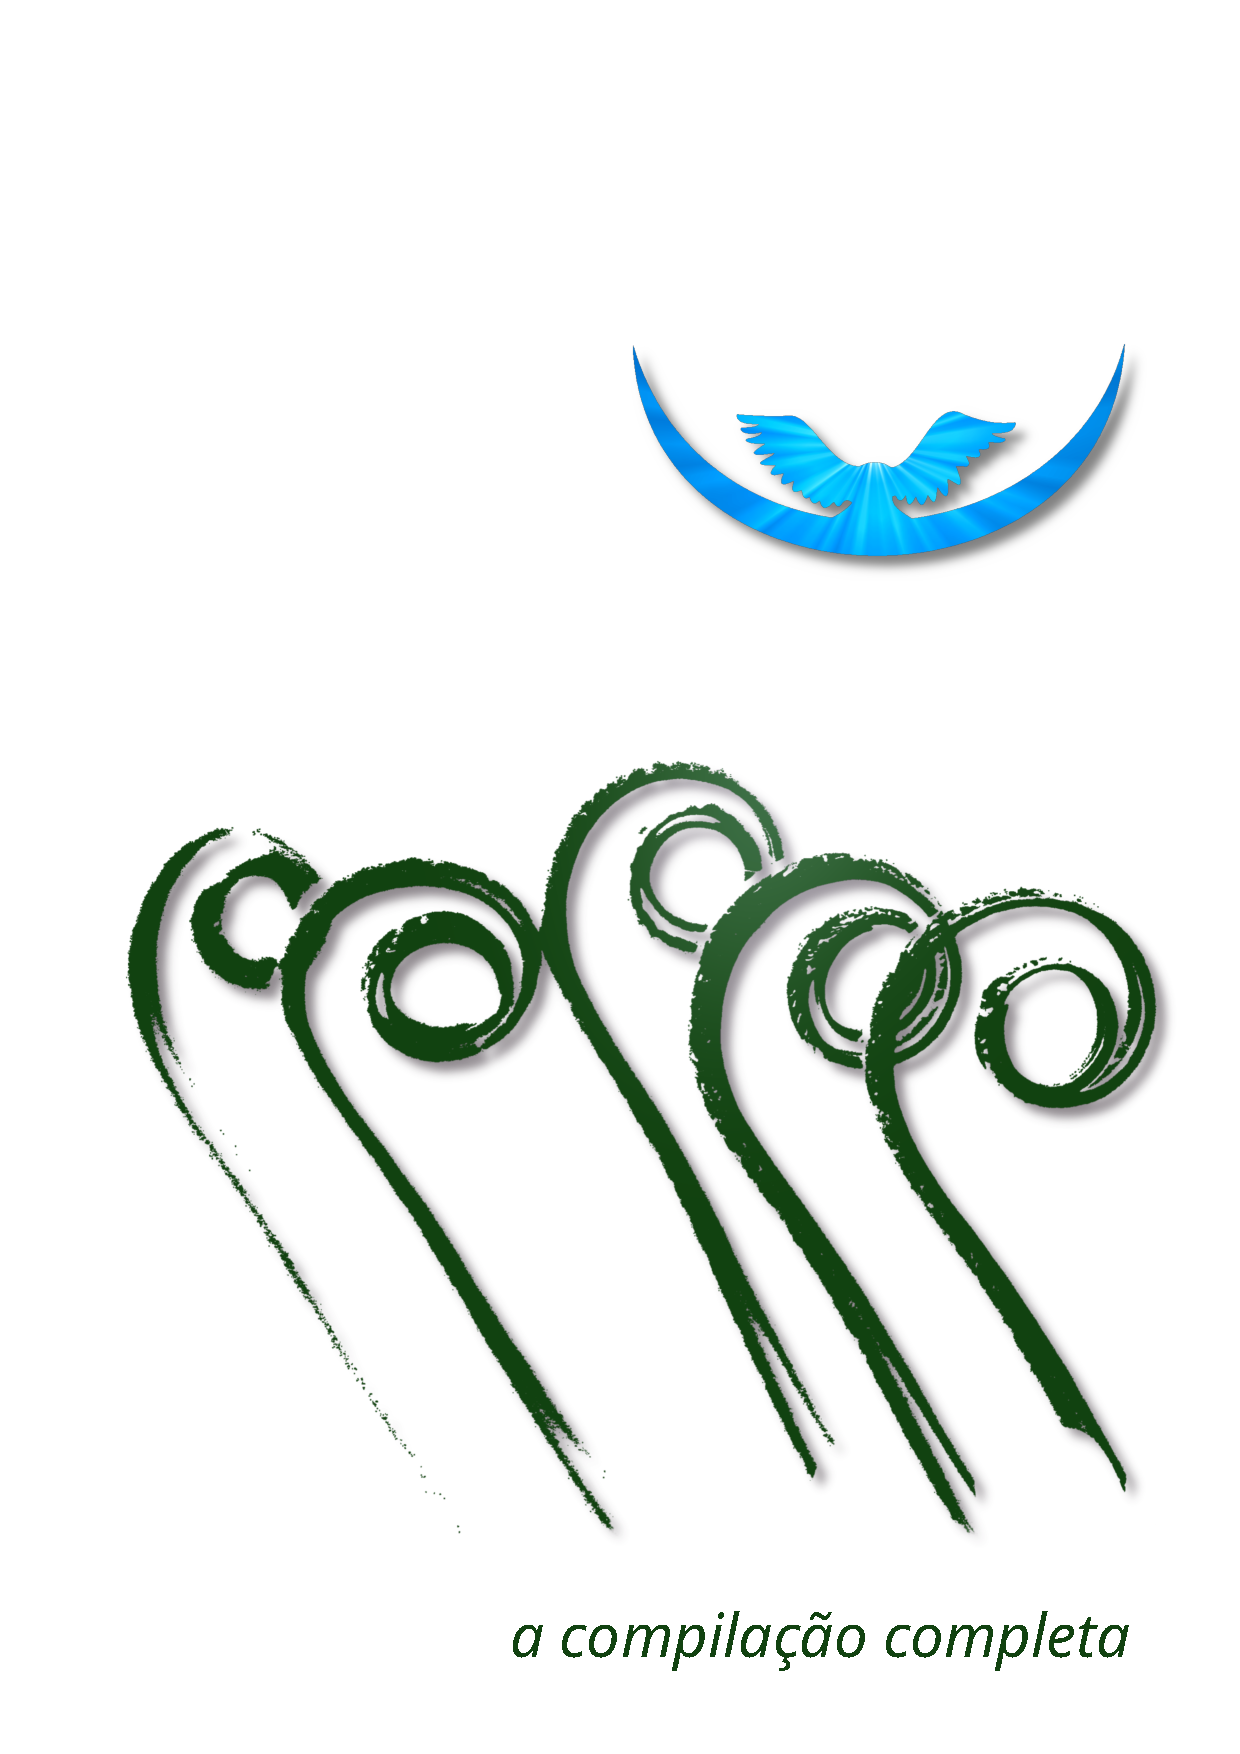
\includepdf[]{content/img/unilaiva-astral_COVER.pdf}
  % The second page (verso):
  \secondpage

  % TOC:
  \toc

  % Sets chapter number; will be incremented by one at each \mainchapter,
  % \songchapter or \chapter:
  \setcounter{chapter}{0}

  \mainchapter[]{Preces}
    \begin{songs}{}
      % Santo Daime: Preces
% ===================
%


{ % Put everything in this file in a block to not bleed settings

  % use Roman numerals for song (prayer) numbering:
  \renewcommand{\thesongnum}{\Roman{songnum}}
  % no chords here, so line spacing will be less:
  \chordsoff

  % Add a little more line spacing
  \baselineadj=+1pt plus 0pt minus 0pt

  % Use this to specify a subtitle -- used in Pai nosso + Ave Maria
  \newcommand{\subtitle}[1]{
    \vspace{2.618034ex}\textbf{\textit{#1}}\vspace{1.618034ex}
  }

  % Use this to specify a translation title within a verse, eg
  % \translationtitle{EN}{Greed}
  \newcommand{\translationtitle}[2]{
    \brkpenalty=-9000\brk%
    \vspace{2.618034ex}%
    \textbf{[#1]} \textit{#2}%
    \vspace{1.618034ex}%
  }
  % Use this to create a vertical space between "paragraphs"
  % within verses:
  \newcommand{\parspace}{\vspace{1ex}}

  % Setup the color for note mark superscripts to be the same as chords'
  % color:
  \definecolor{notemarkcolor}{rgb}{0,0,0}%
  \colorlet{notemarkcolor}{chordcolor}%

  % Redefine \up macro to use notemarkcolor
  \renewcommand{\up}[1]{
    \textsuperscript{\color{notemarkcolor}#1}%
  }

  % Environment for a multiline note to be used within a song environment:
  \newenvironment{note}{%
    \yesendsongvfill%
    \vfill%
    \beginverse*%
    \small%
    \begin{itshape}%
  }{%
    \end{itshape}%
    \endverse%
  }


  \scleardpage
  \songsection{Abertura}
  \setcounter{songnum}{1}

  \begin{songs}{}

    \beginsong{Sinal da Cruz}[tags={bailado, São Miguel, Mesa Branca}]
      \beginverse
        \up{1}Pelo sinal da Santa Cruz,
        \up{2}livrai-nos, Deus, nosso Senhor,
        \up{3}dos nossos inimigos
        \parspace
        \up{4}Em nome do Pai,
        \up{5}do Filho e
        \up{6}do Espírito \up{7}Santo.
        \parspace
        Amém.
      \endverse
      \beginverse\color{englishcolor}
        \translationtitle{EN}{Sign of the Cross}
        \up{1}By the sign of the Holy Cross,
        \up{2}deliver us, God, our Lord,
        \up{3}from our enemies
        \parspace
        \up{4}In the name of the Father,
        \up{5}the Son, and
        \up{6}the Holy \up{7}Spirit.
        \parspace
        Amen.
      \endverse
      \begin{note}
        While speaking the prayer, synchronously make
        the sign of the Cross with with your right thumb
        on your \up{1}forehead,
        on your \up{2}mouth, and
        on your \up{3}chest.
        \parspace
        Then, with your right hand, touch
        your \up{4}forehead,
        your \up{5}chest,
        your \up{6}left shoulder and \up{7}right shoulder.
      \end{note}
    \endsong


    \beginsong{Credo}[tags={bailado}]
      \baselineadj=0pt\relax% To fit
      \beginverse
        Creio em Deus Pai todo Poderoso,
        Criador do Céu e da terra.
        \parspace
        Creio em Jesus Cristo, um só seu filho, Nosso
        Senhor, o qual for concebido por obra e graça do
        Espírito Santo. Nasceu da Maria Virgem;
        padeceu sob o poder de Pôncio Pilatos;
        foi crucificado, morto e sepultado. Desceu aos
        infernos, ao terceiro dia ressurgiu dos mortos,
        Subiu ao Céu e Pai Todo-poderoso, de onde há de vir
        a julgar os vivos e os mortos.
        \parspace
        Creio no Espirito Santo, na Santa Igreja,
        na comunhão dos Santos, na remissão
        dos pecados, na ressurreição da carne,
        na vida eterna.
        \parspace
        Amém.
      \endverse
      \beginverse\color{englishcolor}
        \translationtitle{EN}{Creed}
        I believe in God, the Father Almighty,
        Creator of Heaven and earth.
        \parspace
        I believe in Jesus Christ, His only Son, Our Lord,
        who was conceived through the work and grace of
        the Holy Spirit. He was born of the Virgin Mary;
        suffered under the power of Pontius Pilate;
        was crucified, died, and was buried. He decended
        into Hell; on the third day he rose again from
        the dead. He ascended into Heaven and is seated
        at the right hand of God, the Father Almighty, from
        where He come to judge the living and the dead.
        \parspace
        I believe in the Holy Spirit, the Holy Church,
        the communion of Saints, the forgiveness of sins,
        the resurrection of the body, and life everlasting.
        \parspace
        Amen.
      \endverse
    %% Skip the Finnish version for now, to save space
    %   \beginverse\brk\vbox to0pt{}\vfill\color{finnishcolor}
    %     \translationtitle{FI}{Uskontunnustus}
    %     Minä uskon Jumalaan, Isään, Kaikkivaltiaaseen,
    %     taivaan ja maan Luojaan;
    %     \parspace
    %     ja Jeesukseen Kristukseen, Jumalan ainoaan Poikaan,
    %     meidän Herraamme, joka sikisi Pyhästä Hengestä,
    %     syntyi neitsyt Mariasta, kärsi Pontius Pilatuksen
    %     aikana, ristiinnaulittiin, kuoli ja haudattiin,
    %     astui alas tuonelaan, nousi kolmantena päivänä
    %     kuolleista, astui ylös taivaisiin, istuu Jumalan,
    %     Isän, Kaikkivaltiaan, oikealla puolella ja on sieltä
    %     tuleva tuomitsemaan eläviä ja kuolleita;
    %     \parspace
    %     ja Pyhään Henkeen, pyhän yhteisen seurakunnan,
    %     pyhäin yhteyden, syntien anteeksiantamisen,
    %     ruumiin ylösnousemisen ja iankaikkisen elämän.
    %     \parspace
    %     Aamen.
    %   \endverse
    \endsong


    \beginsong{Pai nosso \& Ave Maria}
      \beginverse
        \subtitle{Pai nosso}
        Pai nosso,
        que estais no Céu,
        santificado seja o Vosso Nome.
        Vamos nós ao Vosso Reino.
        Seja feita a Vossa Vontade,
        assim na terra como no Céu.
        O pão nosso de cada dia nos daí hoje, Senhor.
        Perdoai as nossas dividas,
        assim como nós perdoamos os nossos devedores.
        Não nos deixas, Senhor, cair em tentação,
        mas livrai-me e defendei-me, Senhor,
        de todo mal.
        \parspace
        Amém, Jesus, Maria, José.
      \endverse
      \beginverse
        \subtitle{Ave Maria}
        Ave Maria,
        cheia de Graça!
        O Senhor é convosco.
        Bendita sois Vós entre as mulheres.
        Bendito é o fruto do Vosso ventre, Jesus.
        Santa Maria, Mãe de Deus,
        rogai a Deus por nos pecadores,
        agora e na hora de nossa morte.
        \parspace
        Amém, Jesus, Maria, José.
      \endverse
      \forcebrk\vspace*{\fill}
      \beginverse\color{englishcolor}
        \translationtitle{EN}{Our Father}
        Our Father,
        who art in Heaven,
        hallowed be Thy Name.
        Let us go into Thy Kingdom.
        Thy Will be done,
        on earth as it is in Heaven.
        Give us this day our daily bread, Lord.
        Forgive us our debts,
        as we forgive our debtors.
        Let us not fall in temptation,
        but deliver me and defend me, Lord,
        from all evil.
        \parspace
        Amen, Jesus, Mary, Joseph.
      \endverse
      \beginverse\color{englishcolor}
        \translationtitle{EN}{Hail Mary}
        Hail Mary,
        full of grace!
        The Lord is with Thee.
        Blessed art Thou amongst women!
        Blessed is the fruit of Thy womb, Jesus.
        Holy Mary, Mother of God,
        pray to God for us sinners,
        now and at the hour of our death.
        \parspace
        Amen, Jesus, Mary, Joseph.
      \endverse
      \vspace*{\fill}
    \endsong


    \beginsong{O Terço I (trabalho officiais)}[tags={bailado}]
      \beginverse
        \textnotefornext{Ao rezar o terço, só diz a cada dezena:}
        \parspace
        Gloria ao Pai, ao Filho, ao Espírito Santo.
        Assim como era no princípio, agora e sempre,
        por todos os séculos dos séculos.
        \parspace
        Amém.
      \endverse
      \beginverse\color{englishcolor}
        \translationtitle{EN}{The Rosary I (official work)}
        \textnotefornext{While praying the Rosary, after every decade:}
        \parspace
        Glory to the Father, to the Son and to the Holy Spirit.
        As it was in the beginning, is now, and ever shall be,
        for all the ages of the ages.
        \parspace
        Amen.
      \endverse
    \endsong


    \begin{intersong}
      \textnotefornext{Ao fim do terço, (normalmente) a comandante do pelotão feminino:}
      \parspace
      Em nome de Deus Pai Todo-Poderoso, da Virgem Soberana Mãe,\\
      do Nosso Senhor Jesus Cristo, do Patriarca São José e de\\
      todos os Seres Divinos da Corte Celestial, com a ordem de\\
      nosso Mestre Império Juramidam, estão abertos os nossos\\
      trabalhos, meus irmãos e minhas irmãs. Que Deus e a Virgem Mãe\\
      sejam nossos guias para sempre. Amém!\\
      \emph{(Todos se benzem.)}\\
      \parspace\color{englishcolor}
      \textnotefornext{\textbf{[EN]} At the end of Rosary, (usually) the commander of the feminine batallion:}
      \parspace
      In the name of God the Almighty Father, of the Sovereign Virgin
      Mother, of Our Lord Jesus Christ, of the Patriarch Saint Joseph and of\\
      all the Divine Beings of the Celestial Court, with the order of our Master
      Governor Juramidam, our works are open, my brothers and sisters.\\
      May God and the Virgin Mother be our guides forever. Amen!\\
      \emph{(All make the sign of the cross.)}\\
    \end{intersong}


    \beginsong{O Terço II (Santa Missa)}[tags={Santa Missa}]
      \beginverse
        \textnotefornext{Ao rezar o terço, só diz a cada dezena:}
        \parspace
        Gloria ao Pai, ao Filho, ao Espírito Santo.
        Assim como era no princípio, agora e sempre,
        por todos os séculos dos séculos.
        \parspace
        Amém.
        \parspace\parspace
        Oh! meu Jesus, perdoai-me, livrai-me do fogo do
        inferno. Levai as almas todas para o Céu, e soccorei
        principalmente aquelas que mais precísarem.
        \parspace
        Amém.
      \endverse
      \beginverse\color{englishcolor}
        \translationtitle{EN}{The Rosary II (Santa Missa)}
        \textnotefornext{While praying the Rosary, after every decade:}
        \parspace
        Glory to the Father, to the Son and to the Holy Spirit.
        As it was in the beginning, is now, and ever shall be,
        for all the ages of the ages.
        \parspace
        Amen.
        \parspace\parspace
        Oh my Jesus, forgive me, and save me from the fires
        of hell. Lead all souls into heaven, and especially
        help those in most need.
        \parspace
        Amen.
      \endverse
    \endsong


    \beginsong{Chave de Harmonia}[tags={trabalhos de mesa}]
      \beginverse
        Desejo Harmonia, Amor, Verdade e Justiça a todos os
        meus irmãos.
        \ind Com as forças reunidas das silenciosas vibrações
        dos nossos pensamentos, somos fortes, sádios e
        felizes, formando assim um elo de fraternidade
        universal.
        \ind Estou satisfeito e em paz com o universo inteiro
        e desejo que todos os seres realizam as suas
        aspirações mais íntímas.
        \ind Dou graças ao Pai Invisivel por ter estabelecido
        a Harmonia, o Amor, a Verdade e a Justiça entre
        todos os seus filhos.
        \parspace
        Assim seja, Amém.
      \endverse
      \beginverse\color{englishcolor}
        \translationtitle{EN}{Key of Harmony}
        I wish Harmony, Love, Truth and Justice to all my
        brothers and sisters.
        \ind With the united forces of the silent vibrations
        of our thoughts, we are strong, healthy and happy,
        thus forming a link of universal fraternity.
        \ind I am satisfied and in peace with the whole
        universe, and I wish that all beings achieve their
        most intimate aspirations.
        \ind I give thanks to my Invisible Father for having
        established Harmony, Love, Truth and Justice among
        all his children.
        \parspace
        So be it, Amen.
      \endverse
    \endsong


    \sclearpage
    \beginsong{Consagração do Aposento}
      \textnotefornext{Nos trabalhos de mesa: após Hinos da Oração}
      \parspace
      \beginverse
        Dentro do Circulo Infinito da Divina Presença que
        me envolve inteiramente, afirmo:
        \parspace
        Há uma só presença aqui --- é a da HARMONIA que faz
        vibrar todos os corações de felicidade e alegria.
        Quem quer que aqui entre, sentirá as vibrações da
        Divina Harmonia.
        \parspace
        Há uma só presença aqui --- é a do AMOR. Deus é o
        Amor que envolve todos os seres num só sentimento
        de unidade. Este recinto está cheio da presença do
        Amor. No Amor eu vivo, me movo e existo. Quem quer
        que aqui entre, sentirá a pura e Santa Presença do
        Amor.
        \parspace
        Há uma só presença aqui --- é a da VERDADE. Tudo
        que aqui existe, tudo o que aqui se fala, tudo o
        que aqui se pensa é a expressão da Verdade. Quem
        quer que aqui entre, sentirá a Presença da Verdade.
        \parspace
        Há uma só presença aqui --- é a da JUSTIÇA.
        A Justiça reina neste recinto. Todos os atos aqui
        praticados são regidos e inspirados pela Justiça.
        Quem quer que aqui entre, sentirá
        a Presença da Justiça.
        \parspace
        Há uma só presença aqui --- é a presença de Deus,
        o BEM. Nenhum mal pode entrar aqui. Não há mal em
        Deus. Deus, o Bem, reside aqui. Quem quer que aqui
        entre, sentirá a Presença Divina do Bem.
        \parspace
        Há uma só presença aqui --- é a presença de Deus,
        a VIDA. Deus é a Vida essencial de todos os seres.
        É a saúde do corpo e da mente. Quem quer que aqui
        entre, sentirá a Divina Presença da Vida e da Saúde.
        \parspace
        Há uma só presença aqui --- é a presença de Deus,
        a PROSPERIDADE. Deus é Prosperidade, pois Ele faz
        tudo crescer e prosperar. Deus se expressa na
        Prosperidade de tudo o que aqui é empreendido em
        seu nome. Quem quer que aqui entre, sentirá
        a Divina Presença da Prosperidade e da Abundância.
        \parspace
        Pelo símbolo esotérico das Asas Divinas, estou
        em vibração harmoniosa com as Correntes Universais
        da Sabedoria, do Poder e da Alegria. A Presença
        da Divina Sabedoria manifesta-se aqui. A presença
        da Alegria Divina é profundamente sentida por todos
        os que aqui entram.
        \parspace
        Na mais perfeita comunhão entre o meu eu inferior
        e o meu Eu Superior, que é Deus em mim, consagro
        este recinto à perfeita expressão de todas as
        qualidades Divinas que há em mim, e em todos os
        seres.
        \parspace
        As vibrações do meu pensamento são forças de Deus
        em mim, que aqui ficam armazenadas e daqui se
        irradiam para todos os seres, constituindo este
        lugar um centro de emissão e recepção de tudo
        quanto é BOM, ALEGRE, e PRÓSPERO.
        \parspace
        \textbf{ORAÇÃO}
        \parspace
        Agradeço-Te o Deus, porque este recinto está cheio
        da Tua Presença.
        \parspace
        Agradeço-Te, porque vivo e me movo por Ti.
        \parspace
        Agradeço-Te, porque vivo em tua Vida, Verdade e
        Saúde, Prosperidade, Paz, Sabedoria, Alegria e Amor.
        \parspace
        Agradeço-Te, porque todos que entrarem aqui sentirão
        Tua Presença.
        \parspace
        Agradeço-Te, porque estou em Harmonia, Amor, Verdade
        e Justiça com todos os seres.
        \parspace
        Amém.
      \endverse
      \beginverse\color{englishcolor}
        \translationtitle{EN}{Consecration of the Space}
        \textnotefornext{In sitting works: after Oração}
        \parspace
        Inside the Infinite Circle of the Divine Presence
        which completely surrounds me, I affirm that:
        \parspace
        There is only one presence here --- it is HARMONY,
        which makes all hearts vibrate with joy and happiness.
        Those who choose to enter here will feel the vibration
        of Divine Harmony.
        \parspace
        There is only one presence here --- it is LOVE.
        God is love, which embraces all beings in one
        feeling of unity. This space is filled with the
        presence of Love. In Love, I live, I move and I
        exist. Those who choose to enter here will feel
        the pure and holy Presence of Love.
        \parspace
        There is only one presence here --- it is TRUTH.
        All that exists here, all that is spoken here,
        all that is thought here is the expression of
        Truth. Those who choose to enter here will feel
        the Presence of Truth.
        \parspace
        There is only one presence here --- it is JUSTICE.
        Justice reigns in this space. Everything practiced
        here is inspired and ruled by Justice. Those who
        choose to enter here will feel the Presence of
        Justice.
        \parspace
        There is only one presence here --- it is the
        presence of God, the BENEFICIENT. No evil can enter
        here. There is no evil in God. God, the Beneficient,
        dwells here. Those who choose to enter here will
        feel the Divine Presence of the Beneficient.
        \parspace
        There is only one presence here --- it is the
        presence of God, who is LIFE. God is the essential
        Life of all beings, the health of body and mind.
        Those who choose to enter here will feel the Divine
        Presence of Life and Health.
        \parspace
        There is only one presence here --- it is the
        presence of God, who is PROSPERITY. God is
        Prosperity because He makes everything grow and
        prosper. God expresses Himself through the
        Prosperity of all that is undertaken in His name.
        Those who choose to enter here will feel the
        Divine Presence of Prosperity and Abundance.
        \parspace
        Through the esoteric symbol of the Divine Wings,
        I am in harmonious vibration with the universal
        currents of Wisdom, Power and Joy. The Presence
        of Divine Wisdom is manifested here. The Presence
        of Divine Joy is deeply felt by all those who choose
        to enter here.
        \parspace
        In the perfect communion between my lower self and
        my Higher Self, which is God in me, I consecrate
        this space to the perfect expression of all Divine
        qualities which are in me and in all beings.
        \parspace
        The vibrations of my thoughts are the forces of God
        in me, which are stored here and hence radiate to
        all beings, thus establishing this place as a center
        of giving and receiving of all that is GOOD, JOYFUL
        and PROSPEROUS.
        \parspace
        \textbf{PRAYER}
        \parspace
        I thank You, oh God, for this space is filled with
        Your Presence.
        \parspace
        I thank you, for I live and move within You.
        \parspace
        I thank You, for I live in Your Life, Truth, Health,
        Prosperity, Peace, Wisdom, Joy and Love.
        \parspace
        I thank You, for all those who enter here will feel
        Your Presence.
        \parspace
        I thank You, for I am in Harmony, Love, Truth and
        Justice with all beings.
        \parspace
        Amen.
      \endverse
      \beginverse\color{finnishcolor}
        \translationtitle{FI}{Paikan pyhittäminen}
        \textnotefornext{Istumatöissä: Oraçãon jälkeen}
        \parspace
        Jumalallisen läsnäolon äärettömästä piiristä käsin,
        joka ympäröi minut täysin, todistan:
        \parspace
        Täällä on vain yksi läsnäolo, HARMONIAN läsnäolo,
        joka saa kaikkien sydämet värähtelemään  onnea ja
        iloa. Kuka tahansa, joka tulee tähän tilaan, saa
        tuntea jumalallisen harmonian värähtelyn.
        \parspace
        Täällä on vain yksi läsnäolo, RAKKAUDEN läsnäolo.
        Jumala on rakkaus, joka syleilee kaikkia olentoja
        kaikenkattavalla ykseyden tunteella. Tämä paikka on
        täynnä rakkauden läsnäoloa. Rakkaudessa minä elän,
        liikun ja olen. Kuka tahansa, joka tulee tähän tilaan,
        saa tuntea rakkauden puhtaan ja pyhän läsnäolon.
        \parspace
        Täällä on vain yksi läsnäolo, TOTUUS. Kaikki mitä
        täällä on, kaikki mitä täällä puhutaan, kaikki mitä
        täällä ajatellaan on totuuden ilmaisua. Kuka tahansa,
        joka tulee tähän tilaan, saa tuntea totuuden läsnäolon.
        \parspace
        Täällä on vain yksi läsnäolo, OIKEUS. Oikeus hallitsee
        tässä paikassa. Kaikki täällä tehdyt teot ovat oikeuden
        johtamia ja inspiroimia. Kuka tahansa, joka tulee tähän
        tilaan, saa tuntea oikeuden läsnäolon.
        \parspace
        Täällä on vain yksi läsnäolo, Jumalan läsnäolo, HYVYYS.
        Mikään paha ei pääse tänne. Jumalassa ei ole pahaa.
        Jumala, joka on hyvyys, asuu täällä. Kuka tahansa, joka
        tulee tähän tilaan, saa tuntea hyvyyden jumalallisen
        läsnäolon.
        \parspace
        Täällä on vain yksi läsnäolo, Jumalan läsnäolo, joka on
        ELÄMÄ. Jumala on kaikkien olentojen elämän ydin.
        Mielen ja ruumiin terveys. Kuka tahansa, joka tulee
        tähän tilaan, saa tuntea elämän ja terveyden jumalallisen
        läsnäolon.
        \parspace
        Täällä on vain yksi läsnäolo, KUKOISTUS. Jumala on kukois-
        tus, koska Hän saa kaiken kasvamaan ja menestymään.
        Jumala ilmaisee itseään kaiken sen kukoistamisessa,
        mihin täällä ryhdytään Hänen nimessään. Kuka tahansa,
        joka tulee tähän tilaan, tuntee kukoistamisen ja
        yltäkylläisyyden jumalallisen läsnäolon.
        \parspace
        Jumalallisten siipien esoteerisen symbolin kautta
        värähtelen harmoniassa VIISAUDEN, VOIMAN ja ILON
        universaalien virtausten kanssa. Jumalallisen viisauden
        läsnäolo ilmentyköön täällä. Jumalallisen ilon
        läsnäolon tuntevat syvästi kaikki ne, jotka tähän
        tilaan saapuvat.
        \parspace
        Mitä täydellisimmässä yhteydessä alemman minäni ja
        korkeamman minäni välillä, joka on Jumala minussa,
        pyhitän tämän paikan kaikkien niiden jumalallisten
        ominaisuuksien täydelliselle ilmaisulle, jotka ovat
        minussa ja kaikissa olennoissa.
        \parspace
        AJATUSTENI värähtelyt ovat Jumalan voimia minussa,
        jotka kootaan täällä ja lähetetään täältä kaikille
        olennoille, niin että tästä paikasta tulee keskus,
        josta lähetetään ja vastaanotetaan kaikkea, mikä on
        HYVÄÄ, ILOISTA ja KUKOISTAVAA.
        \parspace
        \textbf{RUKOUS}
        \parspace
        Kiitän sinua, oi Jumala, koska tämä paikka on täynnä
        sinun läsnäoloasi.
        \parspace
        Kiitän sinua, koska elän ja liikun sinussa.
        \parspace
        Kiitän sinua, koska elän sinun Elämässäsi, Totuudessasi,
        Terveydessäsi, Kukoistuksessasi, Rauhassasi,
        Viisaudessasi, Ilossasi ja Rakkaudessasi.
        \parspace
        Kiitän sinua, koska kaikki jotka saapuvat tänne saavat
        tuntea sinun läsnäolosi.
        \parspace
        Kiitän sinua, koska olen Harmoniassa, Rakkaudessa,
        Totuudessa ja Oikeudessa kaikkien olentojen kanssa.
        \parspace
        Aamen.
      \endverse
    \endsong


    \begin{intersong}
      % to sit between starting and ending prayers
      \imagecc[4]{SD_cross_simple_flat_blueish_transparent_bg.png}
    \end{intersong}


  \end{songs}



  \scleardpage
  \songsection{Encerramento}
  \setcounter{songnum}{1}

  \begin{songs}{}


    \beginsong{Pai nosso \& Ave Maria}
      \beginverse
        \subtitle{Pai nosso}
        Pai nosso,
        que estais no Céu,
        santificado seja o Vosso Nome.
        Vamos nós ao Vosso Reino.
        Seja feita a Vossa Vontade,
        assim na terra como no Céu.
        O pão nosso de cada dia nos daí hoje, Senhor.
        Perdoai as nossas dividas,
        assim como nós perdoamos os nossos devedores.
        Não nos deixas, Senhor, cair em tentação,
        mas livrai-me e defendei-me, Senhor,
        de todo mal.
        \parspace
        Amém, Jesus, Maria, José.
      \endverse
      \beginverse
        \subtitle{Ave Maria}
        Ave Maria,
        cheia de Graça!
        O Senhor é convosco.
        Bendita sois Vós entre as mulheres.
        Bendito é o fruto do Vosso ventre, Jesus.
        Santa Maria, Mãe de Deus,
        rogai a Deus por nos pecadores,
        agora e na hora de nossa morte.
        \parspace
        Amém, Jesus, Maria, José.
      \endverse
      \forcebrk\vspace*{\fill}
      \beginverse\color{englishcolor}
        \translationtitle{EN}{Our Father}
        Our Father,
        who art in Heaven,
        hallowed be Thy Name.
        Let us go into Thy Kingdom.
        Thy Will be done,
        on earth as it is in Heaven.
        Give us this day our daily bread, Lord.
        Forgive us our debts,
        as we forgive our debtors.
        Let us not fall in temptation,
        but deliver me and defend me, Lord,
        from all evil.
        \parspace
        Amen, Jesus, Mary, Joseph.
      \endverse
      \beginverse\color{englishcolor}
        \translationtitle{EN}{Hail Mary}
        Hail Mary,
        full of grace!
        The Lord is with Thee.
        Blessed art Thou amongst women!
        Blessed is the fruit of Thy womb, Jesus.
        Holy Mary, Mother of God,
        pray to God for us sinners,
        now and at the hour of our death.
        \parspace
        Amen, Jesus, Mary, Joseph.
      \endverse
      \vspace*{\fill}
    \endsong


    \beginsong{Credo}[tags={Mesa Branca, São Miguel}]
      \baselineadj=0pt\relax% To fit
      \beginverse
        Creio em Deus Pai todo Poderoso,
        Criador do Céu e da terra.
        \parspace
        Creio em Jesus Cristo, um só seu filho, Nosso
        Senhor, o qual for concebido por obra e graça do
        Espírito Santo. Nasceu da Maria Virgem;
        padeceu sob o poder de Pôncio Pilatos;
        foi crucificado, morto e sepultado. Desceu aos
        infernos, ao terceiro dia ressurgiu dos mortos,
        Subiu ao Céu e Pai Todo-poderoso, de onde há de vir
        a julgar os vivos e os mortos.
        \parspace
        Creio no Espirito Santo, na Santa Igreja,
        na comunhão dos Santos, na remissão
        dos pecados, na ressurreição da carne,
        na vida eterna.
        \parspace
        Amém.
      \endverse
      \beginverse\color{englishcolor}
        \translationtitle{EN}{Creed}
        I believe in God, the Father Almighty,
        Creator of Heaven and earth.
        \parspace
        I believe in Jesus Christ, His only Son, Our Lord,
        who was conceived through the work and grace of
        the Holy Spirit. He was born of the Virgin Mary;
        suffered under the power of Pontius Pilate;
        was crucified, died, and was buried. He decended
        into Hell; on the third day he rose again from
        the dead. He ascended into Heaven and is seated
        at the right hand of God, the Father Almighty, from
        where He come to judge the living and the dead.
        \parspace
        I believe in the Holy Spirit, the Holy Church,
        the communion of Saints, the forgiveness of sins,
        the resurrection of the body, and life everlasting.
        \parspace
        Amen.
      \endverse
      % Keep the Finnish version here, as we need something for the recto page :)
      \beginverse\brk\vbox to0pt{}\vfill\color{finnishcolor}
        \translationtitle{FI}{Uskontunnustus}
        Minä uskon Jumalaan, Isään, Kaikkivaltiaaseen,
        taivaan ja maan Luojaan;
        \parspace
        ja Jeesukseen Kristukseen, Jumalan ainoaan Poikaan,
        meidän Herraamme, joka sikisi Pyhästä Hengestä,
        syntyi neitsyt Mariasta, kärsi Pontius Pilatuksen
        aikana, ristiinnaulittiin, kuoli ja haudattiin,
        astui alas tuonelaan, nousi kolmantena päivänä
        kuolleista, astui ylös taivaisiin, istuu Jumalan,
        Isän, Kaikkivaltiaan, oikealla puolella ja on sieltä
        tuleva tuomitsemaan eläviä ja kuolleita;
        \parspace
        ja Pyhään Henkeen, pyhän yhteisen seurakunnan,
        pyhäin yhteyden, syntien anteeksiantamisen,
        ruumiin ylösnousemisen ja iankaikkisen elämän.
        \parspace
        Aamen.
      \endverse
    \endsong


    \sclearpage
    \beginsong{Prece de Cáritas}[tags={cura}]
      \beginverse
        Deus, nosso Pai que sois todo Poder e Bondade, dai
        a força àquele que passa pela provação.
        \ind Dai a luz àquela que procura a verdade.
        \ind Ponde no coração do homem a compaixão e a caridade.
        \ind Deus! Dai ao viajor a estrela guia; ao aflito,
        a consolação; ao doente, o repouso!
        \ind Pai, dai ao culpado, o arrependimento; ao espírito,
        a verdade; à criança, o guia; ao órfão, o pai!
        \ind Senhor, que a Vossa bondade se estenda sobre tudo
        que criastes.
        \ind Piedade, Senhor, para aqueles que Vos não conhecem.
        \ind Esperança para aqueles que sofrem.
        \ind Que a Vossa bondade permita aos espíritos
        consoladores derramarem por toda a parte a paz, a
        esperança e a fé.
        \ind Deus! Um raio, uma faísca do Vosso amor pode abraçar
        a terra.
        \ind Deixa-nos beber na fonte dessa bondade fecunda
        e infinita e todas as lágrimas secarão e todas as
        dores se acalmarão.
        \ind Um só coração, um só pensamento subirá até Vós,
        como um grito de reconhecimento e de Amor.
        \ind Como Moisés sobre as montanha nós Vós esperamos
        com os braços abertos.
        \ind O Poder, o Bondade, o Beleza, o Perfeição, e
        queremos de alguma sorte merecer a Vossa infinita
        misericórdia.
        \ind Deus, dai-nos a força de ajudar o progresso a fim
        de subir-nos até Vós.
        \ind Dai-nos a caridade pura, dai-nos a fé e a razão.
        \ind Dai-nos a simplicidade que fará de nossas almas o
        espelho aonde se deve refletir a Vossa imagem.
        \parspace
        Amém.
      \endverse
      \forcebrk
      \vspace*{-1.1em}
      \beginverse\color{englishcolor}
        \translationtitle{EN}{Prayer of Caritas}
        God, our Father who is all Power and Kindness,
        give strength to those who're going through
        their trials.
        \ind Give light to those who are seeking the truth.
        \ind Put in the hearts of men compassion and charity.
        \ind God, give to the one who travels, a guiding star;
        to the afflicted, consolation; to the sick, rest.
        \ind Father, give to the guilty, repentance; to the
        spirit, truth; to the child, a guide; to the orphan,
        a father.
        \ind Lord, may Your kindness spread above all that You
        have created.
        \ind Mercy, Lord, for those who don't know You.
        \ind Hope for those who suffer.
        \ind May Your kindness allow the consoling spirits to
        spread everywhere Peace, Hope and Faith.
        \ind God, one ray, one spark of Your Love can enlighten
        the earth.
        \ind Let us drink in the fountain of this fertile and
        infinite kindness, and all tears will dry, and all pains
        will quiet down.
        \ind One single heart, one single thought will go up to
        You, like a cry of thankfullness and of love.
        \ind Like Moses on the mountain, we await for You with
        open arms.
        \ind Oh Power, oh Kindness, oh Beauty, oh Perfection,
        we want, in some way, to deserve Your infinite Mercy!
        \ind God, give us the strength to support the progress,
        in order to rise up to You.
        \ind Give us pure Charity, give us Faith and Reason.
        \ind Give us the simplicity that will make our souls the
        mirror where Your image must be reflected.
        \parspace
        Amen.
      \endverse
    \endsong


    \beginsong{Salve Rainha}
      \beginverse
        Deus Vós salve, oh! Rainha, Mãe de Misericórdia,
        vida, doçura, esperança nossa, salve!
        \ind A Vós bradamos, os degredados filhos de Eva.
        \ind A Vós suspiramos, gemendo, e chorando neste
        vale de lágrimas.
        \ind Eia pois, advogada nossa, esses Vossos olhos
        misericordiosos a nós volveis.
        \ind E depois deste desterro mostrai-nos Jesus.
        \ind Bendito é o fruto do Vosso Ventre!
        \ind Oh! Clemente, oh! Piedosa, oh! Doce, sempre
        Virgem Maria!
        \ind Rogai a Deus por nós, Santíssima Mãe de Deus,
        para que sejamos dignos de alcançar as promessas
        de nosso Senhor Jesus Cristo, Senhor nosso.
        \parspace
        Amém, Jesus, Maria, e José.
      \endverse
      \beginverse\color{englishcolor}
        \translationtitle{EN}{Hail Holy Queen}
        Hail Holy Queen, Mother of Mercy, our life, our
        sweetness and our hope.
        \ind To You do we cry, poor banished children of Eve;
        \ind to You do we send up our sighs, mourning and
        weeping in this valley of tears.
        \ind Turn then, O most Gracious Advocate, Your eyes
        of mercy towards us.
        \ind And after this, our exile, show unto us the
        blessed fruit of your womb, Jesus.
        \ind O! Clement, o! loving, o! sweet Virgin Mary!
        \ind Pray for us o Holy Mother of God, that we may
        be worthy of the promises of our Lord Jesus Christ,
        our Lord forever.
        \parspace
        Amen, Jesus, Mary and Joseph.
      \endverse
    \endsong


    \beginsong{Encerramento}
      \beginverse
        \textnotefornext{Dirigente do trabalho pronuncia:}
        Em nome de Deus Pai Todo-Poderoso, da Virgem
        Soberana Mãe, do Patriarca São José e de todos
        os Seres Divinos da Corte Celestial, e com
        a Ordem do nosso Mestre Império Juramidam,
        está encerrado o nosso trabalho, meus irmãos
        e minhas irmãs.
        \textbf{Louvado seja Deus nas alturas!}
        \parspace
        \textnotefornext{E todos respondem:}
        Para que sempre seja louvada a nossa Mãe Maria
        Santíssima, sobre toda a humanidade. Amém!
      \endverse
      \beginverse\color{englishcolor}
        \translationtitle{EN}{Closing}
        \textnotefornext{Leader of the work pronounces:}
        In the name of God the Almighty Father, of the Sovereign
        Virgin Mother, of the Patriarch Saint Joseph and of all
        the Divine Beings of the Celestial Court, and with
        the Order of our Master Governor Juramidam,
        our work is ended, my brothers and my sisters.
        \textbf{Praised be God in the Heights!}
        \parspace
        \textnotefornext{And all respond:}
        May our Mother, the Most Holy Mary, be forever
        praised above all humanity. Amen!
      \endverse
    \endsong


    \beginsong{Sinal da Cruz}
      \beginverse
        \up{1}Pelo sinal da Santa Cruz,
        \up{2}livrai-nos, Deus, nosso Senhor,
        \up{3}dos nossos inimigos
        \parspace
        \up{4}Em nome do Pai,
        \up{5}do Filho e
        \up{6}do Espírito \up{7}Santo.
        \parspace
        Amém.
      \endverse
      \beginverse\color{englishcolor}
        \translationtitle{EN}{Sign of the Cross}
        \up{1}By the sign of the Holy Cross,
        \up{2}deliver us, God, our Lord,
        \up{3}from our enemies
        \parspace
        \up{4}In the name of the Father,
        \up{5}the Son, and
        \up{6}the Holy \up{7}Spirit.
        \parspace
        Amen.
      \endverse
      \begin{note}
        While speaking the prayer, synchronously make
        the sign of the Cross with with your right thumb
        on your \up{1}forehead,
        on your \up{2}mouth, and
        on your \up{3}chest.
        \parspace
        Then, with your right hand, touch
        your \up{4}forehead,
        your \up{5}chest,
        your \up{6}left shoulder and \up{7}right shoulder.
      \end{note}
    \endsong

  \end{songs}

}

    \end{songs}

  \mainchapter[]{Oração \chapsymbol{lightgray}}
    \begin{songs}{}
      % Santo Daime: Oração
% ===================
%
\audio[title={Nossa Irmandade}]{https://www.nossairmandade.com/hinario/1/Ora\%C3\%A7\%C3\%A3o}
\audio[title={Ceu da Santa Luz}]{https://www.youtube.com/watch?v=wKMY4YGdYeY}

% The following sets the song number for the first song in this file.
% The number will automatically be incremented by one for each song.
% Please do not change this! Changing would make different versions of
% the songbook to have different numbers for the same songs, and it
% would totally mess up the selection booklets causing them to have
% wrong songs in them. (For the same reason, add new songs only to the
% end of each songs_ file.)
\setcounter{songnum}{1}


\beginsong{Examine a Consciência}[by={Padr. Sebastião}, key={C}, sks={D, C--E}]
  \audio[]{https://www.nossairmandade.com/hymn/1/ExamineAConsci\%C3\%AAncia}
  \audio[key={C},title={Ceu da Santa Luz}]{https://www.youtube.com/watch?v=wKMY4YGdYeY\&t=18s}
  \mnbeginchorus\memorize
    \[^\mn{G}]E\[^\mn{C}]xa|\[\mnc{E}C]mine a \[\bmc\mn{D}]con\[^\mn{C}]sci|\[\mnc{G}G]ência \altchords{\id[1]{(D)}|D |A}
    \[\bm]E\[^\mn{C}]xa|\[\mnc{E}Am]mine \[\bmc\mn{D}]di\[^\mn{C}]rei|\[\mnc{G}G]ti\[\bm]nho \altchords{|Bm |A}
    \[^\mn{C}]Sou |\[\mnc{E}C]Pai e \[\bmc\mn{D}]não \[^\mn{C}]sou |\[\mnc{G}G]filho \altchords{|D |A}
    \[\bm]Mas \[^\mn{C}]eu |\[\mnc{E}Am]não fa\[\mnc{D}G]ço \[^\mn{E}]as|\[\mnc{C}C]sim\[\bm] \altchords{|Bm A |D}
  \mnendchorus
  \notesoff
  \beginchorus
    Cha|^mo de ^um a |^um
    A ^todos |^eu mos^tro o ca|^mi^nho
    Fa|^zendo ^como eu |^mando
    ^Tudo |^fica ^bem fa|^ci^nho
  \endchorus
  \beginchorus
    Todos |^podem ^se lem|^brar^ \altchords{\id[3]{MK (C)} |C G7 |C}
    Do |^tempo ^de No|^é ^ \altchords{|Am Dm7 |G}
    \noteson \[\mnlow{G}]A \[\mnlow{C}]dou\notesoff|^trina ^do meu |^Pai \altchords{|C G7 |C}
    ^Eu en|^sino ^como |^é ^ \altchords{|Am G7 |C}
  \endchorus
  \beginchorus
    |^Vamos ^meus ir|^mãos
    ^Vamos |^todos se ^humi|^lhar^
    Pe|^dir nos^so per|^dão
    Para ^nosso |^Pai nos ^perdo|^ar ^
  \endchorus
  \beginchorus
    Quem qui|^ser que se ^agu|^ente \altchords{\id[5]{simple (C)} |C G |C}
    ^Não tem |^{a quem} ^se quei|^xar^ \altchords{| - G |C}
    Eu |^bem que ^avi|^sei \altchords{| - G |C}
    ^Que ha|^via ^de che|^gar^ \altchords{| - G |C}
  \endchorus
  \begin{lilywrap}\begin{lilypond}[] \include "tex/lp-include-head.ly"
    theMelody = \relative c'' {
      \set melismaBusyProperties = #'() \slurDashed
      \key c \major \time 4/4 \partial 4
      \repeat volta 2 {
        g8( \pomark << \parenthesize g) c >> | e4 e8( e8) d4 c4 | g4.( g8)( g4) c
        | e4 e8( e8) d4 c | g'2( g4) \once\slurUp << \parenthesize g,8( c >> c8)
        | e4. e8 d4 c | g4( g8)( g8) g4 c
        | e4 e d e | c2( c4)
      }
    }
    theLyricsOne = \lyricmode {
      \set stanza = "1."
      \repeat volta 2 {
        E -- xa -- | mi -- ne a con -- ci -- | ên -- cia;
        E -- xa -- | mi -- ne __ _ di -- rei -- | ti -- nho;
        Sou __ _ | Pai e não sou | fil -- _ ho;
        Mas eu | não fa -- ço as -- | sim. __ _
      }
    }
    theLyricsTwo = \lyricmode {
      \set stanza = "2."
      \repeat volta 2 {
        Cha -- _ | mo de __ _ um a | um;
        A to -- dos | eu mos -- _ tro~o ca | mi -- nho;
        Fa -- _ | zen -- do co -- mo~eu | man -- _ do;
        Tu -- do | fi -- ca bem fa -- | ci -- nho.
      }
    }
    theLyricsThree = \lyricmode {
      \set stanza = "3."
      \repeat volta 2 {
        To -- dos | po -- dem __ _ se lem -- | brar; __ _ _
        Do | tem -- po __ _ de No -- | é; __ _
        \parenthesize A dou -- | tri -- na do meu | Pai; __ _ _
        Eu en -- | si -- no co -- mo | é. __ _
      }
    }
    theLyricsFour = \lyricmode {
      \set stanza = "4."
      \repeat volta 2 {
        \skip 1 \skip 1 | Va -- mos __ _ meus ir -- | mãos; __ _
        Va -- mos | to -- dos se hu -- mi -- | lhar; __ _
        Pe -- _ | dir nos -- so per -- | dão;
        Pa -- ra nos -- so | Pai nos per -- do -- | ar. __ _
      }
    }
    theLyricsFive = \lyricmode {
      \set stanza = "5."
      \repeat volta 2 {
        Quem qui -- | ser que se a -- gu -- | en -- te;
        Não tem | a quem __ _ se quei -- | xar; __ _
        Eu __ _ | bem que a -- vi -- | sei; __ _ _
        Que ha -- | vi -- a de che -- | gar. __ _
      }
    }
    theChords = \chordmode {
      \repeat volta 2 {
        s4 | c1 | g
        | a:m | g
        | c | g
        | a2:m g | c2.
      }
    }
    %\layout { #(layout-set-staff-size 15) } % for better fit
    \include "tex/lp-include-tail-lyricsbelow.ly"
  \end{lilypond}\end{lilywrap}
  \begin{translation}
    Examine your conscience; Examine it thoroughly
    I‘m the Father, not the son; But I don‘t act that way
    \nextverse
    I call one by one; To all I show the path
    Doing as I order; Everything becomes really easy
    \nextverse
    All can remember; The time of Noah
    The doctrine of my Father; I teach it like it is
    \nextverse
    Let‘s go my brothers and sisters; Let‘s all humble ourselves
    Ask our forgiveness; For our Father to forgive us
    \nextverse
    Those who want it, should endure; They have no one to complain to
    I really warned; That I would come
  \end{translation}
\endsong


\beginsong{A meu Pai Peço Firmeza}[by={Padr. Sebastião}, tags={á capela, de pé}, key={C}, sks={D, C--E}]
  \audio[]{https://www.nossairmandade.com/hymn/2/AMeuPaiPe\%C3\%A7oFirmeza}
  \audio[key={D},title={Ceu da Santa Luz}]{https://www.youtube.com/watch?v=wKMY4YGdYeY\&t=180s}
  \beginchorus
    \[\mnlow{G}]A meu |\[\mnlow{C}]Pai pe\[\bm]ço \[\mnlow{E}]fir|\[\mnlow{G}]m\[\bm]e\[\mnlow{C}]za
    E não |\[\mnlow{E}]saia \[\mnlow{C}]da \[\bmc\mnlow{A}\mnlow{G}]min\[\mnlow{C}]ha |men\[\bm]te
  \endchorus\glueverses\beginchorus
    \[\mnlow{C}]Dou en|\[\mnlow{E}]sino \[\mnlow{C}]a \[\bmc\mnlow{A}]quem \[\mnlow{G}]não |s\[\bm]abe
    \[\mnlow{C}]E a\[\mnlow{D}]con|selho \[\mnlow{C}]os \[\bmc\mnlow{A}]i\[\mnlow{C}]no|cen\[\bm]tes
  \endchorus
  \notesoff\chordsoff\measureson
  \beginchorus
    Meu |Pai a \[\bm]ti eu |p\[\bm]eço
    E não |saio do \[\bm]meu lu|gar\[\bm]
  \endchorus\glueverses\beginchorus
    Dai-me |força e \[\bm]dai-me a|mor\[\bm]
    Para eu |poder \[\bm]traba|lhar\[\bm]
  \endchorus
  \beginchorus
    Meu |Pai a \[\bm]ti eu |p\[\bm]eço
    E |aos teus \[\bm]pés es|tou\[\bm]
  \endchorus\glueverses\beginchorus
    Ro|gando \[\bm]pelo |p\[\bm]ovo
    Para |ser me\[\bm]rece|dor\[\bm]
  \endchorus
  \beginchorus
    Oh! |Minha \[\bm]Virgem |Mãe\[\bm]
    Oh! |Virgem \[\bm]prote|to\[\bm]ra
  \endchorus\glueverses\beginchorus
    És |Rai\[\bm]nha do |mar\[\bm]
    És |minha \[\bm]profes|so\[\bm]ra
  \endchorus
  \beginchorus
    Oh! |Meu ben\[\bm]dito |Pai\[\bm]
    Oh! |Meu Ju\[\bm]rami|dam\[\bm]
  \endchorus\glueverses\beginchorus
    Cha|ma de \[\bm]um a |um\[\bm]
    Para re|ceber \[\bm]o per|dão\[\bm]
  \endchorus
  \beginchorus
    Se |todos \[\bm]conhe|ces\[\bm]sem
    O po|der que \[\bm]meu Pai |tem\[\bm]
  \endchorus\glueverses\beginchorus
    Dei|xavam a \[\bm]ilu|são\[\bm]
    Que é |coisa que \[\bm]não con|vém\[\bm]
  \endchorus
  \brk
  \beginchorus
    O |mundo está \[\bm]em ba|la\[\bm]nço
    E |tudo vai \[\bm]balan|çar\[\bm]
   \endchorus\glueverses\beginchorus
    Mas |nos pés \[\bm]do meu |Pai\[\bm]
    Todos |têm que \[\bm]se cur|var\[\bm]
  \endchorus
  \begin{lilywrap}\begin{lilypond}[] \include "tex/lp-include-head.ly"
    theMelody = \relative g' {
      \set melismaBusyProperties = #'() \slurDashed
      \key c \major \time 4/4 \partial 4
      \repeat volta 2 {
        g8( \sectionmark "A" g) | c8( c8 c8) c8 c4. e8 | g2~ g8 \parenthesize c,8 c8( c8)
        | e4( e8) c8 \once\slurSolid a8( g4) c8 | c2( c4)
      } \break
      \repeat volta 2 {
        c8( \sectionmark "B" c8) | e4( e8) c8 a4. g8 | g2~ g8 \parenthesize c8 c8 d8
        | d4( d8) c8 a4. c8 | c2( c4)
      }
    }
    theLyricsOne = \lyricmode {
      \set stanza = "1.A"
      \repeat volta 2 {
        A meu | Pai __ _ _ pe -- ço fir -- | me -- _ za;
        E não | sai -- a da mi -- _ nha | men -- te;
      }
      \set stanza = "1.B"
      \repeat volta 2 {
        Dou en -- | si -- no a quem não | sa -- _ be;~E
        a -- con -- | se -- _ lho~os i -- no -- | cen -- tes.
      }
    }
    theLyricsTwo = \lyricmode {
      \set stanza = "2.A"
      \repeat volta 2 {
        Meu __ _ | Pai __ _ _ a ti eu | pe -- _ ço;
        E não | sai -- o do meu __ _ lu -- | gar. __ _
      }
      \set stanza = "2.B"
      \repeat volta 2 {
        Dai- -- me | for -- ça e dai- me~a -- | mor; __ _
        Pa -- ra eu | po -- _ der tra -- ba -- | lhar. __ _
      }
    }
    theLyricsThree = \lyricmode {
      \set stanza = "3.A"
      \repeat volta 2 {
        Meu __ _ | Pai __ _ _ a ti eu | pe -- _ ço;
        E __ _ | aos __ _ teus pés __ _ es -- | tou. __ _
      }
      \set stanza = "3.B"
      \repeat volta 2 {
        Ro -- _ | gan -- _ do pe -- lo | po -- _ vo;
        Pa -- ra | ser __ _ me -- re -- ce -- | dor. __ _
      }
    }
    theLyricsFour = \lyricmode {
      \set stanza = "4.A"
      \repeat volta 2 {
        Oh! __ _ | Mi -- _ _ nha Vir -- gem | Mãe; __ _
        \skip 1 Oh! __ _ | Vir -- _ gem pro -- _ te -- | to -- ra.
      }
      \set stanza = "4.B"
      \repeat volta 2 {
        És __ _ | Ra -- _ i -- nha do | mar; __ _
        \skip 1 És __ _ | mi -- _ nha pro -- fes -- | so -- ra.
      }
    }
    theLyricsFive = \lyricmode {
      \set stanza = "5.A"
      \repeat volta 2 {
        Oh! __ _ | Meu __ _ _ ben -- di -- to | Pai; __ _
        \skip 1 Oh! __ _ | Meu __ _ Ju -- ra -- _ mi -- | dam. __ _
      }
      \set stanza = "5.B"
      \repeat volta 2 {
        Cha -- _ | ma __ _ de um a | um; __ _
        Pa -- ra re -- | ce -- _ ber o per -- | dão. __ _
      }
    }
    theLyricsSix = \lyricmode {
      \set stanza = "6.A"
      \repeat volta 2 {
        Se __ _ | to -- _ _ dos co -- nhe -- | ces -- _ sem;
        O po -- | der __ _ que meu __ _ Pai | tem. __ _
      }
      \set stanza = "6.B"
      \repeat volta 2 {
        Dei -- _ | xa -- vam a i -- lu -- | são; __ _
        \skip 1 Que é | coi -- sa que não con -- | vém. __ _
      }
    }
    theLyricsSeven = \lyricmode {
      \set stanza = "7.A"
      \repeat volta 2 {
        O __ _ | mun -- do es -- tá em ba -- | lan -- _ ço;
        E __ _ | tu -- do vai ba -- _ lan -- | çar. __ _
      }
      \set stanza = "7.B"
      \repeat volta 2 {
        Mas __ _ | nos __ _ pés do meu | Pai; __ _
        \skip 1 To -- dos | têm __ _ que se cur -- | var. __ _
      }
    }
    \layout { #(layout-set-staff-size 15) } % for better fit
    \include "tex/lp-include-tail-notab.ly"
  \end{lilypond}\end{lilywrap}
  \begin{translation}
    From my Father I ask for firmness, and He never leaves my mind
    I teach those who don‘t know, and I advise the innocents
    \nextverse
    My Father, I ask You, and I don't leave my place
    Give me strength and give me love, so that I can work
    \nextverse
    My Father, I ask You, and I am at Your feet
    Praying for the people, for them to be deserving
    \nextverse
    Oh! my Virgin Mother, oh! Virgin Protectress
    You are Queen of the sea, You are my Professor
    \nextverse
    Oh! my Father, oh! my Juramidam
    He calls one by one, to receive forgiveness
    \nextverse
    If all knew the power that my Father has
    They would drop illusion, which is something not worthwhile
    \nextverse
    The world is being shaken, and everything is going to shake
    But at the feet of my Father everyone must bow
  \end{translation}
\endsong


\beginsong{Eu Vivo com meu Mestre}[by={Padr. Sebastião}, key={C}, sks={D, C--F\#}]
  \audio[]{https://www.nossairmandade.com/hymn/3/EuVivoComMeuMestre}
  \audio[key={C},title={Ceu da Santa Luz}]{https://www.youtube.com/watch?v=wKMY4YGdYeY\&t=454s}
  % Note: This hino might be sometimes sung two times?
  \newchords{chords_euvivocom_a}\newchords{chords_euvivocom_b}
  \mnbeginchorus\memorize[chords_euvivocom_a]
    \[^\mn{G}]Eu |\[\mnc{C}C]vivo \[\mnc{A}Am]com \[^\mn{C}]meu |\[\mnc{G}G]Mes\[\bm]tre \altchords{\id[1]{(D)} |D Bm |A}
    \[^\mn{C}]Eu |\[\mnc{E}Am]vi\[^\mn{C}]vo com \[\mnc{A}F]meus \[^\mn{C}]ir|\[C]mãos\[\bm] \altchords{|Bm G |D}
  \mnendchorus\glueverses\mnbeginchorus\memorize[chords_euvivocom_b]
    \[^\mn{C}]Eu |\[\mnc{F}F]vivo \[^\mn{E}]na \[\mnc{D}G]san\[^\mn{E}]ta |\[\mnc{C}C]luz \altchords{|G A |D}
    Estou \[^\mn{B}]no \[\mnc{A}(F)]pé \[^\mn{B}]da |\[\mnc{G}G]cruz com Ju\[\mnc{C}(Am)]ra\[^\mn{E}]mi|\[\mnc{C}C]dam\[\bm] \altchords{ (G) |A (Bm) |D}
  \mnendchorus
  \notesoff
  \beginchorus\replay[chords_euvivocom_a]
    |^Eu pe^{ço a} meu |^Pai
    ^O que eu pe|^dir E^le me |^dá^
  \endchorus\glueverses\beginchorus\replay[chords_euvivocom_b]
    Os ini|^migos que vi^erem |^contra
    Eu ^peço |^força para ^derri|^bar^
  \endchorus
  \beginchorus\replay[chords_euvivocom_a]
    Oh! |^Minha ^Virgem |^Mãe^ \altchords{\id[2]{MK (C)}|C Am |C}
    Oh! |^Virgem da ^Concei|^ção^ \altchords{|Am F |C}
  \endchorus\glueverses\beginchorus\replay[chords_euvivocom_b]
    Eu |^peço a ^Jesus |^Cristo \altchords{|F G |Am}
    Pa^ra dar |^força aqui ^{na ses}|^são^ \altchords{F |G Am |C}
  \endchorus
  \brk
  \begin{lilywrap}\begin{lilypond}[] \include "tex/lp-include-head.ly"
    theMelody = \relative g' {
      \set melismaBusyProperties = #'() \slurDashed
      \key c \major \time 4/4 \partial 4.
      \repeat volta 2 {
        r8 \posectionmark "A" \parenthesize g4 | c4 c4 a4 c4 | g2( \altcol\grace c8 \altmark "2." g4) \altcol\grace c8 c8( c8) | e4 c8( c8) a4 c4 | c2~8
      } \break
      \repeat volta 2 {
        \parenthesize c8 \sectionmark "B" c8( c8) | f8( f8) f8 e8 d4 e4 | c8( c8) c8 b8 a4 b4 | g8( g8) g8 g8 c4 e4 | c2~8
      }
    }
    theLyricsOne = \lyricmode {
      \set stanza = "1.A"
      Eu | vi -- vo com meu | Mes -- tre;
      Eu __ _ | vi -- vo com meus ir -- | mãos. __ _
      \set stanza = "1.B"
      \skip 1 Eu __ _ | vi -- _ vo na san -- ta | luz;
      Es -- tou no pé da | cruz __ _ com Ju -- ra -- mi -- | dam. __ _
    }
    theLyricsTwo = \lyricmode {
      \set stanza = "2.A"
      \skip 1 | Eu pe -- ço~a meu | Pai;
      \altcol O_que eu pe -- | dir E -- _ le me | dá. __ _
      \set stanza = "2.B"
      Os i -- ni -- | mi -- gos que vi -- e -- rem  | con -- _ tra;
      Eu pe -- ço | for -- ça pa -- ra der -- ri -- | bar. __ _
    }
    theLyricsThree = \lyricmode {
      \set stanza = "3.A"
      Oh! | Mi -- nha Vir -- gem | Mãe; __ _
      Oh! __ _ | Vir -- gem da Con -- cei -- | ção. __ _
      \set stanza = "3.B"
      \skip 1 Eu __ _ | pe -- _ ço a Je -- sus | Cris -- _ to;
      Pa -- ra dar | for -- _ ça~a -- qui na ses -- | são. __ _
    }
    theChords = \chordmode {
      \repeat volta 2 {
        s4. | c2 a:m | g1
        | a2:m f | c2~8
      }
      \repeat volta 2 {
        s4. | f2 g | c \parenthesize f
        | g \parenthesize a:m | c2~8
      }
    }
    \layout { #(layout-set-staff-size 15) } % for better fit
    \include "tex/lp-include-tail-lyricsbelow.ly"
  \end{lilypond}\end{lilywrap}
  \begin{translation}
    I live with my Master; I live with my brothers and sisters
    I live in the holy light; I'm at the foot of the cross with Juramidam
    \nextverse
    I ask my Father; what I ask, He gives to me
    The enemies who come against me, I ask for strength to defeat them
    \nextverse
    Oh! My Virgin Mother; Oh! Virgin of Conception
    I ask Jesus Christ to give strength here in the session
  \end{translation}
\endsong


\beginsong{É Pedindo e é Rogando}[by={Padr. Sebastião}, key={C}, sks={D, C--E}]
  \audio[]{https://www.nossairmandade.com/hymn/4/\%C3\%89PedindoE\%C3\%89Rogando}
  \audio[key={D},title={Ceu da Santa Luz}]{https://www.youtube.com/watch?v=wKMY4YGdYeY\&t=620s}
  \newchords{chords_epedindo_a}\newchords{chords_epedindo_b}
  \mnbeginchorus\memorize[chords_epedindo_a]
    \[^\mn{G}]É pe|\[\mnc{C}C]dindo \[Am]{e é} \[^\mn{E}]ro|\[\mnc{G}G]ga\[\bm]n\[^\mn{F}]do \altchords{\id[1]{(D)}|D Bm |A}
    \[^\mn{E}]Que \[^\mn{D}]po|\[\mnc{C}Am]demos \[\mnc{G}G]al\[^\mn{D}]can|\[\mnc{C}C]çar \[\bm] \altchords{|Bm A |D}
  \mnendchorus\glueverses\mnbeginchorus\memorize[chords_epedindo_b]
    \[^\mn{C}]Não é |\[\mnc{G}C]fa\[^\mn{C}]lar \[\bm]um do |\[\mnc{E}Am]ou\[\bmadj{-1ex}]\[^\mn{C}]tro \altchords{|D |Bm}
    Queren|\[\mnc{G}G]do ca\[\mnc{C}Am]lu\[^\mn{E}]ni|\[\mnc{C}C]ar \[\bm] \altchords{|A Bm |D}
  \mnendchorus
  \notesoff
  \beginchorus\replay[chords_epedindo_a]
    Me apre|^sento ^{a meu} |^Pa^i
    E minha his|^tória eu ^sei con|^tar ^
  \endchorus\glueverses\beginchorus\replay[chords_epedindo_b]
    Peço |^que to^dos se |^u^nam
    E a|^prendam a ^respei|^tar ^
  \endchorus
  \beginchorus\replay[chords_epedindo_a]
    É |^no céu ^{e na} |^te^rra \altchords{\id[2]{MK (C)} |C Am |G}
    E é bei|^rando a ^beira |^mar ^ \altchords{|C G |C}
  \endchorus\glueverses\beginchorus\replay[chords_epedindo_b]
    O meu en|^contro ^com Je|^sus ^ \altchords{|C |Am}
    Só |^eu sei ^destrin|^char ^ \altchords{|C Am |C}
  \endchorus
  \beginchorus\replay[chords_epedindo_a]
    Foi |^aí ^neste |^di^-a
    E foi nas |^águas ^de Jor|^dão ^
  \endchorus\glueverses\beginchorus\replay[chords_epedindo_b]
    Que ambos |^foram ^bati|^za^dos
    E come|^çou su^{a mis}|^são ^
  \endchorus
  \begin{lilywrap}\begin{lilypond}[] \include "tex/lp-include-head.ly"
    theMelody = \relative g' {
      \set melismaBusyProperties = #'() \slurDashed
      \key c \major \time 4/4 \partial 4.
      \repeat volta 2 {
        \parenthesize g8\posectionmark "A" g8( g8) | c4 c4 c4 e4 | g2~ g8 f8 e8 d8
        | c4 c8( c8) g4 d'4 | c2~8
      } \break
      \repeat volta 2 {
        \parenthesize c8\sectionmark "B" c8 c8 | g4 c4 c4 c4 | e2~ e8 \parenthesize c8 c8( c8) |
        | g4 g4 c4 e4 | c2~8
      }
    }
    theLyricsOne = \lyricmode {
      \set stanza = "1.A"
        \skip 1 É pe -- | din -- do e~é ro -- | gan -- _ do;
        Que po -- | de -- mos __ _ al -- can -- | çar. __ _
      \set stanza = "1.B"
        \skip 1 Não é | fa -- lar um do | out -- _ ro;
        Que -- ren -- | do ca -- lu -- ni -- | ar. __ _
    }
    theLyricsTwo = \lyricmode {
      \set stanza = "2.A"
        Me a -- pre -- | sen -- to a meu | Pai; __ _
        E mi -- nha~his | tó -- ria eu sei con -- | tar. __ _
      \set stanza = "2.B"
        \skip 1 Pe -- ço | que to -- dos se | u -- _ nam;
        E a -- | pren -- dam~a res -- pei -- | tar. __ _
    }
    theLyricsThree = \lyricmode {
      \set stanza = "3.A"
        \skip 1 É __ _ | no céu e na | ter -- _ ra;
        E~é bei -- | ran -- do a bei -- ra | mar. __ _
      \set stanza = "3.B"
        O meu en -- | con -- tro com Je -- | sus; __ _
        \skip 1 Só __ _ | eu sei des -- trin -- | char. __ _
    }
    theLyricsFour = \lyricmode {
      \set stanza = "4.A"
        \skip 1 Foi __ _ | a -- í nes -- te | di -- _ a;~E
        foi nas | á -- guas __ _ de Jor -- | dão. __ _
      \set stanza = "4.B"
        Que am -- bos | fo -- ram ba -- ti -- | za -- _ dos;~E
        co -- me -- | çou su -- a mis -- | são. __ _
    }
    theChords = \chordmode {
      \repeat volta 2 {
        s4. | c2 a:m | g1
        | a2:m g | c2~8
      }
      \repeat volta 2 {
        s4. | c1 | a:m
        | g2 a:m | c2~8
      }
    }
    \include "tex/lp-include-tail-lyricsbelow.ly"
  \end{lilypond}\end{lilywrap}
  \begin{translation}
    It's by asking and praying
    That we're able to attain
    It's not by talking about each other
    Wanting to slander
    \nextverse
    I present myself to my Father
    And know how to tell my story
    I ask that all unite
    And learn to be respectful
    \nextverse
    It's in heaven and on the earth
    And long the sea
    My meeting with Jesus
    Only I know how to unravel it
    \nextverse
    It was there on this day
    And in the waters of the Jordan
    That both were baptized
    And began their mission
  \end{translation}
\endsong


\beginsong{Dem Dum}[by={Padr. Sebastião}, key={C}, sks={D, C--E}]
  \audio[]{https://www.nossairmandade.com/hymn/5/DemDum}
  \audio[key={C},title={Ceu da Santa Luz}]{https://www.youtube.com/watch?v=wKMY4YGdYeY\&t=785s}
  \newchords{chords_demdum_a}\newchords{chords_demdum_b}
  \mnbeginchorus\rep{3}
    \ind \[\mn{G}]Dem |\[\mnc{C}C]dum\[\bm], \[\mn{G}]dem |\[\mn{C}]dum\[\bm] \altchords{\id[1]{(D)}|D | \e}
    \ind \[\mn{G}]Dem |\[\mnc{E}Am]dum\[\bm], \[\mn{G}]dem |\[\mnc{C}C]dum\[\bm] \altchords{|Bm |D}
  \mnendchorus
  \mnbeginchorus\memorize[chords_demdum_a]
    \[^\mn{G}]Deus sa|\[\mnc{C}C]be o que es\[\bm]tá \[^\mn{D}]fa|\[\mnc{C}Am]zen\[\bmadj{-1ex}]do \altchords{|D |Bm}
    Sen\[^\mn{D}]ta|\[\mnc{E}C]do \[^\mn{G}]no \[\mnc{D}G]seu \[^\mn{E}]lu|\[\mnc{C}C]gar\[\bm] \altchords{|D A |D}
  \mnendchorus\glueverses\mnbeginchorus\memorize[chords_demdum_b]
    \[^\mn{C}]As |\[\mnc{D}Dm]doze \[^\mn{C}]ho\[\mnc{A}F]ras \[^\mn{C}]do |\[\mnc{G}G]di\[\bm]a \altchords{|Em G |A}
    \[^\mn{C}]Nós \[^\mn{D}]pre|\[\mnc{E}Am]ci\[^\mn{G}]sa\[\mnc{D}G]mos \[^\mn{E}]re|\[\mnc{C}C]zar\[\bm] \altchords{|Bm A |D}
  \mnendchorus
  \notesoff
  \beginchorus\replay[chords_demdum_a]
    Pai |^nosso que es^tais no |^céu ^
    Rece|^bemos com ^ale|^gri^a
  \endchorus\glueverses\beginchorus\replay[chords_demdum_b]
    Nosso |^Pai e ^nossa |^Mãe^
    A sem|^pre Vir^gem Ma|^ri^a
  \endchorus
  \beginchorus\replay[chords_demdum_a]
    O po|^der de ^Deus é |^gra^nde
    Seja |^feita a vos^sa von|^ta^de
  \endchorus\glueverses\beginchorus\replay[chords_demdum_b]
    É quem |^nos dá ^o per|^dão^
    E é a |^nossa ^majes|^ta^de
  \endchorus
  \beginchorus\replay[chords_demdum_a]
    Todo |^mundo ^pede a |^Deus ^
    Mas não |^sabem se ^expli|^car^
  \endchorus\glueverses\beginchorus\replay[chords_demdum_b]
    Guar|^dai-me, ^defen|^dei^-me
    Livrai-|^me de ^todo |^mal^
  \endchorus
  \begin{lilywrap}\begin{lilypond}[] \include "tex/lp-include-head.ly"
    % transcribed by larva on 2022-08
    theMelody = \relative g' {
      \set melismaBusyProperties = #'() \slurDashed
      \key c \major \time 4/4 \partial 4
      \mark \markup {"3x"} \bar ".|:" \repeat volta 3 {
        g4\sectionmark "i" | c2. g4 | c2. g4
        | e'2. g,4 | c2.
      } \break
      \repeat volta 2 {
        g8( \segno \posectionmark "A" g8) | c4 c8( c8) c4 d4 | c2~ c8( c8) c8 d8
        | e4 g8( g8) d4 e4 | c2( c4)
      } \break
      \repeat volta 2 {
        c8( \sectionmark "B" c8) | d4. c8 a4. c8 | g2( g8)( g8) c8 d8
        | e4 g4 d4 e4
      } \alternative {
        { | c2( c4)}
        { | c2( c4) ^\dalsegno \bar "|." }
      }
    }
    theLyricsOne = \lyricmode {
      \repeat volta 3 {
        Dem | dum, dem | dum; Dem | dum, dem | dum.
      }
      << % verses, part A
        {
          \set stanza = "1.A"
          \repeat volta 2 {
            Deus sa -- | be~o que_es -- _ tá fa -- | zen -- _ do;
            Sen -- ta -- | do no __ _ seu lu -- | gar; __ _
          }
        }
        \new Lyrics { \set associatedVoice = "theMelody"
          \set stanza = "2.A"
          \repeat volta 2 {
            Pai __ _ | nos -- so que~es -- tais no | céu; __ _ _
            Re -- ce -- | be -- mos com a -- le -- | gri -- a.
          }
        } 
        \new Lyrics { \set associatedVoice = "theMelody"
          \set stanza = "3.A"
          \repeat volta 2 {
            O po -- | der de __ _ Deus é | gran -- _ de;
            Se -- ja | fei -- ta~a vos -- sa von -- | ta -- de.
          }
        }
        \new Lyrics { \set associatedVoice = "theMelody"
          \set stanza = "4.A"
          \repeat volta 2 {
            To -- do | mun -- do __ _ pe -- de~a | Deus; __ _ _
            Mas não | sa -- bem se ex -- pli -- | car. _
          }
        }
      >>
      << % verses, part B
        {
          \set stanza = "1.B"
          \repeat volta 2 {
            As __ _ | doze ho -- ras do | di -- a; __ _
            Nós pre -- | ci -- sa -- mos re --
          } \alternative {
            { | zar. __ _ }
            { | zar. __ _ }
          }
        }
        \new Lyrics { \set associatedVoice = "theMelody"
          \set stanza = "2.B"
          \repeat volta 2 {
            Nos -- so | Pai e nos -- sa | Mãe; __ _ _
            A sem -- | pre Vir -- gem Ma --
          } \alternative {
            { | ri -- a. }
            { | ri -- a. }
          }
        } 
        \new Lyrics { \set associatedVoice = "theMelody"
          \set stanza = "3.B"
          \repeat volta 2 {
            É quem | nos dá o per -- | dão; __ _
            E é a | nos -- sa ma -- jes --
          } \alternative {
            { | ta -- de. }
            { | ta -- de. }
          }
        }
        \new Lyrics { \set associatedVoice = "theMelody"
          \set stanza = "4.B"
          \repeat volta 2 {
            Guar -- _ | dai -- me, de -- fen -- | dei -- _ me;
            Liv -- rai -- | me de to -- do
          } \alternative {
            { | mal. __ _ }
            { | mal. __ _ }
          }
        }
      >>
    }
    theChords = \chordmode {
      \repeat volta 3 {
        s4 | c1 | c1
        | a:m | c2.
      }
      \repeat volta 2 {
        s4 | c1 | a:m
        | c2 g | c2.
      }
      \repeat volta 2 {
        s4 | d2:m f | g1
        | a2:m g
      } \alternative {
        { | c2. }
        { | c2. }
      }
    }
    \include "tex/lp-include-tail-lyricsbelow.ly"
  \end{lilypond}\end{lilywrap}
  \translationoff
  \begin{translation}
    Dem dum, dem dum; Dem dum, dem dum
    \nextverse
    God knows what He's doing; Seated in his place
    Throughout the day's twelve hours; We need to pray
    \nextverse
    Our Father who art in heaven; We receive with joy
    Our Father and our Mother; The Ever Virgin Mary
    \nextverse
    The power of God is great; Thy will be done
    It's He who grants forgiveness; And is our majesty
    \nextverse
    All ask God; But don't know how to explain themselves
    Guard me, defend me; Deliver me from all evil
  \end{translation}
\endsong


\beginsong{Aqui Eu Vou Expor}[by={Padr. Sebastião},key={C},sks={D, C}]
  \audio[]{https://www.nossairmandade.com/hymn/6/AquiEuVouExpor}
  \audio[key={D},title={Ceu da Santa Luz}]{https://www.youtube.com/watch?v=wKMY4YGdYeY\&t=925s}
  \mnbeginchorus\memorize
    \[^\mn{G}]A|\[\mnc{C}C]qui eu \[(Am)]vou \[^\mn{E}]ex|\[\mnc{G}(G)]po\[\mnc{E}C]r
    \[^\mn{G}]Eu |\[\mnc{F}Fmaj7]vim \[^\mn{E}]pa\[\mnc{D}C]ra \[^\mn{C}]lemb|\[\mnc{F}F]rar
    \[^\mn{A}]O mis|tério da \[^\mn{F}]o\[^\mn{A}]ra|\[\mnc{G}G]ção
    \[^\mn{C}]Não \[^\mn{D}]é |\[\mnc{E}Dm]so\[^\mn{D}]men\[\mnc{A}F]te \[^\mn{B}]re|\[\mnc{C}C]zar
  \mnendchorus
  \notesoff
  \beginchorus
    É re|^zar e ^por em |^prática \altchords{\id[2]{MK (C)} |C | \e}
    ^E en|^trar em ^comu|^nhão \altchords{|C7 |F}
    Se lem|brar de Jesus |^Cristo \altchords{| |C}
    E esque|^cer a ^ilu|^são \altchords{|G7 |C}
  \endchorus
  \beginchorus
    A minha |^Mãe sem^pre me |^olha
    ^E meu |^Pai co^migo es|^tá
    Me en|trega estes en|^sinos
    Para a|^qui eu ^expli|^car
  \endchorus
  \beginchorus
    Cada |^um cui^da de |^si
    ^Eu tam|^bém cui^do de |^mim
    Vou ze|lando esta es|^trada
    Estou fa|^zendo o ^meu jar|^dim
  \endchorus
  \beginchorus
    O que é |^do meu ^Pai é |^meu
    ^O que é |^dele eu ^posso u|^sar
    Só não |uso o que é dos |^outros
    Que po|^de me ^derri|^bar
  \endchorus
  \begin{lilywrap}\begin{lilypond}[] \include "tex/lp-include-head.ly"
    theMelody = \relative g' {
      \key c \major \time 4/4 \partial 4
      \repeat volta 2 {
        g4\pomark | c4 c4 c4 e4 | g2( e4) g4
        | f4 e4 d4 c4 | f2. a,8 a8
        | a8. a16 a8 a8 f4 a4 | g2 c4 d4
        | e4 d4 a4 b4 | c2.
      }
    }
    theLyricsOne = \lyricmode {
      \set stanza = "1."
      \repeat volta 2 {
        A -- | qui eu vou ex -- | por; __
        Eu | vim pa -- ra lem -- | brar;
        O mis -- | té -- ri -- o da o -- ra -- | ção;
        Não é | so -- men -- te re -- | zar.
      }
    }
    theChords = \chordmode {
      \repeat volta 2 {
        s4 | c2 \parenthesize a:m | \parenthesize g c
        | f:maj7 c | f1
        | f | g
        | d2:m f | c2.
      }
    }
    \include "tex/lp-include-tail.ly"
  \end{lilypond}\end{lilywrap}
  \begin{translation}
    Here I'm going to reveal; I came to recall
    The mystery of the prayer; Is not merely to pray
    \nextverse
    One must pray and put this into practice; And enter into communion
    One must recall Jesus Christ; And to forget the illusion
    \nextverse
    My Mother always watches me; And my Father is with me
    He gives me these teachings; For me to explain them here
    \nextverse
    Each one looks after oneself; I also look after myself
    I'm taking care of this path; I'm making my garden
    \nextverse
    What belongs to my Father is mine; I can use that which is His
    But I don't use what belongs to others; Because that can throw me down
  \end{translation}
\endsong


\scleardpage
\beginsong{Eu Vou Rezar}[by={Padr. Sebastião},key={C},sks={D, C}]
  \audio[]{https://www.nossairmandade.com/hymn/7/EuVouRezar}
  \audio[key={C},title={Ceu da Santa Luz}]{https://www.youtube.com/watch?v=wKMY4YGdYeY\&t=1121s}
  \newchords{chords_euvourezar_a}\newchords{chords_euvourezar_b}
  \mnbeginchorus\memorize[chords_euvourezar_a]
    \[^\mn{G}]Eu vou re|\[\mnc{C}C]zar que é pa\[^\mn{B}]ra \[\mnc{A}(Am)]to\[^\mn{B}]do \[^\mn{C}]mun\[^\mn{A}]do |\[\mnc{G}G]ver
    Pai \[^\mn{B}]nos\[^\mn{D}]so que estais \[^\mn{B}]no |\[^\mn{G}]céu vós \[^\mn{B}]quei\[^\mn{D}]ra \[^\mn{C}]me \[^\mn{A}]de\[^\mn{B}]fen|\[\mnc{C}C]der \[\up{2}(C7)]
  \mnendchorus\glueverses\mnbeginchorus\memorize[chords_euvourezar_b]
    \[^\mn{C}]Pão |\[\mncii{F}{E}F]nos\[\mnc{D}G]so \[^\mn{E}]de \[^\mn{F}]ca\[^\mn{D}]da |\[\mnc{C}C]dia
    Je\[^\mn{A}]sus \[\mnc{C}Am]no alto \[^\mn{A}]da |\[\mnc{G}G]cruz \[^\mn{B}]so\[^\mn{D}]freu \[^\mn{C}]to\[^\mn{A}]da a\[^\mn{B}]go|\[\mnc{C}C]nia \[\up{1}C7]
  \mnendchorus
  \notesoff
  \beginchorus\replay[chords_euvourezar_a]
    Eu pe|^di ^{e meu} Pai me |^deu  \altchords{\id[2]{MK (C)}|C F |G}
    Para eu nunca me esque|cer de São Iri|^neu ^ \altchords{|G7 |C \up{2}(C7)}
  \endchorus\glueverses\beginchorus\replay[chords_euvourezar_b]
    A |^cruz ele ^sempre consa|^grou \altchords{|F G |Am}
    ^No céu e na |^terra aqui está o meu a|^mor ^ \altchords{F |G7 |C \up{1}C7}
  \endchorus
  \beginchorus\replay[chords_euvourezar_a]
    A|^mei ^{e bem} soube a|^mar
    Meu Mestre me cha|mou eu vim lhe acompa|^nhar ^
  \endchorus\glueverses\beginchorus\replay[chords_euvourezar_b]
    Je|^sus ele ^tem todo a|^mor
    É a^qui que ele es|^tá e é aqui que eu es|^tou ^
  \endchorus
  \beginchorus\replay[chords_euvourezar_a]
    Esta men|^sagem ele ^mandou explan|^dir
    Quem não quiser escu|tar faça favor ou|^vir ^
  \endchorus\glueverses\beginchorus\replay[chords_euvourezar_b]
    Meu |^Mestre e^le não se es|^conde
    Eu ^sempre estou a|^tento com o Santíssimo Sacra|^mento ^
  \endchorus
  \beginchorus\replay[chords_euvourezar_a]
    Não |^digas que o Mes^tre não tem sa|^ber
    Ele bem ensi|nou e você não quis apren|^der ^
  \endchorus\glueverses\beginchorus\replay[chords_euvourezar_b]
    A|^gora ^é que eu quero |^ver
    É ^andar direi|^tinho sob pena de sof|^rer ^
  \endchorus
  \begin{lilywrap}\begin{lilypond}[] \include "tex/lp-include-head.ly"
    theMelody = \relative g' {
      \key c \major \time 4/4 \partial 4.
      \repeat volta 2 {
        g8\posectionmark "A" g8 g8 | c8 c8 c8 b8 a8 b8 c8 a8 | g4 g8 b8 d8 d8 d8 b8
        | g4 g8 b8 d8 c8 a8 b8
      } \alternative {
        { | c2~ c8 }
        { | c2. c4\sectionmark "B" }
      }
      \repeat volta 2 {
         | f4.( e8) d8 e8 f8 d8 | c8 c8 c8 a8 c8 c8 c8 a8
        | g4. b8 d8 c8 a8 b8
      } \alternative {
        { | c2 c4 c4 }
        { | c4 c4 \bar "|."}
      }
    }
    theLyricsOne = \lyricmode {
      \set stanza = "1."
      \repeat volta 2 {
        Eu vou re -- | zar que~é pa -- ra to -- do mun -- do | ver;
        Pai nos -- so que~es -- tais no | céu vós quei -- ra me de -- fen --
      } \alternative {
        { | der; __ }
        { | der; Pão }
      }
      \repeat volta 2 {
        |nos -- so de ca -- da | di -- a;
        Je -- sus no al -- to da | cruz so -- freu to -- da~a -- go --
      } \alternative {
        { | ni -- a. Pão }
        { | ni -- a. }
      }
    }
    theChords = \chordmode {
      \repeat volta 2 {
        s4. | c2 \parenthesize a:m | g1
        | g
      } \alternative {
        { | c2~ c8 }
        { | c2 c2:7 }
      }
      \repeat volta 2 {
        | f2 g | c a:m
        | g1
      } \alternative {
        { | c2 c2:7 }
        { | c2 }
      }
    }
    \include "tex/lp-include-tail.ly"
  \end{lilypond}\end{lilywrap}
  \translationoff
  \begin{translation}
    I'm going to pray for everyone to see
    Our Father who art in heaven please defend me
    Our bread of each day
    Jesus on the height of the cross suffered all agony
    \nextverse
    I asked and my Father gave me
    To never forget Saint Irineu
    The cross he always consecrated
    In heaven and on earth, here is my love
    \nextverse
    I loved and knew how to love well
    My Master called me, I came along with Him
    Jesus, he has all love
    It's here that he is and it's here that I am
    \nextverse
    This message he ordered to spread
    Those who don't want to listen, please hear it
    My Master he does not hide
    I'm always attentive with the Most Holy Sacrament
    \nextverse
    Don't say that the Master has no knowledge
    He taught well and you didn't want to learn
    It is now that I want to see
    One must walk the straight and narrow on pain of suffering
  \end{translation}
\endsong


\beginsong{Para Estar Junto a Este Cruzeiro}[by={Padr. Sebastião},key={C},sks={D, C}]
  \audio[]{https://www.nossairmandade.com/hymn/8/ParaEstarJuntoAEsteCruzeiro}
  \audio[key={D},title={Ceu da Santa Luz}]{https://www.youtube.com/watch?v=wKMY4YGdYeY\&t=1257s}
  \newchords{chords_paraestarjunto_a}\newchords{chords_paraestarjunto_b}
  \mnbeginchorus\memorize[chords_paraestarjunto_a]
    \[^\mn{G}]Para es|\[\mnc{C}C]tar junto a \[Am]este \[^\mn{E}]cru|\[\mnc{G}G]zei\[^\mn{E}]ro
    É \[^\mn{G}]mu|\[\mnc{E}Am]dar \[^\mn{C}]de \[^\mn{A}]o\[\mnc{D}G]pi\[^\mn{E}]ni|\[\mnc{C}C]ão
  \mnendchorus\glueverses\mnbeginchorus\memorize[chords_paraestarjunto_b]
    \[^\mn{A}]Quem |\[\mnc{C}Am]a\[^\mn{A}]ma a \[\mnc{D}Dm]Je\[^\mn{C}]sus |\[\mnc{G}G]Cristo
    \[^\mn{C}]Não |\[\mnc{E}Am]fa\[^\mn{C}]la \[^\mn{A}]do \[\mnc{D}G]seu \[^\mn{E}]ir|\[\mnc{C}C]mão
  \mnendchorus
  \notesoff
  \beginchorus\replay[chords_paraestarjunto_a]
    O |^Mestre es^tá a|^qui \altchords{\id[2]{MK (C)}|C | \e}
    E|^le fala ^bem bai|^xinho \altchords{|Am G7 |C}
  \endchorus\glueverses\beginchorus\replay[chords_paraestarjunto_b]
    En|^sina a ^quem pro|^cura \altchords{|Am G7 |C}
    Dei|^xando quem não ^quer se|^guir \altchords{|Am G7 |C}
  \endchorus
  \beginchorus\replay[chords_paraestarjunto_a]
    A|^qui es^tou di|^zendo
    Para os |^meus ir^mãos ou|^vir
  \endchorus\glueverses\beginchorus\replay[chords_paraestarjunto_b]
    Quem for |^filho ^vem che|^gando
    E quem não |^for vai es^capu|^lir
  \endchorus
  \beginchorus\replay[chords_paraestarjunto_a]
    Não a|^dian^ta ser |^grande
    Sem |^possu^ir no|^breza
  \endchorus\glueverses\beginchorus\replay[chords_paraestarjunto_b]
    Meu |^Pai e ^minha |^Mãe
    Nos mos|^tra a su^a be|^leza
  \endchorus
  \begin{lilywrap}\begin{lilypond}[] \include "tex/lp-include-head.ly"
    theMelody = \relative g' {
      \key c \major \time 4/4 \partial 4
      \repeat volta 2 {
        g8\posectionmark "A" g8 | c4 c8 c8 c4 c8 e8 | g2 e4 e8 g8
        | e4 c8 a8 d4 e4 | c2.
      } \break
      \repeat volta 2 {
        a4\posectionmark "B" | c4. a8 d4. c8 | g2 g4 c4
        | e8 c4 a8 d4 e4 | c2.
      }
    }
    theLyricsOne = \lyricmode {
      \set stanza = "1."
      \repeat volta 2 {
        Para es -- | tar jun -- to~a es -- te cru -- | zei -- ro;
        É mu -- | dar de o -- pi -- ni -- | ão;
      }
      \repeat volta 2 {
        Quem | a -- ma~a Je -- sus Cris -- to;
        Não | fa -- la do seu ir -- | mão.
      }
    }
    theChords = \chordmode {
      \repeat volta 2 {
        s4 | c2 a:m | g1
        | a2:m g | c2.
      }
      \repeat volta 2 {
        s4 | a2:m d:m | g1
        | a2:m g | c2.
      }
    }
    \include "tex/lp-include-tail.ly"
  \end{lilypond}\end{lilywrap}
  \begin{translation}
    To be next to this Cruzeiro
    One must change one's mind
    Those who love Jesus Christ
    Don't talk about their brothers and sisters
    \nextverse
    The Master is here
    He speaks very softly
    He teaches those who seek Him
    Leaving alone those who don't want to follow
    \nextverse
    Here I am saying
    For my brothers and sisters to hear me
    Those who are children are arriving
    And those who aren't are going to flee
    \nextverse
    It's no use to be great
    Without having nobility
    My Father and my Mother
    Show us your beauty
  \end{translation}
\endsong


\beginsong{Não Creia nos Mestres que te Aparecem}[by={Padr. Sebastião},key={C},sks={D, C}]
  \audio[]{https://www.nossairmandade.com/hymn/9/N\%C3\%A3oCreiaNosMestresQueTeAparecem}
  \audio[key={D},title={Ceu da Santa Luz}]{https://www.youtube.com/watch?v=wKMY4YGdYeY\&t=1411s}
  \newchords{chords_naocreianosmestres_a}\newchords{chords_naocreianosmestres_b}
  \mnbeginchorus\memorize[chords_naocreianosmestres_a]
    \[^\mn{G}]Não |\[\mnc{C}C]creia nos \[^\mn{D}]mes\[G]tres \[^\mn{C}]que \[^\mn{A}]te a\[^\mn{C}]pa|\[C]recem
    E nem \[^\mn{E}]com |\[\mnc{G}G]eles no ca\[F]min\[^\mn{E}]ho \[^\mn{C}]quei\[^\mn{F}]ra an|\[\mnc{E}E]dar
  \mnendchorus\glueverses\mnbeginchorus\memorize[chords_naocreianosmestres_b]
    |\[\mnc{G}C]Creia \[^\mn{E}]so\[\mnc{A}G]men\[^\mn{G}]te em \[^\mn{F}]seu \[^\mn{E}]Je|\[\mncii{C}{A}Am]sus
    \[^\mn{E}]Que |\[\mnc{C}F]E\[^\mn{A}]le é \[^\mn{D}]quem \[G]tem \[^\mn{C}]pa\[^\mn{A}]ra \[^\mn{C}]te |\[C]dar
  \mnendchorus
  \notesoff
  \beginchorus\replay[chords_naocreianosmestres_a]
    Meu |^Mestre a^qui a vós eu |^peço \altchords{\id[2]{MK (C)}|C G7 |C}
    |^Para ^Vós me gui|^ar \altchords{|G C |Am}
  \endchorus\glueverses\beginchorus\replay[chords_naocreianosmestres_b]
    Me |^guie no ca^minho da santa |^luz \altchords{|C |Am}
    Não |^deixa nin^guém me ata|^car \altchords{|F G7 |C}
  \endchorus
  \beginchorus\replay[chords_naocreianosmestres_a]
    |^Segue ^sempre o teu ca|^minho
    |^Deixa ^quem quiser fa|^lar
  \endchorus\glueverses\beginchorus\replay[chords_naocreianosmestres_b]
    Re|^cebe a tu^a luz de cris|^tal
    Te |^firma e te com^põe em teu lu|^gar
  \endchorus
  \beginchorus\replay[chords_naocreianosmestres_a]
    Re|^cebe ^todos que che|^gar
    |^Faz o que ^eu te man|^dar
  \endchorus\glueverses\beginchorus\replay[chords_naocreianosmestres_b]
    Não |^deixa fa^zer o que eles |^querem
    Es|^pera atá o ^dia que eu che|^gar
  \endchorus
  \begin{lilywrap}\begin{lilypond}[] \include "tex/lp-include-head.ly"
    theMelody = \relative g' {
      \key c \major \time 4/4 \partial 4
      \repeat volta 2 {
        g4\posectionmark "A" | c8 c8 c8 d8 d8 c8 a8 c8 | c2 c8 c8 c8 e8
        | g8 g8 g8 g8 g8 e8 c8 f8 | e2.
      }
      \repeat volta 2 {
        \parenthesize e4\posectionmark "B" | g4 g8 e8 a8 g8 f8 e8 | c2( a4) e'4
        | c4 a8 d8 d8 c8 a8 c8 | c2.
      }
    }
    theLyricsOne = \lyricmode {
      \set stanza = "1."
      \repeat volta 2 {
          Não | crei -- a nos mes -- tres que te~a -- pa -- | re -- cem;
          E nem com | e -- les no ca -- min -- ho quei -- ra~an -- | dar;
      }
      \repeat volta 2 {
        \skip 1 | Crei -- a so -- men -- te~em seu Je -- | sus; __
        Que E -- le~é quem tem pa -- ra te | dar.
      }
    }
    theChords = \chordmode {
      \repeat volta 2 {
        s4 | c2 g | c1
        | g2 f | e2.
      }
      \repeat volta 2 {
        s4 | c2 g | a1:m
        | f2 g | c2.
      }
    }
    \include "tex/lp-include-tail.ly"
  \end{lilypond}\end{lilywrap}
  \begin{translation}
    Don't believe in the masters who appear to you; Nor walk on the path with them
    Believe only in your Jesus; For it's He who can give to you
    \nextverse
    My Master, here I ask You; For You to guide me
    Guide me on the path of the holy light; Don't let anyone attack me
    \nextverse
    Always follow your path; Let whoever wants to talk
    Receive your crystal light; Be firm and composed in your place
    \nextverse
    Receive all who arrive; Do as I tell you
    Don't let be done what they want; Wait until the day that I arrive
  \end{translation}
\endsong


\beginsong{Peço que Vós me Ouça}[by={Padr. Sebastião}, tags={valsa}, key={C}, sks={C, C--D}]
  % Also in songs_astral_cura_i.tex
  \audio[]{https://www.nossairmandade.com/hymn/10/Pe\%C3\%A7oQueV\%C3\%B3sMeOu\%C3\%A7a}
  \audio[key={C},title={Ceu da Santa Luz}]{https://www.youtube.com/watch?v=wKMY4YGdYeY\&t=1564s}
  % Note: This hino is sometimes sung two times, but not in Oração
  \newchords{chords_pecoquevosmeouca_a}\newchords{chords_pecoquevosmeouca_b}
  \meter{3}{4}
  \mnbeginchorus\memorize[chords_pecoquevosmeouca_a]
    \[^\mn{G}]Meu |\[\mnc{C}C]Pai \[^\mn{F}]pe\[^\mn{E}]ço |\[\mnc{D}G]que \[^\mn{F}]Vós \[^\mn{E}]me |\[\mnc{C}C]ou|\[C7]ça
    |\[\mnc{A}Fmaj7]Para eu pe|\[\mnc{G}C]dir \[^\mn{C}]o \[^\mn{E}]per|\[\mnc{G}G]dão | \e
  \mnendchorus\glueverses\mnbeginchorus\memorize[chords_pecoquevosmeouca_b]
    \[^\mn{C}]Eu |\[\mnc{A}F]peço não |\[\mnc{G}G]só \[^\mn{F}]pa\[^\mn{E}]ra |\[\mnc{C}C]mi|\[Am]m
    \[^\mn{A}]Pa\[^\mn{C}]ra |\[\mnc{E}C]mim \[^\mn{G}]e |\[\mnc{D}G7]os \[^\mn{F}]meus \[^\mn{E}]ir|\[\mnc{C}C]mãos |\[\up{1}C7] \e
  \mnendchorus
  \notesoff
  \beginchorus\replay[chords_pecoquevosmeouca_a]
    Meu |^Pai quando |^for perdo|^ar |^ \e \altchords{\id[2]{MK (C)}|C |G7 |C |C7}
    Per|^{doa co}|^mo lhe con|^vém | \e \altchords{|Fmaj7 |C |G |\up{1}G7 \up{2}(C)}
  \endchorus\glueverses\beginchorus\replay[chords_pecoquevosmeouca_b]
    Eu |^peço que |^vós nos per|^do|^e \altchords{|F |G |Am |F}
    Como |^perdo|^ou em Be|^lém |^ \e \altchords{|C |G7 |C |\up{1}C7}
  \endchorus
  \beginchorus\replay[chords_pecoquevosmeouca_a]
    A |^barca que |^corre no |^mar |^ \e
    |^Corre no |^meu cora|^ção | \e
  \endchorus\glueverses\beginchorus\replay[chords_pecoquevosmeouca_b]
    A|^quele que |^aqui ba|^ti|^za
    Bati|^zou {\noteson\[\mnlow{G}]no \[\mnlow{F}]ri}|^{o de} Jor|^dão |^ \e
  \endchorus
  \begin{lilywrap}\begin{lilypond}[] \include "tex/lp-include-head.ly"
    theMelody = \relative g' {
      \set melismaBusyProperties = #'() \slurDashed
      \key c \major \time 3/4 \partial 4
      \repeat volta 2 {
        g4\posectionmark "A" | c4 f4 e4 | d4 f4 e4 | c2.( | c2)( c4)
        | a'4 a4 a4 | g4 c,4 e4 | g2.~ | g2
      }
      \repeat volta 2 {
        c,4\sectionmark "B" | a'4 a4 a4 | g4 f4 e4 | c2.(
        | c4) a4 c4
        \set melismaBusyProperties = #'() \slurDown
        | e4( << e4) \parenthesize g4\genmark "(3.)" >> << g4 \parenthesize f4 >> | d4 f4 e4 | c2.~ | c2
      }
    }
    theLyricsOne = \lyricmode {
      \set stanza = "1.A"
      \repeat volta 2 {
        Meu | Pai pe -- ço | que Vós me | ou -- | ça; __ _
        | Pa -- ra~eu pe -- | dir o per -- | dão. __ _
      }
      \set stanza = "1.B"
      \repeat volta 2 {
        Eu | pe -- ço não | só pa -- ra | mim; __ _
        Pa -- ra | mim __ _ e | os meus ir -- | mãos. __ _
      }
    }
    theLyricsTwo = \lyricmode {
      \set stanza = "2.A"
      \repeat volta 2 {
        Meu | Pai quan -- do | for per -- do -- | ar; __ _
        Per -- | do -- a co -- | mo lhe con -- | vém. __ _
      }
      \set stanza = "2.B"
      \repeat volta 2 {
        Eu | pe -- ço que | vós nos per -- |do -- | e;
        Co -- mo | per __ _ -- do -- | ou em Be -- | lém. __ _
      }
    }
    theLyricsThree = \lyricmode {
      \set stanza = "3.A"
      \repeat volta 2 {
        A | bar -- ca que | cor -- re no | mar; __ _ _
        | Cor -- re no | meu co -- ra -- | ção. __ _
      }
      \set stanza = "3.B"
      \repeat volta 2 {
        A -- | que -- le que | a -- qui ba -- | ti -- |za;
        Ba -- ti -- | zou \parenthesize no \parenthesize ri -- | o de Jor -- | dão. __ _
      }
    }
    theChords = \chordmode {
     \repeat volta 2 {
       s4 | c2. | g | c | c:7
       | f:maj7 | c | g | g2
     }
     \repeat volta 2 {
       s4 | f2. | g | c | a:m
       | c | g:7 | c | \mark \markup{\hspace #1 \super{"1"}} \parenthesize c2:7
     }
    }
    \layout { #(layout-set-staff-size 13) } % for better fit
    \include "tex/lp-include-tail-lyricsbelow.ly"
  \end{lilypond}\end{lilywrap}
  \begin{translation}
    My Father I ask that You hear me, for me to ask for forgiveness
    I ask not only for me, but for me and my brothers and sisters
    \nextverse
    My Father when He forgives, he forgives as it befits Him
    I ask that You forgive us, as You forgave in Bethlehem
    \nextverse
    The boat which sails on the sea sails within my heart
    The one who baptizes here, is baptized in the Jordan River
  \end{translation}
\endsong


\beginsong{O Amor}[by={Padr. Sebastião},key={D},sks={D}]
  \audio[]{https://www.nossairmandade.com/hymn/11/OAmor}
  \audio[key={C},title={Ceu da Santa Luz}]{https://www.youtube.com/watch?v=wKMY4YGdYeY\&t=1736s}
  \transpose{2}
  \newchords{chords_oamor_a}\newchords{chords_oamor_b}
  \mnbeginchorus\memorize[chords_oamor_a]
    \[^\mn{C}]O \[^\mn{E}]a|\[\mnc{G}C]mor é para \[^\mn{A}]ser \[^\mn{G}]distri\[^\mn{E}]bu|\[^\mn{G}]ído \altchords{\id[1]{(C)}|C | \e}
    \[^\mn{C}]E \[^\mn{E}]não \[^\mn{C}]amor \[^\mn{A}]fin|\[\mnc{G}G]gido por\[^\mn{B}]que \[\mncii{D}{C}F]ele \[^\mn{A}]cau\[^\mn{C}]sa |\[C]dor \altchords{|G F |C}
  \mnendchorus\glueverses\mnbeginchorus\memorize[chords_oamor_b]
    \[^\mn{E}]O \[^\mn{G}]a|\[G]mor é o \[^\mn{B}]cam\[^\mn{D}]po \[^\mn{C}]da \[^\mn{A}]for\[^\mn{C}]mo|\[\mnc{E}C]su\[^\mn{C}]ra \altchords{|G |C}
    Onde es\[^\mn{A}]tá \[^\mn{G}]minha i\[^\mn{E}]ma\[^\mn{G}]gem |\[G]pu\[^\mn{C}]ra, \[\mnc{D}F]Deus \[^\mn{C}]foi \[^\mn{A}]quem \[^\mn{C}]cri|\[C]ou \altchords{|G F |C}
  \mnendchorus
  \notesoff
  \beginchorus\replay[chords_oamor_a]
    O a|^mor é o trono da ver|dade \altchords{\id[2]{MK (D)}|D | \e}
    Onde está a majes|^tade Cris^to Nosso Se|^nhor \altchords{Bm |A A7 |D}
  \endchorus\glueverses\beginchorus\replay[chords_oamor_b]
    O a|^mor deve ser bem pro|^fundo \altchords{|A |Bm}
    Mas não é em todo |^mundo, é para ^quem acredi|^tou \altchords{|A A7 |D}
  \endchorus
  \beginchorus\replay[chords_oamor_a]
    O a|^mor é o trono de harmo|nia
    Aonde eu des|^canso e ^rezo todo |^dia
  \endchorus\glueverses\beginchorus\replay[chords_oamor_b]
    O a|^mor é da Sempre Virgem Ma|^ria
    Jesus Cristo Salva|^dor, ^Ele é quem nos |^guia
  \endchorus
  \begin{lilywrap}\begin{lilypond}[] \include "tex/lp-include-head.ly"
    theMelody = \transpose c d \relative c'' {
      \key c \major \time 4/4 \partial 4
      \repeat volta 2 {
        c8 e8 | g8. g16 g8 g8 a8 g8 g8 e8 | g4 g8 c,8 e8 c8 c8 a8
        | g8. g16 g8 b8 d8 c8 a8 c8 | c2.
      } \break
      \repeat volta 2 {
        e,8 g8 | g8. g16 g8 b8 d8 c8 a8 c8 | e8 c8 c8 c8 a8 g8 e8 g8
        | g4. c8 d8 c8 a8 c8 | c2.
      }
    }
    theLyricsOne = \lyricmode {
      \set stanza = "1."
      \repeat volta 2 {
        O\posectionmark "A" a -- | mor é pa -- ra ser di -- stri -- bu -- | í -- do;
        E não a -- mor fin -- | gi -- do por -- que e -- le cau -- sa | dor.
      }
      \repeat volta 2 {
        O\sectionmark "B" a -- | mor é o cam -- po da for -- mo -- | su -- ra;
        On -- de~es -- tá minha~i -- ma -- gem | pu -- ra Deus foi quem cri -- | ou.
      }
    }
    theChords = \transpose c d \chordmode {
      \repeat volta 2 {
        s4 | c1 | c1
        | g2 f2 | c2.
      }
      \repeat volta 2 {
        s4 | g1 | c1
        | g2 f2 | c2.
      }
    }
    \include "tex/lp-include-tail.ly"
  \end{lilypond}\end{lilywrap}
  \begin{translation}\footnotesize % to fit the whole song on one spread:
    Love is to be shared; Not to be feigned because it causes pain
    Love is the field of beauty; Where my pure image is, it was God who created it
    \nextverse
    Love is the throne of truth; Where the majesty is Christ Our Lord
    Love must be very deep; But it is not in everyone, it's for those who believed
    \nextverse
    Love is the throne of harmony; Where I rest and pray every day
    Love is of the Ever Virgin Mary; Jesus Christ the Savior, it's He who guides me
  \end{translation}
\endsong

\scleardpage
\beginsong{Eu Não sou Deus}[by={Padr. Sebastião},tags={2x, de pé},key={D},sks={D, C}]
  \audio[]{https://www.nossairmandade.com/hymn/12/EuN\%C3\%A3oSouDeus}
  \audio[key={F},title={Ceu da Santa Luz}]{https://www.youtube.com/watch?v=wKMY4YGdYeY\&t=1857s}
  \newchords{chords_eunaosoudeus_a}\newchords{chords_eunaosoudeus_b}
  \transpose{2}
  \musicnote{Tocar 2 vezes}
  \mnbeginchorus\memorize[chords_eunaosoudeus_a]
    \[^\mn{C}]Eu \[^\mn{A}]não \[^\mn{C}]sou |\[\mnc{E}C]Deus \altchords{\id[1]{(C)}|C}
    \[^\mn{C}]Mas \[\mnc{A}Am]tenho uma \[^\mn{E}]es\[^\mn{G}]pe|\[G]rança \altchords{Am |G}
    Eu \[^\mn{B}]não \[^\mn{D}]sou |\[\mnc{F}F]Deus \altchords{|F}
    \[^\mn{E}]Mas \[\bm\mn{A}]sou \[^\mn{C}]sua semel|\[C]hança \altchords{G |C}
  \mnendchorus\glueverses\mnbeginchorus\memorize[chords_eunaosoudeus_b]
    \ind \[^\mn{A}]Deus \[^\mn{C}]é |\[\mnc{E}C]fo\[^\mn{C}]go, \altchords{|C}
    \ind Deus é \[^\mn{A}]á\[^\mn{G}]gua, \[^\mn{E}]Deus \[^\mn{G}]é |\[\mnc{G}G]tudo \altchords{|G}
    \ind Eu convido os \[^\mn{B}]meus \[^\mn{D}]ir|\[\mnc{F}F]mãos \altchords{|F}
    \ind Para co\[^\mn{E}]me\[\bm\mn{A}]çar \[^\mn{C}]nossos es|\[C]tudos \altchords{|C}
  \mnendchorus
  \notesoff
  \beginchorus\replay[chords_eunaosoudeus_a]
    Eu não sou |^Deus \altchords{\id[2]{MK (D)}|Bm}
    Mas ^tenho uma espe|^rança \altchords{|A}
    Eu não sou |^Deus \altchords{|G}
    Mas ^sou sua seme|^lhança \altchords{|D}
  \endchorus\glueverses\beginchorus\replay[chords_eunaosoudeus_b]
    \ind Deus no |^céu, \altchords{|Bm}
    \ind Deus na terra, Deus no |^mar \altchords{|A}
    \ind Eu convido os meus ir|^mãos \altchords{|G}
    \ind Para fi^car em seu lu|^gar \altchords{|D}
  \endchorus
  \begin{lilywrap}\begin{lilypond}[] \include "tex/lp-include-head.ly"
    theMelody = \transpose c d \relative c'' {
      \key c \major \time 4/4 \partial 4.
      \repeat volta 2 {
        c8\posectionmark "A" a8 c8 | e4. c8 a8 a8 e8 g8 | g4 g4. g8 b8 d8
        | f4. e8 a,8 c8 c8 c8
      } \alternative {
        { | c4 c4. }
        { | c4 c2 }
      }
      \repeat volta 2 {
        a8\sectionmark "B" c8 | e8. \parenthesize c16 c8 c8 a8 g8 e8 g8 | g8. \parenthesize g16 g8 g8 g8 g8 b8 d8
        | f8 f16 f16 f8 e8 a,8 c8 c8 c8 | c4 c2
      }
    }
    theLyricsOne = \lyricmode {
      \set stanza = "1."
      \repeat volta 2 {
        Eu não sou | Deus; Mas tenho uma es -- pe -- | ran -- ça;
        Eu não sou | Deus; Mas sou sua se -- me --
      } \alternative {
        { | lhan -- ça. }
        { | lhan -- ça. }
      }
      \repeat volta 2 {
        Deus é | fo -- \parenthesize go Deus é á -- gua Deus é | tu -- \parenthesize do;
        Eu con -- vi -- do~os meus ir -- | mãos; pa -- ra co -- me -- çar nos -- sos es -- | tu -- dos.
      }
    }
    theLyricsTwo = \lyricmode {
      \set stanza = "2."
      \repeat volta 2 {
        Eu não sou | Deus; Mas tenho uma es -- pe -- | ran -- ça;
        Eu não sou | Deus; Mas sou sua se -- me --
      } \alternative {
        { | lhan -- ça. }
        { | lhan -- ça. }
      }
      \repeat volta 2 {
        Deus no | céu; __ _ Deus na ter -- ra Deus no | mar; __ _
        Eu con -- vi -- do~os meus ir -- | mã -- os; pa -- ra fi -- car em seu lu -- | gar. __ _
      }
    }
    theChords = \transpose c d \chordmode {
      \repeat volta 2 {
        s4. | c2 a:m
        | g1
        | f
      } \alternative {
         { | c2~ c8 }
         { | c2~ c4 }
      }
      \repeat volta 2 {
        s4 | c1
        | g
        | f
        | c2.
      }
    }
    \include "tex/lp-include-tail.ly"
  \end{lilypond}\end{lilywrap}
  \translationoff
  \begin{translation}
    I am not God; But I have a hope
    I am not God; But I am His likeness
    \nextverse
    God is fire; God is water, God is everything
    I invite my brothers and sisters; To begin our studies
    \nextverse
    I am not God; But I have a hope
    I am not God; But I am his likeness
    \nextverse
    God in heaven; God on earth, God in the sea
    I invite my brothers and sisters; To remain in their places
  \end{translation}
\endsong


\scleardpage
\beginsong{Eu Pedi e Tive o Toque}[by={Padr. Alfredo}, off={Maria Sebastiana}, key={A}, sks={A, B, C}]
  \audio[]{https://www.nossairmandade.com/hymn/534/EuPediETiveOToque}
  \audio[key={C},title={Ceu da Santa Luz}]{https://www.youtube.com/watch?v=wKMY4YGdYeY\&t=2009s}
  \newchords{chords_eupedietive_a}\newchords{chords_eupedietive_b}
  \transpose{-3}
  \mnbeginchorus\memorize[chords_eupedietive_a]
    \[^\mn{E}]Eu \[^\mn{F}]pe|\[\mnc{G}C]di e \[^\mn{C}]ti\[^\mn{A}]ve o |\[Fmaj7]toque \altchords{\id[1]{(G)}|G |Cmaj7}
   \[^\mn{D}]Da \[^\mn{E}]Flo|\[\mnc{F}Dm]res\[^\mn{D}]ta e \[\mnc{G}C]do Ast|\[G]ral \altchords{|Am G |D}
  \mnendchorus\glueverses\mnbeginchorus\memorize[chords_eupedietive_b]
    \[^\mn{C}]A\[^\mn{D}]qui |\[\mnc{E}C]estou \[\mnc{D}Dm7]a\[^\mn{C}]vi|\[\mnc{G}G]sando \altchords{|G Am7 |D}
    \[^\mn{D}]Que \[^\mn{B}]de|\[^\mn{G}]vemos \[\mnc{D}G7]ser \[^\mn{E}]i|\[\mnc{C}C]gual \altchords{|- D7 |G}
  \mnendchorus
  \notesoff
  \beginchorus\replay[chords_eupedietive_a]
    Exami|^nando o firma|^mento \altchords{\id[2]{MK (A)}|A |Dmaj7}
    O te|^souro u^niver|^sal \altchords{|Bm7 |E}
  \endchorus\glueverses\beginchorus\replay[chords_eupedietive_b]
    Sinto |^profundo ^este |^toque \altchords{|A Bm7 |E}
    Deste |Rei Im^peri|^al \altchords{|- E7 |A}
  \endchorus
  \beginchorus\replay[chords_eupedietive_a]
    Digo as|^sim esclare|^cendo \altchords{\id[3]{O (A)}|A |D}
    E most|^rando a ^todos |^que \altchords{|Bm |E}
  \endchorus\glueverses\beginchorus\replay[chords_eupedietive_b]
    Es|^tá nes^{te ca}|^minho \altchords{|A Bm |E}
    Que pro|cure ^compreen|^der \altchords{|- E7 |A}
  \endchorus
  \beginchorus\replay[chords_eupedietive_a]
    Vou di|^zendo e quero |^ver
    Esta |^ora^ção vib|^rar
  \endchorus\glueverses\beginchorus\replay[chords_eupedietive_b]
    No co|^ração ^{de quem} |^ama
    Para |sempre ^confor|^tar
  \endchorus
  \beginchorus\replay[chords_eupedietive_a]
    Digo |^sempre com fir|^meza
    Pois sou |^capaz ^de pro|^var
  \endchorus\glueverses\beginchorus\replay[chords_eupedietive_b]
    Quem é |^firme ^balan|^ceia
    E quem zom|bar po^de tom|^bar
  \endchorus
  \beginchorus\replay[chords_eupedietive_a]
    Esta |^força balan|^ceia
    Faz as |^Estre^las bri|^lhar
  \endchorus\glueverses\beginchorus\replay[chords_eupedietive_b]
    Foge o |^Vento ^das al|^turas
    Treme a |Terra e ^geme o |^Mar
  \endchorus
  \beginchorus\replay[chords_eupedietive_a]
    A Meu |^Pai eu agra|^deço
    Por es|^ta com^preen|^são
  \endchorus\glueverses\beginchorus\replay[chords_eupedietive_b]
    Todos |^busquem a ^Santa |^Paz
    Para |si e ^seus ir|^mãos
  \endchorus
  \begin{lilywrap}\begin{lilypond}[] \include "tex/lp-include-head.ly"
    theMelody = \transpose c a, \relative e'' {
      \key c \major \time 4/4 \partial 4
      \repeat volta 2 {
        e8\posectionmark "A" f8 | g4 g4 c4 a8 a8 | a2 a4 d,8 e8
        | f4 d8 d8 g4 g4 | g2.
      } \break
      \repeat volta 2 {
        c,8\sectionmark "B" d8 | e4 e4 d4 c4 | g'4. g8 d4 b4
        | g'4. g8 d4 e4 | c2.
      }
    }
    theLyricsOne = \lyricmode {
      \set stanza = "1."
      \repeat volta 2 {
        Eu pe -- di e ti -- ve o to -- que;
        Da Flo -- res -- ta e do As -- tral.
      }
      \repeat volta 2 {
        A -- qui es -- tou a -- vi -- san -- do;
        Que de -- ve -- mos ser i -- gual.
      }
    }
    theChords = \transpose c a, \chordmode {
      \repeat volta 2 {
        s4 | c1 | f:maj7
        | d2:m c | g2.
      }
      \repeat volta 2 {
        s4 | c2 d2:m7 | g1
        | g2 g:7 | c2.
      }
    }
    \layout { #(layout-set-staff-size 15) } % to fit on one spread
    \include "tex/lp-include-tail.ly"
  \end{lilypond}\end{lilywrap}
  \translationoff
  \begin{translation}
    I asked and received the touch
    Of the forest and the Astral
    Here I am advising
    That we must be equal
    \nextverse
    Examining the firmament
    The universal treasure
    Deep inside I feel this touch
    Of this Imperial King
    \nextverse
    I say this clarifying
    And showing to everyone
    Who is on this path
    Should try to understand
    \nextverse
    I keep saying and I want to see
    This prayer vibrate
    In the heart of those who love
    Forever giving comfort
    \nextverse
    I always say with firmness
    For I am capable of proving
    Who is firm shakes
    And who mocks can fall down
    \nextverse
    This force shakes
    It makes the stars shine
    The wind of the heights flees
    The earth trembles and the sea groans
    \nextverse
    My Father I thank you
    For this comprehension
    Everyone seek the Holy Peace
    For themselves and their brothers and sisters
  \end{translation}
  \noendsongvfill % otherwise the horiz. line signifying song end wouldn't fit
\endsong


\scleardpage
\beginsong{A Magia da Oração}[by={Madr. Nonata}, off={Madr. Júlia}, key={C}, sks={D, C}]
  \audio[]{https://www.nossairmandade.com/hymn/14/AMagiaDaOra\%C3\%A7\%C3\%A3o}
  \audio[key={C},title={Ceu da Santa Luz}]{https://www.youtube.com/watch?v=wKMY4YGdYeY\&t=2229s}
  \newchords{songs_amagiadaoracao_a}\newchords{songs_amagiadaoracao_b}
  \mnbeginchorus\memorize[songs_amagiadaoracao_a]
    \[^\mn{C}]Meu São \[^\mn{E}]Jo|\[\mnc{G}C]ão, \[^\mn{E}]Meu \[^\mn{C}]São \[^\mn{E}]Jo|\[^\mn{G}]ão
    \[^\mn{C}]Foi quem can|\[\mnc{E}Am]tou \[^\mn{C}]es\[\mnc{G}G]ta \[^\mn{D}]can|\[\mnc{C}C]ção
  \mnendchorus\glueverses\mnbeginchorus\memorize[songs_amagiadaoracao_b]
    \[^\mn{C}]Para |\[\mnc{G}G]mim \[^\mn{C}]e para |\[\mnc{E}Em]ti
    \[^\mn{G}]Na \[^\mn{C}]ma|\[\mnc{E}Am]gi\[^\mn{C}]a da \[\mnc{G}G7]O\[^\mn{D}]ra|\[\mnc{C}C]ção
  \mnendchorus
  \notesoff
  \beginchorus\replay[songs_amagiadaoracao_a]
    Exa|^mine a consci|ência \altchords{\id[2]{MK (C)}|C | \e}
    E a|^calme seu ^cora|^ção \altchords{|Am G7 |C}
  \endchorus\glueverses\beginchorus\replay[songs_amagiadaoracao_b]
    Atra|^vés da minha pa|^lavra \altchords{|Cmaj7 |Am}
    Refle|^tida na ^Ora|^ção \altchords{|C G7 |C}
  \endchorus
  \beginchorus\replay[songs_amagiadaoracao_a]
    A meu |^Pai peço fir|meza
    E não sai|^o do ^meu lu|^gar
  \endchorus\glueverses\beginchorus\replay[songs_amagiadaoracao_b]
    Eu |^vivo com meu |^Mestre
    Na barca |^que cor^re no |^mar
  \endchorus
  \beginchorus\replay[songs_amagiadaoracao_a]
    É pe|^dindo e ro|gando
    Que de|^vemos ^sempre es|^tar
  \endchorus\glueverses\beginchorus\replay[songs_amagiadaoracao_b]
    As |^seis horas da |^tarde
    Com a|^mor va^mos can|^tar
  \endchorus
  \beginchorus\replay[songs_amagiadaoracao_a]
    Dem |^Dum, Dem Dum Dem |Dum
    Eu não sou |^Deus Mais ten^ho espe|^rança
  \endchorus\glueverses\beginchorus\replay[songs_amagiadaoracao_b]
    Eu pe|^di e tive o |^toque
    Quen rezar com |^Deus nun^ca se |^cansa
  \endchorus
  \beginchorus\replay[songs_amagiadaoracao_a]
    Estou re|^zando e sempre ze|lando
    Dentro |^do meu ^cora|^ção
  \endchorus\glueverses\beginchorus\replay[songs_amagiadaoracao_b]
    O que o Se|^nhor deixou co|^migo
    A hora sa|^grada da ^Ora|^ção
  \endchorus
  \begin{lilywrap}\begin{lilypond}[] \include "tex/lp-include-head.ly"
    theMelody = \relative c'' {
      \set melismaBusyProperties = #'() \slurDashed
      \key c \major \time 4/4 \partial 4.
      \repeat volta 2 {
        \parenthesize c8\posectionmark "A" c8 \parenthesize e8 | g2~ g8 e8 c8 e8 | g2~ g8 c,8 c8 c8
        | e4 c4 g4 d'4 | c2~ c8
      } \break
      \repeat volta 2 {
        \parenthesize c8\sectionmark"B"
        c8( c8) | g2~ g8 c8 c8 c8 | e2. g,8 c8
        | e4 c8 c8 g4 d'4 | c2~ c8
      }
    }
    theLyricsOne = \lyricmode {
      \set stanza = "1."
      \repeat volta 2 {
        Meu São Jo -- | ão __ _ Meu São Jo -- | ão; __ _
        Foi quem can -- | tou es -- ta can -- | ção; __ _
      }
      \repeat volta 2 {
        \skip 1 Pa -- ra | mim __ _ e pa -- ra | ti;
        Na ma -- | gi -- a da O -- ra -- | ção. __ _
      }
    }
    theChords = \chordmode {
      \repeat volta 2 {
        s4. | c1 | c1
        | a2:m g | c2~ c8
      }
      \repeat volta 2 {
        s4. | g1 | e:m
        | a2:m g:7 | c2~ c8
      }
    }
    \include "tex/lp-include-tail.ly"
  \end{lilypond}\end{lilywrap}
  \translationoff
  \begin{translation}
    My Saint John, My Saint John
    Was who sang this song
    For me and for you
    The magic of the Oração
    \nextverse
    Examine your conscience
    And calm your heart
    Through my word
    Reflected in the Oração
    \nextverse
    My Father I ask for firmness
    And I don't leave my place
    I live with my master
    With the boat that sails on the sea
    \nextverse
    I am asking and praying
    That we must always be
    At six in the afternoon
    With love we will sing
    \nextverse
    Dem Dum, Dem Dum Dem Dum
    I am not God but I have hope
    I ask and receive the touch
    Because God never tires
    \nextverse
    I am praying and always caring for
    Within of my heart
    But you Lord left with me
    This is the hour of the Oração
  \end{translation}
\endsong


\beginsong{Recebendo}[by={Odemir Raulino da Silva}, off={Francinete Oliveira}, tags={valsa}, key={C}, sks={D, C}]
  \audio[key=D]{https://www.nossairmandade.com/hymn/1527/Recebendo}
  \audio[key={C},title={Play for Daime}]{https://www.youtube.com/watch?v=jJItq9efhqM}
  \meter{3}{4}
  \mnbeginchorus\memorize
    \lrep \[^\mn{G}]Rece|\[C]ben\[^\mn{E}]do \[^\mn{D}]no |\[^\mn{C}]meu \[^\mn{B}]co\[^\mn{C}]ra|\[\mncii{D}{A}Dm]ção | \e
    \[^\mn{F}]U\[^\mn{D}]ma |\[\mncii{B}{G}G]flor |\[\mnc{F}G7]que \[^\mn{E}]me \[^\mn{D}]con|\[\mnc{C}C]for|te \rrep
    \lrep Agra|\[\mnc{A}F]deço por |tudo \[^\mn{B}]de |\[\mncii{C}{G}C]bom |\[A7] \e
    \[^\mn{E}]Deus \[^\mn{D}]nos |\[\mnc{G}Dm]liv\[^\mn{F}]re \[^\mn{D}]do |\[\mnc{G}G7]que \[^\mn{B}]é \[^\mn{D}]a |\[\mnc{C}C]mor|te \rrep
  \mnendchorus
  \notesoff
  \beginchorus
    \lrep Esta |^é uma |mensagem |^boa | \e
    Para |^nós vi|^ver consci|^en|te \rrep
    \lrep Aumen|^tai a nos|sa ale|^gria |^ \e
    E na tris|^teza um fi|^nal para |^sem|pre \rrep
  \endchorus
  \beginchorus
    \lrep É mais |^isto que eu |tenho a di|^zer | \e
    No meu |^ponto e|^spiritu|^al | \e \rrep
    \lrep Deus nos |^cubra com |a vossa |^glória |^ \e
    E nas mal|^dades um |^ponto fi|^nal | \e \rrep
  \endchorus
  \begin{lilywrap}\begin{lilypond}[] \include "tex/lp-include-head.ly"
    % transcribed by larva, 2021-08
    theMelody = \relative g'' {
      \key c \major \time 3/4 \partial 2
      \set melismaBusyProperties = #'() \slurDashed
      \repeat volta 2 {
        g4\posectionmark "A" g4 | g4 e4 d4 | c4 b4 c4 | d4( a2~) | a4
        f'4 d4 | b2( g4) | f'4 e4 d4 | c2.( | c4)
      }
      \repeat volta 2 {
        c4\sectionmark "B" c4 | a4 a4 a4 | a4 a4 b4 | c4( g2~ | g4)
        \grace{\altcol \parenthesize e'8 \altmark "2. & 3." } e4 d4 | g4 f4 d4 | g,4 b4 d4 | c2.( | c4)
      }
    }
    theLyricsOne = \lyricmode {
      \set stanza = "1."
      \repeat volta 2 {
        Re -- ce -- | ben -- do no | meu co -- ra -- | çã -- o; __ _
        U -- ma | flor __ _ | que me con -- | for -- | te.
      }
      \repeat volta 2 {
        A -- gra -- | de -- ço por | tu -- do de | bom; __ _ _
        Deus nos | liv -- re do | que é a | mor -- | te.
      }
    }
    theLyricsTwo = \lyricmode {
      \set stanza = "2."
      \repeat volta 2 {
        Es -- ta | é u -- ma | men -- sa -- gem | bo -- a; __ _
        Pa -- ra | nós vi -- | ver con -- sci -- | en -- | te.

      }
      \repeat volta 2 {
        Au -- men -- | tai a nos -- | sa a -- le | gri -- a; __ _
        (E)_na tris -- | te -- za~um fi -- | nal pa -- ra | sem -- | pre.
      }
    }
    theLyricsThree = \lyricmode {
      \set stanza = "3."
      \repeat volta 2 {
        É mais | is -- to que~eu | te -- nho~a di -- | zer; __ _ _
        No meu | pon -- to~e -- | spi -- ri -- tu | al. __ _
      }
      \repeat volta 2 {
        Deus nos | cub -- ra com | a vos -- sa | gló -- ria; __ _
        (E)_nas mal -- | da -- des um | pon -- to fi -- | nal. __ _
      }
    }
    theChords = \chordmode {
      \repeat volta 2 {
        s2 | c2. | c2. | d:m | d:m
        | g | g:7 | c | c4
      }
      \repeat volta 2 {
        s2 | f2. | f | c | a:7
        | d:m | g:7 | c | c4
      }
    }
    \include "tex/lp-include-tail-lyricsbelow.ly"
  \end{lilypond}\end{lilywrap}
  \begin{translation}
    Receiving in my heart a flower that comforts me
    I give thanks to all that is good; God free us from that which is death
    \nextverse
    This is a good message for us to live consciously
    Increase our joy, and for sadness an end forever
    \nextverse
    This is more of what I have to say at my spiritual point
    God cover us with your glory, and for wickedness a final ending
  \end{translation}
\endsong

    \end{songs}

  \mainchapter[]{Hinos da Concentração \chapsymbol{green}}
    \begin{songs}{}
      % Santo Daime: Hinos da Concentração
% ==================================
%
% The following sets the song number for the first song in this file.
% The number will automatically be incremented by one for each song.
% Please do not change this! Changing would make different versions of
% the songbook to have different numbers for the same songs, and it
% would totally mess up the selection booklets causing them to have
% wrong songs in them. (For the same reason, add new songs only to the
% end of each songs_ file.)
\setcounter{songnum}{1}


\beginsong{Firmeza}[by={Padr. Sebastião}, tags={à capela}, key={A}, sks={A, G--B}]
  \audio{https://www.nossairmandade.com/hymn/15/Firmeza}
  \mnbeginchorus
    \[\mn{C#}]Fir|\[\mnc{E}A]me\[\bmc\mn{C#}]za, \[\mn{A}]fir|\[\mn{E}]me\[\mn{A}]za \[\bmc\mn{B}]no \[\mn{C#}]a|\[\mnc{D}D]mor\[\bm] \altchords{\id[4]{MK (A)}|A |A7 |D}
    \[\mn{E}]Fir|\[\mnc{G#}E]me\[\bmc\mn{E}]za, \[\mn{F#}]fir|\[\mn{G#}]me\[\mn{E}]za a\[\bmc\mn{F#}]on\[\mn{G#}]de es\up{1}(|\[\mnc{C#}A]tou) \up{2}(\meter{6}{4}|\[\mnc{C#}A]tou) \altchords{|E |E7 |A}
  \mnendchorus\glueverses\mnbeginchorus
    \meter{4}{4}
    \ind \[\mn{A}]Eu \[\mn{B}]es\[\mn{C#}]tou |\[\mnc{D}D]firme com \[\bm]meu Je|sus \altchords{|D |Bm}
    \ind \[\mn{F#}]Eu \[\bm]estou |\[\mnc{A}A]fir\[\mn{A}]me \[\bmc E]nes\[\mn{B}]ta |\[\mnc{C#}A]luz \altchords{|A |F\shrp{}m}
    \ind \[\mn{E}]A\[\bmc\mnc{D}E7]on\[\mn{B}]de es|\[\mnc{A}A]tou \altchords{E7 |A}
  \mnendchorus
  \mnbeginchorus
    \[\mn{C#}]Fir|\[\mnc{E}A]me\[\bmc\mn{C#}]za, \[\mn{A}]fir|\[\mn{E}]me\[\mn{A}]za \[\bmc\mn{B}]no \[\mn{C#}]a|\[\mnc{D}D]mor\[\bm] \altchords{|A |A7 |D}
    \[\mn{E}]Fir|\[\mnc{G#}E]me\[\bmc\mn{E}]za, \[\mn{F#}]fir|\[\mn{G#}]me\[\mn{E}]za a\[\bmc\mn{F#}]on\[\mn{G#}]de es\up{1}(|\[\mnc{C#}A]tou) \up{2}(\meter{6}{4}|\[\mnc{C#}A]tou) \altchords{|E |E7 |A}
  \mnendchorus\glueverses\mnbeginchorus
    \meter{4}{4}
    \ind \[\mn{A}]O \[\mn{B}]Mes\[\mn{C#}]tre |\[\mnc{D}D]manda eu \[\bm]traba|lhar \altchords{|D |Bm}
    \ind \[\mn{F#}]O \[\bm]Mestre |\[\mnc{A}A]man\[\mn{A}]da eu \[\bmc E]me \[\mn{B}]fir|\[\mnc{C#}A]mar \altchords{A |F\shrp{}m}
    \ind \[\bm]No \[\mn{D}]lu|\[\mnc{E}E7]gar \[\mn{D}]on\[\bmc\mn{B}]de E\[\mn{C#}]le es|\[\mnc{A}A]tá \altchords{|E7 A}
  \mnendchorus
  \begin{translation}
    Firmness, firmness in love
    Firmness, firmness where I am
    I am firm with my Jesus
    I am firm in this light
    Where I am
    \nextverse
    Firmness, firmness in love
    Firmness, firmness where I am
    The Master orders me to work
    The Master orders me to firm myself
    In the place where he is
  \end{translation}
  \begin{lilywrap}\begin{lilypond}[] \include "tex/lp-include-head.ly"
    theMelody = \relative cis'' {
      \key a \major \time 4/4 \partial 4
      \repeat volta 2 {
        cis4 \sectionmark "1.A" | e2 cis4 a | e' a, b cis | d2.
        d4 | gis2 e4 fis4 | gis e fis gis
      } \alternative {
        { | cis,2. }
        { \time 6/4 | cis2. a4 \sectionmark "1.B" b cis }
      }
      \time 4/4
      \repeat volta 2 {
        | d4 d8 d d4 d | d4. fis8 fis4 fis
        | a a, a b | cis e d b
      } \alternative {
        { | a4. a8 b4 cis }
        { | a2. cis4 \posectionmark "2.A" }
      }
      \repeat volta 2 {
        | e2 cis4 a | e' a, b cis | d2. e4
        | gis2 e4 fis | gis e fis gis
      } \alternative {
        { | cis,2. e4 }
        { \time 6/4 | cis2. a4 \sectionmark "2.B" b cis }
      }
      \time 4/4
      \repeat volta 2 {
        | d4 d8 d d4 d | d4. fis8 fis4 fis
        | a4 a,8 a a4 b | cis2 cis4 d | e d b cis
      } \alternative {
        { | a4. a8 b4 cis }
        { | a2.}
      }
    }
    theLyricsOne = \lyricmode {
      \set stanza = "1.A"
      \repeat volta 2 {
        Fir -- | me -- za fir -- | me -- za no a -- | mor;
        Fir -- | me -- za fir -- | me -- za~a -- on -- de~es-
      } \alternative {
        { | tou; }
        { \time 6/4 | tou. \set stanza = "1.B" Eu es -- tou }
      }
      \time 4/4
      \repeat volta 2 {
        | fir -- me com meu Je -- | sus;
        Eu es -- tou | fir -- me nes -- ta | luz;
        A -- on -- de~es-
      } \alternative {
        { | tou; Eu es -- tou }
        { | tou. \set stanza = "2.A" Fir- }
      }
      \repeat volta 2 {
        | me -- za fir -- | me -- za no a -- | mor;
        Fir -- | me -- za fir -- | me -- za~a -- on -- de~es-
      } \alternative {
        { | tou; Fir- }
        { \time 6/4 | tou. \set stanza = "2.B" O Mes -- tre }
      }
      \time 4/4
      \repeat volta 2 {
        | man -- da eu tra -- ba -- | lhar;
        O Mes -- tre | man -- da eu me fir -- | mar;
        No lu -- | gar on -- de~E le~es-
      } \alternative {
        { | tá; O Mes -- tre }
        { | tá. }
      }
    }
    theChords = \chordmode {
      \repeat volta 2 {
        s4 | a1 | a | d
        | e | e
      } \alternative {
        { | a2. }
        { | a1. }
      }
      \repeat volta 2 {
        | d1 | d | a2 e2 | a2 e2:7
      } \alternative {
        { | a1 }
        { | a1 }
      }
      \repeat volta 2 {
        | a1 | a | d
        | e | e
      } \alternative {
        { | a1 }
        { | a1. }
      }
      \repeat volta 2 {
        | d1 | d | a2 e2 | a1 | e2:7 e2:7
      } \alternative {
        { | a1 }
        { | a2. \bar "|." }
      }
    }
    \layout { #(layout-set-staff-size 15) } % to fit all on one spread
    \include "tex/lp-include-tail.ly"
  \end{lilypond}\end{lilywrap}
\endsong


\beginsong{Eu Estou Firme com meu Jesus}[by={Padr. Sebastião}, tags={2x}, key={D}, sks={D, (D)--D\shrp{}--G}]
  \audio{https://www.nossairmandade.com/hymn/16/EuEstouFirmeComMeuJesus}
  \newchords{chords_euestoufirme_a}\newchords{chords_euestoufirme_b}
  \musicnote{Tocar 2 vezes}
  \mnbeginchorus\memorize[chords_euestoufirme_a]
    \[^\mn{A}]Eu estou |\[\mnc{D}D]firme \[^\mn{C#}]com \[\mnc{B}Bm]meu \[^\mn{A}]Je|\[\mnc{D}D]sus \altchords{\id[1]{(F)}|F Dm |F}
    \[^\mn{A}]Foi \[^\bm]Ele \[^\mn{D}]quem \[^\mn{E}]me |\[\mnc{F#}Bm]deu esta \[\mnc{E}A7]San\[^\mn{F#}]ta |\[\mnc{D}D]Luz \altchords{|Dm C7 |F}
    \mnendchorus\glueverses\mnbeginchorus\memorize[chords_euestoufirme_b]
    \[^\mn{A}]Esta |\[\mnc{D}D]luz é da \[^\mn{C#}]Vir\[\mnc{B}Bm]gem \[^\mn{A}]da \[^\mn{F#}]Con\[^\mn{A}]cei|\[\mnc{D}D]ção \altchords{|F Dm |F}
    \[^\mn{A}]Foi \[^\bm]Ela \[^\mn{D}]quem \[^\mn{E}]man|\[\mnc{F#}Bm]dou eu me u\[\mnc{E}A7]nir \[^\mn{D}]com \[^\mn{F#}]meus \[^\mn{E}]ir|\[\mnc{D}D]mãos \altchords{|Dm C7 |F}
  \mnendchorus
  \notesoff
  \beginchorus\replay[chords_euestoufirme_a]
    Foi \[\bm]Ela quem man|^dou eu me u^nir \noteson\[\mnlow{A}]com \[\mnlow{F#}]meus \[\mnlow{A}]ir\notesoff |^mãos
    Pa\[\bm]ra a reuni|^ão da se^para|^ção
    \endchorus\glueverses\beginchorus\replay[chords_euestoufirme_b]
    Neste |^dia Muita ^gente vai cho|^rar
    Por\[\bm]que tem muitos |^deles que não \noteson ^sa\[\mnlow{F#}]{bem a}\notesoff |^mar
  \endchorus
  \begin{translation}
    I am firm with my Jesus
    It was he who gave me this holy light
    \nextverse
    This light is of the Virgin of Conception
    It was She who sent me to unite with my brothers and sisters
    \nextverse
    It was She who sent me to unite with my brothers and sisters
    For the reunion from the separation
    \nextverse
    On this day many people will cry
    Because there are many who don't know how to love
  \end{translation}
  \begin{lilywrap}\begin{lilypond}[] \include "tex/lp-include-head.ly"
    theMelody = \relative d'' {
      \key d \major \time 4/4 \partial 1*5/8
      \repeat volta 2 {
         r4 a8\sectionmark "1.A" a a | d4 d8 cis b4 a | d4. a8 a a d e | fis4 fis8 fis e4 fis | d4.
      }
      \repeat volta 2 {
        r4. a8\sectionmark "1.B" a | d d d cis b a fis a | d4. a8 a a d e | fis fis fis fis e d fis e | d4.
      }
      \repeat volta 2 {
        a8\posectionmark "2.A" a a a a | d d d cis b a fis a | d4. a8 a a d e | fis4 fis8 fis e4 fis | d4.
      }
      \repeat volta 2 {
        r4. a8\sectionmark "2.B" a | d d d cis b a fis a | d4. a8 a a d e | fis fis fis fis e4 fis | d4.
      }
    }
    theLyricsOne = \lyricmode {
      \set stanza = "1."
        Eu es -- tou | fir -- me com meu Je -- | sus;
        Foi E -- le quem me | deu es -- ta san -- ta | luz.
        Es -- ta | luz é da Vir -- gem da Con -- cei -- | ção;
        Foi E -- la quem man -- | dou eu me u -- nir com meus ir -- | mãos.
      \set stanza = "2."
        Foi E -- la quem man -- | dou eu me u -- nir com meus ir -- | mãos;
        Pa -- ra a reu -- ni -- | ão da se -- pa -- ra -- | ção;
        Nes -- te | di -- a mui -- ta gen -- te vai cho -- | rar;
        Por -- que tem mui -- tos | de -- les que não sa -- bem~a -- | mar.
    }
    theChords = \chordmode {
      \repeat volta 2 {
        s2 s8 | d2 b:m | d d | b:m a:7 | d4.
      }
      \repeat volta 2 {
        s2 s8 | d2 b:m | d d | b:m a:7 | d4.
      }
      \repeat volta 2 {
        s2 s8 | d2 b:m | d d | b:m a:7 | d4.
      }
      \repeat volta 2 {
        s2 s8 | d2 b:m | d d | b:m a:7 | d4.
      }
    }
    \layout { #(layout-set-staff-size 15) } % to fit all on one spread
    \include "tex/lp-include-tail.ly"
  \end{lilypond}\end{lilywrap}
\endsong


\beginsong{Eu Vivo Neste Mundo}[by={Padr. Sebastião}, key={C}, sks={D, C--D}]
  \audio{https://www.nossairmandade.com/hymn/17/EuVivoNesteMundo}
  \newchords{chords_euvivonestemundo_a}\newchords{chords_euvivonestemundo_b}
  \mnbeginchorus\memorize[chords_euvivonestemundo_a]
    \[^\mn{G}]Eu |\[\mnc{C}C]vivo \[^\bm]nes\[^\mn{E}]te |\[\mnc{G}(G)]mundo \altchords{|D |(A)}
    \[\bm]En\[^\mn{A}]quan|\[\mnc{F}Dm]to \[^\mn{E}]che\[\mnc{D}G7]ga \[^\mn{E}]meu |\[\mnc{C}C]di\[\bm]a \altchords{|Em A7 |D}
    \mnendchorus\glueverses\mnbeginchorus\memorize[chords_euvivonestemundo_b]
    \[^\mn{G}]Encos|\[\mnc{C}C]ta\[^\mn{G}]do \[\bmc\mn{C}]a \[^\mn{E}]meu |\[\mnc{G}(G)]Mestre \altchords{|D |(A)}
    \[\bm]E a \[^\mn{A}]Sem|\[\mnc{F}Dm]pre \[^\mn{E}]Vir\[\mnc{D}G7]gem \[^\mn{E}]Ma|\[\mnc{C}C]ri\[\bm]a \altchords{|Em A7 |D}
  \mnendchorus
  \notesoff
  \beginchorus\replay[chords_euvivonestemundo_a]
    Meu |^Mes\noteson\[\mnlow{G}]tre é \[\bmc\mnlow{C}]quem \[\mnlow{E}]me \notesoff|^gui^a
    Meu |^Mestre é ^quem me en|^si^na
    \endchorus\glueverses\beginchorus\replay[chords_euvivonestemundo_b]
    Foi |^Ele ^quem me |^deu ^
    Es|^ta San^ta Dou|^tri^na
  \endchorus
  \beginchorus\replay[chords_euvivonestemundo_a]
    Foi |^E\noteson\[\mnlow{G}]le \[\bmc\mnlow{C}]quem \[\mnlow{E}]me \notesoff|^deu ^
    Foi |^Ele quem ^me man|^dou^
    \endchorus\glueverses\beginchorus\replay[chords_euvivonestemundo_b]
    Can|^tar com os ^meus ir|^mãos^
    Ensi|^nar e ^ter a|^mor^
  \endchorus
  \beginchorus\replay[chords_euvivonestemundo_a]
    |^Pa\noteson\[\mnlow{G}]ra \[\bmc\mnlow{C}]ter \[\mnlow{E}]o a\notesoff|^mor
    ^E sen|^tir no ^cora|^ção^
    \endchorus\glueverses\beginchorus\replay[chords_euvivonestemundo_b]
    Ro|^gar ao ^Pai E|^terno
    Para ^rece|^ber o ^meu per|^dão^
  \endchorus
  \brk
  \beginchorus\replay[chords_euvivonestemundo_a]
    |^Pa\noteson\[\mnlow{G}]ra \[\bmc\mnlow{C}]ter \[\mnlow{E}]o per\notesoff|^dão
    ^E tra|^balhar ^com a|^mor^
      \endchorus\glueverses\beginchorus\replay[chords_euvivonestemundo_b]
    Pres|^tar bem ^aten|^ção
    ^Os en|^si\noteson\[\mnlow{F}]nos \[\mnlow{E}]do\notesoff{} ^profes|^sor^
  \endchorus
  \begin{lilywrap}\begin{lilypond}[] \include "tex/lp-include-head.ly"
    theMelody = \relative g' {
      \set melismaBusyProperties = #'() \slurDashed
      \key c \major \time 4/4 \partial 4
      #(define afterGraceFraction (cons 1 4))
      \repeat volta 2 {
         g4\posectionmark "A" | c << \grace { \altcol\parenthesize c \altmark "1." } g >> c e | g4.( g8 g4 )
         a | f \grace{\once\stemDown\altcol\parenthesize f8\altmark "2. & 3." } \afterGrace e4 {\once\stemDown\altcol\parenthesize e8} d4 e | c2( c4)
      } \break
      \repeat volta 2 {
         g4\sectionmark "B" | c g8( g8) c4 e | g4.( g8 g4 )
         a | f \grace{\once\stemDown\altcol\parenthesize f8\altmark "5." } \afterGrace e4 {\once\stemDown\altcol\parenthesize e8} d4 e | c2( c4)
      }
    }
    theLyricsOne = \lyricmode {
      \repeat volta 2 {
        \set stanza = "1.A"
        Eu | vi -- \altcol\parenthesize vo nes -- te | mun -- do;
        en -- quan -- | to che -- ga meu | di -- a.
      }
      \repeat volta 2 {
        \set stanza = "1.B"
        Encos -- | ta -- do __ _ a meu | Mes -- tre;
        e~a Sem -- | pre Vir -- gem Ma -- | ri -- a.
      }
    }
    theLyricsTwo = \lyricmode {
      \repeat volta 2 {
        \set stanza = "2.A"
        Meu | Mes -- tre~é quem me | gui -- a; __ _
        meu | Mes -- \altcol (tre_é) quem me~en -- | si -- na.
      }
      \repeat volta 2 {
        \set stanza = "2.B"
        Foi | E -- le __ _ quem me | deu; __ _ _
        es -- | ta San -- ta Dou -- | tri -- na.
      }
    }
    theLyricsThree = \lyricmode {
      \repeat volta 2 {
        \set stanza = "3.A"
        Foi | E -- le quem me | deu; __ _ _
        foi | E -- \altcol (le_quem) me man -- | dou. __ _
      }
      \repeat volta 2 {
        \set stanza = "3.B"
        Can -- | tar com os meus ir -- | mãos; __ _
        en -- si -- | nar e ter a -- | mor. __ _
      }
    }
    theLyricsFour = \lyricmode {
      \repeat volta 2 {
        \set stanza = "4.A"
        \skip 1 | Pa -- ra ter o~a -- | mor; __ _
        e sen -- | tir no co -- ra -- | ção. __ _
      }
      \repeat volta 2 {
        \set stanza = "4.B"
        Ro -- | gar ao __ _ Pai E -- | terno;~pa --
        ra re -- ce -- | ber o meu per -- | dão. __ _
      }
    }
    theLyricsFive = \lyricmode {
      \repeat volta 2 {
        \set stanza = "5.A"
        \skip 1 | Pa -- ra ter o~per -- | dão; __ _
        e tra -- | ba -- lhar com a -- | mor. __ _
      }
      \repeat volta 2 {
        \set stanza = "5.B"
        Pres -- | tar bem __ _ a -- ten -- | ção; __ _
        os en -- | si -- \altcol (nos_do) pro -- fes -- | sor. __ _
      }
    }
    theChords = \chordmode {
      \repeat volta 2 {
        s4 | c1 | \parenthesize g | d2:m g:7 | c2.
      }
      \repeat volta 2 {
        s4 | c1 | \parenthesize g | d2:m g:7 | c2.
      }
    }
    \layout { #(layout-set-staff-size 15) } % to fit all on one spread
    \include "tex/lp-include-tail-lyricsbelow.ly"
  \end{lilypond}\end{lilywrap}
  \begin{translation}
    I live in this world until my day comes
    Next to my Master and the Ever Virgin Mary
    \nextverse
    It is my Master who guides me, it is my Master who teaches me
    It was he who gave me this Holy Doctrine
    \nextverse
    It was he who gave me, it was he who sent me
    To sing with my brothers and sisters, to teach and to have love
    \nextverse
    To have love and to feel in the heart
    Pray to the Eternal Father to receive my forgiveness
    \nextverse
    To receive forgiveness and to work with love
    Pay attention closely to the teachings of the professor
  \end{translation}
\endsong


\beginsong{Todos Devem}[by={Germano Guilherme}, tags={2x}, key={Em}, sks={F\shrp{}m, Dm--G\shrp{}m}]
  \audio[key=F\shrp{}m]{https://www.nossairmandade.com/hymn/18/TodosDevem}
  \newchords{chords_todosdevem_a}\newchords{chords_todosdevem_b}
  \musicnote{Tocar 2 vezes}
  \mnbeginchorus\memorize[chords_todosdevem_a]
    \[^\mn{B}]Todos |\[Em]devem \[\bm]pro\[\mnc{A}(Am)]cu|\[\mncii{C}{B}Em]rar \[\bm] \altchords{\id[1]{(F\shrp{}m)} |F\shrp{}m (Bm) |F\shrp{}m}
    Ter fir|\[Em]meza e \[\bm]ter \[\mnc{A}(Am)]a|\[\mncii{C}{B}Em]mor \[\bm] \altchords{|F\shrp{}m (Bm) |F\shrp{}m}
    \mnendchorus\glueverses\mnbeginchorus\memorize[chords_todosdevem_b]
    \[^\mn{B}]O que o |\[\mncii{C}{B}B7]Mestre \[\bmc\mn{B&}]nos \[^\mn{B}]en|\[\mncii{G}{F#}Em]sina \[\bm] \altchords{|C\shrp{}7 |F\shrp{}m}
    \[^\mn{E}]A minha |\[\mnc{D#}B7]Mãe foi \[\bmc\mn{B}]quem \[^\mn{F#}]man|\[\mnc{E}Em]dou \[\bm] \altchords{|C\shrp{}7 |F\shrp{}m}
  \mnendchorus
  \notesoff
  \beginchorus\replay[chords_todosdevem_a]
    O |^Mestre, E^le ^en|^sina ^
    Para |^todos ^seus ^ir|^mãos ^
    \endchorus\glueverses\beginchorus\replay[chords_todosdevem_b]
    Bem gra|^var e ^ter fir|^meza ^
    Dent|^ro do ^cora|^ção ^
  \endchorus
  \beginchorus\replay[chords_todosdevem_a]
    O |^Mestre, E^le ^en|^sina ^ \altchords{\id[4]{MK (Em)}|Em B7 |Em}
    Para |^bem se ^ter ^a|^mor ^ \altchords{| - B7 |Em}
    \endchorus\glueverses\beginchorus\replay[chords_todosdevem_b]
    Bem gra|^var e ^ter fir|^meza ^ \altchords{|Am B7 |Em}
    Em nos|^so Pai ^Cria|^dor ^ \altchords{|B7 |Em}
  \endchorus
  \begin{lilywrap}\begin{lilypond}[] \include "tex/lp-include-head.ly"
    theMelody = \relative b' {
      \key e \minor \time 4/4 \partial 4.
      \repeat volta 2 {
        r8\posectionmark "A" b8 b8 | b4 b b a | c4( b2)
        b8 b8 | b4 b b a | c4( b4.)
      }
      \repeat volta 2 {
        \parenthesize b8\sectionmark "B" b8 b8 | c4 b bes b | g' fis4.
        \parenthesize e8 e e | dis4 dis b fis' | e2~ e8
      }
    }
    theLyricsOne = \lyricmode {
      \set stanza = "1.A"
        To -- dos | de -- vem pro -- cu -- | rar; __
        Ter fir -- | me -- za~e ter a -- | mor. __
      \set stanza = "1.B"
        O que o | Mes -- tre nos en -- | si -- na;
        A mi -- nha | Mãe foi quem man -- | dou. __
    }
    theLyricsTwo = \lyricmode {
      \set stanza = "2.A"
        O __ _ | Mes -- tre~E -- le en -- | sina; __
        Pa -- ra | to -- dos seus ir -- | mãos.
      \set stanza = "2.B"
        \skip 1 Bem gra -- | var e ter fir -- | me -- za;
        \skip 1 Den -- _ | tro do co -- ra -- | ção. __
    }
    theLyricsThree = \lyricmode {
      \set stanza = "3.A"
        O __ _ | Mes -- tre~E -- le en -- | sina; __
        Pa -- ra | bem se ter a -- | mor.
      \set stanza = "3.B"
        \skip 1 Bem gra -- | var e ter fir -- | me -- za;
        \skip 1 Em nos -- | so Pai Cri -- a -- | dor. __
    }
    theChords = \chordmode {
      s4. | e2.:m \parenthesize a4:m | e1:m
      | e2.:m \parenthesize a4:m | e2:m~ e8:m
      s4.| b1:7 | e:m
      | b:7 | e2:m~ e8:m
    }
    \include "tex/lp-include-tail-lyricsbelow.ly"
  \end{lilypond}\end{lilywrap}
  \begin{translation}
    All must seek to have firmness and to have love
    What the Master teaches us, my Mother was who sent this
    \nextverse
    The Master He teaches all his brothers
    To engrave well and have firmness within the heart
    \nextverse
    The Master He teaches us to really have love
    Engrave well and have firmness in our Father Creator
  \end{translation}
\endsong


\beginsong{Tábuas de Moisés}[by={Padr. Sebastião}, key={A}, sks={A, G--B}]
  \audio{https://www.nossairmandade.com/hymn/19/T\%C3\%A1buasDeMois\%C3\%A9s}
  \newchords{chords_tabuasdemoises_a}\newchords{chords_tabuasdemoises_b}
  \transpose{2}
  \mnbeginchorus\memorize[chords_tabuasdemoises_a]
    \[^\mn{B}]Meus \[^\mn{D}]ir|\[\mnc{G}G]mãos \[^\mn{F#}]eu \[\bmc\mn{E}]vou \[^\mn{D}]lem|\[^\mn{G}]brar \altchords{\id[1]{(G)}|G | \e}
    \[\bmc\mn{B}]O \[^\mn{E}]que |\[\mnc{D}D]nin\[^\mn{C}]guém \[\bmc\mn{A}]se \[^\mn{B}]lem|\[\mnc{G}G]brou\[\bm] \altchords{|D |G}
    \mnendchorus\glueverses\mnbeginchorus\memorize[chords_tabuasdemoises_b]
    \[^\mn{D}]Meu |\[\mnc{A}Am]Pai \[^\mn{C}]e \[\mncii{B}{A}D]minha |\[\mnc{G}G]Mãe \altchords{|Am D |G}
    \[\bmc\mn{B}]Tan\[^\mn{D}]to |\[\mnc{A}Am]que \[^\mn{C}]re\[\mnc{B}D]co\[^\mn{A}]men|\[\mnc{G}G]dou\[\bm] \altchords{|Am D |G}
  \mnendchorus
  \notesoff
  \beginchorus\replay[chords_tabuasdemoises_a]
    \noteson\[\mnlow{D}]As \notesoff{} |^Tábuas ^de Moi|sés \altchords{\id[4]{alt. (A)}|A E |A}
    ^Que o |^meu Pai ^entre|^gou^ \altchords{(F\shrp{}m) |E E7 |A}
    \endchorus\glueverses\beginchorus\replay[chords_tabuasdemoises_b]
    Não |^liga^ram impor|^tância \altchords{|Bm E |A}
    ^Não con|^sagra^ram o a|^mor^ \altchords{|Bm E7 |A}
  \endchorus
  \beginchorus\replay[chords_tabuasdemoises_a]
    Me ve|^jo cont^rari|a\noteson\[\mnlow{B}]do \notesoff{} \altchords{\id[5]{MK (A)} |A D |A}
    ^Com o |^povo ^brasi|^lei^ro \altchords{|E E7 |A}
    \endchorus\glueverses\beginchorus\replay[chords_tabuasdemoises_b]
    \noteson\[\mnlow{B}]Que\[\mnlow{D}]rem \notesoff{} |^que o ^meu Pai |^faça \altchords{|E7 |A}
    ^Como |^faz lá ^no estran|^gei^ro \altchords{|E7 |A}
  \endchorus
  \beginchorus\replay[chords_tabuasdemoises_a]
    \noteson\[\mnlow{G}]Não \[\mnlow{B}]sei \[\mnlow{D}]o \notesoff{} |^que o ^povo |pensa \altchords{\id[6]{simples (A)}|A | \e}
    ^Que de |^tudo se ^esque|^ceu^ \altchords{|E |A}
    \endchorus\glueverses\beginchorus\replay[chords_tabuasdemoises_b]
    \noteson\[\mnlow{B}]A\[\mnlow{D}]mam \notesoff{} |^mais a ^ilu|^são \altchords{|E |A}
    ^Do que |^meu Pai ^verda|^dei^ro \altchords{|E |A}
  \endchorus
  \begin{lilywrap}\begin{lilypond}[] \include "tex/lp-include-head.ly"
    % transcribed by larva, updated on 2022-08
    theMelody = \relative a' {
      \set melismaBusyProperties = #'() \slurDashed
      \key a \major \time 4/4 \partial 4.
      \repeat volta 2 {
        \parenthesize a8 \genmark "(4.)" \posectionmark "A" << cis8 \once\slurUp \parenthesize e8( \genmark "(2.)" >> e)
        | a4 gis fis e | a4.( << a8) \parenthesize cis,8 \genmark "(3.)" >> cis4 fis
        | e d b cis | a2( a8)
      }
      \repeat volta 2 {
         r8\sectionmark "B" << \parenthesize cis8 \genmark "(3., 4.)" \once\slurUp e8( >> e)
         | b4 \parenthesize d8( d8) cis4 b | a4.( a8) cis4 e4
         | b d cis b | a2( a8)
      }
    }
    % Lyric repeats are omitted, because they create problems with the
    % starting rest.
    theLyricsOne = \lyricmode {
      \set stanza = "1.A"
      \skip 1 Meus ir -- | mãos eu vou lem -- | brar; __ _
      O que | nin -- guém se lem -- | brou. __ _
      \set stanza = "1.B"
      Meu __ _ | Pai \skip 1 e mi -- nha | Mãe; __ _
      Tan -- to | que re -- co -- men -- | dou. __ _
    }
    theLyricsTwo = \lyricmode {
      \set stanza = "2.A"
      \skip 1 \parenthesize As __ _ | Tá -- buas de Moi -- | sés; __ _
      Que o | meu Pai en -- tre -- | gou. __ _
      \set stanza = "2.B"
      Não __ _ | li -- ga -- _ ram~im -- por -- | tân -- cia;
      Não con -- | sa -- gra -- ram o~a -- | mor. __ _
    }
    theLyricsThree = \lyricmode {
      \set stanza = "3.A"
      \skip 1 Me ve -- | jo con -- tra -- ri -- | a -- (do);
      Com o | po -- vo bra -- si -- | lei -- ro. 
      \set stanza = "3.B"
      \parenthesize Que -- rem | que o __ _ meu Pai | fa -- ça
      Co -- mo | faz lá no~es -- tran -- | gei -- ro.
    }
    theLyricsFour = \lyricmode {
      \set stanza = "4.A"
      \parenthesize Não sei o | que o po -- vo | pen -- sa
      Que de | tu -- do~se es -- que -- | ceu; __ _
      \set stanza = "4.B"
      \parenthesize A -- mam | mais a __ _ i -- lu -- | são; __ _
      Do que | meu Pai ver -- da -- | dei -- ro.
    }
    theChords = \chordmode {
      \repeat volta 2 {
        s4. | a1 | a1 | e1 | a2~ a8
      }
      \repeat volta 2 {
        s4. | b2:m e | a1 | b2:m e | a2~ a8
      }
    }
    \include "tex/lp-include-tail-lyricsbelow.ly"
  \end{lilypond}\end{lilywrap}
  \begin{translation}
    My brothers and sisters I'm going to remember that which nobody remembered
    My Father and my Mother much recommended it
    \nextverse
    The tablets of Moses that my Father entrusted to them
    They didn't care, they didn't consecrate love
    \nextverse
    I am disappointed with the Brazilian people
    They want my Father to do as is done abroad
    \nextverse
    I don't know what the people think for they have forgotten everything
    They love illusion more than my true Father
  \end{translation}
\endsong


\beginsong{O Valor que o Mestre Tem}[by={Padr. Sebastião}, key={C}, sks={D, C--D}]
  \audio{https://www.nossairmandade.com/hymn/20/OValorQueOMestreTem}
  \newchords{chords_ovalorqueomestre_a}\newchords{chords_ovalorqueomestre_b}
  \mnbeginchorus\memorize[chords_ovalorqueomestre_a]
    \[^\mn{G}]O va|\[\mnc{C}C]lor \[^\mn{E}]que o \[\bmc\mn{D}]Mest\[^\mn{E}]re |\[^\mn{C}]tem\[\bm] \altchords{\id[1]{(D)} |D | \e}
    \[^\mn{E}]Eu |\[^\mn{G}]vou \[^\mn{E}]es\[\mncii{A}{C}F]clare|\[\mnc{E}C]cer\[\bm] \altchords{| - G |D}
  \mnendchorus\glueverses\mnbeginchorus\memorize[chords_ovalorqueomestre_b]
    \[^\mn{D}]Se ti\[^\mn{E}]ver |\[\mnc{F}Fmaj7]alguém \[\bmc\mn{D}]que \[^\mn{E}]du|\[\mnc{C}C]vide \altchords{|Gmaj7 |D}
    \[\bmc\mn{B}]To\[^\mn{A}]me |\[\mnc{G}G7]Daime \[\bmc\mn{E}]pa\[^\mn{D}]ra |\[\mnc{C}C]ver\[\bm] \altchords{|A7 |D}
  \mnendchorus
  \notesoff
  \beginchorus\replay[chords_ovalorqueomestre_a]
    Meu |^Mestre ^veio ao |mun^do
    Nas|ceu lá ^no estran|^gei^ro
    \endchorus\glueverses\beginchorus\replay[chords_ovalorqueomestre_b]
    O va|^{lor que} o ^Mestre |^tem
    ^Não se |^compra ^com di|^nhei^ro
  \endchorus
  \beginchorus\replay[chords_ovalorqueomestre_a]
    Meu |^Mestre ^é for|mo^so \altchords{\id[4]{MK (C)} |C G |Am}
    É pre|ciso a^credi|^tar^ \altchords{|C F |C}
    \endchorus\glueverses\beginchorus\replay[chords_ovalorqueomestre_b]
    Eu con|^{vido os} ^meus ir|^mãos \altchords{|Dm G |Am}
    ^Vamos |^todos a^compa|^nhar^ \altchords{|G7 |C}
  \endchorus
  \beginchorus\replay[chords_ovalorqueomestre_a]
    Meu |^Mestre a ^ti eu |pe^ço
    Na |minha con^centra|^ção^
    \endchorus\glueverses\beginchorus\replay[chords_ovalorqueomestre_b]
    Para |^{vós me} ^conso|^lar
    ^E con|^solar ^meus ir|^mãos^
  \endchorus
  \brk
  \beginchorus\replay[chords_ovalorqueomestre_a]
    Meu |^Mestre a ^ti eu |pe^ço
    Faça de |mim o ^que qui|^ser^
    \endchorus\glueverses\beginchorus\replay[chords_ovalorqueomestre_b]
    Meu |^Mestre es^tou a|^qui
    E ^te pro|^meto ^ser fi|^el ^
  \endchorus
  \begin{lilywrap}\begin{lilypond}[] \include "tex/lp-include-head.ly"
    theMelody = \relative c'' {
      \set melismaBusyProperties = #'() \slurDashed
      \key c \major \time 4/4 \partial 4.
      \repeat volta 2 {
        r8 \posectionmark "A" g8( g) | c4 e8( e8) d4 e | c2( c8)( c8)
        << \parenthesize c8 \genmark "(3., 5.)" \once\slurUp e8( >> e8)
        | g4( g8) e8 a4. c,8 | e2( e8)
      } \break
      \repeat volta 2 {
        \parenthesize d8\sectionmark "B" d e | f4 f8( f8) d4 e4 | c4.( c8) b4 a4
        | g4( g8) g8 e'4. d8 | c2( c8)
      }
    }
    theLyricsOne = \lyricmode {
      \set stanza = "1.A"
      O va -- | lor que o Mes -- tre | tem; __ _ _
      Eu __ _ | vou __ _ es -- cla -- re -- | cer. __ _
      \set stanza = "1.B"
      \parenthesize Se ti -- ver | al -- guém __ _ que du -- | vi -- de;
      To -- me | Dai -- _ me pa -- ra | ver. __ _
    }
    theLyricsTwo = \lyricmode {
      \set stanza = "2.A"
      Meu __ _ | Mes -- tre __ _ veio ao | mun -- do; __ _
      Nas -- _ | ceu __ _ lá no~es -- tran -- | gei -- ro.
      \set stanza = "2.B"
      \skip 1 O va -- | lor que o Mes -- tre | tem; __ _
      Não se | com -- _ pra com di -- | nhei -- ro.
    }
    theLyricsThree = \lyricmode {
      \set stanza = "3.A"
      Meu __ _ | Mes -- tre __ _ é for -- | mo -- so; __ _
      \parenthesize É pre -- | ci -- so a -- cre -- di -- | tar. __ _
      \set stanza = "3.B"
      \skip 1 Eu con -- | vi -- do os meus ir -- | mãos; __ _
      Va -- mos | to -- dos a -- com -- pa -- | nhar. __ _
    }
    theLyricsFour = \lyricmode {
      \set stanza = "4.A"
      Meu __ _ | Mes -- tre a ti eu | pe -- ço; __ _
      Na __ _ | mi -- nha con -- cen -- tra -- | ção. __ _
      \set stanza = "4.B"
      \skip 1 Pa -- ra | vós me __ _ con -- so -- | lar; __ _
      E con -- | so -- _ lar meus ir -- | mãos. __ _
    }
    theLyricsFive = \lyricmode {
      \set stanza = "5.A"
      Meu __ _ | Mes -- tre a ti eu | pe -- ço;
      Fa -- \parenthesize ça de | mim __ _ o que qui -- | ser; __ _
      \set stanza = "5.B"
      \skip 1 Me -- u | Mes -- tre es -- tou a -- | qui; E
      te pro -- | me -- _ to ser fi -- | el. __ _
    }
    theChords = \chordmode {
      \repeat volta 2 {
        s4. | c1 | c1
        | c2 f2 | c2~ c8
      }
      \repeat volta 2 {
        s4. | f1:maj7 | c1
        | g1:7 | c2~ c8
      }
    }
    \include "tex/lp-include-tail-lyricsbelow.ly"
    \end{lilypond}\end{lilywrap}
  \begin{translation}
    The worth that the Master has, I am going to clarify
    If someone is doubtful, take Daime to see
    \nextverse
    My Master came to the world, he was born in a foreign land
    The worth that my Master has, cannot be bought with money
    \nextverse
    My Master is beautiful, one must believe
    I invite my brothers and sisters: let's all accompany Him
    \nextverse
    My Master, I ask You in my concentration
    For You to console me, and console my brothers and sisters
    \nextverse
    My Master I ask You, do with me as you please
    My Master here I am, I promise to be loyal
  \end{translation}
\endsong

    \end{songs}

  \mainchapter[]{Hinos Diversos da Concentração \chapsymbol{lime}}
    \begin{songs}{}
      % Santo Daime: Hinos Diversos da Concentração
% ===========================================
%
% The following sets the song number for the first song in this file.
% The number will automatically be incremented by one for each song.
% Please do not change this! Changing would make different versions of
% the songbook to have different numbers for the same songs, and it
% would totally mess up the selection booklets causing them to have
% wrong songs in them. (For the same reason, add new songs only to the
% end of each songs_ file.)
\setcounter{songnum}{1}


\beginsong{Firmado em Concentração}[by={Padr. Alfredo},tags={valsa}, key={Am}, sks={Am, G\shrp{}m--Am}]
  \audio{https://www.nossairmandade.com/hymn/538/FirmadoEmConcentra\%C3\%A7\%C3\%A3o}
  \meter{3}{4}
  \mnbeginchorus\memorize
    |\[\mncii{C}{A}Am]Firmad\[^\mn{E}]{o em} |\[^\mn{C}]con\[^\mn{A}]cen\[^\mn{C}]tra|\[^\mn{E}]ção | \e
    |\[^\mn{C}]Na \[^\mn{A}]Vir\[^\mn{E}]gem |\[\mnc{C#}A7]Mãe ver\[^\mn{E}]da|\[\mnc{D}Dm]dei|ra
    \lrep \[^\mn{A}]Eu |\[\mnc{D}Dm]vou ol|\[^\mn{F}]hand\[^\mn{E}]{o e} dou |\[\mnc{C}Am]chan\[^\mn{A}]ce
    A |\[^\mn{E}]quem ol|\[\mnc{B}E7]har pa\[^\mn{D}]ra |\[^\mn{G#}]esta \[^\mn{B}]ban|\[\mnc{A}Am]dei|\[\up{1}A7]ra \rrep
  \mnendchorus
  \notesoff
  \beginchorus\replay
    |^Vou publi|car umas pa|la|vras
    |Que nos traz |^pura lem|^bran|ça
    \lrep Das |^cores |desta ban|^deira
    Do |Pai verda|^deiro, ver|de azul e |^bran|^ca \rrep
  \endchorus
  \beginchorus\replay
    |^Firmado |no verde |lin|do
    |Sou eu, re|^presento a |^Ter|ra
    \lrep Por |^isto a|qui eu es|^tou
    Com a |paz do Se|^nhor, acal|mando a |^guer|^ra \rrep
  \endchorus
  \beginchorus\replay
    |^Firmado |neste a|zul | \e
    Es|ta imen|^sidão ce|^les|te
    \lrep Faz |^calmar o |meu cora|^ção
    E |dos meus ir|^mãos, os |que não es|^que|^cem \rrep
  \endchorus
  \beginchorus\replay
    |^Lembranças |vivas de |Deus | \e
    |Nos traz o |^branco do As|^tral | \e
    \lrep Com |^todos |seres do |^alto
    Que |nos ilu|^mina jun|tamente ao |^Sol |^ \e \rrep
  \endchorus
  \beginchorus\replay
    |^Completei |esta li|ção | \e \altchords{\id[4]{MK (Am)} |Am | |E | \e}
    |Com justi|^ça e leal|^da|de \altchords{|Am |A7 |Dm | \e}
    \lrep Para |^todos |se reu|^nir \altchords{|Dm | |Am}
    Pro|vando a|^qui sua |capaci|^da|^de \rrep \altchords{| - |Bm7\flt{}5 |E7 |Am |\up{1}A}
  \endchorus
  \begin{lilywrap}\begin{lilypond}[] \include "tex/lp-include-head.ly"
    % transcribed by larva, updated on 2022-08
    theMelody = \relative c''' {
      \set melismaBusyProperties = #'() \slurDashed
      \key a \minor \time 3/4
        | c4\posectionmark "A" a e | c a c | e2.( | e2)( e4)
        | c'4 a e | cis cis e | d2.( | d4)
      \repeat volta 2 {
        \altcol \parenthesize a4 \sectionmark "B" a4 | d4( d4) d4 | f e e
        | c \parenthesize a \genmark "(1., 2., 5.)" a | e'4( e4) e4
        | b( b) d | gis, gis b | a2.(
      } \alternative {
        { | a4) }
        { | a2. \repeatTie \dacapo \bar "|." }
      }
    }
    theLyricsOne = \lyricmode {
      \set stanza = "1."
      | Fir -- ma -- do~em | con -- cen -- tra -- | ção; __ _ _
      | Na Vir -- gem | Mãe ver -- da -- | dei -- ra.
      \repeat volta 2 {
        \set stanza = "1.B"
        \skip 1 Eu | vou __ _ o -- | lhan -- do~e dou | chan -- ce;
        A | quem __ _ o -- | lhar pa -- ra | es -- ta ban -- | dei --
      } \alternative {
        { | ra. }
        { | ra. }
      }
    }
    theLyricsTwo = \lyricmode {
      \set stanza = "2."
      | Vou pu -- bli -- | car~u -- mas pa -- | la -- | vras; __ _
      | Que nos traz | pu -- ra lem -- | bran -- | ça.
      \repeat volta 2 {
        \set stanza = "2.B"
        \skip 1 Das | co -- _ res | des -- ta ban -- | dei -- ra;
        Do | Pai ver -- da -- | dei -- ro, ver -- | de~a -- zul e | bran --
      } \alternative {
        { | ca. }
        { | ca. }
      }
    }
    theLyricsThree = \lyricmode {
      \set stanza = "3."
      | Fir -- ma -- do | no ver -- de | lin -- | do; __ _
      | Sou eu, re -- | pre -- sen -- to~a | Ter -- | ra.
      \repeat volta 2 {
        \set stanza = "3.B"
        \skip 1 Por | is -- to a -- | qui eu es -- | tou; \skip 1
        Com~a | paz do Se -- | nhor, a -- cal -- | man -- do a | guer --
      } \alternative {
        { | ra. }
        { | ra. }
      }
    }
    theLyricsFour = \lyricmode {
      \set stanza = "4."
      | Fir -- ma -- do | nes -- te a -- | zul; __ _
      Es -- | ta i -- men -- | si -- dão ce -- | les -- | te.
      \repeat volta 2 {
        \set stanza = "4.B"
        \skip 1 Faz | cal -- mar o | meu co -- ra -- | ção; \skip 1
        E | dos meus ir -- | mãos, __ _ os | que não es -- | que --
      } \alternative {
        { | cem. }
        { | cem. }
      }
    }
    theLyricsFive = \lyricmode {
      \set stanza = "5."
      | Lem -- bran -- ças | vi -- vas de | Deus; __ | _ _
      | Nos traz o | bran -- co do~As -- | tral. __ | _
      \repeat volta 2 {
        \set stanza = "5.B"
        \skip 1 Com | to -- _ dos | se -- res do | al -- to;
        Que | nos i -- lu -- | mi -- na jun -- | ta -- men -- te~ao | Sol.
      } \alternative {
        { | \skip 1 }
        { | \skip 1 }
      }
    }
    theLyricsSix = \lyricmode {
      \set stanza = "6."
      | Com -- ple -- tei | es -- ta li -- | ção; __ | _ _
      | Com jus -- ti -- | ça~e le -- al -- | da -- | de.
      \repeat volta 2 {
        \set stanza = "6.B"
        \altcol Pa -- ra | to -- _ dos | se re -- u -- | nir; \skip 1
        Pro -- | van -- do a -- | qui su -- a | ca -- pa -- ci -- | da --
      } \alternative {
        { | de. }
        { | de. }
      }
    }
    theChords = \chordmode {
      | a2.:m | a:m | a:m | a:m
      | a:m | a:7 | d:m | d4:m
      \repeat volta 2  {
        \set chordChanges = ##f
        s2 | d2.:m
        \set chordChanges = ##t
        | d:m | a:m | a:m
        | e:7 | e:7 | a:m
      } \alternative {
        { | a4:7 }
        { | a2.:m }
      }
    }
    \layout { #(layout-set-staff-size 12) } % for better fit
    \include "tex/lp-include-tail-lyricsbelow.ly"
  \end{lilypond}\end{lilywrap}
  \translationoff
  \begin{translation}
    Firmed in concentration, in the true Virgin Mother
    I keep looking and I give opportunity to those who look for this banner
    \nextverse
    I will announce some words that bring us pure remembrance
    Of the colors of this banner of the true Father, green, blue and white
    \nextverse
    Firmed in the beautiful green, I represent the Earth
    For this I am here, with the peace of the Lord calming the war
    \nextverse
    Firmed in this blue, this celestial immensity
    Calms my heart and of my brothers, those who don‘t forget
    \nextverse
    Living memories of God bring us the white of the Astral
    With all Beings of the heights who illuminate us together with the Sun
    \nextverse
    I completed this lesson with justice and loyalty
    For everyone to be reunited, proving thus their capacity
  \end{translation}
\endsong


\beginsong{Firmeza}[by={Padr. Valdete}, key={F}, sks={F, C--B}]
  \audio{https://www.nossairmandade.com/hymn/148/Firmeza}
  \mnbeginchorus\memorize
    \[^\mn{C}]Fir|\[\mnc{F}F]meza, bem fir\[\bmc\mnc{C}C]meza peço |\[\mnc{F}F]em concentra\[\bmc\mnc{C}C]ção \altchords{\id[1]{(G)}|G D |G D}
    \[^\mn{F}]Fir|\[F]me\[^\mn{C}]za, \[C]bem \[^\mn{F}]fir\[\bmc{}F]me\[^\mn{C}]za \[C]na cor|\[\mnc{F}F]rente da ses\[\bmc]são \altchords{|G D G D |G}
  \mnendchorus
  \notesoff
  \beginchorus
    Fir|^meza, bem fir^meza, peço ao |^Rei Jurami^dam
    Fir|^meza, ^bem fir^meza, ^para eu |^sempre ser seu ^fã
  \endchorus
  \beginchorus
    Fir|^meza, bem fir^meza, peço |^a Virgem Ma^ria
    Fir|^meza, ^bem fir^meza, ^que Vós |^seja minha ^Guia
  \endchorus
  \beginchorus
    Fir|^meza, bem fir^meza, peço ao |^Senhor São Jo^ão
    Fir|^meza, ^bem fir^meza, ^para eu |^seguir na mis^são
  \endchorus
  \beginchorus
    Fir|^meza, bem fir^meza, peço ao |^Pai da Cria^ção
    Vós me |^dê Paz ^e A^mor, e ^apla|^nai meu cora^ção
  \endchorus
  \beginchorus
    Apla|^nai meu cora^ção, para |^eu poder a^mar
    E as o|^fenças ^dos ir^mãos, ^ eu |^saber perdo^ar
  \endchorus
  \beginchorus
    Sa|^bendo perdo^ar, se|^guindo nesta ^Luz
    Pa|^ra po^der di^zer, ^que es|^tou com meu Je^sus
  \endchorus
  \begin{lilywrap}\begin{lilypond}[] \include "tex/lp-include-head.ly"
    % transcribed by larva, updated on 2022-08
    theMelody = \relative c'' {
      \set melismaBusyProperties = #'() \slurDashed
      \key f \major \time 4/4 \partial 8
      \repeat volta 2 {
        \grace \parenthesize c8 \genmark "6." c8\pomark | f8. f16 f8. f16 c8.( c16)( c8.) c16 | f8. f16 f8. f16 c4( c8) f8
        | f8. c16 c8. f16 f8. c16 c8. c16 | f8. f16 f8. f16 f4( f8)
      }
    }
    theLyricsOne = \lyricmode {
      \set stanza = "1."
        Fir -- | me -- za bem fir -- me -- za pe -- ço | em con -- cen -- tra -- ção; __ _
        Fir -- | me -- za bem fir -- me -- za na cor -- | ren -- te da ses -- são. __ _
    }
    theLyricsTwo = \lyricmode {
      \set stanza = "2."
        Fir -- | me -- za, bem fir -- me -- za, pe -- ço~ao | Rei Ju -- ra -- mi -- dam; __ _
        Fir -- | me -- za, bem fir -- me -- za, pa -- ra~eu | sem -- pre ser seu fã. __ _
    }
    theLyricsThree = \lyricmode {
      \set stanza = "3."
        Fir -- | me -- za, bem fir -- me -- za, pe -- ço | a Vir -- gem Ma -- ri -- a;
        Fir -- | me -- za, bem fir -- me -- za, que Vós | se -- ja mi -- nha Gui -- a.
    }
    theLyricsFour = \lyricmode {
      \set stanza = "4."
        Fir -- | me -- za, bem fir -- me -- za, pe -- ço~ao | Se -- nhor São Jo -- ão; __ _
        Fir -- | me -- za, bem fir -- me -- za, pa -- ra~eu | se -- guir na mis -- são. __ _
    }
    theLyricsFive = \lyricmode {
      \set stanza = "5."
        Fir -- | me -- za, bem fir -- me -- za, pe -- ço~ao | Pai da Cri -- a -- ção;
        Vós me | dê Paz e A -- mor, e a -- pla -- | nai meu co -- ra -- ção. __ _
    }
    theLyricsSix = \lyricmode {
      \set stanza = "6."
      \set includeGraceNotes = ##f
        (A)pla -- | nai meu co -- ra -- ção, __ _ pa -- ra | eu po -- der a -- mar;
        E~as o -- | fen -- ças dos ir -- mãos, \skip 1 \skip 1 eu | sa -- ber per -- do -- ar. __ _
    }
    theLyricsSeven = \lyricmode {
      \set stanza = "7."
        Sa -- | ben -- do per -- do -- ar, __ _ _ se -- | guin -- do nes -- ta Luz; __ _
        Pa -- | ra po -- der di -- zer, \skip 1 que es -- | tou com meu Je -- sus. __ _
    }
    theChords = \chordmode {
      % No repeat here nor in the lyrics, as it would leave the grace note outside
        s8 | f2 c | f c
        | f4 c f c | f2.~ f8
    }
    %\layout { #(layout-set-staff-size 15) } % for better fit
    \include "tex/lp-include-tail-lyricsbelow.ly"
  \end{lilypond}\end{lilywrap}
  \begin{translation}
    Firmness, great firmness, I ask in concentration
    Firmness, great firmness, in the current of the session
    \nextverse
    Firmness, great firmness, I ask of King Juramidam
    Firmenss, great firmness, always to be your devotee
    \nextverse
    Firmness, great firmness, I ask the Virgin Mary
    Firmness, great firmness, that you may be my guide
    \nextverse
    Firmness, great firmness, I ask Lord Saint John
    Firmness, great firmness, to follow in the mission
    \nextverse
    Firmness, great firmness, I ask the Father of Creation
    That You give me peace and love, and smooth my heart
    \nextverse
    Smooth my heart, so I am able to love
    And the offenses of the brothers and sisters, I know how to forgive
    \nextverse
    Knowing to forgive, following in this light
    So I can say, that I am with my Jesus
  \end{translation}
\endsong


\beginsong{Eu Te Dei uma Casa}[by={Padr. Sebastião}, key={C}, sks={C, B\flt{}--C}]
  % Also in songs_astral_cura_i.tex
  \audio{https://www.nossairmandade.com/hymn/63/EuTeDeiUmaCasa}
  \mnbeginchorus\memorize
    \[^\mn{C}]Eu |\[\mnc{F}F]peço \[\bmc\mn{A}]a \[^\mn{C}]meu |\[^\mn{A}]Pai\[\bm], \[^\mn{C}]sei que |\[\mnc{E}C]Vós \[^\mn{C}]tem \[\bmc\mn{E}]o \[^\mn{G}]po|\[\mnc{E}(Em)]der \[\bm]
    \[^\mn{C}]Per\[^\mn{B}]do|\[\mnc{A}Am]ai \[^\mn{C}]as \[\bmc\mnc{E}(A7)]min\[^\mn{G}]has |\[\mnc{D}Dm]cul\[\bm]pas, \[^\mn{C}]se \[^\mn{B}]de |\[\mnc{A}Am]Vós \[^\mn{C}]eu \[\bm]me\[^\mn{E}]re|\[\mnc{C}C]cer\[\bm]
  \mnendchorus
  \notesoff
  \beginchorus
    Eu |^te dei ^uma |ca^sa que |^não fal^ta nin|^guém ^\altchords{\id[1]{(B\flt{})}|E\flt{} | - |B\flt{} |(Dm) }
    Pa|^{ra tu} ^escol|^her ^aque|^les que ^te con|^vém^\altchords{|Gm (G7) |Cm |Gm |B\flt{}}
  \endchorus
  \beginchorus
    A es|^trada eu ^dou a |to^dos, para |^todos ^via|^jar ^
    |^Ver e ^compreen|^der, ^e fi|^car em ^seu lu|^gar^
  \endchorus
  \beginchorus
    |^Eu es^tou com |Deus^, |^Deus es^tá em |^mim ^
    Eu |^estan^{do com} |^Deus^, |^Deus é o ^meu ca|^mi^nho
  \endchorus
  \beginchorus
    |^Deus ^é a |gló^ria, |^Deus a ^glória |^é ^
    Quem |^{é meu} ^Salva|^dor ^é Je|^sus de ^Naza|^ré ^
  \endchorus
  \beginchorus
    Eu |^vivo ^neste |mun^do na |^minha ^dire|^ção ^
    \noteson\[\mnlow{E}]Ol\[\mnlow{C}]han\notesoff|^do as coi^sas de |^Deus e ^prestan|^do bem ^aten|^ção^
  \endchorus
  \begin{lilywrap}\begin{lilypond}[] \include "tex/lp-include-head.ly"
    theMelody = \relative c'' {
      \set melismaBusyProperties = #'() \slurDashed
      \key c \major \time 4/4 \partial 4
      \repeat volta 2 {
         c4\pomark |f f a c |a2( a4) c,8( c8) |e4 c e g |e2( e4) c8( b8)
         |a4 c e g |d2 d4 c8( b8) |a4 c c e |c2( c4)
      }
    }
    theLyricsOne = \lyricmode {
      \set stanza = "1."
      Eu  |pe -- ço a meu | Pai, __ _
      sei que | Vós tem o po -- | der; __ _
      Per -- do -- | ai as mi -- nhas | cul -- pas,
      se de | Vós eu me -- re -- | cer. __ _
    }
    theLyricsTwo = \lyricmode {
      \set stanza = "2."
      Eu | te dei u -- ma | ca -- sa
      que __ _ | não fal -- ta nin -- | guém; __ _
      Pa -- _ | ra tu es -- co -- | lher
      a -- que -- _ | les que te con -- | vém. __ _
    }
    theLyricsThree = \lyricmode {
      \set stanza = "3."
      A~es -- | tra -- da~eu dou a | to -- dos
      pa -- ra | to -- dos vi -- a -- jar; _ \skip 1 \skip 1
      Ver e com -- preen -- der
      e fi -- _ car em seu lu -- gar. __ _
    }
    theLyricsFour = \lyricmode {
      \set stanza = "4."
      \skip 1 Eu es -- tou com Deus, _
      \skip 1 \skip 1 Deus es -- tá em mim; __ _
      Eu __ _ es -- tan -- do com Deus,
      \skip 1 \skip 1 \skip 1 Deus é~o meu ca -- mi -- nho.
    }
    theLyricsFive = \lyricmode {
      \set stanza = "5."
      \skip 1 | Deus __ _ é a | gló -- ria,
      \skip 1 \skip 1 | deus a gló -- ria | é; __ _
      Quem __ _ | é meu Sal -- va -- | dor
      é Je -- _ | sus de Na -- za -- | ré. __ _
    }
    theLyricsSix = \lyricmode {
      \set stanza = "6."
      Eu | vi -- vo nes -- te | mun -- do;
      na __ _ | mi -- nha di -- re -- | ção;
      O -- lhan -- _ | do~as coi -- sas de | Deus~e
      pres -- tan -- _ | do bem a -- ten -- | ção. __ _
    }
    theChords = \chordmode {
      \repeat volta 2 {
        s4 |f1 |f1 |c1 |\parenthesize e:m
        |a2:m \parenthesize a:7 |d1:m |a:m |c2.
      }
    }
    \include "tex/lp-include-tail-lyricsbelow.ly"
  \end{lilypond}\end{lilywrap}
  \begin{translation}
    I ask my Father, I know that You have the power
    Forgive my guilt, if I am deserving
    \nextverse
    I gave you a house in which no one is missing
    For you to choose those whom you find worthy
    \nextverse
    I give the path to all, for everyone to travel
    To see and understand, and to stay in your place
    \nextverse
    I am with God, God is within me
    Being with God, God is my path
    \nextverse
    God is the glory, God the glory is
    He who is my Savior is Jesus of Nazareth
    \nextverse
    I live in this world following my direction
    Looking at the things of God and paying close attention
  \end{translation}
\endsong


\beginsong{São João na Terra}[by={Padr. Sebastião}, tags={2x}, key={C}, sks={C, C--D}]
  % Also in songs_astral_cura_i.tex
  \audio[]{https://www.nossairmandade.com/hymn/64/S\%C3\%A3oJo\%C3\%A3oNaTerra}
  \newchords{chords_saojoaonaterra_a}\newchords{chords_saojoaonaterra_b}
  \mnbeginchorus\memorize[chords_saojoaonaterra_a]
    \[^\mn{G}]Quando ou\[\bmc\mn{C}]vir \[^\mn{E}]fa|\[\mnc{G}C]lar de São \[^\mn{E}]Jo\[\bmc\mn{A}]ão \[^\mn{G}]na |\[\mncii{E}{C}Am]terra \altchords{\id[1]{(D)}|D |Bm}
    É \[^\mn{A}]si\[\mnc{C}C]nal \[^\mn{E}]de |\[\mnc{D}Dm]guerra em \[^\mn{C}]to\[\mnc{A}F]do \[^\mn{C}]lu|\[C]gar \altchords{D |Em G |D}
  \mnendchorus\glueverses\mnbeginchorus\memorize[chords_saojoaonaterra_b]
    \ind \[^\mn{C}]É |\[\mnc{D}Dm]fora \[^\mn{C}]de \[\bmc\mn{A}]con\[^\mn{C}]fu|\[\mnc{E}C]são \altchords{|Em |D}
    \ind \[^\mn{A}]Che\[\bmc\mn{C}]gou \[^\mn{E}]São |\[\mnc{D}Dm]Pedro com \[^\mn{C}]seus \[\mnc{A}F]dois \[^\mn{C}]ir|\[C]mãos \altchords{|Em G |D}
  \mnendchorus
  \notesoff
  \beginchorus\replay[chords_saojoaonaterra_a]
    Os an^jinhos do |^céu é quem ^vem col|^her \altchords{\id[2]{MK (C)}|C |Am}
    Para ^ajun|^tar em um ^{só lu}|^gar \altchords{|G F |C}
  \endchorus\glueverses\beginchorus\replay[chords_saojoaonaterra_b]
    \ind Lou|^var a meu ^Pai E|^terno \altchords{|G F |Am}
    \ind Fel^iz da|^quele que bem ^traba|^lhar \altchords{|G F |C}
  \endchorus
  \begin{lilywrap}\begin{lilypond}[] \include "tex/lp-include-head.ly"
    theMelody = \relative g' {
      \set melismaBusyProperties = #'() \slurDashed
      \key c \major \time 4/4 \partial 2.
      \repeat volta 2 {
         g8\posectionmark "A" g c4 e | g8( g) g e a4 g
         | e8( c) c a c4 e | d8( d) d c a4 c
      } \alternative {
        { | c4 }
        { | c2. }
      }
      \repeat volta 2 {
         c4\sectionmark "B" | d d8 c a4 c | e4( e8) a,8 c4 e4
         | d8 d d c a4 c4
      } \alternative {
        { | c2. }
        { | c4 }
      }
    }
    theLyricsOne = \lyricmode {
      \set stanza = "1."
      \repeat volta 2 {
        Quan -- do~ou -- vir fa -- | lar de São Jo -- ão na | ter -- ra;
        É si -- nal de | guer -- ra em to -- do lu --
      } \alternative {
        { | gar; }
        { | gar. }
      }
      \repeat volta 2 {
        É | fo -- ra de con -- fu -- | são; _
        Che -- gou São | Pe -- dro com seus dois ir --
      } \alternative {
        { | mãos; }
        { | mãos. }
      }
    }
    theLyricsTwo = \lyricmode {
      \set stanza = "2."
      \repeat volta 2 {
        Os an -- jinhos do | céu _ é quem vem co -- | lher; _
        Pa -- ra a -- jun -- | tar _ em um só lu --
      } \alternative {
        { | gar; }
        { | gar. }
      }
      \repeat volta 2 {
        Lou -- | var a meu Pai E -- | ter -- no;
        Fe -- liz da -- | que -- le que bem tra -- ba --
      } \alternative {
        { | lhar; }
        { | lhar. }
      }
    }
    theChords = \chordmode {
      \repeat volta 2 {
        s2. | c1 | a2:m c | d:m f
      } \alternative {
        { | c4 }
        { | c2. }
      }
      \repeat volta 2 {
        s4 | d1:m | c | d2:m f
      } \alternative {
        { | c2. }
        { | c4 \bar "|." }
      }
    }
    \include "tex/lp-include-tail.ly"
  \end{lilypond}\end{lilywrap}
  \begin{translation}
    When you hear it said that St. John is on the earth
    It‘s a sign of war everywhere
    \nextverse
    Apart from the confusion
    St. Peter arrived with his two brothers
    \nextverse
    The little angels of heaven are the ones who come to gather
    To bring together in one single place
    \nextverse
    Praise to my Eternal Father
    Happy is he who works well
  \end{translation}
\endsong


\beginsong{Conforto}[by={Padr. Alfredo},key={Dm},sks={Dm, Cm}]
  \audio[key=Dm]{https://www.nossairmandade.com/hymn/478/Conforto}
  \beginchorus\memorize
    \[^\mn{A}]Eu |\[\mnc{F}Dm]pe\[^\mn{D}]ço \[^\mn{F}]con\[\mnc{E}A7]for\[^\mn{C#}]to \[^\mn{E}]aos |\[\mnc{D}Dm]Reis
    \[^\mn{D}]Do |\[^\mn{A}]Céu, \[^\mn{F}]da \[^\mn{D}]Flo\[\mnc{A}D7]rest\[^\mn{F}]{a e} \[^\mn{D}]do |\[\mnc{G}Gm]Mar
    |\[^\mn{B&}]Pe\[^\mn{G}]ço \[^\mn{E}]con\[\mnc{C#}A7]fort\[^\mn{A}]{o as} \[^\mn{E}]Ra|\[\mnc{D}Dm]inhas
    Para |\[\mnc{A}A]nos \[\mnciii{E}{F}{E}A7]ilumi|\[\mnc{D}Dm]nar
  \endchorus
  \notesoff
  \beginchorus
    Eu |^peço con^forto aos |^Príncipes
    Do |Céu, da Flo^resta e do |^Mar
    |Peço con^forto as Prin|^cesas
    Para |^nos ^ilumi|^nar
  \endchorus
  \beginchorus
    Eu |^peço con^forto aos |^Anjos
    Do |Céu, da Flo^resta e do |^Mar
    |Peço con^forto aos |^Santos
    Para |^nos ^ilumi|^nar
  \endchorus
  \begin{lilywrap}\begin{lilypond}[] \include "tex/lp-include-head.ly"
    % transcribed by larva, 2021-08
    theMelody = \relative a' {
      \set melismaBusyProperties = #'() \slurDashed
      \key d \minor \time 4/4 \partial 4
      \repeat volta 2 {
        a4\pomark | f'4 d8 f8 e4 cis8 e8 | d4.( d8 d4)
        d'4 | a4 f8 d' a4 f8 d | g1 \break
        | bes4 g8 e cis8. cis16 a8 e' | d2 d4
        d8 d8 | a'2 e4 f8 e | d2.
      }
    }
    theLyricsOne = \lyricmode {
      \set stanza = "1."
      \repeat volta 2 {
        Eu pe -- ço con -- for -- to aos Reis; __ _ _
        Do Céu, da Flo -- res -- ta~e do Mar;
        Pe -- ço con -- for -- to as Ra -- i -- nhas;
        Pa -- ra nos i -- lu -- mi -- nar.
      }
    }
    theLyricsTwo = \lyricmode {
      \set stanza = "2."
      \repeat volta 2 {
        Eu pe -- ço con -- for -- to aos Prín -- ci -- pes;
        Do Céu, da Flo -- res -- ta~e do Mar;
        Pe -- ço con -- for -- to as Prin -- ce -- sas;
        Pa -- ra nos i -- lu -- mi -- nar.
      }
    }
    theLyricsThree = \lyricmode {
      \set stanza = "3."
      \repeat volta 2 {
        Eu pe -- ço con -- for -- to aos An -- _ jos;
        Do Céu, da Flo -- res -- ta~e do Mar;
        Pe -- ço con -- for -- to a -- os San -- tos;
        Pa -- ra nos i -- lu -- mi -- nar.
      }
    }
    theChords = \chordmode {
      \repeat volta 2 {
        s4 | d2:m a:7 | d1:m
        | d2:m d:7 | g1:m
        | g2:m a:7 | d1:m
        | a2 a:7 | d2.:m
      }
    }
    \include "tex/lp-include-tail.ly"
  \end{lilypond}\end{lilywrap}
  \begin{translation}
    I ask comfort from the Kings
    Of Heaven, of the Forest and of the Sea
    I ask comfort from the Queens
    To illuminate us
    \nextverse
    I ask comfort from the Princes
    Of Heaven, the Forest and the Sea
    I ask comfort from the Princesses
    To illuminate us
    \nextverse
    I ask comfort from the Angels
    Of Heaven, the Forest and the Sea
    I ask comfort from the Saints
    To illuminate us
  \end{translation}
\endsong


\beginsong{Chamo o Tempo}[by={Mestre Irineu Serra},key={A},sks={A, G}]
  \audio[key=A]{https://www.nossairmandade.com/hymn/23/ChamoOTempo}
  \transpose{2}
  \mnbeginchorus\memorize
    \[^\mn{B}]Cha\[^\mn{A}]mo o |\[\mnc{G}G]Tempo, eu \[\mnc{A}D]cha\[^\mn{G}]{mo o} |\[\mnc{D}G]Temp\[(D)]o \altchords{\id[1]{(G)}|G D |G (D)}
    \[^\mn{B}]Para e\[^\mn{A}]le |\[\mnc{G}G]vir me \[\mncii{A}{G}D]ensi|\[\mnc{D}G]na\[G7]r \altchords{|G D |G G7}
    \lrep Apren|\[\mnc{E}C]der com \[\mnc{F#}D]per\[^\mn{A}]fei|\[\mnc{G}G]çã\[(Em)]o \altchords{|C D |G (Em)}
    \[^\mn{G}]Pa\[^\mn{A}]ra |\[\mnc{B}Am]po\[^\mn{A}]der \[\mncii{D}{B}D]ensi|\[\mnc{G}G]na\[\up{1}G7]r \rrep \altchords{|Am D |G \up{1}(G7)}
  \mnendchorus
  \notesoff
  \beginchorus
    Os que |^forem o^bedi|^ente^s
    Tra|^tar de ^apren|^de^r
    \lrep Para |^ser e^terna|^ment^e
    Para |^Deus lhe ^aten|^de^r \rrep
  \endchorus
  \beginchorus
    De|^pois que o ^Tempo |^cheg^a
    Nin|^guém quis ^apren|^de^r
    \lrep De|^pois que ^refle|^ti^r
    É que |^vai se a^rrepen|^de^r \rrep
  \endchorus
  \beginchorus
    Fir|^meza no ^pensa|^ment^o
    Para |^seguir ^no ca|^minh^o
    \lrep Embora |^que não a^prenda |^muit^o
    Aprenda |^sempre um ^boca|^dinh^o \rrep
  \endchorus
  \begin{lilywrap}\begin{lilypond}[] \include "tex/lp-include-head.ly"
    theMelody = \transpose g a \relative g' {
      \set melismaBusyProperties = #'() \slurDashed
      \key g \major \time 4/4 \partial 4
      b8\posectionmark "A" ( a) | g4 g8 g8 a4 g4 | d'4 d4. \parenthesize b8 b8( a8)
      |g4 g a g |d'4( d4.)
      \repeat volta 2 {
        \parenthesize d8\sectionmark "B" d8( d8) | e4 e fis a | \slurDown g2( g8) \parenthesize g,8 g8 a8
        | b4. a8 d4. b8 | g2( g8)
      }
    }
    theLyricsOne = \lyricmode {
      \set stanza = "1."
      Cha -- mo~o | Tem -- po, eu cha -- mo~o | Tem -- po;
      Pa -- ra~e -- le | vir me en -- si -- | nar. __ _
      \repeat volta 2 {
        \skip 1 A -- pren -- | der com per -- fei -- | ção; __ _
        \skip 1 Pa -- ra | po -- der en -- si -- | nar. __ _
      }
    }
    theLyricsTwo = \lyricmode {
      \set stanza = "2."
      Os que | fo -- rem o -- be -- di -- | en -- tes; _
      Tra -- _ | tar de a -- pren -- | der. __ _
      \repeat volta 2 {
        \skip 1 Pa -- ra | ser e -- ter -- na -- | men -- te; __
        \skip 1 Pa -- ra | Deus lhe a -- ten -- | der. __ _
      }
    }
    theLyricsThree = \lyricmode {
      \set stanza = "3."
      De -- _ | pois que o Tem -- po | che -- ga;
      \skip 1 Nin -- _ | guém quis a -- pren -- | der. __ _
      \repeat volta 2 {
        \skip 1 De -- _ | pois que re -- fle -- | tir; __ _
        \skip 1 É que | vai se~ar -- re -- pen -- | der. __ _
      }
    }
    theLyricsFour = \lyricmode {
      \set stanza = "4."
      Fir -- _ | me -- za no pen -- sa -- | men -- to;
      \skip 1 Pa -- ra | se -- guir no ca -- | mi -- nho.
      \repeat volta 2 {
        Em -- bo -- ra | que não~a -- pren -- da | mui -- to;
        A -- pren -- da | sem -- pre~um bo -- ca -- | di -- nho.
      }
    }
    theChords = \transpose g a \chordmode {
      s4 |g2 d |g \parenthesize d
      |g d |g g8:7
      \repeat volta 2 {
        s4. |c2 d |g \parenthesize e:m
        |a:m d |g2 \mark\markup{\hspace #-1.7 \super{"1"}} \parenthesize g8:7
      }
    }
    \include "tex/lp-include-tail-lyricsbelow.ly"
  \end{lilypond}\end{lilywrap}
  \begin{translation}\footnotesize
    I call the time, I call the time, for it to come to teach me
    To learn with perfection, so that I can teach
    \nextverse
    Those who are obedient try to learn
    To be eternally, for God to help you
    \nextverse
    After the time arrives, nobody wanted to learn
    After reflecting is when one will repent
    \nextverse
    Firmness in the mind to continue on the path
    Even if you don‘t learn much, always learn a little bit
  \end{translation}
\endsong


\beginsong{Chamo a Força}[by={Mestre Irineu Serra}, key={Am}, sks={Am, Gm--Bm}]
  \audio{https://www.nossairmandade.com/hymn/270/ChamoAFor\%C3\%A7a}
  \mnbeginchorus\memorize
    \[^\mn{C}]Cha\[^\mn{B}]{mo a} |\[\mnc{A}Am]força, eu \[\mnc{C}(C)]cha\[^\mn{E}]{mo a} |\[\mnc{A}Am]força\[\bm] \altchords{\id[1]{(Bm)}|Bm (D) |Bm}
    \[^\mn{G}]A força |\[G]vem \[^\mn{E}]nos \[\mncii{C}{A}C]amos|\[\mnciii{C}{B}{A}Am]trar \altchords{|A D |Bm}
  \mnendchorus\glueverses\notesoff\mnbeginchorus
    Treme a |^terra e ^balan|^ceia^ \altchords{|Bm (D) |Bm}
    E vós não |^sai do ^seu lu|^gar \altchords{|A D |Bm}
  \mnendchorus
  \beginchorus
    Treme a |^terra, ^treme a |^terra^
    Treme a |^terra e ^geme o |^mar
  \endchorus\glueverses\beginchorus
    Ainda tem |^gente ^que du|^vida^
    Do po|^der que ^vós me |^dá
  \endchorus
  \beginchorus
    Aqui |^dentro ^da ver|^dade^ \altchords{\id[2]{(Gm)}|Gm (B\flt{}) |Gm}
    Tem uns |^certos ^menti|^rosos \altchords{|F B\flt{} |Gm}
  \endchorus\glueverses\beginchorus
    Que calu|^niam os ^seus ir|^mãos \altchords{|Gm (B\flt{}) |Gm}
    ^Para se tor|^nar mui^to vi|^çosos \altchords{|F B\flt{} |Gm}
  \endchorus
  \brk
  \beginchorus
    Mas |^ninguém ^não se |^lembra^
    Chamou o |^Mestre ^menti|^roso
  \endchorus\glueverses\beginchorus
    Devaga|^rinho ^vai che|^gando^
    E quem cha|^mou é que ^vai fi|^cando
  \endchorus
  \brk
  \begin{lilywrap}\begin{lilypond}[] \include "tex/lp-include-head.ly"
    theMelody = \relative c'' {
      \set melismaBusyProperties = #'() \slurDashed
      \key a \minor \time 4/4 \partial 4.
      \repeat volta 2 {
        r8\posectionmark "A" c8( b) | a4 a c e | a a4. \parenthesize g8 g g
        | g4 e c a | c4. b8 a8
      }
      \repeat volta 2 {
        \parenthesize c8\sectionmark "B" c b | a4 a c e | a a4 \parenthesize g8 \parenthesize g8 g g
        | g4 e c a | c4. b8 a8
      }
    }
    theLyricsOne = \lyricmode {
      \set stanza = "1."
        Cha -- mo~a | for -- ça~eu cha -- mo~a | for -- ça;
        A for -- ça | vem nos a -- mos -- | trar. __ _ _
        \skip 1 Tre -- me~a | ter -- ra~e ba -- lan -- | cei -- a;
        \skip 1 E vós não | sai do seu lu -- | gar. __ _ _
    }
    theLyricsTwo = \lyricmode {
      \set stanza = "2."
        Tre -- me~a | ter -- ra tre -- me~a | ter -- ra;
        Tre -- me a | ter -- ra~e ge -- me~o | mar. __ _ _
        Ain -- da tem | gen -- te que du -- | vi -- da;
        \skip 1 \skip 1 Do po -- | der que vós me | dá. __ _ _
    }
    theLyricsThree = \lyricmode {
      \set stanza = "3."
        A -- qui | den -- tro da ver -- | da -- de;
        \skip 1 Tem uns | cer -- tos men -- ti -- | ro -- _ sos.
        Que ca -- lu -- | ni -- am os seus~ir -- | mã -- os;
        Pa -- ra se tor -- | nar mui -- to vi -- | ço -- _ sos.
    }
    theLyricsFour = \lyricmode {
      \set stanza = "4."
        Mas __ _ | nin -- guém não se | lem -- bra;
        Cha -- mou o | Mes -- tre men -- ti -- | ro -- _ so.
        De -- va -- ga -- | ri -- nho vai che -- | gan -- do;
        \skip 1 E quem cha -- | mou~é que vai fi -- | can -- _ do.
    }
    theChords = \chordmode {
      \repeat volta 2 {
        s4. | a2:m \parenthesize c | a1:m | g2 c | a:m~ a8:m
      }
      \repeat volta 2 {
        s4. | a2:m \parenthesize c | a1:m | g2 c | a:m~ a8:m
      }
    }
    \include "tex/lp-include-tail.ly"
  \end{lilypond}\end{lilywrap}
  \begin{translation}\scriptsize % to fit on one spread
    I call the Force, I call the Force; the Force comes to show us
    The earth shakes and quakes, but Thou don't move
    \nextverse
    The earth shakes, the earth shakes, the earth shakes and the sea moans
    Yet, there are people who still doubt the power that Thou give me
    \nextverse
    Here in the Truth there are some liars
    Who slander their brothers and sisters so that they can look good
    \nextverse
    But no one remembers that he called the Master a liar
    Slowly he's going to arrive and who called is who stays behind
  \end{translation}
\endsong


\beginsong{Eu Peço a Deus\\Vi Deus no Sol, na Lua e nas Estrelas}[by={Francisco Corrente},tags={2x},key={C},sks={C, D}]
  \audio[key=C]{https://www.nossairmandade.com/hymn/26/EuPe\%C3\%A7oADeus}
  \newchords{chords_eupecoadeus_a}\newchords{chords_eupecoadeus_b}
  \musicnote{Tocar 2 vezes}
  \mnbeginchorus\memorize[chords_eupecoadeus_a]
    \[^\mn{C}]Eu pe\[^\mn{E}]{ço a} |\[\mnc{G}C]Deus que per\[\mnc{A}Am]doe os meus \[^\mn{E}]pe|\[\mnc{G}F]ca\[^\mn{F}]dos\[^\bm]
    Perdoe \[^\mn{G}]a |\[\mnc{A}Dm]mim e per\[^\bm]doe \[^\mn{F}]{a meus} \[^\mn{A}]ir|\[\mnc{G}G]mã\[^\bm]os
  \mnendchorus\glueverses\mnbeginchorus\memorize[chords_eupecoadeus_b]
    \[^\mn{/}]Eu peço a |\[Am]Deus que me \[^\bm]{dê a Santa} |\[G]Luz\[^\bm]
    \[^\mn{D}]Para eu a|\[G7]mar Vós no \[^\bmc\mn{E}]meu co\[^\mn{C}]ra|\[C]ção\[^\bm]
  \mnendchorus
  \notesoff
  \beginchorus\replay[chords_eupecoadeus_a]
    Vi Deus no |^sol Deus na ^lua e nas es|^trelas\[\bm]
    Vi Deus no |^vento Deus na \[\bm]terra Deus no |^mar\[\bm]
  \endchorus\glueverses\beginchorus\replay[chords_eupecoadeus_b]
    Todos |^sabem que \[\bm]Deus esta em |^todo\[\bm]
    Todos se |^firmam, se com\[\bm]ponham em seu lu|^gar\[\bm]
  \endchorus
  \beginchorus\replay[chords_eupecoadeus_a]
    Eu digo a |^todos com a^mor no cora|^ção\[\bm]
    |^Deus é quem nos \[\bm]da a Santa |^Luz\[\bm]
  \endchorus\glueverses\beginchorus\replay[chords_eupecoadeus_b]
    |^Deus é quem da \[\bm]o nosso des|^tino\[\bm]
    Pra nos sa|^ir deste \[\bm]mundo de ilu|^são\[\bm]
  \endchorus
  \vfill
  \textnote{This hino can be sung when someone is going through a passage
            in a concentration work.}
  \begin{lilywrap}\begin{lilypond}[] \include "tex/lp-include-head.ly"
    theMelody = \relative c'' {
      \set melismaBusyProperties = #'() \slurDashed
      \key a \minor \time 4/4 \partial 4.
      \repeat volta 2 {
        c8\posectionmark "A" c e | g8( g8) g8 g8 a8 a8 a8 e8 | g4 f4.( \parenthesize f8 \parenthesize f8) \parenthesize g8
        | a8( a8) a8 a8 a8 f8 f8 a8 | g2~ g8
      } \break
      \parenthesize c,8\sectionmark "B:I" \parenthesize c8 \parenthesize c8 | c8( c8) c8 c8 c8 a8 a8 c8 | b4( b4.) d8 d8 d8
      | d8( d8) d8 d8 e8( e8) e8 c8 |  c2~ c8 \parenthesize a8\sectionmark "B:II" \parenthesize a8 \parenthesize a8
      | a8( a8) a8 a8 a8 a8 a8 a8 | a4( g4.) d'8 d8 d8
      | d8( d8) d8 d8 e8( e8) e8 c8 | c2~ c8 \bar "|."
    }
    theLyricsOne = \lyricmode {
      \set stanza = "1."
      \repeat volta 2 {
        Eu pe -- ço~a | Deus __ _ que per -- doe Os meus pe -- | ca -- dos;
        Per -- do e~a | mim __ _ e per -- doe a meus ir -- | mã -- os.
      }
      \set stanza = "1.B"
      Eu pe -- ço~a | Deus __ _ que me dê a San -- ta | Luz; __ _
      Pa -- ra eu_a -- | mar __ _ Vós no meu __ _ co -- ra -- | ção. __ _
      Eu pe -- ço~a | Deus __ _ que me dê a San -- ta | Luz; __ _
      Pa -- ra eu_a -- | mar __ _ Vós no meu __ _ co -- ra -- | ção. __ _

    }
    theLyricsTwo = \lyricmode {
      \set stanza = "2."
      \repeat volta 2 {
        Vi Deus no | sol __ _ Deus na lu -- a~e nas es -- | tre -- las;
        Vi Deus no | ven -- to Deus na ter -- ra Deus no | mar. __ _
      }
      \set stanza = "2.B"
      \skip 1 To -- dos | sa -- _ bem que Deus es -- ta em | to -- do;
      To -- dos se | fir -- mam se com -- po -- nham~em seu lu -- | gar. __ _
      \skip 1 To -- dos | sa -- _ bem que Deus es -- ta em | to -- do;
      To -- dos se | fir -- mam se com -- po -- nham~em seu lu -- | gar. __ _
    }
    theLyricsThree = \lyricmode {
      \set stanza = "3."
      \repeat volta 2 {
        Eu di -- go~a | to -- dos com a -- mor no co -- ra -- | çã -- o;
        \skip 1 \skip 1 \skip 1 | Deus é quem nos da a San -- ta | Luz. __ _
      }
      \set stanza = "3.B"
      \skip 1 \skip 1 \skip 1 | Deus é quem da o nos -- so des -- | ti -- no;
      Pra nos sa -- | ir __ _ des -- te mun -- do de~i -- lu -- | são. __ _
      \skip 1 \skip 1 \skip 1 | Deus é quem da o nos -- so des -- | ti -- no;
      Pra nos sa -- | ir __ _ des -- te mun -- do de~i -- lu -- | são. __ _
    }
    theChords = \chordmode {
      \repeat volta 2 {
        s4. | c2 a:m | f f
        | d:m d:m | g~ g8
      }
      s4. | a2:m a:m | g g
      | g:7 g:7 | c c
      | a2:m a:m | g g
      | g:7 g:7 | c~ c8
    }
    \layout { #(layout-set-staff-size 13) } % to fit on one spread
    \include "tex/lp-include-tail.ly"
  \end{lilypond}\end{lilywrap}
  \translationoff
  \begin{translation}
    I ask God to forgive my sins
    Forgive me and forgive my brothers and sisters
    I ask God to give me the Holy Light
    So that I can love You in my heart
    \nextverse
    I saw God in the Sun, I saw God in the Moon and in the Stars
    I saw God in the Wind, God in the Earth, God in the Sea
    Everyone knows that God is in everything
    Everyone is firming themselves and cmoposing themselves in their place
    \nextverse
    I say to everyone with love in my heart
    It is God who gives us the Holy Light
    It is God who gives us our destiny
    So we can leave this world of illusion
  \end{translation}
\endsong

    \end{songs}

  \mainchapter[]{Hinos do Daime \chapsymbol{teal}}
    \begin{songs}{}
      % Santo Daime: Hinos do Daime
% ===========================
%
% The following sets the song number for the first song in this file.
% The number will automatically be incremented by one for each song.
% Please do not change this! Changing would make different versions of
% the songbook to have different numbers for the same songs, and it
% would totally mess up the selection booklets causing them to have
% wrong songs in them. (For the same reason, add new songs only to the
% end of each songs_ file.)
\setcounter{songnum}{1}

\beginsong{Aqui eu Recebi}[by={Padr. Sebastião},key={A},gk={A, G--B--(C)}]
  \audio[key=C]{https://www.nossairmandade.com/hymn/35/AquiEuRecebi}
  \transpose{-3}
  \mnbeginchorus\memorize
    \[^\mn{G}]A|\[\mnc{E}C]qui eu \[\mncii{D}{C}(G7)]rece|\[\mnc{G}C]bi\[\bm], \[^\mn{E}]pa\[^\mn{G}]ra |\[^\mn{E}]mim dis\[\mnc{D}C7]tri\[^\mn{C}]bu|\[\mnc{A}F]ir \[\bm]{} \altchords{\id[1]{(C)}|C (G7) |C | - |F}
    |\[^\mn{A}]É \[^\mn{B}]o \[\bmc\mn{C}]San\[^\mn{A}]to |\[\mnc{G}C]Daime, \[\bmc\mn{E}]pa\[^\mn{C}]ra |\[^\mn{E}]com meu \[\mnc{D}G7]Pai se|\[\mnc{C}C]guir\[\bm]{} \altchords{| - |C | - G7 |C}
  \mnendchorus
  \notesoff
  \beginchorus
    Se |^meus ir^mãos sou|^bes^sem, o que |é que ^vem fa|^zer ^
    Sa|íam ^bem lim|^pinhos, ^pois o |meu Pai ^tem po|^der ^
  \endchorus
  \beginchorus
    Es|^te é ^{o po}|^der^, es|ta é ^{a ver}|^da^de
    Quem não |ama ^com fir|^meza, ^sempre |carre^{ga a} mal|^da^de
  \endchorus
  \beginchorus
    Eu |^gosto ^{de di}|^zer^, também |gosto ^de mos|^trar ^
    \noteson |\[\mnlow{A}]Tá\[\bm]{} \[\mnlow{F}] |\[C\mnlow{E}]tum\[\bm], |veja aon\[G7]de es|\[C]tá \notesoff
  \endchorus
  \notesoff
  \beginchorus
    Quem não |^souber ^{o que} |^é,^ puxe |pela ^consci|^ên^cia
    Quem |ama com ^leal|^dade, ^sempre |rende o^bedi|^ên^cia
  \endchorus
  \begin{translation}[EN]
    Here I received, for me to distribute
    It's the Holy Daime, for me to follow with my Father
    \nextverse
    If my brothers and sisters knew what they are coming to do
    They would leave well cleansed, because my Father has power
    \nextverse
    This is the power, this is the truth
    Who doesn't love with firmness always carries wickedness
    \nextverse
    I like to say and also like to show
    Tá\ldots tum, Behold it where it is
    \nextverse
    Whoever doesn't know what it is, pull on your conscience
    Whoever loves with loyalty always renders obedience
  \end{translation}
  \begin{lilywrap}\begin{lilypond}[] \include "tex/lp-include-head.ly"
    theMelody = \transpose c' a \relative c''' {
      \set melismaBusyProperties = #'() \slurDashed
      \key c \major \time 4/4 \partial 4
      \mark \markup {"6x"} \bar ".|:" \repeat volta 6 {
        g4\sectionmark "1.-3." | e4 e d c | g'2( g4) e8 g8 | e4 e d c | a'2( a4 a8 a8)
        | a4 b c a | g4. g8 e4 c4 | e e d d | c2( c4)
      }
      \slurSolid
      \repeat volta 2 {
        g'4\sectionmark "4." | e4 e d c | g'2. e8 g8 | e4 e d c | a'1
        | a2.( f4) | e1  | e4 e d d | c2.
      }
      \repeat volta 2 {
        g'8\posectionmark "5." g8 | e4 e d c | g'2. e8 g8 | e4 e d c | a'2 a4 a4
        | a4 b8 b8 c4 a | g4. g8 e4 c4 | e e d d | c2 c4
      }
    }
    theLyricsOne = \lyricmode {
      \set stanza = "1."
      A -- | qui eu re -- ce -- | bi __ _
      pa -- ra | mim dis -- tri -- bu -- | ir; __ _ _ _
      É o San -- to | Dai -- me
      pa -- ra | com meu Pai se -- | guir. __ _
      \set stanza = "4."
      Eu | gos -- to de di -- | zer
      tam -- bém | gos -- to de mos -- | trar;
      | Tá _ | tum
      | ve -- ja~a -- on -- de~es -- | tá.
      \set stanza = "5."
      Quem não | sou -- ber o que | é
      pu -- xe | pe -- la cons -- ci -- | ên -- cia; Quem
      | a -- ma com -- le -- al -- | da -- de
      Sem -- pre | ren -- de~o -- be -- di -- | ên -- cia.
    }
    theLyricsTwo = \lyricmode {
      \set stanza = "2."
      Se | meus ir -- mãos sou -- | bes -- sem
      O que | é que vem fa -- | zer __ _ Sa -- _
      | í -- am bem lim -- | pi -- nhos
      Pois o | meu Pai tem po -- | der. __ _
    }
    theLyricsThree = \lyricmode {
      \set stanza = "3."
      Es -- | te é o po -- | der __ _
      Es -- _ | ta é a ver -- | da -- de Quem não
      | a -- ma com fir -- | me -- za
      Sem -- pre | car -- re -- ga~a mal -- | da -- de.
    }
    theChords = \transpose c' a \chordmode {
      \repeat volta 6 {
        s4 | c2 \parenthesize g:7 | c1
        | c2 \parenthesize c:7 | f1
        | f | c
        | c2 g:7 | c2.
      }
      \repeat volta 2 {
        s4 | c2 \parenthesize g:7 | c1
        | c2 \parenthesize c:7 | f1
        | f | c
        | c2 g:7 | c2.
      }
      \repeat volta 2 {
        s4 | c2 \parenthesize g:7 | c1
        | c2 \parenthesize c:7 | f1
        | f | c
        | c2 g:7 | c2.
      }
    }
    \include "tex/lp-include-tail.ly"
  \end{lilypond}\end{lilywrap}
\endsong


\beginsong{O Daime, é o Daime}[by={Padr. Alfredo}, off={José Teixeira}, tags={mazurka}, key={C}, gk={C, (B)--(C)}]
  % Also in Cura II
  \audio{https://www.nossairmandade.com/hymn/536/ODaime\%C3\%89ODaime}
  \newchords{chords_odaime_a}\newchords{chords_odaime_b}
  \meter{6}{4}
  \mnbeginchorus\memorize[chords_odaime_a]
    \[^\mn{E}]O |\[\mnc{G}C]Daime \[^\mn{E}]é \[^\mn{F}]o \[\bmc\mn{G}]Daime
    Eu |\[^\mn{C}]es\[^\mn{G}]tou \[^\mn{E}\mn{G}]afir\[(G)]mando
  \mnendchorus\glueverses\mnbeginchorus\memorize[chords_odaime_b]
    \[^\mn{C}]É o Di|\[C]vi\[^\mn{G}]no \[^\mn{C}]Pai \[^\mn{E}]E\[(Am/E)]terno
    \[^\mn{C}]E a Ra|\[G]in\[^\mn{G}]ha \[^\mn{B}]So\[^\mn{D}]be\[\mnc{C}C]rana
  \mnendchorus
  \notesoff
  \beginchorus\replay[chords_odaime_a]
    O |^Daime é o ^Daime
    O profes|sor dos profes^sores
  \endchorus\glueverses\beginchorus\replay[chords_odaime_b]
    É o Di|^vino Pai E^terno
    E seu |^Filho Reden^tor
  \endchorus
  \beginchorus\replay[chords_odaime_a]
    O |^Daime é o ^Daime
    O Mestre |de todos en^sinos
  \endchorus\glueverses\beginchorus\replay[chords_odaime_b]
    É o Di|^vino Pai E^terno
    E to|^dos seres di^vinos
  \endchorus
  \beginchorus\replay[chords_odaime_a]
    O |^Daime é o ^Daime
    Eu agra|deço com a^mor
  \endchorus\glueverses\beginchorus\replay[chords_odaime_b]
    É quem me |^dá a minha sa^úde
    E revi|^gora o meu a^mor
  \endchorus\brk
  \beginchorus\replay[chords_odaime_a]
    Agra|^deço ao Santo ^Daime
    Agrade|cendo a todos ^seres
  \endchorus\glueverses\beginchorus\replay[chords_odaime_b]
    E quem me |^manda agrade^cer
    É o |^meu Pai verda^deiro
  \endchorus
  \begin{lilywrap}\begin{lilypond}[] \include "tex/lp-include-head.ly"
    theMelody = \relative c'' {
      \set melismaBusyProperties = #'() \slurDashed
      \key c \major \time 6/4 \partial 4.
      \repeat volta 2 {
        r8\posectionmark "A" e4 | g g e8 f8 g4 g8( g) g( g) | c4 g e8 g8 g4 g8
      }
      \repeat volta 2 {
        c,8\sectionmark "B" c c | c4 g c8 e8 e4 e8 c c c | c4 g4 b8 d8 c4( c8)
      }
    }
    theLyricsOne = \lyricmode {
      \set stanza = "1."
      O | Dai -- me é o Dai -- me; __ _
      Eu __ _ | es -- tou a -- fir -- man -- do;
      \set stanza = "1.B"
      É o Di -- | vi -- no Pai E -- ter -- no;
      E a Ra -- | i -- nha So -- be -- ra -- na.
    }
    theLyricsTwo = \lyricmode {
      \set stanza = "2."
        O | Dai -- me é o Dai -- me;
        O pro -- fes -- | sor dos pro -- fes -- so -- res;
        \set stanza = "2.B"
        É o Di -- | vi -- no Pai E -- ter -- no; __ _
        E seu | Fi -- lho Re -- den -- tor. __ _
    }
    theLyricsThree = \lyricmode {
      \set stanza = "3."
      O | Dai -- me é o Dai -- me;
      O Mes -- tre | de to -- dos en -- si -- nos;
      \set stanza = "3.B"
      É o Di -- | vi -- no Pai E -- ter -- no; __ _
      E to -- | dos se -- res di -- vi -- nos.
    }
    theLyricsFour = \lyricmode {
      \set stanza = "4."
      O | Dai -- me é o Dai -- me;
      Eu a -- gra -- | de -- ço com a -- mor; __ _
      \set stanza = "4.B"
      É quem me | dá a~mi -- nha sa -- ú -- de;
      E re -- vi -- | go -- ra~o meu a -- mor. __ _
    }
    theLyricsFive = \lyricmode {
      \set stanza = "5."
      Agra | de -- ço~ao San -- to Dai -- me;
      A -- gra -- de -- | cen -- do~a to -- dos se -- res;
      \set stanza = "5.B"
      E quem me | man -- da~a -- gra -- de -- cer; __ _
      \skip 1 É o | meu Pai ver -- da -- dei -- ro.
    }
    theChords = \chordmode {
      \repeat volta 2 {
        s4. | c2. c | c \parenthesize g4~ g8
      }
      \repeat volta 2 {
        s4. | c2. \parenthesize a:m/e | g c4~ c8
      }
    }
    \include "tex/lp-include-tail-lyricsbelow.ly"
  \end{lilypond}\end{lilywrap}
  \begin{translation}[EN]
    The Daime is the Daime, I am affirming
    It is the divine Eternal Father, and the Sovereign Queen
    \nextverse
    The Daime is the Daime, the Teacher of all teachers
    It is the Divine Eternal Father, and his son the redeemer
    \nextverse
    The Daime is the Daime, the master of all teachings
    It is the Divine Eternal Father, and all Divine Beings
    \nextverse
    The Daime is the Daime, I thank with love
    It is he who gives my health, and renews my faith
    \nextverse
    I thank the holy Daime, thanking all beings
    And who orders me to give thanks, is my truthful Father
  \end{translation}
\endsong


\beginsong{Graças a Deus}[by={Madr. Maria Brilhante},key={G},gk={A, G--A}]
  \audio{https://www.nossairmandade.com/hymn/28/Gra\%C3\%A7asADeus}
  \newchords{chords_gracasadeus_a}\newchords{chords_gracasadeus_b}
  \mnbeginchorus\memorize[chords_gracasadeus_a]
    \[^\mn{D}]Graças \[^\mn{E}]a |\[\mnc{D}D]Deus aon\[^\mn{E}]de \[\mnc{D}(D7)]eu \[^\mn{C}]es\[^\mn{B}]tou \[^\mn{A}]tem |\[\mnc{G}G]Dai\[\bm]me \altchords{\id[1]{(A)}|E (E7) |A}
    Gra\[^\mn{B}]ças \[^\mn{D}]a |\[\mnc{G}Em]Deus Dai\[^\mn{F#}]me \[\mnc{A}(Am7)]nun\[^\mn{G}]ca \[^\mn{F#}]me \[^\mn{E}]fal|\[\mnc{D}D]tou\[\bm]{} \altchords{|F\shrp{}m (Bm7) |E}
  \mnendchorus
  \mnbeginchorus\memorize[chords_gracasadeus_b]
    \ind \[^\mn{/}]Sou \[^\mn{B}]u\[^\mn{D}]ma |\[\mnc{G}G]árvore ro\[^\mn{F#}]si\[\mnc{A}Am7]an\[^\mn{G}]te em \[^\mn{F#}]u\[^\mn{E}]ma |\[\mnc{D}D]flor\[\bm]{} \altchords{|A Bm7 |E}
    \ind Graças \[^\mn{E}]a |\[^\mn{D}]Deus aon\[^\mn{E}]de o \[\mnc{D}D7]Dai\[^\mn{C}]me es\[^\mn{B}]tá \[^\mn{A}]es|\[\mnc{G}G]tou\[\bm]{} \altchords{| - E7 |A}
  \mnendchorus
  \notesoff
  \beginchorus\replay[chords_gracasadeus_a]
    \[\mnlow{/}]Louvar \[\mnlow{/}]a |^Deus e \[\mnlow{/}]a^\[\mnlow{/}]mar \[\mnlow{/}]com \[\mnlow{/}]to\[\mnlow{D}]do a|^mor^
    São João Ba|^tista é o ^nosso Prote|^tor^
  \endchorus
  \beginchorus\replay[chords_gracasadeus_b]
    \ind São João Ba|^tista e a sem^{pre Virgem} Ma|^ri^a
    \ind É quem nos |guia neste ^caminho com a|^mor^
  \endchorus
  \begin{translation}[EN]
    Thanks to God, where I am I have Daime
    Thanks to God, the Daime has never failed me
    \nextverse
    I am a tree shining in a Flower
    Thanks to God I am where the Daime is
    \nextverse
    To praise God and love with all love
    Saint John the Baptist is our protector
    \nextverse
    Saint John the Baptist and the Ever Virgin Mary
    Are who Guide us in this path with love
  \end{translation}
  \begin{lilywrap}\begin{lilypond}[] \include "tex/lp-include-head.ly"
    theMelody = \relative e'' {
      \key g \major \time 4/4 \partial 4.
      d8\sectionmark "1." d e
      \repeat volta 2 {
        | d d d e d c b a | g2 g8 g b d | g4 g8 fis a g fis e
      } \alternative {
        { | d2~ d8 d d e }
        { | d2~ d8 b\sectionmark "2." b d }
      }
      \repeat volta 2 {
        g8 g16 g16 g8 fis a g fis e | d2~ d8 d d e | d d d e d c b a
      } \alternative {
        { | g2~ g8 g b d }
        { | g,2~ g8\posectionmark "3." g g b | d4 d8 d b b a a }
      }
      \repeat volta 2 {
        | g2~ g8 g b d | g g g fis a g fis e
      } \alternative {
        { | d2~ d8 d d e | d4 d8 e d c b a }
        { | d2~ d8 b\sectionmark "4." b d }
      }
      \repeat volta 2 {
        | g8 g g fis a g fis e | d2 d8 d d e | d d d e d c16 c16 b8 a
      } \alternative {
        { | g2~ g8 g b d }
        { | g,2~ g8 \bar "|." }
      }
    }
    theLyricsOne = \lyricmode {
      \set stanza = "1."
      Gra -- ças a
      \repeat volta 2 {
        | Deus a -- on -- de eu es -- tou tem | Dai -- me
        Gra -- ças a | Deus
        Dai -- me nun -- ca me fal --
      } \alternative {
        { | tou. Gra -- ças a }
        { | tou. \set stanza = "2." Sou u -- ma }
      }
      \repeat volta 2 {
        | ár -- vo -- re
        Ro -- si -- an -- te~em u -- ma | flor
        Gra -- ças a | Deus
        A -- on -- de~o Dai -- me~es -- tá es -- 
      } \alternative {
        { | tou. Sou u -- ma }
        { | tou. \set stanza = "3." Lou -- var a | Deus e a -- mar com to -- do~a -- }
      }
      \repeat volta 2 {
         | mor
        São João Ba -- | tis -- ta
        É o nos -- so Pro -- te -- 
      } \alternative {
        { | tor. Lou -- var a | Deus e a -- mar com to -- do~a -- }
        { | tor. \set stanza = "4." São João Ba -- }
      }
      \repeat volta 2 {
        | tis -- ta
        E~a sem -- pre Vir -- gem Ma -- | ri -- a
        É quem nos | gui -- a
        Nes -- te ca -- mi -- nho com a --
      } \alternative {
        { | mor. São João Ba -- }
        { | mor. }
      }
    }
    theChords = \chordmode {
      s4.
      \repeat volta 2 {
        | d2 \parenthesize d:7 | g1 | e2:m \parenthesize a:m7 
      } \alternative {
        { | d1  }
        { | d1 }
      }
      \repeat volta 2 {
        | g2 a:m7 | d1 | d2 d:7
      } \alternative {
        { | g1 }
        { | g1 | d2 d:7 }
      }
      \repeat volta 2 {
        | g1 | e2:m \parenthesize a:m7
      } \alternative {
        { | d1 | d2 d:7 }
        { | d1 }
      }
      \repeat volta 2 {
        | g2 a:m7 | d1 | d2 d:7
      } \alternative {
        { | g1 }
        { | g2~ g8 }
      }
    }
    \layout { #(layout-set-staff-size 13) } % to fit on one spread
    \include "tex/lp-include-tail.ly"
  \end{lilypond}\end{lilywrap}
\endsong


\beginsong{Tomo Daime}[by={Tetéo}, key={C}, gk={D, B\flt{}--F\shrp{}}]
  \audio[key=D]{https://www.nossairmandade.com/hymn/1065/TomoDaime}
  \newchords{chords_tomodaime_a}\newchords{chords_tomodaime_b}
  \mnbeginchorus\memorize[chords_tomodaime_a]
    \[^\mn{/}]Eu |\[\mnc{C}C]tomo \[\bm]Dai\[^\mn{A}]me eu |\[^\mn{C}]tomo \[\bm]Daime \altchords{\id[1]{D}|D | \e}
    |\[\mnc{E}Am]Não tenho \[\bm]me\[^\mn{D}]do |\[\mnc{F}F]de \[^\mn{D}]to\[\bmc\mnc{B}G]mar \altchords{|Bm |G A}
  \mnendchorus\glueverses\mnbeginchorus\memorize[chords_tomodaime_b]
    |\[\mnc{E}C]Eu es\[\bm]tan\[^\mn{D}]do |\[\mnc{F}F]com \[^\mn{D}]meu \[\mnc{B}G]Mestre \altchords{|D |G A}
    |\[\mnc{A}Am]Ne\[^\mn{C}]le eu \[\bm]pos\[^\mn{A}]so |\[\mnc{C}C]me fir\[\bm]mar \altchords{|Bm |D}
  \mnendchorus
  \notesoff
  \beginchorus\replay[chords_tomodaime_a]
    Eu |^tomo ^Daime eu |tomo ^Daime
    |^Tomo ^para |^via^jar
  \endchorus\glueverses\beginchorus\replay[chords_tomodaime_b]
    |^Ouvir ^muito e |^falar ^pouco
    |^Pra co^nhecer |^meus ca^boclos
  \endchorus
  \beginchorus\replay[chords_tomodaime_a]
    Eu |^tomo ^Daime eu |tomo ^Daime \altchords{\id[2]{MK (C/Am)}|Am | \e}
    |^Porque ^acho |^bom to^mar \altchords{|C |Dm E}
  \endchorus\glueverses\beginchorus\replay[chords_tomodaime_b]
    Não |^exis^te na|^da di^fícil \altchords{|Am |Dm E}
    |^Se com o ^Mestre |^se fir^mar \altchords{|Am | \e}
  \endchorus
  \beginchorus\replay[chords_tomodaime_a]
    |^Eu a^qui vou |via^jando
    |^Por a^qui tenho |^que se^guir
  \endchorus\glueverses\beginchorus\replay[chords_tomodaime_b]
    Es|^tou con^vidan|^do sor^rindo
    E |^comi^go nin|^guém quer ^ir \tonextsongmark
  \endchorus
  \begin{lilywrap}\begin{lilypond}[] \include "tex/lp-include-head.ly"
    theMelody = \relative a' {
      \set melismaBusyProperties = #'() \slurDashed
      \key a \minor \time 4/4 \partial 8
      a8\posectionmark "A"
      \repeat volta 2 {
        | c4 c c4. a8 | c4 c c4. c8
        | e4 e8( e8) e4 d8( d8)
      } \alternative {
        { | f4 d4 b4. \parenthesize b8 }
        { | f'4 d4 b4. \parenthesize b8 \sectionmark "B" }
      }
      \repeat volta 2 {
        | e4 e e d | f d b4. b8
        | a4 c c a
      } \alternative {
        { | c4 c c4. \parenthesize c8 }
        { | c4 c c4. \parenthesize a8 }
      }
      \bar "|."
    }
    theLyricsOne = \lyricmode {
      \set stanza = "1."
      Eu
      \repeat volta 2 {
        | to -- mo Dai -- me~eu | to -- mo Dai -- me;
        | Não te -- nho me -- do __ _
      } \alternative {
        { | de to -- mar. Eu}
        { | de to -- mar. \skip 1 }
      }
      \repeat volta 2 {
        \set stanza = "1.B"
        | Eu es -- tan -- do | com meu Mes -- tre;
        | Ne -- le~eu pos -- so
      } \alternative {
        { | me fir -- mar. \skip 1  }
        { | me fir -- mar. \set stanza = "2." Eu }
      }
    }
    theLyricsTwo = \lyricmode {
      \set stanza = "2."
      \skip 1
      \repeat volta 2 {
        | to -- mo Dai -- me~eu | to -- mo Dai -- me;
        | To -- mo __ _ pa -- ra __ _
      } \alternative {
        { | vi -- a -- jar. Eu }
        { | vi -- a -- jar. \skip 1 }
      }
      \repeat volta 2 {
        \set stanza = "2.B"
        | Ou -- vir mui -- to~e | fa -- lar pou -- co;
        | Pra co -- nhe -- cer
      } \alternative {
        { | meus ca -- boclos. \skip 1 }
        { | meus ca -- boclos. \set stanza = "3." Eu}
      }
    }
    theLyricsThree = \lyricmode {
      \set stanza = "3."
      \skip 1
      \repeat volta 2 {
        | to -- mo Dai -- me~eu | to -- mo Dai -- me;
        | Por -- que __ _ a -- cho __ _
      } \alternative {
        { | bom to -- mar. Eu }
        { | bom to -- mar. \set stanza = "3.B" Não }
      }
      \repeat volta 2 {
        | e -- xis -- te na -- | da di -- fí -- cil
        | Se com~o Mes -- tre
      } \alternative {
        { | se fir -- mar. Não}
        { | se fir -- mar. \skip 1 }
      }
    }
    theLyricsFour = \lyricmode {
      \set stanza = "4."
      \skip 1
      \repeat volta 2 {
        | Eu a -- qui vou | vi -- a -- jan -- do;
        | Por a -- _ qui te -- nho
      } \alternative {
        { | que se -- guir. \skip 1 }
        { | que se -- guir. \set stanza = "4.B" Es -- }
      }
      \repeat volta 2 {
        | tou con -- vi -- dan -- | do sor -- rin -- do;~E
        | co -- mi -- go nin --
      } \alternative {
        { | guém quer ir. Es}
        { | guém quer ir. }
      }
    }
    theChords = \chordmode {
      s8
      \repeat volta 2 {
        | c1 | c1
        | a1:m
      } \alternative {
        { | f2 g2 }
        { | f2 g2 }
      }
      \repeat volta 2 {
        | c1 | f2 g2
        | a1:m
      } \alternative {
        { | c1 }
        { | c1 }
      }
    }
    \include "tex/lp-include-tail-lyricsbelow.ly"
  \end{lilypond}\end{lilywrap}
  \begin{translation}[EN]
    I drink Daime, I drink Daime, I'm not afraid of drinking it
    Being with my Master, in him I can firm myself
    \nextverse
    I drink Daime, I drink Daime, I drink it to travel
    Listen a lot and speak little, to know my caboclos
    \nextverse
    I drink Daime I drink Daime, because I think it's good to drink
    There isn't anything difficult, if with the Master we firm ourselves
    \nextverse
    Through this way I go traveling, through here I must follow
    I am inviting smiling, and with me no one wants to go
  \end{translation}
\endsong


\beginsong{O Daime me Balanção}[by={Tetéo},key={C},gk={C, (B)--(C)}]
  \audio{https://www.nossairmandade.com/hymn/1066/ODaimeMeBalan\%C3\%A7ou}
  \newchords{chords_odaimemebalancao_a}\newchords{chords_odaimemebalancao_b}
  \mnbeginchorus\memorize[chords_odaimemebalancao_a]
    |\[\mnc{G}C]O Dai\[\bmc\mn{C}]me \[^\mn{G}]me |ba\[^\mn{E}]lan\[\bmc\mn{G}]çou
    |\[^\mn{C}]O Dai\[\bmc\mn{E}]me \[^\mn{C}]me |\[\mnc{A}F]se\[^\mn{G}]gu\[G]rou
  \mnendchorus\glueverses\mnbeginchorus\memorize[chords_odaimemebalancao_b]
    |\[\mnc{C}C]O po\[\bmc\mn{E}]der \[^\mn{C}]que o |\[\mnc{A}F]Mes\[^\mn{G}]tre \[G]tem
    \[^\mn{C}]O |\[C]mesmo \[\bmc\mn{E}]Dai\[^\mn{C}]me |\[\mnc{D}G7]me \[^\mn{B}]mos\[\mnc{C}C]trou
  \mnendchorus
  \notesoff
  \beginchorus\replay[chords_odaimemebalancao_a]
    Me |^concen^trei no |Presi^den|te
    E lo^go E|^le che^gou
  \endchorus\glueverses\beginchorus\replay[chords_odaimemebalancao_b]
    Fi|^quei a^legre e |^satis^feito
    Em |^conhe^cer o |^seu va^lor
  \endchorus
  \beginchorus\replay[chords_odaimemebalancao_a]
    Fi|^quei a^legre e |satis^feito
    Em |conhe^cer o |^seu va^lor
  \endchorus\glueverses\beginchorus\replay[chords_odaimemebalancao_b]
    |^Os que es^tive|^rem com ^Ele
    Es|^tão com o ^Mestre En|^sina^dor
  \endchorus
  \beginchorus\replay[chords_odaimemebalancao_a]
    |^Pedi ^confor|to a meu ^Mestre \altchords{\id[4]{MK (C)}|C | \e}
    E |a Vir^gem que |^me le^vou \altchords{|Am | - G}
  \endchorus\glueverses\beginchorus\replay[chords_odaimemebalancao_b]
    |^Para ^mim po|^der che^gar \altchords{|C |Am G}
    |^No lu^gar a|^onde es^tou \altchords{|C |G7 C}
  \endchorus
  \begin{lilywrap}\begin{lilypond}[] \include "tex/lp-include-head.ly"
    theMelody = \relative g'' {
      \set melismaBusyProperties = #'() \slurDashed
      \key c \major \time 4/4 \partial 8
      \repeat volta 2 {
        \parenthesize g8\sectionmark "A"
        | g4_\pomark g c g | g e g4. \parenthesize c,8
        | c4 c e c | a g g4.
      } \break
      \repeat volta 2 {
        \parenthesize c8 \sectionmark "B"
        | c4 c4 e4 c4 | a4 g g4. \parenthesize c8
        | c4 c4 e4 c4 | d4 b c4.
      }
    }
    theLyricsOne = \lyricmode {
      \set stanza = "1."
      \repeat volta 2 {
        \skip 1 | O Dai -- me me | ba -- lan -- çou;
        \skip 1 | O Dai -- me me | se -- gu -- rou.
      }
      \set stanza = "1.B"
      \repeat volta 2 {
        \skip 1 | O po -- der que~o | Mes -- tre tem;
        O | mes -- mo Dai -- me | me mos -- trou.
      }
    }
    theLyricsTwo = \lyricmode {
      \set stanza = "2."
      \repeat volta 2 {
        Me | con -- cen -- trei no | Pre -- si -- den -- \skip 1 | te;~E
        lo -- go E -- | le che -- gou.
      }
      \set stanza = "2.B"
      \repeat volta 2 {
        Fi -- | quei a -- le -- gre~e | sa -- tis -- fei -- to;~Em
        | co -- nhe -- cer o | seu va -- lor.
      }
    }
    theLyricsThree = \lyricmode {
      \set stanza = "3."
      \repeat volta 2 {
        Fi -- | quei a -- le -- gre~e | sa -- tis -- fei -- to;~Em
        | co -- nhe -- cer o | seu va -- lor.
      }
      \set stanza = "3.B"
      \repeat volta 2 {
        \skip 1 | Os que~es -- ti -- ve -- | rem com E -- le;~Es
        | tão com~o Mes -- tre~En -- | si -- na -- dor.
      }
    }
    theLyricsFour = \lyricmode {
      \set stanza = "4."
      \repeat volta 2 {
        \skip 1 | Pe -- di con -- for -- | to~a meu Mes -- tre;~E
        | a Vir -- gem que | me le -- vou.
      }
      \set stanza = "4.B"
      \repeat volta 2 {
        \skip 1 | Pa -- ra mim po -- | der che -- gar;
        \skip 1 | No lu -- gar a -- | on -- de~es -- tou.
      }
    }
    theChords = \chordmode {
      \repeat volta 2 {
        s8 | c1 | c | c | f2 g4.
      }
      \repeat volta 2 {
        s8 | c1 | f2 g | c1 | g2:7 c4.
      }
    }
    \include "tex/lp-include-tail-lyricsbelow.ly"
  \end{lilypond}\end{lilywrap}
  \begin{translation}[EN]
    The Daime shook me, the Daime held me
    The power that the Master has, the same Daime showed me
    \nextverse
    I Concentrated myself in the President, and soon he arrived
    I became joyful and satisfied in knowing his value
    \nextverse
    I became joyful and satisfied in knowing his value
    Those who are with Him, are with the Teaching Master
    \nextverse
    I asked for comfort to my Master, and to the Virgin who took me
    So that I could arrive in the place where i am
  \end{translation}
\endsong


\beginsong{Mesa de Centro}[by={Tetéo},key={D},gk={D, (D)--(E\flt{})},tags={2x}]
  \audio{https://www.nossairmandade.com/hymn/1081/MesaDeCentro}
  \newchords{chords_mesadecentro_a}\newchords{chords_mesadecentro_b}
  \mnbeginchorus\memorize[chords_mesadecentro_a]
    \[^\mn{A}]Eu \[^\mn{D}]to\[^\mn{F#}]mei |\[\mnc{A}D]Dai\[^\mn{F#}]me \[^\mn{A}]com \[\mnc{B}(Bm)]meu \[^\mn{A}]Pre\[^\mn{F#}]si|\[\mnc{D}D]den\[\bmc\mn{B}]te \altchords{\id[1]{(C)}|C (Am) |C}
    |\[\mnc{D}Bm]Den\[^\mn{C#}]tro \[^\mn{D}]de um \[\mnc{E}Em]lin\[^\mn{C#}]do \[^\mn{B}]sa|\[\mnc{A}A7]lão\[\bm]{} \altchords{|Am Dm |G7}
    \mnendchorus\glueverses\mnbeginchorus\memorize[chords_mesadecentro_b]
    \[^\mn{A}]Em |\[\mnc{D}D]u\[^\mn{C#}]ma \[\mnc{E}Em]Me\[^\mn{C#}]sa \[^\mn{B}]de |\[\mnc{A}A]Cen\[\bm]tro \altchords{|C Dm |G}
    Da |\[\mnc{D}D]Vir\[^\mn{C#}]gem \[\mnc{E}A7]da \[^\mn{D}]Con\[^\mn{C#}]cei|\[\mnc{D}D]ção\[\bm]{} \altchords{|C G7 |C}
  \mnendchorus
  \notesoff
  \beginchorus\replay[chords_mesadecentro_a]
    Esta |^Mesa ^é bem or|^na^da
    De |^flores ^bem enfei|^ta^das
    \endchorus\glueverses\beginchorus\replay[chords_mesadecentro_b]
    De |^luzes de ^diversas |^co^res
    Aonde es|^tá o ^nosso Je|^sus^
  \endchorus
  \beginchorus\replay[chords_mesadecentro_a]
    Aonde es|^tá o ^nosso Je|^sus^
    Com a|^mor ^à Santa |^Cruz^
    \endchorus\glueverses\beginchorus\replay[chords_mesadecentro_b]
    Nos |^dando ^a Santa |^Luz^
    E nos mos|^trando os ^nossos de|^fei^tos
  \endchorus
  \beginchorus\replay[chords_mesadecentro_a]
    Nos mos|^trando os ^nossos de|^fei^tos
    Quem |^quiser tra^balhe e apro|^vei^te
    \endchorus\glueverses\beginchorus\replay[chords_mesadecentro_b]
    Que o |^tempo ^está fin|^da^do
    E pra de|^pois ^não tem mais |^jei^to
  \endchorus
  \begin{lilywrap}\begin{lilypond}[] \include "tex/lp-include-head.ly"
    theMelody = \relative a' {
      % Note that the \breaks are where they are to fit on one page and
      % to have clear fist and last verse.
      \key d \major \time 4/4 \partial 4.
      % verse 1
      \repeat volta 2 {
        a8\sectionmark "1.A" d8 fis8 | a4 fis8 a8 b4 a8 fis8 | d2. b4 | d4 cis8 d8 e4 cis8 b8 | a2~ a8
      }
      \repeat volta 2 {
        r8\sectionmark "1.B" a4 | d4. cis8 e4 cis8 b8 | a2 a4 a4 | d4. cis8 e4 d8 cis8 | d2~ d8
      } \break
      % verse 2
      \repeat volta 2 {
        r8\sectionmark "2.A" d8 fis8 | a4. fis8 b4 a8 fis8 | d2 d4 b4 | d4( cis8) d8 e4 cis8 b8 | a2 a8
      }
      \repeat volta 2 {
        r8\sectionmark "2.B" a4 | d4. cis8 e4 cis8 b8 | a2 a8 a8 fis8 a8 | d4. cis8 e4 d8 cis8 | d2~ d8
      }
      % verse 3
      \repeat volta 2 {
        a8\sectionmark "3.A" d8 fis8 | a4. fis8 b4 a8 fis8 | d2. b8 b8 | d4.( cis8) e4 cis8 b8 | a2~ a8
      }
      \repeat volta 2 {
        r8\sectionmark "3.B" a4 | d4. cis8 e4 cis8 b8 | a2~a8 a8 fis8 a8 | d4. cis8 e4 d8 cis8 | d2 d8
      } \break
      % verse 4
      \repeat volta 2 {
        r8\posectionmark "4.A" d8 fis8 | a4. fis8 b4 a8 fis8 | d2 d4 b4 | d4 cis8 d8 e4 cis8 b8 | a2 a8
      }
      \repeat volta 2 {
        r8\sectionmark "4.B" a4 | d4. cis8 e4 cis8 b8 | a2 a8 a8 fis8 a8 | d4.( cis8) e4 d8 cis8 | d2 d8
      }
    }
    theLyricsOne = \lyricmode {
      \set stanza = "1.A"
      Eu to -- mei | Dai -- me com meu Pre -- si -- | den -- te;
      | Den -- tro de~um lin -- do sa -- | lão.
      \set stanza = "1.B"
      Em | u -- ma Me -- sa de | Cen -- tro;
      Da | Vir -- gem da Con -- cei -- | ção.
      \set stanza = "2.A"
      Es -- ta | Me -- sa é bem or -- | na -- da;
      De | flo -- res bem en -- fei -- | ta -- das.
      \set stanza = "2.B"
      De | lu -- zes~de di -- ver -- sas | co -- res;
      A -- on -- de~es -- | tá o nos -- so Je -- | sus.
      \set stanza = "3.A"
      A -- on -- de~es -- | tá o nos -- so Je -- | sus;
      Com a -- | mor à San -- ta | Cruz.
      \set stanza = "3.B"
      Nos | dan -- do a San -- ta | Luz;
      E nos mos -- | tran -- do~os nos -- sos de -- | fei -- tos.
      \set stanza = "4.A"
      Nos mos -- | tran -- do~os nos -- sos de -- | fei -- tos;
      Quem | qui -- ser tra -- ba -- lhe~e~a -- pro -- | vei -- te.
      \set stanza = "4.B"
      Que~o | tem -- po es -- tá fin -- | da -- do;
      E pra de -- | pois não tem mais | jei -- to.
    }
    theChords = \chordmode {
      \repeat volta 2 {
        s4. | \once \set chordChanges = ##f d2 \parenthesize b:m | d1 | b2:m e2:m | a2:7~ a8:7
      }
      \repeat volta 2 {
        s4. | d2 e2:m | a1 | d2 a:7 | d2~ d8
      }
      % verse 2, copied from verse 1
      \repeat volta 2 {
        s4. | \once \set chordChanges = ##f d2 \parenthesize b:m | d1 | b2:m e2:m | a2:7~ a8:7
      }
      \repeat volta 2 {
        s4. | d2 e2:m | a1 | d2 a:7 | d2~ d8
      }
      % verse 3, copied from verse 1
      \repeat volta 2 {
        s4. | \once \set chordChanges = ##f d2 \parenthesize b:m | d1 | b2:m e2:m | a2:7~ a8:7
      }
      \repeat volta 2 {
        s4. | d2 e2:m | a1 | d2 a:7 | d2~ d8
      }
      % verse 4, copied from verse 1
      \repeat volta 2 {
        s4. | \once \set chordChanges = ##f d2 \parenthesize b:m | d1 | b2:m e2:m | a2:7~ a8:7
      }
      \repeat volta 2 {
        s4. | d2 e2:m | a1 | d2 a:7 | d2~ d8
      }
    }
    \layout { #(layout-set-staff-size 11) } % for better fit
    \include "tex/lp-include-tail.ly"
  \end{lilypond}\end{lilywrap}
  \ifshowlilypond\translationoff\fi % to fit whole song on one spread
  \begin{translation}[EN]
    I drank Daime withg my president in a beautiful room
    At a table in the center of the Virgin of Conception
    \nextverse
    This table is well ornated, with flowers, well decorated
    With lights of various colours, where our Jesus is
    \nextverse
    Where our Jesus is, with love for the Holy Cross
    Giving us the Holy Light and showing us our defects
    \nextverse
    Showing us our defects; who wants can work and profit
    Because the time is coming to an end, for after there is no more use
  \end{translation}
\endsong


\beginsong{O Daime é o Nosso Pai}[by={Tetéo},key={G},gk={A, G--B}]
  \audio{https://www.nossairmandade.com/hymn/1120/Daime\%C3\%89ONossoPai}
  \newchords{chords_odaimeeonossopai_a}\newchords{chords_odaimeeonossopai_b}
  \mnbeginchorus\memorize[chords_odaimeeonossopai_a]
    \[^\mn{G}]O |\[\mnc{B}G]Daime é o \[\mnc{A}D]nosso |\[\mnc{G}G]Pai \altchords{\id[1]{(A)}|A E |A}
    É \[\bmc\mn{B}]nos\[^\mn{D}]so ir|\[\mnc{G}C]mão \[^\mn{E}]e \[\bmc\mn{G}]com\[^\mn{E}]pa|\[\mnc{G}G]nhei\[\bm]ro \altchords{|D |A}
    \mnendchorus\glueverses\mnbeginchorus\memorize[chords_odaimeeonossopai_b]
    \[^\mn{D}]É |\[\mnc{G}C]E\[^\mn{E}]le é \[\bmc\mn{G}]quem \[^\mn{E}]nos |\[\mnc{G}G]cura \altchords{|D |A}
    E \[\mnc{F#}(D)]nos \[^\mn{E}]li|\[\mnc{B}G]vra \[^\mn{D}]de \[\mnc{A}D7]to\[^\mn{B}]do |\[\mnc{G}G]mal\[\bm]{} \altchords{(E) |A E7 |A}
  \mnendchorus
  \notesoff
  \beginchorus\replay[chords_odaimeeonossopai_a]
    O |^Daime é o ^nosso ir|^mão
    Não ^se escu|^sando ^de to|^mar^
    \endchorus\glueverses\beginchorus\replay[chords_odaimeeonossopai_b]
    Den|^tro De^le tem |^tudo
    ^Que o a|^migo ^procu|^rar^
  \endchorus
  \beginchorus\replay[chords_odaimeeonossopai_a]
    Vamos |^todos ^meus ir|^mãos
    ^Traba|^lhar e ^se fir|^mar
    \endchorus\glueverses\beginchorus\replay[chords_odaimeeonossopai_b]
    \noteson\[\bmc\mnlow{B}]Va\[\mnlow{D}]mos \notesoff |^crer em ^Jesus |^Cristo
    O ^Nosso |^Mestre En^sina|^dor
  \endchorus
  \begin{translation}[EN]
    The Daime is our Father, our brother and companion
    It's him who heals and saves us from all evil
    \nextverse
    The Daime is our brother, no apologizing for taking
    Inside of it there is everything that the friend is searching for
    \nextverse
    Let's all go, my brothers, and work and firm ourselves
    Let us believe in Jesus Christ, our Master Teacher
  \end{translation}
  \begin{lilywrap}\begin{lilypond}[] \include "tex/lp-include-head.ly"
    theMelody = \relative g' {
      \set melismaBusyProperties = #'() \slurDashed
      \key g \major \time 4/4 \partial 4
      \repeat volta 2 {
        g4_\sectionmark "1-2.A" | b4 b8 b8 a4 a4 | g4. g8 b4 d4 | g4 e4 g4 e4 | g2( g4)
      }
      \repeat volta 2 {
        d4_\sectionmark "1-2.B" | g4 e8( e8) g4 e4 | g4. g8 fis4 e4 | b4 d4 a4 b4
      } \alternative {
        { | g2. }
        { | g2. _\dacapo }
      }
      \repeat volta 2 {
        g8_\posectionmark "3.A" g8 | b4 b4 a4 a4 | g2 b4 d4 | g4 e4 g4 e4
      } \alternative {
        { | g2. }
        { | g2 }
      }
      \repeat volta 2 {
        b,4_\sectionmark "3.B" d4 | g4 e4 g4 e4 | g4. g8 fis4 e4 | b4 d4 a4 b4 | g2
      }
    }
    theLyricsOne = \lyricmode {
      \set stanza = "1.A"
      \repeat volta 2 {
        O | Dai -- me~é o nos -- so | Pai;
        É nos -- so~ir -- | mão e com -- pa -- | nhei -- ro.
      }
      \set stanza = "1.B"
      \repeat volta 2 {
        É | E -- le é quem nos | cu -- ra;~E
        nos li -- | vra de to -- do
      } \alternative {
        { | mal. }
        { | mal. }
      }
      \set stanza = "3.A"
      \repeat volta 2 {
        Va -- mos | to -- dos meus ir -- | mãos;
        Tra -- ba -- | lhar e se fir --
      } \alternative {
        { | mar. }
        { | mar. }
      }
      \set stanza = "3.B"
      \repeat volta 2 {
        Va -- mos | crer em Je -- sus | Cris -- to;~O
        Nos -- so | Mes -- tre~En -- si -- na -- | dor.
      }
    }
    theLyricsTwo = \lyricmode {
      \set stanza = "2.A"
      \repeat volta 2 {
        O | Dai -- me~é o nos -- so~ir -- | mão;
        Não se~es -- cu -- | san -- do de to -- | mar. __ _
      }
      \set stanza = "2.B"
      \repeat volta 2 {
        Den -- | tro De -- _ le tem | tu -- do;
        Que~o a -- | mi -- go pro -- cu --
      } \alternative {
        { | rar. }
        { | rar. }
      }
    }
    theChords = \chordmode {
      \repeat volta 2 {
        s4 | g2 d2 | g1 | c | g2.
      }
      \repeat volta 2 {
        s4 | c1 | g2 \parenthesize d | g2 d2:7
      } \alternative {
        { | g2. }
        { | g2. }
      }
      % verse 3, same chords as above but with alt. ending after part A
      \repeat volta 2 {
        s4 | g2 d2 | g1 | c
      } \alternative {
        { | g2. }
        { | g2 }
      }
      \repeat volta 2 {
        s2 | c1 | g2 \parenthesize d | g2 d2:7 | g2
      }
    }
    \include "tex/lp-include-tail-lyricsbelow.ly"
  \end{lilypond}\end{lilywrap}
\endsong


\beginsong{Um, Dois e Três}[by={Tetéo},key={C},gk={D, C--F\shrp{}}]
  \audio{https://www.nossairmandade.com/hymn/1130/Um,DoisETr\%C3\%AAs}
  \newchords{chords_umdoisetres_a}\newchords{chords_umdoisetres_b}
  \mnbeginchorus\memorize[chords_umdoisetres_a]
    \[^\mn{G}]É |\[\mnc{C}C]um, \[^\mn{G}]é \[\bmc\mn{C}]dois, \[^\mn{G}]é |\[^\mn{C}]trê\[\bm]s
    É |\[\mnc{F}F]qua\[^\mn{D}]tro, é \[\bmc\mn{E}]cin\[^\mn{C}]co, é |\[C]seis\[\bm]
    \mnendchorus\glueverses\mnbeginchorus\memorize[chords_umdoisetres_b]
    \[^\mn{C}]Quem não esti|\[\mnc{F}F]ver \[^\mn{D}]com\[\bmc\mn{E}]pre\[^\mn{D}]en|\[\mnc{C}C]den\[\bm]do
    \[^\mn{B}]To\[^\mn{A}]me |\[\mnc{G}G]Daime \[\mnc{C}F]ou\[^\mn{G}]tra |\[\mnc{C}C]vez\[\bm]
  \mnendchorus
  \notesoff
  \beginchorus\replay[chords_umdoisetres_a]
    Eu es|^tando ^com meu |Mes^tre
    Estou com |^o meu ^Presi|^den^te
    \endchorus\glueverses\beginchorus\replay[chords_umdoisetres_b]
    Estou com |^todos se^res di|^vi^nos
    Aqui es|^tá o ^meu pre|^sen^te
  \endchorus
  \beginchorus\replay[chords_umdoisetres_a]
    Vou mos|^trar pra ^meus ir|mã^os
    O va|^lor des^te pre|^sen^te
    \endchorus\glueverses\beginchorus\replay[chords_umdoisetres_b]
    Quem não esti|^ver a^credi|^tan^do
    Tome |^Daime e ^vamos em |^fren^te
  \endchorus
  \begin{translation}[EN]
    It's one, it's two, it's three, it's four, it's five, it's six.
    Who is not understanding, dring Daime one more time
    \nextverse
    Being with my Master, I am with my President
    I am with all the Divine Beings here in my present
    \nextverse
    I will show to my brothers and sisters the value of this present
    Who is not believing, drink Daime and let's go ahead
  \end{translation}
  \begin{lilywrap}\begin{lilypond}[] \include "tex/lp-include-head.ly"
    theMelody = \relative g' {
      \set melismaBusyProperties = #'() \slurDashed
      \key c \major \time 4/4 \partial 4.
      \repeat volta 2 {
        r8 g8(\posectionmark "A" g8) | c4. g8 c4. g8 | c2( c8 c8) c8( c8) | f4. d8 e4. c8 | c2( c8)
      }
      \repeat volta 2 {
        c8\sectionmark "B" c8 c8 | f4( f8) d8 e4. d8 | c2 c8( c8) b8 a8 | g4. g8 c4( c8) g8 | c2( c8)
      }
    }
    theLyricsOne = \lyricmode {
      \set stanza = "1.A"
      É __ _ | um é dois é | três; __ _ _
      É __ _ | qua -- tro~é cin -- co~é | seis. __ _
      \set stanza = "1.B"
      Quem não~es -- ti -- | ver __ _ com -- pre -- en -- | den -- do; __ _
      To -- me | Dai -- me ou -- _ tra | vez. __ _
    }
    theLyricsTwo = \lyricmode {
      \set stanza = "2.A"
      Eu es -- | tan -- do com meu | Mes -- tre;
      Es -- tou com | o meu Pre -- si -- | den -- te.
      \set stanza = "2.B"
      Es -- tou com | to -- dos se -- res di -- | vi -- nos;
      A -- qui es -- | tá o meu __ _ pre -- | sen -- te.
    }
    theLyricsThree = \lyricmode {
      \set stanza = "3.A"
      Vou mos -- | trar pra meus ir -- | mãos; __ _ _
      O va -- | lor des -- te pre -- | sen -- te.
      \set stanza = "3.B"
      Quem não~es -- ti -- | ver __ _ a -- cre -- di -- | tan -- do; __ _
      To -- me | Dai -- me~e va -- mos em | fren -- te.
    }
    theChords = \chordmode {
      \repeat volta 2 {
        s4. | c1 | c1 | f1 | c2~ c8
      }
      \repeat volta 2 {
        s4. | f1 | c1 | g2 f2 | c2~ c8
      }

    }
    \include "tex/lp-include-tail-lyricsbelow.ly"
  \end{lilypond}\end{lilywrap}
\endsong


\beginsong{O Lindo Daime}[by={Luiz Mendes},key={Am},gk={Bm, Gm--Em}]
  \audio{https://www.nossairmandade.com/hymn/34/OLindoDaime}
  \audio[key=G\shrp{}m]{https://www.youtube.com/watch?v=WprArHvxDz8}
  \mnbeginchorus\memorize
    |\[\mnc{A}Am]O \[\bmc\mn{C}]lin\[^\mn{A}]do |\[\mnc{E}(E)]Dai\[^\bmadj{-.5ex}]{-me} \altchords{\id[1]{(Bm)}|Bm |(F\shrp{})}
    |\[\mncii{A}{B}Am]Veja \[\bmc\mn{C}]co\[^\mn{A}]mo |\[\mnc{E}(E)]é \[\bm]{} \altchords{|Bm |(F\shrp{})}
    \lrep |\[\mnc{A}Am]É \[\bmc\mn{C}]ma\[^\mn{A}]ra|\[\mnc{E}E]vilha \altchords{|Bm |F\shrp{}}
    \[\bmc]Pa\[^\mn{D}]ra |\[\mnc{C}(C)]to\[^\mn{B}]dos \[\mnc{E}E7]ten\[^\mn{C}]do |\[\mnc{A}Am]fé \[\bm]{} \rrep \altchords{|(D) F\shrp{}7 |Bm}
  \mnendchorus
  \notesoff
  \beginchorus
    |^Eu pe^ço a meu |^Mes\[\bmadj{-.5ex}]{-tre}
    |^No meu ^cora|^ção ^
    \lrep |^A ^santa |^luz
    ^Da vir|^gem da ^Concei|^ção ^ \rrep
  \endchorus
  \beginchorus
    |^Te a^firma em |^Deus \[\bm]
    |^Em con^centra|^ção ^
    \lrep |^Que ^tu te|^rás ^
    A |^san^ta ben|^ção ^ \rrep
  \endchorus
  \begin{lilywrap}\begin{lilypond}[] \include "tex/lp-include-head.ly"
    theMelody = \relative a' {
      \set melismaBusyProperties = #'() \slurDashed
      \key a \minor \time 4/4
      | a4._\posectionmark "A" \altcol \parenthesize b8 \altmark "2., 3." c4 a4 | e'2.( e4) | a,4. b8 c4 a4 | e'1
      \repeat volta 2 {
        | a,2_\sectionmark "B" c4 a4 | e'4.( e8 e4) d4 | c4( b4) e4 c4
      } \alternative {
        { | a1 }
        { | a1 \dacapo \bar "|."}
      }
    }
    theLyricsOne = \lyricmode {
      \set stanza = "1."
      | O \skip 1 lin -- do | Dai -- me;
      | Ve -- ja co -- mo | é.
      \repeat volta 2 {
        | É ma -- ra -- | vi -- lha;
        Pa -- ra | to -- dos ten -- do
      } \alternative {
        { | fé. }
        { | fé. }
      }
    }
    theLyricsTwo = \lyricmode {
      \set stanza = "2."
      | Eu \altcol pe -- ço~a meu | Mes -- tre;
      | No meu co -- ra -- | ção.
      \repeat volta 2 {
        | A san -- ta | luz; __ _
        Da vir -- | gem da Con -- cei --
      } \alternative {
        { | ção. }
        { | ção. }
      }
    }
    theLyricsThree = \lyricmode {
      \set stanza = "3."
      | Te \altcol a -- fir -- ma~em | Deus; __ _
      | Em con -- cen -- tra -- | ção.
      \repeat volta 2 {
        | Que tu te -- | rás; __ _ _
        A | san -- _ ta ben --
      } \alternative {
        { | ção. }
        { | ção. }
      }
    }
    theChords = \chordmode {
      | a1:m | \parenthesize e | a:m | \parenthesize e
      \repeat volta 2 {
        | a1:m | e | \parenthesize c2 e2:7
      } \alternative {
        { | a1:m }
        { | a1:m }
      }
    }
    \include "tex/lp-include-tail-lyricsbelow.ly"
  \end{lilypond}\end{lilywrap}
  \begin{translation}[EN]
    The beautiful Daime
    See how it is
    It is wonderful
    For everyone who has faith
    \nextverse
    I ask my Master
    In my heart
    The holy light
    Of the Virgin of Conception
    \nextverse
    Affirm yourself in God
    In concentration
    That you will have
    The holy blessing
  \end{translation}
\endsong


\beginsong{Convite}[by={Luiz Mendes},key={Am},gk={Am, Gm--G\shrp{}m--(Am)},tags={mazurca}]
  \audio{https://www.youtube.com/watch?v=4kLsE-ujOYQ}
  \newchords{chords_convite_a}\newchords{chords_convite_b}
  \meter{6}{4}
  \mnbeginchorus\memorize[chords_convite_a]
    \[^\mn{E}]O \[^\mn{C}]meu |\[\mnc{A}Am]Mestre \[^\mn{E}]con\[^\mn{C}]vi\[\bmc\mn{A}]dou-me \altchords{\id[1]{(Gm)}|Gm}
    \[^\mn{E}\mn{C}]E |\[^\mn{A}]eu \[^\mn{C}]o\[\mncii{G}{F}(Am7)]bede\[\mnc{E}E]ci \altchords{| - (Gm7) D}
    \mnendchorus\glueverses\mnbeginchorus\memorize[chords_convite_b]
    \[^\mn{E}]To|\[\mnc{A}Fmaj7]{mei o} San\[^\mn{B}]to \[\mnc{C}Am]Dai\[^\mn{B}]me \altchords{|E\flt{}maj7 Gm}
    \[^\mn{A}]E |\[\mnc{E}E]eu me corri\[\mnc{A}Am]gi \altchords{|D Gm}
  \mnendchorus
  \notesoff
  \beginchorus\replay[chords_convite_a]
    Eu corri|^gi meu pensa^mento
    Entrei |na mi^{nha pes}^soa
    \endchorus\glueverses\beginchorus\replay[chords_convite_b]
    Fiz |^{um bonito} es^tudo
    Eu já |^vi que é coisa ^boa
  \endchorus
  \beginchorus\replay[chords_convite_a]
    As |^veias são os ^rios
    E o co|ração ^{é o} ^mar
    \endchorus\glueverses\beginchorus\replay[chords_convite_b]
    A |^carne é a ^Terra
    Como é |^bom se estu^dar
  \endchorus
  \beginchorus\replay[chords_convite_a]
    Aqui |^dentro temos ^tudo
    Nesta |fonte ^{de va}^lor
    \endchorus\glueverses\beginchorus\replay[chords_convite_b]
    O meu |^Mestre me aju^dando
    Se |^Deus quiser eu ^vou
  \endchorus
  \begin{lilywrap}\begin{lilypond}[] \include "tex/lp-include-head.ly"
    % transcribed by larva, 2021-11
    theMelody = \relative e'' {
      \set melismaBusyProperties = #'() \slurDashed
      \key a \minor \time 6/4 \partial 4.
      \repeat volta 2 {
        \altcol \parenthesize e8 \altmark "2." e8 \posectionmark "A" c8 | a4 a4 e'8 c8  a4 a4 e'8( c8) | a4 c4 g'8 f8  e4( e8)
      }
      \repeat volta 2 {
        r8 \sectionmark "B" e8( e8) | a4 a4 a8 b8  c4 b4 a8( a8) | e4 e4 e8 e8  a,4( a8)
      }
    }
    theLyricsOne = \lyricmode {
      \set stanza = "1."
      \skip 1 O meu | Mes -- tre con -- vi --  dou -- -me;
      E __ _ | eu o -- be -- de --  ci. __ _
      \set stanza = "1.B"
      To -- _ | mei o San -- to  Dai -- me;
      E __ _ | eu me cor -- ri --  gi. __ _
    }
    theLyricsTwo = \lyricmode {
      \set stanza = "2."
      \altcol Eu cor -- ri -- | gi meu pen -- sa --  men -- to;
      En -- trei | na mi -- nha pes --  so -- a.
      \set stanza = "2.B"
      Fiz __ _ | um bo -- ni -- to~es --  tu -- do;
      Eu já | vi que~é coi -- sa  bo -- a.
    }
    theLyricsThree = \lyricmode {
      \set stanza = "3."
      \skip 1 As __ _ | vei -- as são os  ri -- os;
      E~o co -- | ra -- ção é o  mar. __ _
      \set stanza = "3.B"
      A __ _ | car -- ne é a  Ter -- ra;
      Co -- mo~é | bom se es -- tu --  dar. __ _
    }
    theLyricsFour = \lyricmode {
      \set stanza = "4."
      \skip 1 A -- qui | den -- tro te -- mos  tu -- do;
      Nes -- ta | fon -- te de va --  lor. __ _
      \set stanza = "4.B"
      O meu | Mes -- tre me~a -- ju --  dan -- do;
      Se __ _ | Deus qui -- ser eu  vou. __ _
    }
    theChords = \chordmode {
      \repeat volta 2 {
        s4. | a2.:m  a:m | a2:m \parenthesize a4:m7  e4.
      }
      \repeat volta 2 {
        s4. | f2.:maj7  a:m | e  a4.:m
      }
    }
    \include "tex/lp-include-tail-lyricsbelow.ly"
  \end{lilypond}\end{lilywrap}
  \begin{translation}[EN]
    My Master invited me and I obeyed
    I drank Santo Daime and corrected myself
    \nextverse
    I corrected my thought, I entered my person
    I made a beautiful study, I've seen that it is a good thing
    \nextverse
    The veins are the rivers, the earth is the sea
    The flesh is the earth, how good to study oneself
    \nextverse
    Here inside we have everything, in this fountain of value
    My Master helping me, God willing I shall go
  \end{translation}
\endsong


\beginsong{Eu Tomo Daime}[by={Vera Gall},key={Bm},gk={Bm, Am--Fm}]
  \audio{https://www.youtube.com/watch?v=yZR3eKULn_M}
  \audio{https://www.youtube.com/watch?v=bUR-OVaVTto}
  \mnbeginchorus\memorize
    \lrep \[^\mn{B}]Eu \[^\mn{D}]to\[^\mn{B}]mo |\[\mnc{D}Bm]Daime \altchords{\id[1]{(Am) \capo{2}}|Am}
    \[^\mn{B}]Que é \[\bmc\mn{D}]pa\[^\mn{B}]ra \[^\mn{D}]co\[^\mn{B}]nhe|\[\mnc{C#}F#m]cer \[\bm]{} \rrep \altchords{|Em}
    \lrep \[^\mn{A}]Conhe|\[\mnc{B&}Gm]cer a be\[\bmc\mnc{D}]leza de \[^\mn{E}]vi|\[\mncii{F}{D}Dm]ver \altchords{|Fm |Cm}
    \[\bmc\mn{A}]Dentro \[^\mn{B&}]desta |\[\mnc{A}A7]luz \altchords{|G7}
    Do meu \[\bmc\mn{F}]eu su\[^\mn{E}]pe\[^\mn{F}]ri|\[\mncii{E}{D}Dm]or \[\bm]{} \rrep \altchords{|Cm}
  \mnendchorus
  \notesoff
  \beginchorus
    \lrep Eu tomo |^Daime
    Que é ^para apren|^der ^ \rrep
    \lrep Apren|^der a ter a^mor no cora|^ção
    Andar pe^la estrada da |^vida
    Com ^toda a liber|^dade ^ \rrep
  \endchorus
  \beginchorus
    \lrep Eu tomo |^Daime
    É ^para renas|^cer ^ \rrep
    \lrep Renas|^cer no ca^minho da ver|^dade
    Para ^encontrar a |^paz
    Vos me ^livre dos en|^ganos ^ \rrep
  \endchorus
  \begin{lilywrap}\begin{lilypond}[]
    %% transcribed by larva, latest update on 2024-06
    % \header {
    %   title = "Eu Tomo Daime"
    %   composer = "Vera Gall"
    % }
    \include "tex/lp-include-head.ly"
    theMelody = \relative a' {
      \set melismaBusyProperties = #'() \slurDashed
      \key b \minor \time 4/4 \partial 4.
      \repeat segno 2 {
        \sectionLabel "A"
        \repeat volta 2 {
          b8 \pomark d8 b8 | d4 d8 b8 d8 b8 d8 b8 | cis2~ cis8
        } \break
        \sectionLabel "B"
        \key d \minor
        \repeat volta 2 {
          r8 a8 a8 | bes8( bes8) bes8 bes8 d8 d8 d8 e8 | \once\slurSolid f8( d8)( d8) \altcol \parenthesize a8 \altmark "2., 3." a8 a8 bes8 bes8
          | a4 a8 a8 f'8 f8 e8 f8
        } \alternative {
          { | \once\slurSolid e8( d8)( d4.) }
          { | \once\slurSolid e8( d8)( d4.) }
        }
      }
      \fine
    }
    theLyricsOne = \lyricmode {
      \set stanza = "1.A"
      \repeat volta 2 {
        Eu to -- mo | Dai -- me;
        Que~é pa -- ra co -- nhe -- | cer. _
      }
      \set stanza = "1.B"
      \repeat volta 2 {
        Co -- nhe -- | cer __ _ a be -- le -- za de vi -- | ver; __ _ _
        "" Den -- tro des -- ta | luz;
        Do meu eu su -- pe -- ri --
      } \alternative {
        { | or. __ _ _ }
        { | or. __ _ _ }
      }
    }
    theLyricsTwo = \lyricmode {
      \set stanza = "2.A"
      \repeat volta 2 {
        Eu to -- mo | Dai -- me;
        Que~é pa -- ra a -- pren -- | der. _
      }
      \set stanza = "2.B"
      \repeat volta 2 {
        A -- pren -- | der a ter a -- mor no co -- ra -- | ção;
        An -- dar \altcol pe -- la~es -- tra -- da da | vi -- da;
        Com to -- da~a li -- ber --
      } \alternative {
        { | da -- _ de. }
        { | da -- _ de. }
      }
    }
    theLyricsThree = \lyricmode {
      \set stanza = "3.A"
      \repeat volta 2 {
        Eu to -- mo | Dai -- me;
        É pa -- ra re -- nas -- | cer. _
      }
      \set stanza = "3.B"
      \repeat volta 2 {
        Re -- nas -- | cer __ _ no ca -- mi -- nho da ver -- | da -- de;
        Pa -- \altcol ra en -- con -- trar a | paz;
        Vos me li -- vre dos en --
      } \alternative {
        { | ga -- _ nos. }
        { | ga -- _ nos. }
      }
    }
    theChords = \chordmode {
      \repeat segno 2 {
        \repeat volta 2 {
          s4. | b1:m | fis2:m~ fis8:m
        }
        \repeat volta 2 {
          s4. | g1:m | d:m | a:7
        } \alternative {
          { | d2:m~ d8:m }
          { | d2:m~ d8:m }
        }
      }
    }
    %\layout { #(layout-set-staff-size 15) } % for better fit
    \include "tex/lp-include-tail-lyricsbelow.ly"
  \end{lilypond}\end{lilywrap}
  \begin{translation}[EN]
    I drink Daime to get to know
    To know the beauty of living
    Inside this light of my superior I
    \nextverse
    I drink Daime to get to learn
    To learn to have love in the heart
    To walk on the road of life with total freedom
    \nextverse
    I drink Daime to get to be reborn
    To be reborn on the way of truth
    To find the peace; You deliver me from deceit
  \end{translation}
\endsong


\beginsong{É com Deus}[by={Baixinha},key={C},gk={C, A-D}]
  \audio{https://www.nossairmandade.com/hymn/2516/\%C3\%89ComDeusQueEuTomoDaime}
  \mnbeginchorus
     \lrep \[\mn{E}]É com |\[C]Deus \[\mn{D}]que eu \[G]to\[\mn{C}]mo |\[C]Dai\[\bm]me \altchords{\id[1]{(A)}|A E |A}
     \[\mn{A}]E com |\[Am]Deus \[\mn{G}]eu \[G]che\[\mn{F}]go |\[F]lá \[\bm]{} \rrep \altchords{|F\shrp{}m E |D}
     \lrep \[\mn{A}]Porque |\[F]Deus \[\mn{G}]é \[\bm]quem m\[\mn{F}]e en|\[\mnc{E}C]si\[\mn{C}]na\[\bm]{} \altchords{|D |A}
     \[\mn{E}]Tudo |\[Am]que eu \[\mn{D}]te(nho) \[G7]que \[\mn{C}]sa|\[C]ber \[\bm]{} \rrep \altchords{|F\shrp{}m E7 |A}
  \mnendchorus
  \begin{translation}[EN]
    It is with God that I take Daime
    And with God I get there
    \nextverse
    Because God is who teaches me
    All that I have to know
  \end{translation}
  \ifshowlilypond\forcebrk\fi% to not leave the recto page empty
  \begin{lilywrap}\begin{lilypond}[] \include "tex/lp-include-head.ly"
    theMelody = \relative e'' {
      \set melismaBusyProperties = #'() \slurDashed
      \key c \major \time 4/4 \partial 4
      \repeat volta 2 {
         e8 \posectionmark "A" e8 | e4. d8 d4. c8 | c2 c4 a'8 a8 | a4. g8 g4. f8 | f2.
      }
      \repeat volta 2 {
        a8 \sectionmark "B" a8 | a4. g8 g4. f8 | e4 c2 e8 e8 | e4. d8 d4. c8
      } \alternative {
        { | c2. }
        { | c2. ^\dacapo \bar "|." }
      }
    }
    theLyricsOne = \lyricmode {
      \repeat volta 2 {
        É com | Deus que~eu to -- mo | Dai -- me;
        E com | Deus eu che -- go | lá.
      }
      \repeat volta 2 {
        Por -- que | Deus é quem me~en -- | si -- na;
        Tu -- do | que~eu te(nho) que sa --
      } \alternative {
        { | ber. }
        { | ber. }
      }
    }
    theChords = \chordmode {
      \repeat volta 2 {
        s4 | c2 g2 | c1 | a2:m g2 | f2.
      }
      \repeat volta 2 {
        s4 | \once\set chordChanges = ##f f1 | c1 | a2:m g2:7
      } \alternative {
        { | c2. }
        { | c2. }
      }
    }
    \include "tex/lp-include-tail.ly"
  \end{lilypond}\end{lilywrap}
\endsong


\beginsong{Ser Divino}[by={Odemir Raulino Da Silva},key={A},gk={A, G--B}]
  \audio{https://www.nossairmandade.com/hymn/1540/SerDivino}
  \mnbeginchorus\memorize
    \[^\mn{A}]Quem \[\bm]não \[^\mn{C#}]pro|\[\mnc{E}A]vou \[\bm]{} | \e \altchords{\id[1]{(G) \capo{2}}|G | \e}
    \[^\mn{C#}]Ve\[\bmc\mn{A}]nha \[^\mn{C#}]pro|\[\mnc{B}Bm]var \[\bm]{} | \e \altchords{|Am | \e}
    \[^\mn{D}]Des\[\bmc\mn{F#}]ta \[^\mn{D}]be|\[\mnc{F#}D]bi\[\bm]da | \e \altchords{|C | \e}
    \[^\mn{/}]Que a\[\up{2}(E7)]qui es|\[\up{1}E\up{2}(A)]tá \[\bm]{} |\[\up{1}E7\up{2}(A)]{} \e \altchords{\up{2}(D7) |\up{1}D\up{2}(G) |\up{1}D7\up{2}(G)}
  \mnendchorus
  \notesoff
  \beginchorus
    Um ^Ser Di|^vi^no | \e
    Transfor^mado em |^líqui^do | \e
    Vem ^acor|^dar ^ | \e
    O ^nosso es|^píri^to |^ \e
  \endchorus
  \beginchorus
    Se ^acor|^da^dos | \e
    Po^demos |^ver ^ | \e
    O ^Mestre en|^si^na | \e
    Vamos ^apren|^der ^ |^ \e
  \endchorus
  \begin{translation}[EN]
    Who has not proved, come taste
    This drink that is here
    \nextverse
    A Divine Being transformed into liquid
    Come wake our spirit
    \nextverse
    If it's agreed, we can see
    The Master teaches, let's learn
  \end{translation}
  \begin{lilywrap}\begin{lilypond}[]
    %% transcribed by larva, latest update on 2024-06
    % \header {
    %   title = "Ser Divino"
    %   composer = "Odemir Raulino da Silva"
    % }
    \include "tex/lp-include-head.ly"
    theMelody = \relative a' {
      \set melismaBusyProperties = #'() \slurDashed
      \key a \major \time 4/4 \partial 2.
      a4\posectionmark "I" a4 cis4 | e2( e2)~ | e4 cis8( cis8) a4 cis4 | b4.( b8 b2)~
      | b4 d4 fis4 d8( d8) | fis2( fis2)~
      | fis4 d8( d8) fis4 fis8( fis8) | e4.( e8 e2)~ \bar "||" | e4
      % repeat (different melody in the last three bars)
      a,4\sectionmark "II" a4 cis4 | e2( e2)~ | e4 cis8( cis8) a4 cis4 | b4.( b8 b2)~
      | b4 d4 fis4 d8( d8) | fis2( fis2)~
      | fis4 a8( a8) gis4 e8( e8) | a4.( a8 a2)~ | a4
      \fine
    }
    theLyricsOne = \lyricmode {
      \set stanza = "1."
      Quem não pro -- | vou; __ _ | _
      Ve -- _  nha pro -- | var; __ _ _ | _
      Des -- ta be -- _ | bi -- da; __ | _
      Que a -- qui es -- _ | tá. __ _ _ | _
      % repeat
      Quem não pro -- | vou; __ _ _
      Ve -- _  nha pro -- | var; __ _ _ | _
      Des -- ta be -- _ | bi -- da; __ | _
      Que a -- qui es -- _ | tá. __ _ _ | _
    }
    theLyricsTwo = \lyricmode {
      \set stanza = "2."
      Um Ser Di -- | vi -- no; __ | _
      Trans -- for -- ma -- do~em lí -- qui -- do; __ | _
      Vem a -- cor -- _ | dar; __ _ | _
      O __ _ nos -- so es -- pí -- ri -- to. __ | _
      % repeat
      Um Ser Di -- | vi -- no; __ | _
      Trans -- for -- ma -- do~em lí -- qui -- do; __ | _
      Vem a -- cor -- _ | dar; __ _ | _
      O __ _ nos -- so es -- pí -- ri -- to. __ | _
    }
    theLyricsThree = \lyricmode {
      \set stanza = "3."
      Se a -- cor -- | da -- dos; __ | _
      Po -- _ de -- mos | ver; __ _ _ | _
      O Mes -- tre en -- | si -- na; __ | _
      Va -- mos a -- pren -- _ | der. __ _ _ | _
      % repeat
      Se a -- cor -- | da -- dos; __ | _
      Po -- _ de -- mos | ver; __ _ _ | _
      O Mes -- tre en -- | si -- na; __ | _
      Va -- mos a -- pren -- _ | der. __ _ _ | _
    }
    theChords = \chordmode {
      s2. | a1 | a | b:m | b:m | d | d | e
      | e:7 | a1 | a | b:m | b:m | d | d2 e2:7 | a1 | a4
    }
    \include "tex/lp-include-tail.ly"
  \end{lilypond}\end{lilywrap}
\endsong


\beginsong{Balanço de São João}[by={Odemir Raulino Da Silva},off={Geraldine},key={C},gk={C, A-F}]
  \audio{https://www.nossairmandade.com/hymn/1548/Balan\%C3\%A7oDeS\%C3\%A3oJo\%C3\%A3o}
  \mnbeginchorus
    \lrep \[\mn{G}]Eu es|\[C]tando \[\mn{E}]com o \[\bmc\mn{C}]Daime, eu |\[Am]nun\[\mn{E}]ca \[\mn{C}]me \[\mnc{D}G]can\[\mn{G}]so
    Eu es|tando com \[\bm]e\[\mn{F}]le
    Eu \[\mn{E}]en\up{1}(|\[\mnc{D}G7]tro \[\mn{E}]no \[\mn{D}]ba\[\mnc{C}C]lanço) \up{2}(|\[\mnc{D}G7]tro \[\mn{E}]no \[\mn{D}]ba\[\mnc{C}C]lan|ço)\rrep
    \lrep \[\mn{E}]E eu \[\mn{D}]ba\[\bmc\mn{C}]lan|ço \[\mn{G}]e eu ba\[G]lanço
    Nesta |força Di\[\bm]vi\[\mn{F}]na
    \[\mn{E}]Eu \up{1}(|\[\mnc{D}G7]nun\[\mn{E}]ca \[\mn{D}]me \[\mnc{C}C]can|so) \up{2}(|\[\mnc{D}G7]nun\[\mn{E}]ca \[\mn{D}]me \[\mnc{C}C]canso) \rrep
  \mnendchorus
  \mnbeginchorus
    \ind \lrep \[\mn{G}]Venho |\[C]dizer a \[\mn{E}]meu \[\bmc\mn{C}]Mestre, que eu es|\[Am]tou \[\mn{E}]sa\[\mn{C}]tis\[\mnc{D}G]feito
    \ind \[\mn{G}]Pelo |meu cora\[\bm]ção há |quarenta \[\bm]a\[\mn{F}]nos
    \ind \[\mn{E}]Ba\up{1}(|\[\mnc{D}G7]ten\[\mn{E}]do em \[\mn{D}]meu \[\mnc{C}C]peito) \up{2}(|\[\mnc{D}G7]ten\[\mn{E}]do em \[\mn{D}]meu \[\mnc{C}C]pei|to) \rrep
    \ind \lrep \[\mn{E}]E eu \[\mn{D}]ba\[\bmc\mn{C}]lanço, cora|ção \[\mn{G}]segue ba\[G]tendo
    \ind Com |meu São Jo\[\bm]ão
    \ind \[\mn{F}]Vou \[\mn{E}]a\up{1}(|\[\mnc{D}G7]le\[\mn{E}]gre \[\mn{D}]vi\[\mnc{C}C]ven|do) \up{2}(|\[\mnc{D}G7]le\[\mn{E}]gre \[\mn{D}]vi\[\mnc{C}C]vendo) \rrep
  \mnendchorus
  \begin{lilywrap}\begin{lilypond}[] \include "tex/lp-include-head.ly"
    theMelody = \relative g'' {
      \set melismaBusyProperties = #'() \slurDashed
      \key c \major \time 4/4 \partial 4
      \repeat volta 2 {
        g8\sectionmark "1.A" g8 | g4 g8 e8 c4 c8 c8 | c4 e8 c8 d4 g8 g8
        | g4 g8 g8 g4 f8 e8
      } \alternative {
        { | d4 e8 d8 c8. c16 }
        { | d4 e8 d8 c2 | c8 }
      }
      \repeat volta 2 {
        e8\sectionmark "1.B" e8 d8 c2 | c8 g'8 g8 g8 g4 g8 g8 | g4 g8 g8
        g4 f8 e8
      } \alternative {
        { | d4 e8 d8 c2 | c8 }
        { | d4 e8 d8 c8. c16 ^\dacapo \break }
      }
      \repeat volta 2 {
        g'8\segno g8\posectionmark "2.A" | g8 g8 g8 e8 c4 c8 c8 | c4 e8 c8 d4 g8 g8
        | g4 g8 g8 g4. g8 | g4 g8 g8 g4 f8 e8
      } \alternative {
        { | d4 e8 d8 c8. c16 }
        { | d4 e8 d8 c2 | c8 }
      }
      \repeat volta 2 {
        e8\sectionmark "2.B" e8 d8 c8 c8 c8 c8 | c8 g'8 g8 g8 g4 g8 g8 | g4 g8 g8 g4 f8 e8
      } \alternative {
        { | d4 e8 d8 c2 c8 }
        { | d4 e8 d8 c8. c16 ^\dalsegno \bar "|." }
      }
    }
    theLyricsOne = \lyricmode {
      \set stanza = "1.A"
      \repeat volta 2 {
        Eu es -- | tan -- do com~o Dai -- me,
        eu | nun -- ca me can -- so;~Eu
        es -- | tan -- do com e -- le;~Eu en --
      } \alternative {
        { | tro no ba -- lan -- ço. }
        { | tro no ba -- lan -- | ço. }
      }
      \set stanza = "1.B"
      \repeat volta 2 {
        E eu ba -- lan -- | ço,
        e eu ba -- lanço;
        Nes -- ta | for -- ça Di -- vi -- na; Eu
      } \alternative {
        { | nun -- ca me can -- | so. }
        { | nun -- ca me can -- so. }
      }
      \set stanza = "2.A"
      \repeat volta 2 {
        Ve -- nho | di -- zer a meu Mestre,
        que~eu es -- | tou sa -- tis -- feito;
        Pe -- lo | meu co -- ra -- ção há | qua -- ren -- ta a -- nos; Ba --
      } \alternative {
        { | ten -- do~em meu pei -- to. }
        { | ten -- do~em meu pei -- | to. }
      }
      \set stanza = "2.B"
      \repeat volta 2 {
        E eu ba -- lan -- ço,
        co -- ra -- | ção se -- gue ba -- ten -- do;
        Com | meu São Jo -- ão; Vou a --
      } \alternative {
        { | le -- gre vi -- ven -- | do. }
        { | le -- gre vi -- ven -- do. }
      }
    }
    theChords = \chordmode {
      \repeat volta 2 {
        s4 | c1 | a2:m g | g1
      } \alternative {
        { | g2:7 c4 }
        { | g2:7 c2 | c8~ }
      }
      \repeat volta 2 {
        c4.~ c2 | c2 g2 | g1
      } \alternative {
        { | g2:7 c2 | s8 }
        { | g2:7 c4 }
      }
      \repeat volta 2 {
        s4 | c1 | a2:m g2 | g1 g1
      } \alternative {
        { | g2:7 c4 }
        { | g2:7 c2 | c8~ }
      }
      \repeat volta 2 {
        c4.~ c2 | c2 g2 | g1
      } \alternative {
        { | g2:7 c2 | s8 }
        { | g2:7 c4 }
      }
    }
    \layout { #(layout-set-staff-size 13) } % for better fit
    \include "tex/lp-include-tail.ly"
  \end{lilypond}\end{lilywrap}
  \ifshowlilypond\translationoff\fi % to fit whole song on one spread
  \begin{translation}[EN]
    Being with the Daime I never get tired
    Being with Him I start shaking
    And I shake, and I shake
    In this Divine Force and I never get tired
    \nextverse
    I come to tell my Master that I am satisfied
    With my heart, since forty years beating in my chest
    And I shake and the heart goes on beating
    And with my Saint John, joyful I go on living
  \end{translation}
\endsong


\beginsong{Professor de Estrela}[by={Odemir Raulino Da Silva},key={Dm},gk={Dm, Cm, Em}]
  \ifshowlilypond%
    \vspace*{-.75ex} % an ugly hack to fit the whole song on one spread
  \fi
  \audio{https://www.nossairmandade.com/hymn/1557/ProfessorDeEstrela}
  \mnbeginchorus
    |\[A] \[\mn{A}]O Daime é \[\bm]meu profes|\[\mnc{A}Dm]sor \[\bm]{} \altchords{\id[1]{(Cm)}|G |Cm}
    |\hspace{0.5em} Ele \[\bm]es\[\mn{B&}]tá \[\mn{A}]de |\[\mnc{G}Gm]o\[\bmc\mn{E}]lho \altchords{| - |Fm}
    |\hspace{0.5em} \[\mn{G}]Ele \[\bm]es\[\mn{A}]tá \[\mn{G}]de |\[\mnc{F}Dm]o\[\bmc\mn{D}]lho \altchords{| - |Cm}
    |\hspace{0.5em} \[\mn{F}]Ele \[\bm]es\[\mn{G}]tá \[\mn{F}]de |\[\mnc{E}A]o\[\bm]lho \altchords{| - |G}
    |\hspace{0.5em} Na \[\bm]mi\[\mn{D}]nha \[\mn{C#}]mu|\[\mnc{B&}B&]dan\[\mnc{A}A]ça \altchords{| - |A\flt{} G}
  \mnendchorus
  \mnbeginchorus
    |\[A] \[\mn{A}]Daime é \[\bm]meu profes|\[\mnc{A}Dm]sor \[\bm]{} \altchords{|G |Cm}
    |\hspace{0.5em} Sempre \[\bm]es\[\mn{B&}]tá \[\mn{A}]de |\[\mnc{G}Gm]o\[\bmc\mn{E}]lho \altchords{| - |Fm}
    |\hspace{0.5em} \[\mn{G}]Sempre \[\bm]es\[\mn{A}]tá \[\mn{G}]de |\[\mnc{F}Dm]o\[\bmc\mn{D}]lho \altchords{| - |Cm}
    |\hspace{0.5em} \[\mn{F}]Sempre \[\bm]es\[\mn{G}]tá \[\mn{F}]de |\[\mnc{E}A]o\[\bm]lho \altchords{| - |G}
    |\hspace{0.5em} Na \[\bm]mi\[\mn{D}]nha es\[\mn{C#}]pe|\[\mnc{E}A7]ran\[\mnc{D}Dm]ça \altchords{| - |G7 Cm}
  \mnendchorus
  \mnbeginchorus
    \ind |\[Dm]{} \[\mn{D}]És gran\[\bm]de profes|\[\mnc{B&}B&]sor\[\bm]{} \altchords{|Cm |A\flt{}}
    \ind |\hspace{0.5em} \[\mn{D}]De pa\[\bm]lavra \[\mn{E}]ver\[\mn{D}]da|\[\mnc{A}A]dei\[\bm]ra \altchords{| - |G}
    \ind |\hspace{0.5em} \[\mn{A}]Obri\[\bm]ga\[\mn{B&}]do \[\mn{A}]Se|\[\mnc{G}Gm]nho\[\bmc\mn{E}]r \altchords{| - |Fm}
    \ind |\[A] Profes\[\bm]sor \[\mn{D}]de \[\mn{C#}]es|\[\mnc{E}A7]tre\[\mnc{D}Dm]la \altchords{|G |G7 Cm}
  \mnendchorus
  \ifshowlilypond\translationoff\fi % to fit whole song on one spread
  \begin{translation}[EN]
    Daime is my teacher, he is watching, he is watching,
    he is watching over my change (transformation)
    \nextverse
    Daime is my teacher, he is always watching, he is always watching,
    he is always watching over my hope (expectation)
    \nextverse
    He is a great teacher of the truthful word
    Thank you Lord, teacher of stars
  \end{translation}
  \begin{lilywrap}\begin{lilypond}[] \include "tex/lp-include-head.ly"
    % transcribed by larva on 2021-08
    theMelody = \relative a' {
      \set melismaBusyProperties = #'() % \slurDashed
      \key d \minor \time 4/4
      \repeat volta 2 {
        | r8 a8\sectionmark "1." 8 8 4 8 8 | a'1~ | a4
        a8 a8 a4 bes8 a8 | g2 e2~ | e4
        g8 g8 g4 a8 g8 | f2 d2~ | d4
        f8 f8 f4 g8 f8 | e2 e2~ | e4.
        e8 e4 d8 cis8 | bes2 a2
      } \break
      \repeat volta 2 {
        | r4 a8\once\tweak X-offset #.8 \posectionmark "2." 8 4 8 8 | a'1~ | a4
        a8 a8 a4 bes8 a8 | g2 e2~ | e4
        g8 g8 g4 a8 g8 | f2 d2~ | d4
        f8 f8 f4 g8 f8 | e2 e2~ | e4.
        e8 e4 d8 cis8 | e2 d2
      } \break
      \repeat volta 2 {
        | r4 d8\once\tweak X-offset #1 \sectionmark "3." d8 d4 d8 d8 | bes1~ | bes4 d8 d d d e d
        | a2 a2~ | a4
        a'8 a8 a4 bes8 a8 | g2( e2)~ | e4
        e8 e8 e4 d8 cis8 | e2 d2~
      }
    }
    theLyricsOne = \lyricmode {
      \set stanza = "1."
      O Dai -- me~é meu pro -- fes -- | sor; __
      | _ E -- le es -- tá de | o -- lho; __
      | _ E -- le es -- tá de | o -- lho; __
      | _ E -- le es -- tá de | o -- lho; __
      | _ Na mi -- nha mu -- | dan -- ça.
      \set stanza = "2."
      Dai -- me meu pro -- fes -- | sor; __
      | _ Sem -- pre es -- tá de | o -- lho; __
      | _ Sem -- pre es -- tá de | o -- lho; __
      | _ Sem -- pre es -- tá de | o -- lho; __
      | _ Na mi -- nha~es -- pe -- | ran -- ça.
      \set stanza = "3."
      És gran -- de pro -- fes -- | sor; __
      | _ De pa -- la -- vra ver -- da -- | dei -- ra; __
      | _ O -- bri -- ga -- do Se -- | nhor; __ _
      | _ Pro -- fes -- sor de es -- | tre -- la.
    }
    theChords = \chordmode {
      \repeat volta 2 {
        | a1 | d1:m | d1:m | g:m | g:m
        | d:m | d:m | a | a1 | bes2 a2
      }
      \repeat volta 2 {
        | a1 | d1:m | d1:m | g:m | g:m
        | d:m | d:m | a | a1 | a2:7 d2:m
      }
      \repeat volta 2 {
        | d1:m | bes1 | bes1 | a1 | a1
        | g1:m | a1 | a2:7 d2:m
      }
    }
    \include "tex/lp-include-tail.ly"
  \end{lilypond}\end{lilywrap}
\endsong


\beginsong{Em Minha Memória}[by={Padr. Valdete},key={Am},gk={Cm, Bm, Am}]
  \audio{https://www.nossairmandade.com/hymn/141/EmMinhaMem\%C3\%B3ria}
  \mnbeginchorus
    \[\mn{A}]Eu to\[\mn{C}]mo |\[\mnc{E}Am]Daime para \[\bmc\mn{C}]ver os \[\mn{B}]meus de|\[\mn{A}]feitos\[\bm]{} \altchords{\id[1]{(Cm)}|Cm | \e }
    \[\mn{A}]Eu to\[\mn{C}]mo |\[\mn{E}]Daime para \[\bmc\mn{C}]eu \[\mn{A}]me cor\[\mn{C}]ri|\[\mnc{E}E]gir \[\bm]{} \altchords{| - |G}
    \mnendchorus\glueverses\mnbeginchorus
    \[\mn{A}]Não to\[\mn{C}]mo |\[\mnc{E}Am]Daime para \[\bmc\mn{C}]me en\[\mn{B}]grande|\[\mn{A}]cer\[\bm]{} \altchords{|Cm | \e}
    Porque \[\mn{B}]o |\[\mnc{C}F]grande é Je\[\mnc{B}E7]sus, es\[\mn{E}]tá a|\[\mnc{A}Am]quí \[\bm]{} \altchords{|A\flt{} G7 |Cm}
  \mnendchorus
  \mnbeginchorus
    \[\mn{A}]Eu to\[\mn{C}]mo |\[\mnc{E}Am]Daime é para a\[\bmc\mn{C}]cender \[\mn{B}]minha |\[\mn{A}]Luz\[\bm]
    E es\[\mn{B}]ta |\[\mn{C}]Luz meu Je\[\bmc\mn{B}]sus \[\mn{A}]é quem \[\mn{C}]me |\[\mnc{E}E]dá \[\bm]
    \mnendchorus\glueverses\mnbeginchorus
    \[\mn{A}]Por is\[\mn{C}]so eu |\[\mnc{E}Am]devo consa\[\bmc\mn{C}]grar no \[\mn{B}]cora|\[\mn{A}]ção\[\bm]
    \[\mn{A}]Que tam\[\mn{B}]bém |\[\mnc{C}F]é da Vir\[\mnc{B}E7]gem da \[\mn{E}]Concei|\[\mnc{A}Am]ção \[\bm]
  \mnendchorus
  \mnbeginchorus
    \[\mn{A}]Eu to\[\mn{C}]mo |\[\mnc{E}Am]Daime e consi\[\bmc\mn{C}]dero \[\mn{B}]este |\[\mn{A}]vinho\[\bm]
    O mes\[\mn{B}]mo |\[\mn{C}]vinho que Je\[\bmc\mn{B}]sus \[\mn{A}]deu pra \[\mn{C}]to|\[\mnc{E}E]mar \[\bm]
    \mnendchorus\glueverses\mnbeginchorus
    \[\mn{A}]Aos Seus \[\mn{C}]a|\[\mnc{E}Am]póstoles dis\[\bm]se: em \[\mn{C}]minha \[\mn{B}]me|mó\[\mn{A}]ria\[\bm]
    \[\mn{A}]Que é pa\[\mn{B}]ra |\[\mnc{C}F]sempre esta \[\mnc{B}E7]Luz nun\[\mn{E}]ca fal|\[\mnc{A}Am]tar \[\bm]
  \mnendchorus
  \begin{lilywrap}\begin{lilypond}[] \include "tex/lp-include-head.ly"
    theMelody = \relative a' {
      \key a \minor \time 4/4 \partial 4.
      \repeat volta 2 {
        a8\sectionmark "1.A" a c | e e e e c c b b | a4 a4. a8 a8 c8
        | e8 e e e c a a c | e2~ e8
      } \break
      \repeat volta 2 {
        a,8\sectionmark "1.B" a c | e e e e c c b b | a2~ a8 a a b
        | c8. c16 c8 c8 b8 b8 e8 e8 | a,2~ a8
      } \break
      \repeat volta 2 {
        a8\sectionmark "2.A" a c | e e e e c c b b | a2~ a8 a a b
        | c4 c8 c b a a c | e2~ e8
      } \break
      \repeat volta 2 {
        a,8\sectionmark "2.B" a c | e e e e c c b b | a2~ a8 a a b
        | c4 c8 c b b e e | a,2~ a8
      } \break
      \repeat volta 2 {
        a8\posectionmark "3.A" a c | e e e e c c b b | a4 a4. a8 a b
        | c c c c b a a c | e2~ e8
      } \break
      \repeat volta 2 {
        a,8\sectionmark "3.B" a c | e e e e e c c b | b4 a4. a8 a b
        | c8. c16 c8 c b b e e | a,2~ a8
      }
    }
    theLyricsOne = \lyricmode {
      \set stanza = "1.A"
      Eu to -- mo | Dai -- me pa -- ra ver os meus de -- | fei -- tos;
      Eu to -- mo | Dai -- me pa -- ra eu me cor -- ri -- | gir.
      \set stanza = "1.B"
      Não to -- mo | Dai -- me pa -- ra me en -- gran -- de -- | cer;
      Por -- que o | gran -- de é Je -- sus, es -- tá a -- | quí.
      \set stanza = "2.A"
      Eu to -- mo | Dai -- me~é pa -- ra~a -- cen -- der mi -- nha | Luz;
      E es -- ta | Luz meu Je -- sus é quem me | dá.
      \set stanza = "2.B"
      Por is -- so~eu | de -- vo con -- sa -- grar no co -- ra -- | ção;
      Que tam -- bém | é da Vir -- gem da Con -- cei -- | ção.
      \set stanza = "3.A"
      Eu to -- mo | Dai -- me~e con -- si -- de -- ro es -- te | vi -- nho;
      O mes -- mo | vi -- nho que Je -- sus deu pra to -- | mar.
      \set stanza = "3.B"
      Aos Seus a -- | pós -- to -- les dis -- se:~em mi -- nha me -- | mó -- ria;
      Que~é pa -- ra | sem -- pre es -- ta Luz nun -- ca fal -- | tar.
    }
    theChords = \chordmode {
      \repeat volta 2 {
        s4. | a1:m | a1:m | a1:m | e2~ 8
      }
      \repeat volta 2 {
        s4. | a1:m | a1:m | f2 e2:7 | a2:m~ 8
      }
      \repeat volta 2 {
        s4. | a1:m | a1:m | a1:m | e2~ 8
      }
      \repeat volta 2 {
        s4. | a1:m | a1:m | f2 e2:7 | a2:m~ 8
      }
      \repeat volta 2 {
        s4. | a1:m | a1:m | a1:m | e2~ 8
      }
      \repeat volta 2 {
        s4. | a1:m | a1:m | f2 e2:7 | a2:m~ 8
      }
    }
    \layout { #(layout-set-staff-size 11) } % for better fit
    \include "tex/lp-include-tail.ly"
  \end{lilypond}\end{lilywrap}
  \ifshowlilypond\translationoff\fi % to fit whole song on one spread
  \begin{translation}[EN]
    I drink Daime to see my flaws
    I drink Daime to correct myself
    I don't drink Daime to exalt myself
    Because the Great is Jesus and He's here
    \nextverse
    I drink Daime to light my flame
    And this light, Jesus gives it to me
    I must consecrate in my heart
    For it belongs to the Virgin of Conception
    \nextverse
    I drink Daime and consider this wine
    The same wine Jesus offered his apostle4s
    To His apostles he said: ''in my memory''
    So that forever you will have this light
  \end{translation}
\endsong


\beginsong{Daime Ele é a Vida}[by={Maria Brilhante},key={C},gk={D, C}]
  \audio{https://www.nossairmandade.com/hymn/37/DaimeEle\%C3\%89AVida}
  \mnbeginchorus
    |\[\mnc{C}C]Daime ele é a \[\bm]vi\[\mn{G}]da \altchords{\id[1]{(D)}|D}
    |\[\mnc{E}Am]Daime ele é \[\mn{D}]o a\[\bmc\mn{E}]mor \altchords{|Bm}
    |\[\mnc{G}C]Daime ele é Je\[\bm]sus \altchords{|D}
    \[\mn{C}]O nos|\[\mnc{E}G7]so Pai \[\mn{D}]cria\[\mnc{C}C]dor \altchords{|A7 D}
  \mnendchorus
  \mnbeginchorus\memorize
    \ind \[^\mn{G}]Da|\[\mnc{C}C]qui estou te \[\bm]ven\[^\mn{G}]do \altchords{|D}
    \ind \[^\mn{E}]Daqui |\[Am]es\[^\mn{D}]tou \[^\mn{F}]te \[^\mn{E}]o\[\mnc{D}G]lhando \altchords{|Bm A}
    \ind \[^\mn{G}]Esta|mos \[^\mn{F}]nu\[^\mn{E}]ma \[^\mn{D}]ba\[\mnc{C}C]talha \altchords{| - D}
    \ind \[^\mn{G}]Da Vir|\[\mnc{C}F]gem \[^\mn{B}]Mãe \[^\mn{A}]So\[^\mn{B}]be\[\mnc{C}C]rana \altchords{|G D}
  \mnendchorus
  \notesoff
  \beginchorus
    \ind Eu |^peço a Jesus ^Cristo \altchords{|D}
    \ind E ao meu |^Senhor São Jo^ão \altchords{|Bm A}
    \ind A mi|nha Senhora ^Mãe \altchords{| - D}
    \ind Segu|^rai a minha ^mão \altchords{|G D}
  \endchorus
  \begin{translation}[EN]
    Daime He’s the life, Daime He’s the love
    Daime He is Jesus, our Father Creator
    \nextverse
    From here I see you, from here I look at you
    We are in a battle of the Virgin Sovereign Mother
    \nextverse
    I ask of Jesus Christ and my Lord Saint John
    My Lady Mother, hold my hand
  \end{translation}
  \begin{lilywrap}\begin{lilypond}[] \include "tex/lp-include-head.ly"
    theMelody = \relative c'' {
      \key c \major \time 4/4 \partial 8
      \repeat volta 2 {
        r8\sectionmark "1." | c8 c c c c4 g4 | e'8 e e d e2
        | g8 g g g g4 c,8 c | e8 e d d c4.
      } \break
      \repeat volta 2 {
        g8\sectionmark "2." | c8 c c c c g e' e | e d f e d d g g
        | g f e d c c g g | c b a b c4 c8
      } \break
      \repeat volta 2 {
        g8\posectionmark "3." | c8 c c c c g e' e | e d f e d4 g8 g
        | g f e d c4 g8 g | c b a b c4 c8
      }
    }
    theLyricsOne = \lyricmode {
      \set stanza = "1."
      | Dai -- me~e -- le~é a vi -- da;
      | Dai -- me~e -- le~é o~a -- mor;
      | Dai -- me~e -- le~é Je -- sus;
      O nos -- | so Pai cri -- a -- dor.
      \set stanza = "2."
      Da -- | qui es -- tou te ven -- do;
      Da -- qui | es -- tou te o -- lhan -- do;
      Es -- ta -- | mos nu -- ma ba -- ta -- lha;
      Da Vir -- | gem Mãe So -- be -- ra -- na.
      \set stanza = "3."
      Eu | pe -- ço~a Je -- sus Cris -- to;
      E~ao meu | Se -- nhor São Jo -- ão;
      A mi -- | nha Se -- nho -- ra Mãe;
      Se -- gu -- | rai a mi -- nha mã -- o.
    }
    theChords = \chordmode {
      \repeat volta 2 {
        s8 | c1 | a:m | c | g2:7 c4.
      }
      \repeat volta 2 {
        s8 | c1 | a2:m g2 | g2 c | f c4.
      }
      \repeat volta 2 {
        s8 | c1 | a2:m g2 | g2 c | f c4.
      }
    }
    \layout { #(layout-set-staff-size 15) } % for better fit
    \include "tex/lp-include-tail.ly"
  \end{lilypond}\end{lilywrap}
\endsong


\beginsong{O Santo Daime Está Aí}[by={Francisco Grangeiro},key={Am},gk={Gm, Gm--G\shrp{}m--(Am)}]
  \audio[key=Gm]{https://soundcloud.com/user-561613355/81-o-santo-daime-esta-ai}
  \audio{https://www.youtube.com/watch?v=tVT77jI-jzw}
  \newchords{chords_osantodaimeestaai_a}\newchords{chords_osantodaimeestaai_b}
  \mnbeginchorus\memorize[chords_osantodaimeestaai_a]
    \[^\mn{E}]O Santo |\[Am]Daime es\[\bm]tá a|\[\mnc{C}F]í \altchords{\id[1]{(Gm)}|Gm |E\flt{}}
    É \[\bm]pa\[^\mn{A}]ra |\[\mnc{E}E]todos \[\bmc\mn{C}]nós \[^\mn{B}]to|\[\mnc{A}Am]mar \[\bm]{} \altchords{|D |Gm}
    \mnendchorus\glueverses\mnbeginchorus\memorize[chords_osantodaimeestaai_b]
    \[^\mn{A}]O San\[^\mn{C}]to |\[\mnc{E}Am]Daime é \[\bmc\mn{D}]um \[^\mn{C}]pri|\[\mnc{B}E]mor \altchords{|Gm |D}
    Pa\[\bm]ra \[^\mn{F}]quem |\[\mnc{E}E7]sa\[^\mn{D}]be a\[\bmc\mn{C}]pre\[^\mn{B}]ci|\[\mnc{A}Am]ar \[\bm]{} \altchords{|D7 |Gm}
  \mnendchorus
  \notesoff
  \beginchorus\replay[chords_osantodaimeestaai_a]
    Não sa|^bendo a^preci|^ar
    Qua^se não a|^dian^ta to|^mar ^
    \endchorus\glueverses\beginchorus\replay[chords_osantodaimeestaai_b]
    Passa |^por ci^ma de |^tudo
    ^E na|^da po^de alcan|^çar ^
  \endchorus
  \beginchorus\replay[chords_osantodaimeestaai_a]
    Antigui|^dade não ^é ri|^queza \altchords{\id[2]{(Em)}|Em |C}
    An^tigui|^dade não ^é sa|^ber ^ \altchords{|B |Em}
    \endchorus\glueverses\beginchorus\replay[chords_osantodaimeestaai_b]
    De que |^serve a an^tigui|^da^de \altchords{|Em |B}
    Não |^saber ^compreen|^der ^ \altchords{|B7 |Em}
  \endchorus
  \beginchorus\replay[chords_osantodaimeestaai_a]
    A fir|^meza é ^muito |^boa
    ^Sem fir|^meza ^não se |^vai ^
    \endchorus\glueverses\beginchorus\replay[chords_osantodaimeestaai_b]
    Se |^não ti^ver fir|^meza
    ^Daqui |^da ter^ra não |^sai ^
  \endchorus
  \begin{lilywrap}\begin{lilypond}[] \include "tex/lp-include-head.ly"
    % transcribed by larva, 2021-08
    theMelody = \relative e'' {
      \set melismaBusyProperties = #'() \slurDashed
      \key a \minor \time 4/4 \partial 4.
      \repeat volta 2 {
        \parenthesize e8\posectionmark "A" e e | e4 e8 e8 e4 e | c'4. 8 c4 a
        | e4 e c b | a2~ 8
      }
      \repeat volta 2 {
        \parenthesize a8\sectionmark "B" a( c) | e4 e8( e) d4 c | b4.( b8) b4 f'4
        | e d c b | a2~ 8
      }
    }
    theLyricsOne = \lyricmode {
      \set stanza = "1.A"
      \repeat volta 2 {
        O San -- to | Dai -- me es -- tá a -- | í;
        É pa -- ra | to -- dos nós to -- | mar. __ _
      }
      \set stanza = "1.B"
      \repeat volta 2 {
        O San -- to | Dai -- me é um pri -- | mor;
        Pa -- ra quem | sa -- be~a -- pre -- ci -- | ar. __ _
      }
    }
    theLyricsTwo = \lyricmode {
      \set stanza = "2.A"
      \repeat volta 2 {
        \skip 1 Não sa -- | ben -- do a -- pre -- ci -- | ar;
        Qua -- se não~a -- | di -- an -- ta to -- | mar. __ _
      }
      \set stanza = "2.B"
      \repeat volta 2 {
        \skip 1 Pas -- sa | por ci -- _ ma de | tu -- do;
        E na -- | da po -- de~al -- can -- | çar. __ _
      }
    }
    theLyricsThree = \lyricmode {
      \set stanza = "3.A"
      \repeat volta 2 {
        An -- ti -- gui -- | da -- de não é ri -- | que -- za~An --
        ti -- gui -- | da -- de~não é sa -- | ber. __ _
      }
      \set stanza = "3.B"
      \repeat volta 2 {
        \skip 1 De que | ser -- ve a~an -- ti -- gui -- | da -- _ de;
        Não | sa -- ber com -- preen -- | der. __ _
      }
    }
    theLyricsFour = \lyricmode {
      \set stanza = "4.A"
      \repeat volta 2 {
        \skip 1 A fir -- | me -- za é mui -- to | bo -- a;
        Sem fir -- | me -- za não se | vai. __ _
      }
      \set stanza = "4.B"
      \repeat volta 2 {
        \skip 1 Se __ _ | não ti -- _ ver fir -- | me -- za;
        Da -- qui | da ter -- ra não | sai. __ _
      }
    }
    theChords = \chordmode {
      \repeat volta 2 {
        s4. | a1:m | f1 | e1 | a2:m~ 8
      }
      \repeat volta 2 {
        s4. | a1:m | e1 | e1:7 | a2:m~ 8
      }
    }
    \layout { #(layout-set-staff-size 15) } % for better fit
    \include "tex/lp-include-tail-lyricsbelow.ly"
  \end{lilypond}\end{lilywrap}
  \begin{translation}[EN]
    Santo Daime is there, it is for all to take
    Santo Daime is a perfection for those who know how to appreciate
    \nextverse
    Not knowing how to appreciate, it hardly advantages one to take it
    One passes over everything and obtains nothing
    \nextverse
    Antique is not wealth, antique is not knowledge
    What good for is antiquity and not to know how to understand
    \nextverse
    Firmness is very good, without firmness one doesn't go
    If you don't have firmness, you can't get out from this earth
  \end{translation}
\endsong


\noteulspecific\sclearpage\chapcornermarkdashedtrue


\beginsong{Eu Chamo a Força do Cipó}[by={Chico Corrente}, tags={mazurca}, key={Am}, gk={Am, Gm--Bm}]
  % also in songs_astral_unilaiva_tios_queridos.tex
  \audio[key=Am]{https://soundcloud.com/canaljagube/eu-chamo-a-forca-do-cipo-1}
  \audio{https://nossairmandade.com/hymn/2005/EuChamoAFor\%C3\%A7aDoCip\%C3\%B3}
  \newchords{chords_euchamocipo_a}\newchords{chords_euchamocipo_b}
  \meter{6}{4}
  \mnbeginchorus\memorize[chords_euchamocipo_a]
    \[^\mn{C}]Eu chamo a |\[\mnc{B}Am]for\[^\mn{A}]ça \[^\mn{C}]do \[^\mn{E}]ci\[\bmc\mn{A}]pó \altchords{\id[1]{(Gm)}|Gm \e}
    \[^\mn{G}]Da folha a |\[Em]luz, \[^\mn{E}]a \[^\mn{C}]mi\[^\mn{B}]ra\[\mnc{A}Am]ção \altchords{|Dm Gm}
    \mnendchorus\glueverses\mnbeginchorus\memorize[chords_euchamocipo_b]
    \[^\mn{D}]Da água a |\[Dm]pure\[^\mn{C}]za \[^\mn{B}]di\[\mnc{A}Am]vina \altchords{|Cm Gm}
    \[^\mn{C}]Do fogo |\[\mnc{B}E]toda \[^\mn{D}]a\[^\mn{C}]pu\[^\mn{B}]ra\[\mnc{A}Am]ção \altchords{|D Gm}
  \mnendchorus
  \notesoff
  \beginchorus\replay[chords_euchamocipo_a]
    O Daime |^ferve no caldei^rão
    Borbulha a |^força do Seu po^der
    \endchorus\glueverses\beginchorus\replay[chords_euchamocipo_b]
    A mira|^ção vem se aproxi^mando
    Para mos|^trar para quem quer ^ver
  \endchorus
  \beginchorus\replay[chords_euchamocipo_a]
    Poder de |^Deus que se mani^festa \altchords{\id[2]{(Bm)}|Bm \e}
    Agora a|^qui vai se reve^lar \altchords{|F\shrp{}m Bm}
    \endchorus\glueverses\beginchorus\replay[chords_euchamocipo_b]
    O grande |^segredo da Flo^resta \altchords{|Em Bm}
    Do Sol, da |^Lua, do Vento e ^Mar \altchords{|F\shrp{} Bm}
  \endchorus
  \beginchorus\replay[chords_euchamocipo_a]
    Para quem |^quer conheci^mento
    Estou a|^qui para ensi^nar
    \endchorus\glueverses\beginchorus\replay[chords_euchamocipo_b]
    É ter fir|^meza no pensa^mento
    Perdão e a |^mor para alcan^çar
  \endchorus
  \beginchorus\replay[chords_euchamocipo_a]
    Todos os |^Seres se apro^ximam
    As santa |^cruz que aqui es^tá
    \endchorus\glueverses\beginchorus\replay[chords_euchamocipo_b]
    Vamos pe|^dir força e co^ragem
    Saúde |^para nós traba^lhar
  \endchorus
  \beginchorus\replay[chords_euchamocipo_a]
    Viva o Di|^vino Pai E^terno
    Viva a Ra|^inha Ieman^já
    \endchorus\glueverses\beginchorus\replay[chords_euchamocipo_b]
    E viva |^todos Seres Di^vinos
    Que aqui es|^tão a ilumi^nar
  \endchorus
  \begin{lilywrap}\begin{lilypond}[]
    %% transcribed by larva, latest update on 2024-06
    % \header {
    %   title = "Eu Chamo A Força Do Cipó"
    %   composer = "Chico Corrente"
    % }
    \include "tex/lp-include-head.ly"
    theMelody = \relative c'' {
      \set melismaBusyProperties = #'() \slurDashed
      \key a \minor \time 6/4 \partial 4.
        \sectionLabel "A"
        \repeat volta 2 {
          c8 \pomark c8 c8 | b4 a8( a8) c8 e8  a4( a8) g8 g8 g8
          | g4 \parenthesize e8 e8 c b  a4.
        }
        \sectionLabel "B"
        \repeat volta 2 {
          d8 d d | d4 d8( d8) c8 b  a4 a8 c8 c c
          | b4 b8 d8 c8 b8  a4.
        }
      \fine
    }
    theLyricsOne = \lyricmode {
      \set stanza = "1.A"
      \repeat volta 2 {
        Eu cha -- mo~a | for -- ça __ _ do ci -- pó; __ _
        Da fo -- lha~a | luz, \skip 1 a mi -- ra -- ção.
      }
      \set stanza = "1.B"
      \repeat volta 2 {
        Da á -- gua~a | pu -- re _ -- za di -- vi -- na;
        Do fo -- go | to -- da a -- pu -- ra -- ção.
      }
    }
    theLyricsTwo = \lyricmode {
      \set stanza = "2.A"
      \repeat volta 2 {
        O Dai -- me | fer -- ve no cal -- dei -- rão; __ _
        Bor -- bu -- lha~a | for -- ça do Seu po -- der.
      }
      \set stanza = "2.B"
      \repeat volta 2 {
        A mi -- ra -- | ção vem se~a -- pro -- xi -- man -- do;
        Pa -- ra mos -- | trar pa -- ra quem quer ver.
      }
    }
    theLyricsThree = \lyricmode {
      \set stanza = "3.A"
      \repeat volta 2 {
        Po -- der de | Deus que se ma -- ni -- fes -- ta;
        A -- go -- ra~a -- | qui vai se re -- ve -- lar.
      }
      \set stanza = "3.B"
      \repeat volta 2 {
        O gran -- de | se -- gre -- do da Flo -- res -- ta;
        Do Sol, da | Lu -- a, do Ven -- to~e Mar.
      }
    }
    theLyricsFour = \lyricmode {
      \set stanza = "4.A"
      \repeat volta 2 {
        Pa -- ra quem | quer co _ -- nhe -- ci -- men -- to;
        Es -- tou a -- | qui pa -- ra en -- si -- nar.
      }
      \set stanza = "4.B"
      \repeat volta 2 {
        É ter fir -- | me -- za no pen -- sa -- men -- to;
        Per -- dão e~a | mor pa -- ra al -- can -- çar.
      }
    }
    theLyricsFive = \lyricmode {
      \set stanza = "5.A"
      \repeat volta 2 {
        To -- dos os | Se -- res se a -- pro -- xi -- mam;
        As san -- ta | cruz que a -- qui es -- tá.
      }
      \set stanza = "5.B"
      \repeat volta 2 {
        Va -- mos pe -- | dir for -- ça e co -- ra -- gem;
        Sa -- ú -- de | pa -- ra nós tra -- ba -- lhar.
      }
    }
    theLyricsSix = \lyricmode {
      \set stanza = "6.A"
      \repeat volta 2 {
        Vi -- va~o Di -- | vi -- no __ _ Pai E -- ter -- no;
        Vi -- va~a Ra -- | i -- nha I -- e -- man -- já.
      }
      \set stanza = "6.B"
      \repeat volta 2 {
        E vi -- va | to -- dos Se -- res Di -- vi -- nos;
        Que~a -- qui es -- | tão a i -- lu -- mi -- nar.
      }
    }
    theChords = \chordmode {
      \repeat volta 2 {
        s4.
        | a2.:m  a:m | e:m  a4.:m
      }
      \repeat volta 2 {
        s4.
        | d2.:m  a:m | e  a4.:m
      }
    }
    \layout { #(layout-set-staff-size 14) } % for better fit
    \include "tex/lp-include-tail-lyricsbelow.ly"
  \end{lilypond}\end{lilywrap}
  \ifshowlilypond\translationoff\fi % to fit whole song on one spread
  \begin{translation}
  I call the force of the vine, of the leaf, the miração
  From the water the divine purity, from the fire total ascertainment
  \nextverse
  The Daime brews in the cauldron, bubbles with the force of Its power
  The miração is coming near to show to those who want to see
  \nextverse
  Power of God that it manifests, here now will reveal
  The great secret of the Forest, the Sun, the Moon, the Wind, and Sea
  \nextverse
  For those who seek understanding, I am here to teach
  It is to have firmness in thought to attain forgiveness and love
  \nextverse
  All beings approach the holy cross that is here
  Let us ask for strength and courage, health for us to work
  \nextverse
  Viva the Eternal Divine Father, viva the Queen Iemanjá
  And viva all Divine Beings, that are here to illuminate
  \end{translation}
\endsong


\beginsong{O Daime É}[by={Baixinha}, off={Iara}, key={Dm}, gk={Dm, Cm--Em}]
  \audio{https://nossairmandade.com/hymn/2508/ODaime\%C3\%89}
  \mnbeginchorus\memorize
    \[^\mn{D}]O \[^\mn{A}]Dai\[^\mn{F}]me |\[\mnc{D}Dm]é \[\bm] \altchords{\id[1]{(Em)}|Em}
    O Dai\[^\mn{E}]{me é} |\[\mncii{F}{E}F]luz \altchords{|G}
    \[^\mn{D}]Pa\[^\mn{F}]ra \[\mnc{E}A]quem \[^\mn{D}]quer \[^\mn{C#}]{se en}\[^\mn{E}]xer|\[\mnc{D}Dm]gar \[\bm] \altchords{B |Em}
  \mnendchorus
  \notesoff
  \beginchorus
    O Daime |^é ^ \altchords{|Em}
    Daime é a|^mor \altchords{|G}
    Pa^ra quem sabe a|^mar ^
  \endchorus
  \beginchorus
    O Daime |^é ^ \altchords{|Em}
    Um Ser de |^cura \altchords{|G}
    Para ^quem quer se cu|^rar ^ \altchords{B |Em}
  \endchorus
  \noteson
  \mnbeginchorus
    \ind \[\mn{D}]O \[\mn{A}]Dai\[\mn{F}]me |\[\mnc{D}Dm]é \[\bm] \altchords{|Em}
    \ind \[\mn{A}]For\[\mn{D}]ça \[\mn{F}]do |\[\mn{D}]Sol, \[\bm] clarão \[\mn{E}]da |\[\mnc{F}F]Lu\[\mn{E}]a \altchords{| - |G}
    \ind \[\mn{D}]{É o} \[\mn{F}]a\[\mnc{E}A7]ma\[\mn{D}]nhe\[\mn{C#}]cer \[\mn{E}]do |\[\mnc{D}Dm]di\[\bm]a \altchords{B7 |Em}
  \mnendchorus
  \begin{lilywrap}\begin{lilypond}[]
    %% transcribed by larva, latest update on 2024-06
    % \header {
    %   title = "O Daime É"
    %   composer = "Baixinha"
    % }
    \include "tex/lp-include-head.ly"
    theMelody = \relative d'' {
      \set melismaBusyProperties = #'() \slurDashed
      \key d \minor \time 4/4 \partial 4.
      \sectionLabel "1.-3."
      \repeat volta 6 { \mark \markup {"6x"}
        d8 a' f | d2~8 d8 d e
        | f( e)( d) f e d cis e | d2~8
      }
      \sectionLabel "4."
      \repeat volta 2 {
        d8 \pomark a' f | d2~8 a8 d f | d2~8  d8 d e
        | f e d f e d cis e | d2 d8
      }
      \fine
    }
    theLyricsOne = \lyricmode {
      \set stanza = "1."
      \repeat volta 2 {
        O Dai -- me | é; _
        O Dai -- me~é | luz; __ _
        Pa -- ra quem quer se~en -- xer -- | gar. _
      }
    }
    theLyricsTwo = \lyricmode {
      \set stanza = "2."
      \repeat volta 2 {
        O Dai -- me | é; _
        Dai -- me~é a -- | mor; __ _ _
        Pa -- ra quem sa -- be~a -- | mar. _
      }
    }
    theLyricsThree = \lyricmode {
      \set stanza = "3."
      \repeat volta 2 {
        O Dai -- me | é; _
        Um Ser de | cu -- ra;
        Pa -- ra quem quer se cu -- | rar. _
      }
      \set stanza = "4."
      \repeat volta 2 {
        O Dai -- me | é; _
        For -- ça do | Sol, _ cla -- rão da | Lu -- a;
        É~o a -- ma -- nhe -- cer do | di -- a.
      }
    }
    theChords = \chordmode {
      \repeat volta 6 {
        s4. | d1:m | f2 a | d2:m~8
      }
      \repeat volta 2 {
        s4. | d1:m | d1:m | f2 a:7 | d2:m~8
      }
    }
    %\layout { #(layout-set-staff-size 15) } % for better fit
    \include "tex/lp-include-tail-lyricsbelow.ly"
  \end{lilypond}\end{lilywrap}
  \begin{translation}
    The Daime is, the Daime is light
    For those who want to see
    \nextverse
    The Daime is, the Daime is love
    For those who know how to love
    \nextverse
    The Daime is a Being of healing
    For those who want to heal
    \nextverse
    The Daime is Strength of the Sun, Gleam of the Moon
    It's the dawn of day
  \end{translation}
\endsong


\beginsong{Quando o Daime Chega}[by={Baixinha}, off={Jonathan Goldman}, key={C}, gk={C, G--D}]
  \audio[key=C]{https://soundcloud.com/user-682281070/quando-daime-chega-baixinha-jose-rosa-work-feb-2017}
  \audio[key=D]{https://soundcloud.com/flor-da-montanha/estrela-dagua-5-quando-o-daime?in=flor-da-montanha/sets/hinario-estrela-d-agua-baixinha}
  \mnbeginchorus
    \lrep |\[\mnc{C}C]Quando o \[\bm{}]Dai\[\mn{D}]me |\[\mn{C}]chega \altchords{\id[1]{(D)}|D | \e}
    É \[\bmc\mn{E}]pa\[\mn{G}]ra |\[\mn{E}]to\[\mn{C}]dos \[\bm{}]nós \[\mn{G}]to|\[\mn{E}]mar \[\up{2}(C7)] \rrep \altchords{| - | - \up{2}(D7)}
    \lrep \[\mn{E}]A|\[\mnc{A}F]gra\[\mn{G}]de\[\bmc\mn{F}]cer \[\mn{E}]a |\[\mnc{C}C]Deus \altchords{|G |D}
    O \[\bmc\mn{E}]que \[\mn{G}]Deus |\[\mnc{D}Dm]tem \[\mn{C}]pa\[(Fmaj7)]ra \[\mn{E}]nós |\[\mnc{C}C]dar \[\up{1}C7] \rrep \altchords{|Em (Gmaj7) |D \up{1}D7}
  \mnendchorus
  \mnbeginchorus
    \ind \lrep |\[\mnc{C}C]Quando o \[\bm{}]Dai\[\mn{D}]me |\[\mn{C}]chega \altchords{|D | \e}
    \ind É \[\bm{}]pa\[\mn{E}]ra |\[\mnc{G}G]todos \[\bmc\mn{E}]nós \[\mn{A}]to|\[\mn{G}]mar \[\up{1}G7] \rrep \altchords{|A | - \up{1}A7}
    \ind \lrep \[\mn{E}]A|\[\mnc{A}F]gra\[\mn{G}]de\[\bmc\mn{F}]cer \[\mn{E}]a |\[\mnc{C}C]Deus \altchords{|G |D}
    \ind O \[\bmc\mn{E}]que \[\mn{G}]Deus |\[\mnc{D}Dm]tem \[\mn{C}]pa\[(Fmaj7)]ra \[\mn{E}]nós |\[\mnc{C}C]dar \[\up{1}C7] \rrep \altchords{|Em (Gmaj7) |D \up{1}D7}
  \mnendchorus
  \begin{translation}[EN]
    When the Daime arrives
    It's for all of us to take
    Being grateful to God
    Because God has what we seek
  \end{translation}
  \begin{lilywrap}\begin{lilypond}[]
    % transcribed by larva, latest update on 2023-10
    % About segno repeat structure, see:
    % https://lilypond.org/doc/v2.24/Documentation/notation/long-repeats#segno-repeat-structure
    \include "tex/lp-include-head.ly"
    theMelody = \relative c'' {
      \key c \major \time 4/4
      \set melismaBusyProperties = #'() \slurDashed
      \repeat segno 2 {
        \repeat volta 2 {
          | c4. \sectionmark "1." c8 c4 d | c4. c8 e4 g4 | e4. c8 c4 g'4
        } \alternative {
          { | e1 }
          { | e2. }
        }
        \repeat volta 2 {
          e4 | a4. g8 f4 e | c4. c8 e4 g4 | d4. c8 c4 e4
        } \alternative {
          { | c2. }
          { | c1 }
        }
      }
      \repeat segno 2 {
        \repeat volta 2 {
          | c4. \posectionmark "2." c8 c4 d | c4. c8 c4 e4 | g4. g8 e4 a4
        } \alternative {
          { | g1 }
          { | g2. }
        }
        \repeat volta 2 {
          g4 | a4. g8 f4 e | c4. c8 e4 g4 | d4. c8 c4 e4
        } \alternative {
          { | c2. }
          { | c1 }
        }
      }
      \fine
    }
    theLyricsOne = \lyricmode {
      \set stanza = "1."
      \repeat segno 2 {
        \repeat volta 2 {
          | Quan -- do~o Dai -- me | che -- ga;~É
          pa -- ra | to -- dos nós to --
        } \alternative {
          { | mar. }
          { | mar. }
        }
        \repeat volta 2 {
          A -- | gra -- de -- cer a | Deus;
          O que Deus | tem pa -- ra nós
        } \alternative {
          { | dar. }
          { | dar. }
        }
      }
      \set stanza = "2."
      \repeat segno 2 {
        \repeat volta 2 {
          | Quan -- do~o Dai -- me | che -- ga;~É
          pa -- ra | to -- dos nós to --
        } \alternative {
          { | mar. }
          { | mar. }
        }
        \repeat volta 2 {
          A -- | gra -- de -- cer a | Deus;
          O que Deus | tem pa -- ra nós
        } \alternative {
          { | dar. }
          { | dar. }
        }
      }
    }
    theChords = \chordmode {
      \repeat segno 2 {
        \repeat volta 2 {
          | c1 | c1 | c1
        } \alternative {
          { | c1 }
          { | c2 c4:7 }
        }
        \repeat volta 2 {
          s4 | f1 | c | d2:m \parenthesize f2:maj7
        } \alternative {
          { | c2 c4:7 }
          { | c1 }
        }
      }
      \repeat segno 2 {
        \repeat volta 2 {
          | c1 | c1 | g1
        } \alternative {
          { | g2 g2:7 }
          { | g2. }
        }
        \repeat volta 2 {
          s4 | f1 | c | d2:m \parenthesize f2:maj7
        } \alternative {
          { | c2 c4:7 }
          { | c1 }
        }
      }
    }
    %\layout { #(layout-set-staff-size 15) } % for better fit
    \include "tex/lp-include-tail-lyricsbelow.ly"
  \end{lilypond}\end{lilywrap}
\endsong


\beginsong{Beija-Flor}[by={Paulo Roberto}, key={Em}, gk={Em, Cm--G\shrp{}m}]
  \audio[key=Em]{https://soundcloud.com/user-561613355/99-beija-flor-padrinho-paulo}
  \audio{https://nossairmandade.com/hymn/46/Beija-Flor}
  \mnbeginchorus\memorize
    \[^\mn{B}]Vei|\[Em/B]{o da flo}\[\bm]resta co|mo um Beija-\[\mnc{E}Em]Flor \altchords{\id[1]{(Dm)}|Dm/A | - Dm}
    Pou|sou na beira-\[\bm]mar e explan|\[^\mn{G}]diu \[^\mn{E}]o \[^\mn{F#}]seu \[^\mn{E}]a\[\bm]mor \altchords{| - | \e}
    Mos|trando para \[\bm]todos o ca|minho \[^\mn{G}]do \[^\mn{E}]Se\[\mnc{F#}B7]nhor \altchords{| - | - A7}
    \[^\mn{D#}]Ajun|tando os seus \[\bm]filhos na \[^\mn{E}]es|\[^\mn{F#}]trada do \[^\mn{E}]a\[Em]mor \altchords{| - | - Dm}
  \mnendchorus
  \notesoff
  \beginchorus
    Esta |^força é o ^Daime e o |Daime é ^luz
    E|le é o mensa^geiro do ca|minho de Je^sus
    Que |deu por nós a ^vida e mor|reu por nós na ^cruz
    Nossa |Santa Estrela ^Guia ele |é quem nos con^duz
  \endchorus
  \beginchorus
    A esta |^Força eu en^trego o |meu cora^ção \altchords{\id[2]{(Gm)}|Gm/D | - Gm}
    Gui|ai bem os meus ^passos neste |mundo de ilu^são \altchords{| - | \e}
    Estar |no caminho ^reto apren|dendo a uni^ão \altchords{| - | - D7}
    Sou |filho desta ^terra, meu Pa|drinho é São Jo^ão \altchords{| - | - Gm}
  \endchorus
  \begin{translation}
    He came from the forest like a Hummingbird, stopped by the seaside and spread his love
    Showing everyone the path of God, gathering his children on the road of love
    \nextverse
    This force is the Daime and the Daime is light, he is the messenger of Jesus' way
    Who gave us life and died for us on the cross, our Holy Star Guide He is who leads us
    \nextverse
    I entrust my heart to this Force, guide me well in my steps in this world of illusion
    Being on the straight path learning unity, I am a child of this land, my godfather is Saint John.
  \end{translation}
  \begin{lilywrap}\begin{lilypond}[]
    %% transcribed by larva, latest update on 2024-06
    % \header {
    %   title = "Beija-Flor"
    %   composer = "Paulo Roberto"
    % }
    \include "tex/lp-include-head.ly"
    theMelody = \relative b' {
      \set melismaBusyProperties = #'() \slurDashed
      \key e \minor \time 4/4 \partial 4
      \repeat volta 2 {
        \parenthesize b8 \pomark b8 | b4 b8 b b4 b8 b | b4 b8 b e4.
        e8 | e8 e e e e e e e | g e fis e e4
        \parenthesize e8 e | e e e e e e e e | e e g e fis4
        \parenthesize dis8 dis | dis dis dis dis dis dis dis e | fis fis fis e e4
      }
      \fine
    }
    theLyricsOne = \lyricmode {
      \set stanza = "1."
      \repeat volta 2 {
        \skip 1 Vei -- | o da flo -- res -- ta co -- | mo~um Bei -- ja -- Flor;
        Pou -- | sou na bei -- ra -- mar e ex -- plan -- | diu o seu a -- mor;
        \skip 1 Mos -- | tran -- do pa -- ra to -- dos o ca -- | mi -- nho do Se -- nhor;
        A -- jun -- | tan -- do os seus fi -- lhos na es -- | tra -- da do a -- mor.
      }
    }
    theLyricsTwo = \lyricmode {
      \set stanza = "2."
      \repeat volta 2 {
        Es -- ta | for -- ça é~o Dai -- me~e o | Dai -- me é luz;
        E -- | le~é o men -- sa -- gei -- ro do ca -- | mi -- nho de Je -- sus;
        \skip 1 Que | deu por nós a vi -- da e mor -- | reu por nós na cruz;
        Nos -- sa | San -- ta~Es -- tre -- la Gui -- a e -- le | é quem nos con -- duz.
      }
    }
    theLyricsThree = \lyricmode {
      \set stanza = "3."
      \repeat volta 2 {
        A~es -- ta | For -- ça~eu en -- tre -- go o | meu co -- ra -- ção;
        Gui -- | ai bem os meus pas -- sos nes -- te | mun -- do de~i -- lu -- são;
        Es -- tar | no ca -- mi -- nho re -- to a -- pren -- | den -- do~a u -- ni -- ão;
        \skip 1 Sou | fi -- lho des -- ta ter -- ra, meu Pa -- | dri -- nho~é São Jo -- ão.
      }
    }
    theChords = \chordmode {
      \repeat volta 2 {
        s4 | e1:m/b | e2:m/b e:m | e1:m | e:m
        | e:m | e2:m b:7 | b1:7 | b2:7 e4:m
      }
    }
    %\layout { #(layout-set-staff-size 15) } % for better fit
    \include "tex/lp-include-tail-lyricsbelow.ly"
  \end{lilypond}\end{lilywrap}
\endsong


\beginsong{Sou o Daime}[by={Neiva}, off={Padr. Manoel Corrente [Caboclo Guerreiro \#20]}, key={C}, gk={C, C--D}]
  \audio[key=C]{https://soundcloud.com/luizpfer/20-sou-o-daime?in=luizpfer/sets/caboclo-guerreiro-manoel-corrente}
  \newchords{chords_souodaime_a}\newchords{chords_souodaime_b}
  \mnbeginchorus\memorize[chords_souodaime_a]
    \[^\mn{G}]Eu sou o |\[\mnc{C}C]Daime, eu sou a \[\mnc{D}G]vida, eu sou \[^\mn{C}]o a|\[\mncii{E}{C}C]mor \[\bm{}] \altchords{\id[1]{(D)}|D A |D}
    Sou es\[^\mn{E}]pe|\[\mnc{G}G]rança, sou a \[F]luz \[^\mn{E}]do \[^\mn{C}]Cri\[^\mn{F}]a|\[\mnc{E}Em]dor \[\bm{}] \altchords{|A G |F\shrp{}m}
    \mnendchorus\glueverses\mnbeginchorus\memorize[chords_souodaime_b]
    \[^\mn{C}]Meu rei\[^\mn{E}]no é |\[\mnc{G}G]este o \[^\mn{E}]Im\[\bmc\mn{A}]pé\[^\mn{G}]rio \[^\mn{F}]des\[^\mn{E}]tas |\[\mnc{C}C]ma\[^\mn{A}]tas \[Am] \altchords{|A |D Bm}
    \[^\mn{E}]Eu sou teu |\[\mnc{D}Dm]guia, \[^\mn{C}]eu \[\mnc{A}F]sou \[^\mn{C}]teu cura|\[C]dor \[\bm{}] \altchords{|Em G |D}
  \mnendchorus
  \notesoff
  \beginchorus\replay[chords_souodaime_a]
    Eu sou o |^Daime, sou o ^Mestre Ensina|^dor ^
    Eu sou o |^Sol, eu sou a ^Lua, eu sou a |^flor ^
    \endchorus\glueverses\beginchorus\replay[chords_souodaime_b]
    Meu reino é |^este o Im^pério destas |^matas ^
    Eu sou teu |^guia, eu ^sou teu cura|^dor ^
  \endchorus
  \beginchorus\replay[chords_souodaime_a]
    Eu sou per|^feito, sou tão ^puro, sou e|^terno ^
    Sou a Dou|^trina da Vir^gem Senhora |^Mãe ^
    \endchorus\glueverses\beginchorus\replay[chords_souodaime_b]
    Quem me man|^dou para a ver^dade ensi|^nar ^
    Não quer sa|^ber de malda^de nos cora|^ções
  \endchorus
  \begin{translation}[EN]
    I am the Daime, I am Life, I am Love, I am Hope, I am the Light of the Creator
    My Kingdom is this one, the Empire of the Forest, I am your Guide, I am your healer.
    \nextverse
    I am the Daime, I am your teaching Master, I am the Sun, I am the Moon, I am the Flower.
    My Kingdom is this one, the Empire of the Forest, I am your Guide, I am your healer.
    \nextverse
    I am perfect, I am so pure, I am eternal, I am the Doctrine of the Virgin Lady Mother.
    Who sent me to teach the Truth doesn't want to know about evil in the heart.
  \end{translation}
  \begin{lilywrap}\begin{lilypond}[]
    % transcribed by larva, latest update on 2023-10
    \include "tex/lp-include-head.ly"
    theMelody = \relative c'' {
      \key c \major \time 4/4 \partial 4.
      \set melismaBusyProperties = #'() \slurDashed
      \repeat volta 2 {
        g8 \posectionmark "A" g g | c c c c d d d c | e4( c4.) c8 c e | g g g g g e c f | e2~8
      }
      \repeat volta 2 {
        c8 \sectionmark "B" c e | g8( g8) g8 e a g f e | c4( a4.) e'8 e e | d8( d8) d8 c a c c c | c2~8
      }
    }
    theLyricsOne = \lyricmode {
      \set stanza = "1."
      \repeat volta 2 {
        Eu sou o | Dai -- me,~eu sou a vi -- da,~eu sou o~a -- | mor; __ _
        Sou es -- pe -- | ran -- ça, sou a luz do Cri -- a -- | dor. _
      }
      \repeat volta 2 {
        Meu rei -- no~é | es _ -- te~o Im -- pé -- rio des -- tas | ma -- tas;
        Eu sou teu | gui _ -- a, eu sou teu cu -- ra -- | dor. _
      }
    }
    theLyricsTwo = \lyricmode {
      \set stanza = "2."
      \repeat volta 2 {
        Eu sou o | Dai -- me, sou o Mes -- tre~En -- si -- na -- | dor; __ _
        Eu sou o | Sol, eu sou a Lu -- a,~eu sou a | flor. _
      }
      \repeat volta 2 {
        Meu rei -- no~é | es _ -- te~o Im -- pé -- rio des -- tas | ma -- tas;
        Eu sou teu | gui _ -- a, eu sou teu cu -- ra -- | dor. _
      }
    }
    theLyricsThree = \lyricmode {
      \set stanza = "3."
      \repeat volta 2 {
        Eu sou per -- | fei -- to, sou tão pu -- ro, sou e -- | ter -- no;
        Sou a Dou -- | tri -- na da Vir -- gem Se -- nho -- ra | Mãe. _
      }
      \repeat volta 2 {
        Quem me man -- | dou pa -- ra~a ver -- da -- de en -- si -- | nar; __ _
        Não quer sa -- | ber de mal -- da -- de nos co -- ra -- | ções. _
      }
    }
    theChords = \chordmode {
      \repeat volta 2 {
        s4. | c2 g2 | c1 | g2 f | e2:m~8
      }
      \repeat volta 2 {
        s4. | g1 | c2 a:m | d:m f | c2~8
      }
    }
    %\layout { #(layout-set-staff-size 15) } % for better fit
    \include "tex/lp-include-tail-lyricsbelow.ly"
  \end{lilypond}\end{lilywrap}
\endsong



    \end{songs}

  \mainchapter[]{Hinos da Santa Maria \chapsymbol{blue}}
    \begin{songs}{}
      % Santo Daime: Hinos da Santa Maria
% =================================
%
% The following sets the song number for the first song in this file.
% The number will automatically be incremented by one for each song.
% Please do not change this! Changing would make different versions of
% the songbook to have different numbers for the same songs, and it
% would totally mess up the selection booklets causing them to have
% wrong songs in them. (For the same reason, add new songs only to the
% end of each songs_ file.)
\setcounter{songnum}{1}


\beginsong{Quem Procurar Esta Casa}[by={Mestre Irineu Serra}, ph={I}, key={Am}, sks={Am, Gm--Am}]
  % Also in: Cruzeirinho
  \audio{https://www.nossairmandade.com/hymn/90/QuemProcurarEstaCasa}
  \mnbeginchorus\memorize
    |\[\mnc{A}Am]Quem pro\[^\mn{B}]cu\[\bmc\mn{C}]rar \[^\mn{B}]es\[^\mn{A}]ta |\[\mnc{F}Dm/F]ca\[\mnc{D}Dm]sa \altchords{\id{(Em)}|Em |Am/C Am}
    |\[\mnc{A}F]Que a\[^\mn{B}]qui \[\mnc{C}(Bm7&5)]ne\[^\mn{B}]la \[^\mn{A}]che|\[\mnc{E}E]gar \[(E7)] \altchords{|C (F\shrp{}m7\flt{}5) |B (B7)}
    \lrep \[^\mn{E}]En|\[\mnc{A}Am]contra \[^\mn{B}]{com a} \[\mnc{C}C]Vir\[^\mn{B}]gem \[^\mn{A}]Ma|\[\mncii{D}{F}Dm]ri\[\mnc{A}(F)]a \altchords{|Em G |Am (C)}
    |\[\mnc{E}Am]Su\[^\mn{F}]a \[^\mn{E}]sa\[\mnc{D}E7]úde \[^\mn{C}]E\[^\mn{B}]la |\[\mnc{A}Am]dá \[\bm] \rrep \altchords{|Em B7 |Em}
  \mnendchorus
  \notesoff
  \beginchorus
    Mi|^nha Sempre ^Virgem Ma|^ri^a
    |^Perdoai ^{os filhos} |^seus ^
    \lrep |^Vós como ^Mãe sobe|^ra^na
    |^A Divi^na Mãe de |^Deus^ \rrep
  \endchorus
  \beginchorus
    |^Eu peço a ^vós, bem con|^tri^to \altchords{\id[4]{AP (Am)}|Am C |F Dm}
    Fa|^zendo as mi^{nhas ora}|^ções ^ \altchords{|Am C |E}
    \lrep |^Peço a vós ^a Santa |^Lu^z \altchords{|Am C |Dm F}
    |^Para ilumi^nar o meu per|^dão ^ \rrep \altchords{|E Dm |Am}
  \endchorus
  \beginchorus
    |^Aqui den^tro desta |^ca^sa \altchords{\id[6]{simples (Am)}|Am |Dm}
    |^Tem tudo ^{que procu}|^rar ^ \altchords{| - |E}
    \lrep |^Seguindo ^o bom ca|^mi^nho \altchords{|Am |Dm}
    |^Fazer bem, ^não fazer |^mal ^ \rrep \altchords{|E |Am}
  \endchorus
  \brk
  % Only in Santa Maria hinos:
  \textnote{This hymn is sung before the Santa Maria is consecrated.}
  \begin{lilywrap}\begin{lilypond}[] \include "tex/lp-include-head.ly"
    theMelody = \relative a'' {
      \set melismaBusyProperties = #'() \slurDashed
      \key a \minor \time 4/4 \partial 4
      \parenthesize e4\posectionmark "A" | a4 a8 b8 c4 b8 a8 | f2 d4( d4)
      | a'4 a8 b8 c4 b8 a8 | e2.
      \repeat volta 2 {
        \parenthesize e4\sectionmark "B" | a,4 a8 b8 c4 b8 a8 | \slurSolid d4.( f8) a2
        \slurDashed
        | e8( e8) f8 e8 d8( d8) c8 b8
      } \alternative {
        { | a2. }
        { | a2. \dacapo \bar "|." }
      }
    }
    theLyricsOne = \lyricmode {
      \set stanza = "1."
      \skip 1 | Quem pro -- cu -- rar es -- ta | ca -- sa; __ _
      | Que a -- qui ne -- la che -- | gar;
      \repeat volta 2 {
        \set stanza = "1.B"
        \parenthesize En -- | con -- tra com~a Vir -- gem Ma -- | ri __ _ -- a;
        | Su -- _ a sa -- ú -- de E -- la
      } \alternative {
        { | dá. }
        { | dá. }
      }
    }
    theLyricsTwo = \lyricmode {
      \set stanza = "2."
      \parenthesize Mi -- | nha Sem -- pre Vir -- gem Ma -- | ri  -- a; __ _
      | Per -- do -- ai os fi -- lhos | seus.
      \repeat volta 2 {
        \set stanza = "2.B"
        \skip 1 | Vós co -- mo Mãe so -- be -- | ra __ _ -- na;
        | A __ _ Di -- vi -- na __ _ Mãe de
      } \alternative {
        { | Deus. }
        { | Deus. }
      }
    }
    theLyricsThree = \lyricmode {
      \set stanza = "3."
        \skip 1 Eu pe -- ço~a vós bem con -- | tri -- to;
        Fa -- | zen -- do as mi -- nhas ora -- | ções.
      \repeat volta 2 {
        \set stanza = "3.B"
        \skip 1 | Pe -- ço~a vós a San -- ta | Luz; __ _ _
        | Pa -- ra~i -- lu -- mi -- nar o meu per --
      } \alternative {
        { | dão. }
        { | dão. }
      }
    }
    theLyricsFour = \lyricmode {
      \set stanza = "4."
      \skip 1 | A -- qui den -- tro des -- ta ca -- sa; __ _
      | Tem tu -- do que pro -- cu -- | rar.
      \repeat volta 2 {
        \set stanza = "4.B"
        \skip 1 | Se -- guin -- do o bom ca -- | mi __ _ -- nho;
        | Fa -- _ zer bem não __ _ fa -- zer
      } \alternative {
        { | mal. }
        { | mal. }
      }
    }
    theChords = \chordmode {
      s4 | a1:m | d2:m/f d:m
      | f2 \parenthesize b:m7.5- | e \parenthesize e4:7
      \repeat volta 2 {
        s4 | a2:m c | d:m \parenthesize f
        | a:m e:7
      } \alternative {
        { | a2.:m }
        { | a2.:m }
      }
    }
    \include "tex/lp-include-tail-lyricsbelow.ly"
  \end{lilypond}\end{lilywrap}
  \begin{translation}\footnotesize % to fit whole song on one spread
    Whoever arrives at this house and comes into it here
    Encounters the Virgin Mary, she is who gives you your well being
    \nextverse
    My Always Virgin Mary, forgive Your children
    You as Sovereign Mother, the Divine Mother of God
    \nextverse
    I beg You so contritely doing my prayers
    I ask Your Holy Light to illuminate my release
    \nextverse
    Here in this house there is everything to find
    Following the right path, doing the right and not the wrong
  \end{translation}
\endsong


\beginsong{Ave Maria}[by={Padr. Alfredo},tags={valsa},key={G},sks={A, G}]
  \audio[key={A}]{https://www.nossairmandade.com/hymn/547/AveMaria}
  \audio[key={A}]{https://www.youtube.com/watch?v=kSjNgg_-iD0&t=200s}
  \transpose{-2}
  \meter{3}{4}
  \newchords{chords_avemaria_a}\newchords{chords_avemaria_b}
  \mnbeginchorus\memorize[chords_avemaria_a]
    |\[\mnc{A}A]Ave Ma|\[\mnc{E}E]ria pa|\[\mnc{C#}E7]ra me \[^\mn{B}]lemb|\[\mnc{A}A]rar
    \[^\mn{B}]Que |\[\mnc{C#}F#m]é \[^\mn{B}]min\[^\mn{A}]ha |\[\mnc{E}E]Mãe \[^\mn{B}]mãe |\[\mnc{D}\up{1}Bm7 \up{2}(E7)]do \[^\mn{C#}]nos\[^\mn{/}]so |\[\mnc{/}\up{1}E \up{2}(A)]Pai
  \mnendchorus\glueverses\mnbeginchorus\memorize[chords_avemaria_b]
    |\[\mnc{A}A7]San\[^\mn{B}]ta \[^\mn{C#}]Ma|\[\mnc{D}D]ria \[^\mn{F#}]para |\[\mnc{B}Bm]não \[^\mn{A}]es\[^\mn{F#}]que|\[\mnc{E}A]cer
    |\[\mnc{F#}\up{1}F#m7 \up{2}(D)]{Que o} \[^\mn{E}]nosso |\[\mnc{B}\up{1}Bm \up{2}(E)]{Pai é} \[^\mn{C#}]o |\[\mnc{/}\up{1}Bm7 \up{2}(E7)]Rei \[^\mn{C#}]do \[^\mn{/}]Po|\[\mnc{/}\up{1}E \up{2}(A)]der
  \mnendchorus
  \notesoff
  \beginchorus\replay[chords_avemaria_a]
    |^Tem vosso |^Filho o |^Príncipe da |^Paz
    Que |^{é quem} se|^gura o ba|^{lanço do} |^Pai
  \endchorus\glueverses\beginchorus\replay[chords_avemaria_b]
    To|^do mundo |^geme e vai |^estreme|^cer
    Só |^{não Jesus} |^{Cristo e} quem lhe |^obede|^cer
  \endchorus
  \beginchorus\replay[chords_avemaria_a]
    |^Palavras |^minhas pa|^lavras de |^Deus
    Pe|^dindo e ro|^gando |^{por todos} |^seres
  \endchorus\glueverses\beginchorus\replay[chords_avemaria_b]
    Que |^nos aco|^berte e quem |^quiser se|^guir
    E a |^{vossa von}|^{tade há} |^{de se cump}|^rir
  \endchorus
  \beginchorus\replay[chords_avemaria_a]
    Eu |^estou a|^qui a|^li, estou |^lá
    |^Em toda |^parte que |^{me procu}|^rar
  \endchorus\glueverses\beginchorus\replay[chords_avemaria_b]
    Eu |^sou peque|^nino mas |^{dá para} ser |^ver
    Sou |^{o infi}|^{nito para} |^{quem perce}|^ber
  \endchorus
  \brk
  \beginchorus\replay[chords_avemaria_a]
    Vou |^esclare|^cendo não |^vim enga|^nar \altchords{\id[3]{O (G)}|G | | | \e}
    Meu |^Pai reu|^niu e man|^{dou apu}|^rar \altchords{|\up{1}G \up{2}Em |D |\up{1}Am7 \up{2}C |\up{1}D \up{2}G \e}
  \endchorus\glueverses\beginchorus\replay[chords_avemaria_b]
    Se|^gurem o ba|^lanço não vão |^esmore|^cer \altchords{|G |C |Am |D}
    Que |^{esta vi}|^{tória vai} |^aconte|^cer \altchords{|D |Am |\up{1}Am \up{2}D |\up{1}D \up{2}G}
  \endchorus
  \begin{lilywrap}\begin{lilypond}[] \include "tex/lp-include-head.ly"
    theMelody = \transpose a g \relative a'' {
      \key a \major \time 3/4
      \repeat volta 2 {
        a4\posectionmark "A" a4 a4 | e4 e4 e4 | cis4 cis4 b4 | a2 b4
        | cis4 b4 a4 | e'2 b4
      } \alternative {
        { | d4 cis4 d4 | e2. }
        { | d4 cis4 b4 | a2. }
      }
      \repeat volta 2 {
        | a4\sectionmark "B" b4 cis4 | d4 d4 fis8 fis8 | b4 a4 fis4 | e2.
      } \alternative {
        { | fis4 e4 e4 | b4 b4 cis4 | d4 cis4 d4 | e2. }
        { | fis4 e4 e4 | b4 b4 cis4 | e4 cis4 b4 | a2. \bar "|." }
      }
    }
    theLyricsOne = \lyricmode {
      \set stanza = "1."
      \repeat volta 2 {
        | A -- ve Ma -- | ri -- a pa -- | ra me lem -- | brar;
        Que | é mi -- nha | Mãe mãe
      } \alternative {
        { | do nos -- so | Pai; }
        { | do nos -- so | Pai. }
      } \break
      \repeat volta 2 {
        | San -- ta Ma -- | ri -- a pa -- ra | não es -- que -- | cer;
      } \alternative {
        { | Que~o nos -- so | Pai é o | Rei do Po -- | der; }
        { | Que~o nos -- so | Pai é o | Rei do Po -- | der. }
      }
    }
    theChords = \chordmode {
      \repeat volta 2 {
        | g2. | d | d:7 | g
        | e:m | d
      } \alternative {
       { | a:m7 | d }
       { | d:7 | g }
      }
      \repeat volta 2 {
        | g:7 | c | a:m | g
      } \alternative {
        { | e:m7 | a:m | a:m7 | d }
        { | c | d | d:7 | g }
      }
    }
    \layout { #(layout-set-staff-size 15) } % to fit whole song on one spread
    \include "tex/lp-include-tail.ly"
  \end{lilypond}\end{lilywrap}
  \translationoff
  \begin{translation}
    Hail Mary, for me to remember
    That She is my Mother, mother of our Father
    \nextverse
    Holy Mary, for me not to forget
    That our Father is the King of Power
    \nextverse
    It is Your Son, The Prince of Peace
    That is He who holds the balance of His Father
    \nextverse
    Everybody groans and is going to tremble
    But not Jesus Christ and whoever obeys Him
    \nextverse
    Words of mine, words of God
    Begging and praying for all beings
    \nextverse
    To protect us and those who want to follow
    And Your Will will be fulfilled
    \nextverse
    I am here, over there, I am there
    In every part that you look for me
    \nextverse
    I am very small but can be seen
    I am the infinite for those who perceive
    \nextverse
    I keep clarifying I didn't come to deceive
    My Father reunited and commanded purification
    \nextverse
    Hold the shaking, don't become discouraged
    Because this victory is going to happen
  \end{translation}
\endsong


\beginsong{Santa Maria \\ Conhece Santa Maria}[by={Padr. Alfredo},key={C},sks={D, C}]
  \audio[key=D]{https://www.nossairmandade.com/hymn/560/SantaMaria}
  \transpose{-2}
  \newchords{chords_conhece_santa_maria_a}\newchords{chords_conhece_santa_maria_b}
  \mnbeginchorus\memorize[chords_conhece_santa_maria_a]
    \[^\mn{A}]Quem não con|\[\mnc{D}D]hece Santa \[^\mn{F#}]Ma|\[^\mn{A}]ria \[^\mn{F#}]e faz |\[\mnc{G}G]uso \[^\mn{D}]dela todo |\[\mnc{F#}D]dia
    \mnendchorus\glueverses\mnbeginchorus\memorize[chords_conhece_santa_maria_b]
    \[^\mn{D}]Vive |\[\mnc{E}A]sempre \[\mnc{B}G]em \[^\mn{D}]ago|\[\mnc{F#}D]nia \[^\mn{D}]mas a|\[\mnc{E}A]gora che\[\mnc{B}G]gou \[^\mn{D}]como eu que|\[D]ria
  \mnendchorus
  \notesoff
  \beginchorus\replay[chords_conhece_santa_maria_a]
    Meu Se|^nhor São João Ba|tista, Jesus |^Cristo e São Jo|^sé
    \endchorus\glueverses\beginchorus\replay[chords_conhece_santa_maria_b]
    A|^gora che^gou como eu que|^ria, a|^gora che^gou como Deus |^quer
  \endchorus
  \beginchorus\replay[chords_conhece_santa_maria_a]
    Che|^gando como Deus |quer, da|^í tudo fica |^bem
    \endchorus\glueverses\beginchorus\replay[chords_conhece_santa_maria_b]
    Che|^gando ^como meu Pai |^quer, che|^gou como ^eu quero tam|^bém
  \endchorus
  \beginchorus\replay[chords_conhece_santa_maria_a]
    Na Von|^tade da Virgem Ma|ria, ela a|^gora vai vigo|^rar \altchords{\id[3]{O (C)}|C | |F |C}
    \endchorus\glueverses\beginchorus\replay[chords_conhece_santa_maria_b]
    |^Ela ^é do meu co|^mando e |^manda ^eu coman|^dar \altchords{|Dm |Am |G |C}
  \endchorus
  \beginchorus\replay[chords_conhece_santa_maria_a]
    Eu co|^mando aquele que |crê em Jesus |^Cristo e São Jo|^ão
    \endchorus\glueverses\beginchorus\replay[chords_conhece_santa_maria_b]
    Que |^esta ^é a Ver|^dade que |^temos na ^nossa uni|^ão
  \endchorus
  \beginchorus\replay[chords_conhece_santa_maria_a]
    Vou di|^zendo assim para |todos e |^quero cumprir o que |^digo
    \endchorus\glueverses\beginchorus\replay[chords_conhece_santa_maria_b]
    Quem |^não for ^me aju|^dando não |^prova que ^é meu a|^migo
  \endchorus\brk
  \beginchorus\replay[chords_conhece_santa_maria_a]
    Para |^todos nos manda esta |ordem a|^gora respeita quem |^quer
    \endchorus\glueverses\beginchorus\replay[chords_conhece_santa_maria_b]
    Mas a|^qui eu ^digo a |^todos vamos |^ser todos ^como Deus |^quer
  \endchorus\brk
  \beginchorus\replay[chords_conhece_santa_maria_a]
    Olhem |^todos bem para o |Sol, e todos |^olhem bem para |^mim
    \endchorus\glueverses\beginchorus\replay[chords_conhece_santa_maria_b]
    Se a|^inda ^tem confu|^são, mas meu |^Pai não ^pratica as|^sim
  \endchorus
  \beginchorus\replay[chords_conhece_santa_maria_a]
    Deus |^Pai e Espírito |Santo na |^nossa Mãe Se en|^cerra
    \endchorus\glueverses\beginchorus\replay[chords_conhece_santa_maria_b]
    Vamos |^todos ^afirmar |^paz, deixa |^quem quiser ^afirmar |^guerra
  \endchorus
  \begin{lilywrap}\begin{lilypond}[] \include "tex/lp-include-head.ly"
    theMelody = \transpose d c \relative d'' {
      \key d \major \time 4/4 \partial 4.
      \set melismaBusyProperties = #'() \slurDashed
      \repeat volta 2 {
        \parenthesize a8\posectionmark "A" a8( a8) | d4. d8 d4 d8 fis8 | a2 a4 fis8 fis8
        | g4. g8 d8 d8 d8 d8
      } \alternative {
        { | fis2( fis8) }
        { | fis2( fis4) }
      }
      \repeat volta 2 {
        \parenthesize d8(\sectionmark "B" \parenthesize d8) | e4. e8 b4 d8 d8 | fis2 fis4 d8 d8
        | e4 e8 e8 b8 d8 d8 d8 | d2( d4)
      }
    }
    theLyricsOne = \lyricmode {
      \set stanza = "1."
      \repeat volta 2 {
        Quem não con -- | he -- ce San -- ta Ma -- | ri -- a;
        E faz | u -- so de -- la to -- do
      } \alternative {
         { | di -- a. }
         { | di -- a. }
      }
      \repeat volta 2 {
        Vi -- ve | sem -- pre em a -- go -- | ni -- a;
        Mas a -- | go -- ra che -- gou co -- mo~eu que -- | ri -- a.
      }
    }
    theChords = \transpose d c \chordmode {
      \repeat volta 2 {
        s4. | d1 | d | g
      } \alternative {
        { | d2~ d8 }
        { | d2. }
      }
      \repeat volta 2 {
        s4 | a2 g | d1 | a2 g | d2.
      }
    }
    \include "tex/lp-include-tail.ly"
  \end{lilypond}\end{lilywrap}
  \translationoff
  \begin{translation}
    Whoever doesn't know Santa Maria and uses her every day
    Lives always in agony, but now it arrived as I wanted
    \nextverse
    My Lord St. John the Baptist, Jesus Christ and St. Joseph
    Now it arrived as I wanted, now it arrived as God wants
    \nextverse
    Arriving as God wants, then everything is fine
    We arrive as my Father wants, it arrived as I also want
    \nextverse
    In the Will of the Virgin Mary, now She will take action
    She is of my Command and orders me to command
    \nextverse
    I command those who believe in Jesus Christ and St. John
    Because this is the Truth that we have in our union
    \nextverse
    Thus I keep telling everyone and I want to fulfill what I say
    Whoever doesn't try to help me doesn't prove that he's my friend
    \nextverse
    This order is sent for everyone, now, whoever wants to, respect it
    But here I say to all, let us all be as God wants
    \nextverse
    Everyone, look well to the Sun, and everyone, look well to me
    If you still have confusion, but my Father doesn't practice thus
    \nextverse
    God the Father and Holy Spirit are enclosed in our Mother
    Let's all affirm peace, let whoever wants to affirm war
  \end{translation}
\endsong


\beginsong{Amor, Verdade e Justiça \\ Vou Receber Minha Mãe}[by={Padr. Alfredo},key={C},sks={C}]
  \audio{https://www.nossairmandade.com/hymn/479/VouReceberMinhaM\%C3\%A3e}
  \newchords{chords_amorverdade_a}\newchords{chords_amorverdade_b}
  \mnbeginchorus\memorize[chords_amorverdade_a]
    \[^\mn{G}]Vou \[^\mn{E}]re|\[\mnc{C}C]ceber minha \[\mnc{A}Fmaj7]{Mãe dentro} |do \[^\mn{G}]meu co\[^\mn{C}]ra\[\mnc{G}C]ção
    \mnendchorus\glueverses\mnbeginchorus\memorize[chords_amorverdade_b]
    \[^\mn{G}]Par\[^\mn{E}]{a eu} |\[\mnc{C}Am]poder \[^\mn{B}]ca\[^\mn{A}]min\[\mnc{D}G]har \[^\mn{G}]nes\[^\mn{E}]te |\[\mnc{C}F]mun\[^\mn{A}]do \[^\mn{C}]{de i}lu\[C]são
  \mnendchorus
  \notesoff
  \beginchorus\replay[chords_amorverdade_a]
    Vou co|^locar minha ^{Mãe bem} jun|tinho do meu ^Pai
    \endchorus\glueverses\beginchorus\replay[chords_amorverdade_b]
    Vida, |^paz e harmo^nia, com is|^to nos satis^faz
  \endchorus
  \beginchorus\replay[chords_amorverdade_a]
    Amor, |^verdade e jus^{tiça, fé,} fir|meza e consci^ência \altchords{\id[3]{O (C)}|C F |- C}
    \endchorus\glueverses\beginchorus\replay[chords_amorverdade_b]
    Sere|^nidade e res^peito são par|^tes da provi^dência \altchords{|C Dm |- C}
  \endchorus
  \beginchorus\replay[chords_amorverdade_a]
    Calma |^e tranqüili^dade, obedi|ência e co^ragem
    \endchorus\glueverses\beginchorus\replay[chords_amorverdade_b]
    Humi|^lhação e pru^dência são par|^tes desta i^magem
  \endchorus
  \beginchorus\replay[chords_amorverdade_a]
    Este |^é o Amor Di^{vino do} Tro|no Celesti^al
    \endchorus\glueverses\beginchorus\replay[chords_amorverdade_b]
    Que res|^plandece nas ^matas ilumi|^nando todos i^guais
  \endchorus
  \beginchorus\replay[chords_amorverdade_a]
    Ilumi|^nando todos i^guais, exami|nando um por ^um
    \endchorus\glueverses\beginchorus\replay[chords_amorverdade_b]
    Casti|^gando os menti^rosos nesta |^linha do Tu^cum
  \endchorus
  \beginchorus\replay[chords_amorverdade_a]
    São Mi|^guel e todos Ar^canjos da Vir|gem da Concei^ção
    \endchorus\glueverses\beginchorus\replay[chords_amorverdade_b]
    Que são |^as nobres de^fesas que te|^mos em nossas ^mãos
  \endchorus
  \brk
  \beginchorus\replay[chords_amorverdade_a]
    Digo a |^todos meus ir^mãos e fico e|terno agrade^cido
    \endchorus\glueverses\beginchorus\replay[chords_amorverdade_b]
    Rece|^ba com ale^gria o que lhe |^é ofere^cido
  \endchorus
  \begin{lilywrap}\begin{lilypond}[] \include "tex/lp-include-head.ly"
    theMelody = \relative c''' {
      \key c \major \time 4/4 \partial 4
      \repeat volta 2 {
        g8\posectionmark "A" e | c c c c a'4 a8 a | a g g c g4
      } \break
      \repeat volta 2 {
        g8\sectionmark "B" e | c c b a d4 g8 e | c a c c c4
      }
    }
    theLyricsOne = \lyricmode {
      \set stanza = "1."
      \repeat volta 2 {
        Vou re -- | ce -- ber min -- ha Mãe;
        Dent -- ro | do meu co -- ra -- ção.
      }
      \repeat volta 2 {
        Pa -- ra~eu | po -- der ca -- min -- har;
        Nes -- te | mun -- do de~i -- lu -- são.
      }
    }
    theChords = \chordmode {
      \repeat volta 2 {
        s4 | c2 f:maj7 | f:maj7 c4
      }
      \repeat volta 2 {
        s4 | a2:m g | f c4
      }
    }
    \include "tex/lp-include-tail.ly"
  \end{lilypond}\end{lilywrap}
  \begin{translation}
    I'm going to receive my Mother within my heart
    So that I can walk in this world of illusion
    \nextverse
    I'm going to place my Mother right next to my Father
    Life, peace and harmony, with this we are satisfied
    \nextverse
    Love, Truth, Justice, Faith, firmness and conscience
    Serenity and respect are parts of providence
    \nextverse
    Calmness and tranquility, obedience and courage
    Humility and prudence are parts of this image
    \nextverse
    This is the Divine Love of the Celestial Throne
    That shines in the forest illuminating all equally
    \nextverse
    Illuminating all equally, examining one by one
    Punishing the liars in this line of the Tucum
    \nextverse
    St. Michael and all the archangels of the Virgin of Conception
    Are the noble defenses that we have in our hands
    \nextverse
    I say to all my brothers and sisters and I am eternally grateful
    Receive with happiness what is offered to you
  \end{translation}
\endsong


\beginsong{Santa Maria \\ Louvada Seja}[by={Paulo Roberto},key={Am},sks={Am, Gm}]
  \newchords{chords_louvada_a}\newchords{chords_louvada_b}
  \mnbeginchorus\memorize[chords_louvada_a]
    \[^\mn{E}]Louvada |\[\mnc{A}Am]seja nos\[^\mn{E}]sa \[^\mn{C}]Mãe Santa \[^\mn{B}]Ma|\[^\mn{A}]ria
    Que \[^\mn{E}]nos \[\mnc{G}G]dá a a\[^\mn{F}]le|\[\mnc{E}C]gria de \[^\mn{C}]com \[\mnc{D}Bm7&5]{Ela fes}\[^\mn{C}]te|\[\mnc{E}E]jar
  \mnendchorus\glueverses\mnbeginchorus\memorize[chords_louvada_b]
    \[^\mn{D}]A uni|\[Dm]{ão do} Sag\[\bm]rado Vos\[^\mn{E}]so |\[\mnc{C}Am]Filho
    Com o Di\[\bm]vino Pai \[^\mn{E}]E|\[\mnc{B}\up{1}Bm7&5 \up{2}(E7)]{terno, para} \[^\mn{C}]sem\[^\mn{B}]pre eu de\[^\mn{/}]{vo a}|\[\up{1}\mnc{E}E \up{2}\mnc{A}(Am)]mar
  \mnendchorus
  \notesoff
  \beginchorus\replay[chords_louvada_a]
    Eu peço a |^Vós na esperança de um |dia
    Eu mais ^a minha fa|^mília junto a ^{Vós me} apresen|^tar
    \endchorus\glueverses\beginchorus\replay[chords_louvada_b]
    Para lou|^var, amar ^e teste|^mnhar
    Ofere^cer meu cora|^{ção para ser} Vosso al|^tar
  \endchorus
  \beginchorus\replay[chords_louvada_a]
    Louvado |^seja Jesus Cristo Reden|tor
    E Vosso im^pério de A|^mor com to^{dos Seres} Di|^vinos
    \endchorus\glueverses\beginchorus\replay[chords_louvada_b]
    Agra|^deço todo es^se conheci|^mento
    Esta ^força e o vi|^{gor quem} recebemos em nossos |^hinos
  \endchorus
  \beginchorus\replay[chords_louvada_a]
    Santa Ma|^ria está chegando e vai fi|car
    Para ^todos reu|^nir, e sa^{ber se} respei|^tar
    \endchorus\glueverses\beginchorus\replay[chords_louvada_b]
    Andan|^{do na} est^rada com a|^mor
    Com fir^meza sem te|^{mor, e com} calma alcan|^çar
  \endchorus
  \brk
  \beginchorus\replay[chords_louvada_a]
    Agra|^deço, ontem, hoje, todo |dia
    Santa ^Paz e uni|^ão, da Luz ^{de Santa} Ma|^ria
    \endchorus\glueverses\beginchorus\replay[chords_louvada_b]
    A Vós eu |^peço na espe^rança de che|^gar
    Sempre a ^Vossa prote|^{ção, para eu} poder atraves|^sar
  \endchorus
  \begin{lilywrap}\begin{lilypond}[] \include "tex/lp-include-head.ly"
    theMelody = \relative e'' {
      \key a \minor \time 4/4 \partial 4.
      \repeat volta 2 {
        \parenthesize e8\posectionmark "A" e8 e8 | a8 a8 a8 e8 c'8 c8 c8 b8 | a8 a8 a8 e8 g8 g8 g8 f8
        | e8 e8 e8 c8 d8 d8 d8 c8 | e2~ e8
      }
      \repeat volta 2 {
        \parenthesize d8\sectionmark "B" d8 d8 | d4 d8 d8 d8 d8 d8 e8 | c8. c16 c8 c8 c8 c8 c8 e8
      } \alternative {
        { | b8. b16 b8 b8 c8 b8 b8 b8 | e2~ e8 }
        { | b8. b16 b8 b8 c8 b8 b8 a8 | a2~ a8 \bar "|." }
      }
    }
    theLyricsOne = \lyricmode {
      \set stanza = "1."
      \repeat volta 2 {
        Lou -- va -- da | se -- ja nos -- sa Mãe San -- ta Ma -- | ri -- a;
        Que nos dá a a -- le -- | gri -- a
        de com E -- la fes -- te -- | jar. __
      }
      \repeat volta 2 {
        A u -- ni -- | ão do Sag -- ra -- do Vos -- so | Fil -- ho;
        Com~o Di -- vi -- no Pai E --
      } \alternative {
        { | ter -- no pa -- ra sem -- pre~eu de -- vo~a -- | mar; __ }
        { | ter -- no pa -- ra sem -- pre~eu de -- vo~a -- | mar. __ }
      }
    }
    theChords = \chordmode {
      \repeat volta 2 {
        s4. | a1:m | a2:m g | c b:m7.5- | e2~ e8
      }
      \repeat volta 2 {
        s4. | d1:m | a:m
      } \alternative {
        { | b:m7.5- | e2~ e8 }
        { | e1:7 | a2:m~ a8:m }
      }
    }
    \include "tex/lp-include-tail.ly"
  \end{lilypond}\end{lilywrap}
  \translationoff
  \begin{translation}
    Praised be our Mother, Holy Mary
    Who gives us the joy of celebrating with Her
    The union of Your Sacred Son
    With the Divine Eternal Father, I must forever love
    \nextverse
    I ask You with the hope of one day
    I and my family to come near You and present ourselves
    To praise, to love and to testify
    To offer my heart to be Your altar
    \nextverse
    Praised be Jesus Christ the Redeemer
    Your Empire of Love with all the divine beings
    I give thanks for the knowledge
    This force and this vigor, that we receive in our hymns
    \nextverse
    Holy Mary is arriving and is going to stay
    To gather everyone, and learn to respect
    Walking the path with love
    With firmness, without fear, and attain with calmness
    \nextverse
    I give thanks, yesterday, today and every day
    So much peace and union, from the Light of Holy Mary
    I ask You in hope of arriving
    Always Your protection, so I can cross beyond
  \end{translation}
\endsong


\beginsong{E ê Santa Maria}[by={Maria Alice},key={D},sks={D}]
  \audio[]{https://www.youtube.com/watch?v=kSjNgg\_-iD0\&t=1131s}
  \mnbeginchorus\memorize
    \[^\mn{A}]E |\[\mnc{A}D]ê \[^\mn{F#}]San\[^\mn{E}]ta \[^\mn{F#}]Ma|\[^\mn{E}]ri\[^\mn{D}]a, \[^\mn{A}]e |\[^\mn{A}]ê \[^\mn{F#}]San\[^\mn{E}]ta \[^\mn{F#}]Ma|\[^\mn{E}]ri\[^\mn{D}]a
    \[^\mn{A}]Nos \[^\mn{D}]con\[^\mn{F#}]for|\[\mncii{E}{A}A7]tai nes\[^\mn{C#}]ta a\[^\mn{E}]go|\[\mnc{D}D]nia
  \mnendchorus
  \notesoff
  \beginchorus
    E |^ê Mamãe Ju|rema, e |ê Mamãe Ju|rema \altchords{\id[3]{O (F)}|F | | | \e}
    A sua |^folha tem lei su|^prema \altchords{|C |F}
  \endchorus
  \beginchorus
    E |^ê Meu Rei O|gum, com |a lança na |mão
    Defende a |^Lei, sois guardi|^ão
  \endchorus
  \beginchorus
    E |^ê meu Rei O|gum, e |ê meu Rei O|gum
    Vai orde|^nando de um a |^um
  \endchorus
  \beginchorus
    E |^ê meu Rei O|gum, den|tro da vira|ção
    Guarda Ma|^mãe no cora|^ção
  \endchorus
  \begin{lilywrap}\begin{lilypond}[] \include "tex/lp-include-head.ly"
    theMelody = \relative a' {
      \key d \major \time 4/4 \partial 4
      \repeat volta 2 {
        a4\pomark | a'2~ a8 fis8 e8 fis8 | e4 d2 a4
        | a'2~ a8 fis8 e8 fis8 | e4 d4. a8 d8 fis8
        | e4 a,4. a8 cis8 e8
        \set melismaBusyProperties = #'() \slurDashed
        | d2( d4)
      }
    }
    theLyricsOne = \lyricmode {
      \set stanza = "1."
      \repeat volta 2 {
        E | ê __ San -- ta Ma -- | ri -- a, e | ê __ San -- ta Ma -- | ri -- a;
        Nos con -- for -- | ta -- i nes -- ta~a -- go -- | ni -- a.
      }
    }
    theChords = \chordmode {
      \repeat volta 2 {
        s4 | d1 | d | d | d
        | a:7 | d2.
      }
    }
    \include "tex/lp-include-tail.ly"
  \end{lilypond}\end{lilywrap}
  \begin{translation}
    It's Santa Maria, it's Santa Maria
    Comfort me in this agony
    \nextverse
    It's Mamãe Jurema, it's Mamãe Jurema
    Your leaf is supreme law
    \nextverse
    It's my King Ogum, with a lance in the hand
    Defend the Law, you are the guardian
    \nextverse
    It's my King Ogum, it's my King Ogum
    Keeps ordering one by one
    \nextverse
    It's my King Ogum, in the breeze
    Keep Mamãe in the heart
  \end{translation}
\endsong


\beginsong{Minha Santa Maria é Livre}[by={Nonato Texeira},key={A},sks={A}]
  \audio{https://www.youtube.com/watch?v=kSjNgg_-iD0&t=836s}
  \transpose{2}
  \newchords{chords_minhasantamariaelivre_a}\newchords{chords_minhasantamariaelivre_b}
  \mnbeginchorus\memorize[chords_minhasantamariaelivre_a]
    \[^\mn{B}]Min\[^\mn{C}]ha |\[\mnc{D}G]Santa Ma\[^\mn{B}]ri\[^\mn{G}]{a é} |\[\mnc{G}Em7]livre
    \[^\mn{F#}]No \[^\mn{G}]lu|\[\mnc{A}Am7]gar on\[^\mn{C}]de E\[^\mn{E}]{la es}|\[\mnc{D}D]tá
    \mnendchorus\glueverses\mnbeginchorus\memorize[chords_minhasantamariaelivre_b]
    \[^\mn{F#}]Mas \[^\mn{G}]a |\[\mnc{A}Am]gente \[^\mn{C}]é \[\bm]que l\[^\mn{E}]{he a}|\[\mnc{D}G]cusa
    Quan\[^\mn{B}]{do a} \[\mnc{G}Em]gen\[^\mn{E}]te |\[\mnc{C}Am7]usa sem \[^\mn{A}]sa\[\mnc{F#}D7]ber \[^\mn{D}]u|\[\mnc{G}G]sar
  \mnendchorus
  \notesoff
  \beginchorus\replay[chords_minhasantamariaelivre_a]
    Santa Ma|^ria é nossa |^Mãe \altchords{\id[3]{O (A)}|A | \e}
    É nossas |^filhas e nossas mu|^lheres \altchords{|Bm |E}
    \mnendchorus\glueverses\mnbeginchorus\replay[chords_minhasantamariaelivre_b]
    Mas é pre|^ciso ^muito A|^mor \altchords{|Bm |E}
    E ^todas |^elas se ^consag|^rar \altchords{|D E |A}
  \endchorus
  \beginchorus\replay[chords_minhasantamariaelivre_a]
    Aqui |^dentro desta irman|^dade
    Alguns ir|^mãos precisam enten|^der
    \mnendchorus\glueverses\mnbeginchorus\replay[chords_minhasantamariaelivre_b]
    Que para u|^sar a San^ta Ma|^ria
    É com ^leal|^dade pra lhe ^defen|^der
  \endchorus
  \beginchorus\replay[chords_minhasantamariaelivre_a]
    Mas é com |^fé e paci|^ência
    Que para |^todos vai se liber|^tar
    \mnendchorus\glueverses\mnbeginchorus\replay[chords_minhasantamariaelivre_b]
    Quem estiver |^firme ^vai sor|^rir
    Quem não ^esti|^ver pode a^té cho|^rar
  \endchorus
  \begin{lilywrap}\begin{lilypond}[] \include "tex/lp-include-head.ly"
    theMelody = \transpose g a \relative g' {
      \key g \major \time 4/4 \partial 4
      \repeat volta 2 {
        b8\posectionmark "A" c | d4 d8 d b4 g | g'2 g4 fis8 g
        | a4 a8 c, c4 e4 | d2.
      }
      \partial 4 \repeat volta 2 {
        fis8\sectionmark "B" g | a4 a8 c,8 c4 e | d8 d d b g4 e
        | c'8 c c a fis4 d | g2.
      }
    }
    theLyricsOne = \lyricmode {
      \set stanza = "1."
      \repeat volta 2 {
        Min -- ha | San -- ta Ma -- ri -- a~é | liv -- re;
        No lu -- | gar on -- de E -- la~es -- | tá.
      }
      \repeat volta 2 {
        Mas a | gen -- te é que lhe~a -- | cu -- sa;
        Quan -- do~a gen -- te | u -- sa sem sa -- ber u -- | sar.
      }
    }
    theChords = \transpose g a \chordmode {
      \repeat volta 2 {
        s4 | g1 | e:m7
        | a:m7 | d2.
      }
      \repeat volta 2 {
        s4 | a1:m | g2 e:m
        | a:m d:7 | g2.
      }
    }
    \include "tex/lp-include-tail.ly"
  \end{lilypond}\end{lilywrap}
  \begin{translation}
    My Santa Maria is free
    In the place where She is
    But one may accuse
    When one uses without knowing how
    \nextverse
    Santa Maria is our Mother
    Is our daughters and our wives
    But it takes a lot of Love
    And everyone to consecrate
    \nextverse
    Here within this brotherhood
    Some brothers need to learn
    How to use Santa Maria
    And to defend Her with loyalty
    \nextverse
    But it is with faith and patience
    That all will be liberated
    Who will be firm will smile
    Who won‘t can still be crying
  \end{translation}
\endsong


\beginsong{Santa Maria foi quem me Chamou}[by={Ronaldo Rocha},tags={mazurca},key={C},sks={D, C}]
  \audio{https://www.youtube.com/watch?v=kSjNgg_-iD0&t=1269s}
  \meter{6}{4}
  \mnbeginchorus\memorize
    \[^\mn{G}]Santa Ma|\[\mnc{C}C]ria foi \[^\mn{G}]quem \[^\mn{C}]me \[^\mn{E}]cha\[^\bmc\mn{C}]mou
    \[^\mn{G}]{E convi}|\[\mnc{C}Am]dou-me a \[^\mn{G}]o\[^\mn{C}]be\[^\mn{E}]de\[\bmc\mnc{D}G]cer
    Para eu |\[^\mn{B}]ver \[^\mn{G}]a \[^\mn{B}]tu\[^\mn{D}]a \[^\bmc\mn{G}]Luz
    E con\[^\mn{A}]he|\[\mnc{G}G7]cer o \[^\mn{F}]Vos\[^\mn{E}]so \[^\mn{D}]po\[\bmc\mnc{C}C]der
  \mnendchorus
  \notesoff
  \beginchorus
    Foi a|^{i que} eu me fir\[\bm]mei \altchords{\id[3]{O (C)}|C (G)}
    Foi a|^{i que} eu enxer^guei \altchords{|C Dm}
    Meu São Jo|ão, meu São Jo\[\bm]ão \altchords{|C G}
    Na Vossa |^Glória e no Vosso po^der \altchords{|G C}
  \endchorus
  \beginchorus
    Ele me |^disse tu segue em \[\bm]frente
    Ele me |^disse presta aten^ção
    Que esta |Luz sempre reina\[\bm]rá
    Na Santa |^Casa de São Jo^ão
  \endchorus
  \beginchorus
    Cada ca|^beça tem sua jus\[\bm]tiça
    Cada jus|^tiça traz sua ra^zão
    Cada |flor traz o seu per\[\bm]fume
    E cada A|^mor tem o seu cora^ção
  \endchorus
  \beginchorus
    Eu agra|^deço a meu Senhor Je\[\bm]sus
    Eu agra|^deço à minha ^Mãe
    Eu agra|deço a meu São Jo\[\bm]ão
    E eu agra|^deço aos meus ir^mãos \tonextsongmark
  \endchorus
  \begin{lilywrap}\begin{lilypond}[] \include "tex/lp-include-head.ly"
    theMelody = \relative c'' {
      \key c \major \time 6/4 \partial 4.
      \repeat volta 2 {
        g8\pomark g g | c c c g c e c4. g8 g g
        | c c c g c e d2
        d8 d | b4 g b8 d g4. g8 g a
        | g4 g8 f e d c4.
      }
    }
    theLyricsOne = \lyricmode {
      \set stanza = "1."
      \repeat volta 2 {
        San -- ta Ma -- | ri -- a foi quem me cha -- mou;
        E con -- vi -- | dou -- me a o -- be -- de -- cer;
        Pa -- ra~eu | ver a tu -- a Luz;
        E con -- he -- | cer o Vos -- so po -- der;
      }
    }
    theChords = \chordmode {
      \repeat volta 2 {
        s4. | c1.
        | a2.:m g
        | g1.
        | g2.:7 c4.
      }
    }
    \include "tex/lp-include-tail.ly"
  \end{lilypond}\end{lilywrap}
  \begin{translation}
    Santa Maria was who called me; And invited me to obey
    So I would see your Light; And know Your power
    \nextverse
    It was there that I firmed myself; It was there that I witnessed
    My St. John, my St. John; In Your Glory and Your power
    \nextverse
    He told me follow in front; He told me to pay attention
    For this Light always will reign; In the Holy House of St. John
    \nextverse
    Each head has its justice; Each justice brings its reason
    Each flower brings its perfume; And each Love has its heart
    \nextverse
    I thank my Lord Jesus; I am thankful to my Mother
    I thank my St. John; I thank my brothers and sisters
  \end{translation}
\endsong


\beginsong{Uma Bela História}[by={Lúcio Mortimer},tags={mazurca},key={C},sks={D, C}]
  \audio{https://www.nossairmandade.com/hymn/1438/UmaBelaHist\%C3\%B3ria}
  \meter{6}{4}
  \mnbeginchorus\memorize
    \[^\mn{G}]Eu \[^\mn{E}]vou \[^\mn{D}]con|\[\mnc{C}C]tar u\[^\mn{G}]ma \[^\mn{E}]bel\[^\mn{D}]{a his}\[^\bm\mn{C}]tória
    Da plan|\[Am]tinha que mais \[^\mn{B}]tem \[^\mn{C}]a\[\bmc\mnc{D}G]mor
    \[^\mn{F}]E\[^\mn{E}]la |\[^\mn{D}]era \[^\mn{G}]bem \[^\mn{F}]pe\[^\mn{E}]que\[^\bm\mn{D}]nina
    \[^\mn{G}]Pad\[^\mn{B}]rin\[^\mn{D}]ho |\[\mnc{G}G7]viu e \[^\mn{F}]a\[^\mn{E}]ben\[^\mn{D}]ço\[\bmc\mnc{C}C]ou
  \mnendchorus
  \notesoff
  \beginchorus
    Ele |^disse preste aten\[\bm]ção \altchords{\id[3]{O (C)}|C}
    Aqui |^tem uma força di^vina \altchords{|C Dm}
    Quem sou|ber dar consagra\[\bm]ção \altchords{| \e}
    Tem uma |^Mãe que nos en^sina \altchords{|G C}
  \endchorus
  \beginchorus
    Ela |^cura e ali\[\bm]menta
    O a|^mor em nosso cora^ção
    O seu per|fume nos aca\[\bm]lenta
    E nos con|^forta em nossa mis^são
  \endchorus
  \beginchorus
    Um anjo |^veio e foi di\[\bm]zendo
    No |^sonho de nosso Pad^rinho
    Com esta |planta também se \[\bm]cura
    E tem mais |^Luz no seu ca^minho
  \endchorus
  \beginchorus
    Com o galho |^verde em sua \[\bm]mão
    O anjo |^veio e fez a profe^cia
    Agora |vamos ter uni\[\bm]ão
    E mais res|^peito à Santa Ma^ria
  \endchorus
  \begin{lilywrap}\begin{lilypond}[] \include "tex/lp-include-head.ly"
    theMelody = \relative c'' {
      \key c \major \time 6/4 \partial 4.
      \repeat volta 2 {
        g8\pomark e' d | c4 c8 g e' d c4 c c8 c
        | c c c c b c d2 f8 e
        | d4 d8 g, f' e d4 d8 g, b d
        | g8. g16 g8 f e d c4.
      }
    }
    theLyricsOne = \lyricmode {
      \set stanza = "1."
      \repeat volta 2 {
        Eu vou con -- | tar u -- ma be -- la~his -- tó -- ria;
        Da plan -- | tin -- ha que mais tem a -- mor;
        E -- la | e -- ra bem pe -- que -- ni -- na;
        Pad -- rin -- ho | vi -- u e a -- ben -- ço -- ou;
      }
    }
    theChords = \chordmode {
      \repeat volta 2 {
        s4. | c1.
        | a2.:m g
        | g1.
        | g2.:7 c4.
      }
    }
    \include "tex/lp-include-tail.ly"
  \end{lilypond}\end{lilywrap}
  \begin{translation}\scriptsize % smaller to fit whole song on a spread
    I'll tell a nice story, the plant that has more love
    She was a little one that Padrinho saw and blessed
    \nextverse
    He said pay attention, here there is a divine force
    Whoever knows how to consecrate has a Mother who teaches us
    \nextverse
    It heals and nurtures the love in our heart
    Her perfume soothes us and comforts us in our mission
    \nextverse
    An angel came and said in the dream of our Padrinho
    With this plant he can also heal himself and has more Light on the path
    \nextverse
    With the green branch in his hand the angel came and made the prophecy
    Now we are going to have union and more respect for the Santa Maria
  \end{translation}
\endsong


\beginsong{Salve Rainha}[by={Alex Polari},tags={valsa},key={C},sks={D, C}]
  \audio[key={C}]{https://www.youtube.com/watch?v=kSjNgg_-iD0&t=1493s}
  \meter{3}{4}
  \mnbeginverse
    |\[\mnc{C}C]Santa \[^\mn{E}]Ma|\[^\mn{G}]ria que |\[\mnc{A}Am]vei\[^\mn{G}]o do |\[\mnc{E}C]Céu
    Pra m\[^\mn{C}]{e a}|\[\mnc{A}Am]gra\[^\mn{G}]ci|\[\mnc{D}G]ar, pra m\[^\mn{B}]{e a}|\[\mnc{A}F]gra\[^\mn{G}]ci|\[\mnc{C}C]ar
    \[^\mn{G}]Pra me a|\[\mnc{C}Am]gra\[^\mn{D}]ci|\[\mnc{C}C]ar, pra me a|\[\mnc{E}Am]gra\[^\mn{A}]ci|\[\mnc{G}G]ar
  \mnendverse
  \notesoff
  \beginverse
    |^Santa Ma|ria que mi|^nha Mãe man|^dou \altchords{\id[3]{alt. (C)}|C | |F |C}
    Veio |^para u|^nir, veio |^para u|^nir \altchords{|Am |Dm |F |C}
    Veio |^para u|^nir, veio |^para u|^nir \altchords{|C | |Am |G}
  \endverse
  \beginverse
    |^O seu per|fume re|^sume a |^terra
    Veio |^pra mos|^trar, veio |^pra mos|^trar
    Veio |^pra mos|^trar, veio |^pra mos|^trar
  \endverse
  \beginverse
    |^Este mis|tério é mi|^nha Mãe que |^dá
    Ela |^vai rei|^nar, ela |^vai rei|^nar
    Ela |^vai rei|^nar, ela |^vai rei|^nar
  \endverse
  \beginverse
    |^Tanto po|der pre|^sente es|^tá
    Vamos |^se ca|^lar, vamos |^se ca|^lar
    Vamos |^se ca|^lar, vamos |^se ca|^lar
  \endverse
  \beginverse
    |^Neste si|lêncio é |^que Deus es|^tá
    Vamos |^escu|^tar, vamos |^escu|^tar
    Vamos |^escu|^tar, vamos |^escu|^tar
  \endverse
  \beginverse
    |^Se escutarem |hino tra|^tem de gra|^var
    Sou |^eu quem |^mando, para |^te brin|^dar
    Sou |^eu quem |^mando, para |^te brin|^dar
  \endverse
  \beginverse
    |^Salve Ra|inha do|^na deste en|^sino
    Eu a|^penas |^zelo, vós que |^deter|^mina
    Eu a|^penas |^zelo, vós que |^deter|^mina
  \endverse
  \begin{lilywrap}\begin{lilypond}[] \include "tex/lp-include-head.ly"
    theMelody = \relative c'' { \key c \major \time 3/4
      | c4\pomark c e | g g g | a g g | e2 e8 c8
      | a2 g4 | d'2 d8 b8 | a2 g4 | c2 g8 g
      | c2 d4 | c2 c8 c8 | e2 a4 | g2. \bar "|."
    }
    theLyricsOne = \lyricmode {
      \set stanza = "1."
      | San -- ta Ma -- | ri -- a que | vei -- o do | Céu;
      Pra me~a -- | gra -- ci -- | ar, pra me~a -- | gra -- ci -- | ar;
      Pra me~a -- | gra -- ci -- | ar, pra me~a -- | gra -- ci -- | ar;
    }
    theChords = \chordmode {
      | c2. | c | a:m | c
      | a:m | g | f | c
      | a:m | c | a:m | g
    }
    \include "tex/lp-include-tail.ly"
  \end{lilypond}\end{lilywrap}
  \translationoff
  \begin{translation}
    Holy Mary who comes from Heaven
    To grace me, to grace me
    To grace me, to grace me
    \nextverse
    Holy Mary whom my Mother sent
    Came to me, came to me
    Came to me, came to me
    \nextverse
    Her perfume embraces the earth
    Came to show me, came to show me
    Came to show me, came to show me
    \nextverse
    My Mother who gives this mystery
    She will reign, she will reign
    She will reign, she will reign
    \nextverse
    So much Power is present
    Let us be quiet, let us be quiet
    Let us be quiet, let us be quiet
    \nextverse
    In this silence God abides
    Let us listen, let us listen
    Let us listen, let us listen
  \end{translation}
\endsong


\beginsong{Santa Maria \\ Declaração}[by={Sonia Maria Palhares},tags={2x},key={D},sks={D}]
  \audio{https://www.youtube.com/watch?v=kSjNgg_-iD0&t=1630s}
  \musicnote{Tocar 2 vezes}
  \mnbeginchorus\memorize
    \[^\mn{A}]Eu |\[\mnc{D}D]venho \[^\mn{A}]tra\[\bm\mn{D}]zer
    U\[^\mn{A}]ma |\[^\mn{D}]decla\[^\mn{E}]ra\[\mnc{C#}A]ção
    \[^\mn{E}]Que vem |da Virgem Ma\[A7]ria
    E do meu |\[\mn{F}]Sen\[^\mn{E}]hor São \[^\mn{F#}]Jo\[\mnc{D}D]ão
  \mnendchorus
  \notesoff
  \beginchorus
    Que é |^pra se estu^dar \altchords{\id[2]{MK (D)} |D}
    Que é |pra se ca^lar \altchords{|Bm A}
    Junto |com a Santa Ma^ria \altchords{|- A7}
    Que é pra |^Ela escu^tar \altchords{|- D}
  \endchorus
  \begin{translation}
    I come to bring
    A declaration
    That comes from the Virgin Mary
    And of my Lord Saint John
    \nextverse
    That is from studying oneself
    That is from quieting oneself
    Together with the Santa Maria
    In order to listen to Her
  \end{translation}
  \begin{lilywrap}\begin{lilypond}[] \include "tex/lp-include-head.ly"
    theMelody = \relative d'' {
      \key d \major \time 4/4 \partial 8
      \repeat volta 2 {
        a8\pomark | d4 d8 a d4 \parenthesize d8 a | d4 d8 e cis4 e8 e
        | e e e e e e e e | f e e fis d4.
      }
    }
    theLyricsOne = \lyricmode {
      \set stanza = "1."
      \repeat volta 2 {
        Eu | ven -- ho tra -- zer;
        \parenthesize U -- ma | de -- cla -- ra -- ção;
        Que vem | da Vir -- gem Ma -- ri -- a;~E
        do meu | Sen -- hor São Jo -- ão.
      }
    }
    theLyricsTwo = \lyricmode {
      \set stanza = "2."
      \repeat volta 2 {
        Que~é | pra se~es -- tu -- dar;
        \skip 1 Que~é | pra se ca -- lar;
        Jun -- to | com~a San -- ta Ma -- ri -- a;
        Que~é pra | E -- la es -- cu -- tar.
      }
    }
    theChords = \chordmode {
      \repeat volta 2 {
        s8 | d1
        | d2 a2
        | s2 a2:7
        | a2:7 d4.
      }
    }
    \include "tex/lp-include-tail.ly"
  \end{lilypond}\end{lilywrap}
\endsong


\beginsong{Luz de Jesus \\ O Virgem Mãe}[by={Isabela Coutinho},key={Dm},sks={Dm, Cm, Bm}]
  \audio{https://www.youtube.com/watch?v=kSjNgg_-iD0&t=1709s}
  \musicnote{2º verso tem acordes e melodia ligeiramente diferentes.}
  \mnbeginchorus\memorize
    \[^\mn{A}]Oh! \[^\mn{D}]Vir\[^\mn{E}]gem |\[\mnc{F}Dm]Mãe, \[^\mn{E}]eu \[^\mn{D}]pe\[^\mn{E}]{ço à} \[\bmc\mn{F}]Vós \[^\mn{A}]um \[^\mn{B&}]d|i\[^\mn{A}]a \altchords{\id[1]{(Am)}|Am | \e}
    \[^\mn{G}]A \[^\mn{F}]San\[\mnc{E}Em7&5]ta \[^\mn{A}]Ma\[^\mn{B&}]r|i\[^\mn{A}]a \[^\mn{G}]eu \[^\mn{F}]sa\[\mnc{E}A]ber \[^\mn{B&}]a\[^\mn{A}]m|ar\[\bm] \altchords{Bm7\flt{}5 | - E | \e}
    E \[^\mn{B&}]fir\[^\mn{A}]mar |\[\mnc{G}Gm]sem\[^\mn{F}]pre \[^\mn{E}]o \[^\mn{D}]meu \[\mnc{C#}A]pen\[^\mn{A}]sa\[^\mn{B&}]m|en\[^\mn{A}]to \altchords{|Dm E | \e}
    \[^\mn{D}]Nest\[^\mn{E}]{e en}\[\mnc{F}Dm]ten\[^\mn{A}]di\[^\mn{B&}]m|en\[^\mn{A}]to \[^\mn{G}]par\[^\mn{F}]{a eu} \[\mnc{E}A7]pod\[^\mn{D}]er \[^\mn{C#}]me \[^\mn{E}]sal|\[\mnc{D}Dm]var \[\bm] \altchords{Am | - E7 |Am}
  \mnendchorus
  \beginchorus
    Ó! Meu que|\[Dm]rido e San\[\bm]to Padr|inho \altchords{|Am | \e}
    No di\[A]{a de} \[\mnlow{A}]sua \[\mnlow{A}]pas|sagem consa\[Em7&5]grou a \[\mnlow{B&}]u\[\mnlow{B&}]ni|\[A]ão\[\bm] \altchords{E | - Bm7\flt{}5 |E \e}
    E foi lim|\[Gm]{par bem} o \[A]seu terre|iro \altchords{|Dm E | \e}
    Nos dei\[Dm]xando o \[\mnlow{A}]seu \[\mnlow{A}]a|\[Gm]mor dentro de \[A7]cada cora|\[Dm]ção\[\bm]
     \altchords{Am |Dm E7 |Am}
  \endchorus
  \notesoff
  \beginchorus
    Esta mis|^são agora é ^do seu f|ilho \altchords{|Am | \e}
    Que tem ^nosso am|or e nossa ^gratid|ão^ \altchords{Bm7\flt{}5 | - E | \e}
    E nele es|^{tá a luz} de ^Jesus Cr|isto \altchords{|Dm E | \e}
    Que se ^traduz|indo o nome ^{é Ju}rami|^dam^ \altchords{Am | - E7 |Am}
  \endchorus
  \begin{lilywrap}\begin{lilypond}[] \include "tex/lp-include-head.ly"
    theMelody = \relative a' {
      \set melismaBusyProperties = #'() \slurDashed
      \key d \minor \time 4/4 \partial 4.
      \repeat volta 2 {
        a8\pomark d e | f e d e f4 a8 bes~ | bes a g f e8( e8) a8 << \parenthesize a bes( >>
        | bes) a g f e8( e8) bes'8 << \parenthesize bes a( >> | a2)~ a8 a bes a
        | g( f) e d cis4 a'8 bes~ | bes a d, e f8( f8) a8 << \parenthesize a bes( >>
        bes) a g f e d cis e | d2~ d8
      }
    }
    theLyricsOne = \lyricmode {
      \set stanza = "1."
      \repeat volta 2 {
        Oh! Vir -- gem | Mãe
        Eu pe -- ço~à Vós um di -- _ a;
        A San -- ta __ _ Ma -- ri -- _ a eu sa -- ber __ _ a -- mar; __ _ _
        E fir -- mar | sem -- pre o meu pen -- sa -- men -- _ to;
        Nes -- te~en -- ten -- _ di -- men -- _ to pa -- ra~eu  -- po -- der me sal -- | var. __ _
      }
    }
    theLyricsTwo = \lyricmode {
      \set stanza = "2."
      \repeat volta 2 {
        Ó! Meu que -- | ri -- do e San -- to Pa -- dri -- _ nho;
        No di -- a de sua \parenthesize pas -- | sa -- gem con -- sa -- grou a u -- \parenthesize ni -- ão; _
        E foi lim -- | par __ _ bem o seu ter -- rei -- _ ro;
        Nos dei -- xan -- do~o seu \parenthesize a -- | mor den -- tro de ca -- da co -- ra -- ção. __ _
      }
    }
    theLyricsThree = \lyricmode {
      \set stanza = "3."
      \repeat volta 2 {
        Es -- ta mis -- | são ago -- ra é do seu fi -- _ lho;
        Que tem nos -- _ so~a -- mor __ _ e nos -- sa gra -- _ ti -- dão; __ _ _
        E ne -- le~es -- | tá a luz de Je -- sus Cris -- _ to;
        Que se tra -- _ du -- zin -- _ do~o no -- me é Ju -- ra -- mi -- | dam. __ _
      }
    }
    theChords = \chordmode {
      \repeat volta 2 {
        s4. | d2:m d:m | d:m e:m7.5-
        | e:m7.5- a | a a
        | g:m a | a d:m
        | d:m a:7 | d:m~ d8:m
      }
    }
    \include "tex/lp-include-tail-lyricsbelow.ly"
  \end{lilypond}\end{lilywrap}
  \translationoff
  \begin{translation}
    O Virgin Mother, I ask of you that some day
    I may know how to love Santa Maria
    And always secure my thought
    In this comprehension so that I may save myself.
    \nextverse
    Oh! My dear and holy Padrinho
    On the day of your passage, you consecrated the Union
    And you cleaned your terrace well
    Leaving with us your love, inside of each heart.
    \nextverse
    This mission now is of your son
    Who has our love and our gratitude
    And in him is the love of Jesus Christ
    Whose name translates as Juramidam.
  \end{translation}
\endsong


\beginsong{São Paulo}[by={Glauco Villas Boas},key={Am},sks={Am}]
  \audio{https://www.nossairmandade.com/hymn/1626/S\%C3\%A3oPaulo}
  \newchords{chords_saopaulo_a}
  \newchords{chords_saopaulo_b}
  \mnbeginchorus\memorize[chords_saopaulo_a]
    \[^\mn{C}]Vi\[^\mn{B}]va |\[\mnc{A}Am]Ca\[^\mn{G}]sa \[^\mn{F}]de \[^\mn{E}]Ma|\[\mnc{D}Dm]ri\[^\mn{E}]a, \[^\mn{F}]vi\[^\mn{E}]va |\[\mnc{D}E7]E\[^\mn{E}]la \[^\mn{F}]co\[^\mn{E}]mo es|\[\mnc{A}Am]tá
  \mnendchorus
  \mnbeginchorus\memorize[chords_saopaulo_b]
    \ind \[^\mn{A}]Va\[^\mn{B}]mos |\[\mnc{C}Am]todos \[\mnc{B}E7]fi\[^\mn{A}]car |\[\mnc{C}Am]fir\[^\mn{B}]mes
    \ind \[^\mn{A}]Ca\[^\mn{B}]da |\[^\mn{C}]um em \[\mnc{B}E7]seu \[^\mn{A}]lu|\[\mnc{C}Am]gar
    \ind \[^\mn{B}]Que \[^\mn{A}]vai \[^\mn{B}]che|\[\mnc{C}C]gar \[^\mn{E}]mais apa|\[\mnc{D}Bm7&5]rel\[^\mn{C}]ho
    \ind \[^\mn{B}]Para \[^\mn{C}]mais |\[\mnc{E}E7]for\[^\mn{D}]ça a\[^\mn{C}]pa\[^\mn{B}]rel|\[\mnc{A}Am]har
  \mnendchorus
  \notesoff
  \beginchorus\replay[chords_saopaulo_a]
    Esta |^casa é de Ma|^ria e de Jesus |^Cristo Reden|^tor
  \endchorus
  \beginchorus\replay[chords_saopaulo_b]
    \ind Eu vou |^receber ^esta |^força
    \ind A for|ça do ^meu Se|^nhor
    \ind Para fun|^dar com meu São |^Paulo
    \ind Uma |^Casa de A|^mor
  \endchorus
  \beginchorus\replay[chords_saopaulo_a]
    Viva |^Casa de Ma|^ria e viva |^Mamãe Ieman|^já
  \endchorus
  \beginchorus\replay[chords_saopaulo_b]
    \ind Vamos |^todos ^balan|^çando
    \ind Como |nas on^das do |^mar
    \ind É meu |^Pai que está apu|^rando
    \ind O que |^tem para apu|^rar
  \endchorus
  \brk
  \beginchorus\replay[chords_saopaulo_a]
    Ó! Mi|^nha Santa Ma|^ria vem a|^qui nos perfu|^mar
  \endchorus
  \beginchorus\replay[chords_saopaulo_b]
    \ind Vem a|^qui ti^rar o |^medo
    \ind Vem a|qui nos ^clare|^ar
    \ind Que o co|^mando é de São |^Pedro
    \ind Ninguém |^queira duvi|^dar
  \endchorus
  \begin{lilywrap}\begin{lilypond}[] \include "tex/lp-include-head.ly"
    theMelody = \relative c''' {
      \key a \minor \time 4/4 \partial 2
      \repeat volta 2 {
        c4\posectionmark "A" b | a g f e | d4. e8 f4 e | d e f e | a,2
      } \break
      \repeat volta 2 {
        a4\sectionmark "B" b | c c b a | c4. b8 a4 b | c c b a | c4. b8 a4 b
        c e e e | d4. c8 b4 c | e d c b | a2
      }
    }
    theLyricsOne = \lyricmode {
      \set stanza = "1."
      \repeat volta 2 {
        Vi -- va Ca -- sa de Ma -- ri -- a,
        vi -- va e -- la co -- mo~es -- tá;
      }
      \repeat volta 2 {
        Va -- mos to -- dos fi -- car fir -- mes;
        Ca -- da um em seu lu -- gar;
        Que vai che -- gar mais a -- pa -- rel -- ho;
        Para mais for -- ça~a pa -- rel -- har.
      }
    }
    theChords = \chordmode {
      \repeat volta 2 {
        s2 | a1:m | d:m | e:7 | a2:m
      }
      \repeat volta 2 {
        s2 | a2:m e:7 | a1:m | a2:m e:7 | a1:m
        | c | b:m7.5- | e:7 | a2:m
      }
    }
    \include "tex/lp-include-tail.ly"
  \end{lilypond}\end{lilywrap}
  \translationoff
  \begin{translation}
    Viva House of Mary, Viva as it is
    \nextverse
    Let‘s all become firm
    Each one in his place
    For the mediumship will develop
    With more force to work
    \nextverse
    This house is of Mary and of Jesus Christ Redeemer
    \nextverse
    I go to receive this force
    The force of my Lord
    To establish with my St. Paul
    A House of Love
    \nextverse
    Viva House of Mary and Viva Mother Yemanja
    \nextverse
    We will all be shaking
    As in the waves of the sea
    It is my Father who is selecting
    What He has to select
    \nextverse
    Oh! My Saint Mary comes here perfuming us
    \nextverse
    Comes here to take off the fear
    Comes here clear us
    That the command is of St. Peter
    Nobody wants to doubt
  \end{translation}
\endsong


\beginsong{São Damião}[by={Madr. Cristina Raulino},key={Dm},sks={Dm, Am}]
  \newchords{chords_saodamiao_a}\newchords{chords_saodamiao_b}
  \mnbeginchorus\memorize[chords_saodamiao_a]
    \[\mn{D}]Santa \[\mn{F}]Ma|\[\mnc{A}Dm]ria \[\mnc{G}A7]me \[\mn{A}]mos|\[\mnc{D}Dm]trou \altchords{\id[3]{O (Am)}|Am | \e}
    \[\mn{A}]O ca|\[\mnc{G}C]min\[\mn{F}]ho \[\mnc{E}A7]do \[\mn{A}]Sen|\[\mnc{D}Dm]hor \altchords{|Dm |Am}
  \mnendchorus\glueverses\mnbeginchorus\memorize[chords_saodamiao_a]
    \[\mn{D}]Dai-\[\mn{E}]me, |\[\mnc{F}Dm]dai-\[\mn{G}]me, \[\mn{A}]dai-\[\mn{B&}]me |\[\mnc{G}Gm]Luz \altchords{|Am |Dm}
    Dai-\[\mn{F}]me, |\[\mnc{E}A7]dai-\[\mn{F}]me o \[\mn{G}]Seu \[\mn{A}]a|\[\mnc{D}Dm]mor \altchords{|E7 |Am}
  \mnendchorus
  \mnbeginchorus\replay[chords_saodamiao_a]
    \[\mn{A}]O |\[Dm]San\[\mn{D}]to \[\mn{E}]que \[\mn{F}]me |\[\mnc{G}Gm]guia  \altchords{|Am |Dm}
    Meu \[\mn{F}]Sen|\[\mnc{E}A7]hor \[\mn{F}]São \[\mn{G}]Da\[\mn{A}]mi|\[\mnc{D}Dm]ão \altchords{|E7 |Am}
  \mnendchorus\glueverses\mnbeginchorus\replay[chords_saodamiao_b]
    \[\mn{A}]Vós |\[\mnc{D}Dm]sois \[\mn{E}]a \[\mn{F}]min\[\mn{G}]ha |\[\mnc{E}A]força \altchords{|Am |E7}
    \[\mn{D}]Vós |\[\mnc{C#}A7]sois \[\mn{D}]o \[\mn{E}]meu \[\mn{F}]per|\[\mnc{D}Dm]dão \altchords{|E7 |Am}
  \mnendchorus
  \mnbeginchorus\replay[chords_saodamiao_a]
    \[\mn{A}]A |\[Dm]Vós \[\mn{F}]me \[\mn{E}]o\[\mn{D}]fe|\[\mnc{C#}A]reço \altchords{|Am |E7}
    \[\mn{D}]Em |\[\mnc{E}A7]San\[\mn{D}]ta \[\mn{E}]co\[\mn{F}]mun|\[\mnc{D}Dm]hão \altchords{|E7 |Am}
  \mnendchorus\glueverses\mnbeginchorus\replay[chords_saodamiao_b]
    \[\mn{D}]Dai-\[\mn{E}]me |\[\mnc{F}Dm]for\[\mn{G}]ça, \[\mn{A}]dai-\[\mn{B&}]me a|\[\mnc{G}Gm]mor \altchords{|Am |Dm}
    Dai-\[\mn{F}]me, |\[\mnc{E}A7]dai-\[\mn{F}]me \[\mn{G}]u\[\mn{A}]ni|\[\mnc{D}Dm]ão \altchords{|E7 |Am}
  \mnendchorus
  \begin{lilywrap}\begin{lilypond}[] \include "tex/lp-include-head.ly"
    theMelody = \relative d'' {
      \key d \minor \time 4/4 \partial 2
      \repeat volta 2 {
        d4\sectionmark "1.A" d8 f | a4 a g a | d,2 a'4 a | g f e a | d,2
      } \break
      \repeat volta 2 {
        d4\sectionmark "1.B" e | f g a bes | g2 g4 f | e f g a | d,2
      } \break
      \repeat volta 2 {
        r4\sectionmark "2.A" a' | a d, e f | g4. g8 g4 f | e f g a | d,2
      } \break
      \repeat volta 2 {
        r4\sectionmark "2.B" a' | d, e f g | e2 e4 d | cis d e f | d2
      } \break
      \repeat volta 2 {
        r4\posectionmark "3.A" a'4 | a f e d | cis2 cis4 d | e d e f | d2
      } \break
      \repeat volta 2 {
        d4\sectionmark "3.B" e | f g a bes | g2 g4 f | e f g a | d,2
      }
    }
    % Note: repeats for lyrics are not written here, as Lilypond creates extra
    % bar lines if a repeat starts with a rest and there are repeated lyrics.
    % Omitting the repeats has no consequences, except if this data is later
    % used in some other way, where \unfoldRepeats command is used (does not
    % matter with MIDI output, only on layout).
    theLyricsOne = \lyricmode {
      \set stanza = "1."
        San -- ta Ma -- | ri -- a me mos -- | trou;
        O ca -- | min -- ho do Sen -- | hor;
        Dai- -- me,  | dai- -- me, dai- -- me | Luz;
        Dai- -- me,  | dai- -- me~o Seu a  -- | mor.
      \set stanza = "2."
        O | San -- to que me | gui -- a;
        Meu Sen -- | hor São Da -- mi -- | ão;
        Vós | sois a min -- ha | for -- ça;
        Vós | sois o meu per -- | dão.
      \set stanza = "3."
        A | Vós me o -- fe | re -- ço;
        Em | San -- ta co -- mun -- | hão;
        Dai- -- me  | for -- ça, dai- -- me~a -- | mor;
        Dai- -- me,  | dai- -- me u -- ni -- | ão.
    }
    theChords = \chordmode {
      \repeat volta 2 {
        s2 | d:m a:7 | d1:m | c2 a:7 | d:m
      }
      \repeat volta 2 {
        s2 | d1:m | g:m | a:7 | d2:m 
      }
      \repeat volta 2 {
        s2 | d1:m | g:m | a:7 | d2:m
      }
      \repeat volta 2 {
        s2 | d1:m | a | a:7 | d2:m
      }
      \repeat volta 2 {
        s2 | d1:m | a | a:7 | d2:m
      }
      \repeat volta 2 {
        s2 | d1:m | g:m | a:7 | d2:m
      }
    }
    \include "tex/lp-include-tail.ly"
  \end{lilypond}\end{lilywrap}
  \translationoff
  \begin{translation}
    Santa Maria showed Me
    The way of the Lord
    Give me, give me, give me Light
    Give me, give me, Your love
    \nextverse
    The saint that guides me
    My Lord Saint Damian
    You are my strength
    You are my forgiveness
    \nextverse
    To You I offer myself
    In holy communion
    Give me strength
    Give me, give me union
  \end{translation}
\endsong


\beginsong{Estrelas Divinas}[by={Madr. Tetê}, key={C}, sks={C}]
  \audio{https://www.nossairmandade.com/hymn/1921/EstrelasDivinas}
  \mnbeginchorus
    \[\mn{C}]Louva\[\mn{E}]do |\[\mnc{G}C]seja \[\mn{E}]meu \[\mn{C}]Di\[\mnc{A}Am]vi\[\mn{G}]no |\[\mnc{E}C]Pai
    \[\mn{C}]Meu Di\[\mnc{A}Am]vi\[\mn{G}]no |\[\mnc{E}C]Pai, \[\mn{C}]lou\[\mnc{D}G7]va\[\mn{E}]do |\[\mnc{C}C]seja
  \mnendchorus\glueverses\mnbeginchorus
    \[\mn{C}]San\[\mn{B}]ta \[\mn{C}]Ma|\[\mnc{D}G]ria \[\mn{C}]a\[\mnc{A}Am]qui \[\mn{E}]na |\[\mnc{C}C]terra
    Nos en\[\mn{B}]tre\[\mnc{A}Am]gan\[\mn{E}]do a |\[\mnc{D}G7]paz para \[\mn{C}]ven\[\mn{A}]cer \[\mn{E}]a |\[\mnc{C}C]guerra
  \mnendchorus
  \mnbeginchorus
    \[\mn{C}]Va\[\mn{E}]mos, |\[\mnc{G}C]va\[\mn{E}]mos \[\mnc{C}Am]meus \[\mn{A}]ir|\[\mnc{G}C]mãos
    \[\mn{E}]Va\[\mn{G}]mos |\[\mnc{E}Am]todos, va\[\mn{D}]mos \[\mnc{C}F]ca\[\mn{F}]min|\[\mnc{E}C]har
  \mnendchorus\glueverses\mnbeginchorus
    \[\mn{B}]Que \[\mn{C}]a |\[\mnc{D}G]or\[\mn{C}]dem \[\mnc{A}Am]vem \[\mn{E}]se|\[\mnc{C}C]vera
    É \[\mn{B}]da \[\mnc{A}Am]Vir\[\mn{E}]gem |\[\mnc{D}G7]Mãe e \[\mn{C}]de \[\mn{A}]São \[\mn{E}]Jo|\[\mnc{C}C]ão
  \mnendchorus
  \mnbeginchorus
    \[\mn{C}]Meu São \[\mn{E}]Jo|\[\mnc{G}C]ão é \[\mn{E}]quem \[\mn{C}]es\[\mnc{A}Am]tá \[\mn{G}]man|\[\mnc{E}C]dan\[\mn{C}]do
    É quem es\[\mnc{A}Am]tá \[\mn{G}]vi|\[\mnc{E}C]bran\[\mn{C}]do e é quem \[\mnc{D}G7]vai \[\mn{E}]bril|\[\mnc{C}C]har
  \mnendchorus\glueverses\mnbeginchorus
    \[\mn{B}]Com \[\mn{C}]as |\[\mnc{D}G]Es\[\mn{C}]tre\[\mnc{A}Am]las \[\mn{E}]Di|\[\mnc{C}C]vinas
    \[\mn{B}]De \[\mnc{A}Am]Je\[\mn{E}]sus |\[\mnc{D}G7]Cristo e de \[\mn{C}]San\[\mn{A}]ta \[\mn{E}]Ma|\[\mnc{C}C]ria
  \endchorus
  \begin{lilywrap}\begin{lilypond}[] \include "tex/lp-include-head.ly"
    \layout { #(layout-set-staff-size 14) } % to fit all on one spread
    theMelody = \relative c'' {
      \key c \major \time 4/4 \partial 4.
      \repeat volta 2 {
        c8\sectionmark "1.A" c e | g g e c a'4 g | e4 c8 c a'4 g | e4. c8 d4 e | c2 c8
      }
      \repeat volta 2 {
        c8\sectionmark "1.B" b c | d4 d8 c a4 e'4 | c8 c c b a4 e' | d8 d d c a4 e'4 | c2 c8
      } \break
      \repeat volta 2 {
        r8\sectionmark "2.A" c e | g4. e8 c4 a'4 | g2 e4 g | e8 e e d c4 f | e2~ e8
      }
      \repeat volta 2 {
        r8\sectionmark "2.B" b c | d4. c8 a4 e' | c8 c c b a4 e'4 | d d8 c a4 e'4 | c2~ c8
      } \break
      \repeat volta 2 {
        c8\posectionmark "3.A" c e | g g e c a'4 g | e8 c c c a'4 g | e8 c c c d4 e | c2~ c8
      }
      \repeat volta 2 {
        r8\sectionmark "3.B" b c | d4. c8 a4 e' | c c8 b8 a4 e' | d8 d d c a4 e'4 | c2 c8
      }
    }
    theLyricsOne = \lyricmode {
      % Lyric \repeats omitted, because of Lilypond's "repeat starts with rest and
      % has lyrics" problem.
      \set stanza = "1."
        Lou -- va -- do | se -- ja meu Di -- vi -- no | Pai;
        Meu Di -- vi -- no | Pai, lou -- va -- do | se -- ja.
        San -- ta Ma -- | ri -- a a -- qui na | terra;
        Nos en -- tre -- gan -- do~a | paz pa -- ra ven -- cer a | guer -- ra.
      \set stanza = "2."
        Va -- mos, | va -- mos meus ir -- | mãos;
        Va -- mos | to -- dos, va -- mos ca -- min -- | har. __
        Que a | or -- dem vem se -- | ve -- ra;
        É da Vir -- gem | Mãe e de São Jo -- | ão. __
      \set stanza = "3."
        Meu São -- Jo -- | ão é quem es -- tá man -- | dan -- do;~É
        quem es -- tá vi -- | bran -- do~e é quem vai bril -- | har. __
        Com as | Es -- tre -- las Di -- | vi -- nas;
        De Je -- sus | Cris -- to~e de San -- ta Ma -- | ri -- a.
    }
    theChords = \chordmode {
      \repeat volta 2 {
        s4. | c2 a:m | c a:m | c g:7 | c~ c8
      }
      \repeat volta 2 {
        s4. | g2 a:m | c a:m | g:7 g:7 | c~ c8
      }
      \repeat volta 2 {
        s4. | c2 a:m | c c | a:m f | c~ c8
      }
      \repeat volta 2 {
        s4. | g2 a:m | c a:m | g:7 g:7 | c~ c8
      }
      \repeat volta 2 {
        s4. | c2 a:m | c a:m | c g:7 | c~ c8
      }
      \repeat volta 2 {
        s4. | g2 a:m | c a:m | g:7 g:7 | c~ c8
      }
    }
    \include "tex/lp-include-tail.ly"
  \end{lilypond}\end{lilywrap}
  \translationoff
  \begin{translation}
    Praised be my Divine Father
    My Divine Father, praised be.
    Holy Mary here on earth
    We are bringing peace
    So that we will win the war.
    \nextverse
    Let's go, my brothers and sisters
    Let's all go, let's follow the path
    For the order comes severely
    From the Virgin Mother and St. John.
    \nextverse
    My St. John is who is ordering
    And he is who is vibrating
    And he will shine
    Along with the divine stars
    Of Jesus Christ
    And of the Holy Mary.
  \end{translation}
\endsong


\beginsong{São Irineu}[by={Solon Brito},tags={2x},key={C},sks={C, A}]
  \audio[key={C}]{https://soundcloud.com/zenashe_use/sao-irine-solo-brito-3-pad-maurilio}
  \musicnote{Tocar 2 vezes}
  \mnbeginchorus
    \[\mn{G}]Oh! meu |\[G]São \[\mn{E}]I\[\mn{D}]ri\[\mnc{C}C]neu|' \e \altchords{\id[1]{(A)}|E A | \e}
    \[\mn{G}]Aju|\[G]dai os \[\mn{E}]fi\[\mn{D}]lhos \[\mnc{C}C]seus|' \e \altchords{|E A | \e}
  \mnendchorus\mnbeginchorus
    \[\mn{G}]Minha |\[G]Santa Ma\[\mnc{C}C]ri|a \altchords{|E A | \e}
    \[\mn{G}]Se|nho\[\mn{E}]ra \[\mn{C}]da \[\mnc{G}G]Paz|' \e \altchords{|- E | \e}
    Aju|dai os \[\mn{E}]fi\[\mn{D}]lhos \[\mnc{C}C]seus|' \e \altchords{|- A | \e}
    \[\mn{G}]Assim |\[G7]como \[\mn{E}]meu \[\mn{D}]Pai \[\mnc{C}C]faz|' \e \altchords{|E7 A | \e}
  \mnendchorus
  \begin{lilywrap}\begin{lilypond}[] \include "tex/lp-include-head.ly"
    % transcribed by larva on 2021-08
    theMelody = \relative c''' {
      \key c \major \time 4/4 \partial 4
      \repeat volta 2 {
        g8\posectionmark "A" g | g4 e8 d c2~ | c2.
        g'8 g | g g e d c2~ | c2.
      } \break
      \repeat volta 2 {
        g'8\sectionmark "B" g | g4 g8 g8 c2 | c2.~ c8
        g8 | g4 e8 c g'2~ | g2.
        g8 g | g g e d c2~ | c2.
        g'8 g | g g e d c2~ | c2.
      }
    }
    theLyricsOne = \lyricmode {
      \repeat volta 2 {
        Oh! meu São I -- ri -- neu; __
        A -- ju -- dai os fi -- lhos seus. __
      } \repeat volta 2 {
        Mi -- nha San -- ta Ma -- ri -- a; __
        Se -- nho -- ra da Paz; __
        A -- ju -- dai os fi -- lhos seus; __
        As -- sim co -- mo meu Pai faz. __
      }
    }
    theChords = \chordmode {
      \repeat volta 2 {
        s4 | g2 c2 | c1
        | g2 c2 | c2.
      }
      \repeat volta 2 {
        s4 | g2 c2 | c1
        | c2 g2 | g1
        | g2 c2 | c1
        | g2:7 c2 | c2.
      }
    }
    \include "tex/lp-include-tail.ly"
  \end{lilypond}\end{lilywrap}
  \begin{translation}
    Oh! My Saint Irineu
    Help your children
    \nextverse
    My Holy Mary
    Lady of Peace
    Help your children
    Just like my father does
  \end{translation}
\endsong


\beginsong{Forças da Rainha da Floresta}[ititle={Santa Maria vem chegando},by={Irineu Barsé},tags={valsa},key={Am},sks={Am}]
  \meter{3}{4}
  \mnbeginchorus\memorize
    \[^\mn{E}]Santa Ma|\[\mnc{E}Am]ria vem che|\[\mnc{D}E]gando nes\[^\mn{E}]se \[^\mn{F}]ba\[^\mn{E}]ta|\[\mnc{C}Am]lhã\[^\mn{A}]o |\[A7] \e
    \[^\mn{E}]Trazendo as |\[\mnc{A}Dm]for\[^\mn{G}]ças da Ra|\[A7]in\[^\mn{F}]ha \[^\mn{E}]da \[^\mn{F}]flo|\[\mnc{E}Dm]res\[^\mn{D}]ta | \e
    São es\[^\mn{E}]sas |\[\mnc{F}Dm]forças vinda |\[G]de nos\[^\mn{A}]sa Se|\[C]nho\[^\mn{E}]ra |\[F] \e
    \[^\mn{D}]Que cen\[^\mn{C}]tra|\[\mnc{B}Dm7]lizam essa |\[E]luz a\[^\mn{C}]qui \[^\mn{B}]na |\[Am]ter\[^\mn{A}]ra | \e
  \mnendchorus
  \notesoff
  \beginchorus
    Eu vou pe|^dindo sempre |^a minha co|^ragem |^ \e
    Para se|^guir nesta ba|^talha do a|^mor | \e
    Com o com|^forto |^da minha mãe|^zinha |^ \e
    Com sua |^luz |^com seu resplen|^dor | \e
  \endchorus
  \noteson
  \mnbeginchorus
    \ind \[\mn{E}]Eu \[\mn{A}]vou \[\mn{G}]se|\[\mnc{F}Dm]guindo sem\[\mn{E}]pre \[\mn{D}]no \[\mn{C}]ca|\[\mnc{B}G]minho
    \ind \[\mn{D}]Sem\[\mn{G}]pre \[\mn{F}]gui|\[\mnc{E}C]ado pe\[\mn{D}]la \[\mn{C}]luz \[\mn{B}]di|\[\mnc{A}F]vina
    \ind \[\mn{E}]Sem\[\mn{F}]pre \[\mn{E}]bus|\[\mnc{D}Dm7]can\[\mn{B}]do apren|\[E]der nes\[\mn{C}]ta \[\mn{B}]dou|\[Am]tri\[\mn{A}]na | \e
  \mnendchorus
  \notesoff
  \begin{lilywrap}\begin{lilypond}[] \include "tex/lp-include-head.ly"
    theMelody = \relative e' {
      \set melismaBusyProperties = #'() \slurDashed
      \key a \minor \time 3/4 \partial 4.
      \mark \markup {"4x"} \bar ".|:" \repeat volta 4 {
        e8\posectionmark "1. & 2." e8 e8 | e'4. e8 e8 e8 | d8.( d16 d8) e8 f8 e8  | c4 a2~ | a4. e'8 e8 e8 | a4. g8 g8 g8 | g4. f8 e8 f8 | e4( d2)~ | d4. d8 d8 e8
        | f4.( f8) f8( f8) | f4. f8 a8 a8 | a4 e2~ | e4. d8 d8 c8
        | b4.( b8 b8 b8) | b4. b8 c8 b8 | b4( a2)~ | a4.
      } \break
      \repeat volta 2 {
        e'8\sectionmark "3." a8 g8 | f8 f8 f8 e8 d8 c8 | b4 b8 d8 g8 f8 | e8 e8 e8 d8 c8 b8 | a4 a8 e'8 f8 e8
        | d4. b8 b8 b8 | b4. b8 c8 b8 | b4 a2~ | a4.
      }
    }
    theLyricsOne = \lyricmode {
      \repeat volta 4 {
        \set stanza = "1."
        San -- ta Ma -- | ri -- a vem che -- |gan -- do nes -- se ba -- ta -- | lhã -- o; __ _
        Tra -- zen -- do~as | for -- ças da Ra -- | in -- ha da flo -- | res -- ta; __ _
        São es -- sas | for -- ças vin -- da | de nos -- sa Se -- | nho -- ra; __ _
        Que cen -- tra -- | li -- zam es -- sa | luz a -- qui na | ter -- ra. __ _
      }
      \repeat volta 2 {
        \set stanza = "3."
        Eu vou se -- | guin -- do sem -- pre no ca -- | min -- ho;
        Sem -- pre gui -- | a -- do pe -- la luz di -- | vi -- na;
        Sem -- pre bus -- | can -- do a -- pren -- | der nes -- ta dou -- | tri -- na. __ _
      }
    }
    theLyricsTwo = \lyricmode {
      \set stanza = "2."
      \repeat volta 2 {
        Eu vou pe -- | din -- do sem -- pre | a __ _ _ min -- ha co  -- | ra -- gem; __ _
        Pa -- ra se -- | guir nes -- ta ba  -- |tal -- ha do a -- | mor; __ _ _
        Com o com -- | for __ _ -- to __ _ | da min -- ha mãe -- | zin -- ha; __ _
        Com su -- a | luz __ _ _ _ | com seu res -- plen -- | dor. __ _ _
      }
    }
    theChords = \chordmode {
      \repeat volta 2 {
        s4. | a2.:m | e | a:m | a:7
        | d:m | a:7 | d:m | d:m
        | d:m | g | c | f
        | d:m7 | e | a:m | a4.:m
      }
      \repeat volta 2 {
        s4. | d2.:m | g | c | f | d:m7 | e | a:m | a4.:m
      }
    }
    \include "tex/lp-include-tail.ly"
  \end{lilypond}\end{lilywrap}
  \translationoff
  \begin{translation}
    Santa Maria has been arriving in this company
    Bringing the forces of the Queen of the Forest
    They are these forces that come from our Lady
    That centralize this Light here on Earth
    \nextverse
    I will always ask for my courage
    To follow in this battle of love
    With the comfort of my mother
    With her light, with her radiance
    \nextverse
    I will always follow the Path
    Always guided by the Divine Light
    Always seeking to learn in this doctrine
  \end{translation}
\endsong


    \end{songs}

  \mainchapter[]{Hinos Diversos de Cura \chapsymbol{olive}}
    \begin{songs}{}
      % Santo Daime: Hinos Diversos de Cura
% ===================================
%
% The following sets the song number for the first song in this file.
% The number will automatically be incremented by one for each song.
% Please do not change this! Changing would make different versions of
% the songbook to have different numbers for the same songs, and it
% would totally mess up the selection booklets causing them to have
% wrong songs in them. (For the same reason, add new songs only to the
% end of each songs_ file.)
\setcounter{songnum}{1}

\beginsong{Com Fé em Deus}[by={Madr. Júlia}, key={C}, gk={D, C--E}]
  \audio{https://www.nossairmandade.com/hymn/690/ComF\%C3\%A9EmDeus}
  \newchords{chords_comfeemdeus_a}\newchords{chords_comfeemdeus_b}
  \mnbeginchorus\memorize[chords_comfeemdeus_a]
    \[^\mn{G}]Com fé \[^\mn{C}]em |\[\mncii{E}{C}C]Deus, eu \[\mnc{E}G7]vou me \[^\mn{D}]levan|\[\mnc{C}C]tar\[\bm]{} \altchords{\id[1]{(D)}|D A7 |D}
    Com fé \[^\mn{E}]em |\[^\mn{G}\mn{E}]Deus, E\[\mnc{G}G7]le vai me a\[^\mn{F}]ju|\[\mnc{E}C]dar\[\bm]{} \altchords{| - A7 |D}
  \mnendchorus\glueverses\mnbeginchorus\memorize[chords_comfeemdeus_b]
    \[^\mn{C}]Com fé \[^\mn{E}]em |\[\mnc{G}C]Deus \[^\mn{C}]e na Vir\[\bmc\mn{G}]gem da Concei|\[^\mn{C}]ção\[\bm]{} \altchords{|D | \e}
    \[^\mn{G}]Esta \[^\mn{C}]ba|\[\mnc{E}Am]ta\[^\mn{C}]lha nós te\[\mnc{E}G7]mos que a\[^\mn{D}]traves|\[\mnc{C}C]sar\[\bm]{} \altchords{|Bm A7 |D}
  \mnendchorus
  \notesoff
  \beginchorus\replay[chords_comfeemdeus_a]
    Vamos se|^guir, meus ir^mãos, vamos se|^guir^
    No ca|minho da Sem^pre Virgem Ma|^ri^a
  \endchorus\glueverses\beginchorus\replay[chords_comfeemdeus_b]
    Que |^Ela é a ^nossa prote|to^ra
    E nos |^guia no ca^minho da salva|^ção^
  \endchorus
  \beginchorus\replay[chords_comfeemdeus_a]
    Eu devo a|^mar minha ^Mãe lá nas al|^tu^ras
    Que me en|sina eu sa^ir das amar|^gu^ras
  \endchorus\glueverses\beginchorus\replay[chords_comfeemdeus_b]
    Estou a|^qui, vim cum^prir minha mis|são^
    Com fé em |^Deus e na Vir^gem da Concei|^ção^
  \endchorus
  \begin{translation}[EN]
    With faith in God, I'm going to stand up; with faith in God, He's going to help me
    With faith in God and in the Virgin of Conception, this battle we've to go through
    \nextverse
    Let's follow, my brothers, let's follow, in the path of the Ever Virgin Mary
    For She is our Protector, and who guides us in the path of salvation
    \nextverse
    I have to love my Mother up in the heights, who teaches me how to leave the sorrows
    I am here, I came to fulfill my mission, with faith in God and in the Virgin of Conception
  \end{translation}
  \begin{lilywrap}\begin{lilypond}[] \include "tex/lp-include-head.ly"
    theMelody = \relative g' {
      \key c \major \time 4/4 \partial 4.
        \repeat volta 2 {
          g8\sectionmark "1.A" g c | e4( c8) c e e d d | c2~ c8 c c e | g4( e8) e g g g f | e2~ e8
        } \break
        \repeat volta 2 {
          c8\sectionmark "1.B" c e | g8. c,16 c8 c g' g g g | c,2~ c8 g g c | e8. c16 c8 c e e d d | c2~ c8
        } \break
        \repeat volta 2 {
          g8\sectionmark "2.A" g c | e4 c8 c e e d d | c2. c8 e | g8. e16 e8 e g g g f | e2 e8
        } \break
        \repeat volta 2 {
          r8\sectionmark "2.B" e4 | g8. c,16 c8 c g' g g g | c,2 c4 g8 c | e8. c16 c8 c e e d d | c2~ c8
        } \break
        \repeat volta 2 {
          g8\posectionmark "3.A" g c | e4 c8 c e e d d | c2 c8 c c e | g8. e16 e8 e g g g f | e2 e8
        } \break
        \repeat volta 2 {
          c8\sectionmark "3.B" c e | g4 c,8 c g' g g g | c,2~ c8 g g c | e8. c16 c8 c e e d d | c2~ c8
        }
    }
    theLyricsOne = \lyricmode {
      \set stanza = "1."
      Com fé em | Deus __ eu vou me le -- van -- | tar; __
      Com fé em | Deus __ E -- le vai me~a -- ju -- | dar. __
      \set stanza = "1.B"
      Com fé em | Deus e na Vir -- gem da Con -- cei -- | ção; __
      Es -- ta ba -- | ta -- lha nós te -- mos que~a -- tra -- ves -- | sar. __
      \set stanza = "2."
      Va -- mos se -- | guir meus ir -- mãos va -- mos se -- | guir;
      No ca -- | mi -- nho da Sem -- pre Vir -- gem Ma -- | ri -- a.
      \set stanza = "2.B"
      Que | E -- la é a nos -- sa pro -- te -- | to -- ra;
      E nos | gui -- a no ca -- mi -- nho~da sal -- va -- | ção. __
      \set stanza = "3."
      Eu de -- vo~a -- | mar mi -- nha Mãe lá nas al -- | tu -- ras;
      Que me en -- | si -- na eu sa -- ir das a -- mar -- | gu -- ras.
      \set stanza = "3.B"
      Es -- tou a -- | qui vim cum -- prir mi -- nha mis -- | são; __
      Com fé em | Deus e na Vir -- gem da Con -- cei -- | ção. __
    }
    theChords = \chordmode {
      \repeat volta 2 {
        s4. | c2 g:7 | c1 | c2 g:7 | c2~ c8
      }
      \repeat volta 2 {
        s4. | c1 | c1 | a2:m g:7 | c2~ c8
      }
      \repeat volta 2 {
        s4. | c2 g:7 | c1 | c2 g:7 | c2~ c8
      }
      \repeat volta 2 {
        s4. | c1 | c1 | a2:m g:7 | c2~ c8
      }
      \repeat volta 2 {
        s4. | c2 g:7 | c1 | c2 g:7 | c2~ c8
      }
      \repeat volta 2 {
        s4. | c1 | c1 | a2:m g:7 | c2~ c8
      }
    }
    \layout { #(layout-set-staff-size 12) } % to fit on one spread
    \include "tex/lp-include-tail.ly"
  \end{lilypond}\end{lilywrap}
\endsong


\beginsong{A Cura \\ Eu Venho Acrescentar}[by={Padr. Alfredo}, key={A}, gk={A, A\flt{}--A}]
  \audio{https://www.nossairmandade.com/hymn/105/EuVenhoAcrescentar}
  \mnbeginchorus\memorize
    \[^\mn{E}]Eu |\[\mnciii{C#}{B}{C#}A]venho \[\mnc{D}E7]a\[^\mn{G#}]cres\[^\mn{B}]cen|\[\mnc{A}A]tar\[\bm]{} \altchords{\id[1]{(C)}|C G7 |C}
    \[^\mn{C#}]A\[^\mn{E}]qui |\[\mnc{A}(F#m)]dentro \[\mnc{B}(Bm)]des\[^\mn{F#}]te po|\[D]der\[\bm]{} \altchords{|(Am) (Dm) |F}
    A |\[\mnc{D}(Bm)]cu\[^\mn{F#}]ra \[\mnc{A}D]Deus é quem |\[\mnc{E}A]dá\[\bmc\mn{C#}]{} \altchords{|(Dm) F |C}
    \[^\mn{E}]E |\[\mncii{C#}{B}(F#m)]é \[^\mn{C#}]se \[\mnc{D}E7]bem \[^\mn{G#}]me\[^\mn{B}]re|\[\mnc{A}A]cer\[\bm]{} \altchords{|(Am) G7 |C}
  \mnendchorus
  \notesoff
  \beginchorus
    E |^é se ^bem mere|^cer^
    Da ver|^dade ^{e do a}|^mor^
    |^Deus e ^a Virgem |^Mãe^
    E |^Je^sus Reden|^tor^
  \endchorus
  \beginchorus
    Patri|^ar^ca São Jo|^sé^
    E |^todos ^seres di|^vi^nos
    Nos |^dão a ^graça da |^vi^da
    São |^João é o ^nosso ca|^mi^nho
  \endchorus
  \begin{lilywrap}\begin{lilypond}[] \include "tex/lp-include-head.ly"
    theMelody = \relative e' {
      \set melismaBusyProperties = #'() \slurDashed
      \key a \major \time 4/4 \partial 4
      \repeat volta 2 {
        e8(\pomark e8) | \once\slurSolid cis'4( b8)( cis8) d4 gis,8 b8 | a2. cis8 e8
        | a4. a8 b4 fis8 fis8 | fis2( fis4)( fis4)
        | d4. fis8 a4 a8 a8 | e2( cis4) e4
        | cis4( b8)( cis8) d4 gis,8 b8 | a2( a4)
      }
    }
    theLyricsOne = \lyricmode {
      \set stanza = "1."
      \repeat volta 2 {
        Eu __ _ | ve -- _ nho a -- cres -- cen -- | tar;
        A -- qui | den -- tro des -- te po -- | der; __ _
        A | cu -- ra Deus é quem | dá; __ _
        E | é __ _ se bem me -- re -- | cer. __ _
      }
    }
    theLyricsTwo = \lyricmode {
      \set stanza = "2."
      \repeat volta 2 {
        E  __ _ | é __ _ se bem me -- re -- | cer;
        Da ver -- | da -- de e do a -- | mor; __ _ _
        | Deus e a Vir -- gem | Mãe; __ _
        E | Je -- _ _ sus Re -- den -- | tor. __ _
      }
    }
    theLyricsThree = \lyricmode {
      \set stanza = "3."
      \repeat volta 2 {
        Pa -- tri -- | ar -- _ _ ca São Jo -- | sé;
        E __ _ | to -- dos se -- res di -- | vi -- nos;
        Nos | dão a gra -- ça da | vi -- da;
        São | Jo -- ão é~o nos -- so ca -- | mi -- nho.
      }
    }
    theChords = \chordmode {
      \repeat volta 2 {
        s4 | a2 e2:7 | a1 | \parenthesize fis2:m \parenthesize b2:m | d1
        | \parenthesize b2:m d2 | a1 | \parenthesize fis2:m e:7 | a2.
      }
    }
    \include "tex/lp-include-tail-lyricsbelow.ly"
  \end{lilypond}\end{lilywrap}
  \begin{translation}[EN]
    I come to add here within this power
    Healing, God is who gives it and if one really deserves it
    \nextverse
    And if one really deserves it, of truth and of love
    God and the Virgin Mother and Jesus the Redeemer
    \nextverse
    The Patriarch Saint Joseph and all divine beings
    Give us the grace of life, Saint John is our path
  \end{translation}
\endsong


\beginsong{Peço a Vós Minha Firmeza \\ Meu Deus}[by={Padr. Valdete},key={Am},gk={Am, Am--(Bm)},tags={2x}]
  \audio{https://www.nossairmandade.com/hymn/154/MeuDeus}
  \newchords{chords_pecoavos_a}\newchords{chords_pecoavos_b}
  \mnbeginchorus\memorize[chords_pecoavos_a]
    \[^\mn{E}]Meu |\[\mnc{A}Am]Deus,\[\bm]{} \[^\mn{B}]meu |\[\mncii{G#}{E}E]Pai,\[\bm]{} minha |\[\mncii{D}{B}E7/D]Mãe \[\bm]{} \altchords{\id[1]{(Bm)}|Bm |F\shrp{} |F\shrp{}7/E}
    Eu pe|\[\mnc{E}E7]ço \[^\mn{D}]que \[\mnc{C}(C)]Vós \[^\mn{B}]me |\[Am]cu\[^\mn{A}]re \[\bm]{} \altchords{|F\shrp{}7 (D) |Bm}
  \mnendchorus\glueverses\mnbeginchorus\memorize[chords_pecoavos_b]
    \[^\mn{A}]A \[^\mn{C}]ma|\[\mncii{E}{D}Am/E]téria \[\mnc{B}(Bm7&5)]das \[^\mn{A}]do|\[\mnc{G#}E]en\[^\mn{E}]ças\[\bm]{} \altchords{|Bm/F\shrp{} (C\shrp{}m7\flt{}5) |F\shrp{}}
    E \[^\mn{G#}]o \[^\mn{B}]es|\[\mnc{E}E7]píri\[^\mn{D}]to \[\bmc\mn{B}]do \[^\mn{G#}]es|\[\mnc{A}Am]cu\[\bm]ro \altchords{|F\shrp{}7 |Bm}
  \mnendchorus
  \notesoff
  \beginchorus\replay[chords_pecoavos_a]
    Meu |^Deus,^ meu |^Pai,^ minha |^Mãe ^
    Eu peço |^para Vós ^me cu|^rar ^
  \endchorus\glueverses\beginchorus\replay[chords_pecoavos_b]
    A ma|^téria ^{das do}|^enças ^
    O es|^pírito um ^bom lu|^gar ^
  \endchorus
  \beginchorus\replay[chords_pecoavos_a]
    Meu |^Deus,^ meu |^Pai,^ minha |^Mãe ^
    Eu sei que |^Vós já ^me cu|^rou ^
  \endchorus\glueverses\beginchorus\replay[chords_pecoavos_b]
    Peço a |^Vós mi^{nha fir}|^meza ^
    Para |^sempre eu ^dar va|^lor ^
  \endchorus
  \begin{lilywrap}\begin{lilypond}[] \include "tex/lp-include-head.ly"
    theMelody = \relative e'' {
      \set melismaBusyProperties = #'() \slurDashed
      \key a \minor \time 4/4 \partial 4
      \repeat volta 2 {
        e4\posectionmark "A" | a2. b4 | \once\slurSolid gis4( e2) e8 e8
        | \once\slurSolid d4( b4.)( b8) b8 b8 | e4( e8) d8 c4. b8 | b4( a2)
      }
      \repeat volta 2 {
        a8\sectionmark "B" c8 | e4. d8 b4. a8 | gis4 e4.( e8) gis8 b8
        | e4 e8 d8 b4. gis8 | a2( a4)
      }
    }
    theLyricsOne = \lyricmode {
      \set stanza = "1.A"
      \repeat volta 2 {
        Meu | Deus, meu | Pai, __ _ mi -- nha | Mãe; __ _ _
        Eu pe -- | ço __ _ que Vós me | cu -- re.
      }
      \set stanza = "1.B"
      \repeat volta 2 {
        A ma -- | té -- ria das do -- | en -- ças;
        E o es -- | pí -- ri -- to do es -- | cu -- ro.
      }
    }
    theLyricsTwo = \lyricmode {
      \set stanza = "2.A"
      \repeat volta 2 {
        Meu | Deus, meu | Pai, __ _ mi -- nha | Mãe; __ _
        Eu pe -- ço | pa -- ra Vós me cu -- | rar. __ _
      }
      \set stanza = "2.B"
      \repeat volta 2 {
        A ma -- | té -- ria das do -- | en -- ças; __ _
        O es -- | pí -- ri -- to~um bom lu -- | gar. __ _
      }
    }
    theLyricsThree = \lyricmode {
      \set stanza = "3.A"
      \repeat volta 2 {
        Meu | Deus, meu | Pai, __ _ mi -- nha | Mãe; __ _
        Eu sei que | Vós __ _ já me cu -- | rou. __ _
      }
      \set stanza = "3.B"
      \repeat volta 2 {
        Pe -- ço~a | Vós mi -- nha fir -- | me -- za; __ _
        Pa -- ra | sem -- pre eu dar va -- | lor. __ _
      }
    }
    theChords = \chordmode {
      \repeat volta 2 {
        s4 | a1:m | e | e:7/d | e2:7 \parenthesize c2 | a2.:m
      }
      \repeat volta 2 {
        s4 | a2:m/e \parenthesize b2:m7.5- | e1 | e:7 | a2.:m
      }
    }
    \include "tex/lp-include-tail.ly"
  \end{lilypond}\end{lilywrap}
  \begin{translation}[EN]
    My God, My Father, My Mother, I ask that you cure me
    The body of illness, and the spirit of darkness
    \nextverse
    My God, My Father, My Mother, I ask for you to heal me
    The body of sickness, (and to give my) spirit a good place
    \nextverse
    My God, My Father, My Mother, I know that you've already healed me
    I ask you for my firmness, so that I always give worth
  \end{translation}
\endsong


\beginsong{Espada de São Miguel \\ Da Terra Ao Astral}[by={Baixinha}, key={Dm}, gk={Dm, Cm--Em}]
  % Also in: songs_astral_saomiguel.tex
  \audio{https://www.nossairmandade.com/hymn/2399/DaTerraAoAstral}
  \mnbeginchorus\memorize
    \[^\mn{A}]Da \[\bmc\mn{D}]Terra \[^\mn{F}]ao as|\[\mnc{A}Dm]tral \[\bm]{} | \e \altchords{\id[1]{(Em)}|Em | \e}
    Os i\[^\mn{F}]ni\[\bm]mi\[^\mn{D}]gos a\[^\mn{B&}]ta|\[\mnc{A}A]car \[\bm]{} | \e \altchords{|B | \e}
    Na es\[\bmc\mn{C#}]pada de \[^\mn{E}]São Mi|\[\mnc{G}Gm]guel \[\bm]{} |\[A7]{} \e \altchords{|Am |B7}
    \[^\mn{E}]Todos \[\bmc\mn{F}]vão se \[^\mn{E}]transfor|\[\mnc{D}Dm]mar \[\bm]{} | \e \altchords{|Em | \e}
  \mnendchorus
  \notesoff
  \beginchorus
    As ^estrelas do |^Céu ^ | \e
    Brilham ^pra quem tem a|^mor ^ | \e
    Nas ^matas do meu |^Pai ^ |^ \e
    Corre ^água e nasce |^flor ^ | \e
  \endchorus
  \beginchorus
    As ^curas estão a|^ber^-|'tas \altchords{\id[2]{(Cm)}|Cm | \e}
    Aos ^bons de cora|^ção ^ | \e \altchords{|G | \e }
    Quem ^recebe me|^re^|^ce \altchords{|Fm |G7}
    Agra^dece, nunca es|^que^-|ce \altchords{|Cm | \e}
  \endchorus
  \begin{lilywrap}\begin{lilypond}[] \include "tex/lp-include-head.ly"
    % transcribed by larva, 2021-09
    theMelody = \relative d'' {
      \set melismaBusyProperties = #'() \slurDashed
      \key d \minor \time 4/4 \partial 1*5/8
      \repeat volta 4 {
        a8\pomark d16( d16) d8 f f | a1~ | a8( a8) a8 f f d d bes | a1~
        a4( a8) a cis cis e e | g1( | g4) e8 e f f e e | d1( | d4.)
      }
    }
    theLyricsOne = \lyricmode {
      \set stanza = "1."
      \repeat volta 2 {
        Da Ter -- _ ra ao as -- | tral; __ | _
        Os i -- ni -- mi -- gos a -- ta -- | car; __ | _
        Na es -- pa -- da~de São Mi -- | guel; __ | _
        To -- dos vão se trans -- for -- | mar. __ | _
      }
    }
    theLyricsTwo = \lyricmode {
      \set stanza = "2."
      \repeat volta 2 {
        As es -- _ tre -- las do | Céu; __ | _
        \skip 1 Bri -- lham pra quem tem a -- | mor; __ | _
        \skip 1 Nas ma -- tas do meu | Pai; __ | _
        Cor -- re á -- gua~e nas -- ce | flor. __ | _
      }
    }
    theLyricsThree = \lyricmode {
      \set stanza = "3."
      \repeat volta 2 {
        As cu -- ras es -- tão a -- | ber -- | _ _ tas;
        Aos bons de co -- ra -- | ção; __ | _ _
        Quem re -- ce -- be me -- | re -- | ce;
        A -- gra -- de -- ce, nun -- ca~es -- | que -- | ce.
      }
    }
    theChords = \chordmode {
      \repeat volta 2 {
        s2~ s8 | d1:m | d:m | a
        | a | g:m | a:7 | d:m | d4.:m
      }
    }
    \include "tex/lp-include-tail.ly"
  \end{lilypond}\end{lilywrap}
  \begin{translation}[EN]
    On Earth and in the Astral, the enemies attack
    On the sword of Saint Michael all will be transformed
    \nextverse
    The stars of heaven shine for who has love
    In the forests of my Father runs water and flower births
    \nextverse
    The healings are open for those who are goodhearted
    Who receives, deserves, gives thanks, never forgets
  \end{translation}
\endsong


\beginsong{Jesus}[by={Lúcio Mortimer}, key={C}, gk={D, C--E}, tags={valsa}]
  % Also in: songs_astral_unilaiva_tios_queridos.tex
  \audio{https://www.nossairmandade.com/hymn/1423/Jesus}
  \meter{3}{4}
  \mnbeginchorus
    \[\mn{E}]Je|\[\mnc{C}C]sus, |\[\mnc{E}Am]ten\[\mn{D}]de \[\mn{C}]pie|\[\mnc{B}G7]da\[\mn{A}]de \[\mn{G}]de |\[\mnc{E}C]mim | \e \altchords{\id[1]{(D)}|D |Bm |A7 |D | \e}
    |\[Am]Eu \[\mn{D}]vou \[\mn{C}]pe|\[\mnc{B}G7]din\[\mn{A}]do \[\mn{G}]as|\[\mnc{G}C]sim \altchords{|Bm |A7 |D}
    \lrep \[\mn{G}]E |\[C]Vós, Se|nhor \altchords{|D | \e}
    Per|\[G]do\[\mn{F}]a \[\mn{E}]a |\[\mnc{D}G7]nós \[\mn{E}]pe\[\mn{D}]ca|\[\mnc{C}C]dor \rrep \altchords{|A |A7 |D}
  \mnendchorus
  \mnbeginchorus
    \[\mn{E}]Meu |\[\mnc{C}C]Pai \[\mn{E}]que |\[Am]tan\[\mn{D}]to \[\mn{C}]já |\[\mncii{B}{G}G7]ofen|\[\mnc{E}C]di | \e \altchords{|D |Bm |A7 |D | \e}
    E |\[Am]Vós \[\mn{D}]me \[\mn{C}]trou|\[\mnc{B}G7]xes\[\mn{G}]{te a}|\[\mnc{G}C]qui \altchords{|Bm |A7 |D}
    \lrep \[\mn{G}]No |\[C]cora|ção \altchords{|D | \e}
    Eu |\[G]re\[\mn{F}]ce\[\mn{E}]ber |\[\mnc{D}G7]meu \[\mn{E}]per|\[\mnc{C}C]dão \rrep \altchords{|A |A7 |D}
  \mnendchorus
  \mnbeginchorus
    \[\mn{E}]Que |\[\mnc{C}C]bom \[\mn{E}]estar |sem\[\mn{D}]pre \[\mn{C}]com |\[\mn{E}]Deus | \e \altchords{|D | | | \e}
    Tri|\[Am]lhar \[\mn{D}]os \[\mn{C}]ca|\[\mncii{B}{A}G7]mi\[\mn{G}]nhos |\[\mnc{G}C]seus \altchords{|Bm |A7 |D}
    \lrep \[\mn{G}]Com a|\[C]mor \altchords{|D}
    Na |\[G]mis\[\mn{F}]são \[\mn{E}]do |\[\mnc{D}G7]Re\[\mn{E}]den|\[\mnc{C}C]tor \rrep \altchords{|A |A7 |D}
  \mnendchorus
  \begin{translation}[EN]
    Jesus, have mercy on me; I'm asking like this
    And You, Lord, forgive us sinner
    \nextverse
    My Father that I have offended so much, and you brought me here
    In the heart I receive my forgiveness
    \nextverse
    It's good to always be with God; walk your paths
    With love on the Redeemer's Mission
  \end{translation}
  \begin{lilywrap}\begin{lilypond}[] \include "tex/lp-include-head.ly"
    theMelody = \relative e'' {
      \key c \major \time 3/4 \partial 4
      \repeat volta 2 {
        e4\sectionmark "1." | c2. | e4 d c | b a g | e'2.~ | e2.
        | e4 d c | b a g | g'2
          g4\sectionmark "1.B:I" | g2 g4 | g2 g4 | g f e | d e d | c2
          g'4\sectionmark "1.B:II" | g2 g4 | g2 g4 | g f e | d e d | c2
      } \break
      \repeat volta 2 {
        e4\sectionmark "2." | c2 e4 | e4 d c | b2 g4 | e'2.~ | e2 e4
        | e4 d c | b2 g4 | g'2
          g4\sectionmark "2.B:I" | g2 g4 | g2 g4 | g4 f e | d2 e4 | c2
          g'4\sectionmark "2.B:II" | g2 g4 | g2 g4 | g4 f e | d2 e4 | c2
      } \break
      \repeat volta 2 {
        e4\posectionmark "3." | c e e | e d c | e2.~ | e2 e4 | e d c | b( a) g | g'2.~ | g4
          g4\sectionmark "3.B:I" g4 | g2 g4 | g f e | d2 e4 | c4
          g'4\sectionmark "3.B:II" g4 | g2 g4 | g f e | d2 e4 | c2
      }
    }
    theLyricsOne = \lyricmode {
      \repeat volta 2 {
        \set stanza = "1."
        Je -- | sus, | ten -- de pie -- | da -- de de | mim; __ |
        | Eu vou pe -- | din -- do as -- | sim.
          E | Vós, Se -- | nhor;
          Per -- | do -- a a | nós pe -- ca -- | dor.
          E | Vós, Se -- | nhor;
          Per -- | do -- a a | nós pe -- ca -- | dor.
      }
      \repeat volta 2 {
        \set stanza = "2."
        Meu | Pai que | tan -- to já | o -- fen -- | di;
        E | Vós me trou -- | xes -- te~a -- | qui.
          No | co -- ra -- | ção;
          Eu | re -- ce -- ber | meu per -- | dão.
          No | co -- ra -- | ção;
          Eu | re -- ce -- ber | meu per -- | dão.
      }
      \repeat volta 2 {
        \set stanza = "3."
        Que | bom es -- tar | sem -- pre com | Deus; __
        Tri -- | lhar os ca -- | mi -- nhos | seus.
          Com a -- | mor;
          Na | mis -- são do | Re -- den -- | tor.
          Com a -- | mor;
          Na | mis -- são do | Re -- den -- | tor.
      }
    }
    theChords = \chordmode {
      \repeat volta 2 {
        s4 | c2. | a:m | g:7 | c | c
        | a:m | g:7 | c
        | c | c | g | g:7 | c
        | c | c | g | g:7 | c2
      }
      \repeat volta 2 {
        s4 \once \set chordChanges = ##f | c2.| a:m | g:7 | c | c
        | a:m | g:7 | c
        | c | c | g | g:7 | c
        | c | c | g | g:7 | c2
      }
      \repeat volta 2 {
        s4 \once \set chordChanges = ##f | c2. | c | c | c
        | a:m | g:7 | c | c
        | c | g | g:7 | c
        | c | g | g:7 | c2
      }
    }
    \layout { #(layout-set-staff-size 14) } % to fit on one spread
    \include "tex/lp-include-tail.ly"
  \end{lilypond}\end{lilywrap}
\endsong


\beginsong{Se Afrouxar}[by={Lúcio Mortimer}, key={C}, gk={C, B\flt{}--D}]
  \audio{https://www.nossairmandade.com/hymn/39/SeAfrouxar}
  \newchords{chords_seafrouxar_a}\newchords{chords_seafrouxar_b}
  \mnbeginverse\memorize[chords_seafrouxar_a]
    \[^\mn{A}]Se a\[^\mn{C}]frou|\[\mnc{E}C]xa\[\bm]r \[^\mn{C}]o \[^\mn{D}]Dai\[^\mn{C}]me |\[\mnc{A}Am]cura\[\bm], se a\[^\mn{C}]frou|\[\mnc{E}C]xa\[\bm]r \[^\mn{C}]o \[^\mn{D}]Dai\[^\mn{C}]me a|\[\mnc{A}Am]juda\[\bm]
  \mnendverse\glueverses\mnbeginchorus\memorize[chords_seafrouxar_b]
    \[^\mn{E}]Se \[^\mn{A}]af\[^\mn{E}]rou|\[\mnc{G}G]xa\[\bm]r \[^\mn{E}]o \[^\mn{A}]Dai\[^\mn{E}]me |\[^\mn{G}]salva\[\bm], \[^\mn{C}]se afrou|\[\mnc{E}Am]xa\[\mncadj{0.8em}{D}G7]{r o Dai}\[^\mn{C}]me |\[C]toma\[\bm]
  \mnendchorus
  \notesoff
  \beginverse\replay[chords_seafrouxar_a]
    Quem qui|^se^r saúde es|^cute^; tem que lim|^pa^r seu cora|^ção^
  \endverse\glueverses\beginchorus\replay[chords_seafrouxar_b]
    Não adi|^anta^ querer sa|ra^r e em se|^guida ^{ir pra} ilu|^são^
  \endchorus
  \beginverse\replay[chords_seafrouxar_a]
    Se afrou|^xa^r o Daime |^cura^, se afrou|^xa^r o Daime a|^juda^
  \endverse\glueverses\beginchorus\replay[chords_seafrouxar_b]
    Se afrou|^xa^r o Daime |salva^, se afrou|^xa^{r o} Daime |^toma^
  \endchorus
  \beginverse\replay[chords_seafrouxar_a]
    O sofri|^mento^ está na |^Terra^; é um re|^curso^ para apu|^rar ^
  \endverse\glueverses\beginchorus\replay[chords_seafrouxar_b]
    Aos que pre|^cisam^ chegar mais |perto^ do Pai E|^terno ^{e da} perfei|^ção^
  \endchorus
  \beginverse\replay[chords_seafrouxar_a]
    Se afrou|^xa^r o Daime |^cura^, se afrou|^xa^r o Daime a|^juda^
  \endverse\glueverses\beginchorus\replay[chords_seafrouxar_b]
    Se afrou|^xa^r o Daime |salva^, se afrou|^xa^{r o} Daime |^toma^
  \endchorus
  \beginverse\replay[chords_seafrouxar_a]
    Vão enten|^der^, vamos cu|^rar;^ todos têm |^do^m de se sal|^var ^
  \endverse\glueverses\beginchorus\replay[chords_seafrouxar_b]
    Saúde |^boa é^ a do es|pírito ^que se humi|^lho^{u a} nosso |^Deus
  \endchorus
  \brk
  \beginverse\replay[chords_seafrouxar_a]
    Se afrou|^xa^r o Daime |^cura^, se afrou|^xa^r o Daime a|^juda^
  \endverse\glueverses\beginchorus\replay[chords_seafrouxar_b]
    Se afrou|^xa^r o Daime |salva^, se afrou|^xa^{r o} Daime |^toma^
  \endchorus
  \begin{lilywrap}\begin{lilypond}[] \include "tex/lp-include-head.ly"
    theMelody = \relative a' {
      \set melismaBusyProperties = #'() \slurDashed
      \key c \major \time 4/4 \partial 4.
      \parenthesize a8\posectionmark "A" a c | e4( \parenthesize e4 \parenthesize e8) c d c | a4( \parenthesize a4.) a8 a c
      | e4( \parenthesize e4 \parenthesize e8) c d c | a4( \parenthesize a4.)
      \repeat volta 2 {
        e'8\sectionmark "B" a e | g4( \parenthesize g4 \parenthesize g8) e a e | g8( \parenthesize g8 \parenthesize g4 \parenthesize g8) c,8 c c
        | e4( \parenthesize e4 \parenthesize e8) d d c | c4( \parenthesize c4.)
      }
    }
    theLyricsOne = \lyricmode {
      \set stanza = "1. & 3. & 5. & 7."
      Se a -- frou -- | xar __ _ _ o Dai -- me | cu -- ra;
      Se a -- frou -- | xar __ _ _ o Dai -- me~a -- | ju -- da.
      \repeat volta 2 {
        Se a -- frou -- | xar __ _ _ o Dai -- me | sal -- _ va; __ _
        Se a -- frou -- | xar __ _ _ o Dai -- me | to -- ma.
      }
    }
    theLyricsTwo = \lyricmode {
      \set stanza = "2."
      \skip 1 Quem qui -- | ser __ _ _ saú -- de es -- | cu -- te;
      Tem que lim -- | par __ _ _ seu co -- ra -- | ção. __ _
      \repeat volta 2 {
        \set stanza = "2.B"
        Não a -- di -- | an -- ta __ _ que -- rer sa -- | rar; __ _ _ _
        E em se -- | gui -- da ir pra i -- lu -- | são. __ _
      }
    }
    theLyricsFour = \lyricmode {
      \set stanza = "4."
      O so -- fri -- | men -- to __ _ es -- tá na | Ter -- ra;
      É um re -- | cur -- so __ _ pa -- ra~a -- pu -- | rar. __ _
      \repeat volta 2 {
        \set stanza = "4.B"
        Aos que pre -- | ci -- sam __ _ che -- gar mais | per -- _ to; __ _
        Do Pai E -- | ter -- no e da per -- fei -- | ção. __ _
      }
    }
    theLyricsSix = \lyricmode {
      \set stanza = "6."
      Vão en -- ten -- | der, __ _ _ va -- mos cu -- | rar; __ _
      To -- dos têm | dom __ _ _ de se sal -- | var. __ _
      \repeat volta 2 {
        \set stanza = "6.B"
        Sa -- ú -- de | bo -- a~é __ _ a do es -- | pí -- ri -- to;
        Que se hu -- mi -- | lhou __ _ _ a nos -- so | Deus. __ _
      }
    }
    theChords = \chordmode {
      s4. | c1 | a:m | c | a2:m~ a8:m
      \repeat volta 2 {
        s4. | g1 | g | a2:m g2:7 | c2~ c8
      }
    }
    \layout { #(layout-set-staff-size 13) } % to fit on one spread
    % Custom score block to put the first verse in between staffs, and the
    % rest below.
    \score {
      <<
        \new ChordNames { \theChords }
        \new Staff { \clef "treble" \new Voice = "theVoice" { \theMelody } }
        \new Lyrics \lyricsto "theVoice" { \theLyricsOne }
        \include "tex/lp-internal-tabstaff.ly"
        \new Lyrics \lyricsto "theVoice" { \theLyricsTwo }
        \new Lyrics \lyricsto "theVoice" { \theLyricsFour }
        \new Lyrics \lyricsto "theVoice" { \theLyricsSix }
      >>
      \layout { }
    }
    \include "tex/lp-internal-midi-score.ly"
  \end{lilypond}\end{lilywrap}
  \begin{translation}[EN]\iflyriconly\scriptsize\fi% to fit on one page in lyrics-only book
    If you relax the Daime cures, if you relax the Daime helps
    If you relax the Daime saves, if your relax the Daime takes
    \nextverse
    Whoever wants health, listen; one must clean one's heart
    It's not worthwhile to want to heal and later go back to the illusion
    \nextverse
    If you relax the Daime cures, if you relax the Daime helps
    If you relax the Daime saves, if your relax the Daime takes
    \nextverse
    Suffering is on Earth; it's a resource to purify
    Those who need to be closer to the eternal father and the perfection
    \nextverse
    If you relax the Daime cures, if you relax the Daime helps
    If you relax the Daime saves, if your relax the Daime takes
    \nextverse
    Go understand, let's heal; everyone has the gift of saving oneself
    Good health is of the spirit who is humbled before our God
    \nextverse
    If you relax the Daime cures, if you relax the Daime helps
    If you relax the Daime saves, if your relax the Daime takes
  \end{translation}
\endsong


\beginsong{Força de Cura}[by={Lúcio Mortimer}, key={C}, gk={C, G\shrp{}--D}, tags={marcha e meia valsa}]
  \audio{https://www.nossairmandade.com/hymn/1437/For\%C3\%A7aDeCura}
  \audio{https://www.youtube.com/watch?v=-b4u-O4VUJI}
  \mnbeginchorus\memorize
    \lrep \[\bm]{} \[^\mn{C}]Chamei \[^\mn{E}]a |\[\mnc{G}C]for\[^\mn{E}]ça \[\bm]
    \[^\mn{G}]E\[^\mn{A}]la é \[^\mn{G}]de |\[\mnc{F}G7]cu\[^\mn{D}]ra \rrep
    \lrep \[\bmc\mnc{C}C]Sempre pedindo \[^\mn{E}]ao |\[^\mn{G}]Mes\[^\mn{C}]tre
    No plano \[^\mn{E}]ter\[\bmc\mnc{G}G7]res\[^\mn{C}]tre
    Ele é \[^\mn{D}]quem \[^\mn{B}]nos se|\[\mnc{C}C]gura \rrep
  \mnendchorus
  \notesoff
  \beginchorus
    \lrep ^ Nesta ses|^são ^
    Só tem bon|^dade \rrep
    \lrep ^Vamos rezar pro do|ente
    Que é dever da ^gente
    Ter a cari|^dade \rrep
  \endchorus
  \beginchorus
    \lrep ^ Jesus a|^tende ^
    Quem Lhe pro|^cura \rrep
    \lrep ^Peço firmeza na |mente
    Fechar a cor^rente
    Que a força é de |^cura \rrep
  \endchorus
  \begin{lilywrap}\begin{lilypond}[] \include "tex/lp-include-head.ly"
    theMelody = \relative c'' {
      \key c \major \time 4/4 \partial 2
      \repeat volta 2 {
        r8 c8\posectionmark "A" c e | g4 e4. g8 a g | f4 d4
      }
      \repeat volta 2 {
        \tuplet 3/2 4 { c8\sectionmark "B" c c c c e | g c, c c c e g c, c d b b }
      } \alternative {
        { | c4 c4 }
        { | c4 c4^\dacapo \bar "|." }
      }
    }
    theLyricsOne = \lyricmode {
      \set stanza = "1.A"
      Cha -- mei a | for -- ça;
      E -- la~é de | cu -- ra.
      \set stanza = "1.B"
      Sem -- pre pe -- din -- do ao | Mes -- tre;
      No pla -- no ter -- res -- tre;~E
      le~é quem nos se -- | gu -- ra.
         | gu -- ra.
    }
    theLyricsTwo = \lyricmode {
      \set stanza = "2.A"
      Nes -- ta ses -- | sã -- o;
      Só tem bon -- | da -- de.
      \set stanza = "2.B"
      Va -- mos re -- zar pro do -- | en -- te;
      Que~é de -- ver da gen -- te;
      Ter a ca -- ri -- | da -- de.
         | da -- de.
    }
    theLyricsThree = \lyricmode {
      \set stanza = "3.A"
      Je -- sus a -- | ten -- de;
      Quem Lhe pro -- | cu -- ra.
      \set stanza = "3.B"
      Pe -- ço fir -- me -- za na | men -- te;
      Fe -- char a cor -- ren -- te;
      Que~a for -- ça~é de | cu -- ra.
         | cu -- ra.
    }
    theChords = \chordmode {
      \repeat volta 2 {
        s2 | c1 | g2:7
      }
      \repeat volta 2 {
        c2 | c2 g2:7
      } \alternative {
        { | c2 }
        { | c2 }
      }
    }
    \include "tex/lp-include-tail-lyricsbelow.ly"
  \end{lilypond}\end{lilywrap}
  \begin{translation}[EN]
    I called the force, it's a healing force
    Always asking the Master
    In the terrestrial plane
    It's Him who secures us
    \nextverse
    In this session there's only goodness
    Let's pray for the sick
    For it's our duty
    To do charity
    \nextverse
    Jesus answers those who search for Him
    I ask firmness in the mind
    Close the current
    For the force is a healing force
  \end{translation}
\endsong


\beginsong{Vim Pedir o Meu Perdão}[by={Gercila}, off={Geraldine}, key={Em}, gk={Em, Cm--Em}]
  \audio[key=Em]{https://www.youtube.com/watch?v=c9BhGV-wuNs}
  \mnbeginchorus\memorize
    \[^\mn{E}]Mi\[^\mn{F#}]nha |\[\mnc{G}Em]Mãe es\[\bmc\mn{F#}]tou \[^\mn{E}]a|\[\mnc{C}C]qui\[\bm]{} \altchords{\id[1]{(Dm)}|Dm |B\flt{} }
    \[^\mn{E}]Eu vim \[^\mn{F#}]pe|\[\mnc{G}Am7]{dir o} \[\bmc\mn{F#}]meu \[^\mn{E}]per|\[\mnc{B}B7]dão\[\bm]{} \altchords{|Gm7 |A7 }
    \lrep \[^\mn{A}]Eu sei que |\[Am]Vós \[\mnc{B}Asus2]tem po|\[\mnc{E}Em]der \altchords{|Gm Gsus2 |Dm }
    E \[\bmc\mn{G}]me dê |\[\mnc{F#}B7]se \[^\mn{G}]eu \[\bm\mn{A}]me\[^\mn{G}]re|\[\mnc{E}Em]cer\[\bm]{} \rrep \altchords{|A7 |Dm }
  \mnendchorus
  \notesoff
  \beginchorus
    Estou pas|^sando um ^julga|^men^to
    Aqui no |^meio da es^curi|^dão^
    \lrep Eu peço a |^Vós um en^tendi|^mento
    ^Que é pa|^ra meu ^segui|^men^to \rrep
  \endchorus
  \beginchorus
    Estou pas|^sando as ^amar|^gu^ras
    Aqui em|^baixo ^neste |^chão^
    \lrep Mas sei que |^Vós a^{i de} |^cima
    ^Me es|^tende as ^vossas |^mãos^ \rrep
  \endchorus
  \begin{lilywrap}\begin{lilypond}[] \include "tex/lp-include-head.ly"
    % transcribed by larva, 2022-07
    theMelody = \relative e'' {
      \set melismaBusyProperties = #'() \slurDashed
      \key e \minor \time 4/4 \partial 4.
      \parenthesize e8 \posectionmark "A" e8 fis8 | g4 g4 fis4 e4 | c2( 8)
      e8 e8 fis8 | g4 g4 fis4 e4 | b2~8
      \repeat volta 2 {
        a'8 \sectionmark "B" a8 a8 | a4.( a8) b4. b8 | e,4. e8 g4. g8
        | fis4. g8 a4. g8
      } \alternative {
        { | e2( 8) }
        { | e2( 8) \dacapo \bar "|." }
      }
    }
    theLyricsOne = \lyricmode {
      \set stanza = "1."
      \skip 1 Mi -- nha | Mãe es -- tou a -- | qui; __ _
      Eu vim pe -- | dir o meu per -- | dão. __ _
      \repeat volta 2 {
        Eu sei que | Vós __ _ tem po -- | der;
        E me dê | se eu me -- re --
      } \alternative {
        { | cer. __ _ }
        { | cer. __ _ }
      }
    }
    theLyricsTwo = \lyricmode {
      \set stanza = "2."
      Es -- tou pas -- | san -- do~um jul -- ga -- | men -- to;
      A -- qui no | meio da~es -- cu -- ri -- | dão. __ _
      \repeat volta 2 {
        Eu pe -- ço~a | Vós um~en -- ten -- di -- | men -- to;
        Que~é pa -- | ra meu se -- gui --
      } \alternative {
        { | men -- to. }
        { | men -- to. }
      }
    }
    theLyricsThree = \lyricmode {
      \set stanza = "3."
      Es -- tou pas -- | san -- do~as a -- mar -- | gu -- ras;
      A -- qui em -- | bai -- xo nes -- te | chão. __ _
      \repeat volta 2 {
        Mas sei que | Vós a -- i de | ci -- ma;
        Me es -- | ten -- de~as vos -- sas
      } \alternative {
        { | mãos. __ _ }
        { | mãos. __ _ }
      }
    }
    theChords = \chordmode {
      s4. | e1:m | c1 | a1:m7 | b2:7~8
      \repeat volta 2 {
        s4. | a2:m a2:sus2 | e1:m | b1:7
      } \alternative {
        { | e2:m~8 }
        { | e2:m~8 }
      }
    }
    %\layout { #(layout-set-staff-size 15) } % for better fit
    \include "tex/lp-include-tail-lyricsbelow.ly"
  \end{lilypond}\end{lilywrap}
  \begin{translation}[EN]
    My mother I'm here, I came to ask for my forgiveness
    I know you have power and give it to me if I deserve it
    \nextverse
    I'm passing a trial here in the middle of the darkness
    I ask you for an understanding which is for my follow-up
    \nextverse
    I'm passing the bitterness down here on this floor
    But I know that you from above extend your hands to me
  \end{translation}
\endsong


\beginsong{Pequenininho}[by={Saturnito Brito}, off={Ana Emilly}, key={B}, gk={B}]
  \audio{https://nossairmandade.com/hymn/2979/Pequenininho}
  \mnbeginchorus
    \[\mn{B}]Pe\[\mn{C#}]que\[\mn{D#}]ni|\[\mnc{E}E]ni\[\bm]nho, \[\mn{C#}]peque\[\mn{B}]ni|\[B]ni\[\bm]nho \altchords{\id[1]{(C)}|F |C}
    \[\mn{G#}]Peque\[\mn{F#}]ni|\[F#]ni\[\mn{E}]nho pa\[\mn{D#}]ra \[\bm]se\[\mn{C#}]guir no \[\mn{B}]ca|\[\mnc{/}B]minho \altchords{|G |C}
    \mnendchorus\glueverses\mnbeginchorus
    \[\bmc\mn{B}]Grande na ale|\[B]gri\[\mn{A#}]a, \[\bmc\mn{G#}]gran\[\mn{F#}]de \[\mn{G#}]na \[\mn{B}]ver|\[\mnc{A#}F#]dade \altchords{|C |G}
    \[\bmc\mn{C#}]Grande na harmo|\[\mn{F#}]ni\[\mn{E}]a, \[\bm]gran\[\mn{D#}]de na hu\[\mn{C#}]mil|\[\mnc{B}B]dade \altchords{| - |C}
  \mnendchorus
  \beginchorus
    Pequeni|\[E]ni\[\bm]nho, pequeni|\[B]ni\[\bm]nho
    Pequeni|\[F#]ninho para \[\bm]seguir no ca|\[B]minho
    \endchorus\glueverses\beginchorus
    \[\bm]Grande na fir|\[B]meza, \[\bm]grande no a|\[F#]mor
    \[\bm]Grande na cer|teza, do nos\[\bm]so Pai Cria|\[B]dor
  \endchorus
  \dacapo
  \beginchorus
    Pequeni|\[E]ni\[\bm]nho, pequeni|\[B]ni\[\bm]nho
    Pequeni|\[F#]ninho para \[\bm]seguir no ca|\[B]mi\[\bm]nho
  \endchorus
  \begin{translation}[EN]
    Tiny, tiny, small to follow on the way
    \nextverse
    Big on joy, really big
    Big on harmony, great in humility
    \nextverse
    Tiny, tiny, small to follow on the way
    \nextverse
    Big in firmness, big in love
    Great for sure, from our Creator Father
    \nextverse
    Tiny, tiny, small to follow on the way
  \end{translation}
  \begin{lilywrap}\begin{lilypond}[] \include "tex/lp-include-head.ly"
    % transcribed by larva, updated on 2023-03
    theMelody = \relative b' {
      \set melismaBusyProperties = #'() \slurDashed
      \key b \major \time 4/4 \partial 4.
      \repeat volta 2 {
        b8 \sectionmark "1.A" cis dis | e2 e8 cis'8 cis8 b | b2 b8 gis8 gis8 fis8
        | fis8 e8 e8 dis8 dis8 cis8 cis8 b8
      } \alternative {
        { | dis2 dis8 }
        { | b4. b8 }
      }
      \repeat volta 2 {
        b8 \sectionmark "1.B" b8 b8 b8 | b4. ais8 gis8 fis8 gis8 b8 | ais4. ais8 cis8 cis8 cis8 cis8
        | fis4. e8 e8 dis8 dis8 cis8
      } \alternative {
        { | b4.( b8) }
        { | b2( b8) }
      }
      \repeat volta 2 {
        b8 \sectionmark "2.A" cis dis | e2 e8 cis'8 cis8 b | b2 b8 gis8 gis8 fis8
        | fis8 e8 e8 dis8 dis8 cis8 cis8 b8
      } \alternative {
        { | dis2 dis8 }
        { | b4. b8 }
      }
      \repeat volta 2 {
        b8 \posectionmark "2.B" b8 b8 b8 | b4. ais8 gis8 fis8 gis8 b8 | ais2 cis8 cis8 cis8 cis8
        | fis8 fis8 fis8 e8 e8 dis8 dis8 cis8
      } \alternative {
        { | b4.( b8) }
        { | b2( b8) \dacapo }
      }
      \repeat volta 2 {
        b8 \sectionmark "final" cis dis | e2 e8 cis'8 cis8 b | b2 b8 gis8 gis8 fis8
        | fis8 e8 e8 dis8 dis8 cis8 cis8 b8
      } \alternative {
        { | dis2 dis8 }
        { | b4. b8 }
      }
      \bar "|."
    }
    lyricsPequenininho = \lyricmode {
      \repeat volta 2 {
        Pe -- que -- ni -- | ni -- nho, pe -- que -- ni -- | ni -- nho;
        Pe -- que -- ni -- | ni -- nho pa -- ra se -- guir no ca --
      } \alternative {
        { | mi -- nho. }
        { | mi -- nho. }
      }
    }
    theLyricsOne = \lyricmode {
      \set stanza = "1.A"
      \lyricsPequenininho
      \set stanza = "1.B"
      \repeat volta 2 {
        Gran -- de na~a -- le -- | gri -- a;
        Gran -- de na ver -- | da -- de;
        Gran -- de na~har -- mo -- | ni -- a;
        Gran -- de na~hu -- mil --
      } \alternative {
        { | da -- de. }
        { | da -- de. }
      }
      \set stanza = "2.A"
      \lyricsPequenininho
      \set stanza = "2.B"
      \repeat volta 2 {
        Gran -- de na -- fir -- | me -- za;
        Gran -- de no a -- | mor;
        Gran -- de na cer -- | te -- za;
        Do nos -- so Pai Cri -- a --
      } \alternative {
        { | dor. __ _ }
        { | dor. __ _ }
      }
      \set stanza = "X."
      \lyricsPequenininho
    }
    chordsPequenininho = \chordmode {
      \repeat volta 2 {
        s4. | e1 | b | fis
      } \alternative {
        { | b2~8 }
        { | b2 }
      }
    }
    chordsGrande = \chordmode {
      \repeat volta 2 {
        s2 | b1 | fis1 | fis1
      } \alternative {
        { | b2 }
        { | b2~8 }
      }
    }
    theChords = \chordmode {
      \chordsPequenininho
      \chordsGrande
      \chordsPequenininho
      \chordsGrande
      % final
      \chordsPequenininho
    }
    \layout { #(layout-set-staff-size 13) } % for better fit
    \include "tex/lp-include-tail.ly"
  \end{lilypond}\end{lilywrap}
\endsong


\beginsong{Vigiai}[by={Saturnito Brito}, tags={valsa, 2x}, key={C}, gk={C, B--C}]
  \audio{https://www.nossairmandade.com/hymn/2985/Vigiai}
  \newchords{chords_vigiai_a}\newchords{chords_vigiai_b}
  \meter{3}{4}
  \mnbeginchorus\memorize[chords_vigiai_a]
    \[^\mn{G}]Fecha |\[\mnc{C}C]bem \[^\mn{D}]a |\[^\mn{E}]tu\[^\mn{D}]a |\[^\mn{C}]por|ta \altchords{\id[1]{A}|A | - | - | \e}
    Vigi|\[\mnc{F}F]ai \[^\mn{A}]e |\[^\mn{C}]vi\[^\mn{A}]gi|\[\mnc{G}C]ai | \e \altchords{|D | - |A | \e}
    \mnendchorus\glueverses\mnbeginchorus\memorize[chords_vigiai_b]
    \[^\mn{C}]Faz en|\[\mnc{F}F]trar \[^\mn{A}]as |\[^\mn{C}]coi\[^\mn{A}]sas |\[\mnc{G}C]bo|\[G]as \altchords{|D | - |A |E}
    \[^\mn{B}]Do \[^\mn{A}]Di|\[^\mn{G}]vino, |\[\mnc{F}Dm]nos\[^\mn{D}]so |\[\mnc{C}C]Pai | \e \altchords{| - |Bm |A | \e}
  \mnendchorus
  \notesoff
  \beginchorus\replay[chords_vigiai_a]
    Fecha |^bem a |tua |por|ta
    Vigi|^ai e |vigi|^ai | \e
    \endchorus\glueverses\beginchorus\replay[chords_vigiai_b]
    Pra não en|^trar a |coisa à |^to|^a
    Que desa|grada o |^nosso |^Pai | \e
  \endchorus
  \beginchorus\replay[chords_vigiai_a]
    Fecha |^bem a |tua |por|ta
    Vigi|^ai e |vigi|^ai | \e
    \endchorus\glueverses\beginchorus\replay[chords_vigiai_b]
    Para |^ser um |apa|^re|^lho
    Do Di|vino |^nosso |^Pai | \e
  \endchorus
  \begin{lilywrap}\begin{lilypond}[] \include "tex/lp-include-head.ly"
    % transcribed by larva on 2022-08
    theMelody = \relative a' {
      \set melismaBusyProperties = #'() \slurDashed
      \key c \major \time 3/4 \partial 1*5/8
      \repeat volta 2 {
        r8 \posectionmark "A" g4 g4 | c2 d4 | e2 d4 | c2. | c4
        c4 c4 | f2 a4 | c2 a4 | g2.~ | g8
      }
      \repeat volta 2 {
        \altcol\parenthesize c,8 \altmark "2." \sectionmark "B" c4 c4 | f2 a4 | c2 a4 | g2. | g8( \altcol g8) \altmark "2."
        b4 a4 | g2 g4 | f2 d4 | c2.~ | c8
      }
    }
    theLyricsOne = \lyricmode {
      \set stanza = "1.A"
      Fe -- cha | bem a | tu -- a | por -- | ta;
      Vi -- gi -- | ai e | vi -- gi -- | ai. __ | _
      \set stanza = "1.B"
      \skip 1 Faz en -- | trar as | coi -- sas | bo -- | as; __ _
      Do Di -- | vi -- no, | nos -- so | Pai. __ | _
    }
    theLyricsTwo = \lyricmode {
      \set stanza = "2.A"
      Fe -- cha | bem a | tu -- a | por -- | ta;
      Vi -- gi -- | ai e | vi -- gi -- | ai. __ | _
      \set stanza = "2.B"
      \altcol Pra não en -- | trar a | coi -- sa~à | to -- | a;
      \altcol Que de -- sa -- | gra -- da~o | nos -- so | Pai. __ | _
    }
    theLyricsThree = \lyricmode {
      \set stanza = "3.A"
      Fe -- cha | bem a | tu -- a | por -- | ta;
      Vi -- gi -- | ai e | vi -- gi -- | ai. __ | _
      \set stanza = "3.B"
      \skip 1 Pa -- ra | ser um | a -- pa -- | re -- | lho; __ _
      Do Di -- | vi -- no | nos -- so | Pai. __ | _
    }
    theChords = \chordmode {
      \repeat volta 2 {
        s2~s8 | c2. | c2. | c2. | c2.
        | f2. | f2. | c2. | c8
      }
      \repeat volta 2 {
        s2~s8 | f2. | f2. | c2. | g2. | g2. | d2.:m | c2. | c8
      }
    }
    %\layout { #(layout-set-staff-size 15) } % for better fit
    \include "tex/lp-include-tail-lyricsbelow.ly"
  \end{lilypond}\end{lilywrap}
  \begin{translation}[EN]
    Close your door well, watch and watch
    Bring in the good things from the Divine, our Father
    \nextverse
    Close your door well, watch and watch
    To not enter the random thing that displeases our Father
    \nextverse
    Close your door well, watch and watch
    To be an instrument of the Divine, our Father
  \end{translation}
\endsong


\beginsong{Eu Tehnho Fé}[by={Luiz Mendes}, tags={3x}, key={Gm}, gk={Gm, Gm--Bm}]
  \audio{https://www.nossairmandade.com/hymn/3067/EuTenhoF\%C3\%A9}
  \audio[key=Gm]{https://www.youtube.com/watch?v=SsAOIC1enuA}
  \mnbeginchorus
      \[\mn{D}]Eu \[\mn{E&}]te\[\mn{D}]nho |\[\mnc{G}Gm]fé \[\mn{D}]em \[\mn{E&}]meu \[\mn{D}]Je|\[\mn{G}]sus \altchords{\id[1]{(Am)}|Am | \e}
      \[\mn{D}]Que \[\mn{E&}]E\[\mn{D}]le |\[\mnc{A}D7]há \[\mn{C}]de \[\mn{D}]me \[\mn{B&}]cu|\[\mnc{G}Gm]rar \altchords{|E7 |Am}
  \mnendchorus
  \mnbeginchorus
      \[\mn{A}]É \[\mn{B&}]cu\[\mn{E&}]ra|\[\mnc{D}Gm]dor, \[\mn{A}]é \[\mn{B&}]cu\[\mn{E&}]ra|\[\mn{D}]dor \altchords{|Am | \e}
      \[\mn{A}]E ao \[\mn{B&}]meu \[\mn{E&}]Je|\[\mnc{D}D7]sus \[\mn{C}]eu \[\mn{B&}]dou \[\mn{A}]lou|\[\mnc{G}Gm]vor \altchords{|E7 |Am}
  \mnendchorus
  \begin{lilywrap}\begin{lilypond}[] \include "tex/lp-include-head.ly"
    % transcribed by larva on 2022-08
    theMelody = \relative d'' {
      \set melismaBusyProperties = #'() \slurDashed
      \key g \minor \time 4/4 \partial 1*5/8
      \repeat volta 2 {
        d8 \posectionmark "A" es4 d4 | g4 d4 es4 d4 | g4 d4
        es4 d4 | a4 c4 d4 bes4 | g4.
      }
      \repeat volta 2 {
        a8 \sectionmark "B" bes4 es4 | d4 a4 bes4 es4 | d4. a8
        bes4 es4 | d4 c4 bes4 a4 | g4.
      }
    }
    theLyricsOne = \lyricmode {
      \set stanza = "A."
        Eu te -- nho | fé em meu Je -- | sus;
        Que E -- le | há de me cu -- | rar.
      \set stanza = "B."
        É cu -- ra -- | dor, é cu -- ra -- | dor;
        E~ao meu Je -- | sus eu dou lou -- | vor.
    }
    theChords = \chordmode {
      \repeat volta 2 {
        s2~s8 | g1:m | g1:m | d1:7 | g4.:m
      }
      \repeat volta 2 {
        s2~s8 | g1:m | g1:m | d1:7 | g4.:m
      }
    }
    %\layout { #(layout-set-staff-size 15) } % for better fit
    \include "tex/lp-include-tail-lyricsbelow.ly"
  \end{lilypond}\end{lilywrap}
  \begin{translation}[EN]
    I have faith in my Jesus, that he will heal me
    \nextverse
    Is a healer, is a healer, and to my Jesus I give praise
  \end{translation}
\endsong


\beginsong{Lá Vem Mestre Irineu}[by={Maria de Conceição}, off={Saturnino Brito}, key={D}, gk={D, C--E}]
  \audio[key=D]{https://www.youtube.com/watch?v=izMUkIAXZZs}
  \normalsize % make smaller to fit all verses on one spread
  \mnbeginchorus\memorize
    \[^\mn{F#}]Lá |\[\mnc{E}A7]vem \[^\mn{G}]Mes\[^\mn{F#}]tre I\[^\mn{E}]ri|\[\mnc{D}D]neu \altchords{\id[1]{(C)}|G7 |C}
    \[^\mn{F#}]Com seu |\[\mnc{E}A7]ca\[^\mn{G}]ja\[^\mn{F#}]do \[^\mn{E}]na |\[\mnc{D}D]mão \altchords{|G7 |C}
    \[^\mn{F#}]Aben|\[\mnc{E}A7]ço\[^\mn{G}]an\[^\mn{F#}]do \[^\mn{E}]a |\[\mnc{D}D]todo \altchords{|G7 |C}
    \[^\mn{B}]Que es|\[Bm]tão neste \[^\mn{A}]sa|\[\mnc{E}Em]lão \altchords{|Am |Dm}
    \[^\mn{G}]Nosso |\[G]Mestre vem \[^\mn{F#}]fe|\[\mnc{E}Em]liz \altchords{|A |Dm}
    \[^\mn{G}]Ale|\[G]grar a nos\[^\mn{F#}]sa |\[\mnc{E}Em]festa \altchords{|A |Dm}
    \[^\mn{G}]Traz a |\[G]força das \[^\mn{F#}]fa|\[\mnc{A}A7]lan\[^\mn{G}]ges \altchords{|A |G7}
    Dos \[^\mn{F#}]ca|bo\[^\mn{E}]clos da \[^\mn{D}]flo|\[D]resta \altchords{| - |C}
  \mnendchorus
  \notesoff
  \beginchorus
    Nosso |^grande compa|^nheiro \altchords{\id[2]{(E)}|B7 |E}
    Foi Mes|^tre na disci|^plina \altchords{|B7 |E}
    Quando |^implantou na |^Terra \altchords{|B7 |E}
    Esta |^Divina Dou|^trina \altchords{|C\shrp{}m |F\shrp{}m}
    Conti|^nua no es|^paço \altchords{|A |F\shrp{}m}
    Do as|^tral superi|^or \altchords{|A |F\shrp{}m}
    Zelan|^do pelo Dou|^trina \altchords{|A |B7}
    Aumen|tando o seu va|^lor \altchords{| - |E}
  \endchorus
  \begin{lilywrap}\begin{lilypond}[] \include "tex/lp-include-head.ly"
    % transcribed by larva on 2022-08
    theMelody = \relative d'' {
      \set melismaBusyProperties = #'() \slurDashed
      \key d \major \time 4/4 \partial 2
      \repeat volta 2 {
        \parenthesize fis4 \pomark fis4 | e4 g fis e | d4.( d8)
        fis4 fis4 | e4 g fis e | d4.( d8)
        fis4 fis4 | e4 g fis e | d4. d8
        b4 b4 | b4 b4 b4 a4 | e'4.( e8)
        g4 g4 | g g g fis | e4.( e8)
        g4 g4 | g g g fis | e4.( e8)
        g4 g4 | g g g fis | a4. g8
        g4 fis | fis e e d | d4.( d8)
      }
    }
    theLyricsOne = \lyricmode {
      \set stanza = "1."
      \skip 1 Lá | vem Mes -- tre~I -- ri -- | neu; __ _
      Com seu | ca -- ja -- do na | mão; __ _
      A -- ben -- | ço -- an -- do a | to -- do;
      Que es -- | tão nes -- te sa -- | lão; __ _
      Nos -- so | Mes -- tre vem fe -- | liz; __ _
      A -- le -- | grar a nos -- sa | fes -- ta;
      Traz a | for -- ça das fa -- | lan -- ges;
      Dos ca -- | bo -- clos da flo -- | res -- ta.
    }
    theLyricsTwo = \lyricmode {
      \set stanza = "2."
      Nos -- so | gran -- de com -- pa -- | nhei -- ro;
      Foi Mes -- | tre na dis -- ci -- | pli -- na;
      Quan -- do | im -- plan -- tou na | Ter -- ra;
      Es -- ta | Di -- vi -- na Dou -- | tri -- na;
      Con -- ti -- | nu -- a no es -- | pa -- ço;
      Do as -- | tral su -- pe -- ri -- | or __ _
      Ze -- lan -- | do pe -- lo Dou -- | tri -- na;
      Au -- men -- | tan -- do~o seu va -- | lor. __ _
    }
    theChords = \chordmode {
      \repeat volta 2 {
        s2 | a1:7 | d
        | a:7 | d
        | a:7 | d
        | b,:m | e:m
        | g | e:m
        | g | e:m
        | g | a:7
        | a:7 | d2
      }
    }
    %\layout { #(layout-set-staff-size 15) } % for better fit
    \include "tex/lp-include-tail-lyricsbelow.ly"
  \end{lilypond}\end{lilywrap}
  \begin{translation}[EN]
    Here comes Mestre Irineu with his staff in hand
    Blessing all who are in this hall
    Our Master comes happy cheering up our party
    Brings the strength of the phalaxes from the caboclos of the forest
    \nextverse
    Our great companion, Master in discipline
    When he was implanted on Earth, this Divine Doctrine
    Continues in space, from the superior astral
    Watching over the Doctrine, Increasing its value
  \end{translation}
\endsong

    \end{songs}

  \mainchapter[]{Hinos Diversos\chapsymbol{white}}
    \begin{songs}{}
      % Santo Daime: Hinos Diversos
% ===========================
%
% The following sets the song number for the first song in this file.
% The number will automatically be incremented by one for each song.
% Please do not change this! Changing would make different versions of
% the songbook to have different numbers for the same songs, and it
% would totally mess up the selection booklets causing them to have
% wrong songs in them. (For the same reason, add new songs only to the
% end of each songs_ file.)
\setcounter{songnum}{1}


\beginsong{Graduação}[by={Padr. Alfredo}, off={Pedro Mota}, key={C}, gk={C, B\flt{}--D}]
  \mnbeginchorus\memorize
    \[^\mn{E}]No |\[\mnc{G}C]ponto em que \[^\mn{E}]es\[\bmc\mn{G}]tou com \[^\mn{E}]meu |\[^\mn{A}]Pai \[^\mn{G}]e mi\[^\mn{E}]nha \[\bmc\mn{C}]Mãe
    To\[^\mn{A}]da |\[\mnc{C}Am]es\[^\mn{A}]trela que \[\mnc{D}G]dou \[^\mn{E}]é \[^\mn{C}]u|\[\mnc{B}G7]ma \[^\mn{A}]gra\[^\mn{C}]dua\[C]ção
    Nes\[^\mn{A}]te |\[\mnc{C}Am]ca\[^\mn{A}]minho que \[\mnc{D}G]vou, \[^\mn{E}]u\[^\mn{C}]ma |\[\mnc{B}G7]gran\[^\mn{A}]de \[^\mn{C}]devo\[C]ção
  \mnendchorus
  \notesoff
  \beginchorus
    Escu|^tai que eu ^vou destrin|chando este ca^minho
    Todo |^ser que agra^do lhe a|^proximo de ^mim
    Todos |^têm que obede^cer e se com|^por neste jar^dim
  \endchorus
  \beginchorus
    So|^bre todas as ^coisas deve|mos amar a ^Deus \altchords{\id[1]{(D)}|D | \e}
    E a |^todos seus ir^mãos como |^{se ama} a si ^mesmo \altchords{|Bm A |A7 D}
    Se|^guir sua mis^são e entrar |^na guerra sem ^medo \altchords{|Bm A |A7 D}
  \endchorus
  \beginchorus
    Toda |^calma e muito a^mor e sa|tisfação na ^fé
    Ben|^dito é nosso ^Mestre que en|^sina como ^é
    Vamos |^seguir meus ir^mãos seja |^{o que} Deus qui^ser
  \endchorus
  \begin{lilywrap}\begin{lilypond}[] \include "tex/lp-include-head.ly"
    theMelody = \relative e'' {
      \set melismaBusyProperties = #'() \slurDashed
      \key c \major \time 4/4 \partial 4
      \repeat volta 2 {
        e8( \pomark e8) | g8 g8 g8 e8 g8( g8) g8 e8 | a8 g8 g8 e8 c8( c8)( c8) a8 | c8 a8 a8 a8 d8( d8) e8 c8
        | b8 a8 c8 c8 c4 c8 a8 | c8 a8 a8 a8 d8( d8) e8 c8 | b8 a8 c8 c8 c8( c8)
      }
    }
    theLyricsOne = \lyricmode {
      \set stanza = "1."
      \repeat volta 2 {
        No __ _ | pon -- to~em que es -- tou __ _
        com meu | Pai e mi -- nha Mãe; __ _
        To -- da | es -- tre -- la que dou __ _
        é u -- | ma gra -- du -- a -- ção;
        Nes -- te | ca -- mi -- nho que vou __ _
        u -- ma | gran -- de de -- vo -- ção. __ _
      }
    }
    theLyricsTwo = \lyricmode {
      \set stanza = "2."
      \repeat volta 2 {
        Es -- cu -- | ta -- i que eu vou __ _
        des -- trin -- | chan -- do~es -- te ca -- mi -- nho;
        To -- do | ser que a -- gra -- do __ _
        lhe a -- | pro -- xi -- mo de mim;
        To -- dos | têm que~o -- be -- de -- cer
        e se com -- | por nes -- te jar -- dim. __ _
      }
    }
    theLyricsThree = \lyricmode {
      \set stanza = "3."
      \repeat volta 2 {
        So -- _ | bre to -- das as coi -- sas
        de -- ve -- | mos a -- mar a Deus; __ _
        E a | to -- dos seus ir -- mãos __ _
        co -- mo | se a -- ma~a si mes -- mo;
        Se -- | guir su -- a mis -- são;
        e en -- trar | na guer -- ra sem me -- do.
      }
    }
    theLyricsFour = \lyricmode {
      \set stanza = "4."
      \repeat volta 2 {
        To -- da | cal -- ma~e mui -- to~a -- mor __ _
        e sa -- | tis -- fa -- ção na fé; __ _ _
        Ben -- | di -- to~é nos -- so Mes -- tre
        que en -- | si -- na co -- mo é;
        Va -- mos | se -- guir meus ir -- mãos __ _
        se -- ja | o que Deus qui -- ser. __ _
      }
    }
    theChords = \chordmode {
      \repeat volta 2 {
        s4 | c1 | c1 | a2:m g2 | g2:7 c2 | a2:m g2 | g2:7 c4
      }
    }
    \layout { #(layout-set-staff-size 15) } % for better fit
    \include "tex/lp-include-tail.ly"
  \end{lilypond}\end{lilywrap}
  \begin{translation}[EN]
    At the point where I am with my Father and my Mother
    Each and every star that I give is a graduation
    On this path that I go on, a great devotion
    \nextverse
    Listen then how I keep unraveling this path
    Every being that I'm pleased with I bring close to me
    Everyone has to obey and compose oneself in this garden
    \nextverse
    Above all things, we must love God
    And all your brothers and sisters, as you love yourself
    To follow your mission and to enter the war without fear
    \nextverse
    All calmness and much love and satisfaction in faith
    Blessed is our Master who teaches how it is
    Let's follow my brothers however God wills
  \end{translation}
\endsong


    \end{songs}

  \mainchapter[]{Mestre Irineu Serra: O Cruzeirinho \chapsymbol{yellow}}
    \begin{songs}{}
      % Santo Daime: Cruzeirinho (Mestre Irineu)
% ========================================
%
% The following sets the song number for the first song in this file.
% The number will automatically be incremented by one for each song.
% Please do not change this! Changing would make different versions of
% the songbook to have different numbers for the same songs, and it
% would totally mess up the selection booklets causing them to have
% wrong songs in them. (For the same reason, add new songs only to the
% end of each songs_ file.)
\setcounter{songnum}{117}

\beginsong{Dou Viva a Deus nas Alturas}[by={Mestre Irineu Serra},tags={valsa},key={C},sks={C, D}]
  \audio{https://www.nossairmandade.com/hymn/85/DouVivaADeusNasAlturas}
  \newchords{chords_douvivaadeus_a}\newchords{chords_douvivaadeus_b}
  \meter{3}{4}
  \mnbeginchorus\memorize[chords_douvivaadeus_a]
    \[^\mn{G}]Dou |\[\mnc{C}C]viva a |Deus nas \[^\mn{E}]al|\[\mnc{G}G]turas \altchords{\id[1]{(D)}|D | |A}
    \[^\mn{E}]E a |\[\mnc{A}Am]Vir\[^\mn{G}]gem |\[\mnc{F}F]Mãe \[^\mn{A}]nos\[^\mn{B}]so a|\[\mnc{C}C]mor \altchords{|Bm |G |D}
  \mnendchorus\glueverses\mnbeginchorus\memorize[chords_douvivaadeus_b]
    |\[\mnc{C}C]Vi\[^\mn{B}]va \[^\mn{A}]to|\[\mnc{C}Am]do \[^\mn{B}]Ser \[^\mn{A}]Di|\[\mnc{D}Dm]vino \altchords{|D |Bm |Em}
    E Je|\[\mnc{G}G]sus Cris|\[\mnc{E}C/E]to \[^\mn{C}]Reden|\[C]tor \altchords{|A |D/F\shrp{} |D}
  \mnendchorus
  \notesoff
  \beginchorus\replay[chords_douvivaadeus_a]
    Eu |^peço a |Deus nas al|^turas
    Pa|^ra Vós |^me ilumi|^nar
    \endchorus\glueverses\beginchorus\replay[chords_douvivaadeus_b]
    Bo|^tai-me |^no bom ca|^minho
    E li|^vrai-me |^de todo |^mal
  \endchorus
  \beginchorus\replay[chords_douvivaadeus_a]
    Eu |^vivo a|qui neste |^mundo \altchords{\id[2]{ED (C)}|C |Am |Em}
    Encos|^tado a |^este Cru|^zeiro \altchords{|F |G |C}
    \endchorus\glueverses\beginchorus\replay[chords_douvivaadeus_b]
    Ve|^jo tan|^ta ilumi|^nária \altchords{|C |Am |Dm}
    Do |^nosso |^Deus Verda|^deiro \altchords{|G |G7 |C}
  \endchorus
  \beginchorus\replay[chords_douvivaadeus_a]
    Es|^ta ilumi|nária que eu |^vejo \altchords{\id[3]{MK (C)}|C |Am |C}
    A|^legra o |^meu cora|^ção \altchords{|Dm7 |G7 |C}
    \endchorus\glueverses\beginchorus\replay[chords_douvivaadeus_b]
    Es|^tas flores |^que rece|^bemos \altchords{|Am |Am7 |Dm}
    Pa|^ra nos|^sa Salva|^ção \altchords{|G |Fmaj7 |C}
  \endchorus
  \begin{lilywrap}\begin{lilypond}[] \include "tex/lp-include-head.ly"
    theMelody = \relative c'' {
      \set melismaBusyProperties = #'() \slurDashed
      \key c \major \time 3/4 \partial 4
      \repeat volta 2 {
        g4\posectionmark "A" | c4. c8 c4 | c4 c4 e4 
        | g4 g4 e4 | a2 g4 | f4 a,4 b4 | c4( c4)
      } \break
      \repeat volta 2 {
        \parenthesize g4\sectionmark "B" | c4 b4 a4 | c4 b4 a4
        | d4 d8 d8 d4 | g2 g4 | e4 c4 c4 | c4( c4)
      }
    }
    theLyricsOne = \lyricmode {
      \set stanza = "1."
      \repeat volta 2 {
        Dou | vi -- va a | Deus nas al -- | tu -- ras;
        E~a | Vir -- gem | Mãe nos -- so~a -- | mor. __ _
      }
      \repeat volta 2 {
        \skip 1 | Vi -- va to -- | do Ser Di -- | vi -- no;
        E Je -- | sus Cris -- | to Re -- den -- | tor. __ _
      }
    }
    theLyricsTwo = \lyricmode {
      \set stanza = "2."
      \repeat volta 2 {
        Eu | pe -- ço a | Deus nas al -- | tu -- ras;
        Pa -- | ra Vós | me~i -- lu -- mi -- | nar. __ _
      }
      \repeat volta 2 {
        Bo -- | tai -- _ me no bom ca -- | mi -- nho;
        E li -- | vrai -- me | de to -- do | mal. __ _
      }
    }
    theLyricsThree = \lyricmode {
      \set stanza = "3."
      \repeat volta 2 {
        Eu | vi -- vo a -- | qui nes -- te | mun -- do;~En
        cos -- | ta -- do~a | es -- te Cru -- | zei -- ro.
      }
      \repeat volta 2 {
        Ve -- | jo __ _ tan -- | ta~i -- lu -- mi -- | ná -- ri -- a;
        Do | nos -- so | Deus Ver -- da -- | dei -- ro.
      }
    }
    theLyricsFour = \lyricmode {
      \set stanza = "4."
      \repeat volta 2 {
        Es -- | ta~i -- lu -- mi -- | ná -- ria que~eu | ve -- jo;
        A -- | le -- gra~o | meu co -- ra -- | ção. __ _
      }
      \repeat volta 2 {
        Es -- | tas flo -- res | que re -- ce -- | be -- mos; __ _
        Pa -- | ra nos -- | sa Sal -- va -- | ção. __ _
      }
    }
    theChords = \chordmode {
      \repeat volta 2 {
        s4 | c2. | c | g
        | a:m | f | c2
      }
      \repeat volta 2 {
        \set chordChanges = ##f
        s4 | c2. | a:m | d:m
        | g | c:/e | c2
        \set chordChanges = ##t
      }
    }
    \layout { #(layout-set-staff-size 15) }
    \include "tex/lp-include-tail-lyricsbelow.ly"
  \end{lilypond}\end{lilywrap}
  \begin{translation}
    I give viva to God in the Heights, and to the Virgin Mary, our love
    I give viva to every Divine Being, and Jesus Christ the Redeemer
    \nextverse
    I ask the God in the Heights, for Thou to illuminate me
    Put me on the right path and deliver me from all evil
    \nextverse
    I live here in this world, next to this Cross
    I see so much Light from our true God
    \nextverse
    This brightness that I see gladdens my heart
    These flowers that we receive for our salvation
  \end{translation}
\endsong

\beginsong{Todos Querem Ser Irmão}[by={Mestre Irineu Serra},key={Am},sks={Am}]
  \audio{https://www.nossairmandade.com/hymn/86/TodosQueremSerIrm\%C3\%A3o}
  \newchords{chords_todosquerem_a}\newchords{chords_todosquerem_b}
  \mnbeginchorus\memorize[chords_todosquerem_a]
    \[^\mn{E}]Todos |\[\mnc{A}Am]que\[^\mn{E}]rem \[\bmc\mn{C}]ser \[^\mn{A}]ir|\[\mnc{B}E/B]mã\[^\mn{A}]os
    \[\mnc{E}E]Mas \[^\mn{G}]não |\[G]têm a \[\mnc{D}Dm]leal|\[\mnc{C}C]da\[^\mn{A}]de\[Am]
    \mnendchorus\glueverses\mnbeginchorus\memorize[chords_todosquerem_b]
    \[^\mn{E}]Para \[^\mn{G}]se|\[G]guir \[^\mn{D}]na \[Dm]Vida \[^\mn{G}]E|\[\mnc{A}Am]spírita
    Que \[\bmc\mn{A}]é \[^\mn{C}]o |\[\mnc{E}E]Rei\[^\mn{D}]no \[\mnc{B}E7/B]da \[^\mn{C}]Ver|\[\mnc{A}Am]dade
  \mnendchorus
  \notesoff
  \beginchorus\replay[chords_todosquerem_a]
    É o |^Reino ^da Ver|^dade \altchords{\id[2]{ED}|Am |F}
    É ^a Es|^trada ^do A|^mor^ \altchords{|G |Am}
    \endchorus\glueverses\beginchorus\replay[chords_todosquerem_b]
    É todos |^prestar ^aten|^ção \altchords{|G |F}
    ^Os en|^sinos do ^profes|^sor \altchords{|E E7 |Am}
  \endchorus
  \beginchorus\replay[chords_todosquerem_a]
    Os en|^sinos do ^profes|^sor \altchords{\id[3]{MK}|Am | \e}
    É ^quem nos |^traz be^las li|^ções^ \altchords{|G Dm |Am}
    \endchorus\glueverses\beginchorus\replay[chords_todosquerem_b]
    Para |^todos ^se u|^nir \altchords{|G Dm |Am}
    E ^respei|^tar os ^seus ir|^mãos \altchords{|C G |Am}
  \endchorus
  \beginchorus\replay[chords_todosquerem_a]
    Respei|^tar os ^seus ir|^mãos
    Com ^ale|^gria e ^com a|^mor^
    \endchorus\glueverses\beginchorus\replay[chords_todosquerem_b]
    Para |^todos ^conhe|^cer
    E ^saber |^dar o ^seu va|^lor
  \endchorus
  \begin{lilywrap}\begin{lilypond}[] \include "tex/lp-include-head.ly"
    theMelody = \relative c'' {
      \set melismaBusyProperties = #'() \slurDashed
      \key a \minor \time 4/4 \partial 4.
      \repeat volta 2 {
        r8\posectionmark "A" e8 e8 | a4. e8 c'4. a8 | b4 a4 e4. g8
        | g4. g8 d4. d8 | c4( a4.)
      }
      \repeat volta 2 {
        \parenthesize e'8\sectionmark "B" e8 g8 | g4. d8 d4 d8( \parenthesize g8) | a8( a a a) a,4. c8
        | e4( e8) d8 b4. c8 | a2( a8)
      }
    }
    theLyricsOne = \lyricmode { % no repeats 'coz begin with a rest
      \set stanza = "1."
      To -- dos | que -- rem ser ir -- | mã -- os;
      Mas não | têm a le -- al -- | da -- de.
      \set stanza = "1.B"
      Pa -- ra se -- | guir na Vi -- da E -- | spí -- ri -- ta;
      Que é o | Rei -- _ no da Ver -- | da -- de.
  }
    theLyricsTwo = \lyricmode {
      \set stanza = "2."
      É o | Rei -- no da Ver -- | da -- de;~É
      a Es -- | tra -- da do A -- | mor. __ _
      \set stanza = "2.B"
      É to -- dos | pres -- tar a -- ten -- _ | ção; __ _ _ _
      Os en -- | si -- nos  do pro -- fes -- | sor. __ _
    }
    theLyricsThree = \lyricmode {
      \set stanza = "3."
      Os en -- | sinos do pro -- fes -- | sor;
      é quem nos | traz be -- las li -- | çõ -- es.
      \set stanza = "3.B"
      \skip 1 Pa -- ra | to -- dos se u -- _ | nir; __ _ _
      E res -- pei -- | tar __ _ os seus ir -- | mã -- os.
    }
    theLyricsFour = \lyricmode {
      \set stanza = "4."
      Res -- pei -- | tar os seus ir -- | mãos;
      Com a -- le -- | gria e com a -- | mor. __ _
      \set stanza = "4.B"
      \skip 1 Pa -- ra | to -- dos co -- nhe -- _ | cer; __ _ _
      E sa -- ber | dar __ _ o seu va -- | lor. __ _
    }
    theChords = \chordmode {
      \repeat volta 2 {
        s4. | a1:m | e2/b e
        | g2 d:m | c a8:m
      }
      \repeat volta 2 {
        s4. | g2 d:m | a:m a:m
        | e e:7/b | a2:m~ a8:m
      }
    }
    \include "tex/lp-include-tail-lyricsbelow.ly"
  \end{lilypond}\end{lilywrap}
  \begin{translation}
    All want to be brothers
    But don't have loyalty
    To follow the Spiritual Life
    Which is the Kingdom of Truth
    \nextverse
    It's the Kingdom of Truth
    It's the path of Love
    And everybody must pay attention
    To the teachings of the professor
    \nextverse
    The teachings of the professor
    Bring us beautiful lessons
    For everybody to come together
    And respect one's brothers and sisters
    \nextverse
    To respect one's brothers and sisters
    With happiness and with love
    For everybody to know
    And learn to appreciate one another
  \end{translation}
\endsong


\beginsong{Confia}[by={Mestre Irineu Serra},key={Dm},sks={Dm, Em, Cm}]
  \audio{https://www.nossairmandade.com/hymn/87/Confia}
  \mnbeginchorus\memorize
    \[^\mn{A}]Con|\[Dm]fia, con\[\bm]fia, con|\[^\mn{A}]fia no \[^\mn{F}]Po\[\mnc{G}Gm]der \altchords{\id[1]{(Em)}|Em | - Am}
    \[^\mn{E}]Con|\[^\mn{G}]fia no \[^\mn{E}]sa\[\mnc{F}F]ber \altchords{| - G}
    \[^\mn{D}]Con|\[^\mn{F}]fia \[^\mn{G}]na \[\mnc{A}A7]for\[^\mn{G}]ça \altchords{| - B7}
    A|\[^\mn{F}]on\[^\mn{E}]de \[^\mn{D}]po\[^\mn{C#}]de \[\mnc{D}Dm]ser \altchords{| - Em}
  \mnendchorus
  \notesoff
  \beginchorus
    |^ Esta ^força |é muito ^simples
    |Todo mundo ^vê
    Mas |passa por ^ela
    E não pro|cura compreen^der
  \endchorus
  \beginchorus
    |^ Es^tamos |todos reu^nidos \altchords{\id[2]{ED (Dm)}|Dm |D7/F\shrp{} Gm}
    Com a nos|sa chave na ^mão \altchords{|C7 F}
    A lim|par mentali^dade \altchords{|B\flt{}maj7 A7sus4}
    Para en|trar neste sa^lão \altchords{|A7/G Dm}
  \endchorus
  \beginchorus
    |^{\up{2}(ros)} Este ^é |o Salão Dou^rado \altchords{\id[3]{MK (Dm)}|Dm |- Gm}
    Do nos|so Pai Verda^deiro \altchords{|A7 Dm}
    Todos |nós somos ^filhos \altchords{| - A7}
    E todos |nós somos her^dei- \altchords{| - Dm}
  \endchorus
  \beginchorus
    |^{\up{1}(ros)} Nós ^to|dos somos ^filhos
    E é pre|ciso traba^lhar
    A|mar o Pai E^terno
    É quem |tem para nos ^dar
  \endchorus
  \begin{lilywrap}\begin{lilypond}[] \include "tex/lp-include-head.ly"
    theMelody = \relative a' {
      \set melismaBusyProperties = #'() \slurDashed
      \key d \minor \time 4/4 \partial 8
      \repeat volta 2 {
        \parenthesize a8\pomark | << \parenthesize d4 a4 >> a8( a8) a4( a8)( a8) | a'8( a8) a8 f8 g4. e8
        | g8 g8 g8 e8 f4. d8 | f4 f8 g8 a4. g8 | f8 e8 d8 cis8 d4.
      }
    }
    theLyricsOne = \lyricmode {
      \set stanza = "1."
      Con -- | fi -- a, con -- fi -- a, con -- | fi -- a no Po -- der;
      Con -- | fi -- a no sa -- ber;
      Con -- | fi -- a na for -- ça;~A --
      | on -- de po -- de ser.
    }
    theLyricsTwo = \lyricmode {
      \set stanza = "2."
      \skip 1 | \skip 1
      Es -- ta for -- _ ça | é __ _ mui -- to sim -- ples;
      | To -- do mun -- do vê;
      Mas | pas -- sa por ela;~E~não pro -- | cu -- ra com -- preen -- der.
    }
    theLyricsThree = \lyricmode {
      \set stanza = "3."
      \skip 1 | \skip 1
      Es -- _ ta -- _ mos | to -- dos re -- u -- nidos;~Com~a
      nos -- | sa cha -- ve na mão;~A
      lim -- | par~men -- ta -- li -- dade;~Pa -- ra~en -- | trar nes -- te sa -- lão.
    }
    theLyricsFour = \lyricmode {
      \set stanza = "4."
      \skip 1 | \markup{\super{"2"}\parenthesize ros.}
      Es -- te é __ _ _ | o Sa -- lão Dou -- rado;~Do
      nos -- | so Pai Ver -- da -- deiro;~To --
      dos | nós so -- mos filhos;~E~to --
      dos | nós so -- mos her -- dei-
    }
    theLyricsFive = \lyricmode {
      \set stanza = "5."
      \skip 1 | \markup{\super{"1"}\parenthesize ros.}
      Nós __ _ to -- _ _ | dos __ _ so -- mos filhos;~E~é
      pre -- | ci -- so tra -- ba -- lhar;
      A -- | mar~o Pai E -- terno;~é
      quem | tem pa -- ra nos dar.
    }
    theChords = \chordmode {
      \repeat volta 2 {
        s8 | d1:m | d2:m g2:m
        | g2:m f2
        | f2 a2:7
        | a2:7 d4.:m
      }
    }
    \layout { #(layout-set-staff-size 13) } % for better division and spread fit
    \include "tex/lp-include-tail-lyricsbelow.ly"
  \end{lilypond}\end{lilywrap}
  \begin{translation}
    Trust, trust, trust the power, trust the knowledge
    Trust the force where it is
    \nextverse
    This force is very simple, everyone can see it
    But they pass by and don't try to understand it
    \nextverse
    We are all together with our key in hand
    Cleaning our mentality to enter this temple
    \nextverse
    This is the Golden Temple of our true Father
    We are all children and we are all heirs
    \nextverse
    We are all children and we need to work
    To love our Eternal Father who has what we need
  \end{translation}
  \noendsongvfill % otherwise the horiz. line signifying song end wouldn't fit
\endsong


\beginsong{Eu Peço}[by={Mestre Irineu Serra},key={C},sks={D, C}]
  \audio{https://www.nossairmandade.com/hymn/88/EuPe\%C3\%A7o}
  \ifshowlilypond%
    \vspace*{-.75ex} % an ugly hack to fit the whole song on one spread
  \fi
  \mnbeginchorus
    \ind \[\mn{E}]Eu |\[\mnc{C}C]pe\[\mnc{G}(G)]ço, \[\mn{E}]eu |\[\mnc{C}C]pe\[\mnc{G}(G)]ço \altchords{\id[1]{(D)}|D (A) |D (A)}
    \ind \[\mn{E}]Eu |\[\mnc{C}C]pe\[\mn{G}]ço ao \[\mn{C}]Pai \[\mn{E}]Di|\[\mnc{D}Dm]vino \altchords{|D |Em}
    \ind Que me |dê a Santa |\[\mnc{G}G7]Luz \altchords{| |A7}
    \ind Para ilu\[\mn{F}]mi|\[\mnc{E}(Em)]nar \[\mn{D}]o \[\mnc{C}G7]meu \[\mn{B}]ca|\[\mnc{C}C]minho \altchords{|(F\shrp{}m) A7 |D}
  \mnendchorus
  \mnbeginchorus\memorize
    \[^\mn{E}]Eu |\[\mnc{C}C]pe\[^\mn{G}]ço à \[^\mn{C}]Vir\[^\mn{E}]gem |\[^\mn{C}]Mãe
    \[^\mn{G}]E a \[^\mn{C}]Je\[^\mn{E}]sus |\[^\mn{C}]Cris\[^\mn{G}]to \[^\mn{C}]Re\[^\mn{E}]den|\[\mnc{D}Dm]tor
    Ilumi|nai o meu ca|\[\mnc{G}G7]minho
    Nes\[^\mn{F}]sa Es|\[\mnc{E}(Em)]tra\[^\mn{D}]da \[\mnc{C}G7]do \[^\mn{B}]A|\[\mnc{C}C]mor
  \mnendchorus
  \notesoff
  \beginchorus
    Essa Es|^trada do A|mor \altchords{\id[2]{ED (C)}|C G |C}
    Dentro |do meu cora|^ção \altchords{|Am |Dm}
    Eu |peço a Jesus |^Cristo \altchords{|F |C}
    Que nos |^dê a ^Salva|^ção \altchords{|G7 |C}
  \endchorus
  \beginchorus
    Eu |^peço a Salva|ção \altchords{\id[3]{MK (C)}|C | \e}
    Que só |Vós pode nos |^dar \altchords{| |G}
    Perdo|ai-nos neste |^mundo \altchords{|Dm |G}
    E na vi|^da es^piritu|^al \altchords{|G7 |C}
  \endchorus
  \begin{lilywrap}\begin{lilypond}[] \include "tex/lp-include-head.ly"
    theMelody = \relative e'' {
      \set melismaBusyProperties = #'()
      \key c \major \time 4/4 \partial 4.
      \repeat volta 2 {
        r8 e4\sectionmark "1." | c2 g4 e'4 | c2 g4 e'4 | c4. g8 c4 e4 | d2 d4 d8 d8
        | d4. d8 d4 d4 | g4 g8 g8 g4 f4 | e4 d4 c4 b4 | c2 c8~
      }
      \repeat volta 2 {
        c8 e4\sectionmark "2." | c4. g8 c4 e4 | c4. g8 c4 e4 | c4 g4 c4 e4 | d2~ d8 d8 d8 d8
        | d4. d8 d4 d4 | g4. g8 g4 f8 f8 | e4 d4 c4 b4 | c2~ c8
      }
      \repeat volta 2 {
        c8\sectionmark "3." c8 e8 | c4. g8 c4 e4 | c2 c4 e4 | c4 g4 c4 e4 | d2. d4
        | d4. d8 d4 d4 | g4. g8 g4 f4 | e4 d4 c4 b4 | c2~ c8~
      }
      \repeat volta 2 {
        c8 e4\posectionmark "4." | c4. g8 c4 e4 | c2 c4 e4 | c4 g4 c4 e4 | d2. d8 d8
        | d4. d8 d4 d4 | g4. g8 g4 f4 | e4 d4 c8 c8 b4 | c2~ c8
      }
    }
    theLyricsOne = \lyricmode {
      \set stanza = "1."
      Eu | pe -- ço, eu | pe -- ço;
      Eu | pe -- ço~ao Pai Di -- | vi -- no;
      Que me | dê a San -- ta | Luz;
      Pa -- ra ilu -- mi -- | nar o meu ca -- | mi -- nho. __
      \set stanza = "2."
      \skip 1 Eu | pe -- ço~à Vir -- gem | Mãe;
      E~a Je -- sus | Cris -- to Re -- den -- | tor; __ _
      I -- lu -- mi -- | nai o meu ca -- | mi -- nho;
      Nes -- sa Es -- | tra -- da do A -- | mor. __ _
      \set stanza = "3."
      Es -- sa Es -- | tra -- da do A -- | mor;
      Den -- tro | do meu co -- ra -- | ção;
      Eu | pe -- ço~a Je -- sus | Cris -- to;
      Que nos | dê a Sal -- va -- | ção. __ _
      \set stanza = "4."
      \skip 1 Eu | pe -- ço~a Sal -- va -- | ção;
      Que só | Vós po -- de nos | dar;
      Per -- do -- | ai -- nos nes -- te | mun -- do;~E
      na vi -- | da es -- pi -- ri -- tu -- | al. __ _
    }
    theChords = \chordmode {
      \repeat volta 2 {
        s4. | c2 \parenthesize g2 | c2 \parenthesize g2
        | c1 | d1:m
        | d1:m | g1:7
        | \parenthesize e2:m \parenthesize g2:7 | c2~ c8
      }
      \repeat volta 2 {
        s4. | c1 | c1
        | c1 | d1:m
        | d1:m | g1:7
        | \parenthesize e2:m g2:7 | c2~ c8
      }
      \repeat volta 2 {
        s4. | c1 | c1
        | c1 | d1:m
        | d1:m | g1:7
        | \parenthesize e2:m g2:7 | c2~ c8
      }
      \repeat volta 2 {
        s4. | c1 | c1
        | c1 | d1:m
        | d1:m | g1:7
        | \parenthesize e2:m g2:7 | c2~ c8
      }
    }
    \layout { #(layout-set-staff-size 15) } % to fit on one spread
    \include "tex/lp-include-tail.ly"
  \end{lilypond}\end{lilywrap}
  \translationoff
  \begin{translation}
    I ask, I ask, I ask the Divine Father
    To give me the Holy Light, to illuminate my path
    \nextverse
    I ask the Virgin Mother and Jesus Christ the Redeemer
    To illuminate my way on that Path of Love
    \nextverse
    This path of Love inside my heart
    I ask Jesus Christ to give us salvation
    \nextverse
    I ask for salvation which only You can give us
    Forgive us in this world and in the Spiritual Life
  \end{translation}
\endsong


\beginsong{Está Força}[by={Mestre Irineu Serra},tags={2x, valsa}, key={C},sks={D, C}]
  \audio{https://www.nossairmandade.com/hymn/89/EstaFor\%C3\%A7a}
  \meter{3}{4}
  \newchords{chords_estaforca_a}\newchords{chords_estaforca_b}
  \musicnote{Tocar 2 vezes}
  \mnbeginchorus\memorize[chords_estaforca_a]
    \[^\mn{E}]Es\[^\mn{A}]ta |\[\mnc{G}C]For\[^\mn{F}]ça, |\[\mnc{A}Am]es\[^\mn{B}]te \[^\mn{C}]Po|\[\mnc{G}G]der \altchords{\id[1]{(D)}|D |Bm |A}
    |Eu de\[^\mn{C}]vo a|\[\mnc{A}Am]mar \[^\mn{C}]no |\[\mnc{B}G/B]meu \[^\mn{C}]co\[^\mn{D}]ra|\[\mnc{G}G]ção | \e \altchords{| |Bm |A/C\shrp{} |A | \e}
  \mnendchorus\glueverses\mnbeginchorus\memorize[chords_estaforca_b]
    \[^\mn{E}]Tra\[^\mn{A}]ba|\[\mncii{G}{F}C]lhar |\[\mnc{A}Am]no \[^\mn{B}]mun\[^\mn{C}]do |\[\mnc{G}G]Terra \altchords{|D |Bm |A}
    |A be\[^\mn{C}]ne|\[\mnc{A}Am]fí\[^\mn{C}]cio |\[\mnc{B}G7/B]dos \[^\mn{C}]meus \[^\mn{D}]ir|\[\mnc{C}C]maõs | \e \altchords{| |Bm |A7/C\shrp{} |D | \e}
  \mnendchorus
  \notesoff
  \beginchorus\replay[chords_estaforca_a]
    Estou a|^qui, |^neste lu|^gar \altchords{\id[2]{ED (C)}|C |Am |G}
    |Foi minha |^Mãe |^que me man|^dou | \e \altchords{|C7 |F | |G | \e}
  \endchorus\glueverses\beginchorus\replay[chords_estaforca_b]
    Estamos |^den|^tro desta |^casa \altchords{C7 |F | |C}
    |Onde afir|^mamos a |^{fé e} o a|^mor | \e \altchords{|C7 |F |G7 |C | \e}
  \endchorus
  \begin{translation}
    This force, this power
    I must love in my heart
    I work on Earth
    For the benefit of my brothers and sisters
    \nextverse
    I am here in this place
    It was my Mother who ordered me
    We are here in this house
    Where we affirm faith and love
  \end{translation}
  \begin{lilywrap}\begin{lilypond}[] \include "tex/lp-include-head.ly"
    theMelody = \relative e'' {
      \set melismaBusyProperties = #'() \slurDashed
      \key c \major \time 3/4 \partial 1*5/8
      \repeat volta 2 {
         \parenthesize e8\posectionmark "A" e4 a4 | g2( f4) | a, b c | g2. | g4 g c
        | a2( c4) | b c d | g,2.~ | g8
      } \break
      \repeat volta 2 {
        \parenthesize e'8\sectionmark "B" e4 a | g2( f4) | a, b c | g2 g4 | g4 g c
        | a4( a4) c4 | b c d | c2.~ | c8
      }
    }
    theLyricsOne = \lyricmode {
      \repeat volta 2 {
        \set stanza = "1."
        \skip 1 Es -- ta | For -- ça, | es -- te Po -- | der;
        | Eu de -- vo~a -- | mar no | meu co -- ra -- | ção. __ | _
      }
      \repeat volta 2 {
        \set stanza = "1.B"
        \skip 1 Tra -- ba -- | lhar __ _ | no mun -- do | Ter -- ra;
        | A be -- ne -- | fí -- _ cio | dos meus ir -- | maõs. __ | _
      }
    }
    theLyricsTwo = \lyricmode {
      \repeat volta 2 {
        \set stanza = "2."
        Es -- tou a -- | qui, __ _ | nes -- te lu -- | gar;
        | Foi mi -- nha | Mãe __ _ | que me man -- | dou. __ _
      }
      \repeat volta 2 {
        \set stanza = "2.B"
        Es -- ta -- mos | den -- _ | tro des -- ta | ca -- sa;
        On -- de~a -- fir -- | ma -- mos a | fé~e o a -- | mor. __ _
      }
    }
    theChords =  \chordmode {
      \repeat volta 2 {
        s2~ s8 | c2. | a:m | g | g
        | a:m | g/b | g | g8
      }
      \repeat volta 2 {
        s2~ s8 | c2. | a:m | g | g
        | a:m | g:7/b | c | c8
      }
    }
    \include "tex/lp-include-tail.ly"
  \end{lilypond}\end{lilywrap}
\endsong


\beginsong{Quem Procurar Esta Casa}[by={Mestre Irineu Serra},ph={I},key={Am},sks={Am, Gm}]
  \audio{https://www.nossairmandade.com/hymn/90/QuemProcurarEstaCasa}
  \mnbeginchorus\memorize
    |\[\mnc{A}Am]Quem pro\[^\mn{B}]cu\[^\mn{C}]rar \[^\mn{B}]es\[^\mn{A}]ta |\[\mnc{F}Dm/F]ca\[\mnc{D}Dm]sa \altchords{\id{(Em)}|Em |Am/C Am}
    |\[\mnc{A}F]Que a\[^\mn{B}]qui \[\mnc{C}(Bm7&5)]ne\[^\mn{B}]la \[^\mn{A}]che|\[\mnc{E}E]gar \[(E7)] \altchords{|C (F\shrp{}m7\flt{}5) |B (B7)}
    \lrep En|\[\mnc{A}Am]contra \[^\mn{B}]{com a} \[\mnc{C}C]Vir\[^\mn{B}]gem \[^\mn{A}]Ma|\[\mncii{D}{F}Dm]ri\[\mnc{A}(F)]a \altchords{|Em G |Am (C)}
    |\[\mnc{E}Am]Su\[^\mn{F}]a \[^\mn{E}]sa\[\mnc{D}E7]úde \[^\mn{C}]E\[^\mn{B}]la |\[\mnc{A}Am]dá \rrep \altchords{|Em B7 |Em}
  \mnendchorus
  \notesoff
  \beginchorus
    Mi|^nha Sempre Virgem Ma|^ri^a \altchords{\id[2]{AP (Am)}|Am C |F Dm}
    |^Perdoai ^{os filhos} |^seus ^ \altchords{|Am C |E}
    \lrep |^Vós como ^Mãe sobe|^ra^na \altchords{|Am C |Dm F}
    |^A Divi^na Mãe de |^Deus \rrep \altchords{|E Dm |Am}
  \endchorus
  \beginchorus
    |^Eu peço a vós, bem con|^tri^to \altchords{\id[3]{O (Am)}|Am |Dm}
    Fa|^zendo as mi^{nhas ora}|^ções ^ \altchords{| |E}
    \lrep |^Peço a vós ^a Santa |^Lu^z \altchords{|Am |Dm}
    |^Para ilumi^nar o meu per|^dão \rrep \altchords{|E |Am}
  \endchorus
  \beginchorus
    |^Aqui dentro desta |^ca^sa
    |^Tem tudo ^{que procu}|^rar ^
    \lrep |^Seguindo ^o bom ca|^mi^nho
    |^Fazer bem, ^não fazer |^mal \rrep
  \endchorus
  \begin{lilywrap}\begin{lilypond}[] \include "tex/lp-include-head.ly"
    theMelody = \relative a'' {
      \set melismaBusyProperties = #'() \slurDashed
      \key a \minor \time 4/4 \partial 4
      \parenthesize e4\posectionmark "A" | a4 a8 b8 c4 b8 a8 | f2 d4( d4)
      | a'4 a8 b8 c4 b8 a8 | e2.
      \repeat volta 2 {
        \parenthesize e4\sectionmark "B" | a,4 a8 b8 c4 b8 a8 | \slurSolid d4.( f8) a2
        \slurDashed
        | e8( e8) f8 e8 d8( d8) c8 b8 | a2.
      }
    }
    theLyricsOne = \lyricmode {
      \set stanza = "1."
      \skip 1 | Quem pro -- cu -- rar es -- ta | ca -- sa; __ _
      | Que a -- qui ne -- la che -- | gar;
      \repeat volta 2 {
        \parenthesize En -- | con -- tra com~a Vir -- gem Ma -- | ri __ _ -- a;
        | Su -- _ a sa -- ú -- de E -- la | dá.
      }
    }
    theLyricsTwo = \lyricmode {
      \set stanza = "2."
      \parenthesize Mi -- | nha Sem -- pre Vir -- gem Ma -- | ri  -- a; __ _
      | Per -- do -- ai os fi -- lhos | seus.
      \repeat volta 2 {
        \skip 1 | Vós co -- mo Mãe so -- be -- | ra __ _ -- na;
        | A __ _ Di -- vi -- na __ _ Mãe de | Deus.
      }
    }
    theLyricsThree = \lyricmode {
      \set stanza = "3."
        \skip 1 Eu pe -- ço~a vós bem con -- | tri -- to;
        Fa -- | zen -- do as mi -- nhas ora -- | ções.
      \repeat volta 2 {
        \skip 1 | Pe -- ço~a vós a San -- ta | Luz; __ _ _
        | Pa -- ra~i -- lu -- mi -- nar o meu per -- | dão.
      }
    }
    theLyricsFour = \lyricmode {
      \set stanza = "4."
      \skip 1 | A -- qui den -- tro des -- ta ca -- sa; __ _
      | Tem tu -- do que pro -- cu -- | rar.
      \repeat volta 2 {
        \skip 1 | Se -- guin -- do o bom ca -- | mi __ _ -- nho;
        | Fa -- _ zer bem não __ _ fa -- zer | mal.
      }
    }
    theChords = \chordmode {
      s4 | a1:m | d2:m/f d:m
      | f2 \parenthesize b:m7.5- | e \parenthesize e4:7
      \repeat volta 2 {
        s4 | a2:m c | d:m \parenthesize f
        | a:m e:7 | a2.:m
      }
    }
    \include "tex/lp-include-tail-lyricsbelow.ly"
  \end{lilypond}\end{lilywrap}
  \begin{translation}\footnotesize % to fit whole song on one spread
    Whoever arrives at this house and comes into it here
    Encounters the Virgin Mary, she is who gives you your well being
    \nextverse
    My Always Virgin Mary, forgive Your children
    You as Sovereign Mother, the Divine Mother of God
    \nextverse
    I beg You so contritely doing my prayers
    I ask Your Holy Light to illuminate my release
    \nextverse
    Here in this house there is everything to find
    Following the right path, doing the right and not the wrong
  \end{translation}
\endsong


\beginsong{Eu Andei na Casa Santa}[by={Mestre Irineu Serra},key={Dm},sks={Dm, Cm}]
  \audio{https://www.nossairmandade.com/hymn/91/EuAndeiNaCasaSanta}
  \meter{3}{4}
  \mnbeginchorus\memorize
    |\[\mnc{D}Dm]Eu \[^\mn{F}]an\[^\mn{E}]dei |\[^\mn{D}]na \[^\mn{F}]Ca\[^\mn{D}]sa |\[\mnc{A}(A)]San|\[\mnc{F}F]ta
    |\[\mnc{D}Dm]Trou\[^\mn{F}]xe \[^\mn{E}]mui|\[^\mn{D}]tas \[^\mn{B&}]coi\[^\mn{A}]sas |\[\mnc{G}Gm]bo|\[\mnc{E}A/E]as
    |\[\mnc{A}A]Tu\[^\mn{C#}]do \[^\mn{E}]vi|\[^\mn{G}]ve \[^\mn{F}]nes\[^\mn{E}]te |\[\mnc{G}Gm]mun|\[\mnc{E}A/E]do
    |\[\mnc{A}A]Pa\[^\mn{G}]re\[^\mn{F}]ce u|\[\mnc{E}A7]ma \[^\mn{D}]coi\[^\mn{C#}]sa-à-|\[\mnc{D}Dm]toa
  \mnendchorus
  \notesoff
  \beginchorus
    |^Pedi li|cença ao Di|^vi|^no \altchords{\id[2]{ED (Dm)}|Dm | |F | \e}
    Para |^estas pa|lavras eu nar|^ra|^{'r} \altchords{|Dm | |A7 | \e}
    |^Perante |os meus ir|^mã|^'os \altchords{| | |Gm6 | \e}
    |^Para to|^dos escu|^tar \altchords{|A7 | |Dm}
  \endchorus
  \beginchorus
    |^Depois que |todos escu|^ta|^rem
    |^É que vão |reconhe|^ce|^{'r}
    |^Tudo vi|ve neste |^mun|^do
    |^Muito lon|^ge do Po|^der
  \endchorus
  \beginchorus
    |^Para estar |junto ao Po|^de|^{'r} \altchords{\id[3]{simples (Dm)}|Dm | | | \e}
    |^Da Virgem |da Concei|^çã|^o \altchords{| | |A7 | \e}
    |^É ter fé |e ter a|^mo|^{'r} \altchords{| | | | \e}
    |^Dar valor |^aos seus ir|^mãos \altchords{| | |Dm}
  \endchorus
  \begin{lilywrap}\begin{lilypond}[] \include "tex/lp-include-head.ly"
    theMelody = \relative d'' {
      \set melismaBusyProperties = #'() \slurDashed
      \key d \minor \time 3/4
      \repeat volta 2 {
        | d8(_\pomark d8) f4 e | d8( d8) f4 d | a'2. | f2( f8 f8)
        | d4 f e | d8( d8) bes'4 a | g2.( | e2.)
        | a,4 cis e | g f e | g2. | e2.
        | a4 g f | e d cis | d2.
      }
    }
    theLyricsOne = \lyricmode {
      \repeat volta 2 {
        \set stanza = "1."
        | Eu __ _ an -- dei | na __ _ Ca -- sa | San -- | ta; __ _ _
        | Trou -- xe mui -- | tas __ _ coi -- sas | bo -- | as;
        | Tu -- do vi -- | ve nes -- te | mun -- | do;
        | Pa -- re -- ce~u -- | ma coi- -- sa-à | toa.
      }
    }
    theLyricsTwo = \lyricmode {
      \repeat volta 2 {
      \set stanza = "2."
        | Pe -- _ di li -- | cen -- ça ao Di -- | vi -- | no;
        Pa -- ra | es -- tas pa -- | la -- vras eu nar -- | rar; __ | _
        | Pe -- ran -- te | os meus ir -- | mã -- | ãos;
        | Pa -- ra to -- | dos es -- cu -- | tar.
      }
    }
    theLyricsThree = \lyricmode {
      \repeat volta 3 {
      \set stanza = "2."
        | De -- _ pois que | to -- dos es -- cu -- | ta -- | rem; __ _ _
        | É que vão | re -- _ co -- nhe -- | cer; __ | _
        | Tu -- do vi -- | ve nes -- te | mun -- | do;
        | Mui -- to lon -- | ge do Po -- | der.
      }
    }
    theLyricsFour = \lyricmode {
      \repeat volta 2 {
      \set stanza = "4."
        | Pa -- ra es -- tar | jun -- to ao Po -- | der; __ | _ _ _
        | Da Vir -- gem | da __ _ Con -- cei -- | ção; __ | _
        | É ter fé | e ter a -- | mor; __ | _
        | Dar va -- lor | aos seus ir -- | mãos.
      }
    }
    theChords =  \chordmode {
      \repeat volta 2 {
        | d2.:m | d:m | \parenthesize a | f
        | d:m | d:m | g:m | a/e
        | a | a | g:m | a/e
        | a | a:7 | d:m
      }
    }
    \include "tex/lp-include-tail-lyricsbelow.ly"
  \end{lilypond}\end{lilywrap}
  \begin{translation}
    I went to the Holy House, I brought a lot of good things
    All live in this world of seemingly worthless things
    \nextverse
    I asked permission from the Divine to narrate these words
    In front of my brothers and sisters, for all to listen
    \nextverse
    After they all have listened then they will recognize
    That all live in this world far away from the power
    \nextverse
    To be next to the power of the Virgin of Conception
    One must have faith and have love and recognize his brothers' worth
  \end{translation}
\endsong


\beginsong{Eu Tomo Esta Bebida}[by={Mestre Irineu Serra},key={Gm},sks={Gm, F\shrp{}m}]
  \audio{https://www.nossairmandade.com/hymn/92/EuTomoEstaBebida}
  \transpose{3}\preferflats
  \mnbeginchorus\memorize
    \[^\mn{B}]Eu |\[\mnc{E}Em]tomo esta \[^\mn{G}]be|\[^\mn{B}]bida \altchords{\id[1]{(Em)}|Em | \e}
    Que tem \[^\mn{G}]po|\[\mnc{E}E7]der ina\[^\mn{B}]cre\[^\mn{D}]di|\[\mnc{A}Am]tável \altchords{|E7 |Am}
    \lrep \[^\mn{/}]Ela |\[\mnc{A}Am]mostra a \[^\mn{C}]to\[^\mn{E}]dos |\[\mnc{G}Em]nós \altchords{| |Em}
    A\[^\mn{B}]qui \[^\mn{E}]den|\[\mnc{F#}B7]tro \[^\mn{A}]des\[^\mn{C}]ta \[^\mn{B}]ver|\[\mnc{E}\up{1}E7\up{2}(Em)]dade \rrep \altchords{|B7 |Em}
  \mnendchorus
  \notesoff
  \beginchorus
    Su|^bi, subi, su|bi
    Su|^bi foi com ale|^gria
    \lrep Quando eu |^chequei nas al|^turas
    Encontrei |^com a Virgem Ma|^ria \rrep
  \endchorus
  \beginchorus
    Su|^bi, subi, su|bi
    Su|^bi foi com a|^mor
    \lrep Encon|^trei com o Pai E|^terno
    E Jesus |^Cristo Reden|^tor \rrep
  \endchorus
  \beginchorus
    Su|^bi, subi, su|bi
    Con|^forme os meus en|^sinos
    \lrep |^Viva o Pai E|^terno
    E viva |^todo Ser Di|^vino \rrep
    % or "...todos Seres Divinos"?
  \endchorus
  \begin{lilywrap}\begin{lilypond}[] \include "tex/lp-include-head.ly"
    theMelody = \transpose e g \relative b' {
      \set melismaBusyProperties = #'() \slurDashed
      \key e \minor \time 4/4 \partial 4
      \repeat volta 2 {
        b4\posectionmark "A" | e4 e8( e8) e4 g4 | b4( b8 b8 b4) g4
        | e4 e8 e8 b4 d4 | a2 a4 \parenthesize a8\sectionmark "B:I" \parenthesize a8
        % repeated section:
        | a4 a4 c4 e4 | g,4( g8) g8 b4 e4
        | fis,4 a4 c4 b4 | e,2( e4) \parenthesize b'8\sectionmark "B:II" \parenthesize b8
        | a4 a4 c4 e4 | g,4( g8) g8 b4 e4
        | fis,4 a4 c4 b4 | e,2( e4)
      }
    }
    theLyricsOne = \lyricmode {
      \repeat volta 2 {
        \set stanza = "1."
        Eu | to -- mo es -- ta be -- | bi -- da;
        Que tem po -- | der in -- a -- cre -- di -- | tá -- vel.
        \set stanza = "1.B-I"
        E -- la | mos -- tra~a to -- dos | nós; __ _
        A -- qui den -- | tro des -- ta ver -- | da -- de.
        \set stanza = "1.B-II"
        E -- la | mos -- tra~a to -- dos | nós; __ _
        A -- qui den -- | tro des -- ta ver -- | da -- de.
      }
    }
    theLyricsTwo = \lyricmode {
      \repeat volta 2 {
        \set stanza = "2."
        Su -- | bi, su -- _ bi, su -- | bi; __ _ _ _
        Su -- | bi foi com a -- le -- | gri -- a.
        \set stanza = "2.B-I"
        Quan -- do~eu | che -- quei nas al -- | tu -- ras;
        En -- con -- trei | com~a Vir -- gem Ma -- | ri -- a.
        \set stanza = "2.B-II"
        Quan -- do~eu | che -- quei nas al -- | tu -- ras;
        En -- con -- trei | com~a Vir -- gem Ma -- | ri -- a.
      }
    }
    theLyricsThree = \lyricmode {
      \repeat volta 2 {
        \set stanza = "3."
        Su -- | bi, su -- _ bi, su -- | bi; __ _ _ _
        Su -- | bi foi __ _ com a -- | mor. __ _
        \set stanza = "3.B-I"
        En -- con -- | trei com~o Pai E -- | ter -- no;
        E Je -- sus | Cris -- to Re -- den -- | tor. __ _
        \set stanza = "3.B-II"
        En -- con -- | trei com~o Pai E -- | ter -- no;
        E Je -- sus | Cris -- to Re -- den -- | tor. __ _
      }
    }
    theLyricsFour = \lyricmode {
      \repeat volta 2 {
        \set stanza = "4."
        Su -- | bi, su -- _ bi, su -- | bi; __ _ _ _
        Con -- | for -- me os meus en -- | si -- nos.
        \set stanza = "4.B-I"
        \skip 1 \skip 1 | Vi -- va~o Pai E -- | ter -- no;
        E vi -- va | to -- dos Seres Di -- | vi -- nos.
        \set stanza = "4.B-II"
        \skip 1 \skip 1 | Vi -- va~o Pai E -- | ter -- no;
        E vi -- va | to -- do Ser Di -- | vi -- no.
        % or "...todos Seres Divinos"?
      }
    }
    theChords = \transpose e g \chordmode {
      \repeat volta 2 {
        s4 | e1:m | e:m
        | e:7 | a:m
        | \once \set chordChanges = ##f a:m | e:m
        | b:7 | e:7
        | \once \set chordChanges = ##f a:m | e:m
        | b:7 | e2.:m
      }
    }
    % Force tabs to fret 3 and above
    \layout {
      \context {
        \TabStaff {
          \set minimumFret = #3
          \set restrainOpenStrings = ##t
        }
      }
    }
    \include "tex/lp-include-tail-lyricsbelow.ly"
  \end{lilypond}\end{lilywrap}
  \translationoff
  \begin{translation}
    I take this drink which has an incredible Power
    It shows all of us here in this Truth
    \nextverse
    I went up, I went up, I went up, I went up with hapiness
    When I arrived in the Heights, I met with the Virgin Mary
    \nextverse
    I went up, I went up, I went up, I went up with love
    I met the Eternal Father and Jesus Christ the Redeemer
    \nextverse
    I went up, I went up, I went up, following my teachings
    Viva my Eternal Father and viva to all the Divine Beings
  \end{translation}
\endsong


\beginsong{Aqui Estou Dizendo}[by={Mestre Irineu Serra},key={Am},sks={Am, Bm}]
  \audio{https://www.nossairmandade.com/hymn/93/AquiEstouDizendo}
  \mnbeginchorus\memorize
    \[^\mn{E}]A|\[\mnc{A}Am]qui \[^\mn{G}]es\[^\mn{F}]tou \[^\mn{E}]di|\[\mnc{G}Dm]zen\[^\mn{F}]do\[(Dm/F)] \altchords{\id[1]{(Bm)}|Bm |Em (Em/G)}
    \[^\mn{D}]A|\[\mnc{G}G]qui \[^\mn{F}]es\[^\mn{E}]tou \[^\mn{D}]can|\[\mnc{F}F]tan\[^\mn{E}]do\[E7] \altchords{|A |G F\shrp{}7}
    \lrep \[^\mn{C}]Eu |\[\mnc{A}Am]digo \[\mnc{C}(C)]pa\[^\mn{E}]ra |\[\mnc{D}Dm]todos \altchords{|Bm (D) |Em}
    \[^\mn{E}]E \[^\mn{F}]os |\[\mnc{E}E7]hinos \[^\mn{D}]estão \[\bmc\mn{C}]en\[^\mn{B}]si|\[\mnc{A}Am]nando \rrep \altchords{|F\shrp{}7 |Bm}
  \mnendchorus
  \notesoff
  \beginchorus
    Aque|^les que compreen|^derem^
    Os que qui|^ser seguir co|^migo^
    \lrep \noteson\[\mnlow{C}]Ten\[\mnlow{B}]do \notesoff|^fé e ^tendo a|^mor
    Não de|^vem enca^rar pe|^rigo \rrep
  \endchorus
  \beginchorus
    Si|^go os meus passos em |^frente^
    Com ale|^gria e com a|^mor^
    \lrep \noteson\[\mnlow{C}]Por\[\mnlow{B}]que \notesoff|^Deus é ^Sobe|^rano
    E nesta |^firme^za es|^tou \rrep
  \endchorus
  \beginchorus
    A Virgem |^Mãe é Sobe|^rana^
    Foi |^Ela quem me ensi|^nou^
    \lrep \noteson\[\mnlow{C}]E\[\mnlow{B}]la \notesoff|^me man^dou pra |^cá
    Para |^ser um ^Profes|^sor \rrep
  \endchorus
  \beginchorus
    Vamos se|^quir, vamos se\noteson|^guir
    \[\mnlow{F}]Va^\[\mnlow{D}]mos \[\mnlow{B}]se\notesoff|^guir, vamos em|^bora^
    \lrep \noteson\[\mnlow{C}]Que \[\mnlow{B}]nós \notesoff|^somos ^Filhos E|^ternos
    Filhos |^de Nos^sa Se|^nhora \rrep
  \endchorus
  \begin{lilywrap}\begin{lilypond}[] \include "tex/lp-include-head.ly"
    theMelody = \relative b' {
      \set melismaBusyProperties = #'() \slurDashed
      \key a \minor \time 4/4 \partial 4.
      \parenthesize e8\sectionmark "1.-4.A" e8( e8) | a2~ a8 g f e | g4 f4. \parenthesize d8 d8( d8)
      | g4( g4.) f8 e d | f4( e4.)
      \repeat volta 2 {
         r8\sectionmark "1.-4.B" c8( << c8) \parenthesize b8 >> | a4. a8 c4 e4 | d4.( d8) e4 f4
         | e8( e8) d8( d8) c4 b4 | a2( a8)
      } \break
      e'8\posectionmark "5.A" e8( e8) | a2~ a8 g f e | g4 f4 d4 b4
      | g'2~ g8 f8 e d | f4 e4.
      \repeat volta 2 {
         r8\sectionmark "5.B" c8 b8 | a4. a8 c8 c8 e4 | d4. d8 e4 f4
         | e4 d c4 b4 | a2 a8
      }
    }
    theLyricsOne = \lyricmode {
      \set stanza = "1."
      \skip 1 A -- _ | qui __ _ es -- tou di -- | zen -- do; _
      A -- _ |qui __ _ es -- tou can -- | tan -- do.
        Eu __ _ | di -- go pa -- ra | to -- dos;
        E os | hi -- nos es -- tão en -- si -- | nan -- do.
      \set stanza = "5."
      Va -- mos se -- | quir __ _ va -- mos se -- | guir;
      Va -- mos se -- | guir __ _ va -- mos em -- | bo -- ra.
        Que nós | so -- mos Fi -- lhos E -- | ter -- nos;
        Fi -- lhos | de Nos -- sa Se -- | nho -- ra.
    }
    theLyricsTwo = \lyricmode {
      \set stanza = "2."
      \skip 1 A -- que -- | les __ _ que com -- preen -- | de -- rem;
      Os que qui -- | ser __ _ se -- guir co -- | mi -- go.
        Ten -- do | fé e ten -- do~a -- | mor; __ _
        Não de -- | vem en -- ca -- _ rar  pe -- | ri -- go.
    }
    theLyricsThree = \lyricmode {
      \set stanza = "3."
      \skip 1 Si -- _ | go~os __ _ meus pas -- sos~em | fren -- te;
      Com a -- le -- | gri -- a e com a -- | mor. __ _
        Por -- que | Deus é So -- be -- | ra -- no;~E
        nes -- ta | fir -- _ me -- _ za es -- | tou. __ _
    }
    theLyricsFour = \lyricmode {
      \set stanza = "4."
      A Vir -- gem | Mãe __ _ é So -- be -- | ra -- na;
      \skip 1 Foi __ _ | E -- la quem me~en -- si -- | nou. __ _
        E -- la | me man -- dou pra | cá; __ _
        Pa -- ra | ser __ _ um __ _ Pro -- fes -- | sor. __ _
    }
    theChords =  \chordmode {
      s4. | a1:m | d2:m \parenthesize d:m/f
      | g1 | f2 e8:7
      \repeat volta 2 {
        s4. | a2:m \parenthesize c | d1:m
        | e:7 | a2:m~ a8:m
      }
      % for verse 5 (same chords):
      s4. | \once \set chordChanges = ##f a1:m | d2:m f
      | g1 | f2 e8:7
      \repeat volta 2 {
        s4. | a2:m \parenthesize c | d1:m
        | e:7 | a2:m~ a8:m
      }
    }
     \layout { #(layout-set-staff-size 13) } % to fit on one spread
    \include "tex/lp-include-tail-lyricsbelow.ly"
  \end{lilypond}\end{lilywrap}
  \translationoff
  \begin{translation}
    Here I am saying, here I am singing
    I tell everybody the hymns are teaching us
    \nextverse
    Those who understand, who want to follow with me
    Having Faith, having Love, must not go through danger
    \nextverse
    I keep going forward with joy and with love
    Because God is Supreme and I am in this firmness
    \nextverse
    The Holy Mary is Supreme, it was She who taught me
    She sent me here to be a teacher
    \nextverse
    Let's follow, let's follow, let's follow, let's go
    We are all eternal children, sons and daughters of Our Lady
  \end{translation}
\endsong


\beginsong{Flor das Águas}[by={Mestre Irineu Serra},tags={2x},key={Am},sks={Cm, Am, Dm}]
  \audio{https://www.nossairmandade.com/hymn/94/FlorDas\%C3\%81guas}
  \beginchorus
    |\[\mnc{E}Am]Flor \[\mn{C}]das |\[\mnc{D}Dm]águas \altchords{\id[1]{(Dm)}|Dm |Gm}
    \[\mn{C}]Da \[\mn{D}]on\[\mn{F}]de |\[\mnc{E}E]vens, para \[\mnc{D}(E7/D)]on\[\mn{E}]de |\[\mnc{C}Am]vais \altchords{|A A7/G |Dm}
    Vou \[\mn{B}]fa|\[\mn{A}]zer a mi\[\mnc{C}C]nha \[\mn{D}]lim|\[\mnc{E}E]peza \altchords{| - F |A}
    No \[\mnc{D}(E7/D)]cora|\[\mnc{C}C]ção \[\mn{B}]es\[\mnc{G#}E]tá \[\mn{B}]meu |\[\mnc{A}Am]Pai \altchords{ A7/G |F A |Dm}
  \endchorus
  \mnbeginchorus\memorize
    \ind \[^\mn{A}]A \[^\mn{C}]mo|\[\mnc{E}Am]rada \[\mnc{D}G]do \[^\mn{E}]meu |\[\mncii{C}{B}Am]Pai
    \ind \[^\mn{A}]É \[^\mn{C}]no |\[\mnc{E}C]cora\[^\mn{D}]ção \[^\mn{E}]do |\[\mnc{D}Dm]mundo
    \ind Aonde e|xiste \[\mnc{C}C]to\[^\mn{B}]do a|\[\mnc{E}E]mor
    \ind E \[\mnc{D}(E7/D)]{tem um} |\[\mnc{C}C]se\[^\mn{B}]gre\[\mnc{G#}E7]do \[^\mn{B}]pro|\[\mnc{A}Am]fundo
  \mnendchorus
  \notesoff
  \beginchorus
    \ind Este |^segre^do pro|^fundo
    \ind Está em |^toda humani|^dade
    \ind Se to|dos se ^conhe|^cerem
    \ind ^Aqui |^dentro ^da ver|^dade
  \endchorus
  \begin{translation}
    Flower of the waters, from where do you come, where do you go?
    I will do my cleansing, my Father is in my heart
    \nextverse
    The House of my Father is in the heart of the world
    Where all Love exists, and there is a profound secret
    \nextverse
    This profound secret is in all of humanity
    If everyone knew themselves here within the Truth
  \end{translation}
  \begin{explanation}\tiny % to fit
    It is said that after \emph{Flor das Águas} was presented at a
    concentration work, Mestre asked everyone attending: ``Where is the heart of
    the world?'' Nobody answered. He asked again and still got no response. Then
    he said: ``The heart of the world is the sea!''
  \end{explanation}
  \begin{lilywrap}\begin{lilypond}[] \include "tex/lp-include-head.ly"
    theMelody = \relative e'' {
      \key a \minor \time 4/4 \partial 4
      \mark \markup \with-color #darkgreen \italic "Final: toque tudo sem repetições"
      \repeat volta 2 {
        r4\posectionmark "1." | e2. c4 | d4 d8 c8 d4 f4 | e4 e8 e8 d4 e4 | c2. c8 b8
        | a4 a8 a8 c4 d4 | e4 e8 e8 d4 d4 | c4 b4 gis4 b4 | a2.
      } \break
      \repeat volta 2 {
        a8\sectionmark "2." c8 | e4 e4 d4 e4 | c4.( b8) a4 c4 | e4 e4 d4 e4 | d2 d8. d16 d8 d8
        | d4 d4 c4 b4 | e4. e8 d4 d4 | c4 b4 gis4 b4 | a2 a4
      } \break
      \repeat volta 2 {
        a8\sectionmark "3." c8 | e4 e4 d4 e4 | c4 c8 b8 a4 c4 | e4 e8 e8 d4 e4 | d2 d4 d8 d8
        | d4 d4 c4 b4 | e4. e8 d4 d4 | c4 b4 gis4 b4 | a2 a4
      }
    }
    theLyricsOne = \lyricmode {
      \set stanza = "1."
      | Flor das | á -- guas;
      da on -- de | vens, pa -- ra on -- de | vais;
      Vou fa -- | zer a mi -- nha lim -- | pe -- za;
      No co -- ra -- | ção es -- tá meu | Pai.
      \set stanza = "2."
      A mo -- | ra -- da do meu | Pai; __
      É no | co -- ra -- ção do | mun -- do;
      A -- on -- de~e -- | xis -- te to -- do~a -- | mor;
      E tem um | se -- gre -- do pro -- | fun -- do.
      \set stanza = "3."
      Es -- te | se -- gre -- do pro -- | fun -- do;
      Es -- tá em | to -- da hu -- ma -- ni -- | da -- de;
      Se to -- | dos se co -- nhe -- | ce -- rem;
      A -- qui | den -- tro da ver -- | da -- de.
    }
    theChords =  \chordmode {
      \repeat volta 2 {
        s4 | a1:m | d:m | e2 \parenthesize e:7/d | a1:m
        | a2:m c | e2 \parenthesize e:7/d | c2 e | a2.:m
      }
      \repeat volta 2 {
        s4 | a2:m g | a1:m | c | d:m
        | d2:m c | e2 \parenthesize e:7/d | c2 e:7 | a2.:m
      }
      \repeat volta 2 {
        s4 | a2:m g | a1:m | c | d:m
        | d2:m c | e2 \parenthesize e:7/d | c2 e:7 | a2.:m
      }
    }
    \layout { #(layout-set-staff-size 15) } % to fit on one spread
    \include "tex/lp-include-tail.ly"
  \end{lilypond}\end{lilywrap}
\endsong


\beginsong{Marchinha \emph{(instrumental)}}[by={Mestre Irineu Serra},key={D}]
  \audio{https://www.nossairmandade.com/hymn/3291}
  \meter{2}{4}
  \ifchorded
    \beginchorus
      |\[D] | |\[A] |\[D] | |\[D7] | |\[G] \altchords{\id[1]{(C)}|C | |G |C | |C7 | |F}
      | |\[Em7] | |\[A] |\[D] |\[A] |\[D] |\[A7] |\[D] \altchords{| |Dm7 | |G |C |G |C |G7 |C}
    \endchorus
  \else % To not to break non-chorded booklets
    \textit{(Este hino é instrumental.)}
  \fi
  \begin{lilywrap}\begin{lilypond}[] \include "tex/lp-include-head.ly"
    theMelody = \relative d'' {
      \key d \major \time 2/4
      \repeat volta 2 {
        | d8 d fis a | d d fis cis | e2 | d4. d,8
        | d8 d fis a | c c a fis | d d e fis | g2~
        | g8 d e fis | g4 g4 | g8 b b b | a4 a4
        | a8 fis fis g | a4 a4 | a8 fis' fis cis | e4 e8 e
        | d2
      }
    }
    theChords = \chordmode {
      \repeat volta 2 {
        | d2 | d | a | d | d | d:7 | d:7 | g | g
        | e:m7 | e:m7 | a | d | a | d | a:7 | d
      }
    }
    % Use custom score to get high and low staff, and to get octave
    % transposing correct in all the staffs and MIDI
    \layout {
      \context {
        \Score {
          \override StaffGrouper.staff-staff-spacing.padding = #2
        }
      }
    }
    \score {
      <<
        \new ChordNames { \theChords }
        \new StaffGroup \with {
          \override StaffGrouper.staffgroup-staff-spacing.padding = #5
        } <<
          \new Staff { \clef "treble" \transpose c' c \new Voice = "theVoice" { \theMelody } }
          \include "tex/lp-internal-tabstaff.ly" % the normal tabstaff
          \new TabStaff { % transposed only one octave down
            \tabFullNotation \stemDown
            \clef "moderntab" \set minimumFret = #10  \transpose c' c \theMelody
          }
        >>
      >>
      \layout { }
    }
    \include "tex/lp-internal-midi-score.ly"
  \end{lilypond}\end{lilywrap}
\endsong


\beginsong{Eu Pedi}[by={Mestre Irineu Serra},key={G},sks={G, A}]
  \audio{https://www.nossairmandade.com/hymn/95/EuPedi}
  \mnbeginchorus\memorize
    \[^\mn{D}]Eu pe|\[\mnc{G}G]di, \[^\mn{D}]eu pe\[^\mn{G}]di, \[^\mn{D}]eu pe|\[^\mn{G}]di \altchords{\id[1]{(A)}|A | \e}
    \[^\mn{B}]Eu \[^\mn{D}]pe|\[^\mn{G}]di Ma\[^\mn{A}]mãe \[^\mn{G}]me |\[\mnc{E}C]deu \altchords{| |D}
    \[^\mn{A}]Para |\[Am]mim \[^\mn{C}]a\[\mnc{B}(D)]pre\[^\mn{A}]sen|\[\mncii{B}{G}G]tar \[(Em)]\altchords{|Bm (E) |A (F\shrp{}m)}
    \[^\mn{B}]Ao \[^\mn{E}]Di|\[\mnc{D}D7]vi\[^\mn{C}]no \[\mnc{A}(Am)]Se\[^\mn{B}]nhor |\[\mnc{G}G]Deus\altchords{|E7 (Bm) |A}
  \mnendchorus
  \notesoff
  \beginchorus
    Meu Di|^vino Senhor \noteson|\[\mnlow{G}]De\[\mnlow{D}]us \notesoff
    É Pai |de todo a|^mor
    Perdo|^{ai os} ^Vossos |^filho^s
    Neste |^mundo ^peca|^dor
  \endchorus
  \beginchorus
    Jesus |^Cristo Reden\noteson|\[\mnlow{G}\mnlow{D}]tor \notesoff
    Senhor |do meu cora|^ção
    Defen|^dei os ^Vossos |^filho^s
    Neste |^mundo ^{de ilu}|^são \tonextsongmark
  \endchorus
  \begin{translation}
    I asked, I asked, I asked, I asked, Mother allow me
    To present myself to the Divine Lord God
    \nextverse
    My Divine Lord God is the Father of all Love
    Forgive Your children in this sinful world
    \nextverse
    Jesus Christ the Redeemer, Lord of my heart
    Defend Your children in this world of illusion
  \end{translation}
  \begin{lilywrap}\begin{lilypond}[] \include "tex/lp-include-head.ly"
    theMelody = \relative d'' {
      \key g \major \time 4/4 \partial 4
      \repeat volta 2 {
        d8\sectionmark "1." d8 | g4 d8 d8 g4 d8 d8 | g2. b,8 d8 | g4 g4 a4 g4 | e2. a8 a8
        | a4 c4 b4 a4 | b4( g2) b,8 e8 | d4 c4 a4 b4 | g2.
      } \break
      \repeat volta 2 {
        d'8\sectionmark "2." d8 | g4 d4 g4 d4 | g4( d2) b8 d8 | g4 g4 a4 g4 | e2. a8 a8
        | a4 c4 b4 a4 | b4 g2 b,8 e8 | d4 c4 a4 b4 | g2.
      } \break
      \repeat volta 2 {
        d'8\posectionmark "3." d8 | g4 d4 g4 d4 | g4( d2) b8 d8 | g4 g4 a4 g4 | e2. a8 a8
        | a4 c4 b4 a4 | b4 g2 b,8 e8 | d4 c4 a4 b4 | g2.
      }
    }
    theLyricsOne = \lyricmode {
      \set stanza = "1."
      Eu pe -- | di, eu pe -- di, eu pe -- | di;
      Eu pe -- | di Ma -- mãe me | deu;
      Pa -- ra | mim a -- pre -- sen -- | tar; __
      Ao Di -- | vi -- no Se -- nhor | Deus.
      \set stanza = "2."
      Meu Di -- | vi -- no Se -- nhor | Deus;
      É Pai | de to -- do a -- | mor;
      Per -- do -- | ai os Vos -- sos | fi -- lhos;
      Nes -- te | mun -- do pe -- ca -- | dor.
      \set stanza = "3."
      Je -- sus | Cris -- to Re -- den -- | tor; __
      Se -- nhor | do meu co -- ra -- | ção;
      De -- fen -- | dei os Vos -- sos | fi -- lhos;
      Nes -- te | mun -- do de ilu -- | são.
    }
    theChords = \chordmode {
      % chords are the same for all verses
      \repeat volta 2 { % verse 1
        s4 | g1 | g | g | c
        | a2:m \parenthesize d | g \parenthesize e:m | d2:7 \parenthesize a:m | g2.
      }
      \repeat volta 2 { % verse 2
        \once \set chordChanges = ##f
        s4 | g1 | g | g | c
        | a2:m \parenthesize d | g \parenthesize e:m | d2:7 \parenthesize a:m | g2.
      }
      \repeat volta 2 { % verse 3
        \once \set chordChanges = ##f
        s4 | g1 | g | g | c
        | a2:m \parenthesize d | g \parenthesize e:m | d2:7 \parenthesize a:m | g2.
      }
    }
    \layout { #(layout-set-staff-size 15) } % to fit on one spread
    \include "tex/lp-include-tail.ly"
  \end{lilypond}\end{lilywrap}
\endsong


\beginsong{Eu Cheguei Nesta Casa}[by={Mestre Irineu Serra},key={G},sks={G, A}]
  \audio{https://www.nossairmandade.com/hymn/96/EuChegueiNestaCasa}
  \newchords{chords_eucheguei_a}\newchords{chords_eucheguei_b}
  \mnbeginchorus\memorize[chords_eucheguei_a]
    \[^\mn{B}]Eu |\[\mnc{D}G]cheguei \[\mnc{B}(Em/B)]nes\[^\mn{E}]ta |\[\mncii{D}{G}G]casa \altchords{\id[1]{(A)}|A (F\shrp{}m/C\shrp{}) |A}
    \[\bm]Eu \[^\mn{F#}]en|\[\mnc{A}D7]trei \[^\mn{F#}]por \[\bmc\mn{D}]es\[^\mn{C}]ta |\[\mnc{B}G]por\[^\mn{G}]ta \[\bm] \altchords{|E7 |A}
  \mnendchorus\glueverses\mnbeginchorus\memorize[chords_eucheguei_b]
    \[^\mn{G}]Eu ve\[^\mn{F#}]nho |\[\mnc{A}D7]dar os a\[^\mn{F#}]gra\[\bmc\mn{D}]de\[^\mn{C}]ci|\[\mnc{B}G]mentos \altchords{|E7 |A}
    \[^\mn{G}]A \[\mnc{B}(Em/B)]quem \[^\mn{E}]ro|\[\mnc{D}D7]gou \[^\mn{C}]por \[\bmc\mn{A}]mi\[^\mn{B}]nha |\[\mnc{G}G]volta \[\bm] \altchords{|(F\shrp{}m/C\shrp{}) |A}
  \mnendchorus
  \notesoff
  \beginchorus\replay[chords_eucheguei_a]
    Eu estou |^dentro ^desta |^casa
    A^qui no |^meio des^te sa|^lão ^
  \endchorus\glueverses\beginchorus\replay[chords_eucheguei_b]
    Estou a|^legre e ^satis|^feito
    ^Junto a|^qui com os ^meus ir|^mãos ^
  \endchorus
  \beginchorus\replay[chords_eucheguei_a]
    Ia fa|^zendo u^{ma vi}|^agem
    ^Ia pen|^sando em ^não vol|^tar ^
  \endchorus\glueverses\beginchorus\replay[chords_eucheguei_b]
    Os pe|^didos ^foram |^tantos
    ^{Me man}|^daram ^eu vol|^tar ^
  \endchorus
  \brk
  \beginchorus\replay[chords_eucheguei_a]
    Me man|^daram ^{eu vol}|^tar
    Eu ^estou |^firme, vou ^traba|^lhar ^
  \endchorus\glueverses\beginchorus\replay[chords_eucheguei_b]
    Ensi|^nar os ^meus ir|^mãos
    A^queles |^{que me} ^escu|^tar ^
  \endchorus
  \brk
  \begin{lilywrap}\begin{lilypond}[] \include "tex/lp-include-head.ly"
    theMelody = \relative b' {
      \set melismaBusyProperties = #'() \slurDashed
      \key g \major \time 4/4 \partial 4.
      \repeat volta 2 {
        \parenthesize b8\posectionmark "A" b8( << b8) \parenthesize c8 >> |
        | d4. d8 b4 e4 | d4. g8 g4 fis4
        | a4( a8) fis8 d4 c4 | b4( g4.)
      } \break
      \repeat volta 2 {
        \parenthesize g'8\sectionmark "B" g8 fis8 | a8( a8 a8) fis8 d4 c4 | b4( b8) g8 b4 e4
        | d4( d8) c8 a4 b4 | g2( g8)
      }
    }
    theLyricsOne = \lyricmode {
      \set stanza = "1."
      \skip 1 Eu __ _ | che -- guei nes -- ta | ca -- sa;
      Eu en -- | trei __ _ por es -- ta | por -- ta.
      \set stanza = "1.B"
      Eu ve -- nho | dar os a -- gra -- de -- ci -- | men -- tos;
      A quem ro -- | gou __ _ por mi -- nha | vol -- ta.
    }
    theLyricsTwo = \lyricmode {
      \set stanza = "2."
      Eu es -- tou | den -- tro des -- ta | ca -- sa;~
      Aqui no | mei -- o des -- te sa -- | lão. __ _
      \set stanza = "2.B"
      Es -- tou a -- | le -- _ _ gre~e sa -- tis -- | fei -- _ to;
      Jun -- to~a -- | qui com os meus ir -- | mãos. __ _
    }
    theLyricsThree = \lyricmode {
      \set stanza = "3."
      \skip 1 Ia fa -- | zen -- do~u -- ma vi -- | a -- gem;
      Ia pen -- | san -- do em não vol -- | tar. __ _
      \set stanza = "3.B"
      \skip 1 Os pe -- | di -- _ _ dos fo -- ram | tan -- _ tos;
      Me man -- | da -- _ ram eu vol -- | tar. __ _
    }
    theLyricsFour = \lyricmode {
      \set stanza = "4."
      \skip 1 Me man -- | da -- ram eu vol -- | tar;
      Eu es -- tou | fir -- me, vou tra -- ba -- | lhar. __ _
      \set stanza = "4.B"
      \skip 1 En -- si -- | nar __ _ _ os meus ir -- | mã -- os;
      A -- que -- les | que __ _ me es -- cu -- | tar. __ _
    }
    theChords = \chordmode {
      \repeat volta 2 {
        s4. | g2 \parenthesize e2:m/b | g1 | d:7 | g2~ g8
      }
      \repeat volta 2 {
        s4. | d1:7 | g2 \parenthesize e2:m/b |  d1:7 | g2~ g8
      }
    }
    \layout { #(layout-set-staff-size 15) } % to fit on one spread
    \include "tex/lp-include-tail-lyricsbelow.ly"
  \end{lilypond}\end{lilywrap}
  \begin{translation}
    I arrived in this House, I entered through this door
    I came to give thanks to those who prayed for my return
    \nextverse
    I am in this House, here in this temple
    I am happy and satisfied here with my brothers and sisters
    \nextverse
    I was about to travel, I was thinking of not coming back
    There were so many, they ordered me to return
    \nextverse
    They ordered me to return, I am firm, I will work
    Teaching my brothers and sisters, those who will listen to me
  \end{translation}
\endsong


\beginsong{Pisei na Terra Fria}[by={Mestre Irineu Serra},key={Am},sks={Am, Bm, Cm}]
  \audio{https://www.nossairmandade.com/hymn/310/PiseiNaTerraFria}
  \mnbeginchorus\memorize
    \[^\mn{E}]Pi|\[\mnc{A}Am]sei \[\bm] \[^\mn{A}]na ter\[^\mn{B}]ra |\[\mnc{C}(C)]fri\[^\mn{A}]a \altchords{\id[1]{(Bm)}|Bm |(D)}
    \[\bmc\mn{C}]Ne\[^\mn{E}]la |\[\mnc{G}G]eu \[^\mn{D}]sen\[\bm]ti ca|\[Dm]lor \[\bm] \altchords{|A |Em}
    Ela é |quem \[^\mn{A}]me \[\bm]dá o |\[\mnc{E}Am]pão \altchords{| |Bm}
    \[^\mn{C}]A \[\bmc\mn{A}]mi\[^\mn{C}]nha |\[\mnc{E}E7]Mãe\[\bm] \[^\mn{A}]que nos cri|\[Am]ou \[\bm] \altchords{|F\shrp{}7 |Bm}
  \mnendchorus
  \notesoff
  \beginchorus
    A minha |^Mãe ^ que nos cri|^ou
    ^E me |^dá to^dos en|^si^nos
    A ma|téria eu en^trego a |^Ela
    E ^o meu e|^spí^-rito ao Di|^vi^no
  \endchorus
  \beginchorus
    Do |^san^gue das minhas |^veias
    ^Eu fiz |^minha as^sina|^tu^ra
    O meu e|spírito, eu en^trego a |^Deus
    E ^o meu |^cor^po, à sepul|^tu^ra
  \endchorus
  \beginchorus
    Meu |^cor^po na sepul|^tura
    ^Despre|^zado ^no re|^len^to
    Alguém |fala ^em meu |^nome
    Al^guma |^vez^ em pensa|^men^to
  \endchorus
  \begin{lilywrap}\begin{lilypond}[] \include "tex/lp-include-head.ly"
    theMelody = \relative e'' {
      \set melismaBusyProperties = #'() \slurDashed
      \key g \major \time 4/4 \partial 4.
      \repeat volta 2 {
        \parenthesize e8\pomark e8( e8) | a2( a8) a,8 a8 b8 | c4( a) c e | g d d d | d2( d8)( d8) d8 d8
        | d8( d8) a'8( a8) a4 a | e4. c8 a4 c8( c8) | e2( e8) a a a | a2( a8)
      }
    }
    theLyricsOne = \lyricmode {
      \set stanza = "1."
      \skip 1 Pi -- _ | sei __ _ na ter -- ra | fri -- a;
      Ne -- la | eu sen -- ti ca -- | lor; __ _ _
      E -- la~é | quem __ _ me __ _ dá o | pão;
      A mi -- nha __ _ | Mãe __ _ que nos cri -- | ou. __ _
    }
    theLyricsTwo = \lyricmode {
      \set stanza = "2."
      A mi -- nha | Mãe __ _ que nos cri -- | ou; __ _
      E me | dá to -- dos en -- | si -- nos; __ _
      A ma -- | té -- _ ria~eu en -- tre -- go~a | E -- la;~E
      o meu es -- | pí -- _ ri -- to~ao Di -- | vi -- no.
    }
    theLyricsThree = \lyricmode {
      \set stanza = "3."
      \skip 1 Do __ _ | san -- gue das mi -- nhas | vei -- as;
      Eu fiz | mi -- nha~as -- si -- na -- | tu -- ra;
      O meu e -- | spí -- ri -- to~eu en -- tre -- go~a | Deus;
      E o meu __ _ | cor -- po à se -- pul -- | tu -- ra.
    }
    theLyricsFour = \lyricmode {
      \set stanza = "4."
      \skip 1 Meu __ _ | cor -- po na se -- pul -- | tu -- ra;
      Des -- pre -- | za -- do no re -- | len -- to; __ _
      Al -- guém | fa -- _ la __ _ em meu | no -- me;~Al --
      gu -- ma __ _ | vez __ _ em pen -- sa -- | men -- to.
    }
    theChords = \chordmode {
      \repeat volta 2 {
        s4. | a1:m | \parenthesize c | g | d:m
        | d:m | a:m | e:7 | a2:m~ a8:m
      }
    }
    \include "tex/lp-include-tail-lyricsbelow.ly"
  \end{lilypond}\end{lilywrap}
  \begin{translation}
    I stepped on the cold earth; on her, I felt warmth
    She is the one who gives me bread, my Mother who created us
    \nextverse
    My Mother who created us and gives me all the teachings
    My body, I deliver to her; and my spirit to the Divine
    \nextverse
    With the blood of my veins, I signed my name
    I deliver my spirit to God; and my body to the grave
    \nextverse
    My body to the grave, neglected in the night air
    Someone speaks of me, sometimes, in thought
  \end{translation}
\endsong

    \end{songs}

  \mainchapter[]{Hinos do Encerramento \chapsymbol{cyan}}
    \begin{songs}{}
      % Santo Daime: Hinos do Encerramento
% ==================================
%
% The following sets the song number for the first song in this file.
% The number will automatically be incremented by one for each song.
% Please do not change this! Changing would make different versions of
% the songbook to have different numbers for the same songs, and it
% would totally mess up the selection booklets causing them to have
% wrong songs in them. (For the same reason, add new songs only to the
% end of each songs_ file.)
\setcounter{songnum}{1}

\setcounter{songnum}{3}
\beginsong{Sou Brilho do Sol}[by={Padr. Sebastião},key={C},sks={D, E, C}]
  \audio{https://www.nossairmandade.com/hymn/99/BrilhoDoSol}
  \transpose{-2}
  \mnbeginchorus\memorize
    \lrep \[^\mn{A}]Eu |\[\mnc{D}D]sou \[^\mn{F#}]bri\[^\mn{E}]lho \[^\mn{D}]do \[\bm]sol, |sou \[^\mn{F#}]bri\[^\mn{E}]lho \[^\mn{D}]da \[\mnc{F#}Bm/F#]lua \rrep
    \lrep \[^\mn{F#}]Dou |\[\mnc{G}G]bri\[^\mn{F#}]lho \[^\mn{E}]as \[^\mn{D}]es\[\mnc{F#}D]trelas, \[^\mn{D}]por\[^\mn{F#}]que |\[\mnc{E}A7]todas \[^\mn{B}]me a\[^\mn{C#}]com\[\mnc{D}D]panham \rrep
  \mnendchorus
  \notesoff
  \beginchorus
    \lrep Eu |^sou brilho do ^mar eu |vivo no ven^to \rrep
    \lrep Eu |^brilho na flo^resta porque |^ela me per^tence \rrep
  \endchorus
  \textnote{suomeksi:}
  \beginchorus
    \lrep Olen |^paiste aurin^gon, |sekä loiste ^kuun \rrep \altchords{\id[1]{(D)}|D | - Bm/F\#}
    \lrep Va|^laisen tähdis^tön, koska se |^on mun seura^nain \rrep \altchords{|G D |A7 D}
  \endchorus
  \beginchorus
    \lrep Olen |^välke meren^pinnan, hen|gitän tuules^sa \rrep
    \lrep Loistan |^metsän sydä^messä, sillä se |^kuuluu minul^le \rrep
  \endchorus
  \textnote{in English:}
  \beginchorus
    \lrep I |^am the shine of ^sun, I |am the shine of ^moon \rrep
    \lrep I |^give shine to the ^stars, because they |^all accompany ^me \rrep
  \endchorus
  \beginchorus
    \lrep I |^am the shine of ^sea, |I live in the ^wind \rrep
    \lrep I |^shine in the ^forest, because |^she belongs to ^me \rrep
  \endchorus
  \begin{lilywrap}\begin{lilypond}[] \include "tex/lp-include-head.ly"
    theMelody = \transpose d c \relative a' {
      \set melismaBusyProperties = #'() \slurDashed
      \key d \major \time 4/4 \partial 8
      \repeat volta 2 {
        a8\posectionmark "A" | d8 fis e d d2 | d8 fis8 e d fis4 fis8
      } \break
      \repeat volta 2 {
        fis8\sectionmark "B" | g fis e d fis fis d fis | e e8 b8 cis d4 d8 ^\markup\italic "D.C."
      }
    }
    theLyricsOne = \lyricmode {
      \repeat volta 2 {
        \set stanza = "1."
        Eu sou bri -- lho do sol,
        sou bri -- lho da lu -- a.
      }
      \repeat volta 2 {
        \set stanza = "1.B"
        Dou bri -- lho as es -- tre -- las,
        por -- que to -- das me~a -- com -- pa -- nham.
      }
    }
    theLyricsTwo = \lyricmode {
      \repeat volta 2 {
        \set stanza = "2."
        Eu sou bri -- lho do mar,
        eu vi -- vo no ven -- to.
      }
      \repeat volta 2 {
        \set stanza = "2.B"
        Eu bri -- lho na flo -- res -- ta
        Por -- que e -- la me per -- ten -- ce.
      }
    }
    theChords = \transpose d c \chordmode {
      \repeat volta 2 {
        s8 | d1 | d2 b4.:m
      }
      \repeat volta 2 {
        s8 | g2 d | a:7 d4.
      }
    }
    \include "tex/lp-include-tail.ly"
  \end{lilypond}\end{lilywrap}
\endsong


\scleardpage
\beginsong{Eu Vivo na Floresta}[by={Madr. Rita},key={C},sks={C, B, D}]
  \audio{https://www.nossairmandade.com/hymn/664/EuVivoNaFloresta}
  \newchords{chords_euvivonafloresta_a}\newchords{chords_euvivonafloresta_b}
  \mnbeginchorus\memorize[chords_euvivonafloresta_a]
    \[^\mn{C}]Eu |\[C]vivo \[^\mn{E}]na \[^\mn{G}]flo\[\mnc{C}Am]res\[^\mn{E}]ta, a\[^\mn{A}]pren|\[\mnc{G}G]dendo a \[^\mn{D}]me \[^\mn{E}]cu\[\mnc{C}C]rar
  \mnendchorus\glueverses\mnbeginchorus\memorize[chords_euvivonafloresta_b]
    \[^\mn{C}]Eu con|\[\mnc{E}Am]vido os \[^\mn{D}]meus \[^\mn{C}]ir\[\mnc{E}C]mãos, \[^\mn{C}]va\[^\mn{E}]mos |\[\mnc{G}G]todos \[^\mn{D}]se \[^\mn{E}]cui\[\mnc{C}C]dar
  \mnendchorus
  \notesoff
  \beginchorus\replay[chords_euvivonafloresta_a]
    Estou |^dentro da ba^talha, sofren|^do mas sou fe^liz
  \endchorus\glueverses\beginchorus\replay[chords_euvivonafloresta_b]
    Nela |^estou apren^dendo, o que eu a|^inda não s^abia
  \endchorus
  \beginchorus\replay[chords_euvivonafloresta_a]
    Eu |^não vou enga^nar, eu |^vim e vou di^zer
  \endchorus\glueverses\beginchorus\replay[chords_euvivonafloresta_b]
    Quem qui|^ser passar nas ^provas, é come|^çar do AB^C
  \endchorus
  \beginchorus\replay[chords_euvivonafloresta_a]
    Exami|^nar a consci^ência, é a |^primeira li^ção
  \endchorus\glueverses\beginchorus\replay[chords_euvivonafloresta_b]
    Ter fir|^meza e ter a^mor, e a|^mar os seus ir^mãos
  \endchorus
  \beginchorus\replay[chords_euvivonafloresta_a]
    Isto eu |^digo é porque ^sei, pois es|^tou exami^nando
  \endchorus\glueverses\beginchorus\replay[chords_euvivonafloresta_b]
    É o |^tempo do a^puro, do meu |^Senhor São Jo^ão
  \endchorus
  \beginchorus\replay[chords_euvivonafloresta_a]
    Já foi |^dito e lem^brado, todos |^prestem aten^ção
  \endchorus\glueverses\beginchorus\replay[chords_euvivonafloresta_b]
    O co|^meço da his^tória, vem do |^rio de Jor^dão
  \endchorus
  \begin{lilywrap}\begin{lilypond}[] \include "tex/lp-include-head.ly"
    theMelody = \relative a' {
      \key c \major \time 4/4 \partial 4
      \repeat volta 2 {
        r8\posectionmark "A" c8 | c8 c e g c4 e,8 a8 | g8 g d e c4
      } \break
      \repeat volta 2 {
        c8\sectionmark "B" c8 | e8 e d c e4 c8 e8 | g8 g d e c4
      }
    }
    theLyricsOne = \lyricmode {
      \set stanza = "1."
      Eu | vi -- vo na flo -- res -- ta~a --
      pren -- | den -- do~a me cu -- rar.
      \set stanza = "1.B"
      Eu con -- | vi -- do~os meus ir -- mãos
      va -- mos | to -- dos se cui -- dar.
    }
    theChords = \chordmode {
      \repeat volta 2 {
        s4 | c2 a:m | g c4
      }
      \repeat volta 2 {
        s4 | a2:m c | g c4
      }
    }
    \include "tex/lp-include-tail.ly"
  \end{lilypond}\end{lilywrap}
  \begin{translation}
    I live in the forest, learning to heal myself
    I invite my brothers and sisters, let's take care of ourselves
    \nextverse
    I am within this battle, suffering but I'm happy
    In it I am learning, what I did not yet know
    \nextverse
    I'm not going to deceive, I came and I'm going to say
    Whoever wants to pass the tests, should start with A.B.C.
    \nextverse
    Examine the conscience, is the first lesson
    To be firm and to have love, and to love your brothers and sisters
    \nextverse
    This I say because I know, as I am examining
    It's the time of purification, of my lord Saint John
    \nextverse
    It was already said and remembered, everybody pay attention
    The beginning of the story, comes from the River of Jordan
  \end{translation}
\endsong

    \end{songs}

  \mainchapter[]{Pontos de Defumação}
    \begin{songs}{}
      % Santo Daime: Pontos de Defumação
% ================================
%
% The following sets the song number for the first song in this file.
% The number will automatically be incremented by one for each song.
% Please do not change this! Changing would make different versions of
% the songbook to have different numbers for the same songs, and it
% would totally mess up the selection booklets causing them to have
% wrong songs in them. (For the same reason, add new songs only to the
% end of each songs_ file.)
\setcounter{songnum}{1}


\beginsong{Defumação 1}[ph={I}, tags={2x}, key={Am}, gk={Am, Gm--Bm}]
  \audio{https://www.nossairmandade.com/hymn/1480/Defuma,Defumador}
  \textnotefornext{Tocar 2 vezes. / Sing twice.}
  \mnbeginchorus
    \[\bm]{} \[\mn{E}]De|\[\mnc{A}Am]fuma \[\mn{B}]de\[\bmc\mn{C}]fu\[\mn{D}]ma|\[\mnc{E}E]dor;
    \[\bm]Esta |\[\mnc{A}Am]casa de \[\mn{B}]Nos\[\bmc\mn{C}]so \[\mn{B}]Se|\[\mn{A}]nhor
  \mnendchorus\glueverses\mnbeginchorus
    \[\bmc\mn{E}]Leva pra's |\[\mnc{A}Am]on\[\mnc{E}A7]das \[\mn{F}]do |\[\mnc{D}Dm]mar;
    O \[\bmc\mn{E}]mal \[\mn{F}]que a|\[\mnc{E}E]qui \[\bmc\mn{B}]pos\[\mn{C}]sa es|\[\mnc{A}Am]tar \tonextsongmark
  \mnendchorus
  \begin{lilywrap}\begin{lilypond}[] \include "tex/lp-include-head.ly"
    % transcribed by larva, latest update on 2023-10
    \include "tex/lp-include-head.ly"
    theMelody = \relative e'' {
      \key a \minor \time 4/4 \partial 2
      \repeat segno 2 {
        \repeat volta 2 {
          r4 \posectionmark "A" e4 | a,8 a4 b8 c4 d4 | e2
          e4 e4 | a,8 a8 a8 b8 c4 b4 | a2
        }
        \repeat volta 2 {
          e'8\sectionmark "B" e4 e8 | a2 e4 f | d4. d8
          e4 f8 f8 | e2 b4 c8 c8 | a2
        }
      }
    }
    theLyricsOne = \lyricmode {
      \repeat segno 2 {
        \repeat volta 2 {
          De -- | fu -- ma de -- fu -- ma -- | dor;
          Es -- ta | ca -- sa de Nos -- so Se -- | nhor.
        }
        \repeat volta 2 {
          Le -- va pra's | on -- das do | mar;
          O mal que a -- | qui pos -- sa es -- | tar.
        }
      }
    }
    theChords = \chordmode {
      \repeat segno 2 {
        \repeat volta 2 {
          s2 | a1:m | e | a:m | a2:m
        }
        \repeat volta 2 {
          s2 | a2:m a:7 | d1:m | e | a2:m
        }
      }
    }
    %\layout { #(layout-set-staff-size 15) } % for better fit
    \include "tex/lp-include-tail.ly"
  \end{lilypond}\end{lilywrap}
  \begin{translation}
    Cense, incenser, this house of our Lord
    Take to the  waves of the sea the evil that might be here
  \end{translation}
\endsong


\beginsong{Defumação 2}[tags={valsa, 2x}, ph={I}, key={Am}, gk={Am, Gm--Am}]
  \audio{https://www.nossairmandade.com/hymn/1481/DefumaEstaCasa}
  \textnotefornext{Tocar 2 vezes. / Sing twice.}
  \meter{3}{4}
  \mnbeginchorus
    \[\mn{E}]De|\[\mnc{A}Am]fuma es\[\mn{E}]ta |\[\mn{A}]ca\[\mn{E}]sa |\[A7]bem \[\mn{F}]de\[\mn{E}]fu|\[\mnc{D}Dm]ma\[\mn{B}]da
    \[\mn{D}]Com |\[\mnc{B}E/B]a \[\mnc{G#}]Cruz \[\mn{E}]de |\[\mnc{B}E]Deus \[\mn{G#}]e\[\mn{E}]la |\[\mnc{D}E7/D]vai \[\mn{C}]ser \[\mn{B}]re|\[Am]za\[\mn{A}]da
  \mnendchorus\glueverses\mnbeginchorus
    \[\mn{C}]Eu |\[C]sou reza|dor sou |fi\[\mn{D}]lho \[\mn{E}]de Um|\[\mnc{D}Dm]ban\[\mn{B}]da
    \[\mn{D}]Com |a \[\mn{E}]Cruz \[\mn{F}]de |\[\mnc{E}E]Deus \[\mn{F}]to\[\mn{E}]do |\[\mnc{D}E7/D]mal \[\mn{C}]se \[\mn{B}]a|\[Am]bran\[\mn{A}]da
  \mnendchorus
  \begin{lilywrap}\begin{lilypond}[] \include "tex/lp-include-head.ly"
    % transcribed by larva, 2021-08
    theMelody = \relative e'' {
      \key a \minor \time 3/4 \partial 4
      \repeat volta 2 {
        e4\posectionmark "A" | a8 a8 a4 e4 | a2 e4 | e4 f e | d4 b4 d4
        | b'4 gis e | b' gis e | d c b | b a
      }
      \repeat volta 2 {
        c4\sectionmark "B" | c c c | c2 c4 | c4 d4 e8 e8 | d4 b4
        d4 | d4 e4 f4 | e4 f4 e4 | d c b | b a _\dacapo
      }
    }
    theLyricsOne = \lyricmode {
      \repeat volta 2 {
        De -- | fu -- ma es -- ta | ca -- sa | bem de -- fu -- | ma -- da;
        Com | a Cruz de | Deus e -- la | vai ser re -- | za -- da.
      }
      \repeat volta 2 {
        Eu | sou re -- za -- | dor sou | fi -- lho de Um -- | ban -- da;
        Com | a Cruz de | Deus to -- do | mal se a -- | bran -- da.
      }
    }
    theChords = \chordmode {
      \repeat volta 2 {
        s4 | a2.:m | a:m | a:7 | d:m
        | e/b | e | e:7/d | a2:m
      }
      \repeat volta 2 {
        s4 | c2. | c | c | d:m
        | d:m | e | e:7/d | a2:m
      }
    }
    \include "tex/lp-include-tail-lyricsbelow.ly"
  \end{lilypond}\end{lilywrap}
  \begin{translation}
    Cense this incensed house, with the Cross of God will be prayed
    I am the prayer, the son of Umbanda, with the Cross of God all evil relents
  \end{translation}
\endsong


\beginsong{Defumação 3}[tags={2x}, ph={I}, key={G}, gk={G}]
  \audio{https://nossairmandade.com/index.php/hymn/1482}
  \textnotefornext{Tocar 2 vezes. / Sing twice.}
  \mnbeginchorus
    \[\mn{D}]De|\[\mnc{G}G]fuma com \[\mn{F#}]as \[\bmc\mn{E}]er\[\mn{F#}]vas \[\mn{E}]da \[\mn{D}]Ju|\[\mncii{C}{E}C]rema \[\bm] \altchords{\id[1]{(A)}|A |D}
    \[\mn{C}]De|\[\mnc{F#}D]fuma com \[\mn{E}]ar\[\bmc\mn{D}]ru\[\mn{E}]da \[\mn{D}]e \[\mn{C}]gui|\[\mnc{D}G]né \[\bm]{} \altchords{|E |A}
    \mnendchorus\glueverses\mnbeginchorus
    \[\mn{G}]Bejo|\[\mnc{C}C]im, a\[\mn{E}]le\[\bmc\mn{A}]crim e al\[\mn{G}]fa|\[\mncii{B}{G}G]zema \[\bm]{} \altchords{|D |A}
    \[\mn{A}]O\[\mn{G}]ra |\[\mn{B}]va\[\mn{G}]mos de\[\mn{D}]fu\[\mnc{E}D7]mar \[\mn{D}]filhos de |\[\mnc{G}G]fé \altchords{| - E7 |A}
  \mnendchorus
  \begin{lilywrap}\begin{lilypond}[]
    % transcribed by larva, latest update on 2023-10
    \include "tex/lp-include-head.ly"
    theMelody = \relative d'' {
      \key g \major \time 4/4 \partial 4
      \set melismaBusyProperties = #'() \slurSolid
      \repeat segno 2 {
        \repeat volta 2 {
          r8 \posectionmark "A" d8 | g g g fis e fis e d | c( e) e2~ 8
          c8 | fis8 fis fis e d e d c | d2.
        }
        \break
        \repeat volta 2 {
          g,8 \sectionmark "B" g8 | c4 c8 e8 a4 a8 g8 | b8( g8) g2 a8 g8
          | b8 g g d e d d d | g,2.
        }
      }
    }
    theLyricsOne = \lyricmode {
      \repeat segno 2 {
        \repeat volta 2 {
          De -- | fu -- ma com as er -- vas da Ju -- | re _ -- ma; _
          De -- | fu -- ma com ar -- ru -- da e gui -- | né.
        }
        \repeat volta 2 {
          Be -- jo -- | im, a -- le -- crim~e al -- fa -- | ze _ -- ma;
          O -- ra | va -- mos de -- fu -- mar fi -- lhos de | fé.
        }
      }
    }
    theChords = \chordmode {
      \repeat segno 2 {
        \repeat volta 2 {
          s4 | g1 | c1 | d1 | g2.
        }
        \repeat volta 2 {
          s4 | c1 | g1 | g2 d2:7 | g2.
        }
      }
    }
    \layout { #(layout-set-staff-size 15) } % for better fit
    \include "tex/lp-include-tail.ly"
  \end{lilypond}\end{lilywrap}
  \begin{translation}
    Smudge with herbs of Jurema
    Smudge with rue and guiné
    \nextverse
    Benzoin, rosemary, and lavender
    Now let's smudge children of faith
  \end{translation}
\endsong

    \end{songs}

  \mainchapter[]{Hinos do Aniversário \chapsymbol{orange}}
    \begin{songs}{}
      % Santo Daime: Hinos do Aniversário
% =================================
%
% The following sets the song number for the first song in this file.
% The number will automatically be incremented by one for each song.
% Please do not change this! Changing would make different versions of
% the songbook to have different numbers for the same songs, and it
% would totally mess up the selection booklets causing them to have
% wrong songs in them. (For the same reason, add new songs only to the
% end of each songs_ file.)
\setcounter{songnum}{1}


\beginsong{Parabens}[key={D}, gk={E, C--E}]
  \audio[key=F]{https://www.youtube.com/watch?v=oLbncgnf8Q4}
  \mnbeginchorus\memorize
    \[^\mn{A}]Para|\[\mnc{B}D]bens \[\bmc\mn{A}]pra \[^\mn{D}]vo|\[\mnc{C#}A]cê\[\bm]
    \[^\mn{A}]Nesta |\[^\mn{B}]da\[\bmc\mn{A}]ta \[^\mn{E}]que|\[\mnc{D}D]ri\[\bm]da
    Muitas |\[^\mn{A}]fe\[\bmc\mn{F#}]li\[^\mn{D}]ci|\[\mnc{C#}A]da\[\mnc{B}G]des
    \[^\mn{G}]Muitos |\[\mnc{F#}D]a\[\mnc{C#}A7]nos \[^\mn{E}]de |\[\mnc{D}D]vi\[\bm]da
  \mnendchorus
  \notesoff
  \beginchorus
    Tenha |^sem^pre do |^bom^
    Que a |vi^da con|^tém^
    Tenha |mui^ta sa|^ú^de
    E a|^mi^gos tam|^bém^
  \endchorus
  \beginchorus
    Voce |^ho^je faz a|^nos^
    Porque |Deus ^assim |^quis^
    O que |nos ^dese|^ja^mos
    E que |^se^{ja fe}|^liz^
  \endchorus
  \begin{lilywrap}\begin{lilypond}[] \include "tex/lp-include-head.ly"
    % transcribed by larva, 2022-07
    theMelody = \relative a' {
      \set melismaBusyProperties = #'() \slurDashed
      \key d \major \time 4/4 \partial 4
      \repeat volta 2 {
        a8 \pomark a8 | b2 a4 d4 | cis2. a8 a8 | b2 a4 e'4 | d2( d4)
        d8 d8 | a'2 fis4 d4 | cis2 b4 g'8 g8 | fis2 cis4 e4 | d2( d4)
      }
    }
    theLyricsOne = \lyricmode {
      \set stanza = "1."
      \repeat volta 2 {
        Pa -- ra -- | bens pra vo -- | cê;
        Nes -- ta | da -- ta que -- | ri -- da;
        Mui -- tas | fe -- li -- ci -- | da -- des;
        Mui -- tos | a -- nos de | vi -- da.
      }
    }
    theLyricsTwo = \lyricmode {
      \set stanza = "2."
      \repeat volta 2 {
        Te -- nha | sem -- pre do | bom;
        Que a | vi -- da con -- | tém; __ _
        Te -- nha | mui -- ta sa -- | ú -- de;
        E a -- | mi -- gos tam -- | bém. __ _
      }
    }
    theLyricsThree = \lyricmode {
      \set stanza = "3."
      \repeat volta 2 {
        Vo -- ce | ho -- je faz~a -- | nos;
        Por -- que | Deus as -- sim | quis; __ _
        O que | nos de -- se -- | ja -- mos;
        E que | se -- ja fe -- | liz. __ _
      }
    }
    theChords = \chordmode {
      \repeat volta 2 {
        s4 | d1 | a1 | a1 | d1 | d1 | a2 g2 | d2 a2:7 | d2.
      }
    }
    %\layout { #(layout-set-staff-size 15) } % for better fit
    \include "tex/lp-include-tail-lyricsbelow.ly"
  \end{lilypond}\end{lilywrap}
  \begin{translation}[EN]
    Happy birthday to you in this precious date
    Very much happiness, many years of life
    \nextverse
    May you have all the good, may you have happy days
    May you have a good health, and many friends as well
    \nextverse
    Today is your birthday, because so was God's will
    That you always be happy is our greatest wish
  \end{translation}
\endsong


\beginsong{Estamos Todos Reunidos}[by={Odemir}, key={D}, gk={D, C--E}]
  \audio[key=D]{https://www.youtube.com/watch?v=Tu7ulMvgS50}
  \mnbeginchorus\memorize
    \[^\mn{D}]Es\[^\mn{F#}]ta\[^\mn{A}]mos |\[\mnc{F#}D]to\[^\mn{D}]dos \[\bmc\mn{C#}]re\[^\mn{B}]u|\[\mnc{G}Em]ni\[^\mn{E}]dos
    \[\bmc\mn{C#}]Com \[^\mn{A}]a|\[\mnc{G}A7]mor \[^\mn{E}]no \[\bmc\mn{C#}]co\[^\mn{A}]ra|\[\mncii{A}{F#}D]ção\[\bm]
    Co\[^\mn{A}]mo é |\[^\mn{F#}]lin\[^\mn{D}]do \[\bmc\mn{C#}]nós \[^\mn{B}]bai|\[\mnc{G}G]larmos
    \[\bm]Nes\[^\mn{A}]te |\[\mnc{F#}D]di\[^\mn{D}]a \[\mnc{E}A7]de \[^\mn{C#}]São |\[\mnc{D}D]João\[\bm]
  \mnendchorus
  \notesoff
  \beginchorus
    Salve o a|^niver^sari|^ante
    ^Que fe|^liz a^niver|^sário^
    Todos |dentro ^do sa|^lão
    ^Com a|^mor can^tan(do) hi|^ná^rio
  \endchorus
  \beginchorus
    É o |^Daime ^que me |^veste
    ^Brilha |^dentro e ^brilha |^fora^
    Vem tra|zer es^ta men|^sagem
    ^Me des|^pesso e ^vou em|^bo^ra
  \endchorus
  \begin{lilywrap}\begin{lilypond}[] \include "tex/lp-include-head.ly"
    % transcribed by larva, 2022-07
    theMelody =  \relative d'' {
      \set melismaBusyProperties = #'() \slurDashed
      \key d \major \time 4/4 \partial 4.
      \repeat volta 2 {
        d8 fis8 \pomark a8 | fis4 d4 cis4 b4 | g'4 e4 cis4 a4
        | g'4 e4 cis4 a4 | a'4( fis2)
        fis8 a8 | fis4 d4 cis4 b4 | g'4. g8 g4 a4
        | fis4 d4 e4 cis4 | d2~ d8
      }
    }
    theLyricsOne = \lyricmode {
      \set stanza = "1."
      \repeat volta 2 {
        Es -- ta -- mos | to -- dos re -- u -- | ni -- dos;
        Com a -- | mor no co -- ra -- | ção; __ _
        Co -- mo~é | lin -- do nós bai -- | lar -- mos;
        Nes -- te | di -- a de São | João. __ _
      }
    }
    theLyricsTwo = \lyricmode {
      \set stanza = "2."
      \repeat volta 2 {
        Sal -- ve~o a -- | ni -- ver -- sa -- ri -- | an -- te;
        Que fe -- | liz a -- ni -- ver -- | sá -- rio;
        To -- dos | den -- tro do sa -- | lão; __ _
        Com a -- | mor can -- tan -- (do)~hi -- |ná -- rio.
      }
    }
    theLyricsThree = \lyricmode {
      \set stanza = "3."
      \repeat volta 2 {
        \skip 1 É o | Dai -- me que me | ves -- te;
        Bri -- lha | den -- tro~e bri -- lha | fo -- ra;
        Vem tra -- | zer es -- ta men -- | sa -- gem;
        Me des -- | pes -- so~e vou em -- | bo -- ra.
      }
    }
    theChords = \chordmode {
      \repeat volta 2 {
        s4. | d1 | e1:m | a1:7 | d1
        | d1 | g1 | d2 a2:7 | d2~8
      }
    }
    %\layout { #(layout-set-staff-size 15) } % for better fit
    \include "tex/lp-include-tail-lyricsbelow.ly"
  \end{lilypond}\end{lilywrap}
  \begin{translation}[EN]
    We are gathered all togeter, with love in our hearts
    How lovely it is to dance in this day of Saint John
    \nextverse
    Hail to the celebrating one, what a happy birthday
    All together in the hall, singing the hinario with love
    \nextverse
    The Daime dresses me up, it shines inside and outside
    Came to bring this message, now I say good bye and go
  \end{translation}
\endsong


    \end{songs}

  \mainchapter[]{Cura: Primeira Parte}
    \begin{songs}{}
      % Santo Daime: Cura I
% ===================
%
\audio[title={Nossa Irmandade}]{https://www.nossairmandade.com/hinario/2/CuraI}

% The following sets the song number for the first song in this file.
% The number will automatically be incremented by one for each song.
% Please do not change this! Changing would make different versions of
% the songbook to have different numbers for the same songs, and it
% would totally mess up the selection booklets causing them to have
% wrong songs in them. (For the same reason, add new songs only to the
% end of each songs_ file.)
\setcounter{songnum}{1}


\beginsong{Pai Nosso}[by={Padr. Sebastião},key={Am},sks={Bm, Cm, Dm}]
  \audio{https://www.nossairmandade.com/hymn/53/PaiNosso}
  \newchords{chords_painosso_a}\newchords{chords_painosso_b}
  \mnbeginchorus\memorize[chords_painosso_a]
    \[^\mn{A}]Pai |\[\mnc{C}C]Nosso que es\[\bmc\mn{D}]tá \[^\mn{C}]no |\[\mnc{A}Am]céu \altchords{\id[1]{(Bm)}|D |Bm}
    San\[\bmc\mn{C}]ti\[^\mn{E}]fi|\[\mnc{C}C]cado é \[^\mn{B}]nos\[\mnc{A}Am]so \[^\mn{C}]Se|\[\mnc{E}Em]nhor\[\bm] \altchords{|D Bm |F\#m}
  \mnendchorus\glueverses\mnbeginchorus\memorize[chords_painosso_b]
    \[^\mn{D}]Aprovei|\[Dm]tando a o\[\bm]ca\[^\mn{C}]si|\[\mnc{A}Am]ão \altchords{|Em |Bm}
    Meu \[\bmc\mn{C}]Mes\[^\mn{E}]tre é |\[\mnc{C}C]Rei s\[^\mn{B}]u\[\mnc{A}Am]pe\[^\mn{C}]ri|\[C]or \[\bm] \altchords{|D Bm |D}
  \mnendchorus
  \notesoff
  \beginchorus\replay[chords_painosso_a]
    Oh |^minha ^Virgem |^Mãe
    As ^suas |^lágrimas ^derra|^mou ^
  \mnendchorus\glueverses\mnbeginchorus\replay[chords_painosso_b]
    A|^queles ^que não |^amam
    ^Vão sen|^tir a ^mesma |^dor ^
  \endchorus
  \beginchorus\replay[chords_painosso_a]
    Meu |^Mestre es^tá co|^migo
    E^le é |^Mestre en^sina|^dor ^
  \mnendchorus\glueverses\mnbeginchorus\replay[chords_painosso_b]
    Jun|^{to com} a ^Virgem |^Mãe
    O ^nosso |^Pai foi ^quem man|^dou ^
  \endchorus
  \beginchorus\replay[chords_painosso_a]
    Nin|^guém sa^be o que |^diz
    E ^nem sa|^bem o que es^tão di|^zen^do
  \mnendchorus\glueverses\mnbeginchorus\replay[chords_painosso_b]
    Com o po|^der do ^nosso |^Pai
    O ^relho a|^gora es^{tá co}|^men^do
  \endchorus
  \begin{lilywrap}\begin{lilypond}[] \include "tex/lp-include-head.ly"
    theMelody = \relative a' {
      \set melismaBusyProperties = #'() \slurDashed
      \key a \minor \time 4/4 \partial 4.
      \repeat volta 2 {
        r8\posectionmark "A" a4 | c4 c8( c8) d4 c | a4. a8 c4 e | c c8 b a4 c | e2~ e8
      }
      \repeat volta 2 {
        \parenthesize d8\sectionmark "B" d( d) | d4 d8( d8) d4 c4 | a4. a8 c4 e | c4 c8( b8) a4 c4 | c2~ c8
      }
    }
    theLyricsOne = \lyricmode {
      \set stanza = "1."
      Pai | Nos -- so que~es -- tá no | céu;
      San -- ti -- fi -- | ca -- do~é nos -- so Se -- | nhor. __ _
      \set stanza = "1.B"
      A -- pro -- vei -- | tan -- do~a o -- ca -- si -- | ão;
      Meu Mes -- tre~é | Rei su -- _ pe -- ri -- | or. __ _
    }
    theLyricsTwo = \lyricmode {
      \set stanza = "2."
      Oh | mi -- nha __ _ Vir -- gem | Mãe;
      As su -- as | lá -- gri -- mas der -- ra -- | mou. __ _
      \set stanza = "2.B"
      \skip 1 A -- _ | que -- les __ _ que não | a -- mam;
      Vão sen -- | tir a __ _ mes -- ma | dor. __ _
    }
    theLyricsThree = \lyricmode {
      \set stanza = "3."
      Meu | Mes -- tre es -- tá co -- | mi -- go;
      Ele é | Mes -- tre en -- si -- na -- | dor. __ _
      \set stanza = "3.B"
      \skip 1 Jun -- _ | to com a Vir -- gem | Mãe;
      O nos -- so | Pai foi __ _ quem man -- | dou. __ _
    }
    theLyricsFour = \lyricmode {
      \set stanza = "4."
      Nin -- | guém sa -- _ be~o que | diz;
      E nem sa -- | bem o que~es -- tão di -- | zen -- do.
      \set stanza = "4.B"
      Com o po -- | der do __ _ nos -- so | Pai;
      O re -- lho~a -- | go -- ra es -- tá co -- | men -- do.
    }
    theChords = \chordmode {
      \repeat volta 2 {
        s4. | c1 | a:m | c2 a2:m | e2:m~ e8:m
      }
      \repeat volta 2 {
        s4. | d1:m | a:m | c2 a:m | c2~ c8
      }
    }
    \layout { #(layout-set-staff-size 15) } % for better division
    \include "tex/lp-include-tail-lyricsbelow.ly"
  \end{lilypond}\end{lilywrap}
  \begin{translation}
    Our father who art in heaven, hallowed is our Lord
    Using the occasion, my Master is superior King
    \nextverse
    Oh! My Virgin Mother, your tears were shed
    Those who do not love are going to feel the same pain
    \nextverse
    My Master is with me, he is the Master teacher
    Together with the Virgin Mother, it was ordered by our father
    \nextverse
    No one knows what they say, nor do they know what they're saying
    With the power of our Father, now the whip is in full swing
  \end{translation}
\endsong


\beginsong{Eu Chamei Meu Mestre}[by={Padr. Sebastião},key={C},sks={D, C, E}]
  \audio{https://www.nossairmandade.com/hymn/54/EuChameiMeuMestre}
  \newchords{chords_euchameimeumestre_a}\newchords{chords_euchameimeumestre_b}
  \mnbeginchorus\memorize[chords_euchameimeumestre_a]
    |\[\mnc{C}C]Eu \[^\mn{A}]cha\[\mnc{D}G]mei \[^\mn{C}]meu |\[C]Mes\[\bm]tre \[^\mn{G}]em |\[\mncii{E}{C}Am]no\[^\mn{E}]me \[\mnc{D}Dm]da \[^\mn{C}]ver|\[\mnc{E}Em]da\[\bm]de
    \mnendchorus\glueverses\mnbeginchorus\memorize[chords_euchameimeumestre_b]
    \[^\mn{G}]Que |\[\mnc{E}Am]a \[^\mn{C}]ver\[\mnc{D}Dm]da\[^\mn{C}]de é |\[\mnc{G}G]Deus\[\bm], \[^\mn{E}]o |\[\mnc{C}C]rei \[^\mn{A}]da \[\mnc{D}G]ca\[^\mn{C}]ri|\[C]da\[\bm]de
  \mnendchorus
  \notesoff
  \beginchorus\replay[chords_euchameimeumestre_a]
    |^Eu pe^ço a meu |^Mes^tre de |^todo meu ^cora|^ção ^
    \endchorus\glueverses\beginchorus\replay[chords_euchameimeumestre_b]
    Meu |^Mestre tenha ^pie|^da^de, |^abra nos^sa ses|^são ^
  \endchorus
  \beginchorus\replay[chords_euchameimeumestre_a]
    As|^sim está a^conte|^cen^do, dei|^xa ficar ^como es|^tá ^
    \endchorus\glueverses\beginchorus\replay[chords_euchameimeumestre_b]
    Que é |^para ^conhe|^ce^rem, sa|^berem me ^respei|^tar ^
  \endchorus
  \beginchorus\replay[chords_euchameimeumestre_a]
    Já |^disse e tor^no a di|^zer^, não |^querem a^credi|^tar ^
    \endchorus\glueverses\beginchorus\replay[chords_euchameimeumestre_b]
    Le|^vanto a mi^nha ses|^são ^ para o |^reino ce^lesti|^al ^
  \endchorus
  \beginchorus\replay[chords_euchameimeumestre_a]
    Meus ir|^mãos va^mos o|^rar^, ro|^gar e va^mos pe|^dir ^
    \endchorus\glueverses\beginchorus\replay[chords_euchameimeumestre_b]
    Para le|^varmos es^ta ver|^da^de que o |^Mestre dei^xou a|^qui ^
  \endchorus
  \beginchorus\replay[chords_euchameimeumestre_a]
    Todos |^querem ^ser fe|^liz^, cada |^um só ^quer pra |^si ^
    \endchorus\glueverses\beginchorus\replay[chords_euchameimeumestre_b]
    Di|^zendo que es^tão co|^mi^go, es|^tão lon^ge de |^mim ^
  \endchorus
  \beginchorus\replay[chords_euchameimeumestre_a]
    Eu |^não dei^xei as|^sim^, dei|^xei foi pa^ra ajun|^tar ^
    \endchorus\glueverses\beginchorus\replay[chords_euchameimeumestre_b]
    Não fi|^zeram ^como eu |^dis^se, fi|^zeram foi ^espa|^lhar ^
  \endchorus
  \begin{lilywrap}\begin{lilypond}[] \include "tex/lp-include-head.ly"
    theMelody = \relative e'' {
      \set melismaBusyProperties = #'() \slurDashed
      \key c \major \time 4/4 \partial 4
      \repeat volta 2 {
        \parenthesize e8( \posectionmark "A" \parenthesize e8) | c8( c c) a8 d4. c8 | c2( c4) g'8( g) | e8( c4) e8 d4. c8 | e2( e4)
      }
      \repeat volta 2 {
        \grace{\altcol\parenthesize g8\altmark "5." } g8( \sectionmark "B" g) | e8( e e) c d4. c8 | g2( g4) e'8( e) | c4( c8) a8 d4. c8 | c2( c4)
      }
    }
    theLyricsOne = \lyricmode {
      \set includeGraceNotes = ##t
      \set stanza = "1."
      \repeat volta 2 {
        \skip 1 \skip 1 | Eu __ _ _ cha -- mei meu | Mes -- tre
        em __ _ | no -- _ me da ver -- | da -- de.
      }
      \set stanza = "1.B"
      \repeat volta 2 {
        \skip 1 Que __ _ | a __ _ _ ver -- da -- de~é | Deus, __ _
        o __ _ | rei __ _ da ca -- ri -- | da -- de.
      }
    }
    theLyricsTwo = \lyricmode {
      \set includeGraceNotes = ##t
      \set stanza = "2."
      \repeat volta 2 {
        \skip 1 \skip 1 | Eu __ _ _ pe -- ço~a meu | Mes -- tre
        de __ _ | to -- do meu co -- ra -- | ção. __ _
      }
      \set stanza = "2.B"
      \repeat volta 2 {
        \skip 1 Meu __ _ | Mes -- tre te -- nha pi -- e -- | da -- de, \skip 1 \skip 1
        | a -- bra nos -- sa ses -- | são. __ _
      }
    }
    theLyricsThree = \lyricmode {
      \set includeGraceNotes = ##t
      \set stanza = "3."
      \repeat volta 2 {
        As -- _ | sim es -- tá a -- con -- te -- | cen -- do,
        dei -- _ | xa fi -- car co -- mo~es -- | tá. __ _
      }
      \set stanza = "3.B"
      \repeat volta 2 {
        \skip 1 Que é | pa -- _ _ ra co -- nhe -- | ce -- rem,
        sa -- _ | be -- rem me res -- pei -- | tar. __ _
      }
    }
    theLyricsFour = \lyricmode {
      \set includeGraceNotes = ##t
      \set stanza = "4."
      \repeat volta 2 {
        Já __ _ | dis -- se e tor -- no~a di -- | zer, __ _
        não __ _ | que -- rem a -- cre -- di -- | tar. __ _
      }
      \set stanza = "4.B"
      \repeat volta 2 {
        \skip 1 Le -- _ | van -- _ to~a mi -- nha ses -- | são __ _
        pa -- ra~o | rei -- no ce -- les -- ti -- | al. __ _
      }
    }
    theLyricsFive = \lyricmode {
      \set includeGraceNotes = ##t
      \set stanza = "5."
      \repeat volta 2 {
        Meus ir -- | mã -- _ os va -- mos o -- | rar, __ _
        ro -- _ | gar e va -- mos pe -- | dir. __ _
      }
      \set stanza = "5.B"
      \repeat volta 2 {
        \altcol Pa -- ra le -- | var -- _ mos es -- ta ver -- | da -- de
        que o | Mes -- tre dei -- xou a -- | qui. __ _
      }
    }
    theLyricsSix = \lyricmode {
      \set includeGraceNotes = ##t
      \set stanza = "6."
      \repeat volta 2 {
        To -- dos | que -- _ _ rem ser fe -- | liz, __ _
        ca -- da | um __ _ só quer pra | si. __ _
      }
      \set stanza = "6.B"
      \repeat volta 2 {
        \skip 1 Di -- _ | zen -- do que es -- tão co -- | mi -- go,
        es -- _ | tão __ _ lon -- ge de | mim. __ _
      }
    }
    theLyricsSeven = \lyricmode {
      \set includeGraceNotes = ##t
      \set stanza = "7."
      \repeat volta 2 {
        Eu __ _ | não __ _ _ dei -- xei as -- | sim, __ _
        dei -- _ | xei foi pa -- ra~a -- jun -- | tar. __ _
      }
      \set stanza = "7.B"
      \repeat volta 2 {
        \skip 1 Não fi -- | ze -- _ _ ram co -- mo~eu | dis -- se,
        fi -- _ | ze -- ram foi es -- pa -- | lhar. __ _
      }
    }
    theChords = \chordmode {
      \repeat volta 2 {
        s4 | c2 g | c1
        | a2:m d:m | e2.:m
      }
      \repeat volta 2 {
        \grace s8 s4 | a2:m d:m | g1
        | c2 g | c2.
      }
    }
    \layout { #(layout-set-staff-size 15) } % for better division
    \include "tex/lp-include-tail-lyricsbelow.ly"
  \end{lilypond}\end{lilywrap}
  \begin{translation}
    I called my Master in the name of the truth
    Because the truth is God, the King of charity
    \nextverse
    I ask my Master with all of my heart
    My Master have mercy, open our session
    \nextverse
    This is how it's happening, leave it as it is
    So that all know, know how to respect me
    \nextverse
    I have said and I say it again: you don't want to believe
    I raise up my session to the Celestial Kingdom
    \nextverse
    My brothers and sisters, let's pray; implore, and let's ask
    For us to take this truth that the Master left here
    \nextverse
    Everyone wants to be happy, each one only wants this for oneself
    Saying that they are with me they are far from me
    \nextverse
    I didn't leave things this way, I left things so they could gather.
    They didn't do as I said, what they did was scatter.
  \end{translation}
\endsong


\beginsong{Chamei o Mestre Juramidam}[by={Padr. Sebastião},key={C},sks={D, C, E}]
  \audio{https://www.nossairmandade.com/hymn/55/ChameiOMestreJuramidam}
  \mnbeginchorus\memorize
    \[^\mn{G}]Chamei o |\[\mnc{C}C]Mes\[^\mn{G}]tre \[^\mn{C}]Jurami|\[\mnc{E}Am]dam \altchords{\id[1]{(D)}|D |Bm}
    \[^\mn{C}]Pa\[^\mn{E}]ra o |\[\mnc{G}G]meu \[^\mn{C}]Mes\[\mnc{E}Em]tre \[^\mn{G}]vir |\[\mnc{C}C]cá \altchords{|A F\#m |D}
  \mnendchorus
  \notesoff
  \beginchorus
    Com su|^a força di|^vina
    Para |^vir me ^liber|^tar
  \endchorus
  \beginchorus
    Dai-me |^força, dai-me a|^mor
    Para eu |^poder ^domi|^nar
  \endchorus
  \beginchorus
    Meu |^Mestre em sua |^corte
    Em seu |^trono ^divi|^nal
  \endchorus
  \beginchorus
    Tudo |^tem, tudo |^dá
    Com su|^a luz ^de cris|^tal
  \endchorus
  \beginchorus
    Sou pe|^queno, sou pe|^queno
    É a |^quem eu ^devo pe|^dir
  \endchorus
  \beginchorus
    Todos |^têm, todos |^têm
    Todos |^têm, po^dem se|^guir
  \endchorus
  \beginchorus
    Aqui |^eu vou decla|^rar
    A quem o |^Mestre ^entre|^gou
  \endchorus
  \beginchorus
    Quem |^ama e sabe a|^mar
    Segue |^na estrada ^do a|^mor
  \endchorus
  \beginchorus
    Meu |^Mestre me de|^clare
    Como |^é que ^vai fi|^car
  \endchorus
  \beginchorus
    Preste aten|^ção no que eu já |^disse
    Quem ven|^cer é que ^vai bri|^lhar
  \endchorus
  \begin{lilywrap}\begin{lilypond}[] \include "tex/lp-include-head.ly"
    theMelody = \relative g' {
      \set melismaBusyProperties = #'() \slurDashed
      \key c \major \time 4/4 \partial 4.
      \repeat volta 2 {
        \parenthesize g8\pomark g g | c2 \parenthesize g8 c c c | e2( e4) \grace \parenthesize c8 c8 e | g4. c,8 e4. g,8 | c2~ c8
      }
    }
    theLyricsOne = \lyricmode {
      \set stanza = "1."
      \repeat volta 2 {
        Cha -- mei o | Mes -- tre Ju -- ra -- mi -- | dam; __ _
        Pa -- ra~o | meu Mes -- tre vir | cá. __ _
      }
    }
    theLyricsTwo = \lyricmode {
      \set stanza = "2."
      \repeat volta 2 {
        \skip 1 Com su -- | a \skip 1 for -- ça di -- | vi -- na;
        Pa -- ra | vir me li -- ber -- | tar. __ _
      }
    }
    theLyricsThree = \lyricmode {
      \set stanza = "3."
      \repeat volta 2 {
        \skip 1 Dai -- me | for -- ça, dai -- me a -- | mor; __ _
        Pa -- ra~eu | po -- der do -- mi -- | nar. __ _
      }
    }
    theLyricsFour = \lyricmode {
      \set stanza = "4."
      \repeat volta 2 {
        \skip 1 Meu __ _ | Mes -- tre em su -- a | cor -- te;
        Em seu | tro -- no di -- vi -- | nal. __ _
      }
    }
    theLyricsFive = \lyricmode {
      \set stanza = "5."
      \repeat volta 2 {
        \skip 1 Tu -- do | tem, \skip 1 \skip 1 tu -- do | dá; __ _
        Com su -- | a luz de cris -- | tal. __ _
      }
    }
    theLyricsSix = \lyricmode {
      \set stanza = "6."
      \repeat volta 2 {
        \skip 1 Sou pe -- | que -- no, \skip 1 sou pe -- | que -- no;
        É a | quem eu devo pe -- | dir. __ _
      }
    }
    theLyricsSeven = \lyricmode {
      \set stanza = "7."
      \repeat volta 2 {
        \skip 1 To -- dos | têm, \skip 1 \skip 1 to -- dos | têm; __ _
        To -- dos | têm, po -- dem se -- | guir. __ _
      }
    }
    theLyricsEight = \lyricmode {
      \set stanza = "8."
      \set includeGraceNotes = ##t
      \repeat volta 2 {
        \skip 1 A -- qui | eu \skip 1 vou de -- cla -- | rar; __ _
        \parenthesize A quem o | Mes -- tre en -- tre -- | gou. __ _
      }
      \set includeGraceNotes = ##f
    }
    theLyricsNine = \lyricmode {
      \set stanza = "9."
      \repeat volta 2 {
        \skip 1 Quem __ _ | a -- ma e sa -- be~a -- | mar; __ _
        Se -- gue | na~estra -- da do a -- | mor. __ _
      }
    }
    theLyricsTen = \lyricmode {
      \set stanza = "10."
      \repeat volta 2 {
        \skip 1 Meu __ _ | Mes -- tre \skip 1 me de -- | cla -- re;
        Co -- mo | é que vai fi -- | car. __ _
      }
    }
    theLyricsEleven = \lyricmode {
      \set stanza = "11."
      \repeat volta 2 {
        Pres -- te~a -- ten -- | ção no que eu já | dis -- se;
        Quem ven -- | cer é~que vai bri -- | lhar. __ _
      }
    }
    theChords = \chordmode {
      \repeat volta 2 {
        s4. | c1 | a:m | g2 e:m | c2~ c8
      }
    }
    \layout { #(layout-set-staff-size 13) } % to fit on one staff
    \score { % custom score to show all the 11 verses
      <<
        \new ChordNames { \theChords }
        \new Staff { \clef "treble" \new Voice = "theVoice" { \theMelody } }
        \new TabStaff { \clef "moderntab" \transpose c' c, \theMelody }
        \new Lyrics \lyricsto "theVoice" { \theLyricsOne }
        \new Lyrics \lyricsto "theVoice" { \theLyricsTwo }
        \new Lyrics \lyricsto "theVoice" { \theLyricsThree }
        \new Lyrics \lyricsto "theVoice" { \theLyricsFour }
        \new Lyrics \lyricsto "theVoice" { \theLyricsFive }
        \new Lyrics \lyricsto "theVoice" { \theLyricsSix }
        \new Lyrics \lyricsto "theVoice" { \theLyricsSeven }
        \new Lyrics \lyricsto "theVoice" { \theLyricsEight }
        \new Lyrics \lyricsto "theVoice" { \theLyricsNine }
        \new Lyrics \lyricsto "theVoice" { \theLyricsTen }
        \new Lyrics \lyricsto "theVoice" { \theLyricsEleven }
      >>
      \layout { }
    }
    \include "tex/lp-internal-midi-score.ly"
  \end{lilypond}\end{lilywrap}
  \translationoff
  \begin{translation}
    I called the Master Juramidam, for my Master to come here
    \nextverse
    With his divine force to come and liberate me
    \nextverse
    Give me strength, give me love, for me to be able to dominate
    \nextverse
    My Master in His court, on His divine throne
    \nextverse
    He has and gives everything with His crystal light
    \nextverse
    I am small, I am small, it's he whom I should ask
    \nextverse
    Everyone has, everyone has, everyone has, you can follow
    \nextverse
    Here I'm going to declare to whom the Master entrusted it
    \nextverse
    He who loves and knows how to love, follows the path of love
    \nextverse
    My Master declares to me how things are going to be
    \nextverse
    Pay attention to what I've already said; he who overcomes is going to shine
  \end{translation}
\endsong


\beginsong{As Estrelas}[by={Mestre Irineu Serra},key={A},sks={A, B, G}]
  \audio{https://www.nossairmandade.com/hymn/265/AsEstrelas}
  \mnbeginchorus\memorize
    \[^\mn{C#}]As \[^\mn{E}]es|\[\mnc{A}A]trelas \[\bmc\mn{C#}]já \[^\mn{E}]che|\[^\mn{A}]garam \altchords{\id[1]{(G)}|G | \e}
    \[\bmc\mn{A}]Para \[^\mn{G#}]di|\[\mnc{F#}F#m]zer \[^\mn{E}]o \[(A)]no\[^\mn{C#}]me |\[\mnc{E}E]seu \[\bm] \altchords{|Em (G) |D}
    \[^\mn{E}]Sou |\[\mnc{A}A]eu, sou \[\bmc\mn{C#}]eu, \[^\mn{E}]sou |\[(E)]eu \altchords{|G |(D)}
    \[\mnc{A}A]Sou \[^\mn{G#}]eu |\[\mnc{F#}F#m]um \[^\mn{E}]fi\[E]lho \[^\mn{C#}]de |\[\mnc{D}D]Deus \[\bm] \altchords{G |Em D |C}
  \mnendchorus
  \notesoff
  \beginchorus
    As es|^trelas ^me le|varam
    ^Para cor|^rer o ^mundo in|^tei^ro
    \noteson\[\mnlow{C#}]Pra co\[\mnlow{E}]nhe\notesoff|^cer es^ta ver|^dade
    ^Para po|^der ser ^verda|^dei^ro
  \endchorus
  \beginchorus
    Eu su|^bi ser^ra de es|pinhos \altchords{\id[2]{(B)}|B | \e}
    ^Pisan|^do em pon^tas a|^gu^das \altchords{|G\#m (B) |F\#}
    \noteson\[\mnlow{C#}]As \[\mnlow{E}]es\notesoff|^trelas ^me dis|^seram \altchords{|B |(F\#)}
    ^No mun|^do se ^cura |^tu^do \altchords{B |G\#m F\# |E}
  \endchorus
  \beginchorus
    As es|^trelas ^me dis|seram
    ^Ouve |^muito e ^fala |^pou^co
    \noteson\[\mnlow{C#}]Pa\[\mnlow{E}]ra \notesoff|^poder ^compreen|^der
    E ^conver|^sar com ^meus ca|^bo^clos
  \endchorus
  \beginchorus
    Os ca|^boclos ^já che|garam
    De ^braços |^nus e ^pés no |^chão ^
    \noteson\[\mnlow{C#}]E\[\mnlow{E}]les \notesoff|^trazem re^médios |^bons
    ^Para |^curar ^os cris|^tã^os
  \endchorus
  \begin{lilywrap}\begin{lilypond}[] \include "tex/lp-include-head.ly"
    theMelody = \relative e'' {
      \set melismaBusyProperties = #'() \slurDashed
      \key a \major \time 4/4 \partial 4
      \repeat volta 2 {
        cis8\pomark e | a,4 a cis e | a, a a'4( a8) gis8
        | fis4. e8 e4. cis8 | e2( e8) \parenthesize cis8 \parenthesize cis8 \altcol\grace e4\altmark "1." e8
        | a,4 a8( a8) cis4 e | e4.( e8) a4( a8) gis8
        | fis4. e8 e4. cis8 | d2( d4)
      }
    }
    theLyricsOne = \lyricmode {
      \set stanza = "1."
      \repeat volta 2 {
        \set includeGraceNotes = ##t
        As es -- | tre -- las já che -- | ga -- ram;
        Pa -- ra di -- | zer o no -- me | seu; __ _ \skip 1 \skip 1
        \altcol Sou __ _  | eu, sou __ _ eu, sou | eu; __ _
        Sou __ _ eu | um fi -- lho de | Deus. __ _
      }
    }
    theLyricsTwo = \lyricmode {
      \set stanza = "2."
      \repeat volta 2 {
        As es -- | tre -- las me le -- | va -- ram;
        Pa -- ra cor -- | rer o mun -- do~in -- | tei -- ro;
        Pra co -- nhe -- | cer es -- _ ta ver -- | da -- de;
        Pa -- ra po -- | der ser ver -- da -- | dei -- ro.
      }
    }
    theLyricsThree = \lyricmode {
      \set stanza = "3."
      \repeat volta 2 {
        Eu su -- | bi ser -- ra de~es -- | pi -- nhos;
        Pi -- _ san -- | do~em pon -- tas a -- | gu -- das; \skip 1
        As es -- | tre -- las __ _ me dis -- | se -- ram;
        No __ _ mun -- | do se cu -- ra | tu -- do.
      }
    }
    theLyricsFour = \lyricmode {
      \set stanza = "4."
      \repeat volta 2 {
        As es -- | tre -- las me dis -- | se -- ram;
        Ou -- _ ve | mui -- to~e fa -- la | pou -- co; \skip 1
        Pa -- ra | po -- der __ _ com -- preen -- | der;
        E con -- _ ver -- | sar com meus ca -- | bo -- clos.
      }
    }
    theLyricsFive = \lyricmode {
      \set stanza = "5."
      \repeat volta 2 {
        Os ca -- | bo -- clos já che -- | ga -- ram;~De
        bra -- _ ços | nus e pés no | chão; __ \skip 1 \skip 1
        E -- les | tra -- zem re -- mé -- dios | bons; __ _
        Pa -- _ ra | cu -- rar os cris -- | tã -- os.
      }
    }
    theChords = \chordmode {
      \repeat volta 2 {
        s4 | a1 | a1 | fis2:m \parenthesize a2 | e1
        | a | \parenthesize e2 a2 | fis2:m e2 | d2.
      }
    }
    \layout { #(layout-set-staff-size 13) } % to fit translation, too
    \include "tex/lp-include-tail-lyricsbelow.ly"
  \end{lilypond}\end{lilywrap}
  \begin{translation}
    The Stars already arrived to say their name
    I am, I am, I am, I am a son of God
    \nextverse
    The Stars took me to go through the entire world
    For me to know this Truth, to be able to be true
    \nextverse
    I climbed a hill of thorns, stepping on sharp points
    The Stars told me: in the world everything can be healed
    \nextverse
    The Stars told me: listen much and speak little
    So that I can understand and speak with my caboclos
    \nextverse
    Thge caboclos already arrived with naked arms and feet on the ground
    They bring good remedies to heal the Christians
  \end{translation}
\endsong


\beginsong{Os Espíritos Estão Chegando}[by={Alex Polari},key={C},sks={C},tags={mazurca}]
  \audio{https://www.nossairmandade.com/hymn/948/OsEsp\%C3\%ADritosEst\%C3\%A3oChegando}
  \newchords{chords_osespiritosestao_a}\newchords{chords_osespiritosestao_b}
  \meter{6}{4}
  \mnbeginchorus\memorize[chords_osespiritosestao_a]
    \[^\mn{C}]Pe|\[C]rante este mo\[\bmc\mnc{G}G]mento \[^\mn{A}]eu |\[^\mn{G}]que\[^\mn{E}]ro \[^\mn{C}]de\[^\mn{A}]cla\[\bmc\mnc{C}C]rar \altchords{\id[1]{(D)}|D A | - D}
    \mnendchorus\glueverses\mnbeginchorus\memorize[chords_osespiritosestao_b]
    \[^\mn{G}]U|\[\mnc{C}C]mas pou\[^\mn{E}]cas \[^\mn{D}]pa\[\bmc\mn{C}]lavras \[^\mn{G}]que |\[\mnc{B}G]eu ouvi \[^\mn{A}]pub\[^\mn{B}]li\[\bmc\mnc{C}C]car \altchords{|D |A D}
  \mnendchorus
  \notesoff
  \beginchorus\replay[chords_osespiritosestao_a]
    Os es|^píritos estão che^gando pela |linha deva^gar
    \endchorus\glueverses\beginchorus\replay[chords_osespiritosestao_b]
    Se pre|^parem apa^relhos para ou|^vir e ensi^nar
  \endchorus
  \beginchorus\replay[chords_osespiritosestao_a]
    Eles es|^tão vin do do ^Céu, tam|bém virão do ^Mar
    \endchorus\glueverses\beginchorus\replay[chords_osespiritosestao_b]
    Da |^Terra e das Mon^tanhas para |^todos doutri^nar
  \endchorus
  \beginchorus\replay[chords_osespiritosestao_a]
    Esta es|^tra da é do ^Mestre, foi |ele quem a^briu
    \endchorus\glueverses\beginchorus\replay[chords_osespiritosestao_b]
    Replan|^tando a Santa Dou^trina para a|^quele que se^guir
  \endchorus
  \beginchorus\replay[chords_osespiritosestao_a]
    Santo |^Daime, Santa Ma^ria, con|sola e dá a^lívio
    \endchorus\glueverses\beginchorus\replay[chords_osespiritosestao_b]
    Eu |^digo aos meus ca^boclos que a|^qui o centro é ^livre
  \endchorus
  \beginchorus\replay[chords_osespiritosestao_a]
    Todos |^são filhos de ^Deus, só |basta ele que^rer
    \endchorus\glueverses\beginchorus\replay[chords_osespiritosestao_b]
    Sa|^údo a prote^ção do Vo|^vô Omungue^lê
  \endchorus
  \beginchorus\replay[chords_osespiritosestao_a]
    No |^meio da minha vi^agem ele co|migo veio ^ter
    \endchorus\glueverses\beginchorus\replay[chords_osespiritosestao_b]
    Disse |^que já fora es^cravo e cultu|^ava o mesmo po^der
  \endchorus
  \brk
  \beginchorus\replay[chords_osespiritosestao_a]
    Meu Im|^pério Jurami^dam, que |glória vos perten^cer
    \endchorus\glueverses\beginchorus\replay[chords_osespiritosestao_b]
    Basta |^ser sempre fi^el que |^tudo eu posso ^ser
  \endchorus
  \begin{lilywrap}\begin{lilypond}[] \include "tex/lp-include-head.ly"
    theMelody = \relative c''' {
      \set melismaBusyProperties = #'() \slurDashed
      \key c \major \time 6/4 \partial 4.
      \repeat volta 2 {
        \parenthesize c8\posectionmark "A" c8( c8) | c8( c8) c8( c8) c c  g4( g) a8( a8)
        | g4 e c8 a8  c4( c8)
      }
      \repeat volta 2 {
        r8\sectionmark "B" g8( g8) | c4( c8)( c8) e8 d8  c4( c) g8( g8)
        | b4 b8( b8) a8 b8  c4( c8)
      }
    }
    theLyricsOne = \lyricmode {
      \set stanza = "1."
        \skip 1 Pe -- _ | ran -- _ te es -- te mo -- men -- to
        Eu __ _ | que -- ro de -- cla -- rar. __ _
      \set stanza = "1.B"
        U -- _ | mas pou -- _ cas pa -- la -- vras
        Que __ _ | eu ou -- vi pu -- bli -- car. __ _
    }
    theLyricsTwo = \lyricmode {
      \set stanza = "2."
        \skip 1 Os es -- | pí -- ri -- tos es -- tão che -- gan -- do
        Pe -- la | li -- nha de -- va -- gar. __ _
      \set stanza = "2.B"
        Se pre -- | pa -- rem __ _ a -- pa -- re -- lhos
        Pa -- ra~ou -- | vir e __ _ en -- si -- nar. __ _
    }
    theLyricsThree = \lyricmode {
      \set stanza = "3."
        E -- les es -- | tão __ _ vin -- _ do do Céu __ _
        Tam -- _ | bém vi -- rão do Mar. __ _
      \set stanza = "3.B"
        Da __ _ | Ter -- ra e das Mon -- ta -- nhas
        Pa -- ra | to -- dos __ _ dou -- tri -- nar. __ _
    }
    theLyricsFour = \lyricmode {
      \set stanza = "4."
        Es -- ta es -- | tra -- _ da __ _ é do Mes -- tre
        Foi __ _ | e -- le quem a -- bri -- u.
      \set stanza = "4.B"
        Re -- plan | tan -- do~a San -- ta Dou -- tri -- na
        Pa -- ra~a -- | que -- le __ _ que se -- guir. __ _
    }
    theLyricsFive = \lyricmode {
      \set stanza = "5."
        \skip 1 San -- to | Dai -- _ me, San -- ta Ma -- ri -- a
        Con -- _ | so -- la~e dá a -- lí -- vio.
      \set stanza = "5.B"
        Eu __ _ | di -- go aos meus ca -- bo -- clos
        Que a -- | qui o __ _ cen -- tro~é li -- vre.
    }
    theLyricsSix = \lyricmode {
      \set stanza = "6."
        \skip 1 To -- dos | são __ _ fi -- _ lhos de Deus __ _
        Só __ _ | bas -- ta~e -- le que -- rer. __ _
      \set stanza = "6.B"
        Sa -- _ | ú -- do a pro -- te -- ção __ _
        Do  Vo -- | vô O -- _ mun -- gue -- lê. __ _
    }
    theLyricsSeven = \lyricmode {
      \set stanza = "7."
        \skip 1 No __ _ | mei -- o da mi -- nha vi -- a -- gem~e --
        le co -- | mi -- go vei -- o ter. __ _
      \set stanza = "7.B"
        Dis -- se | que já fo -- ra es -- cra -- vo~E
        cul -- tu -- | ava o mes -- mo po -- der. __ _
    }
    theLyricsEight = \lyricmode {
      \set stanza = "8."
        \skip 1 Meu Im -- | pé -- _ rio Ju -- ra -- mi -- dam __ _
        Que __ _ | gló -- ria~vos per -- ten -- cer. __ _
      \set stanza = "8.B"
        Bas -- ta | ser __ _ sem -- pre fi -- el __ _
        Que __ _ | tu -- do eu pos -- so ser. __ _
    }
    theChords = \chordmode {
      \repeat volta 2 {
        s4. | c2. g
        | g c4.
      }
      \repeat volta 2 {
        s4. | c2. c
        | g c4.
      }
    }
    \layout { #(layout-set-staff-size 15) } % for better division
    \include "tex/lp-include-tail-lyricsbelow.ly"
  \end{lilypond}\end{lilywrap}
  \translationoff
  \begin{translation}
    In this very moment I want to declare
    A few words which I heard being announced
    \nextverse
    The Spirits are arriving along the line slowly
    Prepare yourselves to listen and teach
    \nextverse
    They are coming from the Sky, they will also come from the Sea
    The Earth and the mountains to indocrinate everyone
    \nextverse
    This road is the Master's, it was he who opened it
    Replanting the Holy Doctrines for those who followed
    \nextverse
    Holy Daime and Holy Mary who console and give relief
    I tell my caboclos that the center here is free
    \nextverse
    All are children of God, it is sufficient that He wills it
    I praise the protection of grandfather Omunguelê
    \nextverse
    In the middle of my journey he come to meet me
    Told me that he had been slave and cultivated the same power
    \nextverse
    My Emperor Juramidam, what a glory to belong to You
    I need only to be forever faithful to be everything I can be
  \end{translation}
\endsong


\beginsong{Linha do Arroxim}[by={Vera Fróes},key={C},sks={D, C}]
  \audio{https://www.nossairmandade.com/hymn/58/LinhaDeArrochim}
  \audio[key={C}]{https://www.youtube.com/watch?v=6L4aBI5EWzo}
  \newchords{chords_linhadoarroxim_a}\newchords{chords_linhadoarroxim_b}
  \mnbeginchorus\memorize[chords_linhadoarroxim_a]
    \[^\mn{G}]Harmo|\[\mnc{C}C]nia, Ver\[\bm]dade e \[^\mn{E}]Per|\[\mnc{G}(G)]dão \[\bm] \altchords{\id[1]{(D)}|D |(A)}
    São \[^\mn{A}]os \[^\mn{G}]três |\[\mnc{E}C]pon\[^\mn{C}]tos que se\[\mnc{A}Am]gu\[^\mn{B}]ram es\[^\mn{C}]ta u\[^\mn{A}]ni|\[\mnc{G}G]ão \[\bm] \altchords{|D Bm |A}
    \mnendchorus\glueverses\mnbeginchorus\memorize[chords_linhadoarroxim_b]
    \[^\mn{C}]Eu |\[\mnc{A}Am]peço \[^\mn{C}]meus ir\[C]mãos: prestem aten|\[\mnc{G}G]ção \altchords{|Bm D |A}
    Que o \[\mnc{C}C]Mestre do as|\[\mnc{E}(Em)]tral está \[^\mn{C}]ol\[\mnc{D}G]hando a \[^\mn{B}]ses|\[\mnc{C}C]são \[\bm] \altchords{D |(F\#m) A |D}
  \mnendchorus
  \notesoff
  \beginchorus\replay[chords_linhadoarroxim_a]
    As do|^enças ^que apare|^cer ^
    É disci|^plina pra quem ^faz por mere|^cer ^
    \endchorus\glueverses\beginchorus\replay[chords_linhadoarroxim_b]
    Pe|^dir aos es^píritos cura|^dores
    da li^nha de Arro|^xim a Jesus ^Cristo Reden|^tor ^
  \endchorus
  \beginchorus\replay[chords_linhadoarroxim_a]
    Ter |^fé e espe^rança no pe|^di^do
    Pensar em |^Deus e na ^nossa Virgem |^Mãe ^
    \endchorus\glueverses\beginchorus\replay[chords_linhadoarroxim_b]
    Não |^ter ^medo de mor|^rer
    ^E se sair cor|^rendo é pi^or para vo|^cê ^
  \endchorus
  \beginchorus\replay[chords_linhadoarroxim_a]
    Com |^calma ^e tranqüili|^da^de
    O seu ca|^minho ^vai se ilumi|^nar ^
    \endchorus\glueverses\beginchorus\replay[chords_linhadoarroxim_b]
    Te |^lembra do ve^lho Jurami|^dam
    Ele es^tá sempre pre|^sente e se^gura a tua |^mão
  \endchorus
  \begin{lilywrap}\begin{lilypond}[] \include "tex/lp-include-head.ly"
    theMelody = \relative g' {
      \set melismaBusyProperties = #'() \slurDashed
      \key c \major \time 4/4 \partial 4
      \repeat volta 2 {
        g8(\posectionmark "A" g8) | c4( c8) c c c c e | g2( g8) g a g
        | e( c8 c) c a b c a | g2.
      } \break
      \repeat volta 2 {
        c4\sectionmark "B" | a8( a)( c8 c) c c16( c16) c8 c | g4( g8 g8) c c c c
        | e e e c d d d b | c2.
      }
    }
    theLyricsOne = \lyricmode {
      \set stanza = "1."
      \repeat volta 2 {
        Har -- mo -- | ni -- a, Ver -- da -- de e Per -- | dão; __ _
        São os três | pon -- tos que se -- gu -- ram~es -- ta~u -- ni -- | ão.
      }
      \set stanza = "1.B"
      \repeat volta 2 {
        Eu | pe -- ço meus ir -- mãos:
        pres -- tem a -- ten -- | ção;
        Que o Mes -- tre do as -- | tral
        es -- tá ol -- han -- do a ses -- | são.
      }
    }
    theLyricsTwo = \lyricmode {
      \set stanza = "2."
      \repeat volta 2 {
        As do -- | en -- _ ças que a -- pa -- re -- | cer; __ _
        É dis -- ci -- | pli -- na Pra quem faz por me -- re -- | cer.
      }
      \set stanza = "2.B"
      \repeat volta 2 {
        Pe -- | dir __ _ aos es -- pí -- ri -- tos cu -- ra -- | dores;
        da li -- nha de Ar -- ro -- | xim
        A Je -- sus Cris -- to Re -- den -- | tor.
      }
    }
    theLyricsThree = \lyricmode {
      \set stanza = "3."
      \repeat volta 2 {
        Ter __ _ | fé~e es -- pe -- ran -- ça no pe -- | di -- do;
        Pen -- sar em | Deus __ _ e na nos -- sa Vir -- gem | Mãe.
      }
      \set stanza = "3.B"
      \repeat volta 2 {
        Não | ter __ _ _ _ me -- do __ _ de mor -- | rer; __ _ _
        E se sair cor -- | ren -- do é pi -- or pa -- ra vo -- | cê.
      }
    }
    theLyricsFour = \lyricmode {
      \set stanza = "4."
      \repeat volta 2 {
        Com __ _ | cal -- _ ma e tran -- qüi -- li -- | da -- de;
        O seu ca -- | mi -- _ _ nho vai se~i -- lu -- mi -- | nar.
      }
      \set stanza = "4.B"
      \repeat volta 2 {
        Te | lem -- bra do ve -- lho Ju -- _ ra -- mi -- | dam;
        Ele es -- tá sem -- pre pre -- | sen -- te e se -- gu -- ra~a tu -- a | mão.
      }
    }
    theChords = \chordmode {
      \repeat volta 2 {
        s4 | c1 | \parenthesize g1 | c2 a2:m | g2.
      }
      \repeat volta 2 {
        s4 | a2:m c2 | g2 c2 | \parenthesize e2:m g2 | c2.
      }
    }
    \include "tex/lp-include-tail-lyricsbelow.ly"
  \end{lilypond}\end{lilywrap}
  \translationoff
  \begin{translation}
    Harmony, truth and forgiveness
    Are the three points that secure this union.
    I ask my brothers and sisters: pay attention
    For the Master in the Astral is watching this session
    \nextverse
    The sicknesses that appear
    The discipline for those who try to be deserving.
    It's to ask the spiris of healing
    from the Arroxim line and Jesus Christ the Redeemer
    \nextverse
    To have faith and hope in the request
    To think of God and of our Virgin Mother.
    To not be afraid of dying
    And if you take off running, it's worse for you.
    \nextverse
    With calmness and tranquility
    Your path is going to be illuminated.
    Remember the old Juramidam
    He is always present and holds your hand.
  \end{translation}
\endsong


\beginsong{Linha do Tucum}[by={Mestre Irineu Serra},tags={marcha/valsa, 2x},key={Dm},sks={Dm, Cm -- Gm}]
  \audio{https://www.nossairmandade.com/hymn/59/LinhaDoTucum}
  \newchords{chords_linhadotucum_a}\newchords{chords_linhadotucum_b}
  \mnbeginchorus\memorize[chords_linhadotucum_a]
    \[^\mn{A}]Eu |\[\mnc{D}Dm]canto \[^\mn{C#}]a\[\bmc\mn{D}]qui \[^\mn{E}]na |\[^\mn{F}]ter\[^\mn{D}]ra \[\bm] \altchords{\id[1]{(Em)}|Em | \e}
    O \[^\mn{F}]a|\[\mnc{E}A7]mor \[^\mn{D}]que \[\bmc\mn{C#}]Deus \[^\mn{E}]me |\[\mnc{D}Dm]dá \[\bm] \altchords{|B7 |Em}
    \mnendchorus\glueverses\mnbeginchorus\memorize[chords_linhadotucum_b]
    \[^\mn{A}]Pa\[^\mn{C}]ra |\[C]sempre\[\bm] \[^\mn{B&}]pa\[^\mn{A}]ra |\[\mnc{B&}F]sem\[^\mn{A}]pre \[\bm]\altchords{|D |G}
    Para |\[A7]sempre\[^\bm] para |\[\mnc{D}Dm]sempre \[\bm]\altchords{|B7 |Em}
  \mnendchorus
  \notesoff
  \beginchorus\replay[chords_linhadotucum_a]
    A minha |^Mãe que ^vem co|migo ^
    Que me |^deu es^ta li|^ção ^
    \endchorus\glueverses\beginchorus\replay[chords_linhadotucum_b]
    Para |^sempre^ para |^sempre^
    Para |^sempre eu \noteson\[\bmc\mnlow{C#}]ser \[\mnlow{E}]ir\notesoff|^mão ^
  \mnendchorus
  \beginchorus\replay[chords_linhadotucum_a]
    Enxo|^tando os ^malfa|zejos ^
    Que não |^querem ^me ou|^vir ^
    \endchorus\glueverses\beginchorus\replay[chords_linhadotucum_b]
    Que escu|^recem ^o pensa|^mento^
    E nunca |^podem \noteson\[\bmc\mnlow{C#}]ser \[\mnlow{E}]fe\notesoff|^liz ^
  \mnendchorus
  \beginchorus\replay[chords_linhadotucum_a]
    Esta é a |^Linha ^do Tu|cum ^
    Que traz |^toda ^leal|^da^de
    \endchorus\glueverses\beginchorus\replay[chords_linhadotucum_b]
    Casti|^gando^ os menti|^rosos^
    Aqui den|^tro des\noteson\[\bmc\mnlow{C#}]ta \[\mnlow{E}]ver\notesoff|^da^de
  \endchorus
  \begin{lilywrap}\begin{lilypond}[] \include "tex/lp-include-head.ly"
    theMelody = \relative b' {
      \set melismaBusyProperties = #'() \slurDashed
      \key d \minor \time 4/4 \partial 4.
      \repeat volta 2 {
        r8\sectionmark "1.A" a4 | d4 d8 cis8 d4 e | f d2 d8 f8
        | e4 d4 cis4 e4 | d2~ d8
      } \break
      \repeat volta 2 {
        r8\sectionmark "1.B" a8 c8 | c4 c2 bes8 a8 | bes4 a2 a8 a8 | a4 a2 a8 a8 | d4 d4.
      } \break
      \repeat volta 2 {
        a8\posectionmark "2-4.A"\segno a8 a8 | d4 cis4 d4 e | f( d2) d8 f8
        | e4 d4 cis4 e4 | d2( d8)
      } \break
      \repeat volta 2 {
        a8\sectionmark "2-4.B" a8 c8 | c4 c4.( bes8) bes8 a8 | bes4 a4.( a8) a8 a8 | a4 a8 a8 cis4 e4 | d2( d8)
        \dalsegno
      }
    }
    theLyricsOne = \lyricmode {
      \set stanza = "1.A"
        Eu | can -- to a -- qui na | ter -- ra;
        O a -- | mor que Deus me | dá. __ _
      \set stanza = "1.B"
        Pa -- ra | sem -- pre pa -- ra | sem -- pre;
        Pa -- ra | sem -- pre pa -- ra | sem -- pre.
      <<
        \new Lyrics {
          \set associatedVoice = "theMelody"
          \set stanza = "2.A"
            A mi -- nha | Mãe que vem co -- | mi -- go;
            Que me | deu es -- ta li -- | ção. _
          \set stanza = "2.B"
            _ Pa -- ra | sem -- pre __ _ pa -- ra | sem -- pre; __ _
            Pa -- ra | sem -- pre eu ser ir -- | mão. _
        }
        \new Lyrics {
          \set stanza = "3.A"
            _ En -- xo -- | tan -- do~os mal -- fa -- | ze -- jos;
            Que não | que -- rem me ou -- | vir. __ _
          \set stanza = "3.B"
            Que es -- cu -- | re -- cem o pen -- sa -- | men -- to;
            E nun -- ca | po -- dem __ _ ser fe -- | liz. _
        }
        \new Lyrics {
          \set stanza = "4.A"
            Es -- ta é~a | Li -- nha do Tu -- | cum __ _
            Que traz | to -- da le -- al -- | da -- de
          \set stanza = "4.B"
            _ Cas -- ti -- | gan -- do os men -- ti -- | ro -- sos;
            A -- qui den -- | tro des -- _ ta ver -- | da -- de.
        }
      >>
    }
    theChords = \chordmode {
      \repeat volta 2 {
        s4. | d1:m | d:m | a:7 | d2:m~ d8:m
      }
      \repeat volta 2 {
        s4. | c1 | f1 | a:7 | d2:m~ d8:m
      }
      \repeat volta 2 {
        s4. | d1:m | d:m | a:7 | d2:m~ d8:m
      }
      \repeat volta 2 {
        s4. | c1 | f1 | a:7 | d2:m~ d8:m
      }
    }
    \layout { #(layout-set-staff-size 14) } % for better fit
    \include "tex/lp-include-tail-lyricsbelow.ly"
  \end{lilypond}\end{lilywrap}
  \begin{translation}
    I sing here on earth, the love that God gives me
    Forever, forever, forever, forever
    \nextverse
    My Mother that comes with me, who gave me this lesson
    Forever, forever, forever to be a brother
    \nextverse
    Driving away those who do evil, who don't want to listen to me
    Who darken their minds and can never be happy
    \nextverse
    This is the line of Tucum that brings all loyalty
    Punishing the liars here in this truth
  \end{translation}
\endsong


\beginsong{Olho Para o Firmamento}[by={Padr. Alfredo},key={Am},sks={Am, Gm, Bm}]
  \audio[key=Am]{https://www.nossairmandade.com/hymn/475/OlhoParaOFirmamento}
  \newchords{chords_olhopara_a}\newchords{chords_olhopara_b}
  \mnbeginchorus\memorize[chords_olhopara_a]
    \[^\mn{E}]Olho |\[\mnc{A}Am]para o \[\bm]fir\[^\mn{B}]ma|\[^\mn{C}]men\[^\mn{A}]to \altchords{\id[1]{(Gm)}|Gm | \e}
    E \[\bmc\mn{E}]ve\[^\mn{G}]jo |\[G]to\[^\mn{D}]do \[(E7/D)]U\[^\mn{A}]ni|\[Am]ver\[\bm]so \altchords{|F (D7/C) |Gm}
    \mnendchorus\glueverses\mnbeginchorus\memorize[chords_olhopara_b]
    \[^\mn{A}]Es\[^\mn{B}]ta |\[\mnc{C}C]força \[\mnc{B}E]que re|\[\mnc{A}Am]cebo \altchords{|Bb D |Gm}
    \[\bmc\mn{C}]Sem\[^\mn{A}]pre |\[\mnc{E}E]canto e \[\bmc\mn{B}]sem\[^\mn{C}]pre |\[\mnc{A}Am]pe\[\bm]ço \altchords{|D |Gm}
  \mnendchorus
  \notesoff
  \beginchorus\replay[chords_olhopara_a]
    Peço |^ao O^nipo|tente
    ^E a |^Ele ^{me hu}|^mi^lho
    \endchorus\glueverses\beginchorus\replay[chords_olhopara_b]
    Para |^nunca ^me fal|^tar
    ^Vossa |^luz com o ^santo |^bri^lho
  \endchorus
  \beginchorus\replay[chords_olhopara_a]
    Me se|^guro ^no As|tral \altchords{\id[2]{(Em)}|Em | \e}
    E ^quando |^me a^{cho do}|^en^te \altchords{|D (B7/A) |Em}
    \endchorus\glueverses\beginchorus\replay[chords_olhopara_b]
    Me lem|^bro de ^minha |^Mãe \altchords{|G B |Em}
    E ^de meu |^Pai O^nipo|^ten^te \altchords{|B |Em}
  \endchorus
  \beginchorus\replay[chords_olhopara_a]
    Estas |^forças ^verda|deiras
    ^Provam |^que são ^exis|^ten^tes
    \endchorus\glueverses\beginchorus\replay[chords_olhopara_b]
    Mas quem |^vive ^neste |^mundo
    ^Pouco |^vê e ^pouco |^sen^te
  \endchorus
  \brk
  \beginchorus\replay[chords_olhopara_a]
    Digo |^tudo ^humi|lhado \altchords{\id[3]{MK (Am)}|Am |C}
    E ^conti|^nuo ^{a jor}|^na^da \altchords{|G Dm |Am}
    \endchorus\glueverses\beginchorus\replay[chords_olhopara_b]
    Com meu |^Pai em ^minha |^frente \altchords{|Am E7 |Am}
    ^E mi|^nha Mãe ^a meu |^la^do \altchords{|- E7 |Am}
  \endchorus
  \beginchorus\replay[chords_olhopara_a]
    Vou se|^guindo e ^vou pe|dindo
    ^Para |^todos ^ino|^cen^tes
    \endchorus\glueverses\beginchorus\replay[chords_olhopara_b]
    Peço |^força ^nos tra|^balhos
    ^Aos três |^Reis do ^Ori|^en^te
  \endchorus
  \begin{lilywrap}\begin{lilypond}[] \include "tex/lp-include-head.ly"
    theMelody = \relative e'' {
      \set melismaBusyProperties = #'() \slurDashed
      \key a \minor \time 4/4 \partial 4
      \repeat volta 2 {
        e8\posectionmark "A" e | a4 a a b | c a e g | g d d a' | a2 a4
      }
      \repeat volta 2 {
        a,8\sectionmark "B" b | c4 c b b | a4. \parenthesize a8 c4 a | e'4 e8( e8) b4 c | a2 a4
      }
    }
    theLyricsOne = \lyricmode {
      \set stanza = "1.A"
      \repeat volta 2 {
        O -- lho | pa -- ra~o fir -- ma -- | men -- to;~E
        ve -- jo | to -- do U -- ni -- | ver -- so.
      }
      \set stanza = "1.B"
      \repeat volta 2 {
        Es -- ta | for -- ça que re -- | ce -- bo;
        Sem -- pre | can -- to e sem -- pre | pe -- ço.
      }
    }
    theLyricsTwo = \lyricmode {
      \set stanza = "2.A"
      \repeat volta 2 {
        Pe -- ço | ao O -- ni -- po -- | ten -- te;
        E a | E -- le me hu -- | mi -- lho.
      }
      \set stanza = "2.B"
      \repeat volta 2 {
        Pa -- ra | nun -- ca me fal -- | tar; __ _
        Vos -- sa | luz com o san -- to | bri -- lho.
      }
    }
    theLyricsThree = \lyricmode {
      \set stanza = "3.A"
      \repeat volta 2 {
        Me se -- | gu -- ro no As -- | tral;
        E quan -- do | me a -- cho do -- | en -- te.
      }
      \set stanza = "3.B"
      \repeat volta 2 {
        Me lem -- | bro de mi -- nha | Mãe;
        E de meu | Pai O -- _ ni -- po -- | ten -- te.
      }
    }
    theLyricsFour = \lyricmode {
      \set stanza = "4.A"
      \repeat volta 2 {
        Es -- tas | for -- ças ver -- da -- | dei -- ras;
        Pro -- vam | que são e -- xis -- | ten -- tes.
      }
      \set stanza = "4.B"
      \repeat volta 2 {
        Mas quem | vi -- ve nes -- te | mun -- do;
        Pou -- co | vê e __ _ pou -- co | sen -- te.
      }
    }
    theLyricsFive = \lyricmode {
      \set stanza = "5.A"
      \repeat volta 2 {
        Di -- go | tu -- do hu -- mi -- | lha -- do;~E
        con -- ti -- | nu -- o a jor -- | na -- da.
      }
      \set stanza = "5.B"
      \repeat volta 2 {
        Com meu | Pai em mi -- nha | fren -- te;
        E mi -- | nha Mãe __ _ a meu | la -- do.
      }
    }
    theLyricsSix = \lyricmode {
      \set stanza = "6.A"
      \repeat volta 2 {
        Vou se -- | guin -- do~e vou pe -- | din -- do;
        Pa -- ra | to -- dos i -- no -- | cen -- tes.
      }
      \set stanza = "6.B"
      \repeat volta 2 {
        Pe -- ço | for -- ça nos tra -- | ba -- lhos;
        Aos três | Reis do __ _ O -- ri -- | en -- te.
      }
    }
    theChords = \chordmode {
      \repeat volta 2 {
        s4 | a1:m | a1:m | g2 \parenthesize e2:7/d | a2.:m
      }
      \repeat volta 2 {
        s4 | c2 e2 | a1:m | e | a2.:m
      }
    }
    \layout { #(layout-set-staff-size 15) } % for better fit
    \include "tex/lp-include-tail-lyricsbelow.ly"
  \end{lilypond}\end{lilywrap}
  \translationoff
  \begin{translation}
    I look at the firmament, I see the whole Universe
    This force that I receive, I always sing and always ask
    \nextverse
    I ask the Omnipotent, and to Him I humble myself
    That I never lack your light with yoour holy brilliance
    \nextverse
    I secure myself in the Astral, and when I find myself sick
    I remember my Mother and my Omnipotent Father
    \nextverse
    These true forces prove that they exist
    But who lives in this world sees little and feels little
    \nextverse
    I say everything with humility and continue the joourney
    With my Father in front and my Mother at my side
    \nextverse
    I keep following and asking for all the innocents
    I ask for strength in the works of the three Kings of the Orient
  \end{translation}
\endsong


\beginsong{Marachimbé \\ Sol, Lua, Estrela}[by={Padr. Alfredo},key={D},sks={D, E, F, C}]
  \audio{https://www.nossairmandade.com/hymn/512/Sol,Lua,Estrela}
  \mnbeginchorus\memorize
    |\[\mnc{D}D]Sol, \[\bm]Lua, Es|tre\[\mnc{A}A]la \altchords{\id[1]{(E)}|E | - B}
    \[^\mn{C#}]A |\[\mnc{E}Em]Terra, o \[\bm]Ven\[^\mn{F#}]to e o |\[^\mn{E}]Mar \[A7] \altchords{|F\#m | - B7}
    \[^\mn{A}]A Flo|\[\mnc{D}D]resta e \[\bm]seus mis|térios \altchords{|E | \e}
    \[\bmc\mn{A}]Para |\[\mncii{F}{E}Fmaj7]todos \[\mncii{C#}{E}A7]estu|\[\mnc{D}D]dar \[\bm] \altchords{|Gmaj7 B7 |E}
  \mnendchorus
  \notesoff
  \beginchorus
    |^Sol, ^Lua, Es|tre^la \altchords{\id[3]{O (D)}|D | \e}
    A |^Terra, o ^Vento e o |Mar ^ \altchords{|Em |A7 \e}
    É a |^Luz do ^firma|mento \altchords{|D | \e}
    É ^só a |^quem eu ^devo a|^mar ^ \altchords{|Em A7 |D}
  \endchorus
  \beginchorus
    É só a |^quem eu ^devo a|mar
    E ^me se|^gura ^em meu |can^to
    Pai, |^Filho e ^Virgem |Mãe
    Com ^o di|^{vino Es}^pírito |^San^to
  \endchorus
  \beginchorus
    O di|^vino Es^pírito |Santo
    Em ^todos |^três num ^só se en|cer^ra
    É o |^tempo ^do a|puro
    ^Pouca |^{paz e} ^muita |^guer^ra
  \endchorus
  \beginchorus
    Esta |^paz é ^da Ra|inha
    ^Da Flo|^resta ^e do |Mes^tre
    É o |^princí^pio das |dores
    ^Meus ir|^mãos, o ^tempo é |^es^te
  \endchorus
  \beginchorus
    Meus ir|^mãos, o ^tempo é |este
    ^Das lem|^branças ^de No|é ^
    Peço |^força a ^todos |seres
    ^Firmo |^{em Ma}^rachim|^bé ^
  \endchorus
  \begin{lilywrap}\begin{lilypond}[] \include "tex/lp-include-head.ly"
    theMelody = \relative d'' {
      \set melismaBusyProperties = #'() \slurDashed
      \key d \major \time 4/4 \partial 4.
      \repeat volta 2 {
        \parenthesize a8 \parenthesize a8\pomark \parenthesize a8 | d4( d4) d4 d8( d8) | d4.( d8) a4 cis | e4 e8( e8) e4 fis4 | e2( e4) a,8( a8)
        | d4 d8( d8) d4 d4 | d4. d8 a4 a4 | f'4 e4 cis4 e4 | d2( d8)
      }
    }
    theLyricsOne = \lyricmode {
      \set stanza = "1."
      \skip 1 \skip 1 \skip 1 | Sol, __ _ Lu -- a, Es -- | tre -- _ la;
      A | Ter -- ra, o Ven -- to~e~o | Mar; __ _
      A Flo -- | res -- ta e seus mis -- | té -- rios;
      Pa -- ra | to -- dos es -- tu -- | dar. __ _
    }
    theLyricsTwo = \lyricmode {
      \set stanza = "2."
      \skip 1 \skip 1 \skip 1 | Sol, __ _ Lu -- a, Es -- | tre -- _ la;
      A | Ter -- ra, o Ven -- to~e~o | Mar; __ _
      É a | Luz do __ _ fir -- ma -- | men -- to;~É
      só a | quem eu de -- vo~a -- | mar. __ _
    }
    theLyricsThree = \lyricmode {
      \set stanza = "3."
      É só a | quem eu de -- vo a -- | mar;
      E me se -- | gu -- ra __ _ em meu | can -- to;
      Pai, __ _ | Fi -- lho e Vir -- gem | Mãe;
      Com o di -- | vi -- no~Es -- píri -- to | San -- to.
    }
    theLyricsFour = \lyricmode {
      \set stanza = "4."
      \skip 1 O di -- | vi -- no~Es -- píri -- to __ _ | San -- to;~Em
      to -- dos | três num __ _ só se~en -- | cer -- ra;
      É o | tem -- po __ _ do a -- | pu -- ro;
      Pou -- ca | paz e mui -- ta | guer -- ra.
    }
    theLyricsFive = \lyricmode {
      \set stanza = "5."
      \skip 1 Es -- ta | paz é da Ra -- _ | i -- nha;
      Da Flo -- | res -- ta __ _ e do | Mes -- tre;
      É o | prin -- cí -- _ pio das | do -- res;
      Meus ir -- | mãos, o tem -- po~é | es -- te.
    }
    theLyricsSix = \lyricmode {
      \set stanza = "6."
      \skip 1 Meus ir -- | mãos, o tem -- po é | es -- te;
      Das lem -- | bran -- ças __ _ de No -- | é; __ _
      Pe -- ço | for -- ça a to -- dos | se -- res;
      Fir -- mo em Ma -- ra -- chim -- bé. __ _
    }
    theChords = \chordmode {
      \repeat volta 2 {
        s4. | d1 | d2 a2 | e1:m | e2:m a2:7
        | d1 | d | f2:maj7 a:7 | d2~ d8
      }
    }
    \layout { #(layout-set-staff-size 14) } % for better fit
    \include "tex/lp-include-tail-lyricsbelow.ly"
  \end{lilypond}\end{lilywrap}
  \translationoff
  \begin{translation}
    Sun, Moon, Star; the Earth, the wind and the sea
    The forest and its mysteries for everyone to study
    \nextverse
    Sun, Moon, Star; the Earth, the wind and the sea
    It is the light of the firmament, it is only this that I must love
    \nextverse
    It is only this that I must love, and secures me in my song
    Father, Son and Virgin Mother, with the Divine Holy Spirit
    \nextverse
    The Divine Holy Spirit, all three enclosed in one
    It is the time of purification, little peace and much war
    \nextverse
    The peace is of the Queen of the Forest and of the Master
    It is the beginning of the suffering; my brothers, this is the time
    \nextverse
    My brothers, this is the time to remember the times of Noah
    I ask strength of all beings, I am firm in Marachimbé
  \end{translation}
\endsong

    \end{songs}

  \mainchapter[]{Cura: Segunda Parte}
    \begin{songs}{}
      % Santo Daime: Cura II
% ====================
%
\audio[title={Nossa Irmandade}]{https://www.nossairmandade.com/hinario/3/CuraII}

% The following sets the song number for the first song in this file.
% The number will automatically be incremented by one for each song.
% Please do not change this! Changing would make different versions of
% the songbook to have different numbers for the same songs, and it
% would totally mess up the selection booklets causing them to have
% wrong songs in them. (For the same reason, add new songs only to the
% end of each songs_ file.)
\setcounter{songnum}{1}

\beginsong{Eu Vivo na Floresta}[by={Padr. Sebastião},key={C},sks={C, A, B, D}]
  \audio{https://www.nossairmandade.com/hymn/66/EuVivoNaFloresta}
  \newchords{chords_cura_euvivonafloresta_a}\newchords{chords_cura_euvivonafloresta_b}
  \mnbeginchorus\memorize[chords_cura_euvivonafloresta_a]
    \[^\mn{C}]Eu |\[C]vivo \[\bm]na flo|\[\mnc{A}F]res\[\bmc\mn{F}]ta, \[^\mn{A}]eu |te\[^\mn{G}]nho os \[\bmc\mn{C}]meus \[^\mn{E}]en|\[\mnc{G}G]si\[\bm]nos
    \mnendchorus\glueverses\mnbeginchorus\memorize[chords_cura_euvivonafloresta_b]
    \[^\mn{G}]Eu |\[\mnc{E}C]não \[^\mn{C}]me \[\bmc\mn{D}]cha\[^\mn{C}]mo |\[\mnc{A}Am]Dai\[\bmc\mn{C}]me, \[^\mn{E}]eu |\[\mnc{G}G]sou \[^\mn{E}]é um \[\bmc\mnc{F}G7]ser \[^\mn{D}]di|\[\mnc{C}C]vi\[\bm]no
  \mnendchorus
  \notesoff
  \beginchorus\replay[chords_cura_euvivonafloresta_a]
    Eu |^sou um ^ser di|^vino, eu ^venho a|qui para ^te ensi|^nar ^
    \endchorus\glueverses\beginchorus\replay[chords_cura_euvivonafloresta_b]
    \noteson\[\mnlow{E}]Quan\[\mnlow{G}]to \notesoff|^mais pu^xar por |^mim, ^mais eu |^tenho ^que te |^dar ^
  \endchorus
  \beginchorus\replay[chords_cura_euvivonafloresta_a]
    Muito eu |^tenho ^que te |^dar, e ^também |tenho para ^te di|^zer ^
    \endchorus\glueverses\beginchorus\replay[chords_cura_euvivonafloresta_b]
    Quem |^tem dois ^olhos en|^xerga, ^mas os |^cegos ^também |^vêem ^
  \endchorus
  \beginchorus\replay[chords_cura_euvivonafloresta_a]
    Os en|^sinos ^da Ra|^inha, ^todos e|les são ^divi|^nal ^
    \endchorus\glueverses\beginchorus\replay[chords_cura_euvivonafloresta_b]
    E|^les são ^das cor|^tinas, ^lá do |^alto ^do as|^tral ^
  \endchorus
  \beginchorus\replay[chords_cura_euvivonafloresta_a]
    Eu te en|^trego es^tes en|^sinos, ^como |que seja ^uma |^flor ^
    \endchorus\glueverses\beginchorus\replay[chords_cura_euvivonafloresta_b]
    Gra|^vai bem ^no teu |^pei^to, es|^te tão ^grande a|^mor ^
  \endchorus
  \beginchorus\replay[chords_cura_euvivonafloresta_a]
    Es|^te tão ^grande a|^mor, é ^para |todos os ^meus ir|^mãos ^
    \endchorus\glueverses\beginchorus\replay[chords_cura_euvivonafloresta_b]
    \noteson\[\mnlow{E}]Os \[\mnlow{G}]en\notesoff|^sinos ^da Ra|^inha, e ^do Mes|^tre Ju^rami|^dam ^
  \endchorus
  \beginchorus\replay[chords_cura_euvivonafloresta_a]
    Meus a|^migos e ^meus ir|^mãos, ^todos |vão gos^tar de |^ver ^
    \endchorus\glueverses\beginchorus\replay[chords_cura_euvivonafloresta_b]
    \noteson\[\mnlow{E}]Que \[\mnlow{G}]a\notesoff|^qui nes^te sa|^lão, ^tem mui|^to que se ^apren|^der ^
  \endchorus
  \brk
  \beginchorus\replay[chords_cura_euvivonafloresta_a]
    Aquele |^que não ^apren|^der, é ^porque |não pres^ta aten|^ção ^
    \endchorus\glueverses\beginchorus\replay[chords_cura_euvivonafloresta_b]
    \noteson\[\mnlow{E}]Mui\[\mnlow{G}]to \notesoff|^terá ^que so|^frer, ^aqui |^na re^uni|^ão ^
  \endchorus
  \beginchorus\replay[chords_cura_euvivonafloresta_a]
    O |^Mestre ^e a Ra|^inha, ^eles |têm um ^grande a|^mor ^
    \endchorus\glueverses\beginchorus\replay[chords_cura_euvivonafloresta_b]
    \noteson\[\mnlow{E}]Eles \[\mnlow{G}]es\notesoff|^tão fa^zendo |^paz, ^como |^Cristo ^Reden|^tor ^
  \endchorus
  \beginchorus\replay[chords_cura_euvivonafloresta_a]
    Jesus |^Cristo ^veio ao |^mundo, ^e so|freu a^té mor|^rer ^
    \endchorus\glueverses\beginchorus\replay[chords_cura_euvivonafloresta_b]
    \noteson\[\mnlow{E}]Mas \[\mnlow{G}]dei\notesoff|^xou os ^seus en|^sinos, pa^ra quem |^quiser ^apren|^der ^
  \endchorus
  \begin{lilywrap}\begin{lilypond}[] \include "tex/lp-include-head.ly"
    theMelody = \relative c'' {
      \set melismaBusyProperties = #'() \slurDashed
      \key c \major \time 4/4 \partial 4.
      \repeat volta 2 {
        \altcol c8 \altmark "8." c8\posectionmark "A" ( c8) | c4 c c c | a'4( a8) \parenthesize f8 f4 a | a g8( g8) c4 e, | g2( g8)
      } \break
      \repeat volta 2 {
        \altcol e8 \altmark "9." << e8 \parenthesize g8( \sectionmark "B" >> g8)
        | e4 c d c | a( a8)( a8) c4 e | g e8( e8) f4 d | c2( c8)
      }
    }
    theLyricsOne = \lyricmode {
      \set stanza = "1.A"
        \skip 1 Eu __ _ | vi -- vo na flo -- | res -- _ _ ta,
        eu | te -- nho os meus en -- | si -- nos.
      \set stanza = "1.B"
        \skip 1 \parenthesize Eu __ _ | não me cha -- mo | Dai -- _ _ me,
        eu | sou é um ser di -- | vi -- no.
    }
    theLyricsTwo = \lyricmode {
      \set stanza = "2.A"
        \skip 1 Eu __ _ | sou um ser di -- | vi -- no,
        eu ve -- nho~a -- | qui pa -- ra te~en -- si -- | nar. __ _
      \set stanza = "2.B"
        \skip 1 Quan -- to | mais pu -- xar por | mim, __ _ _
        mais eu | te -- nho __ _ que te | dar. __ _
    }
    theLyricsThree = \lyricmode {
      \set stanza = "3.A"
      \skip 1 Mui -- to~eu | te -- nho que te | dar, __ _
      e tam -- bém | tenho pa -- ra te di -- | zer. __ _
      \set stanza = "3.B"
      \skip 1 \parenthesize Quem __ _ | tem dois olhos en -- | xer -- _ ga,
      mas os | ce -- gos __ _ tam -- bém | vêem. __ _
    }
    theLyricsFour = \lyricmode {
      \set stanza = "4.A"
      \skip 1 Os en -- | si -- nos da Ra -- | i -- _ nha,
      to -- dos~e -- | les são __ _ di -- vi -- | nal. __ _
      \set stanza = "4.B"
      \skip 1 \parenthesize E -- __ _ | les são das cor -- | ti -- _ nas,
      lá do | al -- to __ _ do as -- | tral. __ _
    }
    theLyricsFive = \lyricmode {
      \set stanza = "5.A"
      \skip 1 Eu te~en -- | tre -- go~es -- tes en -- | si -- _ nos,
      co -- mo | que se -- ja u -- ma | flor. __ _
      \set stanza = "5.B"
      \skip 1 \parenthesize Gra -- __ _ | vai bem no teu | pei -- _ _ to,
      es -- | te tão __ _ gran -- de~a -- | mor. __ _
    }
    theLyricsSix = \lyricmode {
      \set stanza = "6.A"
      \skip 1 Es -- _ | te tão gran -- de~a -- | mor, __ _
      é pa -- ra | to -- dos os meus ir -- | mãos. __ _
      \set stanza = "6.B"
      \skip 1 Os en -- | si -- nos da Ra -- | i -- nha,
      e do Mes -- | tre Ju -- _ ra -- mi -- | dam. __ _
    }
    theLyricsSeven = \lyricmode {
      \set stanza = "7.A"
      \skip 1 Meus a -- | mi -- gos~e meus ir -- | mã -- _ os,
      to -- dos | vão gos -- _ tar de | ver. __ _
      \set stanza = "7.B"
      \skip 1 Que a -- | qui nes -- te sa -- | lão, __ _ _
      tem mui -- | to que se a -- pren -- | der. __ _
    }
    theLyricsEight = \lyricmode {
      \set stanza = "8.A"
      \altcol A -- que -- le | que não a -- pren -- | der, __ _
      é por -- que | não pres -- _ ta~a -- ten -- | ção. __ _
      \set stanza = "8.B"
      \skip 1 Mui -- to | te -- rá que so -- | frer, __ _ _
      a -- qui | na re -- _ u -- ni -- | ão. __ _
    }
    theLyricsNine = \lyricmode {
      \set stanza = "9.A"
      \skip 1 O __ _ | Mes -- tre e~a Ra -- | i -- _ nha,
      e -- les | têm um __ _ gran -- de~a -- | mor. __ _
      \set stanza = "9.B"
      \altcol E -- les es -- | tão fa -- zen -- do | paz, __ _ _
      co -- mo | Cris -- to __ _ Re -- den -- | tor. __ _
    }
    theLyricsTen = \lyricmode {
      \set stanza = "10.A"
      \skip 1 Je -- sus | Cris -- to veio ao | mun -- _ do,
      e so -- | freu a -- _ té mor -- | rer. __ _
      \set stanza = "10.B"
      \skip 1 Mas dei -- | xou os seus en -- | si -- nos,
      pa -- ra quem | qui -- ser __ _ a -- pren -- | der. __ _
    }
    theChords = \chordmode {
      \repeat volta 2 {
        s4. | c1 | f | f | g2~ g8
      }
      \repeat volta 2 {
        s4. | c1 | a:m | g2 \parenthesize g2:7 | c2~ c8
      }
    }
    \layout { #(layout-set-staff-size 13) } % for better fit
    \include "tex/lp-include-tail-lyricsbelow.ly"
  \end{lilypond}\end{lilywrap}
  \translationoff
  \begin{translation}
    I live in the forest, I have my teachings
    I don't call myself Daime, I am a Divine Being
    \nextverse
    I am a Divine Being, I come here to teach you
    The more you ask of me, the more I have to give you
    \nextverse
    Much I have to give you, and also to say to you
    Who has two eyes sees, but the blind also see
    \nextverse
    The teachings of the Queen, all of them are divine
    They are from the curtains of the height of the astral
    \nextverse
    I give you these teachings as if they were a flower
    Engrave well in your heart this great love
    \nextverse
    This great love is for all of my brothers and sisters
    The teachings of the Queen and of the Master Juramidam
    \nextverse
    My friends and my brothers and sisters will all be glad to see
    That here inside this room there is much to be learned
    \nextverse
    He who doesn't learn, it's because he doesn't pay attention
    He will suffer a great deal here in the reunion
    \nextverse
    The Master and the Queen, they have a great love
    They are bringing peace as did Christ the Redeemer
    \nextverse
    Jesus Christ came to the world, and he suffered until he died
    But He left His teachings for those who want to learn
  \end{translation}
\endsong


\beginsong{Princesa Janaína}[by={Padr. Sebastião},key={G},sks={A, G, B}]
  \audio{https://www.nossairmandade.com/hymn/67/PrincesaJana\%C3\%ADna}
  \newchords{chords_princesajanaina_a}\newchords{chords_princesajanaina_b}
  \mnbeginchorus\memorize[chords_princesajanaina_a]
    \[^\mn{B}]Je\[^\mn{C}]sus |\[\mnc{D}G]Cristo \[^\mn{B}]es\[\bmc\mn{G}]tá \[^\mn{B}]no |\[^\mn{D}]céu \altchords{\id[1]{(A)}|A | \e}
    \[^\mn{B}]Es\[\bmc\mn{G}]tá \[^\mn{B}]na |\[^\mn{D}]terra \[^\mn{B}]es\[\bmc\mn{G}]tá \[^\mn{B}]no |\[^\mn{D}]mar \[\bm] \altchords{| - | \e}
    \mnendchorus\glueverses\mnbeginchorus\memorize[chords_princesajanaina_b]
    \[^\mn{G}]A Prin|\[\mnc{C}C]ce\[^\mn{B}]sa \[\mnc{A}Am]Ja\[^\mn{C}]na|\[\mnc{B}G]í\[^\mn{G}]na \altchords{|D Bm |A }
    \[(Em)]E\[^\mn{B}]la |\[\mnc{D}D]veio pa\[^\mn{C}]ra \[\bmc\mn{A}]me en\[^\mn{B}]si|\[\mnc{G}G]nar \[\bm] \altchords{(F\#m) |E |A}
  \mnendchorus
  \notesoff
  \beginchorus\replay[chords_princesajanaina_a]
    Os en|^sinos ^da prin|cesa
    ^Todos |eles ^têm va|lor ^
    \endchorus\glueverses\beginchorus\replay[chords_princesajanaina_b]
    Vamos lou|^var ao ^Pai E|^terno
    E a ^Jesus |^Cristo ^Reden|^tor ^
  \endchorus
  \beginchorus\replay[chords_princesajanaina_a]
    Jesus |^Cristo foi o ^maior |Rei
    Que ^neste |mundo ^habi|tou ^
    \endchorus\glueverses\beginchorus\replay[chords_princesajanaina_b]
    Jesus |^Cristo es^tá em |^mim
    ^Ele |^é meu ^prote|^tor ^
  \endchorus
  \beginchorus\replay[chords_princesajanaina_a]
    Jesus |^Cristo Fi^lho de |Deus \altchords{\id[3]{O (G)}|G |D}
    ^Ele |é bom ^cura|dor ^ \altchords{G |D G | \e}
    \endchorus\glueverses\beginchorus\replay[chords_princesajanaina_b]
    Ele |^cura ^todo |^mundo \altchords{|C Am |G}
    ^Que sou|^ber dar o ^seu va|^lor ^ \altchords{Em |Am7 D |G }
  \endchorus
  \beginchorus\replay[chords_princesajanaina_a]
    Estou a|^qui nes^te sa|lão
    Eu ^vim a|qui para ^me cu|rar ^
    \endchorus\glueverses\beginchorus\replay[chords_princesajanaina_b]
    Peço |^força ao ^Pai E|^terno
    E^le é quem |^tem pa^ra nos |^dar ^
  \endchorus
  \beginchorus\replay[chords_princesajanaina_a]
    A Prin|^cesa ^Jana|ína
    ^Ela |tem to^do pri|mor ^
    \endchorus\glueverses\beginchorus\replay[chords_princesajanaina_b]
    Ela |^ama ao ^Pai E|^terno
    E a ^Jesus |^Cristo ^Salva|^dor ^
  \endchorus
  \begin{lilywrap}\begin{lilypond}[] \include "tex/lp-include-head.ly"
    theMelody = \relative b' {
      \set melismaBusyProperties = #'() \slurDashed
      \key g \major \time 4/4 \partial 4.
      \repeat volta 2 {
        \parenthesize \altcol b8 \altmark "5." b8 \posectionmark "A" c8 | d8( d8)( d8) b8 g'4. b,8 | d4. b8 g'4. b,8 | d4( d8) b8 g'4. b,8 | d2~ d8
      }
      \repeat volta 2 {
        \parenthesize \altcol g,8 \altmark "2." g8 \sectionmark "B" g8 | c4( c8) b8 a4. c8 | b4. g8 g4. b8 | d8( d8 d8) c8 a4( a8) b8 | g2~ g8
      }
    }
    theLyricsOne = \lyricmode {
      \set stanza = "1.A"
      \skip 1 Je -- sus | Cris -- _ to es -- tá no | céu;
      Es -- tá na | ter -- ra es -- tá no | mar. _
      \set stanza = "1.B"
      \skip 1 A Prin -- | ce -- _ sa Ja -- na -- | í -- na;
      E -- la | vei -- o pa -- ra me en -- si -- | nar.
    }
    theLyricsTwo = \lyricmode {
      \set stanza = "2.A"
      \skip 1 Os en -- | si -- _ _ nos da prin -- | ce -- sa;
      To -- dos | e -- _ les têm va -- | lor. _
      \set stanza = "2.B"
      Va -- mos lou -- | var __ _ ao Pai E -- | ter -- no;~E~a
      Je -- sus | Cris -- _ _ to Re -- _ den -- | tor. _
    }
    theLyricsThree = \lyricmode {
      \set stanza = "3.A"
      \skip 1 Je -- sus Cris -- to foi o mai -- or Rei;
      Que nes -- te mun -- _ do ha -- bi -- tou. _
      \set stanza = "3.B"
      \skip 1 Je -- sus | Cris -- to es -- tá em | mim;
      \skip 1 E -- le | é __ _ _ meu pro -- _ te -- | tor. _
    }
    theLyricsFour = \lyricmode {
      \set stanza = "4.A"
      \skip 1 Je -- sus | Cris -- _ to Fi -- lho de | Deus;
      \skip 1 E -- le | é __ _ bom cu -- ra -- | dor. _
      \set stanza = "4.B"
      \skip 1 E -- le | cu -- _ ra to -- do | mun -- do;
      Que sou -- | ber __ _ dar o seu __ _ va -- | lor. _
    }
    theLyricsFive = \lyricmode {
      \set stanza = "5.A"
      Es -- tou a -- | qui __ _ _ nes -- te sa -- | lão;
      Eu vim a -- | qui pa -- ra me cu -- | rar. _
      \set stanza = "5.B"
      \skip 1 Pe -- ço | for -- ça ao Pai E -- | ter -- no;~E --
      le~é quem | tem __ _ _ pa -- ra __ _ nos | dar. _
    }
    theLyricsSix = \lyricmode {
      \set stanza = "6.A"
      \skip 1 A Prin -- | ce -- _ _ sa Ja -- na -- | í -- na;
      E -- la | tem __ _ to -- do pri -- | mor. _
      \set stanza = "6.B"
      \skip 1 E -- la | a -- ma ao Pai E -- | ter -- no;~E~a
      Je -- sus | Cris -- _ _ to Sal -- _ va -- | dor. _
    }
    theChords = \chordmode {
      \repeat volta 2 {
        s4. | g1 | g1 | g1 | g2~ g8
      }
      \repeat volta 2 {
        s4. | c2 a2:m | | g2 \parenthesize e2:m | d1 | g2~ g8
      }
    }
    \layout { #(layout-set-staff-size 14) } % for better fit
    \include "tex/lp-include-tail-lyricsbelow.ly"
  \end{lilypond}\end{lilywrap}
  \translationoff
  \begin{translation}
    Jesus Christ is in Heaven, is on the earth, is in the sea
    The Princess Janaina, she comes to teach me
    \nextverse
    The teachings of the princess, all of them have value
    Let's praise the Eternal Father and Jesus Christ the Redeemer
    \nextverse
    Jesus Christ was the greatest king that ever lived in this world
    Jesus Christ is within me, he is my protector
    \nextverse
    Jesus Christ, Son of God, he's a good healer
    He cures everyone who know how to value him
    \nextverse
    I am inside this room, I came here to heal myself
    I ask the Eternal Father for strength, it is He who can give it to us
    \nextverse
    The Princess Janaina, it is she who has all perfection
    She loves the Eternal Father and Jesus Christ the Savior
  \end{translation}
\endsong


\beginsong{Quando Tu Estiver Doente}[by={Padr. Sebastião},key={D},sks={D, C, E}]
  \audio{https://www.nossairmandade.com/hymn/68/QuandoTuEstiverDoente}
  \newchords{chords_quandotuestiver_a}\newchords{chords_quandotuestiver_b}
  \mnbeginchorus\memorize[chords_quandotuestiver_a]
    \[^\mn{A}]Quando |\[\mnc{D}D]tu es\[^\mn{B}]ti\[\mnc{E}A7]ver \[^\mn{D}]do|\[D]e\[\bm]nte \altchords{\id[1]{(C)}|C G7 |C}
    Que \[^\mn{E}]o |\[^\mn{F#}]Dai\[^\mn{D}]me \[\mnc{G}A7]for \[^\mn{E}]to|\[\mnc{F#}D]mar \[\bm] \altchords{| - G7 |C}
    \mnendchorus\glueverses\mnbeginchorus\memorize[chords_quandotuestiver_b]
    \[^\mn{F#}]Te |\[\mnc{G}G]lembran\[^\mn{B}]do \[\bmc\mn{E}]ser \[^\mn{G}]di|\[\mnc{F#}D]vino \altchords{|A |C}
    \[^\mn{A}]Que \[\bmc\mn{D}]tu \[^\mn{F#}]to|\[\mnc{E}A7]mou pa\[^\mn{D}]ra \[\bmc\mn{F#}]te \[^\mn{E}]cu|\[\mnc{D}D]rar \[\bm] \altchords{|G7 |C}
  \mnendchorus
  \notesoff
  \beginchorus\replay[chords_quandotuestiver_a]
    Te lem|^brando do ^ser di|^v^ino
    O uni|verso es^treme|^ceu ^
    \endchorus\glueverses\beginchorus\replay[chords_quandotuestiver_b]
    A flo|^resta se ^emba|^lou
    ^Porque |^tudo a^qui é |^meu ^
  \endchorus
  \beginchorus\replay[chords_quandotuestiver_a]
    Eu |^já te ^entre|gue^i \altchords{\id[2]{MK (D)}|Bm A7 |D}
    Agora |vou re^ali|^zar ^ \altchords{|Bm A7 |D}
    \endchorus\glueverses\beginchorus\replay[chords_quandotuestiver_b]
    Se fi|^zeres co^mo eu te |^mando \altchords{|Em |Bm}
    ^Nunca |^hás de ^fracas|^sar ^ \altchords{|A7 |D}
  \endchorus
  \beginchorus\replay[chords_quandotuestiver_a]
    Tu |^já vis^te o meu |^br^ilho
    E já |sabes ^quem eu |^sou ^
    \endchorus\glueverses\beginchorus\replay[chords_quandotuestiver_b]
    A|^gora eu ^te con|^vido
    ^Para |^ires a^onde es|^tou ^
  \endchorus
  \begin{lilywrap}\begin{lilypond}[] \include "tex/lp-include-head.ly"
    theMelody = \relative a' {
      \set melismaBusyProperties = #'() \slurDashed
      \key d \major \time 4/4 \partial 4
      \repeat volta 2 {
        a8( \posectionmark "A" a8) | d4( d8) b8 e4. d8 | d2~ d8 d8 d8 e8 | fis4. d8 g4. e8 | fis2.
      }
      \repeat volta 2 {
        fis8( \sectionmark "B" fis8) | g4 g8 b,8 e4. g8 | fis4( fis8) a,8 d4. fis8 | e4( e8) a,8 cis4. e8 | d2.
      }
    }
    theLyricsOne = \lyricmode {
      \set stanza = "1.A"
      Quan -- do | tu es -- ti -- ver do -- | en -- _ te;
      Que o | Dai -- me for to -- | mar.
      \set stanza = "1.B"
      Te __ _ | lem -- bran -- do ser di -- | vi -- no;
      Que tu to -- | mou pa -- ra te cu -- | rar.
    }
    theLyricsTwo = \lyricmode {
      \set stanza = "2.A"
      Te lem -- | bran -- do do ser di -- | vi -- _ no;~O
      u -- ni -- | ver -- so~es -- tre -- me -- | ceu.
      \set stanza = "2.B"
      A flo -- | res -- ta se em -- ba -- | lou;  _
      \skip 1 Por -- que | tu -- do a -- qui é | meu.
    }
    theLyricsThree = \lyricmode {
      \set stanza = "3.A"
      Eu __ _ | já __ _ te en -- tre -- | guei; __ _
      A -- go -- ra | vou re -- a -- li -- | zar.
      \set stanza = "3.B"
      Se fi -- | ze -- res co -- mo~eu te | man -- _ do;
      Nun -- ca | hás __ _ de fra -- cas -- | sar.
    }
    theLyricsFour = \lyricmode {
      \set stanza = "4.A"
      Tu __ _ | já __ _ vis -- te~o meu | bri -- _ lho;
      E já | sa -- bes quem eu | sou.
      \set stanza = "4.B"
      A -- _ | go -- ra eu te con -- | vi -- _ do;
      Pa -- ra | i -- res a -- on -- de~es -- | tou.
    }
    theChords = \chordmode {
      \repeat volta 2 {
        s4 | d2 a2:7 | d1 | d2 a2:7 | d2.
      }
      \repeat volta 2 {
        s4 | g1 | d1 | a1:7 | d2.
      }
    }
    \include "tex/lp-include-tail-lyricsbelow.ly"
  \end{lilypond}\end{lilywrap}
  \begin{translation}
    Whenever you are sing and you're going to take the Daime
    Remember the Divine Being that you took to heal yourself
    \nextverse
    Remembering the Divine Being, the universe did shake
    The forest did sway, because everything here is mine
    \nextverse
    I already gave to you, now I'm going to manifest it
    If you do as I tell you, then you will never fail
    \nextverse
    You have seen my brilliance and you know who I am
    Now I invite you to go where I am
  \end{translation}
\endsong


\beginsong{Peço Força}[by={Padr. Sebastião},key={D},sks={D, C, E}]
  \audio{https://www.nossairmandade.com/hymn/69/Pe\%C3\%A7oFor\%C3\%A7a}
  \mnbeginchorus\memorize
    \[^\mn{A}]Peço |\[\mnc{D}D]for\[^\mn{A}]ça\[\bm], \[^\mn{D}]lá vem |\[\mnc{F#}(Bm)]for\[^\mn{D}]ça \[\bm] \altchords{\id[1]{(C)}|C |(Am)}
    Deus \[^\mn{E}]do |\[\mnc{F#}D]céu \[^\mn{A}]foi \[\mnc{E}A]quem \[^\mn{F#}]man|\[\mncii{E}{D}D]dou \[\bm] \altchords{|C G |C}
  \mnendchorus
  \notesoff
  \beginchorus
    Jesus |^Cristo^ está co|^migo ^
    Ele |^é meu ^prote|^tor ^
  \endchorus
  \beginchorus
    Jesus |^Cristo^ está na |^terra ^
    Ele |^é bom ^cura|^dor ^
  \endchorus
  \beginchorus
    Ele |^cura^ quem lhe pro|^cura ^
    Pois Ele |^é o tri^unfa|^dor ^
  \endchorus
  \beginchorus
    Ele |^cura^ quem lhe pro|^cura ^ \altchords{\id[2]{(E)}|E |(C\#m)}
    Conforme |^o seu ^mere|^cer ^ \altchords{|E B |E}
  \endchorus
  \beginchorus
    Que nem |^todos^ estão nas |^graças ^
    Para as |^curas ^rece|^ber ^
  \endchorus
  \begin{lilywrap}\begin{lilypond}[] \include "tex/lp-include-head.ly"
    theMelody = \relative a' {
      \set melismaBusyProperties = #'() \slurDashed
      \key d \major \time 4/4 \partial 4
      \repeat volta 2 {
        a8 \pomark a8 | d4 a4. \altcol\parenthesize d8 \altmark "2. – 6." d8 d8 | fis4 d4.( \altcol\parenthesize d8) \altmark "4. & 5." d8 e8
        | fis4 a4 e4 fis4 | \once\slurSolid e4( d2)
      }
    }
    theLyricsOne = \lyricmode {
      \set stanza = "1."
      Pe -- ço | for -- ça, \skip 1 lá vem | for -- ça; __ _
      Deus do | céu foi quem man -- | dou. _
    }
    theLyricsTwo = \lyricmode {
      \set stanza = "2"
      Je -- sus | Cris -- to \altcol es -- tá co -- | mi -- go; __ _
      E -- le | é meu pro -- te -- | tor. _
    }
    theLyricsThree = \lyricmode {
      \set stanza = "3."
      Je -- sus | Cris -- to \altcol es -- tá na | ter -- ra; __ _
      E -- le | é bom cu -- ra -- | dor. _
    }
    theLyricsFour = \lyricmode {
      \set stanza = "4."
      E -- le | cu -- ra \altcol quem lhe pro -- | cu -- ra;
      \altcol Pois E -- le | é~o tri -- un -- fa -- | dor. _
    }
    theLyricsFive = \lyricmode {
      \set stanza = "5."
      E -- le | cu -- ra \altcol quem lhe pro -- | cu -- ra;
      \altcol Con -- for -- me | o seu me -- re -- | cer. _
    }
    theLyricsSix = \lyricmode {
      \set stanza = "6."
      Que nem | to -- dos \altcol es -- tão nas | gra -- ças; __ _
      Pa -- ra~as | cu -- ras re -- ce -- | ber. _
    }
    theChords = \chordmode {
      \repeat volta 2 {
        s4 | d1 | \parenthesize b1:m | d2 a2 | d2.
      }
    }
    \layout { #(layout-set-staff-size 14) } % for better fit
    \include "tex/lp-include-tail-lyricsbelow.ly"
  \end{lilypond}\end{lilywrap}
  \begin{translation}
    I ask for strength, strength comes; God in heaven sent it
    \nextverse
    Jesus Christ is with me, he is my protector
    \nextverse
    Jesus Christ is on the earth, he is a good healer
    \nextverse
    He cures who seeks Him, for He is the triumphant
    \nextverse
    He cures who seeks Him according to their merit
    \nextverse
    For not everyone is in the grace to receive the healings
  \end{translation}
\endsong


\beginsong{Beija-Flor}[by={Padr. Sebastião},key={A},sks={A, G, B}]
  \audio{https://www.nossairmandade.com/hymn/70/Beija-Flor}
  \newchords{chords_beijaflor_a}\newchords{chords_beijaflor_b}
  \mnbeginchorus\memorize[chords_beijaflor_a]
    \[^\mn{C#}]É |\[\mnc{E}A]Bei\[^\mn{C#}]ja é \[\mnc{F#}F#m]Beija-|\[\mncii{D}{B}Bm]Flor \altchords{\id[1]{(G)}|G Em |Am}
    \[\bmc\mn{B}]Que mi|\[\mnc{G#}E]nha \[^\mn{E}]Mãe \[\bmc\mn{F#}]me en\[^\mn{E}]tre|\[\mncii{C#}{A}A]gou\[\bm] \altchords{|D |G}
    \mnendchorus\glueverses\mnbeginchorus\memorize[chords_beijaflor_b]
    \[^\mn{C#}]Pa\[^\mn{D}]ra a|\[\mnc{E}A]fas\[^\mn{C#}]tar \[\mnc{F#}F#]as do|\[\mnc{D}Bm]en\[^\mn{B}]ças \altchords{|G Em |Am}
    \[\bmc\mn{D}]De \[^\mn{F#}]quem |\[\mnc{E}E]for \[^\mn{D}]me\[\mnc{C#}E7]re\[^\mn{B}]ce|\[\mnc{A}A]dor\[\bm] \altchords{|D D7 |G}
  \mnendchorus
  \notesoff
  \beginchorus\replay[chords_beijaflor_a]
    Meu |^Mestre es^{tá co}|^migo
    ^Pois e|^le é ^meu a|^mor^
    \endchorus\glueverses\beginchorus\replay[chords_beijaflor_b]
    É |^no céu ^e na |^terra
    ^Jesus |^Cristo ^Salva|^dor^
  \endchorus
  \beginchorus\replay[chords_beijaflor_a]
    Oh |^meu Ju^rami|^dam \altchords{\id[2]{(B)}|B G\#m |C\#m}
    ^Foi E|^le quem ^me man|^dou^ \altchords{|F\# |B}
    \endchorus\glueverses\beginchorus\replay[chords_beijaflor_b]
    Para |^relem^brar lem|^branças \altchords{|B G\#m |C\#m}
    ^Da sal|^vação ^do a|^mor^ \altchords{|F\# F\#7 |B}
  \endchorus
  \beginchorus\replay[chords_beijaflor_a]
    Meu |^Mestre es^tá co|^migo
    ^Mesmo a|^qui a^onde es|^tou^
    \endchorus\glueverses\beginchorus\replay[chords_beijaflor_b]
    É a |^glória ^do meu |^Pai
    ^Jesus |^Cristo ^Reden|^tor^
  \endchorus
  \brk
  \beginchorus\replay[chords_beijaflor_a]
    Eu digo |^tá, eu ^digo |^tá
    Eu ^digo |^tá e a^qui es|^tou^
    \endchorus\glueverses\beginchorus\replay[chords_beijaflor_b]
    Eu não me es|^queço eu ^só me |^lembro
    ^Do meu |^Mestre En^sina|^dor^
  \endchorus
  \begin{lilywrap}\begin{lilypond}[] \include "tex/lp-include-head.ly"
    theMelody = \relative cis'' {
      \set melismaBusyProperties = #'() \slurDashed
      \key a \major \time 4/4 \partial 4.
      \repeat volta 2 {
        \altcol \parenthesize cis8 \altmark "5." \posectionmark "A" cis8( cis8)  | e4. cis8 fis4 fis4 | d4( b4) b'4 b4
        | gis4 e4 fis4 e4 | \once\slurSolid cis4( a4.)
      }
      \repeat volta 2 {
        \altcol \parenthesize cis8 \altmark "5."  \once\slurDown cis8( \sectionmark "B" << \parenthesize cis8) d8 >> | e4. cis8 fis4 fis4 | d4.( b8) d4 fis4
        | e4. d8 cis4 b4 | a2~ a8
      }
    }
    theLyricsOne = \lyricmode {
      \set stanza = "1.A"
      \repeat volta 2 {
        \skip 1 É __ _ | Bei -- ja~é Bei -- ja -- | Flor; __ _
        Que mi -- | nha Mãe me~en -- tre -- | gou. _
      }
      \set stanza = "1.B"
      \repeat volta 2 {
        \skip 1 Pa -- ra~a -- | fas -- tar as do -- | en -- ças;
        De quem | for me -- re -- ce -- | dor. _
      }
    }
    theLyricsTwo = \lyricmode {
      \set stanza = "2.A"
      \repeat volta 2 {
        \skip 1 Meu __ _ | Mes -- tre~es -- tá co -- | mi -- go;
        Pois e -- | le é meu a -- | mor. _
      }
      \set stanza = "2.B"
      \repeat volta 2 {
        \skip 1 É __ _ | no céu e na | ter -- ra;
        Je -- sus | Cris -- to Sal -- va -- | dor. _
      }
    }
    theLyricsThree = \lyricmode {
      \set stanza = "3.A"
      \repeat volta 2 {
        \skip 1 Oh __ _ | meu Ju -- ra -- mi -- | dam; __ _
        Foi E -- | le quem me man -- | dou. _
      }
      \set stanza = "3.B"
      \repeat volta 2 {
        \skip 1 Pa -- ra | re -- lem -- brar lem -- | bran -- ças;
        Da sal -- | va -- ção do a -- | mor. _
      }
    }
    theLyricsFour = \lyricmode {
      \set stanza = "4.A"
      \repeat volta 2 {
        \skip 1 Meu __ _ | Mes -- tre~es -- tá co -- | mi -- go;
        Mes -- mo~a -- | qui a -- on -- de~es -- | tou. _
      }
      \set stanza = "4.B"
      \repeat volta 2 {
        \skip 1 É a | gló -- ria do meu | Pai; __ _
        Je -- sus | Cris -- to Re -- den -- | tor. _
      }
    }
    theLyricsFive = \lyricmode {
      \set stanza = "5.A"
      \repeat volta 2 {
        Eu di -- go | tá, eu di -- go | tá;
        Eu di -- go | tá e~a -- qui es -- | tou. _
      }
      \set stanza = "5.B"
      \repeat volta 2 {
        Eu não me~es -- | que -- ço~eu só me | lem -- bro;
        Do meu | Mes -- tre~En -- si -- na -- | dor. _
      }
    }
    theChords = \chordmode {
      \repeat volta 2 {
        s4. | a2 fis:m | b1:m | e | a2~a8
      }
      \repeat volta 2 {
        s4. | a2 fis:m | b1:m | e2 e2:7 | a2~a8
      }
    }
    \layout { #(layout-set-staff-size 14) } % for better fit
    \include "tex/lp-include-tail-lyricsbelow.ly"
  \end{lilypond}\end{lilywrap}
  %\translationoff
  \begin{translation}
    It's the humming-, hummingbird that my Mother gave me
    To remove all the sickness of the ones who are deserving
    \nextverse
    My Master is with me, for He is my love
    It's in heaven and on earth, Jesus Christ the Savior
    \nextverse
    Oh! My Juramidam; it was he who sent me here
    To remember memories of the salvation of love
    \nextverse
    My Master is with me right here where I am
    He's the glory of my Father, Jesus Christ the Redeemer
    \nextverse
    I say yes, I say yes, I say yes and here I am
    I don't forget and only remebr my Master who is the teacher
  \end{translation}
\endsong


\beginsong{Deus É Para Todos}[by={Padr. Sebastião},key={C},sks={D, C, E}]
  \audio{https://www.nossairmandade.com/hymn/71/Deus\%C3\%89ParaTodos}
  \mnbeginchorus\memorize
    \[^\mn{E}]Eu |\[\mnc{G}C]vim pa\[\mnc{A}(F)]ra \[^\mn{G}]lem|\[\mnc{E}C]brar \[\bm] \altchords{\id[1]{(D)}|D (G) |D}
    \[^\mn{C}]Eu |\[\mnc{B}G]te\[^\mn{D}]nho \[\mnc{A}(Am)]que \[^\mn{B}]di|\[\mnc{G}G]zer \[\bm] \altchords{|A (Bm) |A}
    |\[\mnc{C}C]Deus é \[\bm]para |\[\mnc{E}(Am/E)]to\[\bm]dos \altchords{|D |(Bm/F\#)}
    \[^\mn{C}]Não |\[\mnc{B}G]se \[^\mn{D}]po\[\mnc{A}(F)]de es\[^\mn{B}]co|\[\mnc{C}C]lher \[\bm] \altchords{|A (G) |D}
  \mnendchorus
  \notesoff
  \beginchorus
    Do |^que vi^ve o E|^terno
    ^É do |^Vosso ^grande a|^mor
    ^E da |^onde ^vem a |^luz
    ^É do |^nosso ^Salva|^dor ^
  \endchorus
  \beginchorus
    Meu |^Pai e ^minha |^Mãe ^ \altchords{\id[2]{(E)}|E (A) |E}
    |^Todo ^mundo |^vê ^ \altchords{|B (C\#m) |B}
    |^Vêem ^mas não |^sa-^ {bem} \altchords{|E |(C\#m/G\#)}
    |^Ficam ^por sa|^ber ^ \altchords{|B (A) |E}
  \endchorus
  \begin{lilywrap}\begin{lilypond}[] \include "tex/lp-include-head.ly"
    theMelody = \relative e'' {
      \set melismaBusyProperties = #'() \slurDashed
      \key c \major \time 4/4 \partial 4
      \repeat volta 2 {
        e4 \pomark | g g a g | e4.( e8 e4)( c4) | b d a b | g2( g4 g4)
        | c4 c c c | e2( e4) c | b d a b | c2.
      }
    }
    theLyricsOne = \lyricmode {
      \set stanza = "1."
      \repeat volta 2 {
        Eu | vim pa -- ra lem -- | brar; __ _ _
        Eu | te -- nho que di -- | zer; __ _ _
        | Deus é pa -- ra | to -- dos;
        Não | se po -- de~es -- co -- | lher.
      }
    }
    theLyricsTwo = \lyricmode {
      \set stanza = "2."
      \repeat volta 2 {
        Do | que vi -- ve~o E -- | ter -- no;
        É do | Vos -- so gran -- de~a -- | mor;
        E da | on -- de vem a | luz;
        É do | nos -- so Sal -- va -- | dor.
      }
    }
    theLyricsThree = \lyricmode {
      \set stanza = "3."
      \repeat volta 2 {
        Meu | Pai e mi -- nha | Mãe; __ _ _ _
        | To -- do mun -- do | vê; __ _ _
        | Vê -- em mas não | sa -- _ bem;
        | Fi -- cam por sa -- | ber.
      }
    }
    theChords = \chordmode {
      \repeat volta 2 {
        s4 | c2 \parenthesize f | c1 | g2 \parenthesize a:m | g1
        | c | \parenthesize a:m/e | g2 \parenthesize f | c2.
      }
    }
    \include "tex/lp-include-tail-lyricsbelow.ly"
  \end{lilypond}\end{lilywrap}
  \begin{translation}
    I came to remember; I have to say:
    God is for everyone, this cannot be hidden
    \nextverse
    What sustains the eternal is Your great love
    And from where comes the light, it's from our Savior
    \nextverse
    My Father and my Mother, everyone sees them
    They see but don't know, will remain without knowing
  \end{translation}
\endsong


\beginsong{Eu Invoco Meu Mestre}[by={Padr. Sebastião},key={D},sks={D, E, F}]
  \audio{https://www.nossairmandade.com/hymn/72/EuInvocoMeuMestre}
  \mnbeginchorus\memorize
    \[^\mn{A}]Eu |\[\mnc{D}D]in\[^\mn{F#}]vo\[\mnc{E}A]co o \[^\mn{D}]meu |\[D]Mestre \altchords{\id[1]{(F)}|F C |F}
    \[\bmc\mn{F#}]Quan\[^\mn{A}]do |\[\bmc\mn{D}]me \[^\mn{F#}]a\[\mnc{E}(Bm)]cho \[^\mn{D}]do|\[\mnc{A}A]en\[\bm]te\altchords{| - (Dm) |C}
    \[^\mn{A}]Re|\[\mnc{D}D]cebo a \[^\mn{F#}]mi\[\mnc{E}A]nha \[^\mn{D}]sa|\[D]ú\[^\mn{A}]de\altchords{|F C |F}
    \[\bmc\mn{F#}]É \[^\mn{A}]de |\[\mnc{D}(Bm)]Deus \[^\mn{F#}]O\[\mnc{E}A7]ni\[^\mn{D}]po|\[D]tente\[\bm]\altchords{|(Dm) C7 |F}
  \mnendchorus
  \notesoff
  \beginchorus
    Le|^van\noteson\[\mn{D}]{to a} \[\mn{F#}]mi\notesoff^nha ban|^dei^ra
    Mos|^trando o ^meu va|^lor ^
    An|^dando por ^minha es|^tra^da
    Por |^onde o ^Mestre an|^dou ^
  \endchorus
  \beginchorus
    Quem qui|^ser po^de cor|^rer
    ^Mas eu |^vim tes^temu|^nhar ^
    Me |^chamam de ^menti|^roso
    ^Mas meu |^{Pai e} minha ^Mãe lá es|^tá ^
  \endchorus
  \beginchorus
    Sou |^filho ^da ver|^dade
    ^Mas não |^querem me ^escu|^tar ^
    O |^mun\noteson\[\mnlow{F#}]do \notesoff^de ilu|^são
    ^Como |^{é que} ^vai fi|^car ^
  \endchorus
  \begin{lilywrap}\begin{lilypond}[] \include "tex/lp-include-head.ly"
    theMelody = \relative a' {
      \set melismaBusyProperties = #'() \slurDashed
      \key d \major \time 4/4 \partial 4
      \repeat volta 2 {
        a8( \pomark a8) | d4 << \parenthesize d8 \once\slurUp fis8( >> fis8) e4 d | d4.( d8) fis,4 a | d fis e d | a'2( a4) a,
        | d4 << d8 \once\slurUp \parenthesize fis8( >> fis8) e4 d | d4. \parenthesize a8 fis4 a | d fis e d | d2( d4)
      }
    }
    theLyricsOne = \lyricmode {
      \set stanza = "1."
      \repeat volta 2 {
        Eu __ _ | in -- vo -- _ co~o meu | Mes -- tre;
        Quan -- do | me a -- cho do -- | en -- te;
        Re -- | ce -- bo~a mi -- nha sa -- | ú -- de;
        É de | Deus O -- ni -- po -- | ten -- te.
      }
    }
    theLyricsTwo = \lyricmode {
      \set stanza = "2."
      \repeat volta 2 {
        Le -- _ | van -- \parenthesize to~a mi -- nha ban -- | dei -- _ ra;
        Mos -- | tran -- do~o meu va -- | lor; __ _
        An -- | dan -- do por mi -- nha~es -- | tra -- \skip 1 da;
        Por | on -- de~o Mes -- tre~an -- | dou. __ _
      }
    }
    theLyricsThree = \lyricmode {
      \set stanza = "3."
      \repeat volta 2 {
        Quem qui -- | ser po -- _ de cor -- | rer; __ _
        Mas eu | vim tes -- te -- mu -- | nhar; __ _
        Me | cha -- mam de men -- ti -- | ro -- so;
        Mas meu | Pai~e minha Mãe lá~es -- | tá. __ _
      }
    }
    theLyricsFour = \lyricmode {
      \set stanza = "4."
      \repeat volta 2 {
        Sou __ _ | fi -- lho __ _ da ver -- | da -- de;
        Mas não | que -- rem~me es -- cu -- | tar; __ _
        O | mun -- \parenthesize do __ _ de~i -- lu -- | são; \skip 1
        Co -- mo | é que vai fi -- | car. __ _
      }
    }
    theChords = \chordmode {
      \repeat volta 2 {
        s4 | d2 a2 | d1 | d2 \parenthesize b2:m | a1
        | d2 a2 | d1 | \parenthesize b2:m a2:7 | d2.
      }
    }
    \include "tex/lp-include-tail-lyricsbelow.ly"
  \end{lilypond}\end{lilywrap}
  \begin{translation}
    I invoke my Master when I feel sick
    I receive my health from God omnipotent
    \nextverse
    I lift my flag, showing my worth
    Walking along my path where the Master walked
    \nextverse
    Whoever wants can run, but I came to testify
    They call me a liar, but my Father and Mother are there
    \nextverse
    I am a son of truth, but they don't want to listen to me
    The wolrd of illusion, what's going to happen to it?
  \end{translation}
\endsong


\beginsong{Cuidado no Julgamento}[by={Padr. Sebastião},key={C},sks={D, C--F\#}]
  \audio{https://www.nossairmandade.com/hymn/73/CuidadoNoJulgamento}
  \newchords{chords_cuidadonoj_a}\newchords{chords_cuidadonoj_b}
  \mnbeginchorus\memorize[chords_cuidadonoj_a]
    \[^\mn{G}]Eu |\[\mnc{C}C]chamo os \[\mnc{A}Am7]meus \[^\mn{C}]ir|\[\mnc{G}G7]mã\[\bm]os \altchords{\id[1]{(D)}|D Bm7 |A7}
    |\[^\mn{B}]Para \[^\mn{D}]jus\[\mnc{A}F]ti\[^\mn{C}]fi|\[C]car \[\bm] \altchords{| - G |D}
    \mnendchorus\glueverses\mnbeginchorus\memorize[chords_cuidadonoj_b]
    \[^\mn{C}]Cui|\[\mnc{F}F]dado \[^\mn{E}]no \[\mnc{D}G7]jul\[^\mn{E}]ga|\[\mnc{C}C]mento \altchords{|G A7 |D}
    Pa\[^\mn{B}]ra \[\mnc{A}Am]ser \[^\mn{C}]jul|\[\mnc{G}G7]gado e \[^\mn{B}]fi\[^\mn{D}]car (em) \[\bmc\mn{A}]seu \[^\mn{C}]lu|\[C]gar \[\bm] \altchords{Bm |A7 |D}
  \mnendchorus
  \notesoff
  \beginchorus\replay[chords_cuidadonoj_a]
    Não |^fale de ^coisas |^sé^rias \altchords{\id[2]{(E)}|E C\#m7 |B7}
    Não |sejas blas^fema|^dor ^ \altchords{| - A |E}
    \endchorus\glueverses\beginchorus\replay[chords_cuidadonoj_b]
    Di|^zendo que es^tão com |^Cristo \altchords{|A B7 |E}
    ^Estão |^longe do ^Salva|^dor ^ \altchords{C\#m |B7 |E}
  \endchorus
  \beginchorus\replay[chords_cuidadonoj_a]
    |^Eu a^mo a meu |^Pai
    A|qui eu ^vou cha|^mar ^
    \endchorus\glueverses\beginchorus\replay[chords_cuidadonoj_b]
    Quem  |^ama ^coisa à-|^toa
    Peran^te a ver|^dade vem se en^vergo|^nhar ^
  \endchorus
  \beginchorus\replay[chords_cuidadonoj_a]
    Não |^quero mal ^a nin|^guém^
    A |todos eu ^tenho a|^mor ^
    \endchorus\glueverses\beginchorus\replay[chords_cuidadonoj_b]
    Eu |^amo a ^Jesus |^Cristo
    O ^nosso |^Mestre Im^pera|^dor ^
  \endchorus
  \begin{lilywrap}\begin{lilypond}[] \include "tex/lp-include-head.ly"
    theMelody = \relative g' {
      \set melismaBusyProperties = #'() \slurDashed
      \key c \major \time 4/4 \partial 4
      \repeat volta 2 {
        g4\posectionmark "A" | c c8( c8) a4 c | g2( g4) \altcol\parenthesize c4 \altmark "2., 3., 4."
        | b4 \once\slurDown b8( << \parenthesize b8) \altmark "(3.)" d8 >> a4 c4 | c2.
      } \break
      \repeat volta 2 {
        c4\sectionmark "B" | f8( f8) \parenthesize f8 e8 d4 e4 | c8( c c) b a4 c4
        | g8( g) b d a4 c4 | c2.
      } \break
    }
    theLyricsOne = \lyricmode {
      \set stanza = "1.A"
      \repeat volta 2 {
        Eu | cha -- mo os meus ir -- | mã -- os;
        \skip 1 | Pa -- ra jus -- ti -- fi -- | car.
      }
      \set stanza = "1.B"
      \repeat volta 2 {
        Cui -- | da -- _ do no jul -- ga -- | men -- to;
        Pa -- ra ser jul -- | ga -- do~e fi -- car~em seu lu -- | gar.
      }
    }
    theLyricsTwo = \lyricmode {
      \set stanza = "2.A"
      \repeat volta 2 {
        Não | fa -- le de coi -- sas | sé -- rias;
        Não | se -- jas blas -- fe -- ma -- | dor.
      }
      \set stanza = "2.B"
      \repeat volta 2 {
        Di -- | zen -- do que es -- tão com | Cris -- _ _ to;
        Es -- tão | lon -- _ ge do Sal -- va -- | dor.
      }
    }
    theLyricsThree = \lyricmode {
      \set stanza = "3.A"
      \repeat volta 2 {
        \skip 1 | Eu a -- _ mo~a meu | Pai; __ _
        A -- | qui eu __ _ vou cha -- | mar.
      }
      \set stanza = "3.B"
      \repeat volta 2 {
        Quem  | a -- _ _ ma coi -- sa~à -- | to -- a;
        Pe -- ran -- te~a ver -- | da -- de vem se~en -- ver -- go -- | nhar.
      }
    }
    theLyricsFour = \lyricmode {
      \set stanza = "4.A"
      \repeat volta 2 {
        Não | que -- ro mal a nin -- | guém; __ _
        A | to -- dos eu te -- nho~a -- | mor.
      }
      \set stanza = "4.B"
      \repeat volta 2 {
        Eu | a -- _ mo a Je -- sus | Cris -- _ _ to;~O
        nos -- so | Mes -- _ tre Im -- pe -- ra -- | dor.
      }
    }
    theChords = \chordmode {
      \repeat volta 2 {
        s4 | c2 a2:m7 | g1:7 | g2:7 f2: | c2.
      }
      \repeat volta 2 {
        s4 | f2 g2:7 | c2 a2:m | g1:7 | c2.
      }
    }
    %\layout { #(layout-set-staff-size 15) } % for better fit
    \include "tex/lp-include-tail-lyricsbelow.ly"
  \end{lilypond}\end{lilywrap}
  \begin{translation}
    I call my brothers and sisters to justify
    Be careful in the judgement, to be judged and remain in your place
    \nextverse
    Don't talk about serious things, don't be a blasphemer
    Saying that you're with Christ, you're far from the Savior
    \nextverse
    I love my Father, here I'm going to call
    He who loves worthless things before the truth is going to feel ashamed
    \nextverse
    I don't wish harm to anyone, for everyone I have love
    I love Jesus Christ, our Master the Emperor
  \end{translation}
\endsong


\beginsong{Sou Luz}[by={Padr. Sebastião}, key={C}, sks={D, C--E}, tags={de pé}]
  \audio{https://www.nossairmandade.com/hymn/74/SouLuz}
  \newchords{chords_souluz_a}\newchords{chords_souluz_b}
  \mnbeginchorus\memorize[chords_souluz_a]
    \[^\mn{E}]Sou |\[\mnc{G}C]Luz\[\bm], \[^\mn{E}]dou |\[\mncii{D}{C}Am]Luz\[\bm] \altchords{\id[1]{(D)}|D |Bm}
    \[^\mn{A}]E \[^\mn{B}]fa\[^\mn{C}]ço |\[\mnc{D}Dm]tudo i\[\mnc{G}G7]lu\[^\mn{E}]mi|\[\mncii{D}{C}C]nar\[\bm] \altchords{|Em A7 |D}
    \mnendchorus\glueverses\mnbeginchorus\memorize[chords_souluz_b]
    \[^\mn{C}]Vejo |\[\mnc{E}Am]meu \[^\mn{C}]Pai \[\bm]nas \[^\mn{B}]al|\[\mnc{G}G]tu\[\bm]ras \altchords{|Bm |A}
    \[^\mn{D}]E o Po|\[Dm]der a\[\mnc{G}G7]on\[^\mn{E}]de es|\[\mncii{D}{C}C]tá\[\bm] \altchords{|Em A7 |D}
  \mnendchorus
  \notesoff
  \beginchorus\replay[chords_souluz_a]
    \ind A |^for^ça está co|^migo^
    \ind Falo |^peran^te o Po|^der^
    \endchorus\glueverses\beginchorus\replay[chords_souluz_b]
    \ind Fa|^{ço o} que ^Tu me |^pe^des
    \ind Eu quero |^ver es^treme|^cer^
  \endchorus
  \beginchorus\replay[chords_souluz_a]
    O a|^mor^ e|^terno^ \altchords{\id[2]{simple (C)}|C | \e}
    Gra|^vei no ^cora|^ção^ \altchords{|G |C}
    \endchorus\glueverses\beginchorus\replay[chords_souluz_b]
    De Vós eu |^rece^bo os en|^si^nos \altchords{|C |G \e}
    Para explan|^dir para os ^meus ir|^mãos^ \altchords{| - |C}
  \endchorus
  \beginchorus\replay[chords_souluz_a]
    \ind As|^sim ^é que meu Pai |^quer^
    \ind Pe|^rante es^te Po|^der^
    \endchorus\glueverses\beginchorus\replay[chords_souluz_b]
    \ind Não |^fazem o que ^Ele |^pe^de
    \ind E todos |^querem ^mere|^cer^
  \endchorus
  \begin{lilywrap}\begin{lilypond}[] \include "tex/lp-include-head.ly"
    theMelody = \relative e'' {
      \set melismaBusyProperties = #'() \slurDashed
      \key c \major \time 4/4 \partial 4.
      \repeat volta 2 {
        r8\sectionmark "1. & 3." e8( e8) | g2. e4 | d4( c4.)
        \parenthesize a8 b8( c8) | d4( d8) d8 g4. e8 | \once\slurSolid d4( c4.)
      } \break
      \repeat volta 2 {
        \parenthesize c8 c8 c8 | e4 c4 c4 b4 | g2 g8
        d'16( d16) d8 d8 | d4( d8) d8 g4. e8 | d4( c4.)
      } \break
      \repeat volta 2 {
        r8\posectionmark "2. & 4." e4 | g2( g8) e8 f8 e8 | d4( c2)
        b8( c8) | d4. d8 g4. e8 | \once\slurSolid d4( c4.)
      } \break
      \repeat volta 2 {
        r8 c4 | e4 c8( c8) c4 b4 | g2 g8
        d'8 d8 d8 | d4. d8 g4. e8 | \once\slurSolid d4( c4.)
      }
    }
    theLyricsOne = \lyricmode {
      \set stanza = "1.A"
        Sou _ | Luz, dou | Luz; __ _
        E fa -- ço | tu -- do i -- lu -- mi -- | nar. _
      \set stanza = "1.B"
        \skip 1 Ve -- jo | meu Pai nas al -- | tu -- ras;
        E __ _ o Po -- | der __ _ a -- on -- de~es -- | tá. __ _
      \set stanza = "2.A"
        A | for -- _ ça~es -- tá co -- | mi -- go;
        Fa -- lo | pe -- ran -- te~o Po -- | der. _
      \set stanza = "2.B"
        Fa -- | ço~o que __ _ Tu me | pe -- des;
        Eu que -- ro | ver es -- tre -- me -- | cer. _
    }
    theLyricsTwo = \lyricmode {
      \set stanza = "3.A"
        O a -- | mor e -- | ter -- no; \skip 1
        Gra -- _ | vei __ _ no co -- ra -- | ção. _
      \set stanza = "3.B"
        De Vós eu | re -- ce -- bo~os en -- | si -- nos;
        Pa -- ra ex -- plan -- | dir pa -- ra~os meus ir -- | mã -- os.
      \set stanza = "4.A"
        As -- | sim é que meu Pai | quer; __ _
        Pe -- _ | ran -- te~es -- te Po -- | der. _
      \set stanza = "4.B"
        Não | fa -- zem~o que E -- le | pe -- de;
        E to -- dos | que -- rem me -- re -- | cer.
    }
    verseChords = \chordmode {
      \set chordChanges = ##f % this is needed 'cos verses paired
      \repeat volta 2 {
        s4. | c1 | a:m | d2:m g2:7 | \set chordChanges = ##t c2~8
      }
      \repeat volta 2 {
        s4. | a1:m | g | d2:m g2:7 | \set chordChanges = ##t c2~8
      }
    }
    theChords = { \verseChords \verseChords }
    \layout { #(layout-set-staff-size 15) } % for better fit
    \include "tex/lp-include-tail.ly"
  \end{lilypond}\end{lilywrap}
  \begin{translation}
    I am Light, I give Light, and illuminate everything
    I see my Father in the Heights, and the power where it is
    \nextverse
    The force is with me, I speak in the presence of the power
    I do whatever You ask of me, I want to see everything shake
    \nextverse
    The eternal love I inscribed upon my heart
    From You I receive the teachings to spread to my brothers and sisters
    \nextverse
    This is how my Father wants it, in the presence of this power
    They don't do what He asks, yet they all want to deserve
  \end{translation}
\endsong


\beginsong{Tão Bonito é meu Pai}[by={Padr. Sebastião}, key={G}, sks={A, G--B}]
  \audio{https://www.nossairmandade.com/hymn/75/T\%C3\%A3oBonito\%C3\%89MeuPai}
  \newchords{chords_taobonitoemeupai_a}\newchords{chords_taobonitoemeupai_b}
  \mnbeginchorus\memorize[chords_taobonitoemeupai_a]
    \[^\mn{G}]Tão bo|\[\mnc{B}G]ni\[^\mn{G}]to \[(Em)]é \[^\mn{B}]meu |\[\mnc{D}D]Pai\[\bm] \altchords{\id[1]{(A)}|A (F\#m) |E}
    \[^\mn{G}]É \[^\mn{F#}]meu |\[\mnc{E}Em]Mes\[^\mn{D}]tre en\[\mncii{B}{G}G]si\[^\mn{B}]na|\[\mnc{D}D]dor\[\bm] \altchords{|F\#m A |E}
    \mnendchorus\glueverses\mnbeginchorus\memorize[chords_taobonitoemeupai_b]
    \[^\mn{G}]Va\[^\mn{F#}]mos |\[\mnc{E}Em]re\[^\mn{D}]ce\[\mncii{B}{G}G]ber \[^\mn{B}]a |\[\mnc{D}D]gló\[\bm]ria \altchords{|F\#m A |E}
    \[^\mn{G}]Do nosso |\[\mnc{B}Bm]Mes\[^\mn{G}]tre \[\mnc{A}D]cu\[^\mn{B}]ra|\[\mnc{G}G]dor\[\bm] \altchords{|C\#m E |A}
  \mnendchorus
  \notesoff
  \beginchorus\replay[chords_taobonitoemeupai_a]
    A |^força ^do meu |^Pai^
    Quem du|^vida é o ^peca|^dor^
    \endchorus\glueverses\beginchorus\replay[chords_taobonitoemeupai_b]
    Não se |^lembram do ^que fi|^ze^ram
    Assassi|^naram o ^Salva|^dor^
  \endchorus
  \beginchorus\replay[chords_taobonitoemeupai_a]
    Le|^varam Ele ^para a |^fren^te \altchords{\id[3]{simple (G)}|G |D}
    Sem ter |^dó, sem ^ter a|^mor^ \altchords{|G |D}
    \endchorus\glueverses\beginchorus\replay[chords_taobonitoemeupai_b]
    Procu|^rando os ^seus dis|^cípu^los \altchords{|G |D}
    E Todos |^se a^fugen|^tou^ \altchords{|G D |G}
  \endchorus
  \beginchorus\replay[chords_taobonitoemeupai_a]
    A|^qui eu ^vim lem|^brar^
    Tudo o |^que já ^se pas|^sou^
    \endchorus\glueverses\beginchorus\replay[chords_taobonitoemeupai_b]
    Peço |^que nin^guém se es|^que^ça
    Do nosso |^Mestre ^zela|^dor^
  \endchorus
  \begin{lilywrap}\begin{lilypond}[] \include "tex/lp-include-head.ly"
    theMelody = \relative g' {
      \set melismaBusyProperties = #'() \slurDashed
      \key g \major \time 4/4 \partial 4
      \repeat volta 2 {
        g8( \posectionmark "A" g8) | b8( b8) g8( g8) g4 b4 | d2( d4)
        g8 fis8 | e4 d8( d8) \once\slurSolid b8( g8) b4 | d2.
      } \break
      \repeat volta 2 {
        g8 \sectionmark "B" fis8 | e4 d8( d8) \once\slurSolid b8( g8) b4 | d4.(d8) d8
        g,8 g8 g8 | b4 g4 a4 b4 | g2.
      } \break

    }
    theLyricsOne = \lyricmode {
      \set stanza = "1.A"
        Tão bo -- | ni -- _ to __ _ é meu | Pai; __ _
        É meu | Mes -- tre en -- si -- _ na -- | dor.
      \set stanza = "1.B"
        Va -- mos | re -- ce -- _ ber __ _ a | gló -- _ ria;
        Do nos -- so | Mes -- tre cu -- ra -- | dor.
    }
    theLyricsTwo = \lyricmode {
      \set stanza = "2.A"
        A __ _ | for -- _ ça __ _ do meu | Pai; __ _
        Quem du -- | vi -- da é~o pe -- _ ca -- | dor.
      \set stanza = "2.B"
        Não se | lem -- bram do que __ _ fi -- | ze -- _ ram;
        As -- sas -- si -- | na -- ram~o Sal -- va -- | dor.
    }
    theLyricsThree = \lyricmode {
      \set stanza = "3.A"
        Le -- _ | va -- ram E -- le pa -- ra~a | fren -- te;
        Sem ter | dó, sem __ _ ter __ _ a -- | mor.
      \set stanza = "3.B"
        Pro -- cu -- | ran -- do os seus __ _ dis -- | cí -- pu -- los;
        E To -- dos | se a -- fu -- gen -- | tou.
    }
    theLyricsFour = \lyricmode {
      \set stanza = "4.A"
        A -- _  | qui __ _ eu __ _ vim lem -- | brar; __ _
        Tu -- do~o | que já __ _ se __ _ pas -- | sou.
      \set stanza = "4.B"
        Pe -- ço | que nin -- _ guém __ _ se~es -- | que -- _ ça;
        Do nos -- so | Mes -- tre ze -- la -- | dor.
    }
    theChords = \chordmode {
      \repeat volta 2 {
        s4 | g2 \parenthesize e2:m | d1
        | e2:m g2 | d2.
      }
      \repeat volta 2 {
        s4 | e2:m g2 | d1
        | b2:m d2 | g2.
      }
    }
    \layout { #(layout-set-staff-size 15) } % for better fit
    \include "tex/lp-include-tail-lyricsbelow.ly"
  \end{lilypond}\end{lilywrap}
  \begin{translation}
    How beautiful is my Father, he is my Master teacher
    Let us all receive the glory of our Master, the healer
    \nextverse
    The force of my Father, who doubts it is a sinner
    They don't remember what they did, they killed the Savior
    \nextverse
    They took Him to the front without pity, without love
    Seeking his disciples, and all of them fled
    \nextverse
    Here I came to remember everything that already happened
    I ask that no one forget our Master who cares for us
  \end{translation}
\endsong


\beginsong{Eu Entrei em Entendimento}[by={Padr. Alfredo}, off={Madr. Cristina}, key={C}, sks={D, C--E}]
  \audio{https://www.nossairmandade.com/hymn/519/EntreiEmEntendimento}
  \mnbeginchorus\memorize
    \[^\mn{G}](Eu) entrei |\[\mnc{C}C]em enten\[^\mn{D}]di\[\mnc{C}C7]mento \altchords{\id[1]{(D)}|D D7}
    Entre |\[\mnc{F}F]meu eu e \[^\mn{G}]ma\[\bmc\mn{F}]téria \altchords{|G}
    Sou \[^\mn{E}]luz |\[\mnc{G}G]ex\[^\mn{D}]pul\[^\mn{F}]so \[^\mn{E}]do\[\mnc{C}C]ença \altchords{|A D}
    \[^\mn{G}]E \[^\mn{C}]des|\[\mnc{E}G7]trin\[^\mn{D}]cho a \[^\mn{F}]cau\[^\mn{E}]sa \[\mnc{C}C]dela \altchords{|A7 D}
  \mnendchorus
  \notesoff
  \beginchorus
    Essa |^força eu rece^bi
    Essa |^força eu tenho em ^mim
    \noteson\[\mnlow{E}]Re\[\mnlow{G}]par\notesoff|^{-to} com meus ir^mãos
    Todos |^que fizerem as^sim
  \endchorus
  \beginchorus
    Todos |^que fizerem as^sim
    Assim |^como meu Pai ^é
    Todos |^estão avi^sados
    Desde o |^tempo de No^é
  \endchorus
  \beginchorus
    Vejo a |^batalha fe^chada
    Firmo |^bem a minha es^pada
    Se a|^cordem meus ir^mãos
    Para |^vencer a jor^nada
  \endchorus
  \beginchorus
    Vou se|^guindo passo a ^passo
    Cumprin|^do a minha mis^são
    Tudo es|^tá aconte^cendo
    Se con|^formem meus ir^mãos
  \endchorus
  \beginchorus
    Com a|^firmação dos ^anjos
    Dos se|^res que nos con^vém
    Temos |^tudo nesta ^vida
    E sei |^que Deus nos quer ^bem
  \endchorus
  \begin{lilywrap}\begin{lilypond}[] \include "tex/lp-include-head.ly"
    theMelody = \relative g' {
      \set melismaBusyProperties = #'() \slurDashed
      \key c \major \time 4/4 \partial 4
      \repeat volta 2 {
        \altcol\grace \parenthesize g8 \altmark "1." g8 \pomark g8
        | c8 c8 c8 d8 c8( c8) c8 c8
        | f8 f8 f8 g8 f8( f8) \altcol\grace e8 \altmark "2." f8 \altcol\grace{ \once\slurUp g8( } e8
        | g8) d8 f8 e8 c8( c8) g8 c8
        | e8 d8 f8 e8 c8( c8)
      }
    }
    theLyricsOne = \lyricmode {
      \set stanza = "1."
      (Eu)~en -- trei | em en -- ten -- di -- men -- to;
      En -- tre | meu eu e ma -- té -- ria;
      Sou luz | ex -- pul -- so do -- en -- ça;
      E des -- | trin -- cho~a cau -- sa de -- la.
    }
    theLyricsTwo = \lyricmode {
      \set stanza = "2."
      Es -- sa | for -- ça~eu re -- ce -- bi; __ _
      Es -- sa |for -- ça~eu te -- nho~em mim; __ _
      \altcol Re -- \altcol par -- | _ to~com meus ir -- mãos; __ _
      To -- dos | que fi -- zerem as -- sim. __ _
    }
    theLyricsThree = \lyricmode {
      \set stanza = "3."
      To -- dos | que fi -- zerem as -- sim; __ _
      As -- sim | co -- mo meu Pai é; __ _
      To -- dos | es -- tão a -- vi -- sa -- dos;
      Des -- de~o | tem -- po de No -- é. __ _
    }
    theLyricsFour = \lyricmode {
      \set stanza = "4."
      Ve -- jo~a | ba -- ta -- lha fe -- cha -- da;
      Fir -- mo | bem a mi -- nha~es -- pa -- da;
      Se a -- | cor -- dem meus ir -- mãos; __ _
      Pa -- ra | ven -- cer a jor -- na -- da.
    }
    theLyricsFive = \lyricmode {
      \set stanza = "5."
      Vou se -- | guin -- do pas -- so~a pas -- so;
      Cum -- prin -- | do~a mi -- nha mis -- são; __ _
      Tu -- do~es -- | tá a -- con -- te -- cen -- do;
      Se con -- | for -- mem meus ir -- mãos. __ _
    }
    theLyricsSix = \lyricmode {
      \set stanza = "6."
      Com a -- | fir -- ma -- ção dos an -- jos;
      Dos se -- | res que nos con -- vém; __ _
      Te -- mos | tu -- do nes -- ta vi -- da;
      E sei | que Deus nos quer bem. __ _
    }
    theChords = \chordmode {
      \repeat volta 2 {
        s4 | c2 c2:7
        | f1
        | g2 c2
        | g2:7 c4
      }
    }
    \layout { #(layout-set-staff-size 12) } % for better fit
    \include "tex/lp-include-tail-lyricsbelow.ly"
  \end{lilypond}\end{lilywrap}
  \translationoff
  \begin{translation}
    I entered an undestanding between my self and matter
    I am light, I expel sickness, and I unravel the cause of it
    \nextverse
    This force I received, this force I have in me
    I share with my brothers and sisters, everyone that does the same
    \nextverse
    Everyone that does the same, just as my Father is
    Everyone is thus warned since the time of Noah
    \nextverse
    I see the battle peaking, I firm well my sword
    And my brothers and sisters, wake up, to overcome the journey
    \nextverse
    I keep following step by step, fulfilling my mission
    Everything is happening; accept this, my brothers and sisters
    \nextverse
    With affirmation of the angels, of the beings who benefit us
    We have everything in this life, and I know that God wishes us well
  \end{translation}
\endsong


\beginsong{O Daime, é o Daime}[by={Padr. Alfredo}, off={José Teixeira}, tags={mazurka}, key={C}, sks={C}]
  % Also in Hinos do Daime (#2)
  \audio{https://www.nossairmandade.com/hymn/536/ODaime\%C3\%89ODaime}
  \newchords{chords_cura_odaime_a}\newchords{chords_cura_odaime_b}
  \meter{6}{4}
  \mnbeginchorus\memorize[chords_cura_odaime_a]
    \[^\mn{E}]O |\[\mnc{G}C]Daime \[^\mn{E}]é \[^\mn{F}]o \[\bm\mn{G}]Daime
    Eu |\[^\mn{C}]es\[^\mn{G}]tou \[^\mn{E}\mn{G}]afir\[(G)]mando
  \mnendchorus\glueverses\mnbeginchorus\memorize[chords_cura_odaime_b]
    \[^\mn{C}]É o Di|\[C]vi\[^\mn{G}]no \[^\mn{C}]Pai \[^\mn{E}]E\[(Am/E)]terno
    \[^\mn{C}]E a Ra|\[G]in\[^\mn{G}]ha \[^\mn{B}]So\[^\mn{D}]be\[\mnc{C}C]rana
  \mnendchorus
  \notesoff
  \beginchorus\replay[chords_cura_odaime_a]
    O |^Daime é o ^Daime
    O profes|sor dos profes^sores
  \endchorus\glueverses\beginchorus\replay[chords_cura_odaime_b]
    É o Di|^vino Pai E^terno
    E seu |^Filho Reden^tor
  \endchorus
  \beginchorus\replay[chords_cura_odaime_a]
    O |^Daime é o ^Daime
    O Mestre |de todos en^sinos
  \endchorus\glueverses\beginchorus\replay[chords_cura_odaime_b]
    É o Di|^vino Pai E^terno
    E to|^dos seres di^vinos
  \endchorus
  \beginchorus\replay[chords_cura_odaime_a]
    O |^Daime é o ^Daime
    Eu agra|deço com a^mor
  \endchorus\glueverses\beginchorus\replay[chords_cura_odaime_b]
    É quem me |^dá a minha sa^úde
    E revi|^gora o meu a^mor
  \endchorus\brk
  \beginchorus\replay[chords_cura_odaime_a]
    Agra|^deço ao Santo ^Daime
    Agrade|cendo a todos ^seres
  \endchorus\glueverses\beginchorus\replay[chords_cura_odaime_b]
    E quem me |^manda agrade^cer
    É o |^meu Pai verda^deiro
  \endchorus
  \begin{lilywrap}\begin{lilypond}[] \include "tex/lp-include-head.ly"
    theMelody = \relative c'' {
      \set melismaBusyProperties = #'() \slurDashed
      \key c \major \time 6/4 \partial 4.
      \repeat volta 2 {
        r8\posectionmark "A" e4 | g g e8 f8 g4 g8( g) g( g) | c4 g e8 g8 g4 g8
      }
      \repeat volta 2 {
        c,8\sectionmark "B" c c | c4 g c8 e8 e4 e8 c c c | c4 g4 b8 d8 c4( c8)
      }
    }
    theLyricsOne = \lyricmode {
      \set stanza = "1."
      O | Dai -- me é o Dai -- me; __ _
      Eu __ _ | es -- tou a -- fir -- man -- do;
      \set stanza = "1.B"
      É o Di -- | vi -- no Pai E -- ter -- no;
      E a Ra -- | i -- nha So -- be -- ra -- na.
    }
    theLyricsTwo = \lyricmode {
      \set stanza = "2."
        O | Dai -- me é o Dai -- me;
        O pro -- fes -- | sor dos pro -- fes -- so -- res;
        \set stanza = "2.B"
        É o Di -- | vi -- no Pai E -- ter -- no; __ _
        E seu | Fi -- lho Re -- den -- tor. __ _
    }
    theLyricsThree = \lyricmode {
      \set stanza = "3."
      O | Dai -- me é o Dai -- me;
      O Mes -- tre | de to -- dos en -- si -- nos;
      \set stanza = "3.B"
      É o Di -- | vi -- no Pai E -- ter -- no; __ _
      E to -- | dos se -- res di -- vi -- nos.
    }
    theLyricsFour = \lyricmode {
      \set stanza = "4."
      O | Dai -- me é o Dai -- me;
      Eu a -- gra -- | de -- ço com a -- mor; __ _
      \set stanza = "4.B"
      É quem me | dá a~mi -- nha sa -- ú -- de;
      E re -- vi -- | go -- ra~o meu a -- mor. __ _
    }
    theLyricsFive = \lyricmode {
      \set stanza = "5."
      Agra | de -- ço~ao San -- to Dai -- me;
      A -- gra -- de -- | cen -- do~a to -- dos se -- res;
      \set stanza = "5.B"
      E quem me | man -- da~a -- gra -- de -- cer; __ _
      \skip 1 É o | meu Pai ver -- da -- dei -- ro.
    }
    theChords = \chordmode {
      \repeat volta 2 {
        s4. | c2. c | c \parenthesize g4~ g8
      }
      \repeat volta 2 {
        s4. | c2. \parenthesize a:m/e | g c4~ c8
      }
    }
    \include "tex/lp-include-tail-lyricsbelow.ly"
  \end{lilypond}\end{lilywrap}
  \begin{translation}
    The Daime is the Daime, I am affirming
    It is the divine Eternal Father, and the Sovereign Queen
    \nextverse
    The Daime is the Daime, the Teacher of all teachers
    It is the Divine Eternal Father, and his son the redeemer
    \nextverse
    The Daime is the Daime, the master of all teachings
    It is the Divine Eternal Father, and all Divine Beings
    \nextverse
    The Daime is the Daime, I thank with love
    It is he who gives my health, and renews my faith
    \nextverse
    I thank the holy Daime, thanking all beings
    And who orders me to give thanks, is my truthful Father
  \end{translation}
\endsong


\beginsong{Curo Tudo \\ Eu Vou Me Levantar}[by={Madr. Tetê}, off={Madr. Cristina Raulino}, tags={de pé}, key={A}, sks={B, A\#--C}]
  \audio{https://www.nossairmandade.com/hymn/78/EuVouMeLevantar}
  \newchords{chords_curotudo_a}\newchords{chords_curotudo_b}
  \mnbeginchorus\memorize[chords_curotudo_a]
    \[^\mn{A}]Eu |\[A]vou me \[^\mn{C#}]le\[^\mn{E}]van\[\mnc{G}G]tar \altchords{\id[1]{(B)}|B A}
    \[^\mn{A}]Com \[^\mn{G}]a|\[\mnc{F#}D]ju\[^\mn{E}]da \[^\mn{G}]do \[^\mn{F#}]Se\[\mnc{E}A]nhor \altchords{|E B}
    \mnendchorus\glueverses\mnbeginchorus\memorize[chords_curotudo_b]
    \[^\mn{A}]Pe|\[A]guei na minha es\[\mnc{C#}(C#m)]pa\[^\mn{E}]da \altchords{|B (D\#m)}
    \[^\mn{C#}]Foi |\[\mnc{B}D]pa\[^\mn{A}]ra \[^\mn{F#}]guer\[^\mn{A}]re\[A]ar \altchords{|E B}
  \mnendchorus
  \notesoff
  \beginchorus\replay[chords_curotudo_a]
    Esta |^força quem me ^deu
    Foi o Mes|^tre Jurami^dam
    \endchorus\glueverses\beginchorus\replay[chords_curotudo_b]
    Para |^eu me levan^tar
    Com a |^espada na ^mão
  \endchorus
  \beginchorus\replay[chords_curotudo_a]
    Curo |^tudo, expulso ^tudo \altchords{\id[2]{(C)}|C Bb}
    Com o po|^der do Pai E^terno \altchords{|F C}
    \endchorus\glueverses\beginchorus\replay[chords_curotudo_b]
    E da |^Virgem Sobe^rana \altchords{|C (Em)}
    E do di|^vino Espírito ^Santo \altchords{|F C}
  \endchorus
  \begin{lilywrap}\begin{lilypond}[] \include "tex/lp-include-head.ly"
    theMelody = \relative a' {
      \set melismaBusyProperties = #'() \slurDashed
      \key a \major \time 4/4 \partial 4
      \repeat volta 2 {
        \parenthesize a8 \posectionmark "A" a8
        | a a cis e g8( g8) a8 g
        | fis e g fis e8( e8)
      }
      \repeat volta 2 {
        \parenthesize a,8 \sectionmark "B" a8
        | a a a a cis8( cis8) e8 cis
        | b a fis16( fis16) a8 a4
      }
    }
    theLyricsOne = \lyricmode {
      \set stanza = "1.A"
      \skip 1 Eu | vou me le -- van -- tar; __ _
      Com a -- | ju -- da do Se -- nhor. _
      \set stanza = "1.B"
      \skip 1 Pe -- | guei na mi -- nha~es -- pa -- _ da;
      Foi | pa -- ra guer -- _ re -- ar.
    }
    theLyricsTwo = \lyricmode {
      \set stanza = "2.A"
      Es -- ta | for -- ça quem me deu;
      Foi o Mes -- | tre Ju -- ra -- mi -- dam; _
      \set stanza = "2.B"
      Pa -- ra | eu me le -- van -- tar; __ _
      Com a | es -- pa -- da __ _ na mão.
    }
    theLyricsThree = \lyricmode {
      \set stanza = "3.A"
      Cu -- ro | tu -- do,~ex -- pul -- so tu -- do;
      Com~o po -- | der do Pai E -- ter -- no.
      \set stanza = "3.B"
      (-to.)~E da | Vir -- gem So -- be -- ra -- na;~E
      do di -- | vi -- no~Es -- pí -- ri -- to San-
    }
    theChords = \chordmode {
      \repeat volta 2 {
        s4 | a2 g2 | d2 a4
      }
      \repeat volta 2 {
        s4 | a2 \parenthesize cis2:m | d2 a4 
      }
    }
    %\layout { #(layout-set-staff-size 15) } % for better fit
    \include "tex/lp-include-tail-lyricsbelow.ly"
  \end{lilypond}\end{lilywrap}
  \begin{translation}
    I raise myself up with the aid of the Lord
    I grabbed my sword in order to make war
    \nextverse
    Who gave me this strength was the Master Juramidam
    To raise myself up with my sword in my hand
    \nextverse
    I heal everything, I expel everything, with the power of the Eternal Father
    And of the Sovereign Virgin and of the Divine Holy Spirit.
  \end{translation}
\endsong


\beginsong{Meu Mestre me Cure}[by={Madr. Rita}, key={C}, sks={C}]
  \newchords{chords_meumestremecure_a}\newchords{chords_meumestremecure_b}
  \mnbeginchorus\memorize[chords_meumestremecure_a]
    \[^\mn{E}]Meu |\[\mnc{G}C]Mes\[\mnc{E}(Am)]tre \[\mnc{C}]me |\[\mnc{G}C]cu\[\bmc\mn{C}]re \altchords{\id{alt. (C)}|C | \e}
    Meu |\[\mnc{E}Am]Mes\[\mnc{D}Dm]tre \[^\mn{C}]me |\[\mnc{G}G]o\[\bm]lhe \altchords{| - |G}
    \mnendchorus\glueverses\mnbeginchorus\memorize[chords_meumestremecure_b]
    \[^\mn{C}]Meu |\[\mnc{E}Am]Mes\[\mnc{D}Dm]tre \[^\mn{C}]me en|\[\mnc{G}G]si\[\bm]ne \altchords{|C |G}
    \[^\mn{C}]Me |\[\mnc{E}Am]dê a \[\mnc{D}G]Santa |\[\mnc{C}C]Gló\[\bm]ria \altchords{|C G |C}
  \mnendchorus
  \notesoff
  \beginchorus\replay[chords_meumestremecure_a]
    Eu |^pe^{ço a} meu |Mes^tre
    Com |^fé de ^alcan|^çar ^
    \endchorus\glueverses\beginchorus\replay[chords_meumestremecure_b]
    Meu |^Mes^{tre me} |^le^ve
    Ao |^reino ce^lesti|^al ^
  \endchorus
  \beginchorus\replay[chords_meumestremecure_a]
    |^Filha ^{te cor}|ri^jas
    Pa|^ra ser ^perdo|^a^da
    \endchorus\glueverses\beginchorus\replay[chords_meumestremecure_b]
    E |^venha ^que Eu te |^le^vo
    Ao |^reino ce^lesti|^al
  \endchorus
  \beginchorus\replay[chords_meumestremecure_a]
    Meu |^Mes^{tre na} |fren^te
    Eu |^vou a^compa|^nhar ^
    \endchorus\glueverses\beginchorus\replay[chords_meumestremecure_b]
    Com |^fé ^{em meu} |^Mes^tre
    Eu |^tenho que ^alcan|^çar ^
  \endchorus
  \begin{lilywrap}\begin{lilypond}[] \include "tex/lp-include-head.ly"
    theMelody = \relative e'' {
      \set melismaBusyProperties = #'() \slurDashed
      \key c \major \time 4/4 \partial 4
      \repeat volta 2 {
        e4 \posectionmark "A" | g4.( g8) e4 c'4 | g2 c,4 c4 | e4.( e8) d4 c4 | g2( g4)
      }
      \repeat volta 2 {
        c4 \sectionmark "B" | e4.( e8) d4 c4 | g2 g4 c4 | e4( e8) e8 d4 d4 | c2( c4)
      }
    }
    theLyricsOne = \lyricmode {
      \set stanza = "1.A"
      Meu | Mes -- _ tre me | cu -- re;
      Meu | Mes -- _ tre me | o -- lhe.
      \set stanza = "1.B" 
      Meu | Mes -- _ tre me~en -- | si -- ne;
      Me | dê __ _ a San -- ta | Gló -- ria.
    }
    theLyricsTwo = \lyricmode {
      \set stanza = "2.A"
      Eu | pe -- _ ço~a meu | Mes -- tre;
      Com | fé de al -- can -- | çar. __ _
      \set stanza = "2.B"
      Meu | Mes -- _ tre me | le -- ve;
      Ao | rei -- no ce -- les -- ti -- | al. __ _
    }
    theLyricsThree = \lyricmode {
      \set stanza = "3.A"
      \skip 1 | Fi -- lha te cor -- | ri -- jas;
      Pa -- | ra ser per -- do -- | a -- da.
      \set stanza = "3.B"
      E | ve -- nha que~Eu te | le -- vo;
      Ao | rei -- no ce -- les -- ti -- | al. __ _
    }
    theLyricsFour = \lyricmode {
      \set stanza = "3.A"
      Meu | Mes -- _ tre na | fren -- te;
      Eu | vou a -- com -- pa -- | nhar. __ _
      \set stanza = "3.B"
      Com | fé __ _ em meu | Mes -- tre;
      Eu | te -- nho que al -- can -- | çar. __ _
    }
    theChords = \chordmode {
      \repeat volta 2 {
        s4 | c2 \parenthesize a2:m | c1 | a2:m d2:m | g2.
      }
      \repeat volta 2 {
        s4 | a2:m d2:m | g1 | a2:m g2 | c2.
      }
    }
    %\layout { #(layout-set-staff-size 15) } % for better fit
    \include "tex/lp-include-tail-lyricsbelow.ly"
  \end{lilypond}\end{lilywrap}
  \begin{translation}
    My Master, heal me; my Master, watch me
    My Master, teach me; give me the holy glory
    \nextverse
    I ask my Master; with faith to arrive
    My Master take me to the Celestial Kingdom
    \nextverse
    Daughter amend yourself to be forgiven
    And come so I can take you to the Celestial Kingdom
    \nextverse
    My Master in front, I will follow
    With faith in my Master I'm sure to arrive
  \end{translation}
\endsong


    \end{songs}

  \mainchapter[]{Padr. Alfredo: Nova Dimensão}
    \begin{songs}{}
      % Santo Daime: Nova Dimensão (Padr. Alfredo)
% ==========================================
%
\audio[title={santodaime.org}]{https://hinos.santodaime.org/acervo/padrinho-alfredo/nova-dimensao}
\audio[title={Nossa Irmandade}]{https://nossairmandade.com/hinario/116/NovaDimens\%C3\%A3o}

% The following sets the song number for the first song in this file.
% The number will automatically be incremented by one for each song.
% Please do not change this! Changing would make different versions of
% the songbook to have different numbers for the same songs, and it
% would totally mess up the selection booklets causing them to have
% wrong songs in them. (For the same reason, add new songs only to the
% end of each songs_ file.)
\setcounter{songnum}{1}

\beginsong{Brilhantes Pedras Finas}[by={Padr. Alfredo}, key={A}, gk={A, (A)--(B\flt{})}, tags={marcha e valsa}, off={Angelina}]
  \audio{https://nossairmandade.com/hymn/3240/BrilhantesPedrasFinas}
  \audio[key=A]{https://soundcloud.com/violeiro-daime/brilhantes-pedras-finas}
  \audio[key=A]{https://soundcloud.com/canaljagube/01-brilhantes-pedras-finas?in=canaljagube/sets/hinario-nova-dimensao-1}
  \newchords{chords_brilhantes_pedras_a}\newchords{chords_brilhantes_pedras_b}
  \mnbeginchorus\memorize[chords_brilhantes_pedras_a]
    \[^\mn{A}]Ao pai e\meter{4}{4}|\[A]ter\[^\mn{E}]no nunca \[\bmc\mn{F#}]dei\[^\mn{E}]xo de pe|\[^\mn{A}]dir\[\bm]
    \[^\mn{A}]Na minha |\[A7]mãe \[^\mn{E}]eu nunca \[\bm]pa\[^\mn{C#}]ro \[^\mn{D}]de \[^\mn{E}]fa|\[\mnc{F#}D]lar\[\bm]
    \[^\mn{B}]Je\[^\mn{C#}]sus |\[^\mn{D}]Cristo nos\[^\mn{F#}]so \[\bmc\mn{B}]gui\[^\mn{A}]a eterna|\[\mnc{E}A]men\[^\mn{C#}]te\[\bm]
    \[^\mn{E}]E me dá |\[E]forças \[^\mn{B}]pa\[^\mn{C#}]ra \[\bmc\mn{D}]eu e\[^\mn{A}]xe\[^\mn{B}]cu|\[\mnc{C#}A]tar\[A7]
    \[^\mn{A}]Es\[^\mn{B}]ta \[^\mn{C#}]mis|\[\mnc{D}D]são edu\[^\mn{F#}]ca\[\bmc\mn{B}]ção \[^\mn{A}]em nossa |\[\mnc{E}A]men\[^\mn{C#}]te\[\bm]
    \[^\mn{E}]Eterna|\[E]mente \[^\mn{B}]pa\[^\mn{C#}]ra \[\bmc\mn{D}]todos \[^\mn{C#}]nós \[^\mn{B}]can\up{1}(|\[\mnc{A}A]tar\[\bm]{} ) \up{2}(\meter{3}{4}|\[\mnc{A}A]tar)
  \mnendchorus
  \mnbeginchorus\memorize[chords_brilhantes_pedras_b]
    \ind \[^\mn{A}]Se\meter{3}{4}|\[A7]guin\[^\mn{B}]do es\[^\mn{C#}]ta |\[\mnc{D}D]rosa \[^\mn{F#}]de |\[^\mn{B}]luz \[^\mn{A}]e \[^\mn{C#}]ca|\[\mnc{E}E]lor
    \ind \[^\mn{F#}]Que |\[^\mn{E}]no \[^\mn{C#}]meu \[^\mn{A}]jar|\[^\mn{B}]dim fez nas|cer \[^\mn{A}]es\[^\mn{C#}]ta |\[A]flor
    \ind Es|\[\mnc{A}A7]ta \[^\mn{B}]flor \[^\mn{C#}]me|\[\mnc{D}D]nina, \[^\mn{F#}]di|\[^\mn{B}]vi\[^\mn{A}]na es\[^\mn{C#}]ta |\[\mnc{E}E]flor
    \ind \[^\mn{F#}]Jar|\[^\mn{E}]dim \[^\mn{C#}]da \[^\mn{A}]in|\[^\mn{B}]fância \[^\mn{A}]Jar|\[^\mn{C#}]dim \[^\mn{A}]do \[^\mn{F#}]a\up{1}(|\[\mnc{A}A]mor) \up{2}(\meter{4}{4}|\[\mnc{A}A]mor\[\bm]{} )
  \mnendchorus
  \notesoff
  \beginchorus\replay[chords_brilhantes_pedras_a]
    Vem das es\meter{4}{4}|^trelas o vi^gor desta mis|são^
    São nossos |^guias que vem ^para nos cu|^rar^
    Passando o |visto o ser di^vino Santo |^Daime^
    Nos traz o |^dom e o po^der de transfor|^mar^
    Aqui na |^terra de bri^lhantes pedras |^finas^
    O nosso |^mestre tem po^der de nos sal\up{1}(|^var^ ) \up{2}(\meter{3}{4}|^var)
    \endchorus
  \beginchorus\replay[chords_brilhantes_pedras_b]
    \ind No \meter{3}{4}|^jardim lou|^vando a |nossa mãe|^zinha
    \ind Que |foi quem nos |deu es|ta pedra |^fina
    \ind Es|^te dia|^mante de i|lumina|^ção
    \ind E|leva o es|tudo No|va Dimen\up{1}(|^são) \up{2}(\meter{4}{4}|^são^ )
  \endchorus
  \begin{lilywrap}\begin{lilypond}[] \include "tex/lp-include-head.ly"
    % transcribed by larva, updated on 2023-04
    theMelody = \relative a'' {
      \set melismaBusyProperties = #'() \slurDashed
      \key a \major \time 4/4 \partial 4.
      \repeat volta 2 {
        a8 \posectionmark "A" a a | a e e e fis e e e | a,2~8 a' a a
        | a e e e e cis d e | fis2~8 \parenthesize b,8 b cis
        | d d d fis b a a a | e4 cis4. e8 e e
        | e e b cis d d a b | cis2~8 a b cis
        | d d d fis b a a a | e4 cis4. e8 e e
        | e e b cis d d cis b
      } \alternative {
        { | a2~8 }
        { \time 3/4 | a2 \once \override Score.TimeSignature.stencil = ##f }
      } \break
      \repeat volta 2 { \time 3/4 \partial 4
        a4 \sectionmark "B" | a b cis | d d fis | b a cis, | e( e) fis
        | e cis a | b( b) b | b a cis | cis( cis) cis
        | a b cis | d d fis | b a cis, | e2 fis4
        | e cis a | b b a | cis a fis
      } \alternative {
        { a2 }
        { \time 4/4 a2~8 \bar "|." }
      }
    }
    theLyricsOne = \lyricmode {
      \repeat volta 2 {
        \set stanza = "1.A"
        Ao pai e -- | ter -- no nun -- ca dei -- xo de pe -- | dir; _
        Na mi -- nha | mãe eu nun -- ca pa -- ro de fa -- | lar; _
        \skip 1 Je -- sus | Cris -- to nos -- so gui -- a~e -- ter -- na -- | men -- te;
        E me dá | for -- ças pa -- ra eu e -- xe -- cu -- | tar; _
        Es -- ta mis -- | são e -- du -- ca -- ção em nos -- sa | men -- te;
        E -- ter -- na -- | men -- te pa -- ra to -- dos nós can --
      } \alternative {
        { | tar. _ }
        { | tar. }
      }
      \repeat volta 2 {
        \set stanza = "1.B"
        Se -- | guin -- do~es -- ta | ro -- sa de | luz e ca -- | lor; __ _
        Que | no meu jar -- | dim fez nas -- | cer es -- ta | flor; __ _
        Es -- | ta flor me -- | ni -- na, di -- | vi -- na~es -- ta | flor;
        Jar -- | dim da in -- | fân -- cia, jar -- | dim do a --
      } \alternative {
        { | mor. }
        { | mor. _ }
      }
    }
    theLyricsTwo = \lyricmode {
      \repeat volta 2 {
        \set stanza = "2.A"
        Vem das es -- | tre -- las o vi -- gor des -- ta mis -- | são; _
        São nos -- sos | gui -- as que vem pa -- ra nos cu -- | rar; _
        Pas -- san -- do~o | vis -- to~o ser di -- vi -- no San -- to | Dai -- me;
        Nos traz o | dom e o po -- der de trans -- for -- | mar; _
        A -- qui na | ter -- ra de bri -- lhan -- tes pe -- dras | fi -- nas;
        O nos -- so | mes -- tre tem po -- der de nos sal --
      } \alternative {
        { | var. _ }
        { | var. }
      }
      \repeat volta 2 {
        \set stanza = "2.B"
        No | jar -- dim lou -- | van -- do a | nos -- sa mãe -- | zi -- nha;
        Que | foi quem nos | deu __ _ es -- | ta pe -- dra | fi -- na;
        Es -- | te di -- a -- | man -- te de~i -- | lu -- mi -- na -- | ção;
        E -- | le -- va~o es -- | tu -- do No -- | va Di -- men --
      } \alternative {
        { | são. }
        { | são. _ }
      }
    }
    theChords = \chordmode {
      \repeat volta 2 {
        s4. | a1 | a | a:7 | d
        | d | a | e | a2 a2:7
        | d1 | a | e
      } \alternative {
        { | a2~8 }
        { | a2 }
      }
      \repeat volta 2 {
        s4 | a2.:7 | d | d | e
        | e | e | e | a
        | a:7 | d | d | e
        | e | e | e
      } \alternative {
        { | a2 }
        { | a2~8 }
      }
    }
    \layout { #(layout-set-staff-size 10.3) } % for better fit
    \include "tex/lp-include-tail.ly"
  \end{lilypond}\end{lilywrap}
  \ifshowlilypond\translationoff\fi
  \begin{translation}[EN]
    Of the Eternal Father I never cease to ask
    I never stop speaking about my Mother
    Jesus Christ our guide forever
    And gives me strength to perform
    This mission education in our mind
    Forever for all of us to sing
    \nextverse
    \ind Following this rose of light and warmth
    \ind That in my garden gave birth to this flower
    \ind This little girl flower, this flower divine
    \ind Garden of childhood, garden of love
    \nextverse
    The vigor of this mission comes from the stars
    It is our guides who come to heal us
    The divine being of Santo Daime grading our work
    Which brings the gift and the power to transform
    Here in the land of shining precious stones
    Our master has power to save us
    \nextverse
    \ind In the garden praising our Mother
    \ind Who was the one who gave us this fine stone
    \ind This diamond of illumination
    \ind Elevates the study of the New Dimension
  \end{translation}
\endsong


\beginsong{Ciranda do Amor \\ Ciranda do Santo Daime}[by={Padr. Alfredo}, key={Am}, gk={Bm, (Am)--(Cm)}, tags={marcha e meia valsa}, off={April, Lemoni e Grace}]
  \audio{https://nossairmandade.com/hymn/3237/CirandaDoSantoDaime}
  \audio[key=Am]{https://soundcloud.com/violeiro-daime/ciranda-do-santo-daime?in=violeiro-daime/sets/hinario-nova-dimensao}
  \newchords{chords_cirandadoamor_a}\newchords{chords_cirandadoamor_b}
  \mnbeginchorus\memorize[chords_cirandadoamor_a]
    \ind \[^\mn{E}]O |\[\mnc{A}Am]que Pa\[\bm]pai \[^\mn{B}]me |\[^\mn{A}]de\[\mnc{G}Am7]{-u} \altchords{\id[1]{(Bm)}|Bm | - Bm7}
    \ind |\[Em]Ma\[^\mn{F#}]mãe \[\bmc\mn{G}]con\[^\mn{A}]sa|\[\mnc{E}E]grou \[E7]{} \altchords{|F\shrp{}m |F\shrp{} F\shrp{}7}
  \mnendchorus
  \mnbeginchorus\memorize[chords_cirandadoamor_b]
    \[^\mn{A}]Gira, |\[Am]gira, \[^\mn{E}]crian\[\bmc\mn{C}]ci\[^\mn{A}]nha, |\[^\mn{C}]gi\[^\mn{A}]ra \altchords{|Bm | \e}
    \[\bm]Na ci|\[\mnc{E}E]randa \[\bmc\mn{A}]do a|\[\mnc{C}C]mor \[\bm]{} \altchords{|F\shrp{} |D}
    \[^\mn{A}]Gira, |\[Am]gira, \[^\mn{E}]crian\[\bmc\mn{C}]ci\[^\mn{A}]nha, |\[^\mn{C}]gi\[^\mn{A}]ra \altchords{|Bm | \e}
    \[\bm]Que a |\[\mnc{E}E]Virgem \[\bmc\mn{C}]Mãe \[^\mn{B}]man|\[\mnc{A}Am]dou \[\bm]{} \altchords{|F\shrp{} |Bm}
  \mnendchorus
  \notesoff
  \beginchorus\replay[chords_cirandadoamor_a]
    \ind O |^que Ma^mãe me |dis^se \altchords{\id[4]{alt. (Am)}|Am | - G}
    \ind |^Papai ^confir|^mou ^ \altchords{| - |E7}
  \endchorus
  \beginchorus\replay[chords_cirandadoamor_b]
    Gira, |^gira, cabo^clinha, |gira \altchords{|Am C | - Am}
    ^Gira |^na gi^ra do a|^mor ^ \altchords{|E7 Am |C}
    Gira, |^gira, cabo^clinha, |gira \altchords{|Am C | - Am}
    ^Na gi|^ra que ^Deus man|^dou ^ \altchords{|E7 C |Am}
  \endchorus
  \beginchorus\replay[chords_cirandadoamor_a]
    \ind O |^velho ^tempo |pas^sa \altchords{\id[5]{alt. (Bm)}|Bm | - A}
    \ind No|^vo tem^po che|^gou ^ \altchords{| - |F\shrp{}7}
  \endchorus
  \beginchorus\replay[chords_cirandadoamor_b]
    Novo |^mundo, novo ^povo, nova |era, \altchords{|Bm D | - Bm}
    ^E um |^novo ^profes|^sor ^ \altchords{|F\shrp{}7 Bm |D}
    Novo |^mundo, novo ^povo, nova |era \altchords{|Bm D | - Bm}
    ^E um |^novo ^profes|^sor ^ \altchords{|F\shrp{}7 D |Bm}
  \endchorus
  \begin{lilywrap}\begin{lilypond}[] \include "tex/lp-include-head.ly"
    % transcribed by larva, updated on 2024-05
    theMelody = \relative a'' {
      \set melismaBusyProperties = #'() \slurDashed
      \key a \minor \time 4/4 \partial 4
      \repeat volta 2 {
        e4 \posectionmark "A" | a a a b | a2( g4)( g) | g fis g a | e2.
      }
      \repeat volta 2 {
        a8 \sectionmark "B" a | a a e e c8( c8) a8( a8) | c4 a4 a4 a4 | e4 e a a | c2.
        a'8 a | a a e e c8( c8) a8( a8) | c4 a4 a4 a4 | e4 e c' b | a2.
      }
      \fine
    }
    theLyricsOne = \lyricmode {
      \set stanza = "1.A"
      \repeat volta 2 {
        O | que Pa -- pai me | deu; __ _ _
        | Ma -- mãe con -- sa -- | grou.
      }
      \set stanza = "1.B"
      \repeat volta 2 {
        Gi -- ra, | gi -- ra, cri -- an -- ci -- _ nha, __ _ | gi -- ra
        Na ci -- | ran -- da do a -- | mor;
        Gi -- ra, | gi -- ra, cri -- an -- ci -- _ nha, __ _ | gi -- ra
        Que a | Vir -- gem Mãe man -- | dou.
      }
    }
    theLyricsTwo = \lyricmode {
      \set stanza = "2.A"
      \repeat volta 2 {
        O | que Ma -- mãe me | dis -- se; __ _
        | Pa -- pai con -- fir -- | mou.
      }
      \set stanza = "2.B"
      \repeat volta 2 {
        Gi -- ra, | gi -- ra, ca -- bo -- cli -- _ nha, __ _ | gi -- ra
        Gi -- ra | na gi -- ra do~a -- | mor;
        Gi -- ra, | gi -- ra, ca -- bo -- cli -- _ nha, __ _ | gi -- ra
        Na gi -- | ra que Deus man -- | dou.
      }
    }
    theLyricsThree = \lyricmode {
      \set stanza = "3.A"
      \repeat volta 2 {
        O | ve -- lho tem -- po | pas -- sa;
        No -- | vo tem -- po che -- | gou.
      }
      \set stanza = "3.B"
      \repeat volta 2 {
        No -- vo | mun -- do, no -- vo po -- vo, no -- va | e -- ra,
        E um | no -- vo pro -- fes -- | sor;
        No -- vo | mun -- do, no -- vo po -- vo, no -- va | e -- ra
        E um | no -- vo pro -- fes -- | sor.
      }
    }
    theChords = \chordmode {
      \repeat volta 2 {
        s4 | a1:m | a2:m a2:m7 | e1:m | e2 e4:7
      }
      \repeat volta 2 {
        s4 | a1:m  | a:m | e1 | c1
        | a1:m | a:m | e1 | a2.:m
      }
    }
    %\layout { #(layout-set-staff-size 15) } % for better fit
    \include "tex/lp-include-tail.ly"
  \end{lilypond}\end{lilywrap}
  \ifshowlilypond\translationoff\fi
  \begin{translation}[EN]
    That which Daddy gave to me, Mommy consecrated it
    Go around, go around, little child, go around in the ciranda of love
    Go around, go around, little child, go around because the Virgin Mother ordered it
    \nextverse
    What Mommy told me, Daddy confirmed it.
    Go around, go around, little cabocla, go around
    Go around, go around, little cabocla, go around in the ring, because God ordered it
    \nextverse
    The old time passes, the new time has arrived
    New world, new people, new age, and a new teacher
    New world, new people, new age, and a new teacher
  \end{translation}
\endsong


\beginsong{Luzeiro do Meu Hinário}[by={Padr. Alfredo}, key={Dm}, gk={Dm, Cm--Em}, off={Rosália}]
  \audio{https://nossairmandade.com/hymn/3257/LuaCheia}
  \audio[key=Am]{https://soundcloud.com/violeiro-daime/lua-cheia?in=violeiro-daime/sets/hinario-nova-dimensao}
  \newchords{chords_luzeirodomeuhinario_a}\newchords{chords_luzeirodomeuhinario_b}
  \mnbeginchorus\memorize[chords_luzeirodomeuhinario_a]
    \[^\mn{F}]A\[^\mn{D}]com|\[\mnc{A}A]panho \[\bm]es\[^\mn{F}]ta |\[^\mn{E}]Luz \[\bm]{} \altchords{\id[1]{(Am) \capo{5}}|E | \e}
    Cla\[^\mn{C#}]re|\[^\mn{A}]ando o \[\bm]nos\[^\mn{E}]so |\[\mnc{D}Dm]chão \[\bm]{} \altchords{| - | Am}
    \mnendchorus\glueverses\mnbeginchorus\memorize[chords_luzeirodomeuhinario_b]
    \[^\mn{F}]Da mi\[^\mn{E}]nha |\[\mnc{D}Dm]Mãe lá \[\mnc{F}(F)]no \[^\mn{D}]As|\[\mnc{G}Gm]tral \[\bmadj{-.5ex}] \altchords{|Am (C) |Dm }
    \[^\mn{E}]{É que} me |\[\mnc{A}A]vem \[^\mn{G}]es\[\mnc{C#}A7]te \[^\mn{E}]cla|\[\mnc{D}Dm]rão \[\bm]{} \altchords{|E E7 |Am}
  \mnendchorus
  \notesoff
  \beginchorus\replay[chords_luzeirodomeuhinario_a]
    Oh! Luz |^que cla^reia a |noi^te
    Lu|zeiro do ^meu hi|^ná^rio
    \endchorus\glueverses\beginchorus\replay[chords_luzeirodomeuhinario_b]
    Sua |^força es^tá em |^tu^{'do}
    Meu Di|^vino ^calen|^dá^rio
  \endchorus
  \beginchorus\replay[chords_luzeirodomeuhinario_a]
    Está na |^grande^za dos |as^tros \altchords{\id[2]{(Em)}|B | \e}
    O re|médio ^para |^tu^do \altchords{| - |Em}
    \endchorus\glueverses\beginchorus\replay[chords_luzeirodomeuhinario_b]
    Na Dou|^trina ^eu a|^pren^{'do} \altchords{|Em (G) |Am}
    E na Dou|^trina ^eu me |^cu^ro \altchords{|B B7 |Em}
  \endchorus
  \beginchorus\replay[chords_luzeirodomeuhinario_a]
    Também não |^é só ^tomar |Dai^me
    Sem pres|tar bem ^aten|^ção ^
    \endchorus\glueverses\beginchorus\replay[chords_luzeirodomeuhinario_b]
    Nos diz |^Padrinho ^Iri|^neu ^
    E Pa|^pai Se^basti|^ão ^
  \endchorus
  \begin{lilywrap}\begin{lilypond}[]
    % transcribed by larva, latest update on 2023-05
    \include "tex/lp-include-head.ly"
    theMelody = \relative d'' {
      \set melismaBusyProperties = #'() \slurDashed
      \key d \minor \time 4/4 \partial 4.
      \repeat volta 2 {
        \parenthesize f8 \posectionmark "A" f8 d | a4. a8 a4. f'8 | e2( e4) \once\slurUp e8 \single\altcol ( << \single\altcol e) \altmark "2." cis >> | a4( a8) a8 a4. e'8 | d2( 8)
      }
      \repeat volta 2 {
        \parenthesize f8 \sectionmark "B" f e | d4 ( d8 ) d8 f4. d8 | g2~ g8 \parenthesize e e e | a4. g8 cis,4. e8 | d2( 8)
      }
    }
    theLyricsOne = \lyricmode {
      \set stanza = "1.A"
      \repeat volta 2 {
        "" A -- com -- | pa -- nho es -- ta | Luz; __ _
        Cla -- re -- | an -- _ do~o nos -- so | chão. __ _
      }
      \set stanza = "1.B"
      \repeat volta 2 {
        Da mi -- nha | Mãe __ _ lá no As -- | tral; _
        É que me | vem es -- te cla -- | rão. __ _
      }
    }
    theLyricsTwo = \lyricmode {
      \set stanza = "2.A"
      \repeat volta 2 {
        "" Oh! Luz | que cla -- rei -- a~a | noi -- te;
        Lu -- _ | zei -- ro do meu hi -- | ná -- rio.
      }
      \set stanza = "2.B"
      \repeat volta 2 {
        "" Su -- a | for -- ça es -- tá em | tu -- _ do;
        Meu Di -- | vi -- no ca -- len -- | dá -- rio.
      }
    }
    theLyricsThree = \lyricmode {
      \set stanza = "3.A"
      \repeat volta 2 {
        Es -- tá na | gran -- de -- za dos | as -- tros;
        O re -- | mé -- _ dio pa -- ra | tu -- do.
      }
      \set stanza = "3.B"
      \repeat volta 2 {
        "" Na Dou -- | tri -- _ na eu a -- | pren -- _ do;~E
        na Dou -- | tri -- na eu me | cu -- ro.
      }
    }
    theLyricsFour = \lyricmode {
      \set stanza = "4.A"
      \repeat volta 2 {
        Tam -- bém não | é só to -- mar | Dai -- me;
        Sem pres -- | tar __ _ bem a -- ten -- | ção. __ _
      }
      \set stanza = "4.B"
      \repeat volta 2 {
        "" Nos diz | Pa -- dri -- nho I -- ri -- | neu; _
        "" E Pa -- | pai Se -- bas -- ti -- | ão. __ _
      }
    }
    theChords = \chordmode {
      \repeat volta 2 {
        s4. | a1 | a | a | d2:m~ 8
      }
      \repeat volta 2 {
        s4. | d2:m \parenthesize f2 | g1:m | a2 a2:7 | d2:m~ 8
      }
    }
    %\layout { #(layout-set-staff-size 15) } % for better fit
    \include "tex/lp-include-tail.ly"
  \end{lilypond}\end{lilywrap}
  \begin{translation}[EN]
    I follow the Light, clearing our ground
    It is from my mother there in the Astral, where this clarity comes
    \nextverse
    Oh! Light that clears the night, beacon of my hinário
    Your strength is in everything, my Divine calendar
    \nextverse
    It is the greatness of the stars, the remedy for everything
    I learn in the Doctrine, and in the Doctrine I heal myself
    \nextverse
    Also is it not just taking Daime without paying close attention
    Padrinho Irineu tells us, and Papa Sebastião
  \end{translation}
\endsong


\beginsong{Salmo}[by={Padr. Alfredo}, key={Dm}, gk={Dm}, off={Alexandre}, tags={valsa}]
  \audio{https://nossairmandade.com/hymn/3800/Salmo}
  \audio[key=Dm]{https://soundcloud.com/violeiro-daime/nova-dimensao?in=violeiro-daime/sets/hinario-nova-dimensao}
  \newchords{chords_salmo_a}\newchords{chords_salmo_b}\newchords{chords_salmo_c}
  \meter{3}{4}
  \mnbeginchorus\memorize[chords_salmo_a]
    \[^\mn{A}]Eu |\[\mnc{D}Dm]vou \[^\mn{E}]re|\[\mnc{D}A]zan\[^\mn{C#}]do, \[^\mn{A}]pa|\[\mnc{D}Dm]pai \[^\mn{E}]do |\[\mncii{D}{C#}A]Céu
    \[^\mn{A}]ma|\[\mnc{C#}A7]mãe \[^\mn{E}]do |\[\mnc{D}Dm]Céu, ma|\[\mnc{C#}A7]mãe \[^\mn{E}]do |\[\mnc{D}Dm]Céu |\[\up{2}(D7)]\e
    \mnendchorus\glueverses\mnbeginverse\memorize[chords_salmo_b]
    \[^\mn{D}]Eu |\[\mnc{G}Gm]vou can|\[\mnc{B&}(B&)]tan\[^\mn{A}]do, e este |\[\mnc{F}Dm]sal\[^\mn{D}]mo bai|\[\mnc{F}(F)]lan\[^\mn{E}]do
    \[^\mn{A}]es|\[\mnc{B&}B&]te \[^\mn{G}]do\[^\mn{B&}]ce |\[\mnc{A}A]mel |\[A7]{} \e
    \mnendverse\glueverses\mnbeginchorus\memorize[chords_salmo_c]
    \[^\mn{D}]Vou |\[\mnc{G}Gm]implo|\[\mnc{B&}(B&)]ran\[^\mn{A}]do, pe|\[\mnc{F}Dm]din\[^\mn{D}]do e ro|\[\mnc{F}(F)]gan\[^\mn{E}]do
    \[^\mn{D}]Ao |\[\mnc{C#}A7]meu São \[^\mn{E}]Mi|\[\mnc{D}Dm]guel, |\[\mnc{C#}A7]meu São \[^\mn{E}]Mi|\[\mnc{D}Dm]guel |\[\up{1}D7]\e
  \mnendchorus
  \notesoff
  \vspace{2ex}
  \beginchorus\replay[chords_salmo_a]
    Vou |^medi|^tando, na |^minha dou|^trina
    a |^cami|^nhar, |^cami|^nhar |^ \e
    \endchorus\glueverses\beginverse\replay[chords_salmo_b]
    Fir|^mando os en|^sinos, do cri|^ador di|^vino
    nos |^faz enxer|^gar |^ \e
    \endverse\glueverses\beginchorus\replay[chords_salmo_c]
    O |^nosso sis|^tema: Sol, |^Lua, es|^trelas
    ter|^ra, vento e |^mar, ter|^ra, vento e |^mar |^ \e
  \endchorus
  \begin{translation}[EN]
    I am praying, father of Heaven, mother of Heaven, mother of Heaven
    I am singing, and this psalm dancing, this sweet honey
    I am imploring, asking and praying, to my Saint Michael, my Saint Michael
    \nextverse
    I meditate in my doctrine, in walking, to walk
    Firming the teachings of the divine creator, makes us see
    Our system: Sun, Moon, stars, Earth, wind and sea, Earth, wind and sea
  \end{translation}
  \begin{lilywrap}\begin{lilypond}[]
    % transcribed by larva, latest update on 2023-05
    \include "tex/lp-include-head.ly"
    theMelody = \relative d'' {
      \set melismaBusyProperties = #'() \slurDashed
      \key d \minor \time 3/4 \partial 4
      \repeat volta 2 {
        \mark \markup \with-color #darkgreen \italic "Final: toque tudo, mas parte A sem repetição"
        a4 \posectionmark "A" | d2 e4 | d cis a | d4( d4) e4 | d( cis) a | cis2 e4
        | d2 d4 | cis2 e4
      } \alternative {
        { | d2.~ | d2 }
        { | d2.~ | d2 }
      }
      d4 \sectionmark "B" | g4 (g4) g4 | bes4 a4 a8 a8 | f4 d d | f e a, | bes g bes | a2.~ | a2
      \repeat volta 2 {
        d4 \sectionmark "C" | g4( g4) g4 | bes a a | f d d | f e d | cis cis e
        | d2( d4) | cis4 cis e
      } \alternative {
        { | d2.~ | d2 }
        { | d2.~ | d2 \bar "|." }
      }
    }
    theLyricsOne = \lyricmode {
      \set stanza = "1.A"
      \repeat volta 2 {
        Eu | vou re -- | zan -- do
        pa -- | pai __ _ do | céu; __ _
        ma -- | mãe do | céu
        ma -- | mãe do
      } \alternative {
        { | céu. | _ }
        { | céu. | _ }
      }
      \set stanza = "1.B"
        Eu | vou __ _ can -- | tan -- do~E
        es -- te | sal -- mo bai -- | lan -- do;
        es -- | te do -- ce | mel. | _
      \set stanza = "1.C"
      \repeat volta 2 {
        Vou | im -- _ plo -- | ran -- do
        Pe -- | din -- do~e ro -- | gan -- do;
        Ao | meu São Mi -- | guel __ _
        | meu São Mi --
      } \alternative {
        { | guel. | _ }
        { | guel. | _ }
      }
    }
    theLyricsTwo = \lyricmode {
      \set stanza = "2.A"
      \repeat volta 2 {
        Vou | me -- di -- | tan -- do
        na | mi -- nha dou -- | tri -- na;
        a | ca -- mi -- | nhar
        \skip 1 | ca -- mi --
      } \alternative {
        { | nhar. | _ }
        { | nhar. | _ }
      }
      \set stanza = "2.B"
        Fir -- | man -- do~os en -- | si -- nos
        do cri -- | a -- dor di -- | vi -- no;
        nos | faz en -- xer -- | gar. | _
      \set stanza = "2.C"
      \repeat volta 2 {
        O | nos -- so sis -- | te -- ma:
        Sol, | Lu -- a, es -- | tre -- las;
        ter -- | ra, ven -- to~e | mar
        ter -- | ra, ven -- to~e
      } \alternative {
        { | mar. | _ }
        { | mar. | _ }
      }
    }
    theChords = \chordmode {
      \repeat volta 2 {
        s4 | d2.:m | a | d:m | a | a:7
        | d:m | a:7
      } \alternative {
        { | d2.:m | d2:m }
        { | d2.:m | d2:7 }
      }
      s4 | g2.:m | \parenthesize bes | d:m | \parenthesize f | bes | a | a2:7
      \repeat volta 2 {
        s4 | g2.:m | \parenthesize bes | d:m | \parenthesize f | a:7
        | d:m | a:7
      } \alternative {
        { | d2.:m | d2:7 }
        { | d2.:m | d2:m }
      }
    }
    %\layout { #(layout-set-staff-size 15) } % for better fit
    \include "tex/lp-include-tail.ly"
  \end{lilypond}\end{lilywrap}
\endsong


\beginsong{Rei da Ciência}[by={Padr. Alfredo}, key={Am}, gk={Am, Gm--G\shrp{}m--(Am)}, off={Lúcio \& Cristiane}, tags={mazurca}]
  \audio{https://nossairmandade.com/hymn/3801/ReiDaCi\%C3\%AAncia}
  \audio[key=Am]{https://soundcloud.com/violeiro-daime/mundo-novo?in=violeiro-daime/sets/hinario-nova-dimensao}
  \newchords{chords_reidaciencia_a}\newchords{chords_reidaciencia_b}
  \meter{6}{4}
  \mnbeginchorus\memorize[chords_reidaciencia_a]
    \[^\mn{A}]Pesqui|\[\mnc{C}Am]san\[^\mn{A}]do a \[^\mn{C}]Na\[^\mn{E}]tu\[\bmc\mn{A}]reza \altchords{\id[1]{(Gm)}|Gm}
    Não \[^\mn{B}]se |\[^\mn{C}]tem \[^\mn{A}]na\[^\mn{E}]da \[^\mn{D}]mai\[\mnc{C}C]or \altchords{| - B\flt{}}
    \mnendchorus\glueverses\mnbeginchorus\memorize[chords_reidaciencia_b]
    \[^\mn{A}]To\[^\mn{C}]da |\[\mnc{E}E]vida \[^\mn{F}]vai \[^\mn{E}]ao \[^\mn{D}]a\[\mncii{C}{A}Am]lém \altchords{|D Gm}
    Toda \[^\mn{B}]ma|\[\mnc{C}E]téria \[^\mn{D}]fi\[^\mn{B}]ca \[^\mn{C}]no \[\mnc{A}Am]pó \altchords{|D Gm}
  \mnendchorus
  \notesoff
  \beginchorus\replay[chords_reidaciencia_a]
    Estu|^dando a Mãe da ^Vida
    O pla|neta do A^mor
    \endchorus\glueverses\beginchorus\replay[chords_reidaciencia_b]
    Salve as |^águas e salve a ^Terra
    Onde Je|^sus Cristo pi^sou
  \endchorus
  \beginchorus\replay[chords_reidaciencia_a]
    Vamos |^todos meus ir^mãos
    Constru|ir um mundo ^novo
    \endchorus\glueverses\beginchorus\replay[chords_reidaciencia_b]
    O ver|^de Paz da flo^resta
    O ver|^melho, justiça do ^fogo
  \endchorus
  \beginchorus\replay[chords_reidaciencia_a]
    Aqui |^com a juven^tude
    Rezo |esta ora^ção
    \endchorus\glueverses\beginchorus\replay[chords_reidaciencia_b]
    Me lem|^brar do Pai E^terno
    O dono |^Rei Jurami^dam
  \endchorus
  \beginchorus\replay[chords_reidaciencia_a]
    Feito a|^qui este con^vite
    Em ple|no dois mil e ^doze
    \endchorus\glueverses\beginchorus\replay[chords_reidaciencia_b]
    Lembran|^do o Rei da Ci^ência
    Mais ma|^duro e mais i^doso
  \endchorus
  \begin{lilywrap}\begin{lilypond}[]
    % transcribed by larva, latest update on 2023-05
    \include "tex/lp-include-head.ly"
    theMelody = \relative a' {
      \set melismaBusyProperties = #'() \slurDashed
      \key a \minor \time 6/4 \partial 4
      \repeat volta 2 {
        a8 \posectionmark "A" a8
        | c4 a8( a) c e  a4( a) a8 b
        | c4 a e8 d  c4( c)
      }
      \repeat volta 2 {
        a8 \sectionmark "B" c8
        | e4 << e8 \once\slurUp \single\altcol f \altmark "3., 4., 5." \single\altcol ( >> f) e d  \once\slurUp c4( a8)( a) a b
        | c8( c) << c8 \once\slurUp \single\altcol d \altmark "2., 4." \single\altcol ( >> d) b c  a4( a)
      }
    }
    theLyricsOne = \lyricmode {
      \set stanza = "1.A"
      \repeat volta 2 {
        Pes -- qui -- | san -- do a Na -- tu -- re -- za;
        Não se | tem na -- da mai -- or. __ _
      }
      \set stanza = "1.B"
      \repeat volta 2 {
        To -- da | vi -- da vai ao a -- lém; __ _
        To -- da ma -- | té -- _ ria fi -- ca no pó. __ _
      }
    }
    theLyricsTwo = \lyricmode {
      \set stanza = "2.A"
      \repeat volta 2 {
        Es -- tu -- | dan -- do a Mãe da Vi -- da;
        O pla -- | ne -- ta do A -- mor. __ _
      }
      \set stanza = "2.B"
      \repeat volta 2 {
        Sal -- ve~as | á -- guas e sal -- ve~a Ter -- ra;
        On -- de Je -- | sus __ _ \altcol Cris -- _ to pi -- sou. __ _
      }
    }
    theLyricsThree = \lyricmode {
      \set stanza = "3.A"
      \repeat volta 2 {
        Va -- mos | to -- dos __ _ meus ir -- mãos; __ _
        Cons -- tru -- | ir um mun -- do no -- vo.
      }
      \set stanza = "3.B"
      \repeat volta 2 {
        O ver -- | de \altcol Paz __ _ da flo -- res -- ta; __ _
        O ver -- | me -- lho, jus -- ti -- ça do fo -- go.
      }
    }
    theLyricsFour = \lyricmode {
      \set stanza = "4.A"
      \repeat volta 2 {
        A -- qui | com a __ _ ju -- ven -- tu -- de;
        Re -- zo | es -- ta o -- ra -- ção. __ _
      }
      \set stanza = "4.B"
      \repeat volta 2 {
        Me lem -- | brar \altcol do __ _ Pai E -- ter -- no; __
        O do -- no | Rei __ _ \altcol Ju -- _ ra -- mi -- dam. __ _
      }
    }
    theLyricsFive = \lyricmode {
      \set stanza = "5.A"
      \repeat volta 2 {
        Fei -- to~a -- | qui es -- _ te con -- vi -- te;
        Em ple -- | no dois mil e do -- ze.
      }
      \set stanza = "5.B"
      \repeat volta 2 {
        Lem -- bran -- | do~o \altcol Rei __ _ da Ci -- ên -- cia; __ _
        Mais ma -- | du -- _ ro e mais i -- do -- so.
      }
    }
    theChords = \chordmode {
      \repeat volta 2 {
        s4 | a2.:m a:m | a:m c2
      }
      \repeat volta 2 {
        s4 | e2. a:m | e a2:m
      }
    }
    %\layout { #(layout-set-staff-size 15) } % for better fit
    \include "tex/lp-include-tail.ly"
  \end{lilypond}\end{lilywrap}
  \begin{translation}[EN]\iflyriconly\scriptsize\fi % to fit on one page in lyrics-only book
    Searching for Nature, there has been no greater way
    All life goes to the beyond, all matter remains in dust
    \nextverse
    Studying the Mother of Life, the planet of Love
    Hail the water and hail the Earth where Jesus Christ stepped
    \nextverse
    Let's all go my brothers and sisters to construct a new world
    The green, Peace of the forest; the red, justice of the fire
    \nextverse
    Here with the youth I pray this prayer
    I remember the Eternal Father, the owner, King Juramidam
    \nextverse
    Made here, this invitation, in the middle of two thousand and twelve
    Remembering the King of Science, more mature and older
  \end{translation}
\endsong


\beginsong{In, in \\ In Agradecimento}[by={Padr. Alfredo}, key={C}, gk={C, B\flt{}--E}, off={José Bento}]
  \audio{https://nossairmandade.com/hymn/3804/InAgradecimento}
  \audio[key=D]{https://soundcloud.com/violeiro-daime/in-agradecimento?in=violeiro-daime/sets/hinario-nova-dimensao}
  \newchords{chords_inin_a}\newchords{chords_inin_b}
  \mnbeginchorus\memorize[chords_inin_a]
    \[^\mn{E}]Meu |\[\mnc{D}Dm]Pai, \[^\mn{A}]Vos \[\mnc{C}Fmaj7]a\[^\mn{E}]gra|\[\mnc{C}C]de\[\bmc\mn{A}]ço \altchords{\id[1]{(D)}|Em Gmaj7 |D}
    O \[^\mn{E}]que o Se|\[\mnc{D}Dm]nhor \[^\mn{A}]con\[\mnc{C}Fmaj7]ce\[^\mn{E}]de a |\[\mnc{C}C]mim \[\bm]{} \altchords{|Em Gmaj7 |D}
    \mnendchorus\glueverses\mnbeginchorus\memorize[chords_inin_b]
    \[^\mn{C}]Com \[^\mn{B}]pa|\[\mnc{A}F]lavras, Vos \[\bmc\mn{C}]a\[^\mn{E}]gra|\[\mnc{G}C]de\[^\mn{E}]ço \[\bm]{} \altchords{|G |D}
    Santís\[^\mn{G}]si|\[^\mn{E}]ma \[^\mn{C}]flor \[\mnc{A}F]de \[^\mn{C}]Jas|\[C]mim \[\bm]{} \altchords{| - G |D}
  \mnendchorus
  \notesoff
  \beginchorus\replay[chords_inin_a]
    \noteson\[\mn{C}]Mamãe \[\mn{E}]Di\notesoff|^vina ^Natu|^re^za
    Para |^sempre a^grade|^cer ^
    \endchorus\glueverses\beginchorus\replay[chords_inin_b]
    O ali|^mento ^do es|^pírito^
    E na ma|téria, ^conhe|^cer ^
  \endchorus
  \beginchorus\replay[chords_inin_a]
    \noteson\[\mn{C}]Jura\[\mn{E}]mi\notesoff|^dam, Vos ^agra|^de^ço
    Me ensi|^nou can^{tar as}|^sim ^
    \endchorus\glueverses\beginchorus\replay[chords_inin_b]
    Sem pa|^lavras, Vos ^agra|^deço^
    In, |in, in, ^in, in, |^in ^
  \endchorus
  \begin{lilywrap}\begin{lilypond}[]
    % transcribed by larva, latest update on 2023-05
    \include "tex/lp-include-head.ly"
    theMelody = \relative c'' {
      \set melismaBusyProperties = #'() \slurDashed
      \key c \major \time 4/4 \partial 4.
      \repeat volta 2 {
        \parenthesize c8 \posectionmark "A" << c \once\slurUp \single\altcol e \altmark "1." \single\altcol ( >> e )
        | d4. a8 c4. e8 | c2 a4 e'8 e
        | d4. a8 c4. e8 | c2~ 8
      }
      \repeat volta 2 {
        \parenthesize c8 \sectionmark "B" c8 b
        | a4( a8) a8 c4. e8 | g8( g8) e4. \parenthesize e8 \parenthesize e8 g8
        | e4. c8 a4. c8 | c2~ 8
      }
    }
    theLyricsOne = \lyricmode {
      \set stanza = "1.A"
      \repeat volta 2 {
        \skip 1 \altcol Meu __ _ | Pai, Vos a -- gra -- | de -- ço;~O
        que~o Se -- | nhor con -- ce -- de~a | mim. _
      }
      \set stanza = "1.B"
      \repeat volta 2 {
        \skip 1 Com pa -- | la -- vras, Vos a -- gra -- | de -- _ ço;
        San -- tís -- si -- | ma flor de Jas -- | mim. _
      }
    }
    theLyricsTwo = \lyricmode {
      \set stanza = "2.A"
      \repeat volta 2 {
        Ma -- mãe Di -- | vi -- na Na -- tu -- | re -- za;
        Pa -- ra | sem -- pre~a -- gra -- de -- | cer. _
      }
      \set stanza = "2.B"
      \repeat volta 2 {
        O a -- li -- | men -- _ to do es -- | pí -- ri -- to;
        E na ma -- | té -- ria, co -- nhe -- | cer. _
      }
    }
    theLyricsThree = \lyricmode {
      \set stanza = "3.A"
      \repeat volta 2 {
        Ju -- ra -- mi -- | dam, Vos a -- gra -- | de -- ço;
        Me~en -- si -- | nou can -- tar as -- | sim. _
      }
      \set stanza = "3.B"
      \repeat volta 2 {
        \skip 1 Sem pa -- | la -- vras, Vos a -- gra -- | de -- _ ço;
        \skip 1 \skip 1 In, | in, in, in, in, | in. _
      }
    }
    theChords = \chordmode {
      \repeat volta 2 {
        s4. | d2:m f:maj7 | c1 | d2:m f:maj7 | c2~8
      }
      \repeat volta 2 {
        s4. | f1 | c | c2 f | c2~8
      }
    }
    %\layout { #(layout-set-staff-size 15) } % for better fit
    \include "tex/lp-include-tail.ly"
  \end{lilypond}\end{lilywrap}
  \begin{translation}[EN]
    My Father, I thank You, for what the Lord grants me
    With words, I thank You, most Holy Jasmine Flower
    \nextverse
    Divine Mother Nature, forever I thank you
    The nourishment of the spirit, and in the matter, knowing
    \nextverse
    Juramidam, I thank You, You taught me to sing like this
    Without words, I thank You, in, in, in, in, in, in
  \end{translation}
\endsong


\beginsong{Porto Seguro}[by={Padr. Alfredo}, key={A}, gk={A, G--B}, off={Isabella, Sophia Sterling e família}]
  \audio{https://nossairmandade.com/hymn/4002/PortoSeguro}
  \audio[key=A]{https://soundcloud.com/violeiro-daime/porto-seguro?in=violeiro-daime/sets/hinario-nova-dimensao}
  \newchords{chords_portoseguro_a}\newchords{chords_portoseguro_b}
  \mnbeginchorus\memorize[chords_portoseguro_a]
    \[^\mn{C#}]Meu |\[\mnc{E}A]Deus\[\bm]{} | \e \altchords{\id[1]{(G)}|G | \e}
    Desde \[\bmc\mn{A}]o infi|ni\[^\mn{E}]to\[\bm]{} | \e \altchords{| - | \e}
    \[^\mn{C#}]Escu\[\bmc\mn{E}]tai o meu |\[E]gri\[^\mn{B}]to\[\bm]{} | \e \altchords{|D | \e}
    Minha o\[\bm]ra\[^\mn{A}]ção \[^\mn{C#}]de a|\[A]mor\[\bm]{} |\[\up{2}(A7)] \[\bm]{} \altchords{|G |\up{2}(G7)}
  \mnendchorus
  \mnbeginchorus\memorize[chords_portoseguro_b]
    \ind \[^\mn{A}]Por|\[\mnc{D}D]que\[\bm]{} | \e \altchords{|C | \e}
    \ind Sois \[^\mn{F#}]meu \[\bmc\mn{A}]porto se|\[A]gu\[^\mn{E}]ro\[\bm]{} | \e \altchords{|G | \e}
    \ind \[^\mn{C#}]Só com \[\bmc\mn{E}]Vós eu me |\[E]cu\[^\mn{B}]ro\[\bm]{} | \e \altchords{|D | \e}
    \ind E só \[\bm]com \[^\mn{A}]Vós, \[^\mn{C#}]eu |\[\mnc{A}A]sou\[\bm]{} |\[\up{1}A7]{} \[\bm]{} \altchords{|G |\up{1}G7}
  \mnendchorus
  \notesoff
  \beginchorus\replay[chords_portoseguro_a]
    Sois |^luz^ | \e
    Brilha em ^todo uni|verso^ | \e
    Meu Pai, ^a Vós eu |^peço^ | \e
    O ^Vosso vi|^gor^ |^ ^
  \endchorus
  \beginchorus\replay[chords_portoseguro_b]
    \ind Can|^tar^ | \e
    \ind E sa^ir do es|^curo^ | \e
    \ind Só com ^Vós me se|^guro^ | \e
    \ind Meu Di^vino Se|^nhor^ |^ ^
  \endchorus
  \begin{lilywrap}\begin{lilypond}[]
    % transcribed by larva, latest update on 2023-05
    \include "tex/lp-include-head.ly"
    theMelody = \relative a' {
      \set melismaBusyProperties = #'() \slurDashed
      \key a \major \time 4/4 \partial 4
      \repeat volta 2 {
        cis4 \posectionmark "A"
        | e1~ | e4 e8 e a4 a8 a | a4 e2.~ | e4 cis8 cis e4 e8 e
        | e4 b2.~ | b4 \parenthesize b8 b b4 a8 cis
      } \alternative {
        { | cis1~ | cis2. }
        { | cis1~ | cis2. }
      }
      \repeat volta 2 {
        a4 \sectionmark "B"
        | d1~ | d4 d8 fis a4 a8 a | a4 e2.~ | e4 cis8 cis e4 e8 e
        | e4 b2.~ | b4 b8 b b4 a8 cis
      } \alternative {
        { | a1~ | a2. }
        { | a1~ | a2. \bar "|." }
      }
    }
    theLyricsOne = \lyricmode {
      \set stanza = "1.A"
      \repeat volta 2 {
        Meu | Deus | _
        Des -- de o in -- fi -- | ni -- to | _
        Es -- cu -- tai o meu | gri -- to | _
        Mi -- nha~o -- ra -- ção de~a --
      } \alternative {
        { | mor. | _ }
        { | mor. | _ }
      }
      \set stanza = "1.B"
      \repeat volta 2 {
        Por -- | que | _
        Sois meu por -- to se -- | gu -- ro | _
        Só com Vós eu me | cu -- ro | _
        E só com Vós, eu
      } \alternative {
        { | sou. | _ }
        { | sou. | _ }
      }
    }
    theLyricsTwo = \lyricmode {
      \set stanza = "2.A"
      \repeat volta 2 {
        Sois | luz; | _
        Bri -- lha~em to -- do~u -- ni -- | ver -- so; | _
        Meu Pai, a Vós eu | pe -- ço; | _
        \skip 1 O Vos -- so vi --
      } \alternative {
        { | gor. | _ }
        { | gor. | _ }
      }
      \set stanza = "2.B"
      \repeat volta 2 {
        Can -- | tar; | _
        E sa -- ir do es -- | cu -- ro; | _
        Só com Vós me se -- | gu -- ro; | _
        Meu Di -- vi -- no Se --
      } \alternative {
        { | nhor. | _ }
        { | nhor. | _ }
      }
    }
    theChords = \chordmode {
      \repeat volta 2 {
        s4 | a1 | a | a | a | e | e
      } \alternative {
        { | a1 | a2. }
        { | a1 | a2.:7 }
      }
      \repeat volta 2 {
        s4 | d1 | d | a | a | e | e
      } \alternative {
        { | a1 | a2.:7 }
        { | a1 | a2. }
      }
    }
    %\layout { #(layout-set-staff-size 15) } % for better fit
    \include "tex/lp-include-tail.ly"
  \end{lilypond}\end{lilywrap}
  \begin{translation}[EN]
    Oh my God, from the infinite
    Hear my cry, my prayer of love
    \nextverse
    Because You are my safe harbor
    Only with You do I heal, and only with You, I am
    \nextverse
    You are light, shining throughout the universe
    My Father, I ask of You, Your vigor
    \nextverse
    To sing, and to leave the darkness
    Only with You am I safe, my Divine Lord
  \end{translation}
\endsong


\beginsong{Mamãe Maria}[by={Padr. Alfredo}, key={C}, gk={C, (B\flt{})--(C)}, off={Gabriela Shore}]
  \mnbeginchorus\memorize
    \[^\mn{G}]Firmo |\[\mnc{C}C]lá na al\[\bm]tu\[^\mn{G}]ra
    E no |\[^\mn{E}]fundo \[^\mn{D}]do \[\bmc\mn{C}]mar
    Vem |\[\mnc{D}Dm]Mamãe Ma\[\bm]ria \[^\mn{A}]e Ma|\[\mnc{C}C]mãe Ieman\[\bm]já
    \[^\mn{A}]Vem |\[Am]Mamãe Ma\[\bm]ria \[^\mn{G}]e Ma|\[\mnc{C}C]mãe Ieman\[\bm]já
    \[^\mn{A}]Vem |\[Am]Mamãe Ma\[\bm]ria \[^\mn{G}]e Ma|\[\mnc{C}C]mãe Ieman\[\bm]já
  \mnendchorus
  \notesoff
  \beginchorus
    Na |^força das ^ondas
    Lá |do alto ^mar
    O|^gum Rei Guer^reiro
    |^Vem doutri^nar
    |^Neste ter^reiro |^ilumi^nar
    |^Neste ter^reiro |^ilumi^nar
  \endchorus
  \beginchorus
    Viva a |^força das ^mães
    E as prin|cesas do ^mar
    Os pri|^mores das ^águas
    No |^seu balan^çar
    |^Salve o en^canto dos |^seres do ^mar
    |^Salve o en^canto dos |^seres do ^mar
  \endchorus
  \begin{lilywrap}\begin{lilypond}[]
    % transcribed by larva, latest update on 2023-05
    \include "tex/lp-include-head.ly"
    theMelody = \relative c'' {
      \set melismaBusyProperties = #'() \slurDashed
      \key c \major \time 4/4 \partial 4
      \repeat volta 2 {
        g'8( \pomark g)
        | c4 c8 c c8( c8) g8 g | e8( e8)( e8) d c4 \parenthesize c8 c8
        | d8 d4 d8 d8.( d16) \parenthesize a8 a | c4 c8 c c4. \parenthesize a8
        | a8( a8)( a8) a8 a8.( a16) \parenthesize g8 g | c4 c8 c c4. \parenthesize a8
        | a8( a8)( a8) a8 a8.( a16) \parenthesize g8 g | c4 c8 c8 c4
      }
    }
    theLyricsOne = \lyricmode {
      \set stanza = "1."
      \repeat volta 2 {
        Fir -- mo | lá na al -- tu -- _ ra;~E
        no | fun -- _ do do mar; \skip 1
        Vem | Ma -- mãe Ma -- ri -- a e Ma -- | mãe Ie -- man -- já;
        Vem | Ma -- mãe __ _ Ma -- ri -- a e Ma -- | mãe Ie -- man -- já;
        Vem | Ma -- mãe __ _ Ma -- ri -- a e Ma -- | mãe Ie -- man -- já.
      }
    }
    theLyricsTwo = \lyricmode {
      \set stanza = "2."
      \repeat volta 2 {
        Na __ _ | for -- ça das on -- _ das;
        Lá | do al -- _ to mar; \skip 1
        O -- | gum Rei Guer -- rei -- _ \skip 1 ro;
        | Vem dou -- tri -- nar;
        \skip 1 | Nes -- _ te ter -- rei -- _ \skip 1 ro | i -- lu -- mi -- nar;
        \skip 1 | Nes -- _ te ter -- rei -- _ \skip 1 ro | i -- lu -- mi -- nar.
      }
    }
    theLyricsThree = \lyricmode {
      \set stanza = "3."
      \repeat volta 2 {
        Vi -- va~a | for -- ça das mães;
        E as prin -- | ce -- _ sas do mar;
        Os pri -- | mo -- res das á -- _ guas;
        No | seu ba -- lan -- çar;
        \skip 1 | Sal -- _ ve~o en -- can -- _ to dos | se -- res do mar;
        \skip 1 | Sal -- _ ve~o en -- can -- _ to dos | se -- res do mar.
      }
    }
    theChords = \chordmode {
      \repeat volta 2 {
        s4 | c1 | c | d:m | c
        | a:m | c | a:m | c2.
      }
    }
    %\layout { #(layout-set-staff-size 15) } % for better fit
    \include "tex/lp-include-tail.ly"
  \end{lilypond}\end{lilywrap}
  \begin{translation}[EN]
    I am firm there in the heights
    And in the depths of the sea
    Coming are Mother Mary and Mother Iemanjá
    Coming are Mother Mary and Mother Iemanjá
    Coming are Mother Mary and Mother Iemanjá
    \nextverse
    In the force of the waves
    There from the high seas
    Ogun Warrior King
    Comes to indoctrinate
    To illuminate in this land
    To illuminate in this land
    \nextverse
    Viva the force of the Mothers
    And the princesses of the sea
    The splendors of the waters
    In its shaking
    Hail the enchantment of the beings of the sea
    Hail the enchantment of the beings of the sea
  \end{translation}
\endsong


\beginsong{Eu Sou Flor das Águas}[by={Padr. Alfredo}, key={Am}, gk={Bm, G\shrp{}m--Bm}, off={Mariana, Mikael}, tags={valsa, 2x}]
  \audio{https://nossairmandade.com/hymn/4282/EuSouFlorDas\%C3\%81guas}
  \newchords{chords_eusouflordasaguas_a}\newchords{chords_eusouflordasaguas_b}
  \meter{3}{4}
  \mnbeginchorus\memorize[chords_eusouflordasaguas_a]
    \[^\mn{E}]Eu |\[Am]sou \[^\mn{F}]flor \[^\mn{E}]das |\[^\mn{C}]á\[^\mn{A}]guas \altchords{\id[1]{(Bm)}|Bm | \e}
    E |\[^\mn{C}]te\[^\mn{A}]nho \[^\mn{C}]po|\[\mnc{B}E]der \altchords{| - |F\shrp{}}
    \[^\mn{D}]Eu |\[E7/D]sa\[^\mn{E}]cio \[^\mn{D}]a |\[\mnc{B}E]se\[^\mn{G#}]de \altchords{|F\shrp{}7/E |F\shrp{}}
    \[^\mn{B}]De |\[\mnc{D}Dm]quem \[^\mn{E}]me\[^\mn{F}]re|\[\mnc{E}E]cer \altchords{|Em |F\shrp{}}
  \mnendchorus
  \mnbeginchorus\memorize[chords_eusouflordasaguas_b]
    \ind |\[^\mn{E}]Da \[^\mn{F}]on\[^\mn{E}]de |\[\mnc{D}Dm]vens \altchords{| - |Em}
    \ind Pa|\[^\mn{F}]ra on\[^\mn{A}]de |\[\mnc{E}E]vais \altchords{| - |F\shrp{}}
    \ind Eu |sou \[^\mn{F}]flor \[^\mn{E}]das |\[\mnc{D}Dm]á\[^\mn{B}]guas \altchords{| - |Em}
    \ind \[^\mn{C}]Somos |\[\mnc{D}E7]e \[^\mn{G#}]de\[^\mn{B}]ve |\[\mnc{A}Am]ser \altchords{|F\shrp{}7 |Bm}
  \mnendchorus
  \notesoff
  \beginchorus\replay[chords_eusouflordasaguas_a]
    Fa|^zer a lim|peza
    No |meu cora|^ção
    Dou |^{viva a} Je|^sus
    Dou |^{viva a} São Jo|^ão
  \endchorus
  \beginchorus\replay[chords_eusouflordasaguas_b]
    \ind E |Nossa Se|^nhora
    \ind |Da Concei|^ção
    \ind Na |Santa Dou|^trina
    \ind Nos |^dá a ben|^ção
  \endchorus
  \begin{lilywrap}\begin{lilypond}[]
    % transcribed by larva, latest update on 2024-05
    \include "tex/lp-include-head.ly"
    theMelody = \relative e'' {
      \set melismaBusyProperties = #'() \slurDashed
      \key a \minor \time 3/4 \partial 4
      \repeat volta 2 {
        \sectionLabel "A"
        e4 \pomark
        | e f e | c a a | c a c | b2 d4
        | d e d | b( gis) b | d e f8( f8)
      } \alternative {
        { | e2 }
        { | e2 \sectionLabel "B" \parenthesize e4 | e f e }
      }
      \repeat volta 2 { 
        | d2 d4 | f f a | e2 e4
        | e f e | d b c8( c8) | d4 gis, b
      } \alternative {
        { | a2 \parenthesize e'4 | e f e  }
        { | a2 }
      }
      \fine
    }
    theLyricsOne = \lyricmode {
      \set stanza = "1.A"
      \repeat volta 2 {
        Eu | sou flor das | á -- guas;
        E | te -- nho po -- | der;
        Eu | sa -- cio a | se -- de;
        De | quem me -- re _ --
      } \alternative {
        { | cer. }
        { | cer. \set stanza = "1.B" \skip 1 | Da on -- de  }
      }
      \repeat volta 2 {
        | vens;
        Pa -- | ra on -- de | vais;
        Eu | sou flor das | á -- guas;
        So -- mos | e de -- ve
      } \alternative {
        { | ser. \skip 1 | Da on -- de }
        { | ser. }
      }
    }
    theLyricsTwo = \lyricmode {
      \set stanza = "2.A"
      \repeat volta 2 {
        Fa -- | zer a lim -- | pe -- za;
        No | meu co -- ra -- | ção;
        Dou | vi -- va~a Je -- | sus; __ _
        Dou | vi -- va~a São Jo --
      } \alternative {
        { | ão. }
        { | ão. \set stanza = "2.B" E | Nos -- sa Se -- }
      }
      \repeat volta 2 {
        | nho -- ra;
        | Da Con -- cei -- | ção;
        Na | San -- ta Dou -- | tri -- na;
        Nos __ _ | dá a ben --
      } \alternative {
        { | ção. E | Nos -- sa Se -- }
        { | ção. }
      }
    }
    theChords = \chordmode {
      \repeat volta 2 {
        s4
        | a2.:m | a:m | a:m | e
        | e:7/d | e | d:m
      } \alternative {
        { | e2 }
        { | e2. | e2. }
      }
      \repeat volta 2 {
        | d:m | d:m | e | e
        | d:m | e:7
      } \alternative {
        { | a2.:m | a2.:m }
        { | a2:m }
      }
    }
    %\layout { #(layout-set-staff-size 15) } % for better fit
    \include "tex/lp-include-tail.ly"
  \end{lilypond}\end{lilywrap}
  \begin{translation}[EN]
    I am the flower of the waters, and I have power
    I quench the thirst of those who merit it
    \nextverse
    From where you come, where you go
    I am the flower of the waters, we are and we must be
    \nextverse
    To do a cleansing in my heart
    I give viva to Jesus, I give viva to St. John
    \nextverse
    And Our Lady of Conception
    In the Holy Doctrine gives us the blessing
  \end{translation}
\endsong


\beginsong{Excelência}[by={Padr. Alfredo}, key={Am}, gk={Am, Gm--Bm}, off={Kelly Cristina}, tags={3x}]
  \mnbeginchorus\memorize
    \[^\mn{A}]Meu São \[^\mn{B}]Jo|\[\mnc{C}C]ão,\[\bm]{} meu São \[^\mn{B}]Jo|\[\mnc{A}Am]ão \[\bm]
    Vos\[^\mn{C}]sa ex\[^\mn{E}]ce|\[^\mn{A}]lência e Jesus \[\bm]Cristo Reden|\[\mnc{D}Dm]tor \[\bm]
    São quem \[^\mn{C}]me en|\[\mnc{B}E]sinam nesta es\[\bm]cola \[^\mn{C}]do \[^\mn{D}]a|\[\mnc{E}Am]mor \[\bm]
    \[^\mn{A}]A Vir\[^\mn{C}]gem |\[\mnc{E}E]Mãe e o \[^\mn{D}]nosso \[\bmc\mn{C}]Mestre En\[^\mn{B}]sina|\[\mnc{A}Am]dor \[\bm]
  \mnendchorus
  \notesoff
  \beginchorus
    Santo Cru|^zei^ro, Santa Dou|^tri^na
    O Santo |Daime, esta ^luz que nos en|^si^na
    Para |^sempre só nos ^resta agrade|^cer ^
    Para |^sempre com a^mor hei de ven|^cer ^
  \endchorus
  \begin{translation}[EN]
    My Saint John, my Saint John
    Your Excellency and Jesus Christ the Redeemer
    They are who teach me in this school of love
    The Virgin Mother and our Master Teacher
    \nextverse
    Holy Cross, Holy Doctrine
    The Santo Daime, this light that teaches us
    Forever all that remains is for us to be thankful
    Forever with love I will overcome
  \end{translation}
  \begin{lilywrap}\begin{lilypond}[]
    % transcribed by larva, latest update on 2023-05
    \include "tex/lp-include-head.ly"
    theMelody = \relative a' {
      \set melismaBusyProperties = #'() \slurDashed
      \key a \minor \time 4/4 \partial 4.
      \repeat volta 2 {
        a8 \pomark a b
        | c2( 8) c8 c b | a2( 8) a8 c e | a a a a a a a a | d,2( 8)( d8) d c
        | b b b b b b c d | e2~ 8 \parenthesize a,8 a c | e e d d c c b b | a2~ 8
      }
    }
    theLyricsOne = \lyricmode {
      \set stanza = "1."
      \repeat volta 2 {
        Meu São Jo -- | ão, __ _ meu São Jo -- | ão; __ _
        Vos -- sa~ex -- ce -- | lên -- cia~e Je -- sus Cris -- to Re -- den -- | tor; __ _
        São quem me~en -- | si -- nam nes -- ta~es -- co -- la do a -- | mor; _
        A Vir -- gem | Mãe e~o nos -- so Mes -- tre~En -- si -- na -- | dor. _
      }
    }
    theLyricsTwo = \lyricmode {
      \set stanza = "2."
      \repeat volta 2 {
        San -- to Cru -- | zei -- ro, San -- ta Dou -- | tri -- na;
        O San -- to | Dai -- me, es -- ta luz que nos en -- | si -- na; __ _
        Pa -- ra | sem -- pre só nos res -- ta~a -- gra -- de -- | cer; _
        \skip 1 Pa -- ra | sem -- pre com a -- mor hei de ven -- | cer. _
      }
    }
    theChords = \chordmode {
      \repeat volta 2 {
        s4.
        | c1 | a:m | a:m | d:m | e | a:m | e | a2:m~8
      }
    }
    %\layout { #(layout-set-staff-size 15) } % for better fit
    \include "tex/lp-include-tail.ly"
  \end{lilypond}\end{lilywrap}
\endsong


\beginsong{Louvar o Criador}[by={Padr. Alfredo}, key={C}, gk={C, B\flt{}--B--(C)}, off={Kayke}]
  \audio{https://nossairmandade.com/hymn/4369/Tucum}
  \newchords{chords_louvarocriador_a}\newchords{chords_louvarocriador_b}\newchords{chords_louvarocriador_c}
  \mnbeginchorus\memorize[chords_louvarocriador_a]
    \[^\mn{C}]Lou|\[\mnc{G}C]var\[\bmc\mn{E}], \[^\mn{A}]lou|\[^\mn{E}]van\[\bmc\mn{C}]do \altchords{\id[1]{(A) \capo{3}}|A | \e}
    \[^\mn{D}]Lou|\[G]var \[^\mn{C}]o \[\mnc{A}F]Cri\[^\mn{C}]a|\[C]dor \[\bm]{} \altchords{|E D |A}
  \mnendchorus
  \mnbeginchorus\memorize[chords_louvarocriador_b]
    \ind \[^\mn{C}]Por tu\[^\mn{B}]do o |\[\mnc{A}F]que já \[\bmc\mn{C}]es\[^\mn{E}]tá |\[\mnc{G}C]fei\[\mnc{E}(Am)]to \altchords{|D |A (F\shrp{}m)}
    \ind \[^\mn{A}]E tudo o |\[\mnc{E}C]que \[^\mn{C}]nos \[\mnc{A}F]en\[^\mn{C}]si|\[C]nou \[\bm]{} \altchords{|A D |A}
  \mnendchorus
  \mnbeginchorus\memorize[chords_louvarocriador_c]
    \ind[2] \[^\mn{A}]Lou|\[\mnc{D}G]var, \[^\mn{A}]lou\[\mnc{C}F]var lou|\[C]van\[\mnc{A}(Am)]do \altchords{|E D |A (F\shrp{}m)}
    \ind[2] Lou|\[\mnc{D}G]var \[^\mn{A}]o \[\mnc{C}F]Cria|\[C]dor \[\bm]{} \altchords{|E D |A}
  \mnendchorus
  \notesoff
  % verse two
  \beginchorus\replay[chords_louvarocriador_a]
    Di|^vi^no san|tíssi^mo
    Cora|^ção do ^Santo A|^mor ^
  \endchorus
  \beginchorus\replay[chords_louvarocriador_b]
    \ind A Ra|^inha ^da flo|^res^ta
    \ind Mãe do |^mestre en^sina|^dor ^
  \endchorus
  \beginchorus\replay[chords_louvarocriador_c]
    \ind[2] Pa|^pai, Ma^mãe tam|^bém
    \ind[2] ^Filho Es|^pírito ^Santo a|^mém ^
  \endchorus
  \begin{lilywrap}\begin{lilypond}[]
    % transcribed by larva, latest update on 2023-05
    \include "tex/lp-include-head.ly"
    theMelody = \relative c''' {
      \set melismaBusyProperties = #'() \slurDashed
      \key c \major \time 4/4 \partial 4.
        \mark \markup \with-color #darkgreen \italic "Final: toque tudo, mas parte A sem repetição"
      \repeat volta 2 {
        r8 \posectionmark "A" c4
        | g2( e4) a4 | e4.( e8) c4 d8( d)
        | d4 c4 a4 c4 | c2~ 8
      }
      \repeat volta 2 {
        \parenthesize c8 \sectionmark "B" c b
        | a4 a c e | g2 e8 \parenthesize a a a
        | e4 c a c | c2~ 8
      }
      \repeat volta 2 {
        r8 \sectionmark "C" a4
        | d4. a8 c4 c4 | c2 a4 a4
        | d4( d8) a8 c4 c4 | c2~ 8
      }
    }
    theLyricsOne = \lyricmode {
      \set stanza = "1.A"
      \repeat volta 2 {
        Lou -- | var, __ _ lou -- | van -- _ do;
        Lou -- _ | var o Cri -- a -- | dor. _
      }
      \set stanza = "1.B"
      \repeat volta 2 {
        Por tu -- do~o | que já es -- tá | fei -- to;
        E tu -- do~o | que nos en -- si -- | nou. _
      }
      \set stanza = "1.C"
      \repeat volta 2 {
        Lou -- | var, lou -- var lou -- | van -- do;
        Lou -- | var __ _ o Cri -- a -- | dor. _
      }
    }
    theLyricsTwo = \lyricmode {
      \set stanza = "2.A"
      \repeat volta 2 {
        Di -- | vi -- no san -- | tís -- si -- mo;
        Co -- ra -- | ção do San -- to~A -- | mor. _
      }
      \set stanza = "2.B"
      \repeat volta 2 {
        \skip 1 A Ra -- | i -- nha da flo -- | res -- ta; __ _
        Mãe do | mes -- tre~en -- si -- na -- | dor. _
      }
      \set stanza = "2.C"
      \repeat volta 2 {
        Pa -- | pai, Ma -- mãe tam -- | bém;
        Fi -- lho~Es -- | pí -- ri -- to San -- to~a -- | mém. _
      }
    }
    theChords = \chordmode {
      \repeat volta 2 {
        s4. | c1 | c | g2 f2 | c2~8
      }
      \repeat volta 2 {
        s4. | f1 | c2 \parenthesize a2:m | c2 f2 | c2~8
      }
      \repeat volta 2 {
        s4. | g2 f2 | c2 \parenthesize a2:m | g2 f2 | c2~8
      }
    }
    %\layout { #(layout-set-staff-size 15) } % for better fit
    \include "tex/lp-include-tail.ly"
  \end{lilypond}\end{lilywrap}
  \begin{translation}[EN]
    To praise, praising, to praise the Creator
    \nextverse
    \ind For all that is already been done, and all that taught us
    \nextverse
    \ind[2] To praise, praising, to praise the Creator
    \nextverse
    Holy Divine, heart of Holy Love
    \nextverse
    \ind The Queen of the forest, mother of the Master Teacher
    \nextverse
    \ind[2] Papa, Mama also, Son Holy Spirit Amen
  \end{translation}
\endsong


\beginsong{Tucum}[by={Padr. Alfredo}, key={C}, gk={C, (B)--(C)}, off={Samara Melo}]
  \audio{https://nossairmandade.com/hymn/4369/Tucum}
  \audio[key=C]{https://soundcloud.com/violeiro-daime/12-tucum?in=violeiro-daime/sets/hinario-nova-dimensao}
  \mnbeginchorus\memorize
    \[^\mn{G}]Eu |\[\mnc{C}C]me \[^\mn{G}]santi\[\bmc\mn{E}]fi\[^\mn{C}]co e |\[\mnc{D}G]minhas \[^\mn{E}]pa\[\mnc{C}C]la\[^\mn{A}]vras
    E |\[Am]guardo a \[\mnc{D}G]fé em |\[\mnc{E}C]mi\[^\mn{C}]nha me\[\bm]mória
    \lrep \[^\mn{C}]E |\[C]quando eu or\[\mnc{A}(Am7)]de\[^\mn{G}]no esse |\[\mnc{C}C]mal vai em\[\bmc\mn{E}]bora
    É em |\[^\mn{C}]nome \[^\mn{E}]de \[\mnc{G}G]Deus \[^\mn{D}]e de |\[G7]Nos\[^\mn{C}]sa Se\[C]nhora
    É em |nome \[^\mn{E}]de \[\mnc{G}G]Deus \[^\mn{D}]e de |\[G7]Nos\[^\mn{C}]sa Se\[C]nhora \rrep
  \mnendchorus
  \notesoff
  \beginchorus
    E |^na minha ^linha ver|^dadeira e ^reta
    Li|^nha do Tu^cum A|^mor da Flo^resta
    \lrep Enxo|^tando os ^maus que não |^querem ou^vir
    A Jus|tiça do ^Mestre pa|^ra ser fe^liz
    A Jus|tiça do ^Mestre pa|^ra ser fe^liz \rrep
  \endchorus
  \begin{translation}[EN]
    I sanctify myself and my words
    And keep the faith in my memory
    \nextverse
    And when I give the order this evil goes away
    It's in the name of God and of Our Lady
    \nextverse
    And in my line true and straight
    Line of Tucum, Love of the Forest
    \nextverse
    Expelling the wicked that do not want to hear
    The Justice of the Master, in order to be happy
  \end{translation}
  \begin{lilywrap}\begin{lilypond}[]
    % transcribed by larva, latest update on 2023-05
    \include "tex/lp-include-head.ly"
    theMelody = \relative g'' {
      \set melismaBusyProperties = #'() \slurDashed
      \key c \major \time 4/4 \partial 8
        g8 \posectionmark "A"
        | c4 g8 g8 e4 c8 c8 | d4 d8 e8 c4 a8 a8
        | a4 a8 a8 d4. d8 | e4 c8 c8 c4 c8
      \repeat volta 2 {
        c8 \sectionmark "B"
        | c4 c8 c8 a4 g8 g8 | c4 c8 c8 e4 e8 e8
        | c4 c8 e8 g4 d8 d8 | d4 c8 c8 c4 c8 c8
        | c4 c8 e8 g4 d8 d8
      } \alternative {
        { | d4 c8 c8 c4 c8 }
        { | d4 c8 c8 c4( c8) \dacapo \bar "|." }
      }
    }
    theLyricsOne = \lyricmode {
      \set stanza = "1.A"
      Eu | me san -- ti -- fi -- co e | mi -- nhas pa -- la -- vras;
      E | guar -- do a fé em | mi -- nha me -- mó -- ria.
      \set stanza = "1.B"
      \repeat volta 2 {
        E | quan -- do~eu or -- de -- no~es -- se | mal vai em -- bo -- ra;
        É~em | no -- me de Deus e de | Nos -- sa Se -- nho -- ra;
        É~em | no -- me de Deus e de
      } \alternative {
        { | Nos -- sa Se -- nho -- ra. }
        { | Nos -- sa Se -- nho -- ra. }
      }
    }
    theLyricsTwo = \lyricmode {
      \set stanza = "2.A"
      E | na mi -- nha li -- nha ver -- | da -- dei -- ra~e re -- ta;
      Li -- | nha do Tu -- cum A -- | mor da Flo -- res -- ta.~En
      \set stanza = "2.B"
      \repeat volta 2 {
        xo -- | tan -- do os maus que não | que -- rem ou -- vir;
        A Jus -- | ti -- ça do Mes -- tre pa -- | ra ser fe -- liz;
        A Jus -- | ti -- ça do Mes -- tre pa --
      } \alternative {
        { | ra ser fe -- liz. En }
        { | ra ser fe -- liz. __ _ }
      }
    }
    theChords = \chordmode {
      s8 | c1 | g2 c2 | a2:m g2 | c2.~8
      \repeat volta 2 {
        s8 | c2 \parenthesize a2:m7 | c1 | c2 g2 | g2:7 c2 | c2 g2
      } \alternative {
        { | g2:7 c4. }
        { | g2:7 c4. }
      }
    }
    %\layout { #(layout-set-staff-size 15) } % for better fit
    \include "tex/lp-include-tail.ly"
  \end{lilypond}\end{lilywrap}
\endsong


\beginsong{Só por Amor}[by={Padr. Alfredo},key={C},gk={C, (B)--(C)},off={Cecila Pineiros}]
  \audio{https://nossairmandade.com/hymn/4370/S\%C3\%B3PorAmor}
  \audio[key=C]{https://www.youtube.com/watch?v=U617-3tsLTI}
  \audio[key=C]{https://www.youtube.com/watch?v=0b2v8vsdTJQ}
  \newchords{chords_soporamor_a}\newchords{chords_soporamor_b}
  \meter{2}{4}
    \mnbeginchorus\memorize[chords_soporamor_a]
      |\[\mnc{C}C]Só \[^\mn{A}]por \[^\mn{B}]a|\[^\mn{G}]mor|\[^\mn{E}]{ } \e
      \[^\mn{A}]Mui\[^\mn{G}]to a|\[^\mn{C}]mor | \e
      É |\[\mnc{D}Dm]que es|\[\mnc{E}Am/E]pando esta |\[\mnc{C}C]luz | \e
    \mnendchorus
    \mnbeginchorus\memorize[chords_soporamor_b]
      \ind \[^\mn{C}]Essa |\[\mnc{F}F]trilha que |estou \[^\mn{G}]an|\[^\mn{A}]dan|do
      \ind É \[^\mn{G}]a |\[\mnc{E}C]mesma que |an\[^\mn{G}]dou Je|\[G]sus | \e
      \ind \lrep \[^\mn{B}]Es\[^\mn{C}]te |\[\mnc{D}Dm]mes\[^\mn{C}]tre \[^\mn{B}]a|\[^\mn{D}]qui \[^\mn{C}]en\[^\mn{B}]si|\[\mnc{A}G]nan\[^\mn{G}]do | \e
      \ind \[^\mn{C}]Com \[^\mn{D}]o |\[\mnc{E}Am]simbo\[^\mn{G}]lo |\[\mnc{D}G]da San\[^\mn{E}]ta |\[\mnc{C}C]Cruz | \e \rrep
    \mnendchorus
    \notesoff
    \beginchorus\replay[chords_soporamor_a]
      |^Fitando a |lu|a
      Ao lu|ar | \e
      Domi|^nando |^{em harmo}|^ni|a
    \endchorus
    \beginchorus\replay[chords_soporamor_b]
      \ind O a|^mor de |Deus coman|dan|do
      \ind O as|^tral com |toda ale|^gri|a
      \ind \lrep Viva |^nós e o |nosso pla|^neta | \e
      \ind Dando |^viva a |^Virgem Ma|^ri|a \rrep
    \endchorus
  \begin{lilywrap}\begin{lilypond}[]
    % transcribed by larva, latest update on 2023-05
    \include "tex/lp-include-head.ly"
    theMelody = \relative c''' {
      \set melismaBusyProperties = #'() \slurDashed
      \key c \major \time 2/4 \partial 4
      \repeat volta 2 {
        r4 \posectionmark "A"
        | c4 a8 b8 | g2( | e4) a8 g | c,2~ | c4 c8( c)
        | d4. d8 | e4 e8 e | c2( | c4)
      }
      \repeat volta 2 {
        c8 \sectionmark "B:a" c | f4 \parenthesize f8 f8 | f4 f8 g8 | a2 | a4 a8 g8
        | e4 \parenthesize e8 e8 | e4 g8 g8 | g2~ | g4 \break
        b,8 \sectionmark "B:b:i" c8
        | d4 c8 b8 | d4 c8 b8 | a4 g4~ | g4 c8 d8
        | e4 e8 g8 | d4 d8 e8 | c2~ | c4 \break
        b8 \sectionmark "B:b:ii" c8
        | d4 c8 b8 | d4 c8 b8 | a4 g4~ | g4 c8 d8
        | e4 e8 g8 | d4 d8 e8 | c2~ | c4
      }
    }
    theLyricsOne = \lyricmode {
      \set stanza = "1.A"
      \repeat volta 2 {
        | Só por a -- | mor; __ | _
        Mui -- to~a -- | mor; | _
        É __ _ | que es -- | pan -- do~es -- ta | luz. | _
      }
      \set stanza = "1.B"
      \repeat volta 2 {
        Es -- sa | tri -- lha que | es -- tou an -- | dan -- | do;
        É a | mes -- ma que | an -- dou Je -- | sus. | _
        Es -- te | mes -- tre a -- | qui en -- si -- | nan -- do; | _
        Com o | sim -- bo -- lo | da San -- ta | Cruz. __ | _
        Es -- te | mes -- tre a -- | qui en -- si -- | nan -- do; | _
        Com o | sim -- bo -- lo | da San -- ta | Cruz. __ | _
      }
    }
    theLyricsTwo = \lyricmode {
      \set stanza = "2.A"
      \repeat volta 2 {
        | Fi -- tan -- do~a | lu -- | a;
        Ao lu -- | ar; | _
        Do -- mi -- | nan -- do | em har -- mo -- | ni -- | a.
      }
      \set stanza = "2.B"
      \repeat volta 2  {
        O a -- | mor \skip 1 de | Deus co -- man -- | dan -- | do;
        O as -- | tral \skip 1 com | to -- da~a -- le -- | gri -- | a.
        Vi -- va | nós e o | nos -- so pla -- | ne -- ta; | _
        Dan -- do | vi -- va a | Vir -- gem Ma -- | ri -- | a.
        Vi -- va | nós e o | nos -- so pla -- | ne -- ta; | _
        Dan -- do | vi -- va a | Vir -- gem Ma -- | ri -- | a.
      }
    }
    theChords = \chordmode {
      \repeat volta 2 {
        s4
        | c2 | c | c | c | c
        | d:m | a:m/e | c | c4
      }
      \repeat volta 2 {
        s4
        | f2 | f | f | f | c | c | g | g
        | d:m | d:m | g | g | a:m | g | c | c
        | d:m | d:m | g | g | a:m | g | c | c4
      }
    }
    %\layout { #(layout-set-staff-size 15) } % for better fit
    \include "tex/lp-include-tail.ly"
  \end{lilypond}\end{lilywrap}
  \begin{translation}[EN]
    Only through love, much love
    Is this light expanding
    \nextverse
    This path that I am walking is the same as Jesus walked
    This master here teaching with the symbol of the Holy Cross
    \nextverse
    Gazing at the moon, at the moonlight
    Orchestrating in harmony
    \nextverse
    The love of God commanding the astral with total joy
    Viva us and our planet, giving Viva to the Virgin Mary
  \end{translation}
\endsong


\beginsong{Bastão}[by={Padr. Alfredo},key={C},gk={C, B\flt{}--D},off={Vicente e o povo do Japão}]
  \audio[key=C]{https://www.youtube.com/watch?v=Bxypv25DNsE}
  \audio{https://nossairmandade.com/hymn/4417/Bast\%C3\%A3o}
  \mnbeginchorus\memorize
    \[^\mn{C}]É se|\[\mnc{D}Dm]guir o \[^\mn{A}]nos\[^\mn{B}]so \[\mnc{C}C]mestre \altchords{\id[1]{(D)}|Em D}
    Den\[^\mn{E}]tro |\[^\mn{G}]da vossa ins\[^\mn{E}]tru\[\bmc\mn{G}]ção \altchords{| \e}
    E po|\[\mnc{A}Dm]der \[^\mn{G}]se \[^\mn{F}]le\[^\mn{E}]van\[\mnc{C}F]tar \altchords{|Em G}
    Com a \[^\mn{E}]su|\[\mnc{D}G7]a ca\[^\mn{A}]du\[^\mn{B}]ca\[\mnc{C}C]ção \altchords{|A7 D}
  \mnendchorus
  \notesoff
  \beginchorus
    É se|^guindo a instru^ção
    Papai |velho e mamãe ^velha
    Mamãe |^velha sempre ^dá
    E pa|^pai acari^nhar
  \endchorus
  \beginchorus
    Sou eu |^nasci em Na^tal
    Vós me |dê o meu bas^tão
    Sou |^eu sou, eu sou ^eu
    Com a mi|^nha caduca^ção
  \endchorus
  \beginchorus
    Viva os |^mestres desta es^cola
    Atra|vés dos nossos ^hinos
    Viva o |^nosso Cria^dor
    E to|^dos Seres Di^vinos
  \endchorus
  \begin{lilywrap}\begin{lilypond}[]
    % transcribed by larva, latest update on 2023-05
    \include "tex/lp-include-head.ly"
    theMelody = \relative c'' {
      \set melismaBusyProperties = #'() \slurDashed
      \key c \major \time 4/4 \partial 4
      \repeat volta 2 {
        c8 \pomark c8 | d8 d8 a8 b8 c8( c8) c8 e8
        | g8 g8 g8 e8 g8( g8 g8) g8
        | a8 g8 f8 e8 c8( c8) c8 e8
        | d8 d8 a8 b8 c8( c8)
      }
    }
    theLyricsOne = \lyricmode {
      \set stanza = "1."
      \repeat volta 2 {
        É se -- | guir o nos -- so mes -- tre;
        Den -- tro | da vos -- sa~ins -- tru -- ção; __ _
        E po -- | der se le -- van -- tar;
        Com a su -- | a ca -- du -- ca -- ção. __ _
      }
    }
    theLyricsTwo = \lyricmode {
      \set stanza = "2."
      \repeat volta 2 {
        É se -- | guin -- do~a ins -- tru -- ção; __ _
        Pa -- pai | ve -- lho~e ma -- mãe ve -- lha;
        Ma -- mãe | ve -- lha sem -- pre dá; __ _
        E pa -- | pai a -- ca -- ri -- nhar. __ _
      }
    }
    theLyricsThree = \lyricmode {
      \set stanza = "3."
      \repeat volta 2 {
        Sou eu | nas -- ci em Na -- tal; __ _
        Vós me | dê o meu bas -- tão; __ _ _
        Sou | eu sou, eu sou eu;
        Com a mi -- | nha ca -- du -- ca -- ção. __ _
      }
    }
    theLyricsFour = \lyricmode {
      \set stanza = "4."
      \repeat volta 2 {
        Vi -- va~os | mes -- tres des -- ta~es -- co -- la;
        A -- tra -- | vés dos nos -- sos hi -- nos;
        Vi -- va~o | nos -- so Cri -- a -- dor; __ _
        E to -- | dos Se -- res Di -- vi -- nos.
      }
    }
    theChords = \chordmode {
      \repeat volta 2 {
        s4 | d2:m c | c c | d:m f | g:7 c4
      }
    }
    %\layout { #(layout-set-staff-size 15) } % for better fit
    \include "tex/lp-include-tail.ly"
  \end{lilypond}\end{lilywrap}
  \begin{translation}[EN]
    It is following our master within your instruction
    And being able to stand up with your aging
    \nextverse
    It is following the instruction, elder papa and elder mama
    Elder mama always gives, and papa cares
    \nextverse
    I was bor on Christmas, you give me my staff
    It's me, it's me, it's me, with my aging
    \nextverse
    Long live the masters of this school, through our hymns
    Long live our Creator and all Divine Beings
  \end{translation}
\endsong


\beginsong{Vida}[by={Padr. Alfredo},key={Am},gk={Am},off={Ramaiam, Ana Rita, Igor}]
  \audio[key={Am}]{https://www.youtube.com/watch?v=Xboe1-JfM_Y}
  \mnbeginchorus\memorize
    \[^\mn{A}]Vida \[^\mn{C}]São |\[\mnc{E}Am]João, vida \[\mnc{D}(E7/D)]meu \[^\mn{E}]Je|\[\mnc{A}Am]sus \[^\bm]
    A \[^\mn{C}]lu\[^\mn{E}]a |\[^\mn{A}]cheia, seu bri\[\mnc{G}{A7}]lho \[^\mn{A}]re|\[\mnc{D}Dm]luz \[^\bm]
    \lrep \[^\mn{A}]É tão bo|\[\mnc{B}Bm7&5]ni\[^\mn{A}]to, o poder \[\mnc{F}(Dm/F)]da \[^\mn{D}]fo\[^\mn{F}]gue|\[Am]i\[^\mn{E}]ra
    Queima a \[\mnc{C}(C)]noit\[^\mn{A}]e in\[^\mn{E}]te|\[E7]i\[^\mn{D}]ra, mis\[^\mn{C}]té\[^\bm\mn{B}]rio \[^\mn{C}]da |\[\mnc{A}Am]Cruz \[^\bm]{} \rrep
  \mnendchorus
  \notesoff
  \beginchorus
    Esta lem|^brança é da e^terni|^da\[\bm]de
    Esta ver|dade nos e^leva as|^sim \[\bm]
    \lrep Lembrando |^sempre a Luz ^deste di|^{'a}
    Oh Vir^gem Mari|^{'a}, vós lem\[\bm]brai de |^mim \[\bm]{} \rrep
  \endchorus
  \beginchorus
    Aqui na |^Terra a vida é ^como |^é
    Domina|dor da vida é ^São Jo|^sé \[\bm]
    \lrep Oh Patri|^arca, nos as^cenda Lu|^z
    Vida ^meu Jesu|^s, Espe\[\bm]rança e |^Fé \[\bm]{} \rrep
  \endchorus
  \begin{lilywrap}\begin{lilypond}[] \include "tex/lp-include-head.ly"
    % transcribed by larva, 2021-08
    theMelody = \relative a' {
            \set melismaBusyProperties = #'() \slurDashed
      \key a \minor \time 4/4 \partial 4.
      a8\posectionmark "A" a c | e8 e8 e8 e8 d4 e | a,2( a8) a8 c e
      | a8 a8 a8 a8 g4 a4 | d,2~ d8
      \repeat volta 2 {
        a'8\sectionmark "B" a a | b a a a f4 d8 f8~ | f8 e8 e8 e8 c4 a8 e'8~
        | e8 d( d) c8 b4 c4 | a2~ a8
      }
    }
    theLyricsOne = \lyricmode {
      \set stanza = "1."
        Vi -- da São | Jo -- ão
        Vi -- da meu Je -- | sus; __ _
        A lu -- a | chei -- a
        seu bri -- lho re -- | luz. __ _
      \repeat volta 2 {
        É tão bo -- | ni -- to~o po -- der da fo -- guei -- _ ra;
        Quei -- ma~a noi -- te~in -- tei -- _ ra
        mis -- té -- rio da | Cruz. __ _
      }
    }
    theLyricsTwo = \lyricmode {
      \set stanza = "2."
      Es -- ta lem -- | bran -- ça~é
      da e -- ter -- ni -- | da -- de;
      Es -- ta ver -- | da -- de
      nos e -- le -- va~as -- | sim. __ _
      \repeat volta 2 {
        Lem -- bran -- do | sem -- pre
        a Luz des -- te di -- _ a;
        Oh Vir -- gem Ma -- ri -- _ a
        Vós lem -- brai de | mim. __ _
      }
    }
    theLyricsThree = \lyricmode {
      \set stanza = "3."
      A -- qui na | Ter -- ra~a
      vi -- da~é co -- mo | é; __ _
      Do -- mi -- na -- | dor da vi -- da~é
      São Jo -- | sé. __ _
      \repeat volta 2 {
        Oh Pat -- ri -- | ar -- ca
        nos a -- scen -- da Luz; __ _
        \skip 1 Vi -- da meu Je -- sus __ _
        Es  -- _ pe -- ran -- ça~e | Fé. __ _
      }
    }
    theChords = \chordmode {
      s4. | a2:m \parenthesize e:7/d | a1:m | a2:m a:7 | d2:m~ d8:m
      \repeat volta 2 {
         s4. | b2:m7.5- \parenthesize d:m/f | a2:m \parenthesize c | e1:7 | a2:m~ a8:m
      }
    }
    \layout { #(layout-set-staff-size 15) } % to fit all on one spread
    \include "tex/lp-include-tail-lyricsbetween.ly"
  \end{lilypond}\end{lilywrap}
  \begin{translation}[EN]\iflyriconly\else\scriptsize\fi % to fit on one spread in chorded book
    Life (of) Saint John, life (of) my Jesus
    The full moon, its glow shines
    It's so beautiful, the power of the fire
    Burn all night, mystery of the Cross
    \nextverse
    This memory is from eternity
    This truth lifts us like this
    Always remembering the Light of this day
    Oh Virgin Mary, you remember me
    \nextverse
    Here on Earth, life is what it is
    Ruler of life is St. Joseph
    Oh Patriarch, ascend us to Light
    Life my Jesus, Hope and Faith
  \end{translation}
\endsong


\beginsong{O Rigor das Profecias}[by={Padr. Alfredo},key={C},gk={C, B\flt{}--B--(C)},off={Vinícius Antonelli e Família}]
  \audio[key=C]{https://www.youtube.com/watch?v=ChkGIAhjlEs}
  \mnbeginchorus\memorize
    \[^\mn{G}]Todo |\[\mnc{C}C]di\[^\mn{G}]a eu \[^\mn{F}]ob\[\bmc\mn{E}]ser\[^\mn{C}]vo
    O \[^\mn{E}]rig|\[\mnc{D}G]or \[^\mn{E}]das \[^\mn{D}]pro\[^\mn{C}]fe\[\mnc{E}C]ci\[^\mn{C}]as
    Oh \[^\mn{E}]mi|\[\mnc{G}Am]nhas \[^\mn{A}]Santas Ma\[\mnc{E}C]ri\[^\mn{G}]as
    Nos es|\[\mnc{D}G]tendam as vos\[^\mn{C}]sas \[\mnc{E}C]mãos
    \lrep | \[^\mn{C}]Nos \[^\mn{D}]dê \[^\mn{C}]a \[\mnc{A}Am]cura
    \[^\mn{C}]Cura |\[\mnc{D}Dm]da \[^\mn{C}]nos\[^\mn{D}]sa \[^\mn{C}]Dou\[\mnc{E}C]tri\[^\mn{C}]na
    De \[^\mn{E}]bri|\[\mnc{G}Am]lhan\[^\mn{A}]tes pedras \[\bmc\mn{E}]finas
    \[^\mn{G}]Jesus |\[\mnc{D}G7]Cristo e \[^\mn{E}]São \[^\mn{C}]Jo\[C]ão \rrep
  \mnendchorus
  \notesoff
  \beginchorus
    Novo |^mundo, novo ^povo
    Anunci|^ado por Je^sus
    Que mos|^trou na Santa ^Cruz
    O Misté|^rio da Salva^ção
    \lrep | Agrade^cer esta |^escola di^vina
    E aos Mes|^tres que nos en^sinam
    Jesus |^Cristo e São Jo^ão \rrep
  \endchorus
  \begin{lilywrap}\begin{lilypond}[]
    % transcribed by larva, latest update on 2023-05
    \include "tex/lp-include-head.ly"
    theMelody = \relative g'' {
      \set melismaBusyProperties = #'() \slurDashed
      \key c \major \time 4/4 \partial 4
       g8 \posectionmark "A" g8
       | c8 g8 g8 f8 e8 c8 c8 e8 | d8 e8 d8 c8 \once\slurUp e8( << e8) \single\altcol c8 \altmark "1." >> c8 e8
       | g8 a8 a8 a8 e8 g8 g8 g8 | d8 d8 d8 c8 e2
      \repeat volta 2 {
        | r8 \sectionmark "B" c8 d8 c8 a8( a8) c8 c8 | d8 c8 d8 c8 e8 c8 c8 e8
        |  g8 a8 a8 a8 e8 e8 g8 g8
      } \alternative {
        { | d8 d8 e8 c8 c2 }
        { | d8 d8 e8 c8 c4 \dacapo \bar "|." }
      }
    }
    theLyricsOne = \lyricmode {
      \set stanza = "1.A"
      To -- do | di -- a eu ob -- ser -- vo;
      O rig -- | or das pro -- fe -- ci -- as;
      Oh mi -- | nhas San -- tas Ma -- ri -- as;
      Nos es -- | ten -- dam~as vos -- sas mãos.
      \set stanza = "1.B"
      \repeat volta 2 { %|
        Nos dê a cu -- ra
        Cu -- ra | da nos -- sa Dou -- tri -- na;
        De bri -- | lhan -- tes pe -- dras fi -- nas;
        Je -- sus
      } \alternative {
        { | Cris -- to~e São Jo -- ão. }
        { | Cris -- to~e São Jo -- ão. }
      }
    }
    theLyricsTwo = \lyricmode {
      \set stanza = "2.A"
      No -- vo | mun -- do, no -- vo po -- vo;~A
      nun -- ci -- | a -- do por Je -- sus; __ _
      Que mos -- | trou na San -- ta Cruz;
      O Mis -- té -- | rio da Sal -- va -- ção.
      \set stanza = "2.B"
      \repeat volta 2 { %|
        A -- gra -- de -- cer __ _ es -- ta | es -- co -- la di -- vi -- na;~E
        aos Mes -- | tres que nos en -- si -- nam;
        Je -- sus
      } \alternative {
        { | Cris -- to~e São Jo -- ão. }
        { | Cris -- to~e São Jo -- ão. }
      }
    }
    theChords = \chordmode {
      s4 | c1 | g2 c | a:m c | g c
      \repeat volta 2 {
        | c2 a2:m | d2:m c | a:m a:m
      } \alternative {
        { | g:7 c }
        { | g:7 c4 }
      }
    }
    %\layout { #(layout-set-staff-size 15) } % for better fit
    \include "tex/lp-include-tail.ly"
  \end{lilypond}\end{lilywrap}
  \begin{translation}[EN]
    Every day I observe the rigor of the prophecies
    Oh my Holy Marys, extend your hands to us
    Give us the healing, healing of our Doctrine
    Of shining precious stones, Jesus Christ and Saint John
    \nextverse
    New world, new people, announced by Jesus
    That showed on the Holy Cross, the Mystery of Salvation
    Thanks to this divine school, and to the Masters who teach us
    Jesus Christ and Saint John
  \end{translation}
\endsong


\beginsong{Santa Cura}[by={Padr. Alfredo},key={C},gk={C, C--D}]
  \newchords{chords_santacura_a}\newchords{chords_santacura_b}
  \mnbeginchorus\memorize[chords_santacura_a]
    \[^\mn{G}]Santa |\[\mnc{C}C]cura \[\bm]san\[^\mn{E}]ta |\[^\mn{G}]cura \altchords{\id[1]{(D)}|D | \e}
    \[\bm]San\[^\mn{A}]ta |\[^\mn{E}]cu\[^\mn{G}]ra \[\mnc{D}G]do \[^\mn{C}]a|\[\mnc{E}C]mor \[\bm] \altchords{| - A |D}
    \mnendchorus\glueverses\mnbeginchorus\memorize[chords_santacura_b]
    \[^\mn{A}]Para |\[F]nun\[^\mn{G}]ca \[Am7]{se es}que|\[\mnc{D}Dm]cer \altchords{|G Bm7 |Em}
    \[\bmc\mn{F}]Do \[^\mn{E}]di|\[\mnc{G}Dsus4]vi\[^\mn{F}]no \[\mnc{E}Dsus2]cu\[^\mn{D}]ra|\[\mnc{G}G]dor \[\bm] \altchords{|Esus4 Esus2 |A}
    \[^\mn{A}]Para |\[F]sem\[^\mn{G}]pre \[Am7]{se lem}|\[\mnc{D}Dm]brar \altchords{|G Bm7 |Em}
    \[\bmc\mn{F}]Do \[^\mn{E}]e|\[\mnc{G}G]ter\[^\mn{F}]no \[\mnc{E}G7]cri\[^\mn{D}]a|\[\mnc{C}C]dor \[\bm] \altchords{|A A7 |D}
  \mnendchorus
  \notesoff
  \beginchorus\replay[chords_santacura_a]
    Estudo |^fino es^tudo |fino
    ^É pre|ciso ^compreen|^der ^
    \endchorus\glueverses\beginchorus\replay[chords_santacura_b]
    Disse o |^nosso a^migo |^velho
    ^Somos |^somos e ^deve |^ser ^
    Para |^sempre A^mém Je|^sus
    ^Pronto |^para ^nos va|^ler ^
  \endchorus
  \begin{lilywrap}\begin{lilypond}[]
    % transcribed by larva, latest update on 2023-12
    \include "tex/lp-include-head.ly"
    theMelody = \relative c'' {
      \set melismaBusyProperties = #'() \slurDashed
      \key c \major \time 4/4 \partial 4.
      \repeat volta 2 {
        \parenthesize g8 \posectionmark "A" g8 g
        | c4 c c e | g4. g8 g4 a4
        | e g d c | e2~8
      } \break
      \repeat volta 2 {
        r8 a8 \sectionmark "B" a
        | a4 g g g | d4.( d8) f4. e8
        | g4 f8( f8) e4 d | g2. \break
        a8 a
        | a4 g g g | d2 f4. e8
        | g4 f e d | c2~8
      }
      \fine
    }
    theLyricsOne = \lyricmode {
      \set stanza = "1.A"
      \repeat volta 2 {
        \skip 1 San -- ta | cu -- ra san -- ta | cu -- ra;
        San -- ta | cu -- ra do a -- | mor. _
      }
      \set stanza = "1.B"
      \repeat volta 2 {
        Pa -- ra | nun -- ca se~es -- que -- | cer; __ _
        Do di -- | vi -- no __ _ cu -- ra -- | dor;
        Pa -- ra | sem -- pre se lem -- | brar;
        Do e -- | ter -- no cri -- a -- | dor. _
      }
    }
    theLyricsTwo = \lyricmode {
      \set stanza = "2.A"
      \repeat volta 2 {
        Es -- tu -- do | fi -- no~es -- tu -- do | fi -- no;
        É pre -- | ci -- so com -- preen -- | der. _
      }
      \set stanza = "2.B"
      \repeat volta 2 {
        Dis -- se~o | nos -- so~a -- mi -- go | ve -- lho;
        So -- mos | so -- mos e de -- ve | ser;
        Pa -- ra | sem -- pre~A -- mém Je -- | sus;
        Pron -- to | pa -- ra nos va -- | ler. _
      }
    }
    theChords = \chordmode {
      \repeat volta 2 {
        s4. | c1 | c | c2 g2 | c2~8
      }
      \repeat volta 2 {
        s4. | f2 a2:m7 | d1:m | d2:sus4 d2:sus2 | g2~8
        s4. | f2 a2:m7 | d1:m | g2 g2:7 | c2~8
      }
    }
    %\layout { #(layout-set-staff-size 15) } % for better fit
    \include "tex/lp-include-tail.ly"
  \end{lilypond}\end{lilywrap}
  \begin{translation}[EN]
    Holy healing, holy healing, holy healing of love
    Never to forget the divine healer
    Forever to remember the eternal creator
    \nextverse
    Fine study, fine study; it is necessary to understand
    Said our old friend; we are, we are, and it must be
    Forever, Amen, Jesus, ready to help us
  \end{translation}
\endsong


\beginsong{Renascer}[by={Padr. Alfredo},key={C},gk={C, G\shrp{}--B--(C)}]
  \audio[key=C]{https://www.youtube.com/watch?v=XyyjCz_9CII}
  \mnbeginchorus\memorize
    \[^\mn{E}]Fa|\[C]la\[\bmc\mn{C}]ram, \[^\mn{E}]dis|se\[^\mn{C}]ram, \[\bm]en\[^\mn{E}]si|\[\mnc{F}Fmaj7]na\[^\mn{E}]ram \[\bmc\mn{D}]com \[^\mn{C}]a|\[\mnc{B}G]mor \[\bm]
    No |Rio \[\bm]de \[^\mn{C}]Jor|\[\mnc{D}Dm]dão o \[\bm]Bati|\[G]zado \[\bmc\mn{E}]se \[^\mn{F}]Tra|\[\mnc{E}C]çou
    \lrep \[^\bmc\mnvii{E}{C}]Aqui |\[\mnc{C}C]na nos\[\bm]sa mis|\[\mnc{F}F]são o \[\bm]nosso |\[\mnc{A}Am]Mestre \[\bm]Re\[^\mn{G}]plan|\[\mnc{C}C]tou
    \[\bmc\mn{G}]Doutri|\[\mnc{A}G]na \[^\mn{G}]de \[\bm]Jesus |\[\mnc{D}Dm]Cristo \[\bm]do nos|\[\mnc{G}G]so Pai \[\bmc\mn{D}]Cri\[^\mn{E}]a|\[\mnc{C}C]dor. \rrep
  \mnendchorus
  \notesoff
  \beginchorus
    É |^nos^sa Es|cola, ^é o |^nosso ^Profes|^sor ^
    O |nosso ^Tempo\jw é |^este, ^vamos |^todos ^dar lou|^vor \[\bm]
    \lrep Pe|^dir a ^nossa |^Mãe, a ^vossa |^Chama ^do a|^mor
    I^lumi|^nar\jw o nos^so per|^dão e ^se fir|^mar no ^Cria|^dor. \[\bm] \rrep
  \endchorus
  \beginchorus
    Con|^fi^a, con|fi^a, con|^fia ^no po|^der ^ \altchords{\id[1]{(A)}|A | |Dmaj7 |E}
    O |nosso ^Mestre |^diz:^ con|^fia ^no sa|^ber \[\bm] \altchords{| |Bm |E |A}
    \lrep Lem|^brar Ju^rami|^dam, ^vê o |^{dia\jw A}^manhe|^cer ^ \altchords{|A |D |F\shrp{}m |A}
    Na |^luz do ^Santo |^Daime, ^vamos |^todos ^Renas|^cer. \[\bm] \rrep \altchords{|E |Bm |E |A}
  \endchorus
  \begin{translation}[EN]
    They spoke, they said, they taught with love
    In the Jordan River the Baptism was drawn out
    Here in our mission our Master replanted
    Doctrine of Jesus Christ from our Creator Father
    \nextverse
    It is our School, it is our Teacher
    This is our Time, let us all give praise
    Ask for our Mother, your flame of love
    To illuminate our pardon and be established on the Creator
    \nextverse
    Trust, trust, trust in power
    Our Master says: trust in knowledge
    Remember Juramidam, see the dawn breaking
    In the light of Santo Daime, let us all Reborn
  \end{translation}
  \begin{lilywrap}\begin{lilypond}[]
    %% transcribed by larva, latest update on 2024-11
    % \header {
    %   title = "Renascer (Nova Dimensão #18)"
    %   composer = "Padr. Alfredo"
    % }
    \include "tex/lp-include-head.ly"
    theMelody = \relative e'' {
      \tempo 4 = 155
      \key a \minor \time 4/4 \partial 2
      \set melismaBusyProperties = #'() \slurDashed
      \repeat segno 2 {
        \slurUp
        \sectionLabel "A"
        r4 \pomark e4 | e2 c4 e4 | e4. \altmark "3." \single\altcol ( << \single\altcol e8 ) \parenthesize c8 >> c4 e4 | f e d c | b2. \slurNeutral
        b4 | b b b c | d4.( d8 d4) d | d d e f | e2
        \repeat volta 2 {
          \sectionLabel "B"
          \parenthesize << \parenthesize e4 \parenthesize \single\altcol c \altmark "ii" >> << e \single\altcol c >> | c c c c | f4.( f8) f4 f | a a a g | c4.( c8)
          g4 g | a g g g | d4. d8 d4 d | g g d e | c2
        }
      }
    }
    theLyricsOne = \lyricmode {
      \set stanza = "1."
      \repeat segno 2 {
        Fa -- | la -- ram, dis -- | se -- ram, en -- si -- | na -- ram com a -- | mor;
        No | Ri -- o de Jor -- | dão o Ba -- ti -- | za -- do se Tra -- | çou;
        \repeat volta 2 {
          A -- qui | na nos -- sa mis -- | são o nos -- so | Mes -- tre Re -- plan -- | tou; __ _
          Dou -- tri -- | na de Je -- sus | Cris -- to do nos -- | so Pai Cri -- a -- | dor.
        }
      }
    }
    theLyricsTwo = \lyricmode {
      \set stanza = "2."
      \repeat segno 2 {
        É | nos -- sa Es -- | co -- la é o | nos -- so Pro -- fes -- | sor;
        O | nos -- so Tem -- po~é | es -- te, va -- mos | to -- dos dar lou -- | vor;
        \repeat volta 2 {
          "" Pe -- | dir a nos -- sa | Mãe, a vos -- sa | Cha -- ma do a -- | mor;
          I -- lu -- mi -- | nar~o nos -- so per -- | dão e se fir -- | mar no Cri -- a -- | dor.
        }
      }
    }
    theLyricsThree = \lyricmode {
      \set stanza = "3."
      \repeat segno 2 {
        Con -- | fi -- a, con -- | \altcol fi _ -- a, con -- | fi -- a no po -- | der;
        O | nos -- so Mes -- tre | diz: __ _ _ con -- | fi -- a no sa -- | ber;
        \repeat volta 2 {
          "" Lem -- | brar Ju -- ra -- mi -- | dam, __ _ vê o | di -- a~A -- ma -- nhe -- | cer; __ _
          "" Na | luz do San -- to | Dai -- me, va -- mos | to -- dos Re -- nas -- | cer.
        }
      }
    }
    theChords = \chordmode {
      \repeat segno 2 {
        s2 | c1 | c | f:maj7 | g
        | g | d:m | g | c2 % original sounds like e2:m here
        \repeat volta 2 {
          s2 | c1 | f | a:m | c
          | g1 | d:m | g | c2
        }
      }
    }
    %\layout { #(layout-set-staff-size 15) } % for better fit
    \include "tex/lp-include-tail.ly"
  \end{lilypond}\end{lilywrap}
\endsong


\beginsong{Infinitum}[by={Padr. Alfredo},key={C},gk={C, (B)--(C)}]
  \audio[key=C]{https://www.youtube.com/watch?v=W_n68txBRiM}
  \audio[key=C]{https://soundcloud.com/hinos-santo-daime/19-infinitum}
  \mnbeginchorus\memorize
    \[^\mn{G}]Infi\[^\mnc{C}]ni|\[\mnc{G}C]tum, \[\bmc\mn{E}]estou \[^\mn{D}]na \[^\mn{E}]flo|\[^\mn{D}]res\[^\mn{C}]ta \[Am]
    \[^\mn{A}]{E nesta} |\[\mnc{D}Dm]festa \[G] eu sou \[^\mn{E}]mais |\[\mnc{C}C]um \[\bm]
    \lrep \[^\mn{C}]Toda\jw a flo|\[\mnc{A}Am]res\[^\mn{G}]ta,\[\bm] \[^\mn{C}]está em |\[\mnc{E}C]festa \[G7]
    \[^\mn{D}]Infini|\[\mnc{C}C]tum \[\bm] \rrep
  \mnendchorus
  \notesoff
  \beginchorus\replay
    E nesta |^casa^ da Virgem |Mãe
    ^Para nós can|^tar, ^ com todo\jw a|^mor ^
    \lrep O nosso |^Mestre^ é Jesus |^Cristo^
    Nosso Se|^nhor ^ \rrep
  \endchorus
  \beginchorus\replay
    Essa es|^cola^ é da Ra|inha^
    E Jesus |^Cristo^ Renden|^tor ^
    \lrep Para lou|^var,^ o Pai E|^terno^
    Rei Cria|^dor ^ \rrep
  \endchorus
  \beginchorus\replay
    Cante|^mos,^ manos can|temos^
    Nossa Dou|^trina,^ é só lou|^var ^
    \lrep A Divin|^dade,^ desta flo|^resta^
    Deste Lu|^gar ^ \rrep
  \endchorus
  \begin{lilywrap}\begin{lilypond}[]
    %% transcribed by larva, latest update on 2024-11
    % \header {
    %   title = "Infinitum (Nova Dimensão #19)"
    %   composer = "Padr. Alfredo"
    % }
    \include "tex/lp-include-head.ly"
    theMelody = \relative g'' {
      \tempo 4 = 119
      \key c \major \time 4/4 \partial 4.
      \set melismaBusyProperties = #'() \slurDashed
      \repeat segno 2 {
        \sectionLabel "A"
        g8 \pomark g8 c8 | g4( g4) \parenthesize e8 e d e | d4( c4)
        \parenthesize a8 a a a | d4( d4.) \parenthesize d8 d e | c2~8
        \repeat volta 2 {
          \sectionLabel "B"
          c8 c c | a4( g4.) c8 c c | e4 e4.
          d8 d d | c2~8
        }
      }
    }
    theLyricsOne = \lyricmode {
      \set stanza = "1."
      \repeat segno 2 {
        In -- fi -- ni -- | tum, __ _ es -- tou na flo -- | res -- ta;
        "" E nes -- ta | fes -- ta eu sou mais | um. _
        \repeat volta 2 {
          \set stanza = "1.B"
          To -- da~a flo -- | res -- ta, es -- tá em | fes -- ta;
          In -- fi -- ni -- | tum. _
        }
      }
    }
    theLyricsTwo = \lyricmode {
      \set stanza = "2."
      \repeat segno 2 {
        E nes -- ta | ca -- sa "" da Vir -- gem | Mãe; __ _
        Pa -- ra nós can -- | tar, __ _ com to -- do~a -- | mor. _
        \repeat volta 2 {
          \set stanza = "2.B"
          O nos -- so | Mes -- tre é Je -- sus | Cris -- to;
          Nos -- so Se -- | nhor. _
        }
      }
    }
    theLyricsThree = \lyricmode {
      \set stanza = "3."
      \repeat segno 2 {
        Es -- sa es -- | co -- la "" é da Ra -- | i -- nha;
        "" E Je -- sus | Cris -- to "" Ren -- den -- | tor. _
        \repeat volta 2 {
          \set stanza = "3.B"
          Pa -- ra lou -- | var, __ _ o Pai E -- | ter -- no;
          Rei Cri -- a -- | dor. _
        }
      }
    }
    theLyricsFour  = \lyricmode {
      \set stanza = "4."
      \repeat segno 2 {
        "" Can -- te -- | mos, __ _ "" ma -- nos can -- | te -- mos;
        "" Nos -- sa Dou -- | tri -- na, é só lou -- | var. _
        \repeat volta 2 {
          \set stanza = "4.B"
          A Di -- vin -- | da -- de, des -- ta flo -- | res -- ta;
          Des -- te Lu -- | gar. _
        }
      }
    }
    theChords = \chordmode {
      \repeat segno 2 {
        s4. | c1 | c2 a:m
        | d2:m g | c2~8
        \repeat volta 2 {
          s4. | a1:m | c2 g:7 | c2~8
        }
      }
    }
    %\layout { #(layout-set-staff-size 15) } % for better fit
    \include "tex/lp-include-tail.ly"
  \end{lilypond}\end{lilywrap}
  \begin{translation}[EN]
    \emph{Infinitum}, I'm in the forest; and at this party, I'm just another one
    The whole forest is celebrating, \emph{Infinitum}
    \nextverse
    And in the Virgin Mother's house we sing with all our love
    Our Master is Jesus Christ, our Lord
    \nextverse
    This school is of the Queen and Jesus Christ, the Redeemer
    To praise the Eternal Father, Creator King
    \nextverse
    Let's sing, let's sing, our Doctrine is only to praise
    The Divinity of this forest, of this place
  \end{translation}
\endsong

    \end{songs}

  \mainchapter[]{Glauco Villas Boas: O Chaveirão}
    \begin{songs}{}
      % Santo Daime: O Chaveirão
% ========================
%
% The following sets the song number for the first song in this file.
% The number will automatically be incremented by one for each song.
% Please do not change this! Changing would make different versions of
% the songbook to have different numbers for the same songs, and it
% would totally mess up the selection booklets causing them to have
% wrong songs in them. (For the same reason, add new songs only to the
% end of each songs_ file.)
\setcounter{songnum}{1}


\beginsong{Hospede}[by={Glauco Villas Boas}, key={Am},gk={Am, Bm}]
  % Offered to Padr. Eduardo
  \audio[key=Am]{https://www.nossairmandade.com/hymn/2249/Hospede}
  \newchords{chords_hospede_a}\newchords{chords_hospede_b}
  \mnbeginchorus\memorize[chords_hospede_a]
    |\[\mnc{A}Am]Eu convi\[\bm]dei \[^\mn{B}]no \[^\mn{C}]meu |\[\mnc{D}Dm]so\[\bm]nho
    Meu |Mestre va\[\mnc{F}(F)]mos passe|\[\mnc{E}E]ar
  \mnendchorus\glueverses\mnbeginchorus\memorize[chords_hospede_b]
    \[^\mn{E}]Meu |\[\mnc{D}Dm]mestre \[\bmc\mn{F}]veio co|\[\mncii{E}{C}Am]migo
    \[\bmc\mn{E}]Na minha |\[\mncii{D}{B}E7]casa \[\bmc\mn{D}]me \[^\mn{G#}]visi|\[\mnc{A}Am]tar
  \mnendchorus
  \notesoff
  \beginchorus\replay[chords_hospede_a]
    |^Eu abra^çando o meu |^Mes^tre
    |Ai, meu ^Deus como é |^bom
  \endchorus\glueverses\beginchorus\replay[chords_hospede_b]
    |^Eu abra^çando meu |^Mestre
    Lem^brei do meu |^Pai, lembrei ^de Salo|^mão
  \endchorus
  \beginchorus\replay[chords_hospede_a]
    |^{O meu} ^Mestre me |^dis^se
    |Filho eu não ^vim passe|^ar
  \endchorus\glueverses\beginchorus\replay[chords_hospede_b]
    |^Vou estar ^sempre con|^tigo
    ^Bem ao teu |^lado, eu não ^vou te dei|^xar
  \endchorus
  \beginchorus\replay[chords_hospede_a]
    |^Nesta pas^sagem do |^Mes^tre
    |Vejam o que ^Ele me |^deu
  \endchorus\glueverses\beginchorus\replay[chords_hospede_b]
    |^Um ga^lhinho de ar|^ruda
    ^Com a |^benção do ^Mestre Iri|^neu
  \endchorus
  \begin{lilywrap}\begin{lilypond}[] \include "tex/lp-include-head.ly"
    % transcribed by larva, 2021-08
    theMelody = \relative a'' {
      \set melismaBusyProperties = #'() \slurDashed
      \key a \minor \time 4/4 \partial 4
      \repeat volta 2 {
        r4\posectionmark "A" | a4 a8 a8 a4 b,8 c8 | d2 d4( d4)
        | d4 d8 d8 f4 f8 f8 | e2.(
      }
      \repeat volta 2 {
        \parenthesize e4)\sectionmark "B" | d4. d8 f4 f8 f8 | e4. c8 e8( e8)( e8) e8
        | d4( d8) b8 d4 gis,8 gis8 | a2.
      }
    }
    theLyricsOne = \lyricmode {
      \set stanza = "1."
      | Eu con -- vi -- dei no meu | so -- nho;
      Meu | Mes -- tre va -- mos pas -- se -- | ar.
      \set stanza = "1.B"
      Meu | Mes -- tre vei -- o co -- | mi -- go;
      Na mi -- _ nha | ca -- _ sa me vi -- si -- | tar.
    }
    theLyricsTwo = \lyricmode {
      \set stanza = "2."
      | Eu a -- bra -- çan -- do~o meu | Mes -- tre; __ _
      | Ai __ _ meu Deus como é | bom.
      \set stanza = "2.B"
      \skip 1 | Eu~a -- bra -- çan -- do meu | Mestre
      Lem -- brei __ _ do meu | Pai lem -- brei de Sa -- lo -- | mão.
    }
    theLyricsThree = \lyricmode {
      \set stanza = "3."
      | O __ _ meu Mes -- tre me | dis -- se; __ _
      | Fi -- lho~eu não vim pas -- se -- | ar.
      \set stanza = "3.B"
      \skip 1 | Vou~es -- tar sem -- pre con -- | ti -- go;
      Bem __ _ ao teu | la -- do~eu não vou te dei -- | xar.
    }
    theLyricsFour = \lyricmode {
      \set stanza = "4."
      | Nes -- ta pas -- sa -- gem do | Mes -- tre; __ _
      | Ve -- jam~o que E -- le me | deu.
      \set stanza = "4.B"
      \skip 1 | Um ga -- lhinho de ar -- | ru -- da;
      Com __ _ _ a | ben -- ção do Mes -- tre~I -- ri -- | neu.
    }
    theChords = \chordmode {
      \repeat volta 2 {
        s4 | a1:m | d:m
        | d2:m \parenthesize f | e2.
      }
      \repeat volta 2 {
        s4 | d1:m | a:m
        | e:7 | a2.:m
      }
    }
    \include "tex/lp-include-tail.ly"
  \end{lilypond}\end{lilywrap}
  \begin{translation}[EN]
    In my dream I invited my Master, let's walk
    My Master came near to visit me in my house
    \nextverse
    Embracing my Master, oh, how good my God is
    Embracing my Master I remembered my Father, I remembered Solomon
    \nextverse
    My Master said to me, child I did not come walk
    I will always be with you, right by your side, I will not leave you
    \nextverse
    In this passage of the Master, look what he gave me
    A sprig of rue with the blessing of Mestre Irineu
  \end{translation}
\endsong


\beginsong{Caboclo Véio}[by={Glauco Villas Boas}]
  \audio[key=Dm]{https://www.nossairmandade.com/hymn/2250/CabocloV\%C3\%A9io}
  \newchords{chords_cabocloveio_a}\newchords{chords_cabocloveio_b}
  \mnbeginverse\memorize[chords_cabocloveio_a]
    \[^\mn{D}]Cabo\[^\mn{F}]clo |\[\mnc{A}Dm]Véio vem a\[^\mn{F}]qui bus\[^\mn{E}]car um |\[^\mn{D}]povo
    Pra nós \[^\mn{F}]can|\[^\mn{A}]tar e vossa \[^\mn{F}]luz bri\[^\mn{D}]lhar de |\[\mnc{E}A]novo
  \mnendverse
  \mnbeginchorus\memorize[chords_cabocloveio_b]
    Da alta es|\[Gm]fera manda a nossa luz bril|hante
    para nós neste ins|\[A]tante ver quem sois Jurami|\[\up{2}(Dm)]dam
  \mnendchorus
  \notesoff
  \beginverse\replay[chords_cabocloveio_a]
    Me apresen|^tar também é o que mais |quero
    Só apa|relho quando tu estiver mais |^sério
  \endverse
  \beginchorus\replay[chords_cabocloveio_b]
    Bem cami|^nhando como filho verda|deiro
    Me apresento por in|^teiro, vou mostrar todo mis|^tério
  \endchorus
  \beginverse\replay[chords_cabocloveio_a]
    Juntando a |^glória do meu Senhor Jesus |Cristo
    Com a fir|meza do meu Santo Iri|^neu
  \endverse
  \beginchorus\replay[chords_cabocloveio_b]
    Todos as es|^trelas do universo se ajun|taram
    Num só verso da Ra|^inha e veja que festa se |^deu
  \endchorus
  \begin{translation}[EN]
    Caboclo Véio comes here to search for a people
    To sing for us and to shine your light anew
    \nextverse
    From the high sphere he sends our shining light
    For us in this instant to see who is Juramidam
    \nextverse
    To present to me also is what I want more
    Only the body when you are more serious
    \nextverse
    Traveling well as a true child
    I present myself completely, I will reveal all mystery
    \nextverse
    Joining the glory of my Lord Jesus Christ
    With the firmness of my St. Irineu
    \nextverse
    All the stars of the universe gathered
    Behind the Queen and watch what celebration is given
  \end{translation}
\endsong

    \end{songs}

  % Here start appendices: chapter numbering resets and switches to alphabetic
  \appendix
  \chapter{Technical}
    % Technical information chapter contents
%
% (Note that this file is not supposed to be wrapped in 'songs' environment.)

\noindent\section{Circles}
  %\vspace{4em}
  \begin{center}
     \vfill%
     \imagel[2]{Circle_fifths_transparent_bg_2000px.png}%
     \hspace{3em}
     \imagel[2]{mandala-illusion_transparent_bg_1280px.png}%
     \vfill%
  \end{center}

\section{About chords}
  \subsection*{Chords for Guitar}
  \gtab{A}{X02220:001230} \gtab{Am}{X02210:002310} \gtab{A7}{X02020:002030}%
      \gtab{Am7}{X02010:002010} \gtab{Am6/E}{XX2212:002314} \gtab{Amadd9-}{X02310:002310}%
      \gtab{Asus2}{X02200:002300} \gtab{Asus4}{X02230:002340} \gtab{A7sus4}{X02233:001234}\\
  \gtab{B&}{X13331:013331} \gtab{B&maj7}{X1323X:013240} \\
  \gtab{B}{X24442:013331} \gtab{Bm}{X24432:013421} \gtab{B7}{X21202:021304}%
      \gtab{Bm7}{X24232:013121} \gtab{B\textdegree7}{X20101:030102} \gtab{Bm7&5}{X2323X:013240}%
      \gtab{Bm11/D}{XX0200:000100} \\
  \gtab{C}{X32010:032010} \gtab{C7}{X32310:032410} \gtab{Cmaj7}{X32000:032000}%
      \gtab{Cadd9}{X3203X:032040}\\
  \gtab{C#}{X46664:013331} \gtab{C#\textdegree7}{XX2323:001324} \gtab{C#m7&5}{022020:023040} \\
  \gtab{D}{XX0232:000132} \gtab{Dm}{XX0231:000231} \gtab{Dm/F}{XX3231:003241}%
      \gtab{D7}{XX0212:000213} \gtab{D7sus4}{XX0213:000214} \gtab{Dm7}{XX0211:000211}%
      \gtab{Dmaj7}{XX0222:000111} \gtab{Dm6}{XX0201:000201} \gtab{D\textdegree7}{XX0101:000102} \\
  \gtab{E&}{X65343:043121} \gtab{E&maj7}{XX1333:001333} \\\\
  \gtab{E}{022100:023100} \gtab{Em}{022000:023000} \gtab{E7}{022130:023140}%
      \gtab{Em7}{022030:023040} \gtab{E\textdegree7}{XX2323:001324}{} \gtab{Em7&5}{XX2333:001222} \\
  \gtab{F}{133211:134211} \gtab{Fmaj7}{XX3210:003210} \gtab{Fmaj7&5}{102200:102300} \\
  \gtab{F#}{244322:134211} \gtab{F#m}{244222:134111} \gtab{F#7}{XX4320:003210}%
      \gtab{F#m7}{242222:131111} \gtab{F#\textdegree7}{XX1212:001324} \gtab{F#m7&5}{XX2212:002314} \\
  \gtab{G}{320033:210034} \gtab{Gm}{355333:134111} \gtab{G7}{320001:320001}%
      \gtab{Gm7}{353333:131111} \gtab{Gmaj7}{320002:320001} \gtab{G7sus4}{330011:340011}%
      \gtab{G(5)}{XX5403:003201} \gtab{G6}{XX5430:003210} \gtab{Gm6}{312030:312040}\\
      \gtab{Gadd9}{XX5435:003214} \\
  \vfill
  \subsection*{Modes \& chords}
  % NOTE: must use \flatsymbol and \sharpsymbol instead of \flt and \shrp inside \tabular
  \begin{tabular}{| p{5.3em} | p{2.74em} | p{2.74em} | p{2.74em} | p{2.74em} | p{2.74em} | p{2.74em} | p{2.74em} |}
    \hline
    \textbf{Ionian} & \textbf{I} & \textbf{ii} & \textbf{iii} & \textbf{IV} & \textbf{V} & \textbf{vi} & \textbf{vii\textdegree} \\
    Dorian & VII & i & ii & III & IV & v & vi\textdegree \\
    Phrygian & VI & vii & i & II & III & iv & v\textdegree \\
    Lydian & V & vi & vii & I & II & iii & iv\textdegree \\
    Mixolydian & IV & v & vi & VII & I & ii & iii\textdegree \\
    \textbf{Aeolian} & \textbf{III} & \textbf{iv} & \textbf{v} & \textbf{VI} & \textbf{VII} & \textbf{i} & \textbf{ii\textdegree} \\
    Locrian & II & iii & iv & V & VI & vii & i\textdegree \\
    \hline
    \textit{Diatonic chords} & Major, maj7, maj9, maj11, maj13, 6 & m, m7, m9, m11, m6 & m, m7 & Major, maj7, maj9, maj13, 6 & Major, 7, 9, 11, 13, sus4 & m, m7, m9, m11 & m7\flatsymbol{}5 \\
    \hline
  \end{tabular}
  \subsubsection*{Minor scales' basic chord types}
  \begin{tabular}{| p{5.3em} | p{2.74em} | p{2.74em} | p{2.74em} | p{2.74em} | p{2.74em} | p{2.74em} | p{2.74em} |}
    \hline
    Natural & i & ii\textdegree & III & iv & v & VI & VII \\
    Harmonic & i & ii\textdegree & III+ & iv & V & VI & \sharpsymbol{}vii\textdegree \\
    Melodic & i & ii & III+ & IV & V & \sharpsymbol{}vi\textdegree & \sharpsymbol{}vii\textdegree \\
    \hline
  \end{tabular}


\end{document}
